% \documentclass[newzealand,10pt,partial,draft,onehalfspace]{aucklandthesis}
% \documentclass[newzealand,10pt,partial,onehalfspace]{aucklandthesis}
\documentclass[newzealand,10pt,partial,onehalfspace,examcopy,final]{aucklandthesis}

\makeatletter
\renewcommand\@pnumwidth{0.77cm}
\makeatother

%
% This is a template for University of Auckland theses.
%
% Written by Alistair Kwan, June 2016
% 
%
% Options:
%	10pt, 11pt, 12pt: size of main text
% 	examcopy: asserts confidentiality for examination copies
%	partial: thesis partial fulfils degree requirements
%	singlespace, onehalfspace, doublespace: line spacing
%	oneside: format for single-sided printing
%	draft: adds 'draft' and date to footer
%

\usepackage[T1]{fontenc}
\usepackage{lmodern}

%%%% Packages introduced by me, not included with the template

\usepackage{babel}
\usepackage[UKenglish,abbreviations,xfrench,xlatin]{foreign}

\usepackage[normalem]{ulem}
\usepackage{amsmath,amssymb,cpsystems,nmp,url,xcolor}
\usepackage{subcaption}
\usepackage{listings,minted,alltt,pdfpages}

\lstset{frame=single}
\lstset{mathescape=true,escapechar=\#}
\lstset{showstringspaces=false}
\lstset{basicstyle=\small}

\usepackage{csquotes}
\usepackage[defblank]{paralist}

\usepackage{siunitx}
\usepackage{fixme}
\fxusetheme{color}

\usepackage[altpo]{backnaur}

\usepackage{morewrites}
\usepackage{amsthm}
\theoremstyle{plain}

\newcommand{\listingautorefname}{Listing}
%
% Add, delete or un-comment packages below as required.
%

% Readability options
%
\usepackage{microtype} % for improved justification

\usepackage{graphicx} % for inserting graphics files
\usepackage{appendix} % for appendices

\usepackage{pgfplots}
\pgfplotsset{compat=1.17}
\usepgfplotslibrary{external,groupplots}

% The below was taken from https://tex.stackexchange.com/a/82224 to get rid of some warnings with pgfplots when running in draft mode
\pgfkeys{/pgf/images/include external/.code=\includegraphics{#1}}

% \tikzexternalize[optimize=false]
\tikzexternalize[optimize command away=\includepdf]
% \tikzexternalize

% Typeface options — choose one if desired
% or choose a different typeface to accommmodate character sets
% as needed for East Asian and other languages.
%
% Consider compiling using the XeLaTeX engine if you have more extreme
% typeface needs, e.g. for multiple languages, or a need for symbols particular
% to a typeface.
%
% See also the LaTeX Symbols List at
% https://http://www.ctan.org/pkg/comprehensive
%
% \usepackage{mathptmx} % Times New Roman, including mathematics
% \usepackage{mathpazo} % Palatino with mathematics support
% \usepackage{fourier} % Utopia, a serif typeface with Fourier mathematics
% \usepackage{gentium} % a contemporary serif typeface
% \usepackage{libertine} % a softer-feeling serif typeface; also installs sans-serif font Biolinum
% \usepackage{fouriernc} % Century Schoolbook with Fourier maths
% \usepackage{mathpple} % Palatino with Fourier maths


% To set the sans serif font (for \sffamily):
% \usepackage[scaled]{helvet} % Nimbus, like Helvetica
% \usepackage{universalis} % Universalis
% \usepackage{avant} % URW Gothic, like Avant Garde
% \usepackage{PTSansNarrow}
% \usepackage{AlegreyaSans} % Alegreya Sans

% To set the mathematics font:
% \usepackage{eulervm} % Euler, based on a Zapf design

% To set the (usually monospaced) typewriter font:
% \usepackage[ttdefault=true]{AnonymousPro}
% \usepackage[scaled]{beramono}
% \usepackage{inconsolata}
% \usepackage{sourcecodepro}

%\usepackage{cjk} % for Chinese, Japanese, Korean

\usepackage{tabularx} % For easier table formatting.

% \usepackage[nottoc]{tocbibind} % Controls the table of contents
%   nottoc: don't list table of contents inside itself
%   section: go as far as section-level headings

\usepackage[ruled,vlined,linesnumbered,nofillcomment]{algorithm2e}

% Automated bibliography
%
\usepackage[
	bibstyle=ieee, 
%	citestyle=numeric-comp,
    citestyle=ieee,
	backend=biber,
	sorting=nyt,
	sortcites,
% 	backref,
	dashed=false,
	urldate=long,
	]
	{biblatex}
	\addbibresource{bib/stereo.bib}
	\addbibresource{bib/compmodels.bib}
	\addbibresource{bib/psystems.bib}
	\addbibresource{bib/languages.bib}
	\addbibresource{bib/medianfilter.bib}
	\addbibresource{bib/tsp.bib}
	\addbibresource{bib/g-col.bib}
	\addbibresource{bib/nmp.bib}

% The below was copied verbatim from https://tex.stackexchange.com/a/154875 on 9 December 2019, and then modified to reverse the ordering of the URL and DOI fields.  The purpose of it is to suppress the use of the URL field if the DOI field is defined - thus avoiding the many instances where the URL is printed, but is just a link to the DOI (besides which, in the PDF the DOI becomes a link to the DOI site).  It seems to work for my purposes.
\DeclareSourcemap{
  \maps[datatype=bibtex]{
    \map{
      \step[fieldsource=doi,final]
      \step[fieldset=url,null]
    } 
  }
}

\usepackage[nospace]{varioref}
\usepackage[hidelinks]{hyperref} % for formatting web addresses and other URLs
\urlstyle{same} % try also tt, sf if this option doesn't produce clear enough output

\usepackage[capitalise,noabbrev]{cleveref} % Placed after hyperref in accordance with the documentation

%%% All the glossaries stuff was put here, since the Glossaries documentation says it should be used after hyperref.

\usepackage[acronym]{glossaries-extra}
\setabbreviationstyle[acronym]{long-short}
\makeglossaries

% The below was taken from https://tex.stackexchange.com/a/562932.  It is used in the glossary.tex file, but placed here because I'm not sure putting it in the glossary file won't b0rk things.  It was originally called 'newdefineabbreviation', but I changed it because that was irritatingly long.
% #1 - reference e.g. api
% #2 - Short e.g. API
% #3 - Full name e.g. Application Programming Interface
% #4 - Description
\newcommand{\newdefacr}[4]
{
    % Glossary entry
    \newglossaryentry{#1-glossary}
    {
        text={#2},
        long={#3},
        name={\glsentrylong{#1-glossary} (\glsentrytext{#1-glossary})},
        description={#4},
        sort={#3}
    }

    % Acronym
    \newglossaryentry{#1}
    {
        type=\acronymtype,
        name={\glsentrytext{#1-glossary}}, % Short
        description={\glsentrylong{#1-glossary}}, % Full name
        first={\glsentryname{#1-glossary}\glsadd{#1-glossary}},
        see=[Glossary:]{#1-glossary}, % Reference to corresponding glossary entry
        sort={#2}
    }
}

\newcommand{\fsharp}{F\nolinebreak\hspace{-.05em}\raisebox{.3ex}{\tiny{\textbf{\#}}}}

%%%%  These ones are used in the NMP stuff %%%%
\newcommand*{\cpvv}[3]{v\perfectunary{IncreaseHeight}{(}{)}{#1}\perfectunary{IncreaseHeight}{(}{)}{#2}\perfectunary{IncreaseHeight}{(}{)}{#3}}
\newcommand*{\cpvvbf}[3]{\mathbf{v}\perfectunary{IncreaseHeight}{(}{)}{#1}\perfectunary{IncreaseHeight}{(}{)}{#2}\perfectunary{IncreaseHeight}{(}{)}{#3}}

\newcommand*{\cpvw}[3]{w\perfectunary{IncreaseHeight}{(}{)}{#1}\perfectunary{IncreaseHeight}{(}{)}{#2}\perfectunary{IncreaseHeight}{(}{)}{#3}}
\newcommand*{\cpvwbf}[3]{\mathbf{w}\perfectunary{IncreaseHeight}{(}{)}{#1}\perfectunary{IncreaseHeight}{(}{)}{#2}\perfectunary{IncreaseHeight}{(}{)}{#3}}

\newcommand*{\cpvq}[2]{v\perfectunary{IncreaseHeight}{(}{)}{#1}\perfectunary{IncreaseHeight}{(}{)}{#2}}
\newcommand*{\cpvqbf}[2]{\mathbf{v}\perfectunary{IncreaseHeight}{(}{)}{#1}\perfectunary{IncreaseHeight}{(}{)}{#2}}

\newcommand*{\cpvqw}[2]{w\perfectunary{IncreaseHeight}{(}{)}{#1}\perfectunary{IncreaseHeight}{(}{)}{#2}}



%%%%%%%%%%%%%%%%  Random other shorthands  %%%%%%%%%%%%%%%%%%%%%%%
\newcommand{\etc}{\textit{et cetera.}} % Miscellaneous commands I made for use in this dissertation

%%%%%%%%%%%%%%%%%%%%%%%%%%%%%%%%%%%%%%%%%%%%%%

\loadglsentries{tex/glossary}

\begin{document}
\frontmatter

% ====================================================
%
% FRONTMATTER
%
% Arabic pagination, starting with the title page
% which is counted but not numbered
%
% ====================================================
% Specify the title page content
\title{Highly Concurrent Solutions to Graph and Image Processing Problems}
\subtitle{{\small v0.7.3 compiled on \today}}
\author{James Cooper}
\degreesought{Doctor of Philosophy}
\degreediscipline{Computer Science}
\degreecompletionyear{2021}

\pagenumbering{gobble}
% Print the title page
\maketitle
% \frontmatter
\pagenumbering{roman}

% Abstract, up to 350 words
\begin{abstract}
    
% \Gls{mc}, also known as \gls{ps}, is a field of theoretical computer science initially inspired by the principles of the interactions of chemicals within, and their movements through, the membranes of biological cells.  An important property of most types of \gls{ps} is that they are inherently concurrent, with the contents of every membrane evolving simultaneously, and that they have an unbounded space capacity, empowering them to solve traditional computationally challenging problems quickly.  \gls{cps} is a type of \gls{ps} that takes a high-level approach to modelling problems in \gls{mc}, allowing for more straightforward solutions while retaining the advantages for time complexity.

\Gls{mc}, also known as \gls{ps}, is a field of theoretical computer science initially inspired by the principles of the interactions of chemicals within, and their movements through, the membranes of biological cells.  Important properties of most types of \gls{ps} are that they
\begin{inparaenum}[a)]
\item are inherently concurrent, with the contents of every membrane evolving simultaneously; and,
\item that they have an unbounded space capacity, empowering them to solve traditional computationally challenging problems quickly.
\end{inparaenum}
\gls{cps} is a type of \gls{ps} that takes a high-level approach to modelling problems in \gls{mc}, allowing for more straightforward solutions while retaining the advantages for time complexity.
    
This dissertation applies \gls{cps}' capacity for large-scale concurrency to established problems in computer science, including the \glsentrylong{tsp-glossary}, the \glsentrylong{gcp-glossary}, and image \gls{medianfilter}ing.  It also explores from a new angle the pre-existing concept termed here ``\glsxtrlong{nmp}'', which involves separate logical \glsxtrlongpl{pe} communicating with their neighbours via messaging.  A critical difference, explored in some depth in this dissertation, between \glsxtrlong{nmp} and similar concepts is the requirement for a \glsxtrlong{pe} to compute outgoing messages to neighbours based on the messages received from every neighbour \emph{except} the intended recipient.
    
Novel \gls{cps} solutions to the \glsentrylong{tsp-glossary} and \glsentrylong{gcp-glossary}, with time complexity linear to the number of nodes in the graph, along with a constant-time solution to median filtering, are presented.  Experiments with computer implementations of solutions validate those solutions and explore the efficacy of different implementation methods.

Three variants of \glsxtrlong{nmp} are also explored.  Firstly, the traditional \gls{gs} style used in \glsxtrlong{bp}, then an asynchronous approach which is closer to the underlying concept but seemingly so far unexplored, and finally an intermediate \gls{ls} form that naturally arises from studying the previous two.  Analysis of and experiments with these variants show that the \gls{gs} and \gls{ls} styles compute identical results, but the \gls{ls} one is approximately 5-13\% faster in general practice, while the asynchronous variant is typically around another 10\% faster again yet computes almost-identical results.
    
\end{abstract}
 % it's in a separate file

% Dedication (optional)
% \thesisdedication{Dedicated to grandma, and to grammar.}
% \thesisdedication{This work is dedicated to the interested reader and all those who make use of material presented within.}

% Preface and/or acknowledgements (optional)
\chapter*{Preface}

Significant parts of this dissertation are based on papers published previously.  In particular: \Cref{chap:tsp}, \nameref{chap:tsp}, is based on \cite{Cooper2019}.  \Cref{chap:gcol}, \nameref{chap:gcol}, is based on \cite{Cooper2019a}.  \Cref{chap:median}, \nameref{chap:median}, presents work from \cite{Cooper2018} and \cite{Cooper2021}.  \Cref{chap:nmp}, \nameref{chap:nmp}, presents work which appeared in an early form in \cite{Cooper2020}, and which has been significantly revised and is under review with the Journal of Membrane Computing as at the time of submission of this dissertation.

\section*{Acknowledgements}

Acknowledgement must be made, firstly, of my supervisors, Doctor Radu Nicolescu and Associate Professor Patrice Delmas.  Without their support and guidance, I certainly would have never made it to this point.  So too must acknowledgement be made of Professor Emeritus Georgy Gimel'farb and Doctor Wannes van der Mark, both of whom have provided invaluable support at times.%  The two Heads of School during my time as a PhD candidate, Professor Robert Amor and Associate Professor Giovanni Russello, have also been supportive of me in their own ways.

Furthermore, thanks must be given to the professional staff from: the School of Computer Science; the School of Graduate Studies; Libraries and Learning Services (particularly those who served as Computer Science subject librarian); the Centre for eResearch; and the wider University of Auckland.  Particular mention must be made of Kaleigh Fennah, Emma Gavenda, Sue Skelly, Sarah Sneyd and Robyn Young.

I also would like to mention several people who were students contemporaneously with me (and in a few cases were also co-authors with me), including: Arabella Anderson; Mihailo Azhar; Daniel Britten; Doctor Trevor Gee; Alec Henderson; Yan Kolezhitskiy; Yezhou Liu; William Hsu; and Eirian Perkins.  Each of these people in some way has improved my time and experience during the PhD process.

I'm fairly sure there are further people who should be mentioned, but I'm afraid that I can't recall them specifically at the time of writing.

% Everyone who assisted me with the use of the languages in [choiceoflang chapter], especially those people who responded to my requests for assistance on the MLton and Guile mailing lists, and in the Racket Slack workspace.  Special mention must be made of: Yawar Raza from the Rochester Institute of Technology, who routinely answered my questions about MLton very quickly and helpfully; and [soegaard2 from Racket slack]

Lastly, and above all else, mention must be made of my mum.  Thanks mum!

\vspace{1cm}
\hfill James Cooper

\hfill Auckland, New Zealand

\hfill September 2021

 % it's in a separate file

% Contents, lists of tables and figures
\settocdepth{subsection} % choose chapter, section, subsection 
\cleardoublepage\tableofcontents
\cleardoublepage\listoffixmes
\cleardoublepage\listoffigures
\cleardoublepage\listoftables
\cleardoublepage\listofcprulesetfloats
\cleardoublepage\listofcpobjectsfloats
\cleardoublepage\printglossary
\cleardoublepage\printglossary[type=\acronymtype]

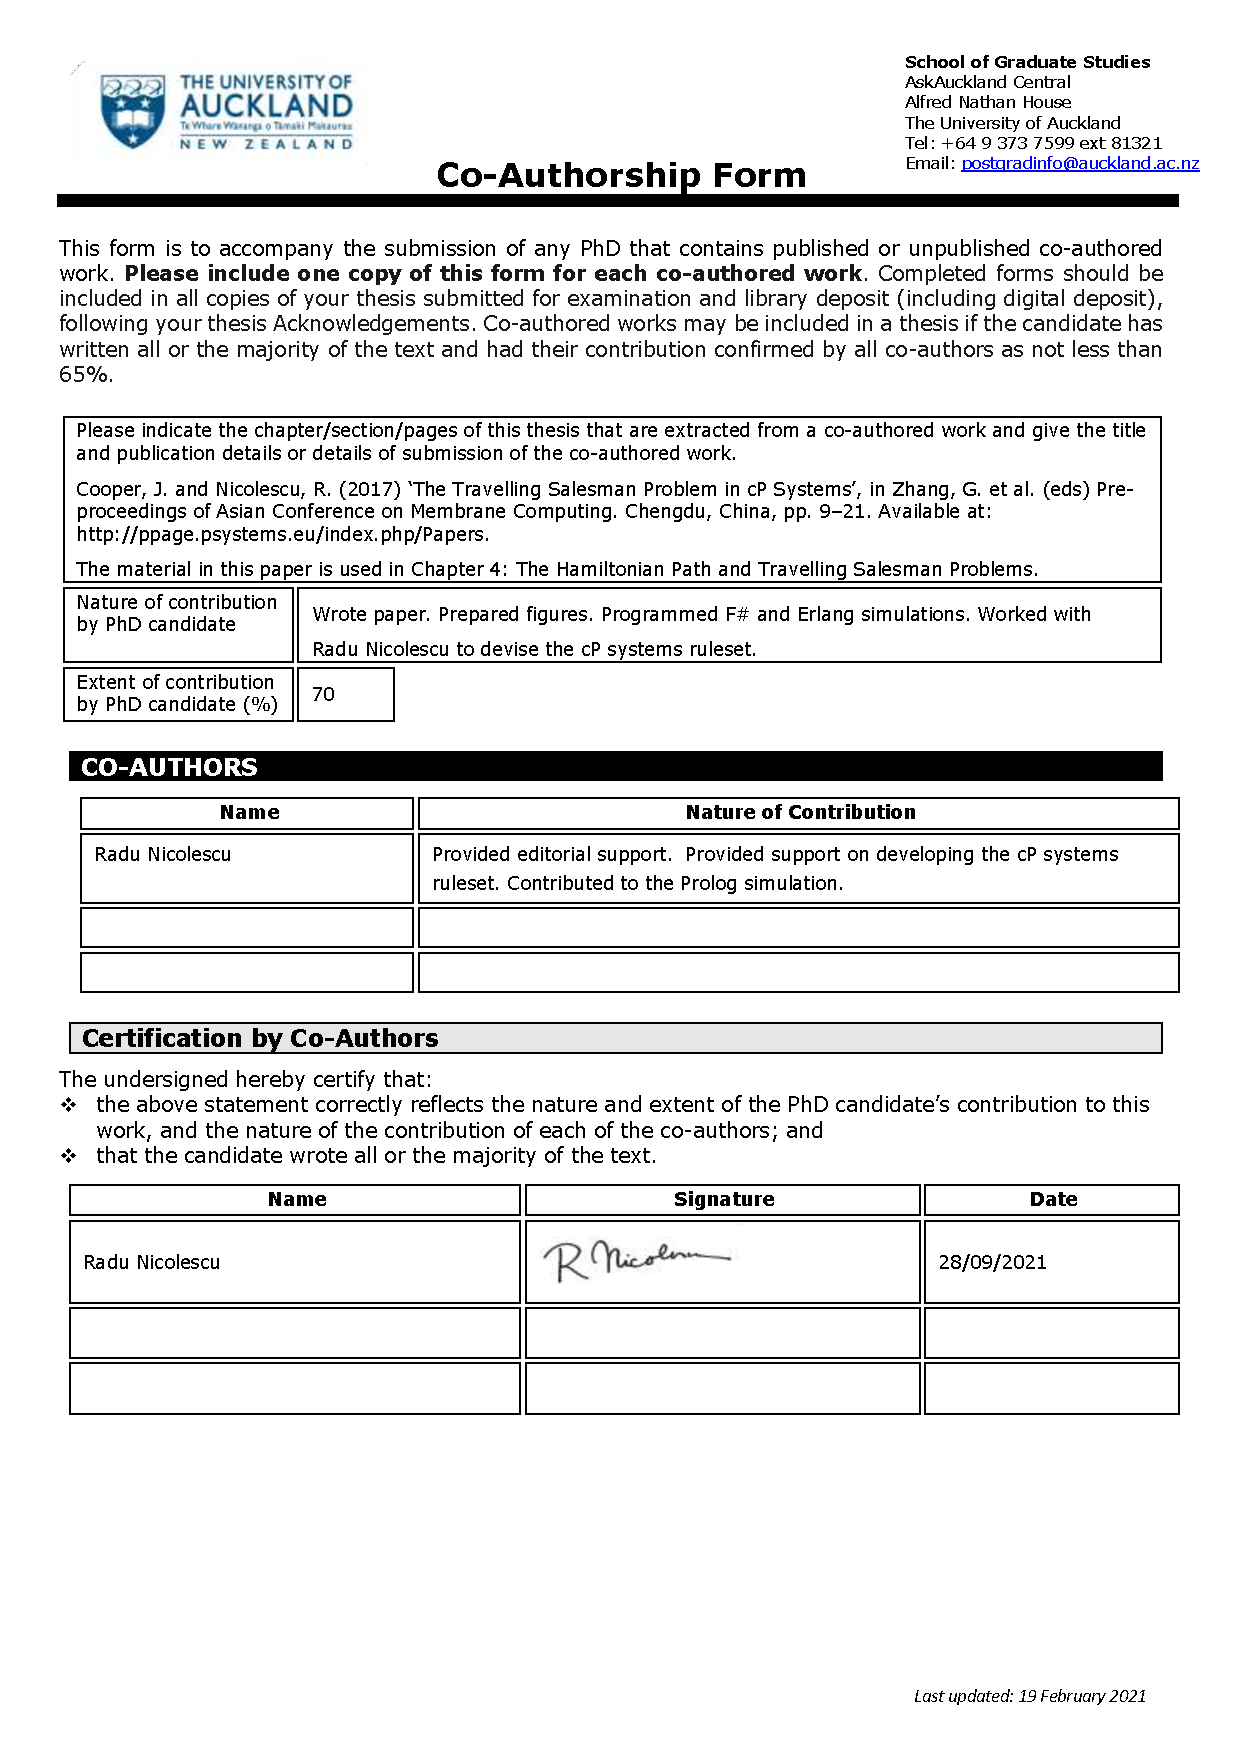
\includepdf{coauthorship_forms/co_authorship_form_conf_tsp.pdf}
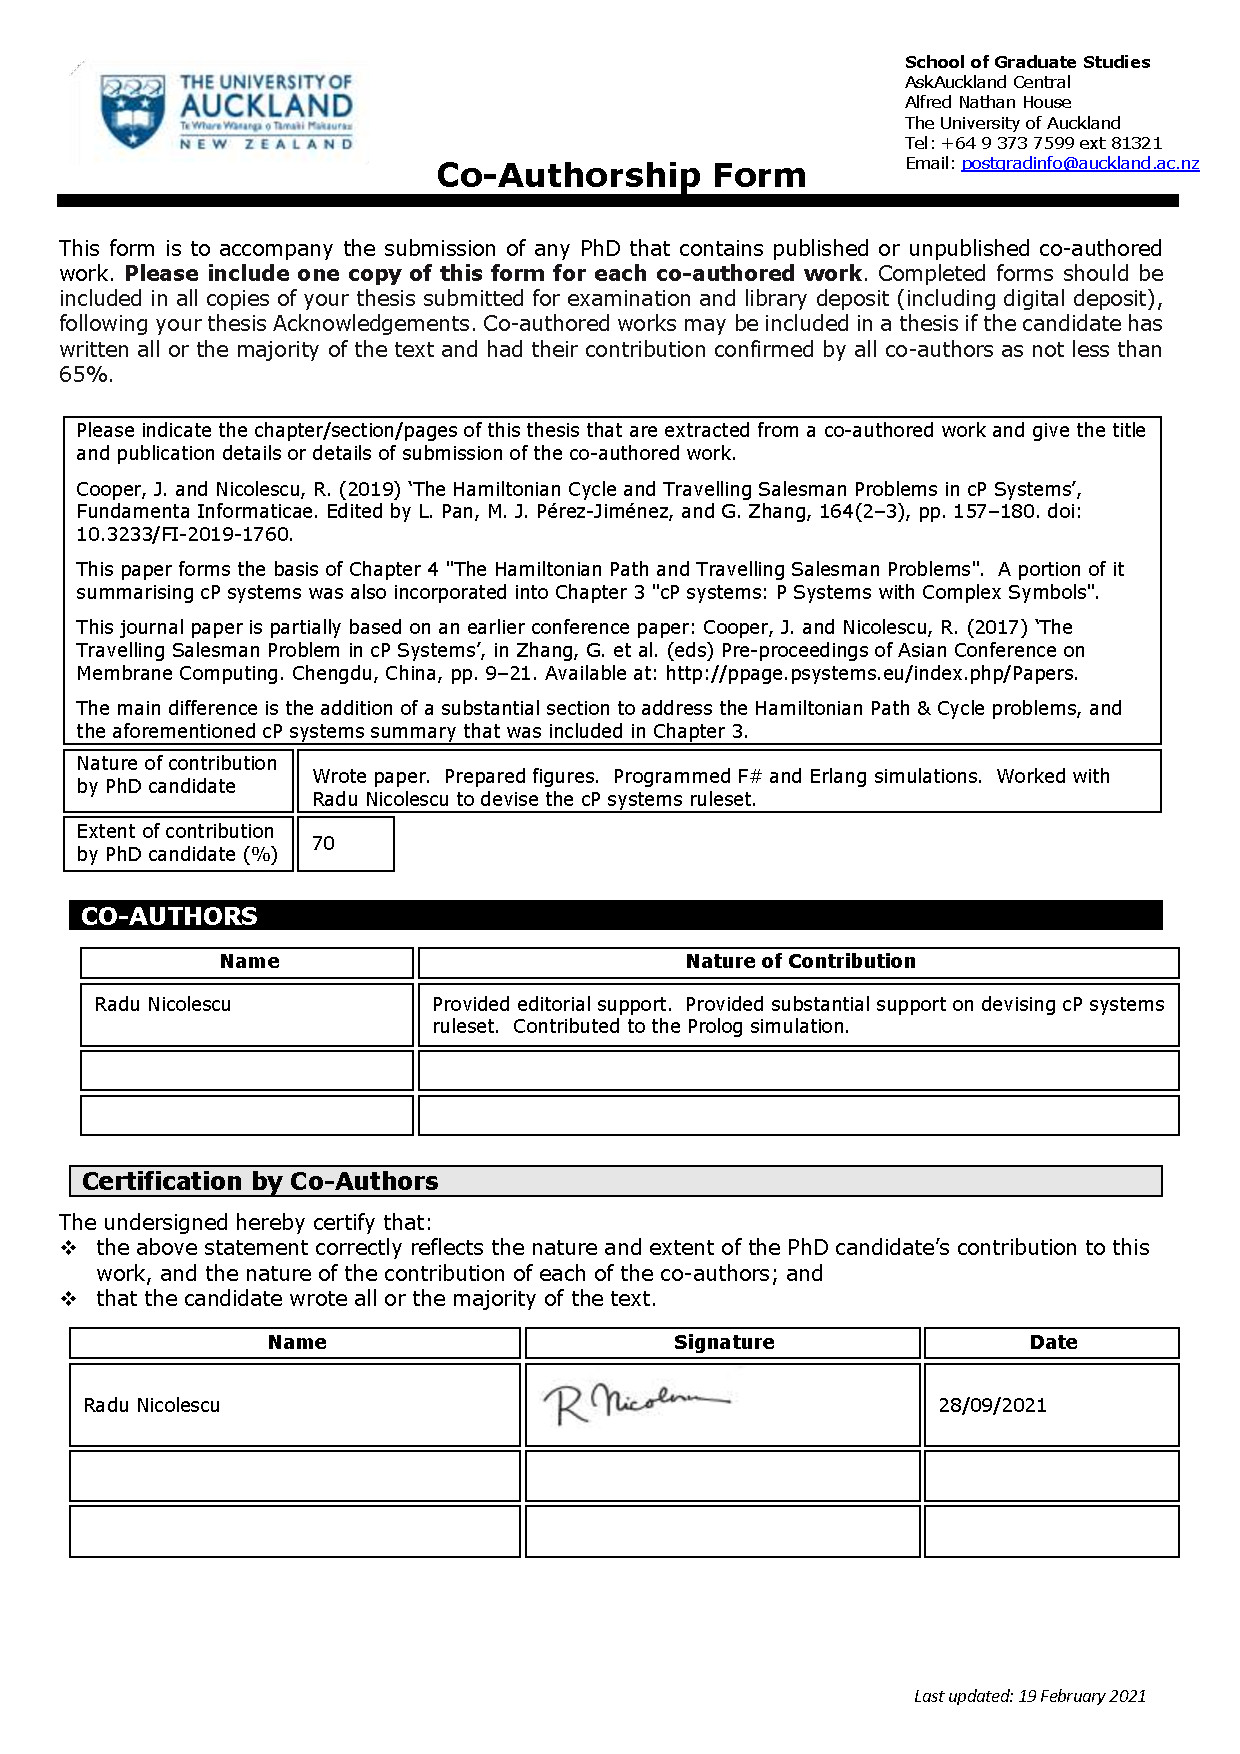
\includepdf{coauthorship_forms/coauthorship_form_HPP_TSP.pdf}
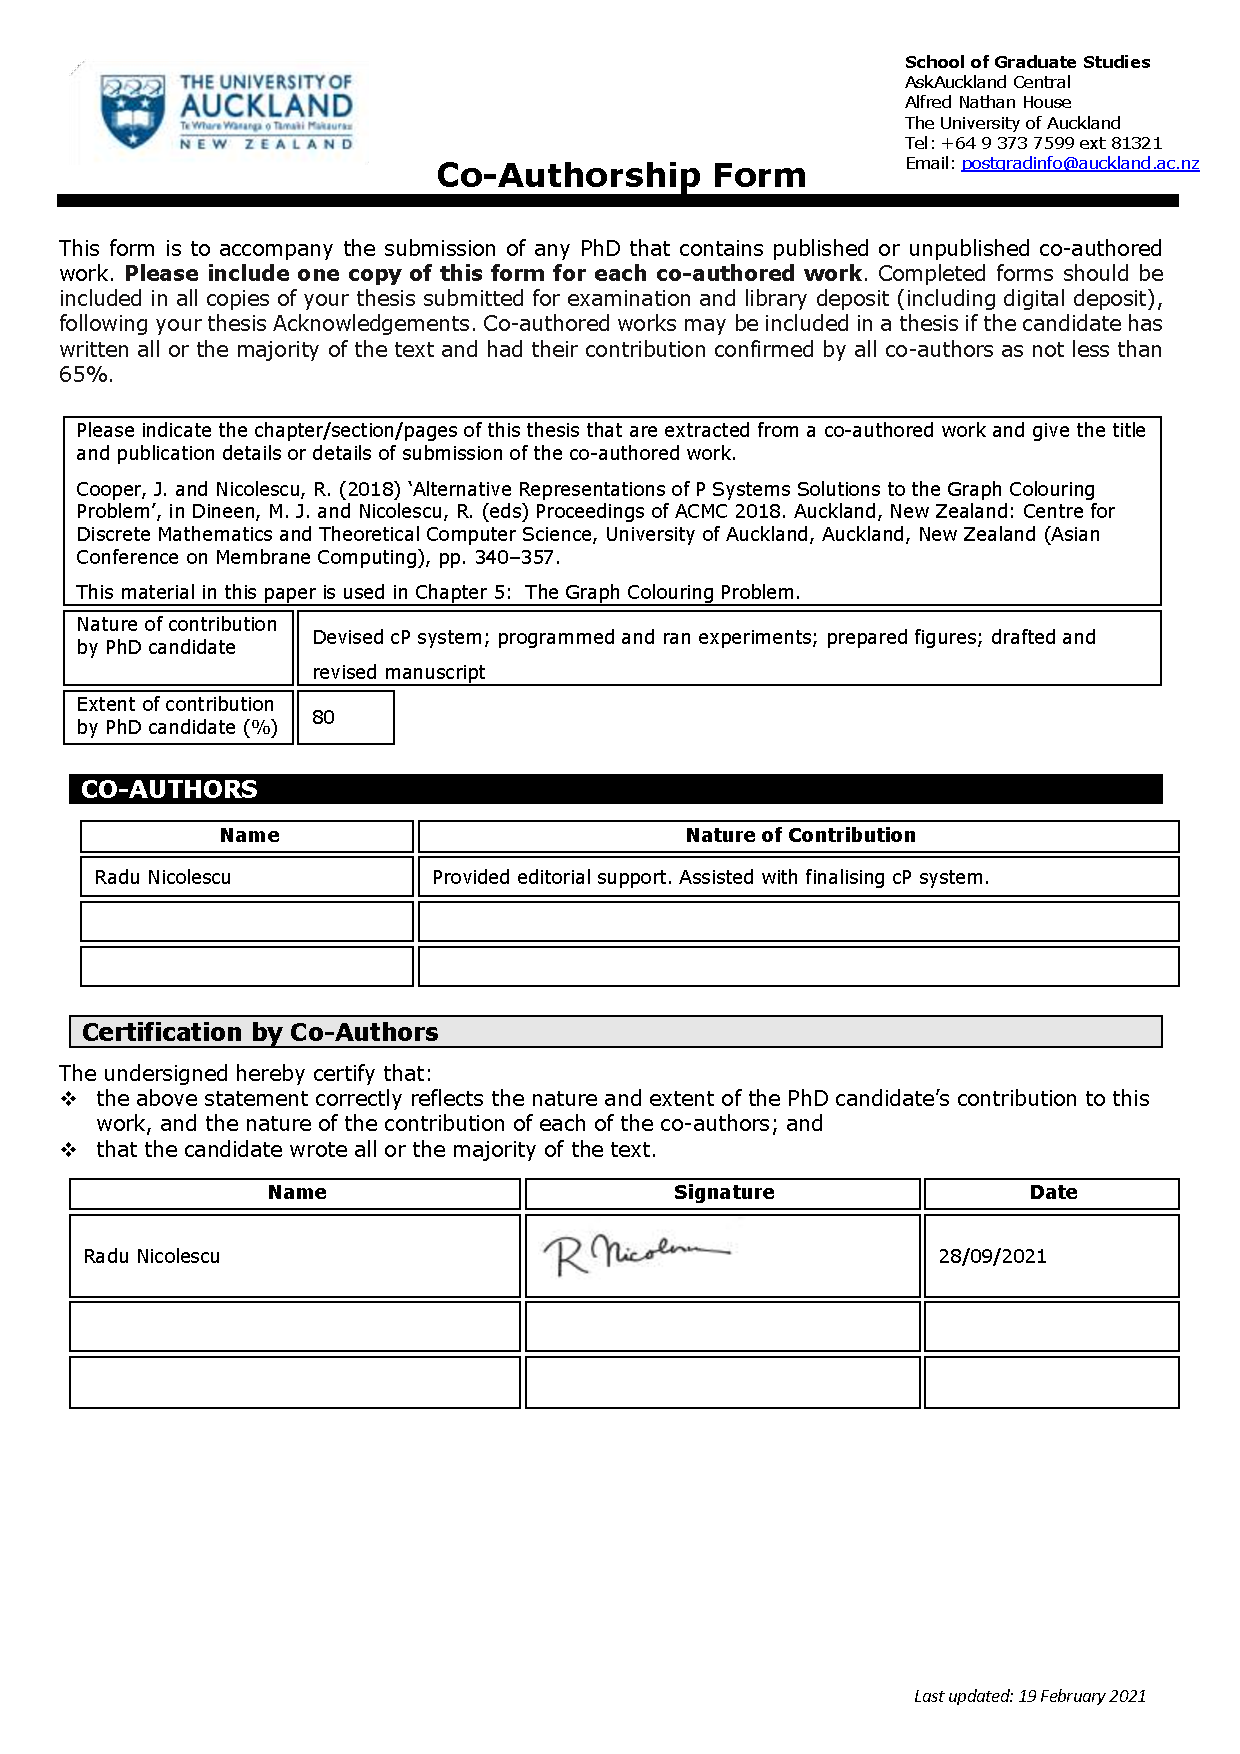
\includepdf{coauthorship_forms/co_authorship_form_conf_gcol.pdf}
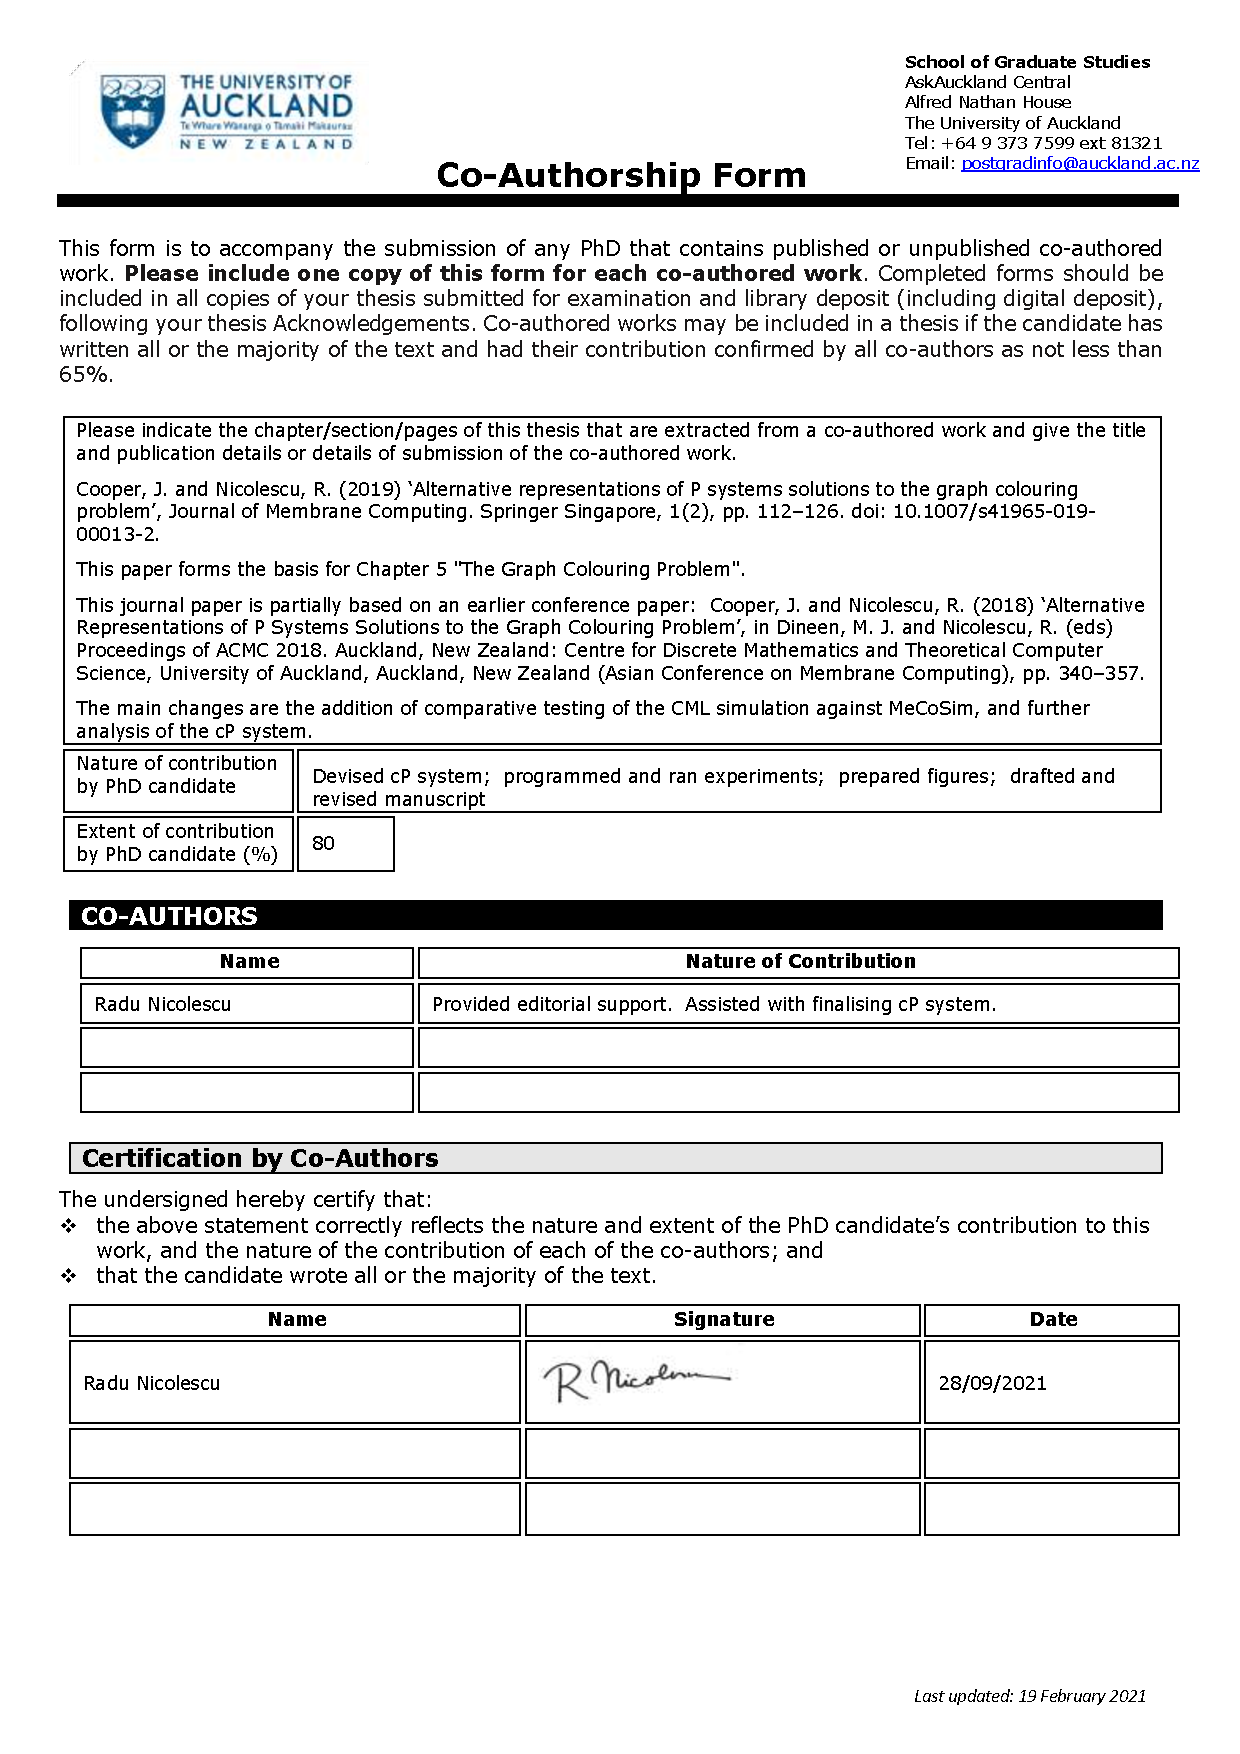
\includepdf{coauthorship_forms/coauthorship_form_GCOL.pdf}
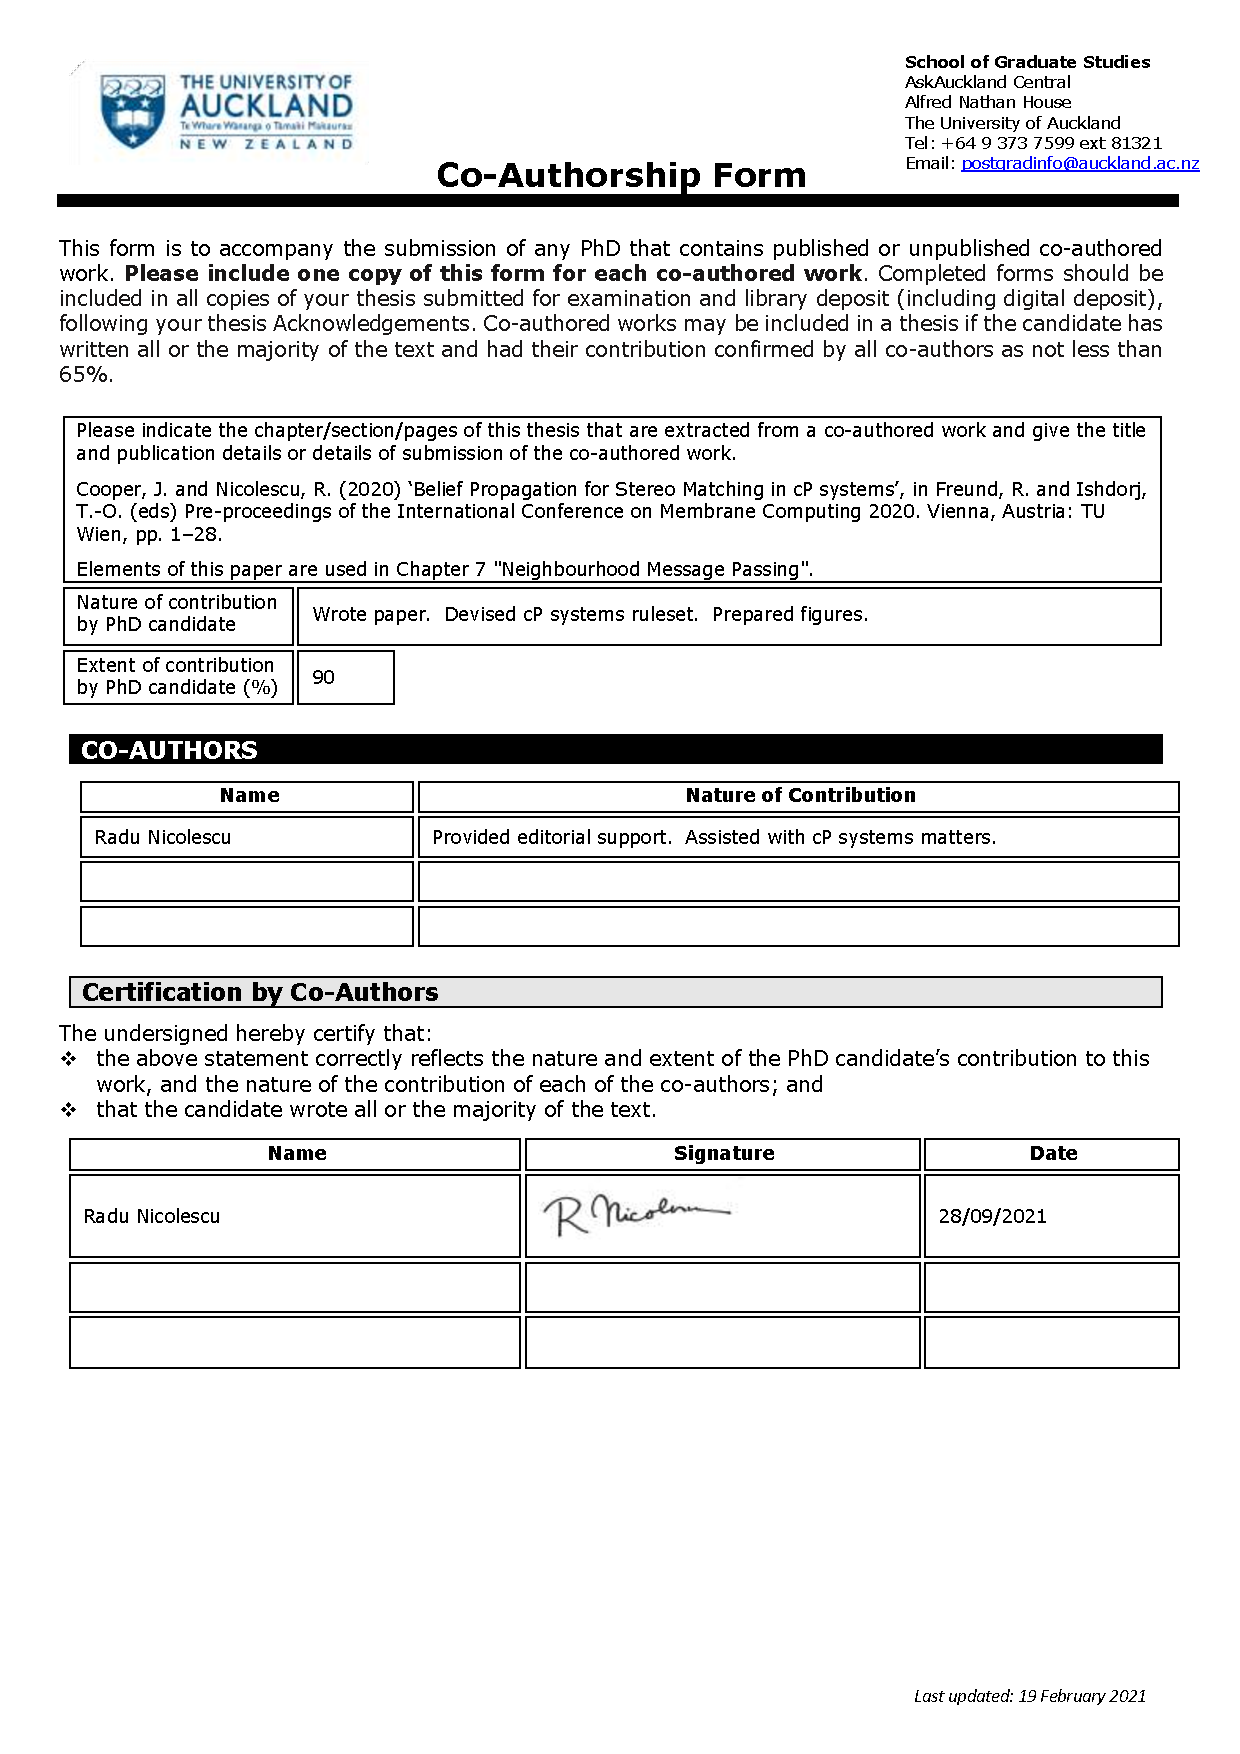
\includepdf{coauthorship_forms/co_authorship_form_conf_bp_cp_systems.pdf}
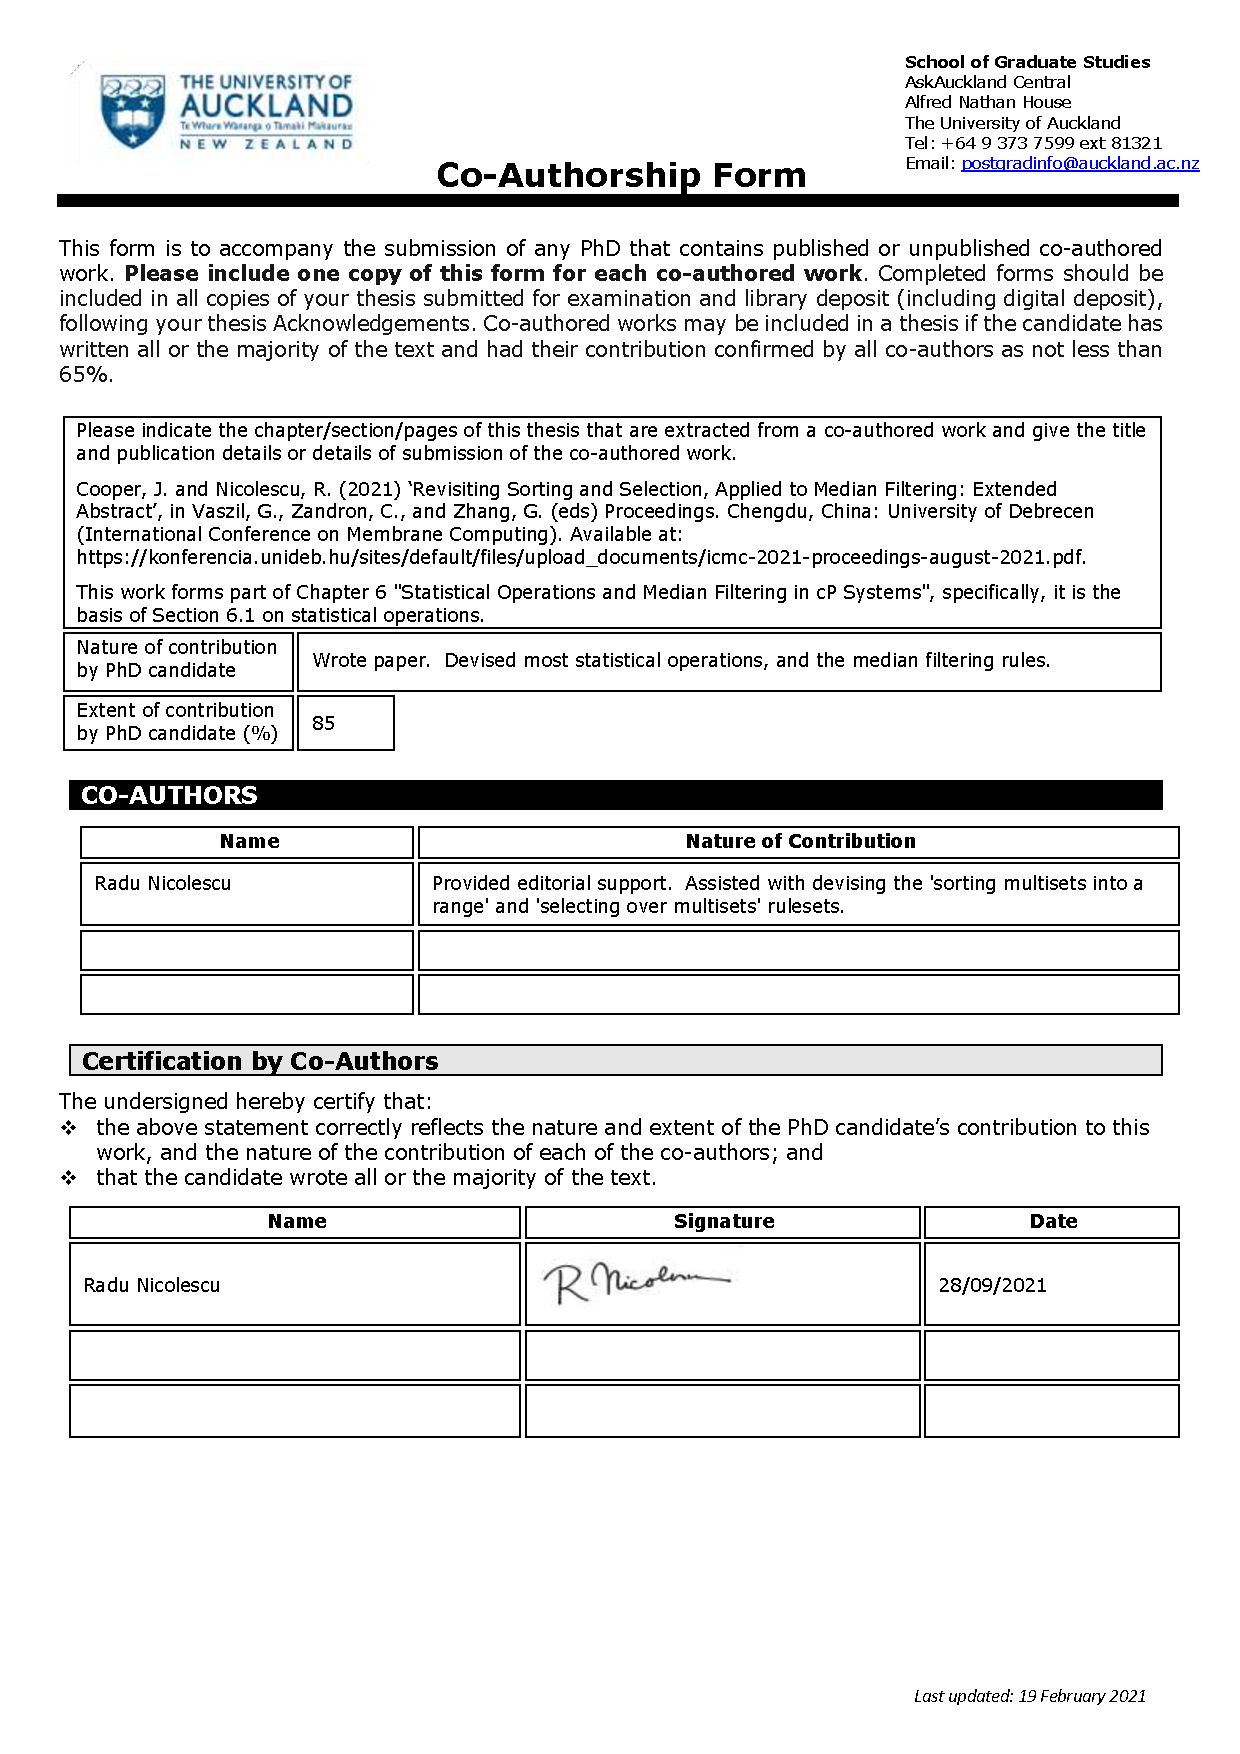
\includepdf{coauthorship_forms/co_authorship_form_cp_systems_stats.pdf}
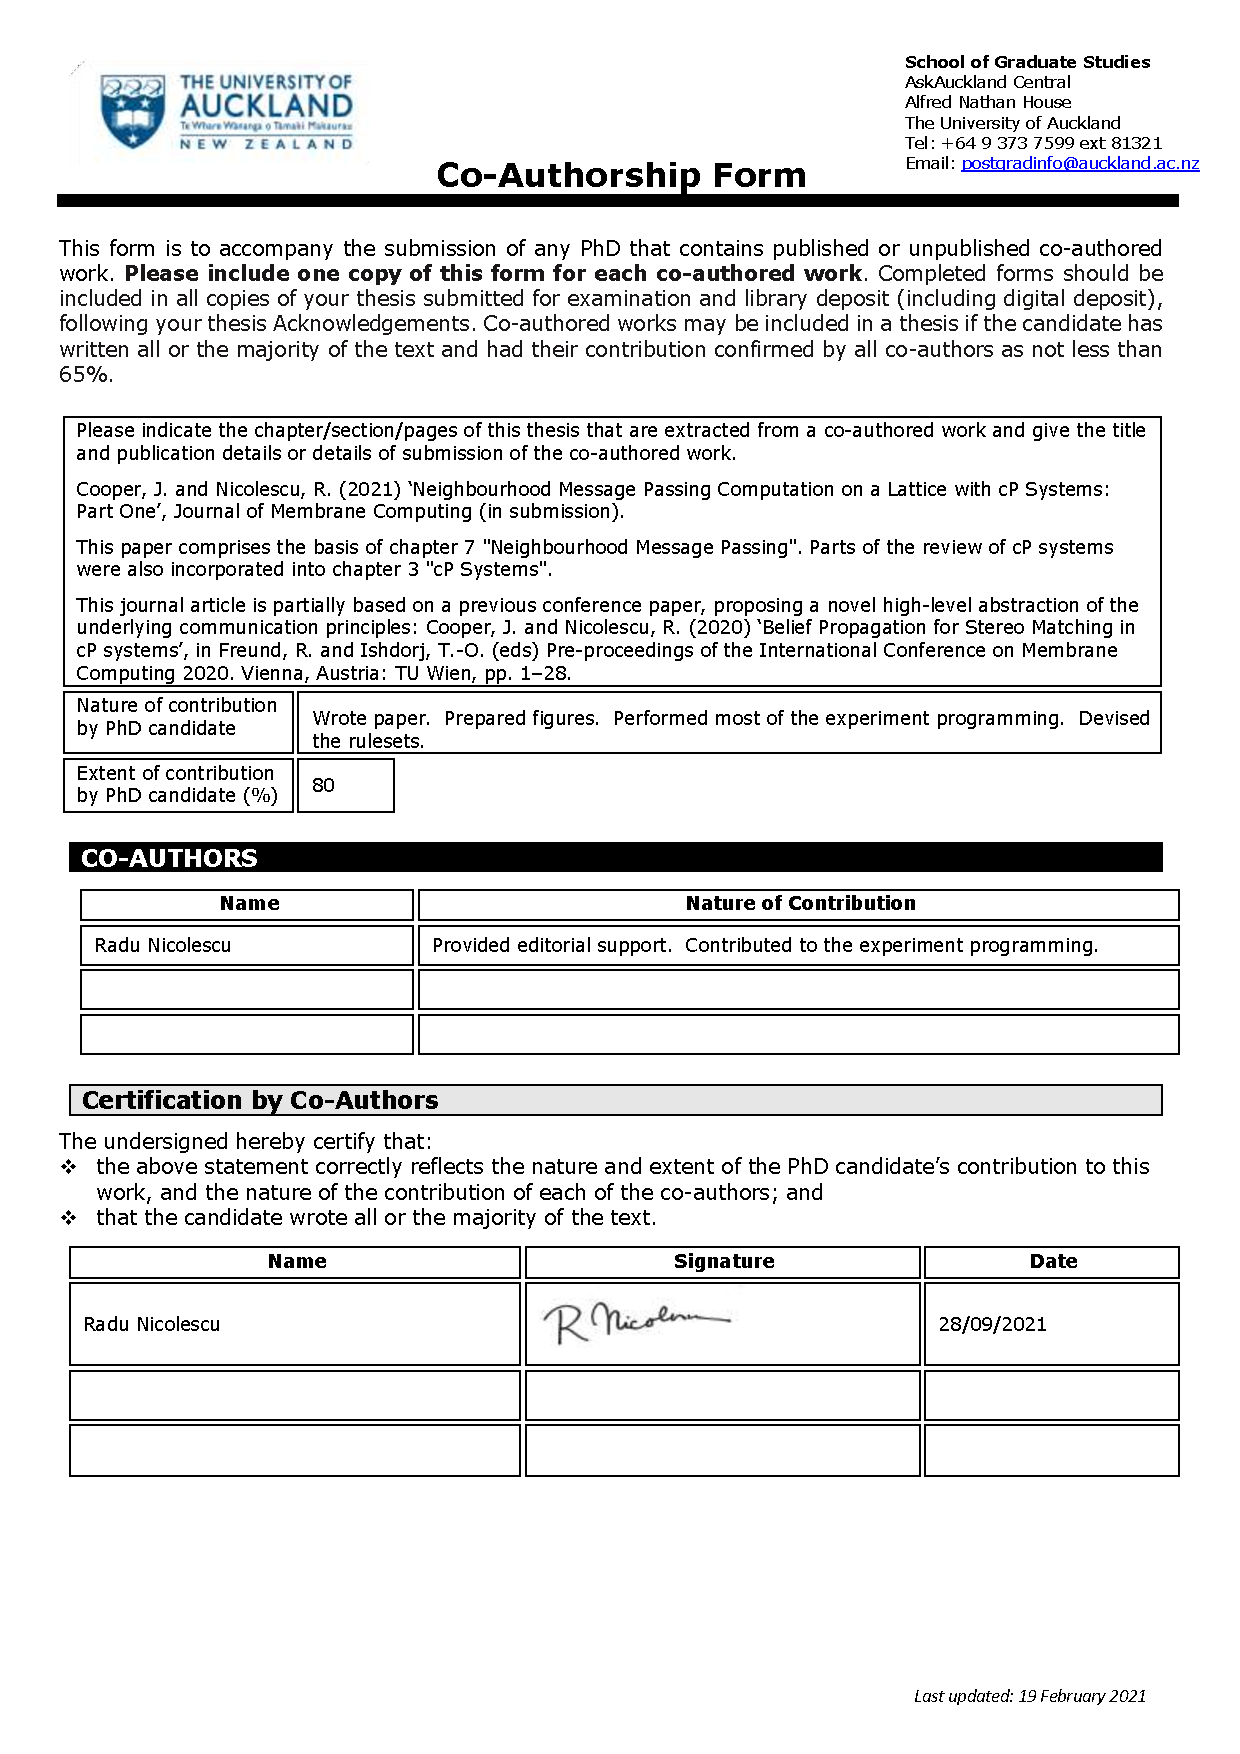
\includepdf{coauthorship_forms/co_authorship_form_nmp.pdf}

% ====================================================
%
% MAINMATTER
%
% Include external chapter files here using
% the \input{} command
%
% If you run out of memory during compilation,
% switch some or all chapters to \include{} instead of \input{}, 
% but watch out for pagination problems.
%
% ====================================================

% \mainmatter

% The below is direct from https://tex.stackexchange.com/a/615994/113430
\mainmatter
\makeatletter
\@mainmattertrue
\makeatother
\setcounter{secnumdepth}{\value{maxsecnumdepth}}

\counterwithin{figure}{chapter}
\counterwithin{table}{chapter}

% \begin{anfxwarning}{Extra glossary entries?}
% Include definitions of promoter and inhibitor in the glossary?
% \begin{itemize}
%     \item antiport
% \end{itemize}
% \end{anfxwarning}

\glsresetall
\chapter{Introduction}

There are many problems in computer science that, from the standpoint of finding a solution quicker, appear amenable to the use of concurrency in their solution.  There are many more where opportunities for concurrency are less apparent and where applying concurrent processing is much less straightforward, but which nevertheless can benefit from it.  For example, many problems that arise in image processing, or which can be modelled graphically, fall into one or the other of those categories.  Modelling these problems with a computational model that embraces concurrency at its core can prove beneficial, both in terms of exposing new ways to structure computations on existing computer implementations, \eg{} \cite{GimelFarb2013a,Nicolescu2014b}, and (potentially) in terms of providing blueprints for the efficient use of new hardware implementations in the future.\footnote{One need only consider the example and future importance of such computing luminaries as Babbage, Lovelace and Boole, all working before a complete working electronic or mechanical computer was created, to see the truth of this.}

This dissertation takes precisely that approach.  Pre-existing problems drawn from the history of computer science are modelled in an inherently concurrent theory of computation, \gls{cps}, seeking the lowest possible theoretical time complexity for each.  Those highly concurrent models are then translated into operative computer programs on current widely available computer hardware.  The theoretical computational model used in this dissertation is \gls{cps} \cite{Nicolescu2018}, one of the branches of the broader field of \gls{mc} (also known as \gls{ps}) \cite{Paun2010b,Paun2002}.  Different hardware, programming languages and techniques have been used in the course of this work, varying based on availability, apparent fit with the relevant \gls{cps} solution, and lessons learned from earlier development.

\Gls{mc} was chosen over other computational models with an emphasis on concurrency because it appears to be a highly promising developing area, especially \gls{cps}.  While \gls{mc} is bio-inspired \cite{Paun2000}, its utility extends far beyond simulating biological systems.  In the original concept (still in use), each \gls{compartment} delimited by a membrane is considered a separate processor with unbounded capacity.  Furthermore, the membranes are frequently considered to have the capability of dividing and creating new membranes and thus processors.  This ability for membrane creation, combined with unbounded space capacity, has long been known to enable polynomial-time solutions to problems that have traditionally been considered intractable by trading space for time \cite{Paun1999a,Sosik2003}.
Other particularly notable calculi are briefly summarised, but the focus of this work is very much on \gls{ps}, and specifically \gls{cps}.

All forms of \gls{ps} operate based on sets of rules associated with delimited \glspl{compartment}, which typically contain multisets of objects. The main advantage of \gls{cps} over other \gls{ps} is its powerful concept of unification (see more in \vref{sec:cps:unification}), which permits the rules to adapt themselves automatically at ``runtime'' to the contents of the relevant \gls{compartment}(s).  By contrast, other forms of \gls{ps} typically require some degree of pre-processing to adapt uniform or semi-uniform families of rules to the given circumstances.  This tends to make interpretation of the rules more difficult, but also can mean that the solution to the problem at hand sometimes is partially pre-computed before the \glspl{ps} ever starts working.

The chief aim of this work is to describe new solutions to pre-existing problems, where the new solutions provide superior time complexity characteristics to other known solutions.  That is, applying relatively new and lesser-known tools of computer science to known problems, with the goal of finding novel solutions with a low time complexity, where low is considered linear complexity -- \bigoh{n} -- or better.  
This is achieved by describing these solutions in \gls{cps}, which is high-level and declarative, and should make each problem's overarching operation and core elements evident.
A secondary aim of this work is to try to find novel, useful ways to implement the proposed solutions to the pre-existing problems on current computers, even when the \gls{cps} model does not map clearly to the hardware.  

% \section{Outline}

% This dissertation proceeds as follows: \Cref{chap:back} summarises some alternative models for concurrent computation -- none of which have quite the same properties as \gls{ps} -- that have been explored in the past; provides an overview of a programming approach called \gls{cml} \cite{Reppy2007,Reppy1991}, which appears to be a good fit in many ways to some of the \gls{cps}; and finally surveys the state of \gls{mc} as at the time of writing.  Next, \cref{chap:cpsystems} fairly comprehensively documents \gls{cps} as used in recent publications.  The various elements of \gls{cps} that have been defined and are still in use -- many of which are used later in this work too -- are shown, before demonstrating how well-known data structures may be modelled in \gls{cps}.  Combined with the examples provided in the subsequent chapters, this should permit the interested reader to start modelling problems in \gls{cps} themselves.

% \Crefrange{chap:tsp}{chap:median} each investigate one or more problems exhibiting significant potential for concurrency.  Specifically: \cref{chap:tsp} focuses on the \gls{hpp}, \gls{hcp} and \gls{tsp} \cite{Applegate2006,Cook2012}; \cref{chap:gcol} on the \gls{gcp} \cite{Lewis2016}; and, \cref{chap:median} on the \gls{medianfilter}, a \gls{mwt} operation performed in image processing \cite{Fisher2016,Gimelfarb2018}.  In each of these chapters, the problem has first been modelled using \gls{cps}, with one or more \glspl{ruleset} developed and analysed, providing a highly concurrent solution to the problem.  Then, the \gls{cps} approach has been investigated empirically, using one or more computer programs, using \gls{cml} in the case of \cref{chap:gcol,chap:median}.  These programs validated the correctness of the \gls{cps} \glspl{ruleset}.  They also sometimes highlight interesting aspects of either the problem or the proposed \gls{cps} solution.

% \Cref{chap:nmp} explores the idea of \gls{nmp}.  Originally motivated by \gls{lbp} \cite{Sun2003,Felzenszwalb2006,Felzenszwalb2011} as used in \gls{sm} \cite{Sinha2020,Tippetts2016,Scharstein2002}, this \lcnamecref{chap:nmp} investigates the situation where individual logical \glspl{pe} are arranged in a lattice and exchange messages as part of computing the solution to a given problem, but every \gls{pe} can only send a message to each connected neighbouring \gls{pe} \emph{after} it has received messages from every other one of its neighbours.  There are two main phases of the core computation process for \gls{nmp}:
% \begin{inparaenum}[a)]
% \item inter-\gls{pe} communications between neighbours via message passing; and
% \item intra-\gls{pe} computations to update internal data and produce new messages.
% \end{inparaenum}  The focus in \cref{chap:nmp} is on the first of these only, with the second abstracted over for current purposes using an oracle with which \glspl{pe} communicate to perform the required updates.

% Finally, \cref{chap:conc} concludes this dissertation by summarising the work described here, and suggesting multiple possible avenues for future research.

% All of \crefrange{chap:tsp}{chap:nmp} provide one or more novel \gls{cps} \glspl{ruleset} with an accompanying explanation, at least one worked example of said \gls{ruleset}, some analysis of the proposed \gls{cps} solution including (where applicable) comparisons to related solutions found elsewhere in \gls{ps}, and the results of at least one experimental computer simulation.

% \section{Key Results}

% The \gls{cps} solutions to the \gls{hpp}, \gls{hcp} and \gls{tsp} in \cref{chap:tsp} all have a time complexity that is linear with respect to the number of nodes in the graph -- \ie{} it is \bigoh{n}, where \(n\) is the order of the graph -- and requires a total of four (for the \gls{hpp}) or five (for the \gls{hcp} and \gls{tsp}) fixed rules for \emph{every} graph with a possible solution.  Simulations are implemented in \fsharp{}, Erlang and Prolog, with the Prolog simulation in particular closely matching the \glspl{cps}.

% \Cref{chap:gcol} experiments with using \gls{cml} to implement a pre-existing \gls{ps} solution to the \gls{gcp}, finding that while the implementation is effective, there is less communication involved than initially expected.  Then, it describes a \gls{cps} solution to the \gls{gcp} which has a time complexity of \bigoh{n}, where \(n\) is the number of nodes in the graph, for graphs where a \(k\)-colouring is possible.  For graphs where no such colouring is possible, it has a time complexity of \bigoh{k}.  \Cref{chap:gcol} represents the first known application of \gls{cml} to any type of \gls{ps} (followed by \cref{chap:median} as the second).

% \Gls{medianfilter}ing is structurally more challenging than many similar \gls{mwt} problems in image processing.  It implies a considerable amount of numerical sorting, and the necessity of preserving the image data prevents the use of typical enhancements to other algorithms, which generally perform a simpler piecewise reduction over the data.  The \glspl{cps} presented in \cref{chap:median} demonstrates conclusively that sufficiently large-scale concurrency can solve the \gls{medianfilter} problem in constant time, however.  The experimental results suggest that current CPUs are far from managing this level of concurrency, though, with the \gls{cml} implementation proving to be by far the slowest --- at minimum 20 times slower than the fastest alternative.

% \Cref{chap:nmp} analyses the traditional \gls{gs} approach to \gls{nmp}, where every \gls{pe} waits until every other \gls{pe} has finished exchanging messages before progressing further itself, and an asynchronous alternative where each \gls{pe} sends the next message to each neighbour as soon as it has received the necessary input messages.  From these, an intermediate \gls{ls} approach where each \gls{pe} waits only for all of its own expected messages to arrive before progressing, arises naturally and is explored also.

% The behaviour and comparative running times required for each variant are investigated empirically, and the \gls{ls} method found strictly superior to the \gls{gs} method -- exhibiting the same messaging behaviour but typically running 5-13\% faster -- while the asynchronous method is, in general, roughly 10\% faster again than the \gls{ls} yet computes final results that ordinarily are within roughly 0.1\% of those of the \gls{ls} method.

\section{Outline and Key Results}

This dissertation proceeds as follows: \Cref{chap:back} summarises some alternative models for concurrent computation -- none of which have quite the same properties as \gls{ps} -- that have been explored in the past;  explains the concept of synchronous vs asynchronous communication in distributed systems (relevant later on);  provides an overview of a programming approach called \gls{cml} \cite{Reppy2007,Reppy1991}, which appears to be a good fit to some of the presented \gls{cps} \glspl{ruleset}; and finally surveys the state of \gls{mc} as at the time of writing.  Next, \cref{chap:cpsystems} fairly comprehensively documents \gls{cps} as used recently.  The various elements of \gls{cps} that have been defined and are still in use -- many of which are used later in this work too -- are shown, before demonstrating how well-known data structures may be modelled in \gls{cps}.  Combined with the examples provided in the subsequent chapters, this should permit the interested reader to start modelling problems in \gls{cps} themselves.

\Crefrange{chap:tsp}{chap:median} each investigate one or more established problems exhibiting significant potential for concurrency.  Specifically: \cref{chap:tsp} focuses on the \gls{hpp}, \gls{hcp} and \gls{tsp} \cite{Applegate2006,Cook2012}; \cref{chap:gcol} on the \gls{gcp} \cite{Lewis2016}; and, \cref{chap:median} on the \gls{medianfilter}, a \gls{mwt} operation performed in image processing \cite{Fisher2016,Gimelfarb2018}.

\Cref{chap:nmp} explores the idea of \gls{nmp}.  Motivated initially by \gls{lbp} \cite{Sun2003,Felzenszwalb2006,Felzenszwalb2011} as used in \gls{sm} \cite{Sinha2020,Tippetts2016,Scharstein2002}, this \lcnamecref{chap:nmp} investigates the situation where individual logical \glspl{pe} are arranged in a lattice and exchange messages as part of computing the solution to a given problem, but every \gls{pe} can only send a message to each connected neighbouring \gls{pe} \emph{after} it has received messages from every other one of its neighbours.  There are two main phases of the core computation process for \gls{nmp}:
\begin{inparaenum}[a)]
\item inter-\gls{pe} communications between neighbours via message passing; and
\item intra-\gls{pe} computations to update internal data and produce new messages.
\end{inparaenum}  The focus in \cref{chap:nmp} is on the first of these only, with the second abstracted over for current purposes using an oracle with which \glspl{pe} communicate to perform the required updates.

All of \crefrange{chap:tsp}{chap:nmp} provide one or more novel \gls{cps} \glspl{ruleset} with an accompanying explanation, at least one worked example of said \gls{ruleset}, analysis of the proposed \gls{cps} solution including (where applicable) comparisons to related solutions found elsewhere in \gls{ps}, and the results of at least one experimental computer simulation.

The \gls{cps} solutions to the \gls{hpp}, \gls{hcp} and \gls{tsp} in \cref{chap:tsp} all have a time complexity that is linear with respect to the number of nodes in the graph -- \ie{} it is \bigoh{n}, where \(n\) is the order of the graph -- and requires a total of four (for the \gls{hpp}) or five (for the \gls{hcp} and \gls{tsp}) fixed rules for \emph{every} graph with a possible solution.  Simulations are implemented in \fsharp{}, Erlang and Prolog, with the Prolog simulation in particular closely matching the \glspl{cps}.

\Cref{chap:gcol} experiments with using \gls{cml} to implement a pre-existing \gls{ps} solution to the \gls{gcp}, finding that while the implementation is effective, there is less communication involved than initially expected.  Then, it describes a \gls{cps} solution to the \gls{gcp} which has a time complexity of \bigoh{n}, where \(n\) is the order of the graph, for graphs where a \(k\)-colouring is possible.  For graphs where no such colouring is possible, it has a time complexity of \bigoh{k}.  \Cref{chap:gcol} represents the first known application of \gls{cml} to any type of \gls{ps} (followed by \cref{chap:median} as the second).

\Gls{medianfilter}ing is structurally more challenging than many similar \gls{mwt} problems in image processing.  It implies a considerable amount of numerical sorting, and the necessity of preserving the image data prevents the use of typical enhancements to other algorithms, which generally perform a simpler reduction over the data.  The \glspl{cps} presented in \cref{chap:median} demonstrates conclusively that sufficiently large-scale concurrency can solve the \gls{medianfilter} problem in constant time, however.  The experimental results suggest that current CPUs are far from managing this level of concurrency, though, with the \gls{cml} implementation proving to be by far the slowest --- at minimum 20 times slower than the fastest alternative.

\Cref{chap:nmp} analyses the traditional \gls{gs} approach to \gls{nmp}, where every \gls{pe} waits until every other \gls{pe} has finished exchanging messages before progressing further itself, and an asynchronous alternative where each \gls{pe} sends the following message to each neighbour as soon as it has received the necessary input messages.  From these, an intermediate \gls{ls} approach where each \gls{pe} waits only for all of its own expected messages to arrive before progressing, arises naturally and is also explored.

The behaviour and comparative running times required for each variant are investigated empirically, and the \gls{ls} method found strictly superior to the \gls{gs} method -- exhibiting the same messaging behaviour but typically running 5-13\% faster -- while the asynchronous method is, in general, roughly 10\% faster again than the \gls{ls} yet computes final results that ordinarily are within roughly 0.1\% of those of the \gls{ls} method.

Finally, \cref{chap:conc} concludes this dissertation by summarising the work described here and suggesting multiple possible avenues for future research.
\glsresetall
\chapter{\label{chap:back}Background}
% This review of past work focuses on the main areas of Computer Science that are relevant to this dissertation.  In none of these cases does the review come close to comprehensively covering the entire span of the given area.  It merely tries to cover as much of the relevant recent and classic work as possible, while giving an extremely brief introduction to these areas.  The interested reader who is unfamiliar with any of these topics is strongly advised to refer to the materials cited.

This \lcnamecref{chap:back} summarises some pertinent related topics that are relevant to the central body of this dissertation.  Each is only a short summary, sufficient to communicate key ideas, provide necessary background information, and demonstrate that there are almost always multiple related theoretical concepts and approaches to solving problems.  In none of these cases does the synopsis come close to comprehensively covering the entire span of the given area.  Each part merely tries to introduce and illuminate its topic sufficiently for the purposes of this work.  The interested reader who is unfamiliar with any of these topics is strongly advised to refer to the materials cited.

% See \url{http://forneylab.org/} for something seemingly quite similar to what I'm doing...;  fglib \url{https://github.com/danbar/fglib};  IGraph library \url{https://igraph.org/};  LGNpy \url{https://github.com/ostwalprasad/LGNpy};

This \lcnamecref{chap:back} specifically discusses formal models of concurrent computation, synchronous \& asynchronous communication, \gls{cml} and \gls{mc}.  \Gls{mc} is, in fact, another model of concurrent computation, but given its central position in this work, it is given a dedicated separate \lcnamecref{sec:back:mc}.  The same can be said about \gls{cps}, which is given its own \lcnamecref{chap:tsp}.

\section{\label{sec:back:formalmodels}Formal Models of Concurrent Computation}
The models briefly reviewed in this \namecref{sec:back:formalmodels} are just a small sample of the formal models for computation that have been devised.  An important aspect of each of the ones mentioned below is that they explicitly deal with concurrency in some fashion, thus meriting their (severely abridged) discussion.  Ultimately, \gls{mc} is used as the model of choice for the remainder of the dissertation after this \namecref{chap:back}, but it undoubtedly has been influenced by, or developed contemporaneously with, each of the below.  Indeed, close study of each model inevitably reveals commonalities between them.

\subsection{\label{subsec:back:csp}Communicating Sequential Processes}

\emph{\Gls{csp}} is a \emph{process algebra} and abstract model of concurrent computation put forward by Hoare \cite{Hoare1985,Roscoe2011}.  A typical sequential computation is represented by a \emph{process}.  Processes' \textcquote[][p.~478]{Roscoe2011}{behaviour is described in terms of the occurrence and availability of abstract entities called \textit{events}}.  Should more than one event be available simultaneously for a given process, then one will be chosen non-deterministically.  This choice is internal to the process, and not influenced by, or visible to, other processes.

Concurrency is introduced by the existence of multiple processes.  In general, the processes continue independently, responding to events as they come.  Should a particular event appear in the alphabet of multiple processes, however, then all processes \emph{must} choose to participate in that event at the same time.  Should all processes involved make such a choice, they engage in a synchronous multi-way atomic synchronisation (hence ``communicating'').  \Gls{csp} has provided significant inspiration for concurrency design in a number of programming languages, notably including Ada \cite{Defense1983,Taft2013}, Occam \cite{Elizabeth1987}, Google's Go \cite{Meyerson2014} (not to be confused with the earlier language Go! \cite{Clark2004}, which itself was explicitly designed for concurrency) and \gls{cml} \cite{Reppy2011} (see further \vref{sec:back:cml}).  An especially interesting practical application of \gls{csp} itself is finding flaws -- and fixes to the flaws -- in information security protocols \cite{Roscoe1995,Lowe1996,Koltuksuz2010}.

\subsubsection{\(\pi\) Calculus}
\(\pi\) calculus was created by Robin Milner and associates in the early 1990s, building upon \gls{csp}.  Milner appreciated \gls{csp}, which advanced concurrency models by explicitly incorporating \emph{synchronised} interaction, something his earlier Calculus for Communicating Systems \cite{Milner1980} had lacked  \cite{Milner1993}.  Milner still regarded \gls{csp} as incomplete, however, in that it had no support for the concept of `mobility' --- \ie{} the ability of the system to reconfigure itself during operation.  In the context of \(\pi\) calculus, this is achieved by passing references to links between processes via other links, thus enabling a dynamic communication system. \(\pi\) calculus was created as an attempt to build upon earlier systems but present a complete calculus of concurrent computation, in much the same way that Lambda Calculus \cite{Barendregt1984} is a complete calculus for sequential computation.\footnote{Milner also noted that sequential computation is a special case of concurrent computation \cite{Milner1993}.}

Both \gls{csp} and \(\pi\) calculus are effective for modelling concurrent systems (see \eg{} \cite{Roscoe2011}).  They have a drawback, however, in that they tend to be very verbose.  Specifications of behaviour for processes are intertwined with the descriptions of processes' states.  They are effective for specifying a system formally, and verifying the behaviour of said system by defined reductions (see \eg{} \cite[Ch.~3.2]{Varela2013}), but for larger systems the notational burden can make it difficult to understand what each process can and will do.

\subsection{\label{subsec:back:actors}\texorpdfstring{\Glspl{actor}}{Actors}}
The \emph{\gls{actor}} model was introduced by Carl Hewitt \cite{Hewitt1973} and substantially further developed for practical programming use by Gul Agha and others \cite{Agha1986,Agha1997}.  Much like \gls{csp} \& its cousins, the \gls{actor} model is based around the concept of sequential, separate but communicating processes which exchange messages.  Again, the processes make decisions independently and proceed based on their communications.  A key difference, however, is that in the \gls{actor} model the message exchanges are \emph{asynchronous}.  Each \gls{actor} has its own \emph{mailbox}, and may send messages to other \glspl{actor} so long as it knows their identity (which is equivalent for this purpose to a concept of a postal address for the \gls{actor}), \emph{but does not wait at all for a response before proceeding}.  Moreover, for \glspl{actor}, the \emph{only} way to communicate with one another is to know the intended recipient's identity/address.  Logical shared memory is explicitly disallowed,\footnote{It is entirely possible in practice, of course, to implement an \gls{actor} system on a shared memory system, but the model expressly forbids any notion of a resource shared in any fashion besides \glspl{actor} requesting a result from another \gls{actor} who has exclusive access to the resource.} which prevents changing who an \gls{actor} communicates with simply by \eg{} changing the holder of a channel endpoint, but also means that actors can be distributed by a runtime without (directly) affecting the practical programming.

The \gls{actor} model is popular for concurrent programming, possibly owing to its intuitive concept.  The fact that communication is asynchronous makes \glspl{actor} much more suitable for modelling distributed systems without shared memory than \gls{csp} or similar --- \glspl{actor} can send messages and proceed without (necessarily) needing to wait for a response, instead continuing forward based on the messages they have received.  By contrast, a typical distributed system with synchronous communication would have prohibitive time costs, given the relative slow speed of typical links between distributed computers as compared to their capacity for local processing.  Many \gls{actor} systems have been implemented for different programming languages (\eg{} \cite{Varela2001,Srinivasan2008,Charousset2016,Bernstein2016}), and in fact it is a core component, and perhaps largely responsible for the success, of Erlang/OTP \cite{Armstrong2010,Armstrong2013,Vinoski2012}.  A relatively new language, Pony \cite{Clebsch2015,Clebsch2017}, takes this even further.

\Glspl{actor}, when used for non-trivial real-world software, have been criticised at times \eg{} \cite{Welsh2013,Stucchio2013}.  While some of the criticisms described are implementation-specific (relating to Akka, a Scala \gls{actor} library), a common thread is that \glspl{actor} do not compose well.  This has the negative consequence that it is difficult to combine an \gls{actor} with anything else to create a new abstraction, and can require extensive modifications in source code to make relatively simple logical changes.

\subsection[GAMMA, the Chemical Abstract Machine, and Join Calculus]{\(\Gamma\), the Chemical Abstract Machine, and Join Calculus}

\subsubsection{\(\Gamma\)}
\citeauthor{Banatre1993} \cite{Banatre1993}, described the \(\Gamma\) (\emph{GAMMA}) ``language'', which uses the multiset as its singular data structure.  The originators stated that their goal with \(\Gamma\) was to create a \enquote{a program structuring tool} focusing on \enquote{logical parallelism} (which seems to be their name for concurrency), rather than creating a working programming language.  Indeed, they acknowledged that translating multiset transformations into programs working on existing electronic computers of the time may prove challenging.  The principal aim was to provide a facility for program designers to state at a high-level the intended transformations, avoiding imposing any ordering on the processing and instead permitting as much concurrency as possible:  \textcquote[][p.~102]{Banatre1993}{our high level of abstraction eliminates unfortunate sequential biases.}  In essence, \(\Gamma\) takes an extreme declarative approach.

Perhaps the largest drawback of \(\Gamma\) is its lack of any form of central control.  All computation is performed through local operations, while \textcquote[][p.~108]{Banatre1993}{the only known solutions to certain problems rely on control decisions involving the whole state of the computation.}  The first problem of such that \citeauthor{Banatre1993} point to is the \gls{gcp} (which is solved in linear time in \cref{chap:gcol} in the present dissertation).  While such problems \emph{can} be solved, expressing the solutions would likely be more, rather than less, complicated than in other systems.  Another criticism that can be levelled at \(\Gamma\) is its lack of formality around its data structure.  Multisets are used, but there is no clear foundation underpinning them.  Rather, in \cite{Banatre1993} both integers and tuples are used as the set elements without any consideration of how they might be constructed or represented.  This is probably appropriate for the extreme high level of \(\Gamma\), but it could impede conversions of its programs to lower level languages more suited to working implementations.

\subsubsection{The Chemical Abstract Machine}
\citeauthor{Berry1992} devised the idea of the \emph{\gls{cham}} \cite{Berry1992}, directly inspired by the concepts from, and building upon, \(\Gamma\).  The parallels between the \gls{cham} and \gls{mc} are clear.  Indeed, the \gls{cham} includes a concept of \glspl{compartment} created by membranes.  Moreover, in his foundational exposition of \gls{mc} \cite{Paun2000}, \citeauthor{Paun2000} directly cites \(\Gamma\) \cite{Banatre1988} and \gls{cham} \cite{Berry1992}.

\(\Gamma\) had a loose notion of being rooted in chemistry, but \gls{cham} significantly adds to the rigour of the analogy, introducing concepts such as molecules composed of atoms, where a system is a collection of such molecules and may be heated or cooled to change the molecular composition.  Where \cite{Banatre1993} made clear the potential of multiset transformations for concurrency, \cite{Berry1992} adds formalisms that enable much more precise specifications of the process of the transformations, without sacrificing the extreme levels of concurrency possible.  The authors demonstrate this fact by showing that \glspl{cham} \enquote{can implement known models of concurrent computation}, including CCS \cite{Milner1980}, mobile processes \cite{Milner1991} and concurrent lambda calculus \cite{Boudol1989}.

\subsubsection{Join Calculus}
Where the \gls{cham} was a development of \(\Gamma\), join calculus is in turn a development of the \gls{cham}.  Join calculus -- created in the 1990s by \citeauthor{Fournet1996} \cite{Fournet1996,Fournet2002} and using the \gls{cham} as its underlying ``machine'' (although, it actually originally targeted \(\pi\) Calculus before switching to the \gls{cham} as a much better fit for its core concepts \cite{Fournet2002}) -- is arguably the most similar in practice of all the models discussed in this \namecref{sec:back:formalmodels} to \gls{mc}.  There are clear common elements between join calculus and \gls{cps}, including heavy use of pattern matching and communication via channels.  Even its reaction rules closely resemble the typical style of rules found in most flavours of \gls{ps} (see \cref{sec:back:mc,chap:cpsystems}).

\citeauthor{Fournet2002} specifically describe join calculus as \textcquote[][p.~269]{Fournet2002}{an attempt to provide language support for asynchronous, distributed, and mobile programming.}  Join calculus has proved fruitful for assisting in the design of new concepts in practical programming, including JoCaml \cite{Fournet2003} (essentially an implementation in OCaml of join calculus as a programming system), Joinads \cite{Petricek2011}\footnote{See also \url{http://tryjoinads.org/docs/use/joins.html}.} and Reagents \cite{Turon2012}.  Despite this utility, however, join calculus seems largely to have been neglected by those outside the theoretical computer science and programming languages communities and appears to have been entirely unused in more recent years.  Later work building on this dissertation could well benefit from an attempt to use join calculus, but it appears less likely to be immediately fruitful than using \gls{mc}.

\subsection[Brane- and Kappa-Calculus]{Brane- and \(\kappa\)-Calculus}
\subsubsection{Brane Calculus}
Brane Calculus\footnote{\citeauthor{Cardelli2005} actually referred to it as Brane \emph{Calculi}, given that he saw it as a family of related systems, but Calculus is used here for consistency with the other described models.} might appear, \foreign{prima facie}, to be the closest relative to \gls{mc} of all the models presented in this \namecref{sec:back:formalmodels}.  The subtitle given to its exposition is \enquote{Interactions of Biological Membranes} \cite{Cardelli2005}.  Both models are undeniably grounded in concepts of cellular biology, with particular emphasis on the cell's membranes.  Both focus heavily on the nesting of those membranes, and movement of items among them.  In actuality, they are dissimilar.

Brane Calculus is as much a system for modelling certain biological processes as it is a computational system.  Importantly, it means that the primitives chosen for it are relatively biologically realistic, and likely much more feasible to implement physically using biology.  While that has some clear potential benefits, it also tends to make even relatively simple systems somewhat difficult to follow.

Brane Calculus also treats its membranes somewhat differently.  In \gls{mc} (certainly \gls{clps}, at least), membranes are used primarily to separate regions of computation and avert undesired interactions between the contents of \glspl{compartment}.  In Brane Calculus, however, much of the processing occurs \emph{on} the membrane itself: \textcquote[][p.~257]{Cardelli2005}{Membranes are not just containers, they are coordinators and active sites of major activity.}  Brane Calculus seems like a promising potential target for an ``intermediate language'' in between \gls{ps} and real biological implementations, but also seems much less useful for expressing the core essence of general computations than \gls{mc}.

\subsubsection{\(\kappa\)-calculus}

Similarly to Brane Calculus, \(\kappa\)-calculus \cite{Danos2004} was introduced as a formal representation of an aspect of cellular biology grounded in prior work in theoretical computer science on concurrent languages.  The focus in \(\kappa\)-calculus is predominantly upon protein interactions, rather than membranes as with Brane calculus: \textcquote[][p.~70]{Danos2004}{Our language idealizes protein-protein interactions, essentially as a particular kind of graph-rewriting}.  This protein focus is demonstrated in \cite{Danos2004} with an example describing part of the digestion process that occurs inside \textit{E.Coli} bacteria, the \enquote{lactose operon}.

The development of \(\kappa\)-calculus may have remained more firmly grounded in traditional concurrency theory than Brane Calculus.  Notably, \citeauthor{Danos2004}, in \textcquote[][p.~76]{Danos2004}{a side observation perhaps only of interest for Concurrency theorists} comment upon their use of \enquote{the ordinary material of process algebras}, pointing out that they use only a minimal subset of the usual operations.  Furthermore, they demonstrated that their simpler (in terms of allowed protein reactions) language \(m\kappa\)-calculus could simulate \(\pi\) calculus, meaning that they could translate systems created in \(\kappa\)-calculus to \(\pi\) calculus and then use programmatic implementations of \(\pi\) calculus, such as Nomadic Pict \cite{Unyapoth2001}, to run those systems on electronic computers.  While this shows that \(\kappa\)-calculus could be used to model solutions to arbitrary problems, it still suffers from the same problem as Brane Calculus.  The modelling for even relatively simple systems quickly becomes quite complex and difficult to read, diminishing the utility of \(\kappa\)-calculus for exploring alternative solutions to known problems in computer science.

\subsection{\label{sec:back:othermodels}Other Models}

\subsubsection{Petri Nets}
Perhaps the earliest formalised model of concurrent computation still in wide use is the \emph{Petri net} \cite{Dennis2011}, first conceived of by Carl Petri to describe chemical processes \cite{Petri2008}.  A basic Petri net consists of places, tokens and transitions, where tokens move between places via arcs and all places are separated by transitions (and \viceversa).

The main weakness of classical Petri nets is that they require the definition of a fixed system from the outset, and do not easily permit the evolution of the system during ``runtime'' as appropriate.  Of Petri nets, \citeauthor{Varela2013} says \textcquote[][p.~36]{Varela2013}{Petri nets \textelp{} in the \textelp{} form described \textins{in \cite{Varela2013}}, \textelp{} are not able to model the dynamicity of concurrent software\textins{.}  \textelp{} Petri nets \textelp{} do not support the compositional reasoning afforded by more modern models of concurrency.}

\subsubsection{\label{sec:back:pram}Parallel Random Access Machines}

\emph{\Glspl{pram}} are a model for concurrent computation arguably closer to the operation of real electronic computers than the others described above.  \citeauthor{JaJa2011} defines a \gls{pram} as \textcquote{JaJa2011}{an abstract model for parallel computation which assumes that all the processors operate synchronously under a single clock and are able to randomly access a large shared memory. In particular, a processor can execute an arithmetic, logic, or memory access operation within a single clock cycle}.  Unlike the process algebras described above, the \gls{pram} model does not, in general, impose a particular way to describe a \gls{pram} algorithm, making it sometimes quite seful in developing parallel algorithms.

\Glspl{pram} developed as a natural extension to random access machines (RAMs), which, as the name suggests, provide a model that is reasonably close to typical uniprocessor electronic computers.  A \gls{pram} is a collection of processors operating synchronously (\ie{} on the same clock), each labelled with a unique identifier, and with access to a global shared memory.  Processors may operate independently of each other, but many described \gls{pram} algorithms in fact operate in a \emph{single-program multiple-data} fashion where all processors follow the same program and so are only semi-independent, at best.  These attributes mean that a \gls{pram} often looks quite similar (at a superficial level, at least) to the operation of a typical \gls{gpu}.  The systems described in \cref{chap:nmp} also bear more than a passing resemblance to \glspl{pram}.
%-------------------------------------------------------
\section{\label{sec:back:syncasync}Synchronous and Asynchronous Messaging in Distributed Algorithms}
%-------------------------------------------------------

This dissertation uses the standard timing models in distributed algorithms \cite{Lynch1996} for messaging where relevant.  For reference, the most important relevant concepts are explained and illustrated below.  For more on the topics discussed in this \namecref{sec:back:syncasync}, the interested reader is referred to \cite{Fokkink2013,Lynch1996,Tel2000}.

\subsection{Rounds}
Under both synchronous and asynchronous messaging, all processes work in \emph{rounds} (sometimes also referred to as \emph{macro-steps}).  A round consists of three repeating sequential sub-steps:
\begin{enumerate}
    \item \emph{\textsf{Receive}}:  receive one or more incoming messages
    \item \emph{\textsf{Process}}:  perform any requisite local computations as induced by the received messages, and update the local state
    \item \emph{\textsf{Send}}:  send out new messages as appropriate based on the processing from the previous step
\end{enumerate}
This applies only to messaging between processes.  For systems with a solitary process, there is no meaningful concept of rounds because the process will essentially remain in the \textsf{process} sub-step.  \Ie{} a lone process will continue working without messaging until the system halts (if ever).

\subsection{Synchronous Messaging}
Under the synchronous model, all processes proceed in lock-step.  They may carry out the sub-steps at different speeds, but begin and end rounds together.  When considering timing of messaging, there are two standard approaches:  to consider the \textsf{process} sub-step as taking one time unit and the transit time -- the time between when the message is sent by the sender and when it is received by the recipient -- taking zero time units; or, to consider the \textsf{process} sub-step as taking zero time units and the transit time taking one time unit.

\subsection{Asynchronous Messaging}
Under the asynchronous model, there is (unsurprisingly) no natural synchronisation between processes.  All processes proceed through the sub-steps at their own pace.  The \textsf{process} sub-step is considered to take zero time units, and message transit times are considered to take any number of time units.  Alternatively, by normalisation, while the \textsf{process} sub-step still takes zero time units, message transit times take somewhere between zero and one (inclusive) time units.  This makes the second synchronous approach a special case of the asynchronous approach.  The asynchronous model is similar to the theoretical \gls{actor} model.

\subsection{Echo}
To illustrate the difference between the synchronous and asynchronous scenarios, consider the illustrations in \cref{fig:back:echosync,fig:back:echoasync}.\footnote{These figures were created by Dr. Radu Nicolescu, and have been reproduced here with his permission.}  The \textsf{echo} algorithm \cite[Ch.~4.3]{Fokkink2013} is used to establish a spanning tree over a graph of nodes/processes, in this case rooted at node 1.  The algorithm works in two phases, named \emph{broadcast} and \emph{convergecast}.  \textsf{Echo} starts in the broadcast phase with an initiator node sending out a broadcast message to each of its neighbours.  Each of those recipients then marks the sender as its parent, sends a broadcast message to every other one of its neighbours, then waits to receive a broadcast message from each of those other neighbours.  This pattern repeats across the graph.  Once the response broadcast messages are received, each node then sends a convergecast message back to its parent.  This carries on until finally the initiator receives the convergecast messages back from its neighbours.

In \cref{fig:back:echosync,fig:back:echoasync}, the first green node is the initiator, and each other node turns green when it receives its first message.  Edges between nodes turn into green arrows when a node chooses its parent.  The direction of the arrow points to said parent.  Red arrows indicate the direction of travel for a broadcast message, while blue arrows indicate the direction of travel for a convergecast message.  Solid red \& blue arrows indicate that a message is received in that round by the recipient, while a dashed line indicates that the message is still in transit.

\begin{figure}[htbp]
    \centering
    \subcaptionbox{Round Zero}{\includegraphics[width=0.32\textwidth]{chapters/background/images/echo/sync/notext_f0_0.pdf}}
    \subcaptionbox{Round One}{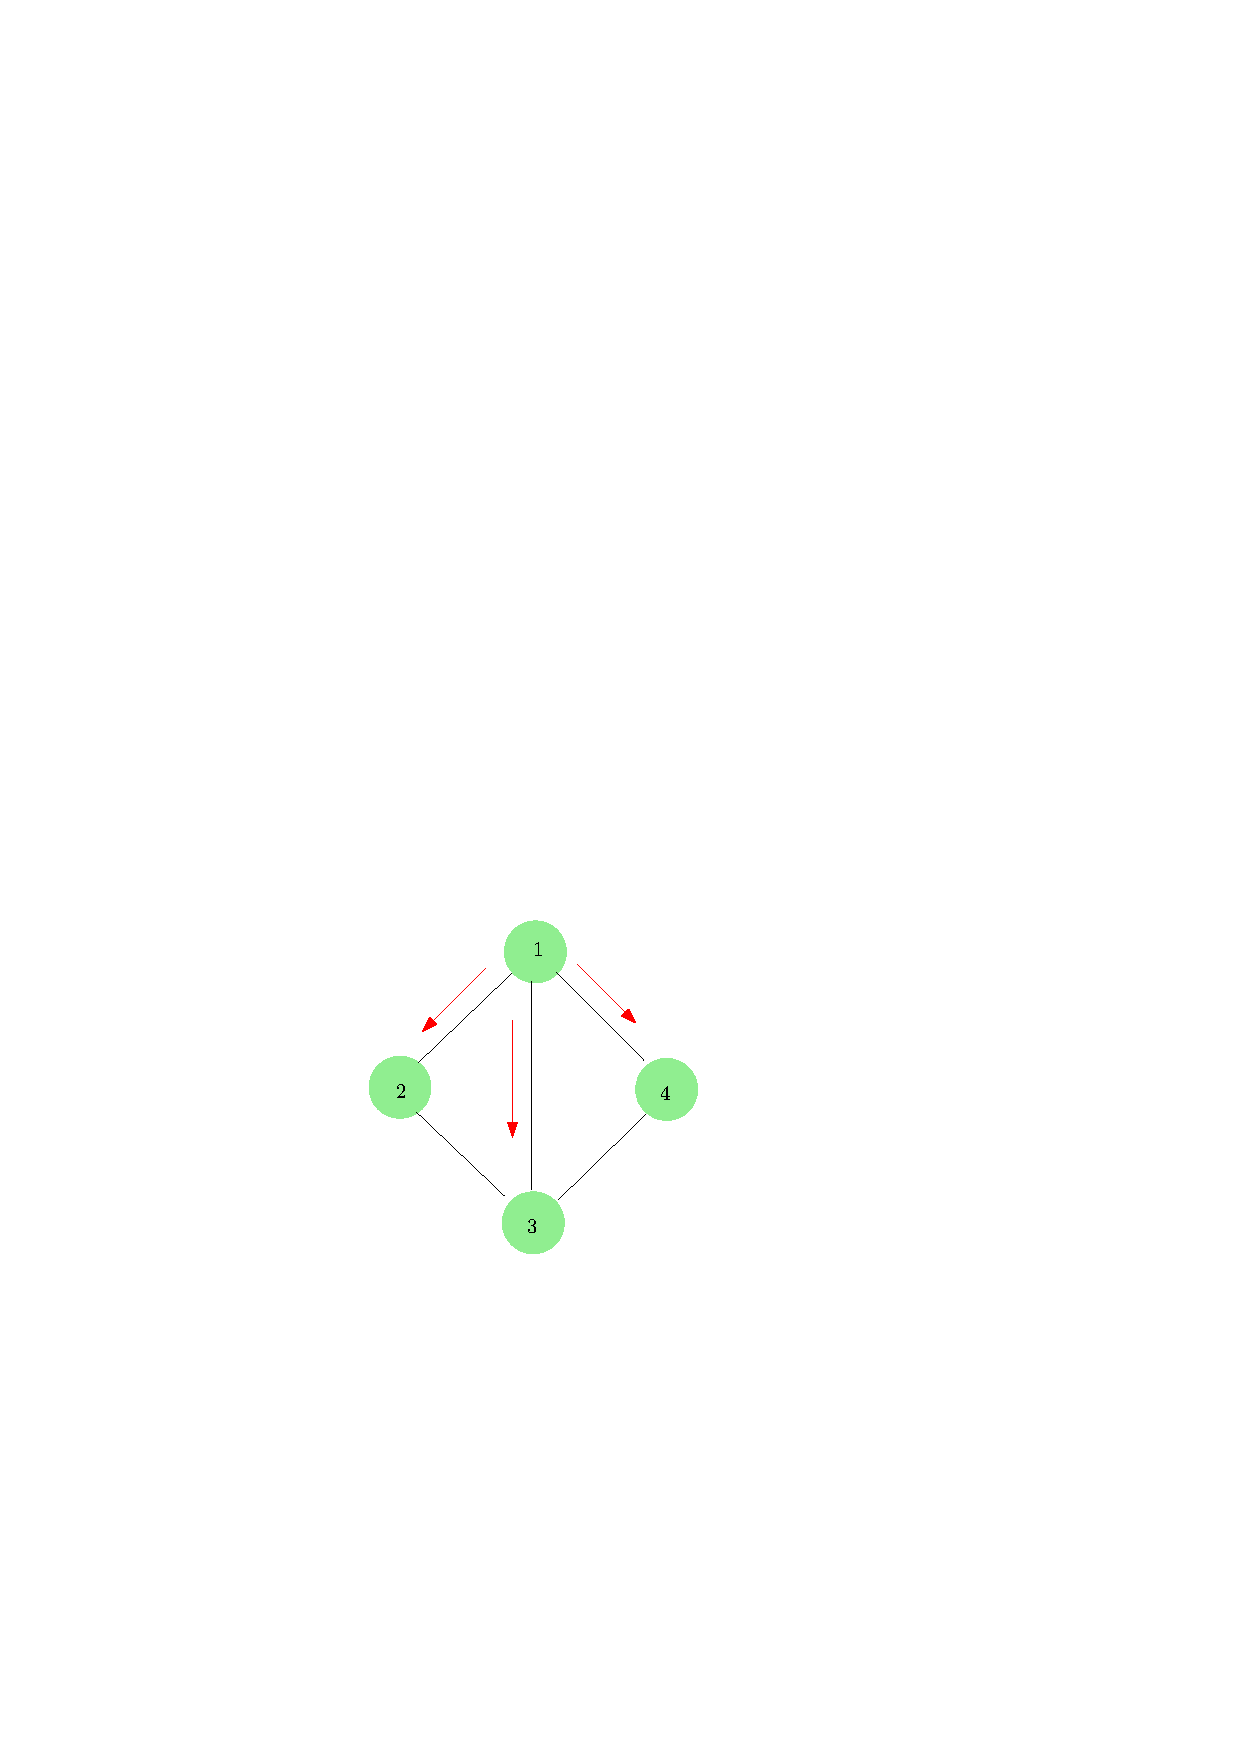
\includegraphics[width=0.32\textwidth]{chapters/background/images/echo/sync/notext_f0_1.pdf}}
    \subcaptionbox{Round Two}{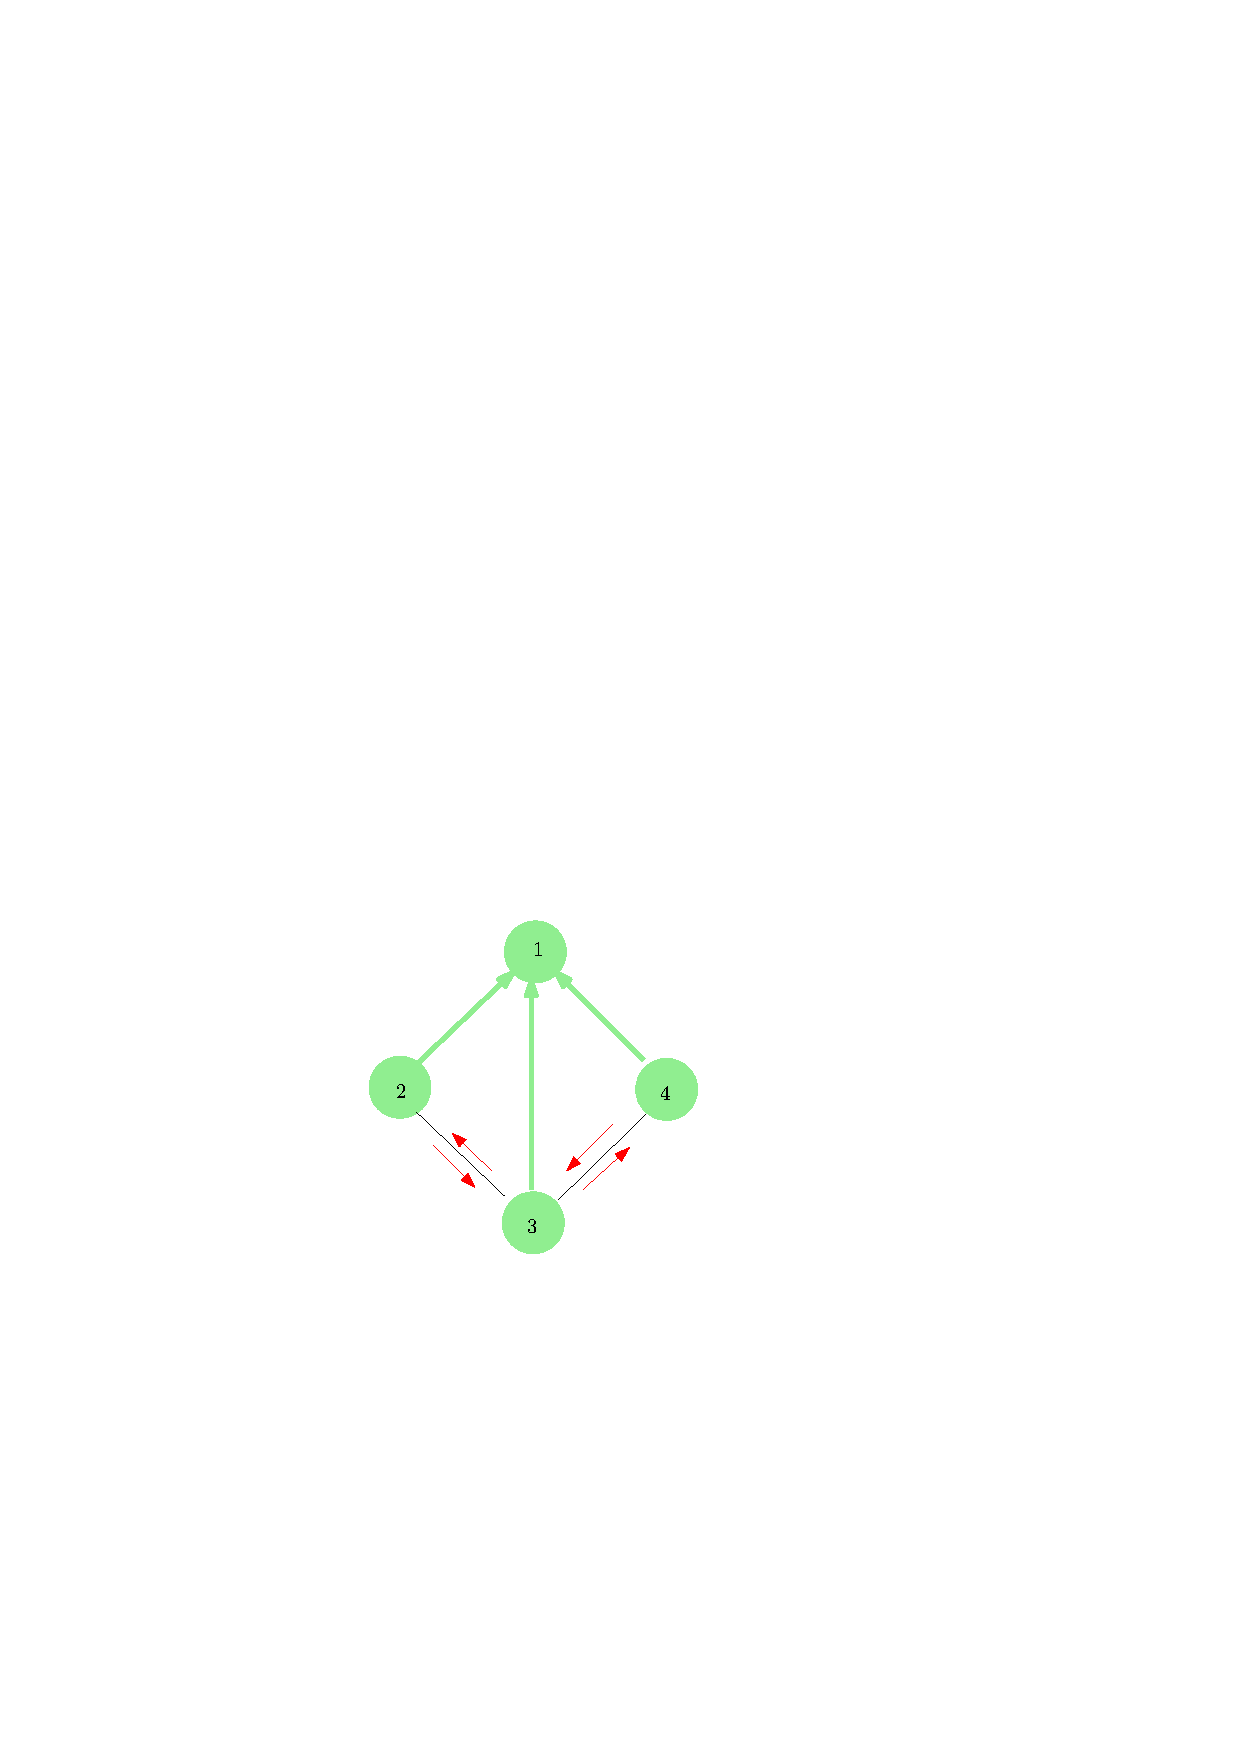
\includegraphics[width=0.32\textwidth]{chapters/background/images/echo/sync/notext_f0_2.pdf}}
    \subcaptionbox{Round Three}{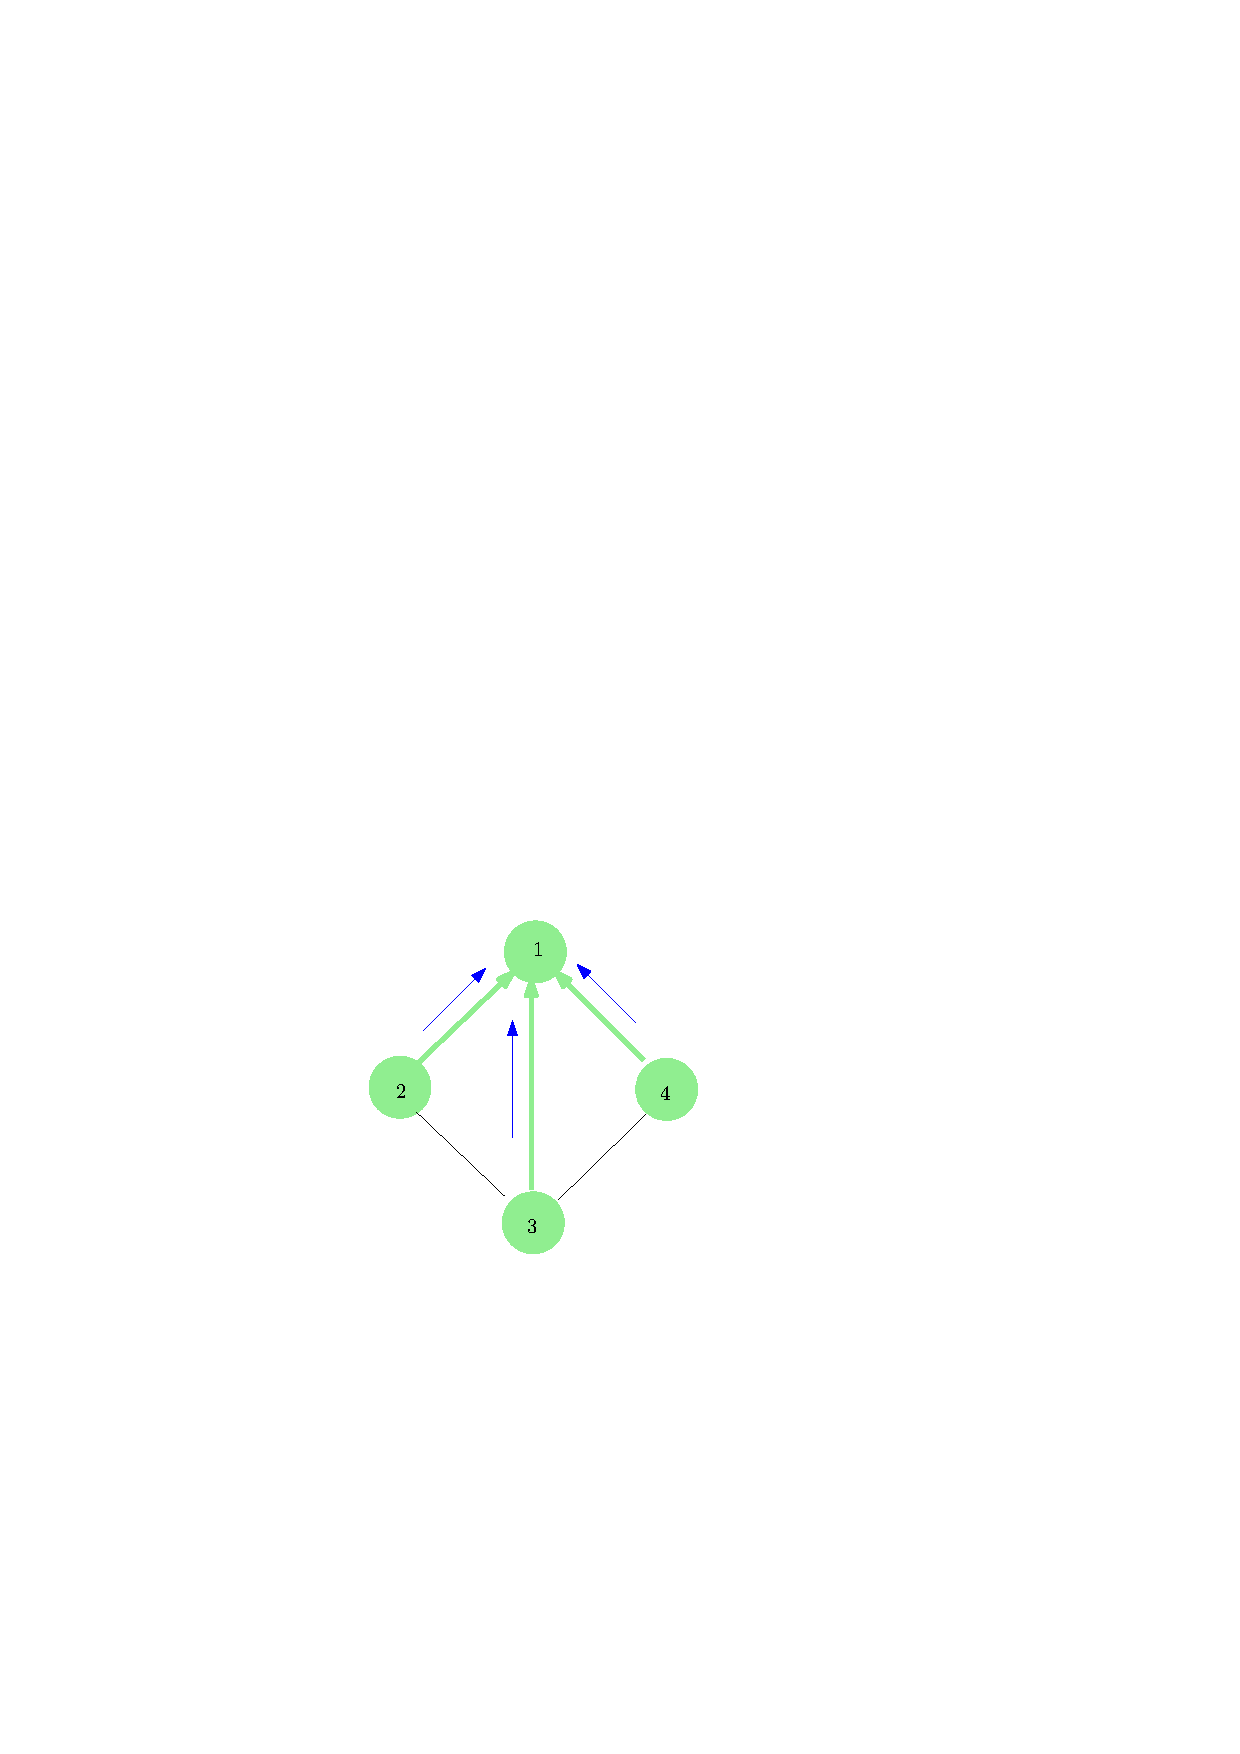
\includegraphics[width=0.32\textwidth]{chapters/background/images/echo/sync/notext_f0_3.pdf}}
    \caption[Progression of the synchronous \textsf{echo} algorithm]{Progression of the synchronous \textsf{echo} algorithm, starting from round zero before any messages are sent.  Arrows in red mean broadcast messages, while arrows in blue mean convergecast messages.}
    \label{fig:back:echosync}
\end{figure}

\begin{figure}[htbp]
    \centering
    \subcaptionbox{Round Zero}{\includegraphics[width=0.32\textwidth]{chapters/background/images/echo/async/notext_f0_0.pdf}}
    \subcaptionbox{Round One}{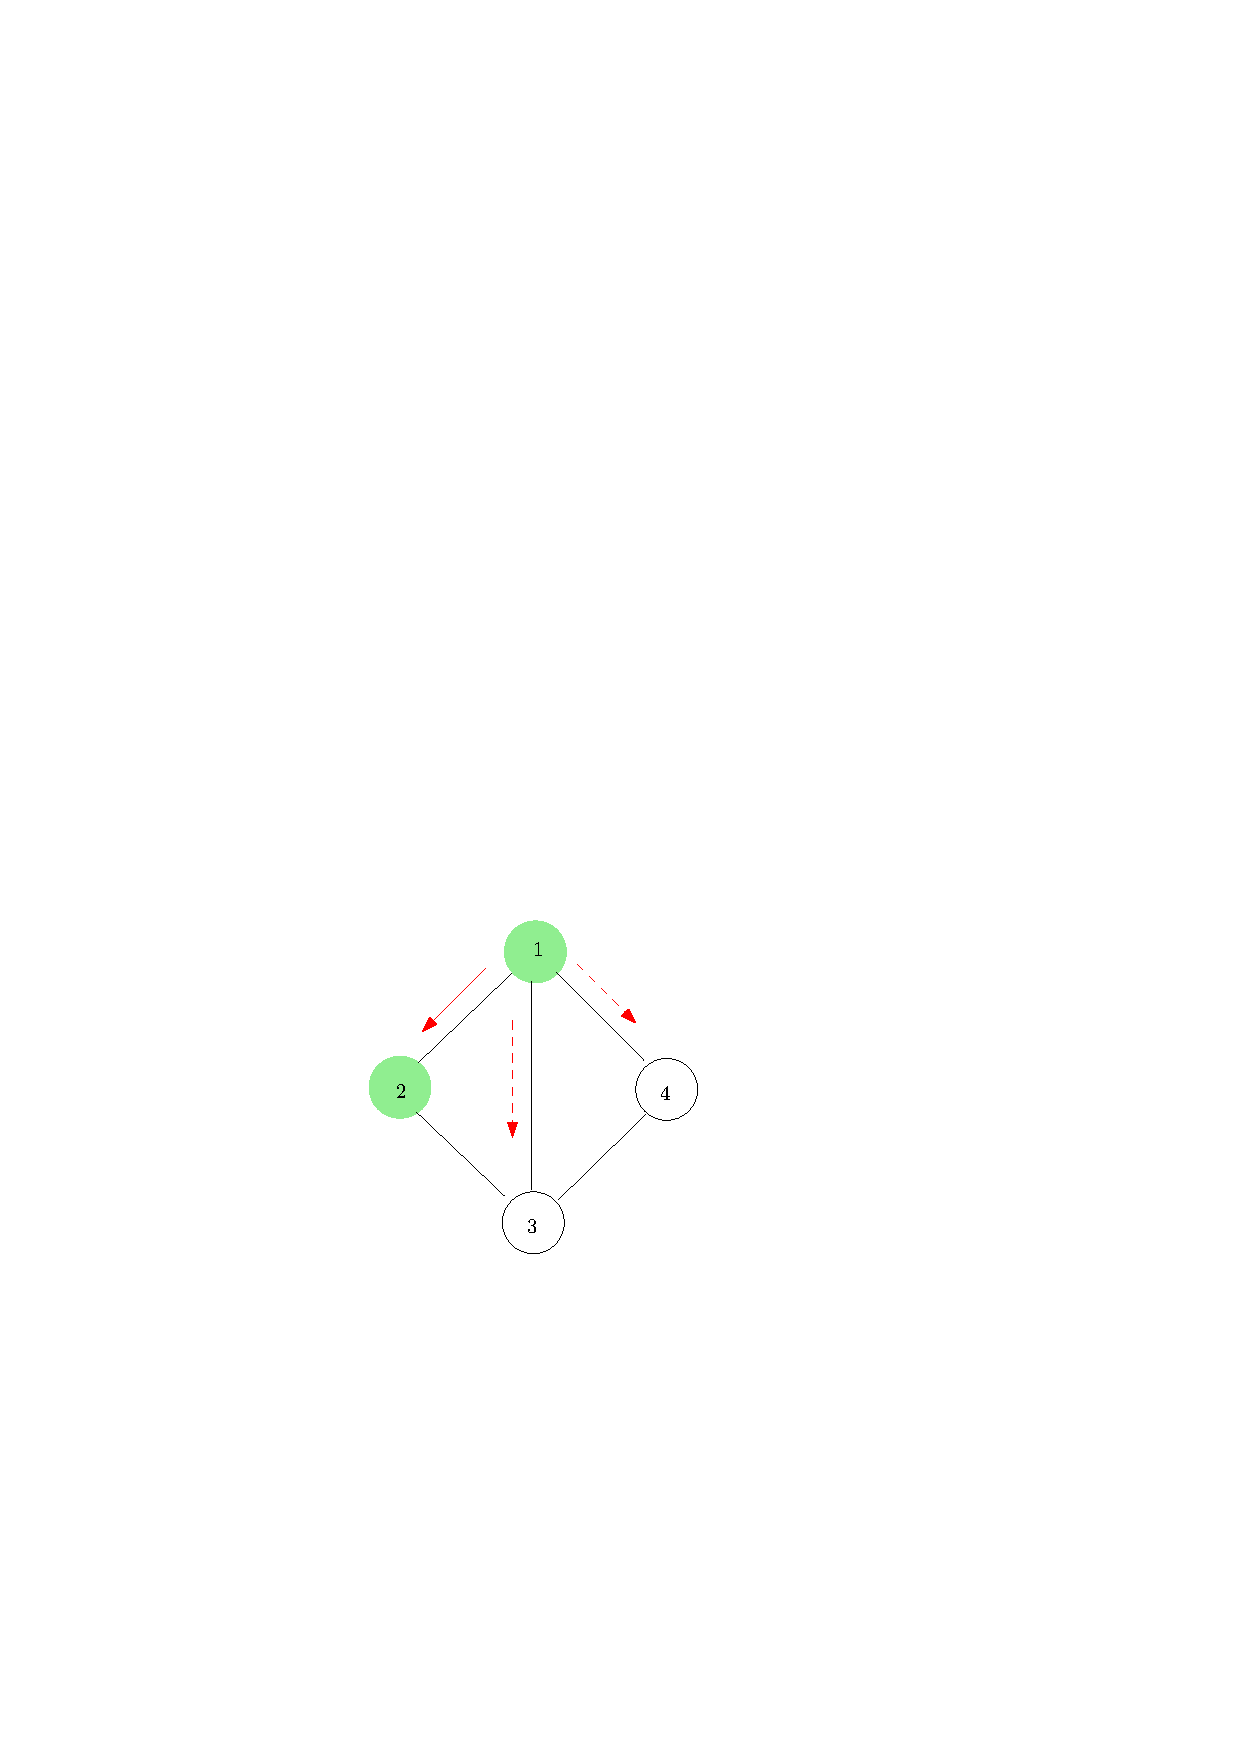
\includegraphics[width=0.32\textwidth]{chapters/background/images/echo/async/notext_f0_1.pdf}}
    \subcaptionbox{Round Two}{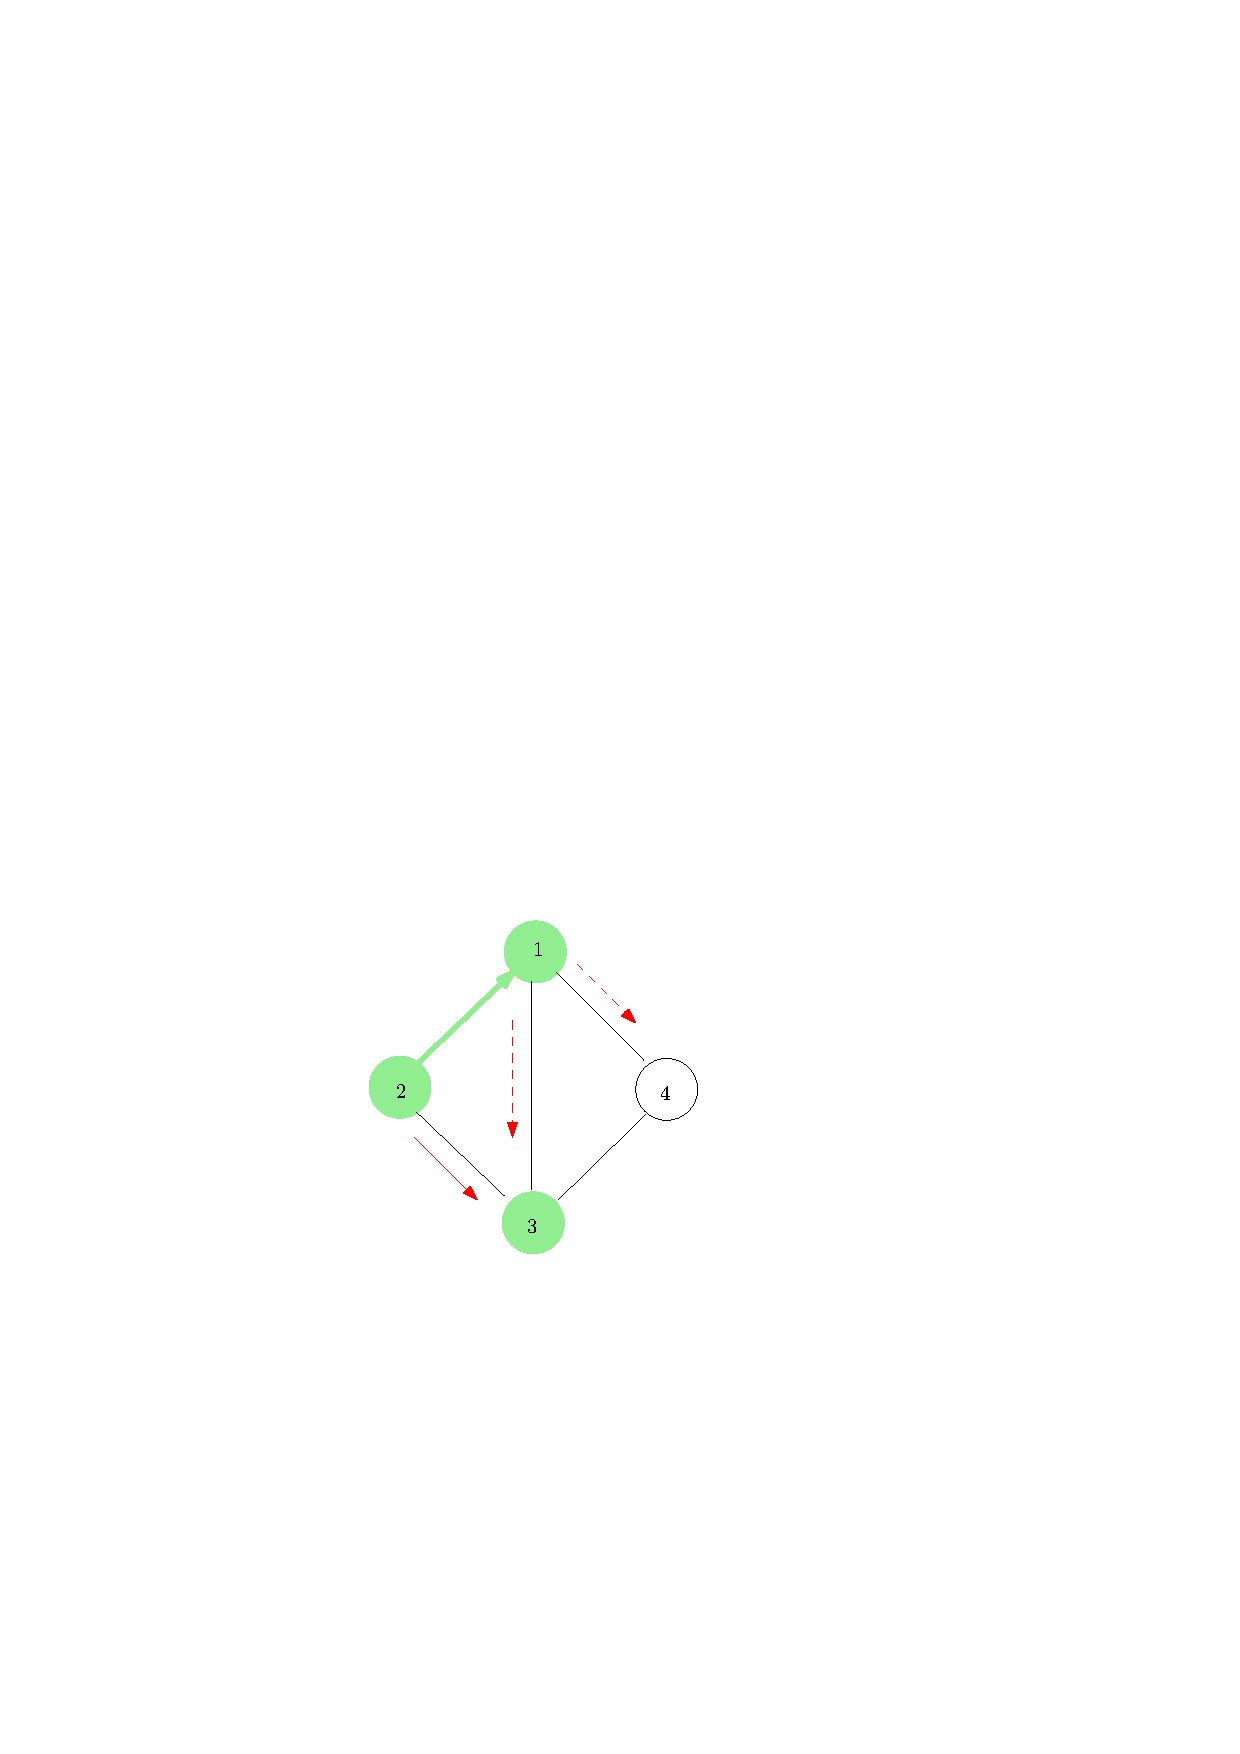
\includegraphics[width=0.32\textwidth]{chapters/background/images/echo/async/notext_f0_2.pdf}}
    \subcaptionbox{Round Three\label{fig:back:echoasync:3}}{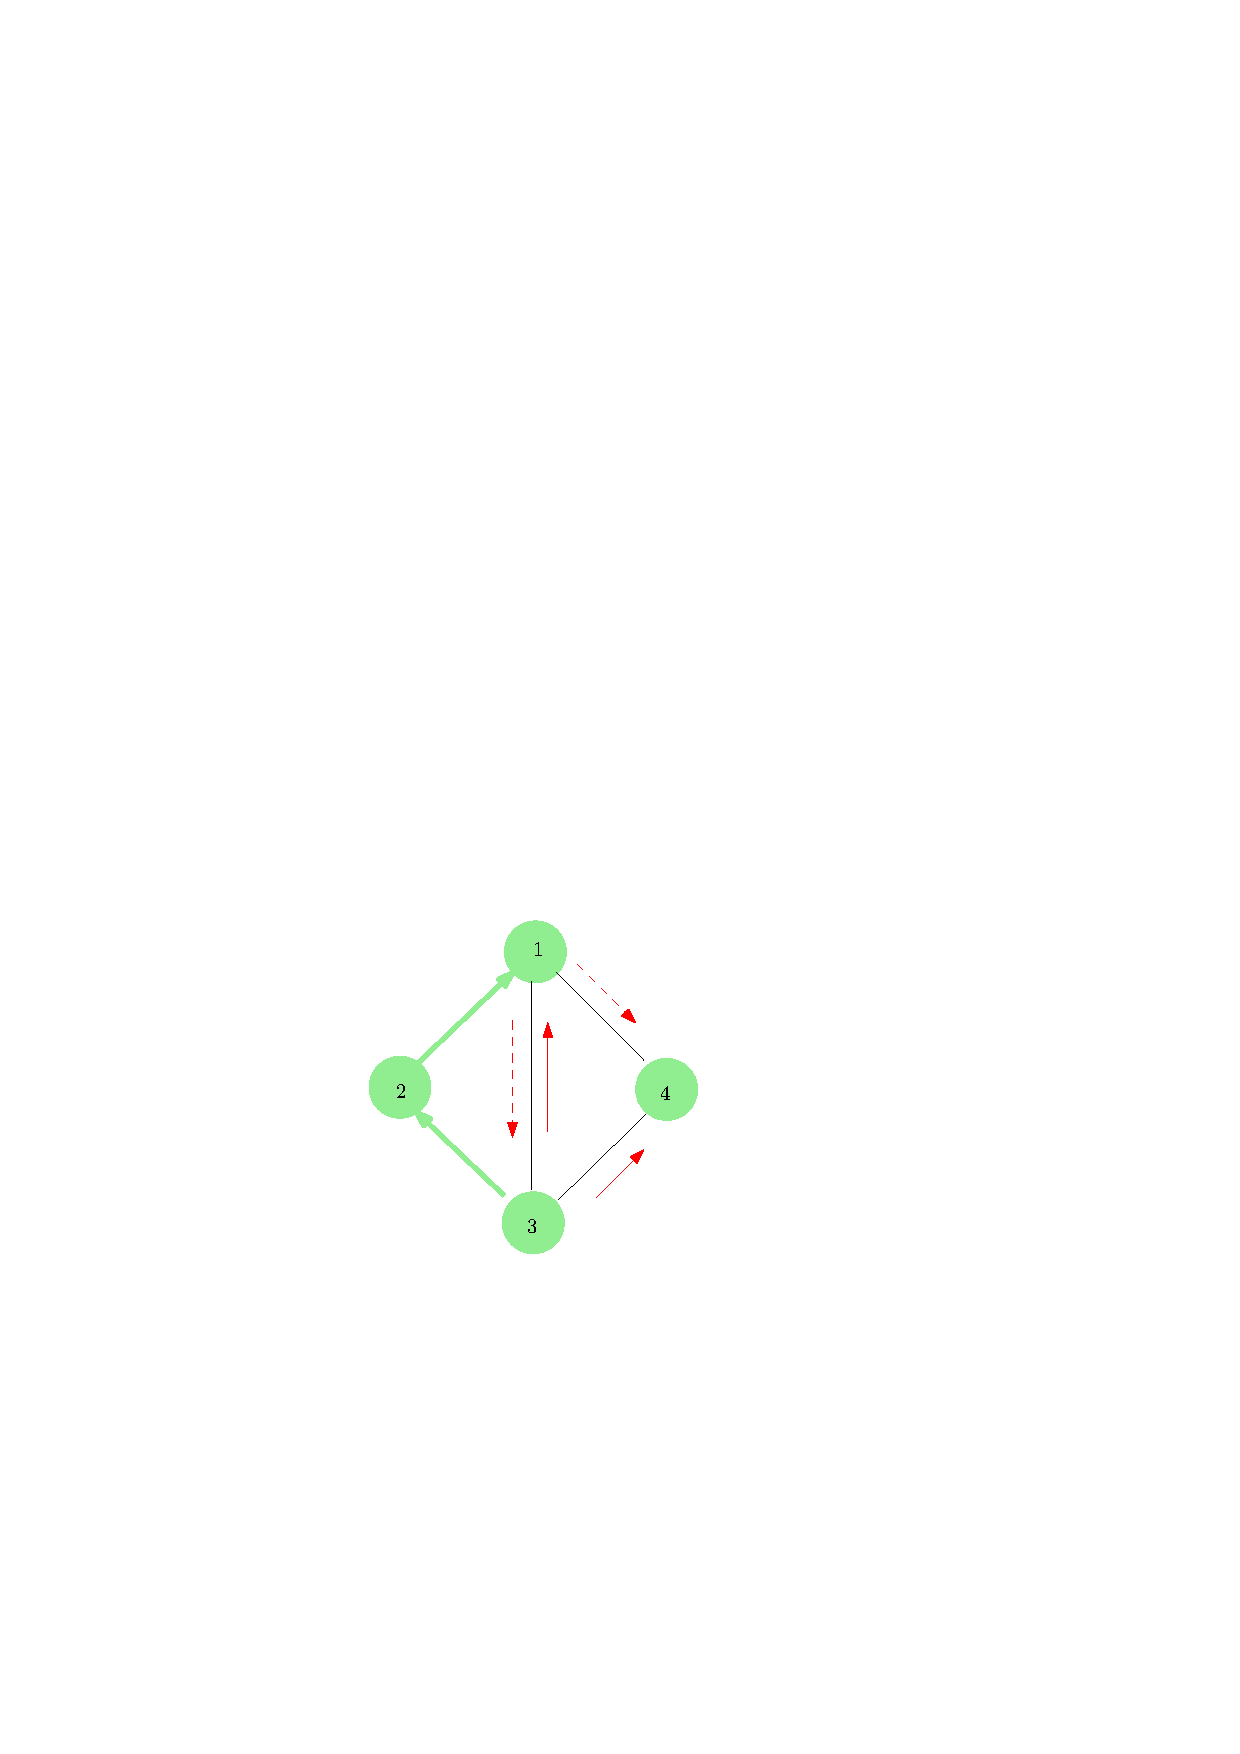
\includegraphics[width=0.32\textwidth]{chapters/background/images/echo/async/notext_f0_3.pdf}}
    \subcaptionbox{Round Four}{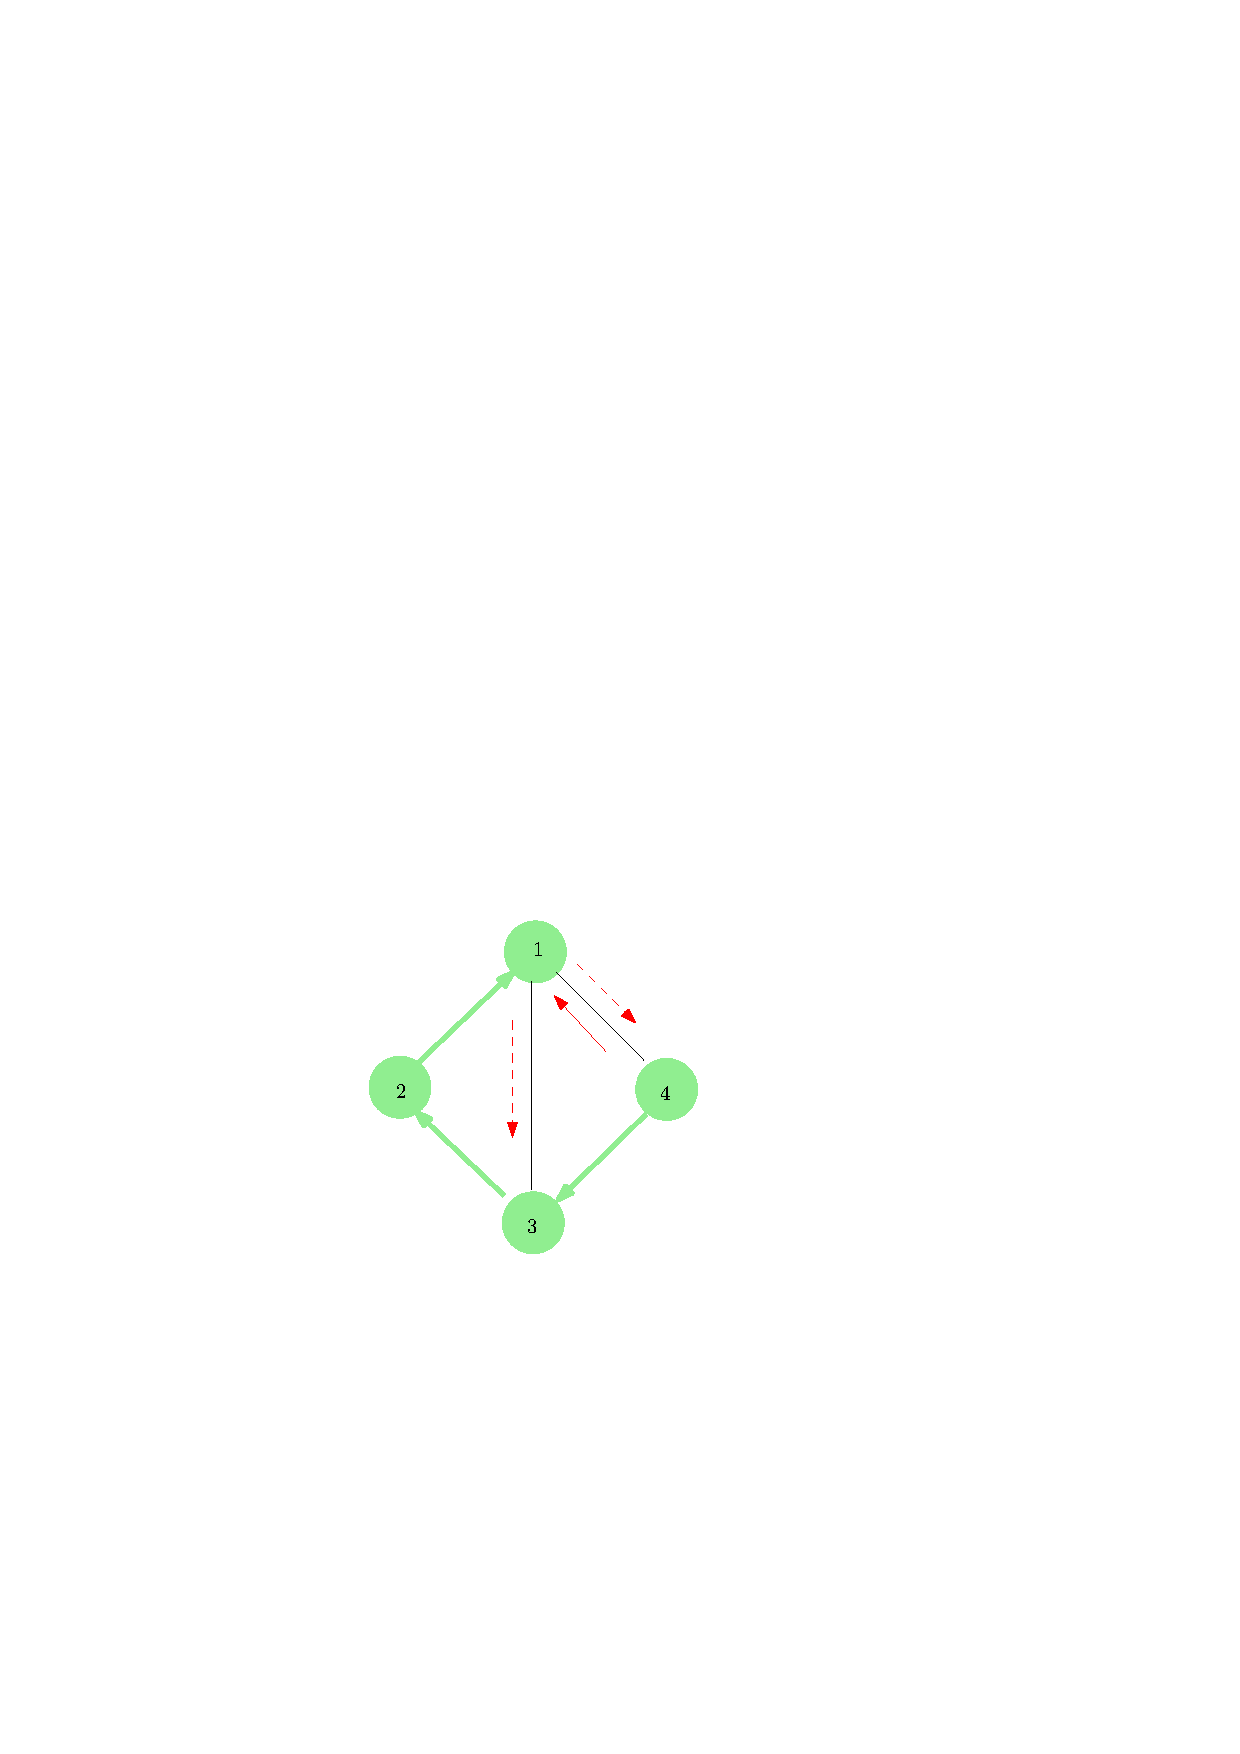
\includegraphics[width=0.32\textwidth]{chapters/background/images/echo/async/notext_f0_4.pdf}}
    \subcaptionbox{Round Five}{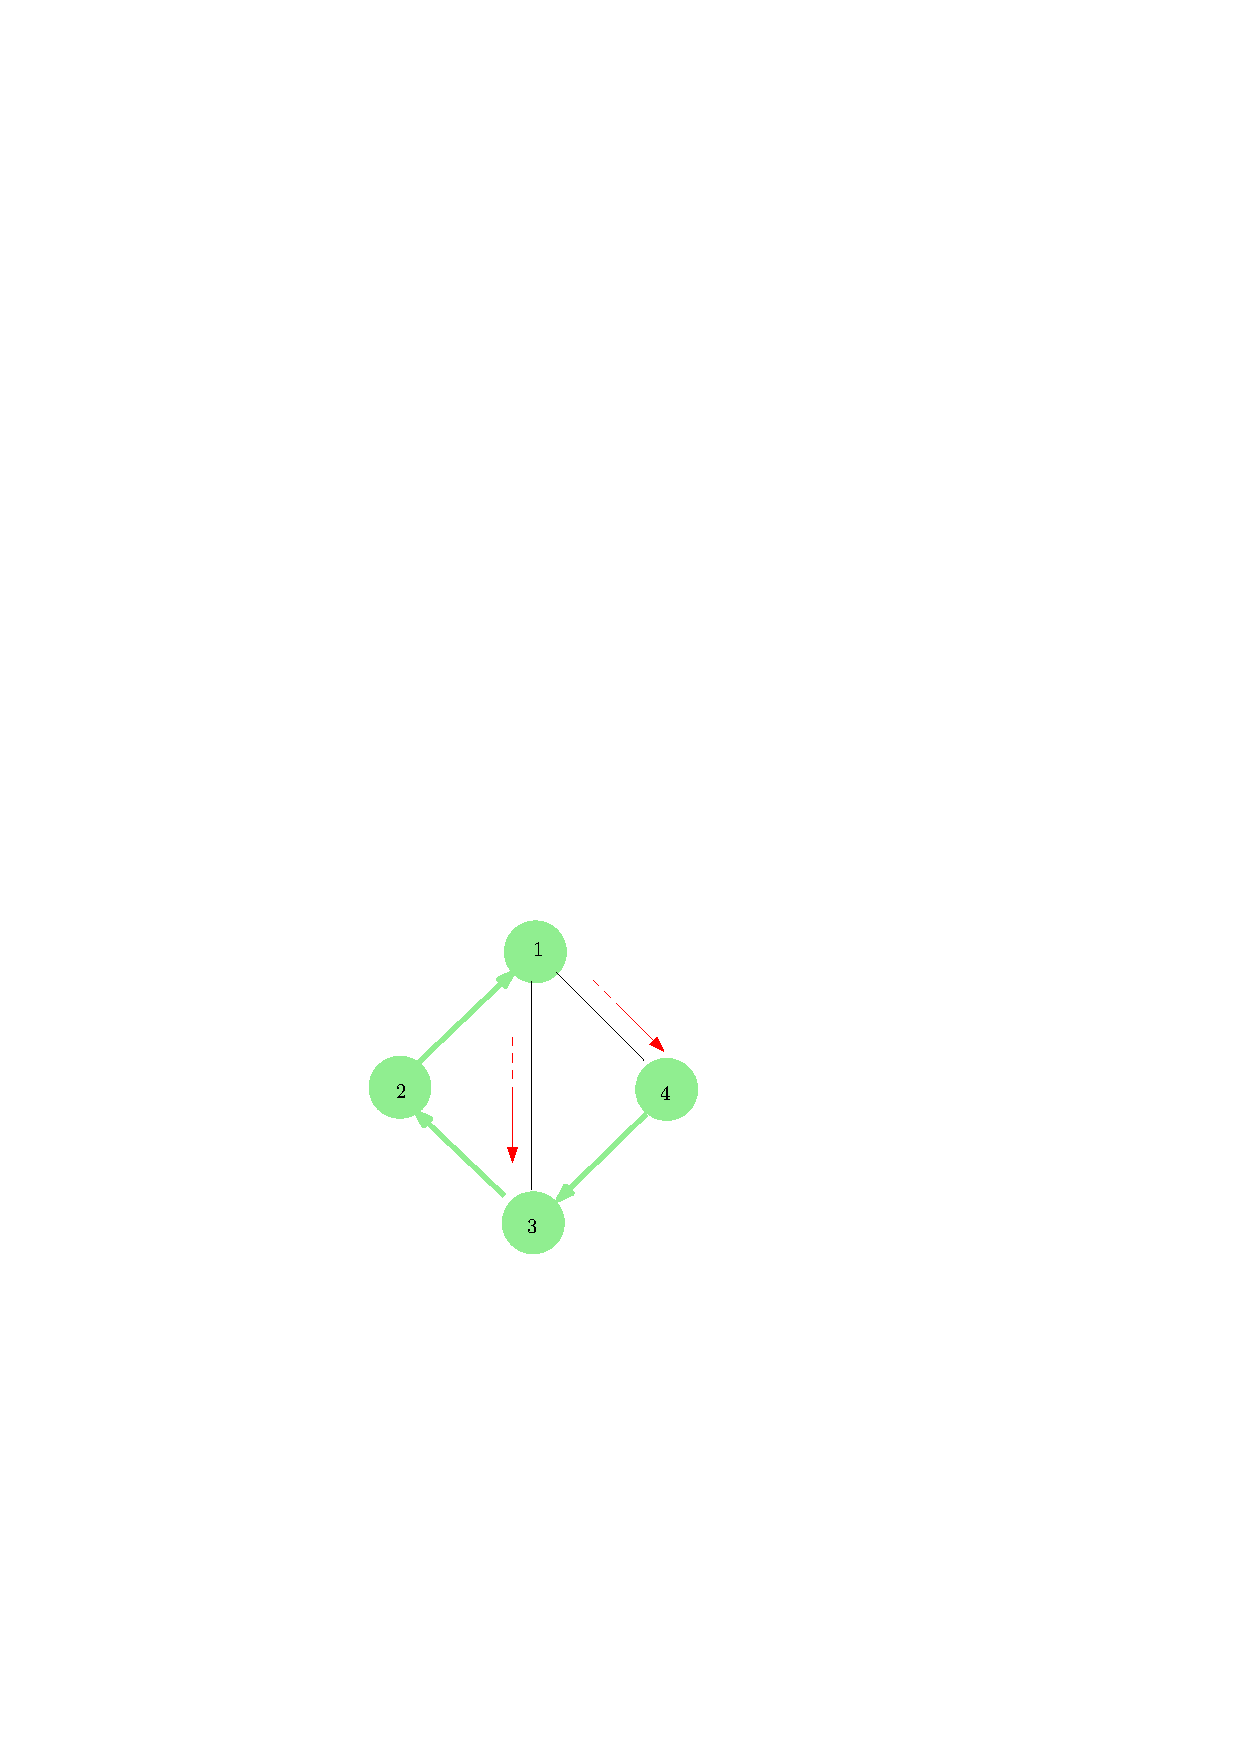
\includegraphics[width=0.32\textwidth]{chapters/background/images/echo/async/notext_f0_5.pdf}}
    \subcaptionbox{Round Six}{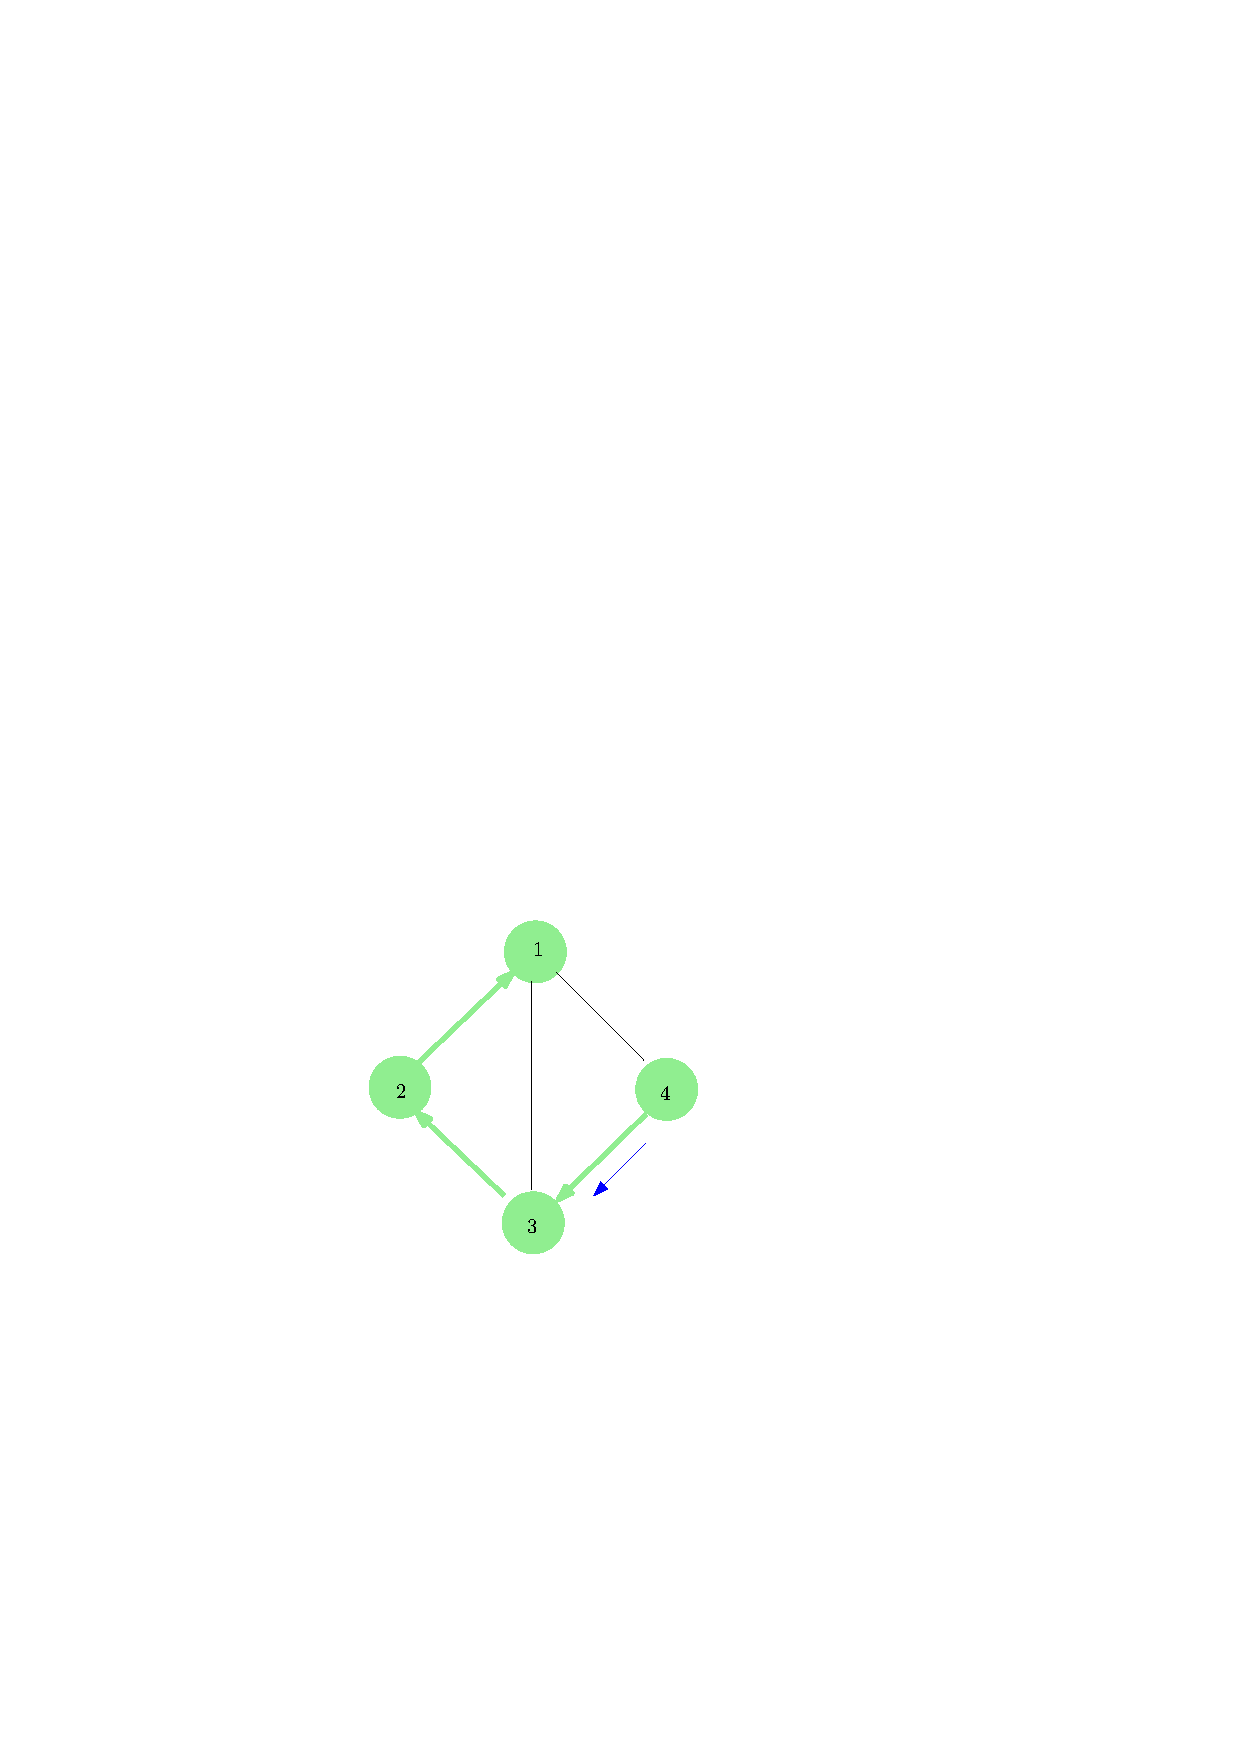
\includegraphics[width=0.32\textwidth]{chapters/background/images/echo/async/notext_f0_6.pdf}}
    \subcaptionbox{Round Seven}{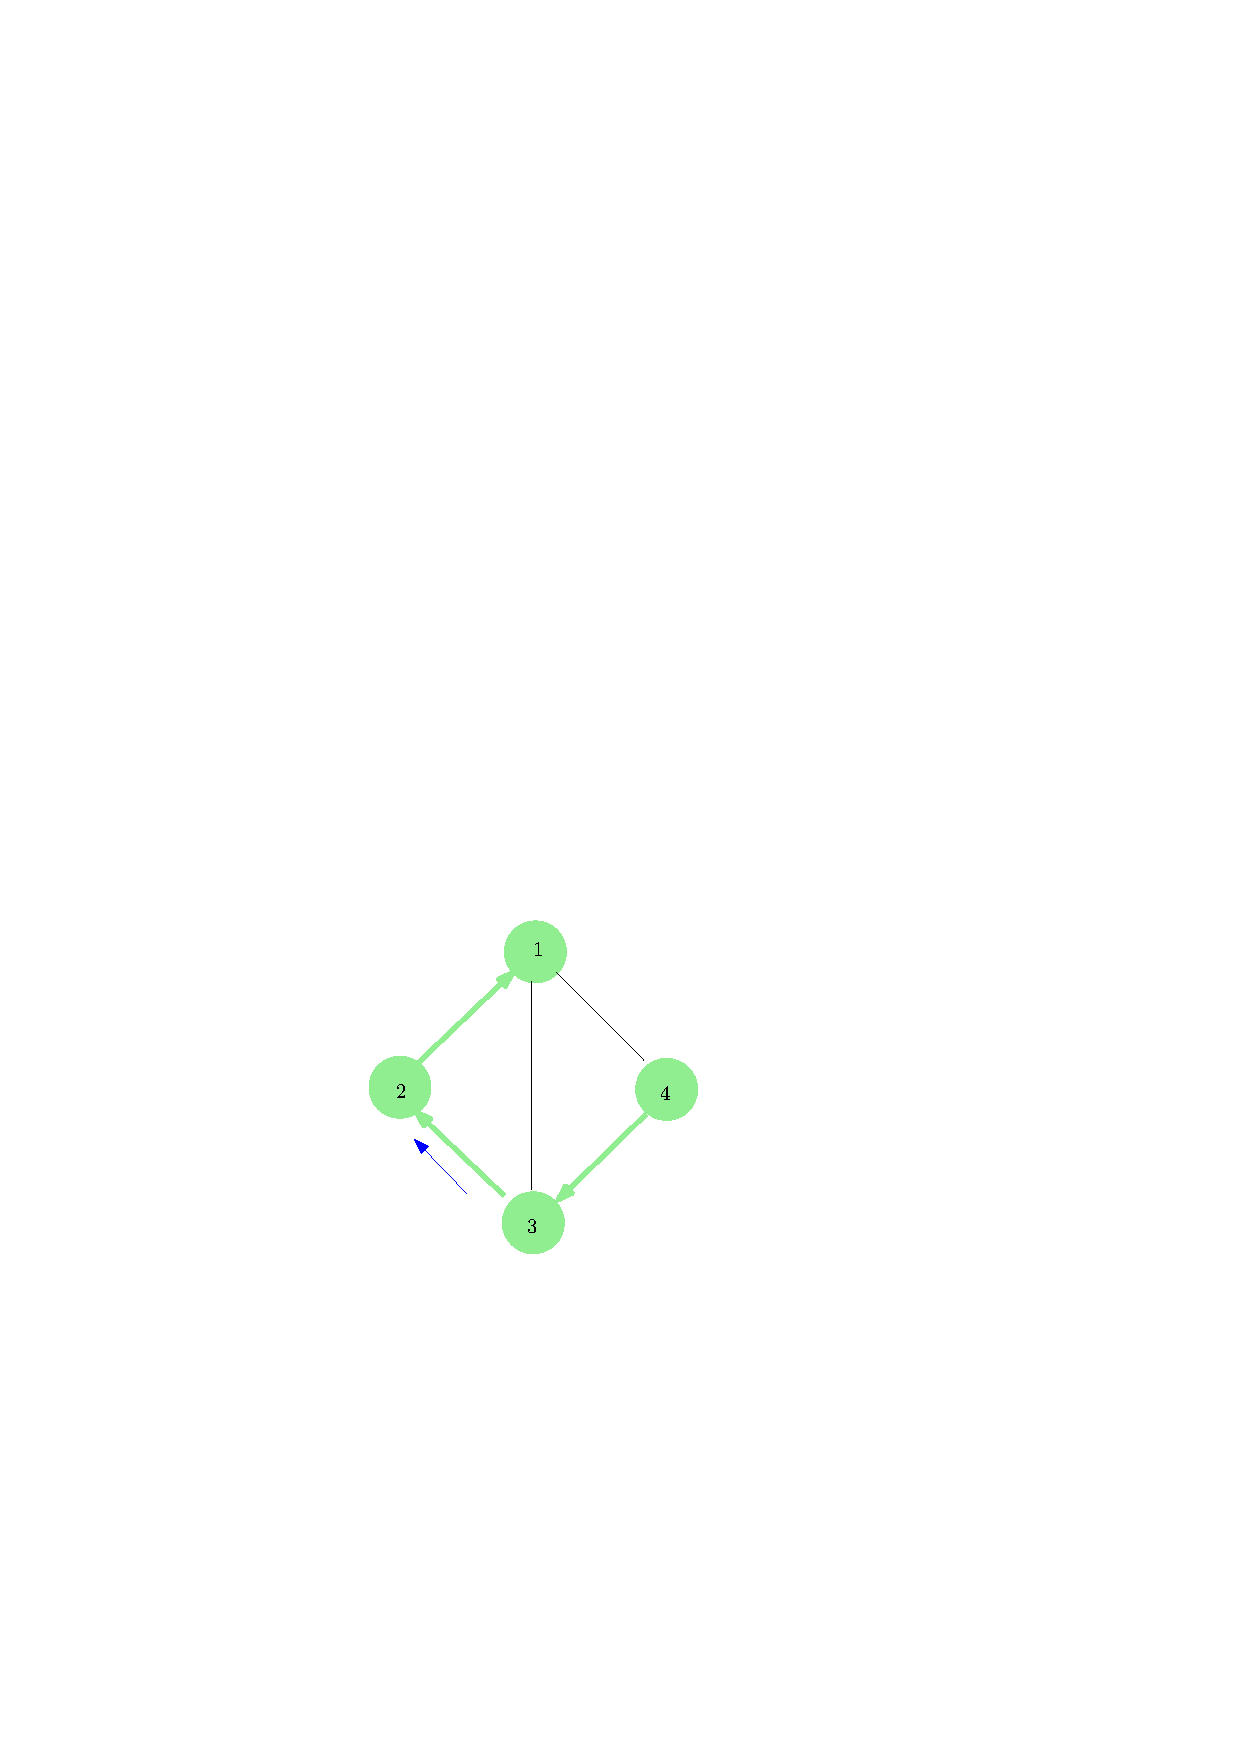
\includegraphics[width=0.32\textwidth]{chapters/background/images/echo/async/notext_f0_7.pdf}}
    \subcaptionbox{Round Eight}{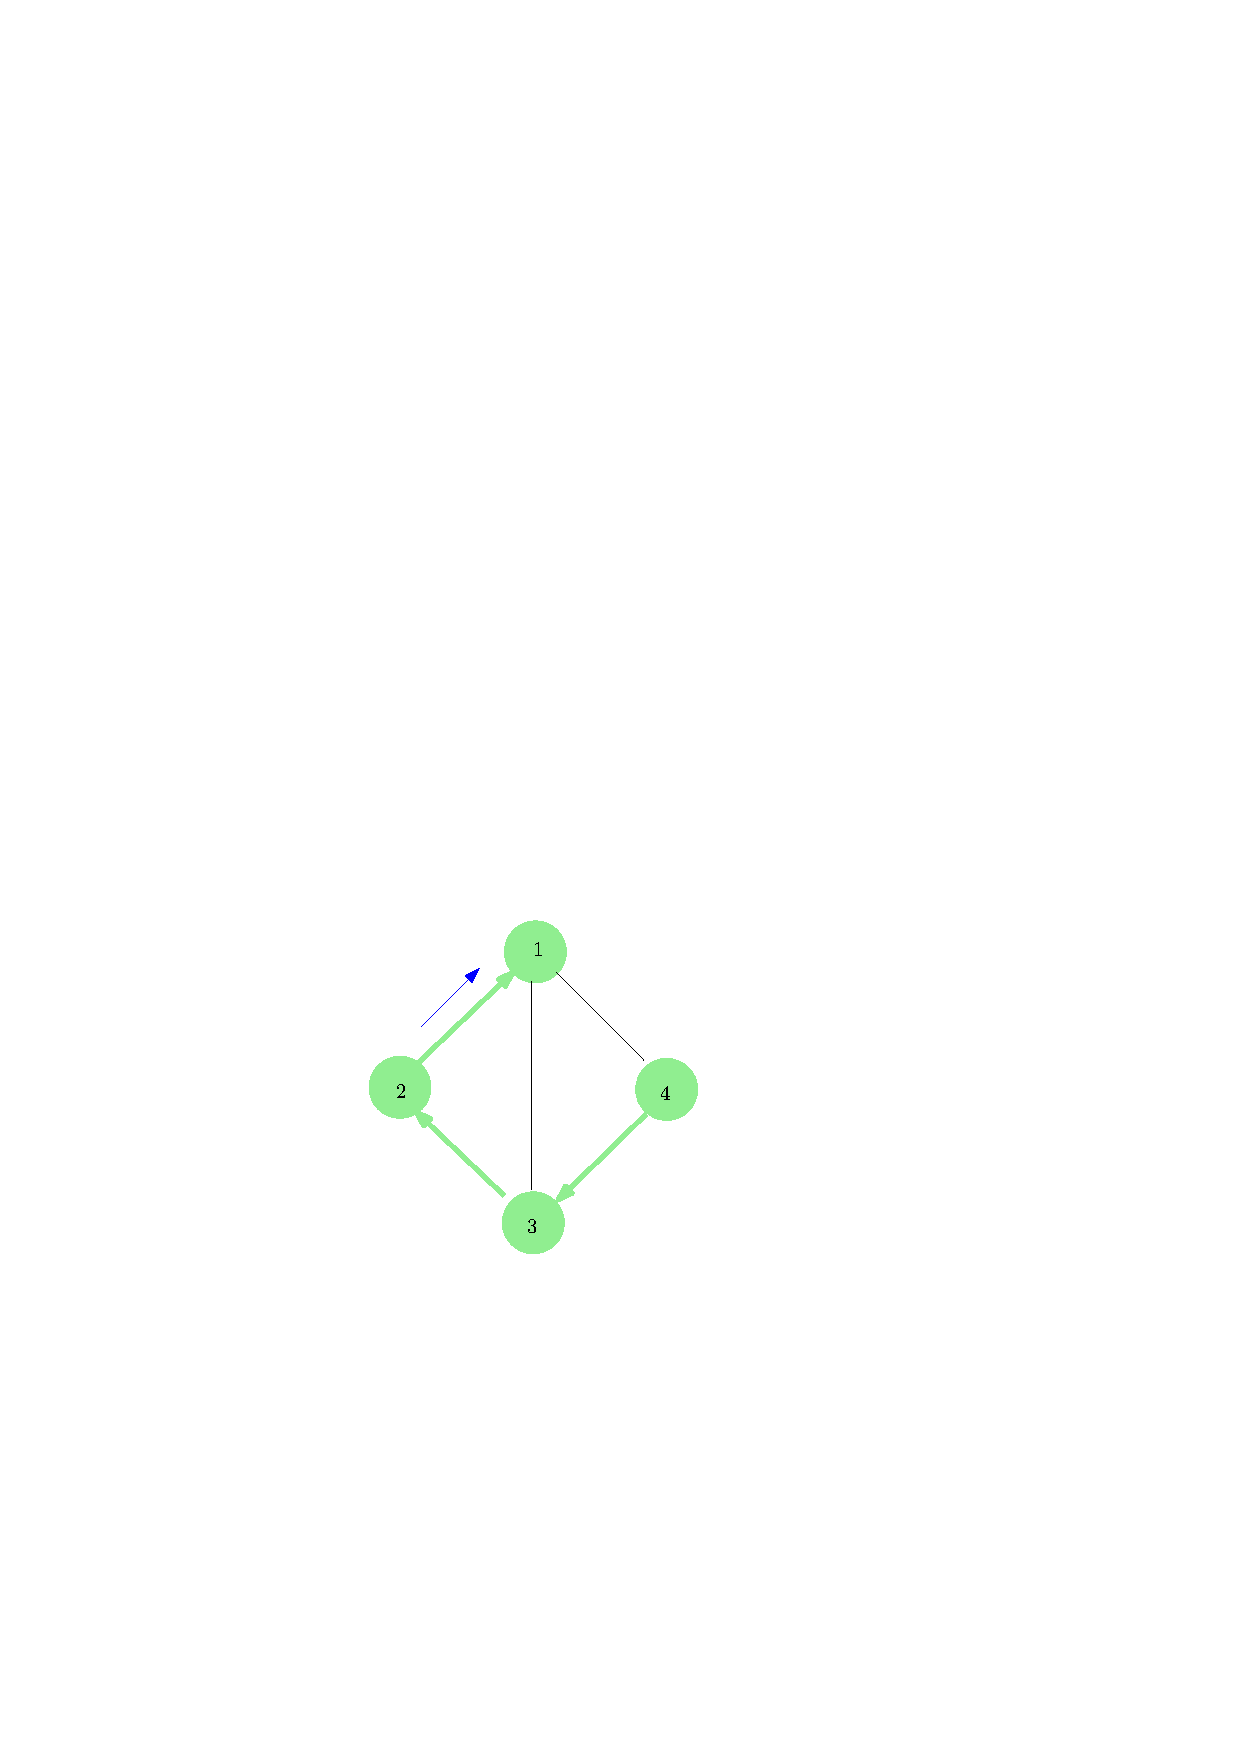
\includegraphics[width=0.32\textwidth]{chapters/background/images/echo/async/notext_f0_8.pdf}}
    \caption[Progression of the asynchronous \textsf{echo} algorithm]{Progression of the asynchronous \textsf{echo} algorithm, starting from round zero before any messages are sent.  Arrows in red mean broadcast messages, while arrows in blue mean convergecast messages.  Despite node 1 being the initiator node, node 4 considers node 3 to be its parent because it first receives a broadcast message from node 3.}
    \label{fig:back:echoasync}
\end{figure}

In the synchronous case, all messages sent out are received simultaneously, and all nodes proceed through their rounds together.  In the asynchronous case, however, messages may arrive at arbitrary times, and nodes proceed through their rounds entirely independently of one another.  The round numbers in the figure mark the point where at least one message has been received by a node.  The nodes react to messages as they arrive, and might do nothing for a time while other nodes are working if no new messages arrive during that time.  Under the asynchronous model, depending on communications topology and speeds, it is possible for the first broadcast message to reach a process to have followed a less direct route from the initiator than otherwise might be possible.  Exactly this is seen in \cref{fig:back:echoasync:3}, where node 4 first receives a message from node 3 (and thus marks node 3 as its parent), despite a direct connection to the initiator, node 1.
\section{\label{sec:back:cml}\glsfmtlong{cml-glossary}}

While parallelism is often the best (perhaps only) way to achieve improvements in execution time for different algorithms once an efficient sequential implementation has been created, it is a notoriously challenging affair \cite{Shun2017}.  When working at the level of directly manipulating threads, such as using the pthreads found in POSIX-compliant operating systems, programmers are exposed to a high level of risk of inadvertently introducing concurrency bugs, such as data races, deadlocks and livelocks.  A panoply of approaches to overcoming this challenge, both theoretical and practical, have been proposed and developed over the years, with varying degrees of success, \eg{} \cite{Boyapati2002,Bocq2012,Seinstra2004}.  Many, perhaps most, large-scale programming languages that use a runtime include some form of parallelism simplification within their standard libraries, \eg{} the Executor system in Java \cite[Ch. 4]{Fernandez2012}, and Swift \& Objective-C's Grand Central Dispatch \cite{Maskrey2018}.

Most simplifications fairly directly target either data-parallelism by simultaneously applying the same operation over multiple elements in arrays, \eg{} SIMD instructions in CPUs \cite{Hughes2015}; or task-parallelism by making provisions for the fork-join model \cite{McCool2012}.  These simplifications can be very useful, but not all instances of parallelism fit neatly into their models.  Algorithms that are well-modelled by the \Gls{csp} and \Gls{actor} models, such as those explicitly centred around concepts of message passing, are not necessarily easy to express using either SIMD or fork-join instructions.

\Gls{cml} \cite{Reppy1991,Panangaden1997} is an approach to concurrent programming originally developed by John Reppy (based on his earlier `Pegasus Meta-Language' \cite{Reppy1988}).  \Gls{cml} was created to provide a framework for creating concurrent programs with synchronous communications on single-core machines,\footnote{In fact, the original implementation \emph{relied} on the fact that the processor was single-core under-the-covers.} and was later extended to permit parallelism \cite{Reppy2009a}.  It was created originally as a library in Standard ML of New Jersey (where ML refers to the earlier programming language \textit{Meta Language}), whence the ML part of the name, but its concepts have subsequently appeared elsewhere.  The basic concept of communicating via channels has experienced a renaissance in recent years, likely due at least in part to its inclusion as a core feature of Go \cite{Meyerson2014}, but \gls{cml} has a more advanced system that Go (at the time of writing) does not fully support.

\Gls{cml} is designed to avoid many of the problems with concurrency that arise in traditional sequential programming, where the use of locks, mutexes and semaphores etc. are frequently required, and often lead to the potential introduction of problems such live-/deadlocks, data races and extreme resource contention.  This is achieved by changing the approach to concurrent programming to one of logically separate, internally sequential processing elements that share data as required by `passing messages'\footnote{This is the logical concept, but there is not strictly any specific required software implementation.} between themselves.  In \gls{cml}, these logical processing elements are referred to as threads, and they exchange messages over channels \emph{synchronously} (called \emph{rendezvous}), \ie{} there is a temporal overlap between one thread offering to send, and another to receive, over the same channel, and the first to offer blocks until the second makes its offer.  When two processes are offering appropriately on either side of an exchange, rendezvous takes place.

Reppy describes a concurrent program as one that supports multiple sequential sub-programs conceptually executing in parallel separately, but interacting through shared resources to achieve a common goal.  \Gls{cml} is concerned with the scenario where said interactions are explicit, and in order to facilitate that \enquote{\gls{cml} takes the unique approach of supporting \emph{higher-order concurrent programming}} (emphasis Reppy's), whereby communication and synchronisation are made into first-class members of the language, similar to how functional programming languages made functions into first-class members of themselves \cite[Preface]{Reppy2007}.

\begin{anfxerror}{Expand this?}
Describe more of how \gls{cml} works?  Is there not something in the gcol chapter that can be shifted into here, at least?
\end{anfxerror}
\section{\label{sec:back:mc}\Glsfmtname{mc}/\glsfmtname{ps}}

\emph{\Gls{mc}}, also known as \emph{\gls{ps}} (the two terms are generally used interchangeably), is a bio-inspired model of computing created by Gheorghe Păun in the late 1990s \cite{tPaun98a,Paun2000}.  It was originally conceived of by considering the process of chemical reactions and exchanges that occur inside living biological cells and the membranes within, and regarding this process as a form of computation.  \Gls{mc} was identified in 2016 by the National Research Council of Canada as \textcquote[][p. 17]{Wiseman2016}{a rigorous and comprehensive framework that provides a parallel distributed framework with flexible evolution rules.}

\citeauthor{Paun2002} describes \gls{mc} as:
\blockcquote[][p.~VII]{Paun2002}{Membrane computing is a branch of natural computing which abstracts from the structure and the functioning of living cells. In the basic model, the membrane systems -- also called P systems -- are distributed parallel computing devices, processing multisets of objects, synchronously, in the compartments delimited by a membrane structure. The objects, which correspond to chemicals evolving in the compartments of a cell, can also pass through membranes. The membranes form a hierarchical structure --- they can be dissolved, divided, created, and their permeability can be modified. A sequence of transitions between configurations of a system forms a computation. The result of a halting computation is the number of objects present at the end of the computation in a specified membrane, called the output membrane. The objects can also have a structure of their own that can be described by strings over a given alphabet of basic molecules - then the result of a computation is a set of strings.}

\begin{anfxerror}{P systems Diagram?}
Include a copy of the membrane layout diagram from Paun?
\end{anfxerror}

\Gls{ps} works analogously to a typical modern electronic computer, in that the system stores data and processes \& updates those data based on a predefined program, with a view to arriving at a computable answer based on the starting state and any inputs to the system \cite{Paun2002,Paun2010b}.  In classical \gls{ps}, the data are multisets of symbols, representing various chemicals and their quantities.  These are found inside one or more \emph{cells},\footnote{Loosely based on real biological cells.} which (to a certain extent at least) form a hybrid between main memory and the processing units of a computer.  The instructions of the program itself are provided by \emph{rules}, which specify transformations of objects and interactions with the surrounding environment and other membranes or cells.

There are now, broadly, three main families of \gls{ps} variants:  \gls{clps} \cite{Paun2001,Paun2002}, \gls{tlps} \cite{tMaPaPaRo01a,Martin-Vide2003} and \gls{snps} \cite{Ionescu2006}.\footnote{Several other variants have been created, but most are used infrequently, if ever.  Most recent work in \gls{mc} has focused on sub-variants of \gls{clps}, \gls{tlps}, \gls{snps} and \gls{cps}.}  \Gls{clps} is the direct descendant of the original classical \gls{ps}, and sees objects compartmented into \emph{membranes}, which are arranged in a graphical tree structure with the outermost \emph{skin} membrane -- which separates the cell from its environment -- as the root of the tree.  In most variants, objects can evolve inside a membrane, but also be communicated between membranes (and the environment).  Furthermore, membranes can \emph{divide} or \emph{dissolve} themselves, and may have one or more special properties, such as \emph{polarization} \cite{Paun1999a}.

On the other hand, \gls{tlps} and \gls{snps} both arrange their computing compartments -- named \emph{cells} or \emph{neurons}, respectively -- as nodes in arbitrary digraphs, with the edges between them representing connecting channels or synapses.  Whereas \gls{clps} emphasises the evolution of multisets of objects inside membranes of a given cell, \gls{tlps} and \gls{snps} emphasise communication between separate cells/neurons, and might not include any capacity for internal evolution inside cells.  If new objects are required, they are imported via communication with the environment, which possesses an unlimited number of all objects but has no rules of its own.

While \gls{tlps} have arbitrary alphabets, only one object is used in \gls{snps}, the \emph{spike}.  This means that \gls{tlps} are frequently much like \gls{clps} in that they have custom objects for each purpose, with the key difference (usually) being in the arrangement of the compartments/membranes/cells relative to each other and the choice between the two motivated primarily by which one better fits the computation to be modelled.

Conversely, \gls{snps} represent everything through the use of differing quantities of the spike, kept in different neurons.  This means that it can be more complex to model certain problems, but also arguably means that \gls{snps} are, \textit{prima facie}, closer to Lambda Calculus \cite{Barendregt1984} and Church Numerals (see \eg{} \cite{Koopman2014,Hinze2005}), as well as Register Machines (see \eg{} \cite{Korec1996}) (and indeed Register Machines have been simulated with \gls{snps} \cite{Pan2010}).  All three main types of \gls{ps}, in some form, have been proven Turing-universal though \cite{Bernardini2005,Chen2008,Freund2005}, so all three should be capable of expressing the same computations in different forms.  Furthermore, because \gls{snps} can be easily represented numerically, they lend themselves well to vector/matrix representations \cite{Zeng2010,Martinez-del-Amor2021,Gheorghe2021,Hu2016}.  This means that, potentially, \gls{snps} implementations can take advantage of high-performance techniques such as directly using \gls{blas} \& \gls{lapack} and/or \glspl{gpu} \cite{Aboy2019}.

Arguably, the most noteworthy and important aspects of \gls{ps} models are that:
\begin{inparaenum}[(i)]
\item They have no space limit.  That is, they contain an unbounded number of cells, objects and membranes;
\item Usually, across all cells and membranes, all rules that can be applied are applied, as many times as possible given the current number of objects available.
\end{inparaenum}
These two features mean that \gls{ps} have unbounded space and processing capacity, which can be used to solve traditionally computationally difficult problems relatively quickly \cite{Sosik2003,Jimenez2003,Paun1999a,Henderson2020}.  Most of these solutions, however, rely on trading time complexity for space complexity.  While this works in the theoretical framework, electronic simulations of the systems do not have access to unlimited instantaneous memory space, meaning many of the fast solutions are impractical with current real-world computers, \eg{} \cite{Cooper2019,Cooper2019a} \fxnote[inline]{[refs]} (see further \vref{sec:psystemsuses}).

\citeauthor{Valencia-Cabrera2019} said of this:
\blockcquote[][p.~213]{Valencia-Cabrera2019}{We do not know if we will have those machines able to solve NP-complete problems in polynomial time, in many cases even linear time, but \textins{that does} not necessarily mean we will have to wait until that moment in biochemical technology to find some relevant use of P systems. As Babbage kept working on his ideas, not simply waiting until the precise moment when Turing, Von Neumann, and their contemporaries witnessed the first electronic computers based on similar principles, membrane computing must keep moving, finding new ways to provide a step further.}

Nevertheless, modelling a problem in \gls{mc} can lead to new insights or improved formulations of solutions, as occurs in \cref{chap:nmp}.  For example, in \cite{GimelFarb2013a} (building on \cite{Gimelfarb2011}) \citeauthor{GimelFarb2013a} describe how formulating Symmetric Dynamic Programming \gls{sm} in terms of \gls{ps} led to finding a bug in the implementation, \textcquote[][p.~24]{GimelFarb2013a}{but also (and what is much more important) refactor this algorithm, based on our cell structure.  The result is a more robust and flexible version, which allows us to fine tune its parameters and enhance its capabilities, without rewriting it from scratch.}  Furthermore, as reported in \cite{Nicolescu2014b}, this exercise led directly to the creation of a new \gls{sm} algorithm, Concurrent Propagation \cite{Gimelfarb2012}.  \citeauthor{Pang2018} \cite{Pang2018} also claim significant benefits from modelling certain problems in a novel variant of \gls{enps} \cite{Pavel2010}, but it is unclear how much of the stated benefit compared to their baseline implementation arises instead from the use of a \gls{gpu}.

\subsection{Objects, Rules and Steps}
All known \gls{ps} types fundamentally operate on a similar basis:  One or more sets of rules -- \emph{\gls{ruleset}} -- are defined, describing how the \emph{objects} present in the system's compartments change at each \emph{step}.  As mentioned above, the objects are usually multisets of arbitrary symbolic \emph{atoms}, with the exceptions of \gls{snps} which uses the spike as its only symbol, and Numerical \gls{ps}, which uses ordinary numbers in place of atoms.  Certain systems may introduce other object types as required.

\Gls{ps} types normally operate synchronously and assume the presence of a global clock.  At each clock ``tick'', every compartment compares its extant objects and its \emph{evolution rules}, determines which rules are applicable given the current objects, and then deletes the objects used in the rules, replacing them with new ones as the rules dictate.  This process comprises a step.  The progressive execution of the system's rules over multiple steps is referred to as the system's evolution.

All \gls{ps} evolve, and therefore all types have evolution rules (though they may not be referred to as such).  Other types of rules are possible, including: \emph{dissolution} and \emph{division} rules in \gls{clps} and \gls{tlps}, where membranes either dissolve and release their objects into the their parent membrane, or replicate themselves (essentially performing mitosis) and distribute their contents among the new membranes; \emph{forgetting} rules in \gls{snps} whereby one or more copies of the spike are removed from a given neuron; or, splicing rules in Splicing \Gls{ps}\footnote{Particularly notable for working over strings of an alphabet, instead of multisets.} \cite[Ch.~8]{Paun2010b}.

All rules use the same basic model.  At the start of a step, they check if the necessary pre-conditions for the rule are met.  If they are, then any changes to the state of the system specified by the rule occur.  It is common for rules to remove or delete some objects in the relevant compartment, and instantiate new ones.  It is typically assumed that all objects are deleted or created instantaneously at the last moment of the rules' execution.

Generally, rules are specified in the form \textsc{\gls{lhs}} \(\rightarrow\) \textsc{\gls{rhs}}, where objects to be removed (the presence of which are therefore a precondition) are written in the \gls{lhs} and the objects to be created are written in the \gls{rhs}.  Unless otherwise specified, it is typically assumed that all rules which can be applied at a given step are applied.

\subsubsection{Weak Priority Order}

Many, perhaps most, types of \gls{ps} \glspl{ruleset} use a \emph{weak-priority} ordering.  This means that some rules will be tested for applicability ahead of others, on some priority basis, but earlier applicable rules only prevent later applicable rules from being applied if there is a conflict between the two.  The most common way that this conflict can arise is by two rules trying to use the same pre-existing object in the compartment.

Generally speaking, an individual rule will select for use one or more copies of one or more objects the multiset.  At the end of the rule's application, these objects are deleted and replaced with any new ones the rule specifies.  Since the rule will delete the chosen objects, it would not make sense for another rule to be able also to use and then delete the same objects.  Therefore, the first rule to select (or take hold of or seize \etc{}) a given object prevents any other rule from using it too, and thus the first rule has priority over later rules.

The typical method of defining rules' priority is to use \emph{top-down} ordering.  This simply means that the rules presented first in a \gls{ruleset} have priority over those rules presented further down.  The basic process to determine which rules to apply is therefore a sequential one.  Starting with the first rule, and proceeding with each successive rule in turn, test if the rule is applicable at all.  If it is, set it to be applied during the step as many times as possible depending on the rule, the objects present, and the run-time mode (see \eg{} \cref{sec:cps:applicationmodes} for a discussion of this in relation to \gls{cps}).

Any objects now set to be deleted by a previous rule are then unavailable to a later rule, but if there are sufficient remaining objects for that rule to apply, it still may, giving a \emph{weak} priority to the earlier rules.  The application of an earlier rule does not guarantee that a later rule will not apply, but the earlier rule takes precedence in the case of a conflict.  Furthermore, some \gls{ps} variants, \gls{cps} included, use states on their compartments (or the system as a whole).  In this case, rules will usually state a necessary starting state, and an ending state to which the rule transitions the system.  The first such rule to apply dictates the ending state of the compartment (or system) at the end of the step.  Rules with a lower priority may then only be applied if they have the same requisite ending state.

%%%%%%%%%%%%%%%%%%%%%%%%%%%%%%%%%%

\subsection{Computer Representations and Simulations of \glsfmtname{ps}}

\subsubsection{\Adhoc{} and General Simulations}
There are arguably two main approaches to simulating \gls{ps}:
\begin{inparaenum}[a)]
\item ``\Adhoc{}'' simulations, where a separate program is written specifically for a given type of problem and its \gls{ps} solution; and
\item ``General'' simulations, where a separate simulation engine capable of simulating one or more types of \glspl{ps} is created independent of a given problem, and is supplied problem-specific configurations.  The engine uses the configuration to initialise the simulated system, and works through the problem from there.
\end{inparaenum}

The main advantage of the \adhoc{} style is the ability to adjust and optimise the simulation's implementation to suit the \gls{ps} variant used, and the problem at hand.  In general, \adhoc{} simulations would be expected to require less resources to find the answer, \eg{} running faster and/or using less memory.  The major disadvantage of the \adhoc{} approach is that a new simulation must be developed for each problem studied, requiring more time and greater levels of technical skill while reducing flexibility.  The main advantages of the general approach are greater flexibility from the produced program -- \ie{} it can simulate more problems -- and a broadening of the people who can experiment with different \gls{ps} variants and problems to those with lower levels of programming expertise.

General simulations permit specialisation and a division of labour, meaning one person can look into new \gls{ps} variants and problems to apply them to, while another person focuses on developing and improving the simulation engine itself.  This is a clear upside, but there is equally a downside: lacking problem-specific knowledge, the general simulations usually do not perform all potential optimisations, meaning that there could be unavoidable upper bounds on the efficiency of a simulation, no matter the specific problem at hand.  Furthermore, general simulations must run inside another program, whereas \adhoc{} simulations can be created as independent, native executables.

Traditionally, this has been an `either/or' problem, where one can take either a wholly \adhoc{} approach or a wholly generalist approach.  \citeauthor{Perez-Hurtado2019} more recently introduced a \gls{ps} ``compiler'' \texttt{pcc} \cite{Perez-Hurtado2019}, which can produce a standalone native executable from a non-programmatic specification of a particular \glspl{ps} --- thus providing a third, middle-ground option.  They say of this compiler: \textquote{the goal of \textins{\texttt{pcc}} is twofold: On the one hand, it purports to be a good assistant for researchers while verifying their designs, even working with experimental models. On the other hand, it provides optimized simulators for real applications, such as robotics or simulation of biological phenomena.}  It was not used in this dissertation, as \texttt{pcc} did not support \gls{cps} at the relevant time, but the idea holds great promise for the future.

%%%%%%%%%%%%%%%%%%%%%%%%

\subsubsection{\label{sec:back:simulators}\Glsfmtname{ps} Simulators}

\citeauthor{Valencia-Cabrera2019} provide a summary of the development of simulators for \Gls{ps} since the field's inception in the late 1990s \cite{Valencia-Cabrera2019}.\footnote{The authors also provide a timeline of practical works in \gls{ps} at \url{https://github.com/RGNC/plingua}.  Some of the software described in this \lcnamecref{sec:back:simulators} is available at \url{http://ppage.psystems.eu/index.php/Software/}.}  Unsurprisingly, most early simulators were \adhoc{} and created for a specific purpose, focusing on one problem domain and simulating one \gls{ps} variant.  Many were intended for formal verification of models as much as they were for practical use \cite{Gutierrez-Naranjo2007}.  These early simulations were written in a wide variety of programming languages, including (comparatively) lesser-used languages such as Haskell, Prolog and LISP.  Notably, \citeauthor{Ciobanu2004} created a simulator specifically for distributed computing, using C++ and \gls{mpi} \cite{Ciobanu2004}.

As the number of \gls{ps} variants defined, and simulations to experiment with them, expanded greatly, it began to make more sense to create general simulators which did not require detailed customisation for every experiment.  A handful of these multi-purpose simulators began to appear, including (among others): PSim \cite{Bianco2007,Bianco2007a}; a transpiler from Systems Biology Markup Language (SBML) to C Language Integrated Production System (CLIPS) \cite{NepomucenoChamorro2005};  and a web-based simulator which also made use of CLIPS \cite{Bonchis2005}.  Of particular interest from this period is \cite{Acampora2007}, which specifically targeted the creation of a paralel and distributed multi-agent system, to take advantage of the concurrency inherent in most \gls{ps} variants and models.

While these simulators were a clear step to re-usability, they still largely targeted only a specific \gls{ps} variant or sub-variant.  There was another issue in that there was no standard for representing an individual \glspl{ps}.  Simulators generally either used their own custom specification system, such as a special-purpose XML schema, or attempted to make use of a representation created for another purpose, such as SBML.  To address these two shortcomings of the existing systems, researchers at the Universidad de Sevilla (University of Seville) in Spain created \gls{plingua}\footnote{\url{http://www.p-lingua.org/wiki/index.php/Main_Page}, \url{https://github.com/RGNC/plingua}} \cite{Diaz-Pernil2008a,Garcia-Quismondo2010} and \gls{mecosim}\footnote{\url{http://www.p-lingua.org/mecosim/}} \cite{Perez-Hurtado2010}.

\Gls{plingua} is a declarative markup language, used to specify specific systems and their initial configurations.  Arguably, it has become the dominant specification language of the computerised \gls{ps} world.  Crucially, \gls{plingua} also allows for the specification of new \gls{ps} variants and extensions to existing ones, giving it a much greater potential flexibility.  It is primarily built around the Java library PLinguaCore, which provides functionality to translate between various representations of \gls{ps} specifications.  One of the simulators to make heavy use of \gls{plingua} is \gls{mecosim}.

\Gls{mecosim} is a Java-based general-purpose \gls{mc} simulator.  It uses \gls{plingua} and spreadsheets to define the evolution of a given \gls{ps} type, as well as the problem to be solved --- both the rules and starting state of the system.  The particular strengths of \gls{mecosim} are that, once a particular type of \glspl{ps} has been defined it is completely re-usable, and the simulator permits rapid experimentation with different designs without any programming.  Sadly, however, it appears that both \gls{plingua} and \gls{mecosim} have effectively been abandoned, as neither seems to have been substantively updated in some years.  It is not currently clear if there is any unifying simulator or specification language to supersede them.

In \cite{Raghavan2020a} \citeauthor{Raghavan2020a} described frustration with a lack of interoperability among the then-extant handful of description and simulation tools for \gls{enps}.  The authors created a tool that could translate between input representation formats -- primarily one based on XML, and another custom one, \fxerror{ref?}{PeP}, created specifically for \gls{enps}.  A second goal of the work was to permit the transfer of the output from one system as the input to another, \ie{} not just moving numbers between membranes, but transferring results between wholly different systems.  This means that they can form a series of systems into a processing pipeline without manual intervention.

\citeauthor{Raghavan2020} \cite{Raghavan2020} sought to improve upon \citeauthor{Florea2018}'s work \cite{Florea2018} and implement a simulator for \gls{enps} that would run on a \gls{gpu}.  Given that \gls{enps} directly use numbers, rather than going through an abstract representation of them such as unary arithmetic, this makes a great deal of sense.  The devised system translates PeP representations of given \gls{enps} problems to \fxerror{ref?}{CUDA C}, and runs them on an NVIDIA \gls{gpu}.\footnote{CUDA, being an NVIDIA product, is only supported for their own \glspl{gpu}.}  Experimental results suggested that the systems involved did not need to be particularly large for the overheads involved in using CUDA to outweighed by the significant parallelism opportunities.  The authors found a maximum speed-up against \cite{Florea2018} of 770 times on their largest test system, with at least an order of magnitude improvement in almost all other tests.

Even more historic simulation software for \gls{mc} is listed in \cite{Raghavan2016}, but the ones not mentioned above were not considered significantly noteworthy or long-lived enough to merit special mention.  Most of these simulators seem to have been created simply to support only one or a handful of papers, and (if even still available) have received no maintenance in years.  Nevertheless, the curious reader might still find something to interest them.

%%%%%%%%%%%%%%%%%%%%%%%%%%%%%%%%%%%%%%%%%%%%%%

\subsection{\label{sec:psystemsuses}Practical Applications of \glsfmtname{ps}}
\Gls{mc} is not just a theoretical model with limited practical use.  Besides Image Processing \& Computer Vision (see \vref{subsec:imgprocpsys}), \gls{ps} variants have been applied to a range of fields, from power grid management to robotic control systems \cite{Zhang2017}.

\begin{anfxwarning}{Some citations to include}
\cite{Zhang2020,Colomer2010,Gheorghe2010,Liu2016,Huang2016,Perez-Hurtado2010,Verlan2012,Syropoulos2004,Liu2020,Lefticaru2011,Oltean2008}
\end{anfxwarning}

\begin{anfxerror}{Finish this}
\citeauthor{Florea2017} proposed using Enzymatic Numerical \gls{ps} for robotics \cite{Florea2017,Florea2016,Florea2017a,Florea2019,Florea2016a}.
\end{anfxerror}

%%%%%%%%%%%%%%%%%%%%%%%%%%%%%%%%%%%%%%%%%%%%%%%%

\subsubsection{\glsfmtname{ps} on \glsxtrlongpl{gpu}}
In many instances, a \gls{ps} model for a problem involves many independent small elements processing their data separately, and perhaps updating each other's state at the end of a step.  Given that this sounds remarkably close to the Single-Instruction Multiple-Thread \cite[Ch. 4.4.1]{Hennessy2012} nature of modern \gls{gpgpu}, it is no surprise that there has been much work put into simulating \gls{ps} on \glspl{gpu}.

\begin{anfxwarning}{More citations}
\cite{Cecilia2010,Cecilia2010a,Cecilia2013,Macias-Ramos2015,Martinez-Del-Amor2015,Martinez-Del-Amor2013a,Maroosi2014,Maroosi2014a}
\end{anfxwarning}
\glsresetall
\chapter{\label{chap:cpsystems}\glsentrytext{cps}: \glsentrytext{ps} with Complex Symbols}
\fxerror*{Expand/explain}{\cite{Nicolescu2014b,Nicolescu2017}}

\gls{cps} is another variant of \gls{ps}, developed by Nicolescu and collaborators in the early 2010s \fxerror[inline]{[ref]} and complementary to the classic trinity of \gls{clps} \cite{Paun2000}, \gls{tlps} \cite{Martin-Vide2003}, and \gls{snps} \cite{Ionescu2006}.  It is largely based on \gls{clps} in that the core unit of it is the \emph{\gls{tlc}}, which is arranged as a nested tree structure and arguably can be seen, to some extent at least, as a higher-level abstraction over \gls{clps} \cite{Nicolescu2018}.  It can also incorporate elements of \gls{tlps}, in that \gls{cps} includes concepts of channels and message passing between \glspl{tlc} \cite{Henderson2019}, with an arbitrary number of these cells in the environment.  

A key difference from \gls{clps} and \gls{tlps}, however, is that in \gls{cps} \emph{only} the \glspl{tlc} have accompanying rules.  All subcells are merely inert symbolic objects operated upon by the \gls{tlc}'s rules.  These subcells are represented as labelled multisets within the \glspl{tlc}.  \citeauthor{Nicolescu2014a} demonstrated that not only is \gls{cps} capable of performing the same tasks as other \gls{ps} variants, but it also can be used to model standard computer programs \cite{Nicolescu2014a}.

The principal advantage of \gls{cps} over traditional \gls{clps} is a simplification in the specification of complete systems to solve a given problem.  \Gls{clps} (as well as \gls{tlps} and \gls{snps}) typically require the definition of a uniform or semi-uniform family of \glspl{ruleset} customised to the specific instance of the problem at hand, whereas \gls{cps} normally requires only the definition of a fixed (usually much shorter) set of rules that cover all possible instances. As a result, only inputs to the system need to vary to solve different instances of the problem, e.g., in \cref{chap:tsp} just five fixed rules are necessary to solve any instance of the \gls{tsp}, requiring only customisation of the input objects (in that case, elements describing the nodes and edges of the graph).

This \namecref{chap:cpsystems} provides an overview of \gls{cps}.  Further presentation of \gls{cps} has appeared most recently in \cite{Nicolescu2018,Henderson2019,Henderson2020,Liu2020,Liu2021}, and it is recommended that the interested reader peruse those too.  While \gls{cps} is transitively bio-inspired through its basis in \gls{ps}, it has not been developed to simulate or model real-world biology.  Instead, it is intended as a useful theoretical model for computation.

\begin{anfxwarning}
Really need to include a formal BNF grammar somewhere in here.
\end{anfxwarning}

% --------------------------------------------------

%-----------------------------------------------------------------------------------
\section{\label{sec:cps:complexsymbols}Complex Symbols as Subcells}
%-----------------------------------------------------------------------------------

\emph{Complex symbols} or \emph{subcells}, 
play the roles of cellular microcompartments or substructures,
such as organelles, vesicles, or cytoophidium assemblies (``snakes''),
which are embedded in cells or travel between cells, 
but without having the full processing power of a complete cell.
In \gls{cps}, subcells represent nested, labelled, data-only \glspl{compartment}
with no processing power of their own;
instead, the rules of their enclosing cells act upon them.
% instead, they are acted upon by the rules of their enclosing cells.

% Subcells can be either \emph{atoms} or \emph{compound terms}: multisets labelled by \emph{\glspl{functor}} (`\gls{functor}' is also commonly used as a shorthand for said compound terms).  Atoms, as the name suggests, are indivisible symbols.  They can be of any given type relevant to a system, but are static objects with no other inherent distinctive properties.  Atoms are written simply as the name of the atom's type.  Compound terms are objects that may contain both atoms and other compound terms and are written with the \gls{functor}'s type, followed by opening and closing parentheses, surrounding the encapsulated multiset.\footnote{For legibility, many compound terms in this work have been written with growing parentheses, dependent upon the level of nesting of terms involved.  This typesetting behaviour is not required or even specified as a part of \gls{cps} and can be freely omitted.}

%-------------------------------------------------------
\subsection{\label{sec:cps:terms}Subcells' Symbols} 
%-------------------------------------------------------

Subcells can be either \emph{atoms} or \emph{compound terms}: multisets labelled by \emph{\glspl{functor}} (`\gls{functor}' is also commonly used as a shorthand for said compound terms).  Atoms, as the name suggests, are indivisible symbols.  They can be of any given type relevant to a system, but are static objects with no other inherent distinctive properties.  Atoms are written simply as the name of the atom's type.  Compound terms are objects that may contain both atoms and other compound terms and are written with the \gls{functor}'s type, followed by opening and closing parentheses, surrounding the encapsulated multiset.\footnote{For legibility, many compound terms in this work have been written with growing parentheses, dependent upon the level of nesting of terms involved.  This typesetting behaviour is not required or even specified as a part of \gls{cps} and can be freely omitted.}

The basic vocabulary consists of atoms and \emph{variables}, collectively known as \emph{simple symbols}.  \emph{Complex symbols} are similar to Prolog-like \emph{first-order terms}, recursively built from \emph{multisets} of atoms and variables.  Together, complex symbols and simple symbols (atoms, variables) are called \emph{symbols} and can be defined by the following formal grammar:

\begin{framed}
\vspace{-0.6cm}
\begin{small}
\begin{bnf*}
    \bnfprod*{symbol}{\bnfpn{atom} \bnfor \bnfpn{variable} \bnfor \bnfpn{term}}\\
    \bnfprod*{term}{\bnfpn{functor} \bnfsp \bnfts{`('} \bnfsp \bnfpn{argument} \bnfsp \bnfts{`)'}}\\
    \bnfprod*{functor}{\bnfpn{atom}}\\
    \bnfprod*{argument}{\bnfes \bnfor \bnfsp \bnfpn{symbol} \bnfsp \bnfts{+}}
\end{bnf*}
\end{small}
\vspace{-0.8cm}
\end{framed}

Atoms are typically denoted by lower case letters (or, occasionally, digits), usually drawn from the Latin alphabet, 
such as \(a\), \(b\), \(c\), \(\cpundig\). 
Variables are typically denoted by upper case letters, 
such as \(X\), \(Y\), \(Z\).
\Eg{} an x atom may be written as \(x\), while a compound term labelled by a y \gls{functor} might be written as \(\cpfunc{y}{a \, xx \, z}\).  When there is more than one of a given atom present, the count is usually written as a superscript, so the earlier compound term would look like \(\cpfunc{y}{a \, x^2 \, z}\).  
\Glspl{functor} can only be atoms, not variables.

While not strictly necessary, one may also use \emph{anonymous variables} for improved readability, denoted by underscores (``\(\cpdiscard\)'').
Each underscore occurrence represents a \emph{new} unnamed variable
and indicates that something must fill that slot, but the specifics of what are unimportant.

Symbols that do \emph{not} contain variables are called \emph{ground}, \eg{}:
\begin{itemize}
\item Ground symbols:
\(a\), \(\cpfunc{a}{\cpempty}\), \(\cpfunc{a}{b}\), \(\cpfunc{a}{b c}\), \(\cpfunc{a}{b^2 c}\), \(\cpfunc{a}{\cpfunc{b}{c}}\), \(\cpfunc{a}{b\cpfunc{c}{\cpempty}}\), \(\cpfunc{a}{\cpfunc{b}{c}\cpfunc{d}{e}}\), \(\cpfunc{a}{\cpfunc{b}{c}\cpfunc{d}{e}}\), \(\cpfunc{a}{\cpfunc{b}{c}\cpfunc{d}{\cpfunc{e}{\cpempty}}}\), \(\cpfunc{a}{bc^2 d}\).

\smallskip
\item Symbols which are not ground:
\(X\), \(\cpfunc{a}{X}\), \(\cpfunc{a}{bX}\), \(\cpfunc{a}{\cpfunc{b}{X}}\), \(\cpfunc{a}{XY}\), \(\cpfunc{a}{X^2}\), \(\cpfunc{a}{XdY}\),  \(\cpfunc{a}{X\cpfunc{c}{}}\), \(\cpfunc{a}{\cpfunc{b}{X}\cpfunc{d}{e}}\), \(\cpfunc{a}{\cpfunc{b}{c}\cpfunc{d}{Y}}\), \(\cpfunc{a}{\cpfunc{b}{X^2}\cpfunc{d}{\cpfunc{e}{Xf^2}}}\);
also, using anonymous variables: \(\_\), \(\cpfunc{a}{b\_}\), \(\cpfunc{a}{X\_}\), \(\cpfunc{a}{\cpfunc{b}{X}\cpfunc{d}{\cpfunc{e}{\_}}}\).

\smallskip
\item This term-like construct which starts with a variable is \emph{not} a symbol (the above grammar defines first-order terms only):
\(\cpfunc{X}{a Y}\).
\end{itemize}

In \emph{concrete} models, cells contain ground symbols only.
Rules may, however, contain \emph{any} kind of symbols, atoms, variables, and terms (whether ground or not).

%-------------------------------------------------------
\subsection{\label{sec:cps:specialpurposeatoms}Special-purpose Atoms} 
%-------------------------------------------------------

There are two special atoms defined with specific meanings across \gls{cps}.  Empty multisets are denoted with \(\cpempty\), and instances of natural numbers with the \emph{counting atom} (see further \vref{sec:cps:natnums}).
One may abbreviate the expression of complex symbols by removing inner \(\cpempty\)'s as explicit references to the empty multiset, \eg{}~\(\cpfunc{a}{\cpempty} = \cpfunc{a}{\,}\).  Alternatively, where the term stores a number, \(\cpempty\) may instead be replaced with \(0\) (\ie{} the numeral for zero).

%-------------------------------------------------------
\subsection{\label{sec:cps:unification}Unification} 
%-------------------------------------------------------
All symbols which appear in rules (ground or not) can be (asymmetrically) \emph{matched} against \emph{ground} terms,
using an ad-hoc version of \emph{pattern matching}, 
more precisely, a \emph{one-way first-order syntactic unification} (one-way, because \glspl{tlc} may not contain variables) \cite{Liu2021}.
An atom can only match another copy of itself, but
a variable can match any multiset of ground terms (including \(\cpempty\)).
This may create combinatorial \emph{non-determinism}, 
when a combination of two or more variables are matched against the same multiset,
in which case an arbitrary matching is chosen. 
For example:
\begin{itemize}
\item Matching \(\cpfunc{a}{\cpfunc{b}{X}fY} = \cpfunc{a}{\cpfunc{b}{c\cpfunc{d}{e}}f^2g}\) deterministically creates a single set of unifiers:
\(X, Y = c\cpfunc{d}{e}, fg\).

\smallskip
\item Matching \(\cpfunc{a}{XY^2} = \cpfunc{a}{de^2f}\) deterministically creates a single set of unifiers: 
\(X, Y = df, e\).

\smallskip
\item Matching \(\cpfunc{a}{\cpfunc{b}{X}\cpfunc{c}{\cpundig X}} = \cpfunc{a}{\cpfunc{b}{\cpundig^2}\cpfunc{c}{\cpundig^3}}\) deterministically creates one single unifier: 
\(X = \cpundig^2\).

\smallskip
\item Matching \(\cpfunc{a}{\cpfunc{b}{X}\cpfunc{c}{\cpundig X}} = \cpfunc{a}{\cpfunc{b}{\cpundig^2}\cpfunc{c}{\cpundig^2}}\) fails.

\smallskip
\item Matching \(\cpfunc{a}{XY} = \cpfunc{a}{df}\) non-deterministically creates one of the following four sets of unifiers: 
\(X, Y = \cpempty, df\); \(X, Y = df, \cpempty\); \(X, Y = d, f\); \(X, Y = f, d\). 
\end{itemize}

% %-----------------------------------------
% \subsubsection{Performance Note}
% %-----------------------------------------
% If the rules avoid any matching non-determinism, 
% this proposal should not affect the performance of \gls{ps} simulators running on existing machines.
% Assuming that multisets/bags are already taken care of, \eg{}~via hash-tables,
% the proposed unification probably adds an almost linear factor.
% Recall that, in similar contexts (no occurs check needed), 
% Prolog unification algorithms can run in \(O(n g(n))\) steps,
% where \(g\) is the inverse Ackermann function.
% This conjecture must be proven, though, 
% as the novel presence of multisets may affect the performance.

% % -------------------------------------------------
%-----------------------------------------------------------------------------------
\section{\label{sec:cps:highlevelrules}High-level or Generic Rules}
%-----------------------------------------------------------------------------------

%-------------------------------------------------------
\subsection{\label{sec:cps:genericrules}Generic Rules Format}
%-------------------------------------------------------
% Consider rules of the following \emph{generic} format 
% (called generic because it defines templates involving variables):
% \begin{framed}
% \vspace{-0.6cm}
% \begin{align*}
% \textsf{current-state} ~~ \textsf{symbols} \dots ~ \rightarrow_\alpha ~ & \textsf{target-state} ~~ (\textsf{in-symbols}) \dots ~~ \\
%  & (\textsf{out-symbols})_\delta \dots \\
%  & | ~  \textsf{\glspl{promoter}} \dots ~~ \neg ~  \textsf{\glspl{inhibitor}} \dots
% \end{align*}
% \vspace{-0.8cm}
% \end{framed}
% Where:
% \begin{itemize}
% \item \textsf{current-state} and \textsf{target-state} are atoms or terms;  these are traditionally written in the form \(s_x\) where \(x\) is a sequential numeral (\eg{} \(s_1\), \(s_2\) \etc{}), but any valid ground atom or term as appropriate is permitted.

% \smallskip
% \item \textsf{symbols}, \textsf{in-symbols}, \textsf{\glspl{promoter}} and \textsf{\glspl{inhibitor}} are symbols;

% \smallskip
% \item \textsf{in-symbols} become available after the end of the current step only, as in traditional \gls{ps}  (one can imagine that these are sent via an \adhoc{} fast \textsf{loopback} channel); 

% \smallskip
% \item subscript \(\alpha\) \(\in\) \(\{\cponce\), \(\cpmaxpar\}\), 
% indicates the application mode, discussed further in \cref{sec:cps:applicationmodes};

% \smallskip
% \item \textsf{out-symbols} are sent to the cell's structural neighbours at the end of the step.
% These symbols are enclosed in angle brackets that indicate 
% their destinations, abbreviated above as \(\delta\). 
% The most usual scenarios include: 

% \begin{itemize}
% \item \(\cpoutsymbol{a}{i}\) indicates that \(a\) is sent over outgoing arc \(i\) (unicast); 

% \item \(\cpoutsymbol{a}{i,j}\) indicates that \(a\) is sent over outgoing arcs \(i\) and \(j\)(multicast); 

% \item \(\cpoutsymbolall{a}\) indicates that \(a\) is sent over all outgoing arcs (broadcast). 
% \end{itemize}

% All symbols sent via one \emph{generic rule} to the same destination form one single \emph{message}, and they travel together as one single block (even if the generic rule is applied in mode \(\cpmaxpar\)).
% \end{itemize}

Consider rules of the following \emph{generic} format 
(called generic because it defines templates involving variables):
\begin{framed}
\vspace{-0.6cm}
\begin{align*}
 current-state  ~~  symbols  \dots ~ \rightarrow_\alpha ~ &  target-state  ~~ ( in-symbols ) \dots ~~ \\
 & | ~  \glspl{promoter} \dots ~~ \neg ~  \glspl{inhibitor} \dots
\end{align*}
\vspace{-0.8cm}
\end{framed}
Where:
\begin{itemize}
\item  current-state  and  target-state  are atoms or terms;  these are traditionally written in the form \(s_x\) where \(x\) is a sequential numeral (\eg{} \(s_1\), \(s_2\) \etc{}), but any valid ground atom or term as appropriate is permitted.

\smallskip
\item  symbols, \glspl{promoter} and \glspl{inhibitor} are symbols;

\smallskip
\item  in-symbols  become available after the end of the current step only, as in traditional \gls{ps}  (one can imagine that these are sent via an \adhoc{} fast  loopback  channel); 

\smallskip
\item subscript \(\alpha\), \(\{\cponce\), \(\cpmaxpar\}\), 
indicates the application mode, discussed further in \cref{sec:cps:applicationmodes};

% \smallskip
% \item \textsf{out-symbols} are sent to the cell's structural neighbours at the end of the step.
% These symbols are enclosed in angle brackets that indicate 
% their destinations, abbreviated above as \(\delta\). 
% The most usual scenarios include: 

% \begin{itemize}
% \item \(\cpoutsymbol{a}{i}\) indicates that \(a\) is sent over outgoing arc \(i\) (unicast); 

% \item \(\cpoutsymbol{a}{i,j}\) indicates that \(a\) is sent over outgoing arcs \(i\) and \(j\)(multicast); 

% \item \(\cpoutsymbolall{a}\) indicates that \(a\) is sent over all outgoing arcs (broadcast). 
% \end{itemize}

% All symbols sent via one \emph{generic rule} to the same destination form one single \emph{message}, and they travel together as one single block (even if the generic rule is applied in mode \(\cpmaxpar\)).
\end{itemize}

%-------------------------------------------------------
\subsection{Pattern Matching}
%-------------------------------------------------------
Rules are matched against \gls{tlc} contents using the aforementioned \emph{pattern matching},
which involves the rule's \emph{\gls{lhs}}, \glspl{promoter} and \glspl{inhibitor}.

Generally, variables have \emph{global rule scope};
these are assumed to be introduced by \emph{existential} quantifiers preceding the rule
--- except for \glspl{inhibitor}, which may introduce \emph{local variables}, 
as further discussed in \vref{sec:cps:prominhi}. 

The matching is \emph{valid} only if, after unification/substituting variables by their values, 
the rule's \emph{\gls{rhs}} contains ground terms only
(so \emph{no} free variables are injected in the \gls{tlc} or sent to its neighbours),
as illustrated by the following sample scenario:
\begin{itemize}
\item The cell's \emph{current content} includes the \emph{ground term}:\\
\(\cpfunc{n}{a \, \cpfunc{\phi}{b \, \cpfunc{\phi}{c} \, \cpfunc{\psi}{d}} \, \cpfunc{\psi}{e}}\)

\smallskip
\item The following (state-less) \emph{rewriting rule} is considered: \\ 
\(\cpfunc{n}{X \, \cpfunc{\phi}{Y \, \cpfunc{\phi}{Y_1} \, \cpfunc{\psi}{Y_2}} \, \cpfunc{\psi}{Z}} ~ \rightarrow ~ \cpfunc{v}{X} \: \cpfunc{n}{Y \, \cpfunc{\phi}{Y_2} \, \cpfunc{\psi}{Y_1}} \: \cpfunc{v}{Z}\)

\smallskip
\item The pattern matching determines the following \emph{unifiers}: \\
\(X = a\), \(Y = b\), \(Y_1 = c\), \( Y_2 = d\), \(Z = e\).

\smallskip
\item This is a \emph{valid} matching and, after \emph{substitutions}, 
the rule's \gls{rhs} gives the \emph{new content}: \\
\(\cpfunc{v}{a} ~ \cpfunc{n}{b \, \cpfunc{\phi}{d} \, \cpfunc{\psi}{c}} ~ \cpfunc{v}{e}\)
\end{itemize}

%-------------------------------------------------------
\subsection{\label{sec:cps:prominhi}Promoters and Inhibitors}
%-------------------------------------------------------

Promoters are objects that \emph{must} be present within the \gls{tlc} for the rule to be applicable but are \emph{not} removed by the rule.  Conversely, \glspl{inhibitor} are objects that \emph{must not} be present for the rule to be applicable, although the rule may create them.  If \glspl{promoter} are present, they are denoted following a \(|\) per \gls{promoter}, and \glspl{inhibitor} by \(\neg\), \eg{} \(|\,\cpfunc{a}{A}\) or \(\neg\,\cpfunc{b}{B}\).  Promoters and \glspl{inhibitor} are traditionally written below the main rule body, but this is not strictly required.  Promoters are typically written first, followed by \glspl{inhibitor}, but this too is not compulsory.  All \glspl{promoter} and \glspl{inhibitor} have equal priority among themselves for a given attempted unification of a rule.

\lstset{xleftmargin=.5in, xrightmargin=.5in} 
\begin{lstlisting}
  $| ~ \cpfunc{a}{A}$ #\hfill \gls{promoter} \enspace#
  $\neg ~ \cpfunc{b}{B}$ #\hfill \gls{inhibitor} \enspace#
\end{lstlisting}

To define additional useful matchings expressively, 
\glspl{promoter} and \glspl{inhibitor} may also use virtual ``equality'' terms, 
written in infix format, with the \(=\) operator.
For example, including the term \((ab = XY)\) indicates the following additional matching constraints on variables \(X\) and \(Y\): either \(X, Y = ab, \cpempty\); or \(X, Y = a, b\); or \(X, Y = b, a\); or \(X, Y = \cpempty, ab\).

To define \glspl{inhibitor} as logical negations usefully,
variables that only appear in the scope of an \gls{inhibitor} are assumed to have \emph{local scope}. 
Furthermore, these variables are assumed to be defined by \emph{existential} quantifiers, immediately after the negation. 
Semantically, this is equivalent to introducing these variables at the global rule level, 
but by \emph{universal} quantifiers, after all other global variables;
introduced by \emph{existential} quantifiers.

As an illustration, consider a \gls{tlc} containing \(\cpfunc{a}{c} ~ \cpfunc{a}{ccc}\) and contrast two rules, 
containing the following two sample \gls{promoter}/\gls{inhibitor} pairs 
(for brevity, other rule details are omitted here).

\lstset{xleftmargin=.5in, xrightmargin=.5in} 
\begin{lstlisting}
... $\mid$  $\cpfunc{a}{cXY}$     $\neg$  $\cpfunc{a}{X}$    #\hfill (1)\enspace#
... $\mid$  $\cpfunc{a}{cZ}$     $\neg$  $(Z=XY)$  $\cpfunc{a}{X}$    #\hfill (2)\enspace#
\end{lstlisting}

These two rules appear very similar, and their \gls{inhibitor} tests share the same expression: 
\emph{No} \(\cpfunc{a}{X}\) may be present in the \gls{tlc}.

Rule (1) uses two global variables, \(X, Y\). 
According to its \gls{promoter}, \(\cpfunc{a}{cXY}\), these variables can be matched in four different ways:
(1a) \(X, Y = \cpempty, \cpempty\); (1b) \(X, Y = cc, \cpempty\); (1c) \(X, Y = \cpempty, cc\); (1d) \(X, Y = c, c\).\footnote{Strictly speaking, this matching is possible in multiple ways, with different \(c\) atoms assigned to each variable.  For current purposes, though, they are equivalent and so are reduced to the one result.}
Three different unifications, (1a), (1b), (1c), pass the \gls{inhibitor} test, 
as there are no cell terms \(\cpfunc{a}{\,}\), \(\cpfunc{a}{cc}\), \(\cpfunc{a}{\,}\), respectively. 
Unification (1d) fails the \gls{inhibitor} test because there \emph{is} one cell term \(\cpfunc{a}{c}\).

Rule (2) uses one global variable, \(Z\), and two local \gls{inhibitor} variables, \(X, Y\).
According to its \gls{promoter}, \(\cpfunc{a}{cZ}\), variable \(Z\) can be matched in two different ways: 
(2a) \(Z = \cpempty\); (2b) \(Z = cc\).
Unification (2a) passes the \gls{inhibitor} test because it only generates one local unification,
\(X, Y = \cpempty, \cpempty\), and there is \emph{no} cell term \(\cpfunc{a}{\,}\).
Unification (2b) fails the \gls{inhibitor} test because it generates all three following local unifications:
(2b1) \(X, Y = cc, \cpempty\); (2b2) \(X, Y = \cpempty, cc\); (2b3) \(X, Y = c, c\); 
and there \emph{is} a cell term corresponding to (2b3), \(\cpfunc{a}{c}\).

%-------------------------------------------------------
\subsection{\label{sec:cps:applicationmodes}Application Modes: Exactly-once and Maximally-parallel}
%-------------------------------------------------------
To explain the two rule application modes, \(\cponce\) and \(\cpmaxpar\) (referred to as \emph{exactly-once} and \emph{maximally-parallel} respectively) consider a \gls{tlc}, \(\sigma\), containing three counter-like complex symbols,
\(\cpfunc{c}{\cpundig^2}\), \(\cpfunc{c}{\cpundig^2}\), \(\cpfunc{c}{\cpundig^3}\),
and the two possible application modes of the following high-level ``decrementing'' rule:
\vspace{-0.2cm}
\begin{framed}
\vspace{-0.5cm}
\[(\rho_\beta) ~s_1 ~\cpfunc{c}{\cpundig \, X} \rightarrow_{\alpha} s_2 ~\cpfunc{c}{X},\\
\mathrm{where} \; \alpha \in \{\cponce, \cpmaxpar\}.\]
\vspace{-0.8cm}
\end{framed}

% The \gls{lhs} of rule \(\rho_\beta\), \(\cpfunc{c}{\cpundig \, X}\), can be unified in three different ways,
% to each one of the three \(c\) symbols extant in cell \(\sigma\).
% Conceptually, this rule may be instantiated in three different ways,
% each one tied and applicable to a distinct symbol:
Conceptually, the \gls{lhs} of rule \(\rho_\beta\), \(\cpfunc{c}{\cpundig \, X}\), can be unified in three different ways,
to each one of the three distinct \(c\) compound symbols extant in \gls{tlc} \(\sigma\):
% Conceptually, this rule may be instantiated in three different ways,
% each one tied and applicable to a distinct symbol:
\begin{eqnarray*}
& (\rho_1)  & ~s_1 ~\cpfunc{c}{\cpundig^2} \rightarrow_{\alpha} s_2 ~\cpfunc{c}{\cpundig},\\
& (\rho_2)  & ~s_1 ~\cpfunc{c}{\cpundig^2} \rightarrow_{\alpha} s_2 ~\cpfunc{c}{\cpundig},\\
& (\rho_3) & ~s_1 ~\cpfunc{c}{\cpundig^3} \rightarrow_{\alpha} s_2 ~\cpfunc{c}{\cpundig^2}.
\end{eqnarray*}

\begin{enumerate}
\item If \(\alpha = \: \cponce\), rule~\(\rho_1\) 
non-deterministically selects and applies one of these virtual rules \(\rho_1\), \(\rho_2\), \(\rho_3\).
Using \(\rho_1\) or \(\rho_2\), 
cell \(\sigma\) ends with counters \(\cpfunc{c}{\cpundig}\), \(\cpfunc{c}{\cpundig^2}\), \(\cpfunc{c}{\cpundig^3}\).
Using \(\rho_3\),
cell \(\sigma\) ends with counters \(\cpfunc{c}{\cpundig^2}\), \(\cpfunc{c}{\cpundig^2}\), \(\cpfunc{c}{\cpundig^2}\).

\smallskip
\item If \(\alpha = \: \cpmaxpar\), rule~\(\rho_\cpmaxpar\) 
applies in parallel all these virtual rules \(\rho_1\), \(\rho_2\), \(\rho_3\).
Cell \(\sigma\) ends with counters \(\cpfunc{c}{\cpundig}\), \(\cpfunc{c}{\cpundig}\), \(\cpfunc{c}{\cpundig^2}\).
\end{enumerate}

Semantically, the \(\cpmaxpar\) mode is equivalent to a virtual sequential \texttt{while} loop around the same rule in \(\cponce\) mode, which is repeated until it is no longer applicable.  All such applications of the rule are carried out concurrently in a single step, however.

Like most other \gls{ps} variants, \gls{cps} ordinarily evolve synchronously in a stepwise fashion following an implicit global clock.  Rules are applied based on whether the available multiset(s) within the system match the rules' \gls{lhs} and \glspl{promoter}, and not the \glspl{inhibitor}.  The consumption of removed objects plus the creation of new objects happens instantaneously at the end of a step.

%-------------------------------------------------------
\subsection{Benefits}
%-------------------------------------------------------
This type of generic rules allows
\begin{inparaenum}[(i)]
\item a reasonably fast parsing and processing of subcomponents; and
\item algorithm descriptions with \emph{fixed-size alphabets} and \emph{fixed-sized \glspl{ruleset}}, 
independent of the size of the problem and the number of \glspl{tlc} in the system (often \emph{impossible} with only atomic symbols).
\end{inparaenum}

%-------------------------------------------------------
\subsection{Special Cases}
%-------------------------------------------------------
Simple scenarios involving generic rules are sometimes 
semantically equivalent to sets of non-generic (ground) rules defined via bounded loops.
For example, consider the rule
\[
s_1 ~ \cpfunc{a}{IJ} ~ \rightarrow_\cpmaxpar ~ s_2 ~ \cpfunc{b}{I} ~ \cpfunc{c}{J},
\]
where the \gls{tlc}'s contents guarantee that \(I\) and \(J\) 
only match integers in ranges \([1,n]\) and \([1,m]\), respectively.
Under these assumptions, 
this rule is equivalent to the following set of non-generic rules:
\[
s_1 ~ a_{i,j} ~ \rightarrow s_2 ~ b_i ~ c_j, ~ \forall i \in [1,n], j \in [1,m].
\]

However, unification is a much more powerful concept, 
which cannot be reduced generally to simple bounded loops.
%-----------------------------------------------------------------------------------
\section{\label{sec:cps:formaldescriptions}Formal \glsfmtname{cps} Descriptions}
%-----------------------------------------------------------------------------------

A specific \glspl{cps} can be described by a 6-tuple, as shown below.

\[
\Pi_{cP}(T, A, O, R, S, \bar{s})
\]

\(T\) is the set of \glspl{tlc} at the start of the evolution of the system; \(A\) is the alphabet of the system; \(O\) is the set of multisets of initial objects in the \glspl{tlc}; \(R\) is the set of \glspl{ruleset} for each \gls{tlc}; \(S\) is the set of possible states of the \glspl{tlc}; and \(\bar{s} \in S\) is the starting state of every \gls{tlc} in the system.\footnote{Historically, many (perhaps most) presented \gls{cps} have used only a single \gls{tlc}.  Thus, any distinction between the state of the \gls{tlc} and the state as a whole has been irrelevant, meaning often times the system overall has been described as having a state, but this is inaccurate.}

Typically in practice, in the case of multiple \glspl{tlc} the same single ruleset \(R\) is used for every \gls{tlc} in the defined system.  In these cases, a single ruleset may be specified, which is assumed to apply to every \gls{tlc}.  Furthermore, strictly speaking, the symbols used to represent the states of the system are a part of the alphabet of the system.  Ordinarily they are not used for any other purpose, however, and so their specification is omitted from that of the alphabet \(A\).  \Ie{} if \(A_\alpha\) is the complete alphabet, the alphabet typically presented in the tuple is \( A_\beta = A_\alpha \setminus S \).
%-----------------------------------------------------------------------------------
\section{Data Structures in \glsfmtname{cps}}\label{sec:cps:datastructures}
%-----------------------------------------------------------------------------------

This \namecref{sec:cps:datastructures} sketches the design of some \gls{cps} data structures, 
similar to data structures used in high-level pseudocode or programming languages:
numbers, relations, functions, associative arrays, lists, trees, strings, 
together with alternative, more readable notations.

%-------------------------------------------------------
\subsection{\label{sec:cps:natnums}Natural Numbers}
%-------------------------------------------------------
Natural numbers can be represented via \emph{multisets} containing repeated occurrences of the \emph{same} atom.
For example, considering that \(\cpundig\) represents a unary digit, 
the following complex symbols can be used to describe 
the contents of a virtual integer \emph{variable} \(a\): 
\(\cpfunc{a}{\,} = \cpfunc{a}{\cpempty} = \cpfunc{a}{\cpundig^0}\) --- the value of \(a\) is 0;
\(\cpfunc{a}{\cpundig^3}\) --- the value of \(a\) is 3.

\lstset{xleftmargin=.5in, xrightmargin=.5in} 
\begin{lstlisting}
  $\cpfunc{e}{\cpempty} \equiv \cpfunc{e}{0} \equiv \cpfunc{e}{\,}$ #\hfill\textsf{empty functor}\enspace#
  $\cpfunc{a}{\cpundig\cpundig\cpundig} \equiv \cpfunc{a}{\cpundig^3} \equiv \cpfunc{a}{3}$ #\hfill\textsf{the number three}\enspace#
\end{lstlisting}

For concise expressions, these number representations may be aliased by their corresponding numbers, \eg{}~\(\cpfunc{a}{\,} \equiv \cpfunc{a}{0}, \cpfunc{b}{\cpundig^3} \equiv \cpfunc{b}{3}\).  Numerical operations are simulated with unary arithmetic \cite{Aman2019,Bonchis2006}.
Nicolescu \etal{} \cite{Nicolescu2014,RN-HW-ROMJIST14} show how the basic arithmetic operations can be modelled efficiently by \gls{ps} with complex symbols.

Here follows a list of simple arithmetic expressions, assignments, and comparisons:

\lstset{xleftmargin=.5in, xrightmargin=.5in} 
\begin{lstlisting}
  $x = 0$ $\equiv$ $\cpfunc{x}{\lambda}$
  $x = 1$ $\equiv$ $\cpfunc{x}{\cpundig}$
  $x = 2$ $\equiv$ $\cpfunc{x}{\cpundig \cpundig}$
  $x = n$ $\equiv$ $\cpfunc{x}{\cpundig^n}$
  
  $x \leftarrow y \cpmaxpar z$ $\equiv$ $\cpfunc{y}{Y} ~ \cpfunc{z}{Z} ~ \rightarrow ~ \cpfunc{x}{YZ}$ #\hfill\textsf{destructive add}\enspace#
  $x \leftarrow y + z$ $\equiv$ $ \rightarrow ~ \cpfunc{x}{YZ} ~ \mid ~ \cpfunc{y}{Y} ~ \cpfunc{z}{Z}$ #\hfill\textsf{preserving add}\enspace#
  
  $x = y$ $\equiv$  $\cpfunc{x}{X} ~\cpfunc{y}{X}$ #\hfill\textsf{equality}\enspace#
  $x \leq y$ $\equiv$  $\cpfunc{x}{X} ~\cpfunc{y}{XY}$ #\hfill\textsf{less than or equal to}\enspace#
  $x <  y$ $\equiv$  $\cpfunc{x}{X} ~\cpfunc{y}{X1Y}$ #\hfill\textsf{strictly less than}\enspace#
\end{lstlisting}
\noindent
\textsf{Strictly less than} (\(<\)) requires the extra \(\cpundig\) because \(Y\) can match on \(\cpempty\).

\subsubsection{Less-than and Greater-than in \glsfmtname{promoter}s and \glsfmtname{inhibitor}s}

When dealing with natural numbers in rules it is possible to enforce `greater than' and `less than' relationships between variables through the use of sub-multiset specifications in \glspl{promoter} and \glspl{inhibitor}.  For instance, to state that variable \(A\) must be less than or equal to variable \(B\), \ie{} \(A \leq B\), one may write: \(|~ A \subseteq B\).  Or, to state that \(B\) must be strictly less than \(C\), \ie{} \(B < C\), one may write: \(|~ B \subsetneq C\).

These relations hold because all natural numbers are represented by repeated uses of the same object -- the unary digit \(\cpundig\) -- and fewer copies of the same object are always a sub-multiset of the greater multiset.  The use of this is similar to the equality condition introduced in \cref{sec:cps:prominhi}, but works only for variables representing numbers,\footnote{In fact, this applies to any rule dealing with only a single type of atom, but rules dealing with natural numbers are by far the most common of these.} whereas the equality condition applies to all variables. 

%-------------------------------------------------------
\subsection{Relations and Functions}
%-------------------------------------------------------
Consider the \emph{binary relation} \(r\), as defined by: 
\(r = \{ (a, b),\, (b, c),\, (a, d),\, (d, c) \}\) (which has a diamond-shaped graph). 
Using complex symbols, relation \(r\) can be represented as a \emph{multiset} with four \(r\) items,
\(\cpset{ \cpfunc{r}{\cpfunc{\kappa}{a} ~ \cpfunc{\upsilon}{b}},\, \cpfunc{r}{\cpfunc{\kappa}{b} ~ \cpfunc{\upsilon}{c}},\, \cpfunc{r}{\cpfunc{\kappa}{a} ~ \cpfunc{\upsilon}{d}},\, \cpfunc{r}{\cpfunc{\kappa}{d} ~ \cpfunc{\upsilon}{c}} }\), 
where \adhoc{} atoms \(\kappa\) and \(\upsilon\) introduce \emph{domain} and \emph{codomain} values, respectively.
The items of this multiset may also be aliased by a more expressive notation such as: \(\{ (a \stackrel{r}\rightleftarrows b)\), \((b \stackrel{r}\rightleftarrows c)\), \((a \stackrel{r}\rightleftarrows d)\), \((d \stackrel{r}\rightleftarrows c) \}\).

If the relation is a \emph{functional relation}, this can be emphasised using another operator, such as \(\mapsto\) (called \textsf{mapsto}). For example, the functional relation 
\(f = \cpset{ (a, b),\, (b, c),\, (d, c) }\) can be represented by the multiset
\(\cpset{ \cpfunc{f}{\cpfunc{\kappa}{a} ~ \cpfunc{\upsilon}{b}},\, \cpfunc{f}{\cpfunc{\kappa}{b} ~ \cpfunc{\upsilon}{c}},\, \cpfunc{f}{\cpfunc{\kappa}{d} ~ \cpfunc{\upsilon}{c}} }\) or by the more suggestive notation: 
\(\{ (a \stackrel{f}\mapsto b)\), \((b \stackrel{f}\mapsto c)\), \((d \stackrel{f}\mapsto c) \}\).
To highlight the actual mapping value, instead of \(a \stackrel{f}\mapsto b\),
one may also use the succinct abbreviation \(f[a] = b\).

In this context, the \(\rightleftarrows\) and \(\mapsto\) operators are considered to have a high associative priority, so the enclosing brackets are primarily used to increase readability.

%-------------------------------------------------------
\subsection{Associative Arrays}
%-------------------------------------------------------
Consider the \emph{associative array} \(x\), 
with the following key-value mappings (\ie{} functional relation): 
\(\{ \cpundig \mapsto a; \cpundig^3 \mapsto c; \cpundig^7 \mapsto g \}\). 
Using complex symbols, array \(x\) can be represented as a multiset with three items,
\(\cpset{ \cpfunc{x}{\cpfunc{\kappa}{\cpundig}\,\cpfunc{\upsilon}{a}},\, \cpfunc{x}{\cpfunc{\kappa}{\cpundig^3}\,\cpfunc{\upsilon}{c}},\, \cpfunc{x}{\cpfunc{\kappa}{\cpundig^7}\,\cpfunc{\upsilon}{g}} }\), 
where \adhoc{} atoms \(\kappa\) and \(\upsilon\) introduce keys and values, respectively.
This too may be aliased by the more expressive notation
\(\{ \cpundig \stackrel{x}\mapsto a\), \(\cpundig^3 \stackrel{x}\mapsto c\), \(\cpundig^7 \stackrel{x}\mapsto g \}\).

%-------------------------------------------------------
\subsection{\label{sec:cps:lists}Lists}
%-------------------------------------------------------
Consider the \emph{list} \(y\), containing the following sequence of values: 
\([u; v; w]\). 
List \(y\) can be represented as the complex symbol
\(\cpfunc{y}{\, \cpfunc{\gamma}{u~\cpfunc{\gamma}{v~\cpfunc*{\gamma}{w~\cpfunc*{\gamma}{}}}}}\), 
where the \adhoc{} atom \(\gamma\) represents the list constructor \emph{cons} and \(\cpfunc{\gamma}{\,}\) the empty list.
This may be aliased by the more expressive equivalent notation
\(\cpfunc{y}{u\,|\,v\,|\,w}\)
-- or by \(\cpfunc{y}{u\,|\,y'}\), \(y'(v\,|\,w)\) --
where operator \(\mid\) separates the head and the tail of the list.
The notation \(\cpfunc{z}{|}\) is shorthand for \(\cpfunc{z}{\cpfunc{\gamma}{\,}}\) and indicates an empty list, \(z\).

%-------------------------------------------------------
\subsection{Trees}
%-------------------------------------------------------
Consider the \emph{binary tree} \(z\), described by the structured prefix notation expression 
\((a, (b), (c, (d), (e)))\), 
\ie{}~\(z\) points to a root node which has: 
\begin{inparaenum}[(i)]
\item the value \(a\); 
\item a left node with value \(b\); and 
\item a right node with value \(c\), left leaf \(d\), and right leaf \(e\). 
\end{inparaenum}
Tree \(z\) can be represented by the complex symbol
\(\cpfunc{z}{a ~ \cpfunc{\phi}{b} ~ \cpfunc{\psi}{c ~ \cpfunc{\phi}{d} ~ \cpfunc{\psi}{e}}}\), 
where \adhoc{} atoms \(\phi, \psi\) introduce left and right subtrees, respectively.

%-------------------------------------------------------
\subsection{Strings}
%-------------------------------------------------------
Consider the \emph{string} \(s = ``abc"\), 
where \(a\), \(b\), and \(c\) are atoms. 
String \(s\) can be interpreted as the list \(s = [a; b; c]\), \ie{}
string \(s\) can be represented as the complex symbol
\(\cpfunc{s}{\, \cpfunc{\gamma}{a~\cpfunc{\gamma}{b~\cpfunc*{\gamma}{c~\cpfunc*{\gamma}{}}}}}\), etc.
%-----------------------------------------------------------------------------------
\section{Inter-\glsentrytext{tlc} messaging}
%-----------------------------------------------------------------------------------

\Glspl{tlc} may exchange messages over channels (differently to the behaviour of out-symbols described in \cref{sec:cps:genericrules}).  Each \gls{tlc} may hold one or more appropriately labelled endpoints for any relevant channels, and may attempt both to send and to receive messages via those endpoints in its rules.  A message is written encapsulated inside angle brackets and marked with either an exclamation mark on the \gls{rhs} or a question mark on the \gls{lhs} to represent sending or receiving, respectively.  \Eg{} \(\cpsend{\cpfunc{a}{b}}{c}\) would represent a message \(\cpfunc{a}{b}\) to be sent via channel \(c\), and \(\cprecv{\cpfunc{d}{e}}{f}\) would represent a message to be received via channel \(f\).

Both sending and receiving use pattern matching.  For the sending case, any \gls{cps} term which matches the pattern in the rule may be removed from the \gls{tlc} and placed into a buffer multiset at the other end of the channel.  Receiving works similarly in that any object stored in the channel's nearby buffer multiset, which matches the pattern of a receipt rule, may be withdrawn.  If more than one object in the buffer matches the pattern, one of them is selected non-deterministically.  Importantly, this means that ordinary \gls{cps} channels do \emph{not} operate as FIFO queues by default.

\lstset{xleftmargin=.5in, xrightmargin=.5in} 
\begin{lstlisting}
  $\cpsend{\cpfunc{a}{b}}{c}$ #\hfill\textsl{send}\enspace#
  $\cprecv{\cpfunc{d}{e}}{f}$ #\hfill\textsl{receive}\enspace#
\end{lstlisting}

%-------------------------------------------------------
\subsection{\label{sec:cps:antiport}Antiport communication rules in \glsentrytext{cps}}
%-------------------------------------------------------

% We use an antiport rule \cite{Orellana-Martin2019,Paun2002} in \cref{sec:nmp:systemwide}.  In brief, antiport rules allow for the bidirectional exchange of objects between membranes/cells/neurons during a single rule execution, with the restriction that objects \emph{must} travel in both directions.  Thus, if one side is only ready to send or receive, rather than both, the rule cannot run at the next step.  An important ramification of this is that it prevents deadlock from both sides of the exchange waiting on the other to send a message.

Antiport rules \cite{Orellana-Martin2019,Paun2002} allow for the bidirectional exchange of objects between membranes/cells/neurons during a single rule execution, with the restriction that objects \emph{must} travel in both directions.  Thus, if one side is only ready to send or receive, rather than both, the rule cannot run at the next step.  An important ramification of this is that it prevents deadlock from both sides of the exchange waiting on the other to send a message.

% In the context of \gls{cps}, this means that a given rule must involve receipt over a channel on the left-hand-side, and sending on the \emph{same} channel on the right-hand-side.  For example, in the context of inter-\gls{tlc} messaging, \cpruleinline{ \cprule*{s_1}{\cpantirecv{\cpfunc{a}{B}}{c} \; \cpfunc{d}{E}}{1}{s_2}{\cpantisend{\cpfunc{d}{E}}{c} \; \cpfunc{a}{B}}} would be valid because the same channel is used on both sides of the rule.  To emphasise that the rule requires antiport behaviour, the sending and receiving terms have an extra ? or !, respectively.

In the context of \gls{cps}, this means that a given rule must involve receipt over a channel on the left-hand-side, and sending on the \emph{same} channel on the right-hand-side.  To emphasise that the rule requires antiport behaviour, the sending and receiving terms have an extra ? or !, respectively.

\lstset{xleftmargin=.5in, xrightmargin=.5in} 
\begin{lstlisting}
  $\cpantisend{\cpfunc{a}{b}}{c}$ #\hfill\textsl{antiport send}\enspace#
  $\cpantirecv{\cpfunc{d}{e}}{f}$ #\hfill\textsl{antiport receive}\enspace#
\end{lstlisting}

For example, \cpruleinline{ \cprule*{s_1}{\cpantirecv{\cpfunc{a}{B}}{c} \; \cpfunc{d}{E}}{1}{s_2}{\cpantisend{\cpfunc{d}{E}}{c} \; \cpfunc{a}{B}}} would be valid because the same channel is used on both sides of the rule.

\begin{anfxwarning}
A ramification of antiport communication is arguably that it completely bypasses the multisets at either end of the channel.  Whether this makes any practical difference is another story altogether.
\end{anfxwarning}

%-------------------------------------------------------
\subsection{\label{sec:cps:blocking}Blocking vs. non-blocking message receipt in \glsentrytext{cps}}
%-------------------------------------------------------

In \gls{cps} all outgoing communications from a \gls{tlc} to others is non-blocking by default.  The channels connecting the cells buffer message objects if needed, and thus an outgoing message can always be accepted by the channel even if the holder of the other end of the channel is not yet ready to receive the message.  Receiving messages via channels is also ordinarily a non-blocking operation in \gls{cps}, albeit for a different reason.  If there are no eligible messages on the channel, either buffered by the channel itself or offered by the cell holding the other end of the channel, then the rules to receive over that channel will not apply at the next step regardless of whichever other rules may or may not be applied.

It may be helpful in some circumstances, however, to simulate the nature of a blocking receipt.  This can be achieved with the use of additional dedicated states.  The beginning state for the intended blocking receipt should be unused as the beginning state for any other rule (except for another aspect of the same blocking receipt).  This state is also used as the ending state for another rule, which either is the end of another process in the computation or used as a test to determine whether to enter into a blocking receipt.  The ending state for the blocking receipt rule should return the cell to its standard process.

The overall effect of using the unique state is that it ensures no other rule may be used inside a particular \gls{tlc} at a given step.  Effectively, the \gls{tlc} becomes quiescent until another \gls{tlc} makes an appropriate offer to send a message to the first cell.  At that point, one or more messages are exchanged as appropriate, and the receiving \gls{tlc} returns to its standard processing otherwise.  This is used in \cref{sec:nmp:pespecific} (rules 9 \& 10 in \cref{ruleset:nmp:proxspec}).

% -------------------------------------------------
\section{Micro-surgeries on \glsentrytext{cps} \glsentrytext{tlc}s}
\subsection{A Problem}
A \gls{cps} cell can contain an arbitrary number of various objects, like other \gls{ps} variants.  A key difference between \gls{cps} and other variants, however, is that \gls{cps} can use one fixed-size \gls{ruleset} that applies to every possible initial multiset, while other variants typically require the definition of a family of related \glspl{ruleset} that change depending on the initial multiset present in the system.

This capacity for fixed-size \glspl{ruleset} is enabled primarily through the use of variables and unification, permitting the rules to adapt to the contents of the cells.  This tends to be an all-or-nothing situation, though, in that a single variable usually matches to the entire contents of whichever cell or functor it is specified in.  In the case of two or more variables in the same space, the split of the objects between them is made non-deterministically (per \cref{sec:cps:unification}), and may even be done such that one of the variables is empty.  Anything to be excluded from matching with a variable \emph{must} be listed explicitly, while anything remaining to be excluded from the operation of the rule entirely is covered with the underscore \emph{discard} (aka `don't care') symbol (\(\cpdiscard\)).  This is fine for many cases, but falls short in instances when there will be an unknown quantity of a given object in a cell, and it is not desirable to perform a single operation across all of them as one.

% As an example, consider a situation where there are an unknown number of \(d\) objects in the \gls{tlc}, and it is desirable to perform an operation for each of them.  Let there be an \(a\) functor containing four \(b\) objects, and a \(c\) functor containing three \(d\) objects, i.e. we have \(a(b^4)\) and \(c(d^3)\).  The goal is to write a rule that shall replicate the contents of \(a\) and place them inside a new \(e\) functor, and do this once per \(d\) present inside \(c\).  Once completed, \(a\) and \(c\) will hold their original contents immediately before the execution of the rules.

% Intuitively, if this operation is carried out as described, then the ending state of the system should be that it contains \(a(b^4)\), \(c(d^3)\) and \(e(b^{12})\).  This \emph{could} be achieved using rules as shown in \cref{rules:cps:slowmulti}.  While this would work, it requires steps equal to the size of the contents of \(c\) (i.e. three steps), as well as necessitating an uninteresting auxiliary rule.  Minor variations are possible, primarily regarding the choice of use of promoters, inhibitors and states, but ultimately, they would lead to roughly the same set.

As an example, consider a situation where there are an unknown number of \(d\) objects in the \gls{tlc}, and it is desirable to perform an operation for each of them.  Let there be an \(a\) functor containing four \(b\) objects, and a \(c\) functor containing three \(d\) objects, i.e. \(\cpfunc{a}{b^4}\) and \(\cpfunc{c}{d^3}\).  The goal is to write a rule that shall replicate the contents of \(a\) and place them inside a new \(e\) functor, and do this once per \(d\) present inside \(c\).  Once completed, \(a\) and \(c\) will hold their original contents from before the execution of the rules.

Intuitively, if this operation is carried out as described, then the ending state of the \gls{tlc} should be that it contains \(\cpfunc{a}{b^4}\), \(\cpfunc{c}{d^3}\) and \(\cpfunc{e}{b^{12}}\).  This \emph{could} be achieved using rules as shown in \cref{rules:cps:slowmulti}.  While this would work, it requires steps equal to the size of the contents of \(c\) plus one (i.e. four steps), as well as necessitating an uninteresting auxiliary rule.  Minor variations are possible, primarily regarding the choice of use of promoters, inhibitors and states, but ultimately, they would lead to roughly the same set.

\begin{cprulesetfloat}
    \begin{cpruleset}
        \cprule{s_0}{}{\cponce}{s_1}{\cpfunc{e}{\cpempty}~\cpfunc{f}{D}}
        \cppromoter{\cpfunc{c}{D}}
        
        % \cprule{s_1}{c(dD)~e(E))}{\cponce}{s_1}{c(D)~e(EB)}
        % \cppromoter{a(B)}
        
        \cprule{s_1}{\cpfunc{c}{dD} \; \cpfunc{e}{E}}{\cponce}{s_1}{\cpfunc{c}{D} \; \cpfunc{e}{EB}}
        \cppromoter{\cpfunc{a}{B}}
    
        % \cprule{s_1}{c(\cpempty)~f(D)}{\cponce}{s_2}{c(D)}
        \cprule{s_1}{\cpfunc{c}{\cpempty} \; \cpfunc{f}{D}}{\cponce}{s_2}{\cpfunc{c}{D}}
    \end{cpruleset}
    \caption[Simulation of multiplication in cP systems]{\label{rules:cps:slowmulti}Simulation of multiplication in cP systems.  The values in the \(a\) and \(c\) complex terms are multiplied, with the result stored in the \(e\) term}
\end{cprulesetfloat}

\begin{figure}
    \centering
    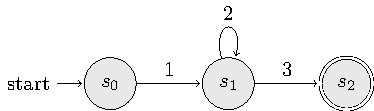
\includegraphics{chapters/cpsystems/ruleset1statemachine.pdf}
    \caption[State machine diagram for the system in \cref{rules:cps:slowmulti}]{State machine diagram for the system in \cref{rules:cps:slowmulti}.  Nodes are labelled with states, and edges with rules transitioning between them}
    \label{fig:cps:slowmulti}
\end{figure}

In particular, it is not possible here to make the second rule work in parallel --- a given functor or atom may only be used in one rule application per system step, and so the first rule application would take exclusive control of both the \(c\) functor and its \(d\) contents, preventing any further rule applications from occurring.  A further wrinkle of this \gls{ruleset} is the fact that it requires an extra temporary functor, \(f\), to store copies of the \(d\) atoms for transfer back into \(c\) at the end because the appropriate termination point for these rules can only be detected when \(c\) has been emptied.

\subsection{A Solution}
To avoid this problem, we revisit and clarify an older and rarely used operation that permits a rule to be applied to the contents of a sub-cell or functor, \emph{without} also seizing control (i.e. locking) of the sub-cell or functor itself.  We term this operation \emph{\gls{ms}}, representing the idea that as-minimal-as-possible modification is made to the containing object while modifying its contents.  We denote \glspl{ms} through the use of curly braces, rather than the usual parentheses for complex terms.  They are still complex terms, but the operation performed on them differs.  Due to this differing operation, every instance of a \gls{ms} on the \gls{lhs} \emph{must} have a matching instance on the \gls{rhs}.

% \cpruleinline{
% \cprule*{s_0}{}{\cponce}{s_1}{\cpfunc{e}{\cpempty}}
% \cprule*{s_1}{\cpfuncms{e}{\cpempty}}{\cpmaxpar}{s_2}{\cpfuncms{e}{B}~|~\cpfunc{c}{d\cpdiscard}~|~\cpfunc{a}{B}}}

% \begin{cprulesetfloat}
%     \begin{cpruleset}
%         \cprule{s_0}{}{\cponce}{s_1}{\cpfunc{e}{\cpempty}}

%         \cprule{s_1}{\cpfuncms{e}{\cpempty}}{\cpmaxpar}{s_2}{\cpfuncms{e}{B}}
%         \cppromoter{\cpfunc{c}{d\cpdiscard}}
%         \cppromoter{\cpfunc{a}{B}}
%     \end{cpruleset}
%     \caption{\label{rules:cps:microsurg}Rules for a destructive multiplication process that requires exactly two steps regardless of the numbers multiplied by using \gls{cps} \glspl{ms}}
% \end{cprulesetfloat}

\begin{cprulesetfloat}
    \begin{cpruleset}
        \cprule{s_0}{}{\cponce}{s_1}{\cpfunc{e}{\cpempty}}

        \cprule{s_1}{\cpfuncms{e}{\,}}{\cpmaxpar}{s_2}{\cpfuncms{e}{B}}
        \cppromoter{\cpfunc{c}{d\cpdiscard}}
        \cppromoter{\cpfunc{a}{B}}
    \end{cpruleset}
    \caption{\label{rules:cps:microsurg}Rules for a destructive multiplication process that requires exactly two steps regardless of the numbers multiplied by using \gls{cps} \glspl{ms}}
\end{cprulesetfloat}

\Cref{rules:cps:microsurg} is an example of three rules using \glspl{ms} that achieve in \emph{two} steps the same destructive multiplication as the \gls{ruleset} listed in \cref{rules:cps:slowmulti}, which requires \(D + 1\) steps.  Crucially, the second rule is still \emph{one} rule application, but the insertion of \(B\) into \(e\) happens once for each possible match on the promoter.  The use of \(c(d\cpdiscard)\) combined with the maximally parallel rule mode means that the rule will take control of and execute once for each \(d\) atom in the multiset labelled by the \(c\) functor.  As such, three lots of \(B\) will be inserted into \(e\) simultaneously while executing this rule under the example described above.

% Furthermore, non-destructive division of \(d\) by \(e\), \(d \div e = f\), could be:
% \cpruleinline{\cprule*{s_1}{\cpfuncms{f}{\cpempty}~\cpfuncms{d}{E}}{\cpmaxpar}{s_1}{f[\cpundig]~\cpfuncms{d}{\cpempty}~|~\cpfunc{e}{E}}}

% Furthermore, destructive division of \(d\) by \(e\), \(d \div e = f\), could be:
% \cpruleinline{\cprule*{s_1}{\cpfuncms{f}{\cpempty}~\cpfuncms{d}{E}}{\cpmaxpar}{s_1}{\cpfuncms{f}{\cpundig}~\cpfuncms{d}{\cpempty}~|~\cpfunc{e}{E}}}

Furthermore, destructive division of \(d\) by \(e\), \(d \div e = f\), could be:
\cpruleinline{\cprule*{s_1}{\cpfuncms{f}{\,}~\cpfuncms{d}{E}}{\cpmaxpar}{s_1}{\cpfuncms{f}{\cpundig}~\cpfuncms{d}{\,}~|~\cpfunc{e}{E}}}

Note that in the case of division, the quotient returned in the \(f\) term will be the \emph{floor} of the precise division result, i.e. the equation could be written as \(\lfloor d \div e \rfloor = f\).  For cases where the dividend is an exact multiple of the divisor, this will be the same as the correct result.  Otherwise, it will be the correct result's whole-number part only.  E.g. referring to the rule immediately above, for \(d(6)~\&~e(3)\), the output will be \(f(2)\), whereas for \(d(5)~\&~e(3)\), the output will be \(f(1)\), with the two left-over unary digits remaining in \(d\).  In other words, \(f\) receives the quotient, and \(d\) keeps the remainder.

\lstset{xleftmargin=.5in, xrightmargin=.5in} 
\begin{lstlisting}
  $\cpfuncms{a}{\cpundig} \; \rightarrow_{\cpmaxpar} \; \cpfuncms{a}{B}~|~\cpfunc{b}{B}$ #\hfill\textsl{single-step multiplication}\enspace#
  $\cpfuncms{a}{C} \; \cpfuncms{b}{\,} \; \rightarrow_{\cpmaxpar} \; \cpfuncms{a}{\,} \; \cpfuncms{b}{\cpundig}~|~\cpfunc{c}{C}$ #\hfill\textsl{single-step floor division}\enspace#
\end{lstlisting}

% To instead achieve ceiling division, first copy the dividend into the receiving term (in the example above, this would be the \(f\) term), and then withdrawing multiples of the divisor from there.  An integer multiple of the divisor will be withdrawn from the receiving term, and the copies of the unary digit added back form the quotient of the division.  The remainder of the division will also be in the receiving term, as it is not removed during the step.  Continuing with the example above, if the contents of the \(d\) term have already been copied into the \(f\) term, then ceiling division can be perfomed via:
\cpruleinline{\cprule*{s_1}{\cpfuncms{f}{E}}{\cpmaxpar}{s_1}{\cpfuncms{f}{\cpundig}~|~\cpfunc{e}{E}}}
%-----------------------------------------------------------------------------------
\section{\label{sec:cps:compoundterms}Indexed notation for compound terms}
%-----------------------------------------------------------------------------------

\emph{Indexed compound terms} are reasonably common in \gls{cps}.  That is, terms tagged with one or more sub-terms used to distinguish different instances of the same functor type.  They are still classic \gls{cps} objects with nested terms, but some of the subterms are used only to distinguish between instances of the encompassing compound term.  This is roughly analogous to tagging a term with its index in a logical vector/array or its key in a typical \fxerror{Need to distinguish this from, or integrate it with, the discussion about data structures above.}{dictionary/associative array data structure.}

For example, in \cref{chap:nmp}, compound \(v\) terms appear in multiple rules.  Ordinarily, these would be represented as nested terms along the lines of
\[ \cpfunc{v}{\cpfunc{v'}{N} \; \cpfunc{v''}{G}\; D} \]
These are used inside \glspl{tlc} to represent sets of tagged data.  They are indexed by neighbour \(N\) and tagged with a `generation count' \(G\) (further explained in \cref{sec:nmp:pespecific}).  Both of these values track metadata about a datum.  Lastly, the datum stored by the encompassing term is given.  In many common programming languages, accessing each datum might be written like \texttt{v[N]}, where \texttt{v} is a dictionary indexed by neighbour.  The \(v\) functors could be written as \[ \cpvv{N}{G}{D} \] for a shorthand that can be expanded back out to a complete form automatically.  The first pair of parentheses selects functors by neighbour, the second records the generation, while the final pair shows the actual contents.  This is \emph{purely} a notational convenience, without impact upon the application of the rules and evolution of the system.  When a concrete instance of a \(v\) compound term is indexed by a ground term (i.e. not a variable) \(k\), e.g. \(\cpvv{k}{\_}{\_}\), it may be referred to as \emph{k-tagged}.

\lstset{xleftmargin=.5in, xrightmargin=.5in} 
\begin{lstlisting}
  $\cpfunc{v}{\cpfunc{v'}{N} \; \cpfunc{v''}{G}\; D}$ #\hfill\textsl{nested functor}\enspace#
  $\cpvv{N}{G}{D}$ #\hfill\textsl{compound term}\enspace#
\end{lstlisting}
% %-----------------------------------------------------------------------------------
% \section{\label{sec-min}Efficient minimum-finding with cP~rules}
% %-----------------------------------------------------------------------------------

% Consider an unstructured multiset $A \subseteq \mathbb{N}$ of size \(n\). 
% It is well known that (1) any sequential algorithm that finds its minimum needs at least \(n\) steps, and 
% (2) any parallel algorithm that finds its minimum needs at least \(\log n\) parallel steps.

% Without loss of generality, consider a \gls{cps} cell, in state \(s_1\), where multiset \(A\) is given via functor \(a\); 
% e.g., multiset \(A = \{ 1, 2, 2, 5 \}\) is represented as \(\cpfunc{a}{1} \, \cpfunc{a}{2} \, \cpfunc{a}{2} \, \cpfunc{a}{5}\).
% The following \glspl{ruleset} implement various versions of a \gls{cps} minimum-finding algorithm.
% All these \glspl{ruleset} transit to state \(s_2\) and construct a term with functor \(b\), containing \(\mathop{min} A\).
% Some of these are destructive processes; if otherwise desired, one could first make a copy of the initial multiset \(A\).

% The following destructive \gls{ruleset} emulates the classical sequential minimum finding algorithm, which takes \(n\) steps:

% \lstset{xleftmargin=.5in, xrightmargin=.5in} 
% \begin{lstlisting}
% $s_1$  $\cpfunc{a}{X}$  $\rightarrow_{1}$  $s_2$  $\cpfunc{b}{X}$ 
% $s_2$  $\cpfunc{a}{XY}$  $\cpfunc{b}{X}$  $\rightarrow_{\cponce}$  $s_2$  $\cpfunc{b}{X}$     #\hfill  $a \geq b  $ \enspace #
% $s_2$  $\cpfunc{a}{X}$  $\cpfunc{b}{X1Y}$  $\rightarrow_{\cponce}$  $s_2$  $\cpfunc{b}{X}$   #\hfill  $a < b  $ \enspace #
% \end{lstlisting}

% The following destructive \gls{ruleset} emulates the classical parallel minimum finding algorithm, which takes \(\log n\) steps.
% As long as there is more than one term \(a\), the \gls{ruleset} loops in state \(s_1\), keeping minima between pairs.
% When only one \(a\) remains (containing the minimum value), the \gls{ruleset} transits to state \(s_2\) and tags the minimum. 

% \lstset{xleftmargin=.5in, xrightmargin=.5in} 
% \begin{lstlisting}
% $s_1$  $\cpfunc{a}{XY}$  $\cpfunc{a}{X}$  $\rightarrow_{\cpmaxpar}$  $s_1$  $\cpfunc{a}{X}$     
% $s_1$  $\cpfunc{a}{X}$  $\cpfunc{a}{X1Y}$  $\rightarrow_{\cpmaxpar}$  $s_1$  $\cpfunc{a}{X}$
% $s_1$  $\cpfunc{a}{X}$  $\rightarrow_{\cponce}$  $s_2$  $\cpfunc{b}{X}$  
% \end{lstlisting}

% However, using the full associative power of \gls{cps}, we can find a non-destructive version with two rules, 
% which works in \emph{just two steps} (regardless of the set cardinality). 
% This is a substantial improvement over existing classical algorithms (both sequential and parallel). 
% It starts by making a full copy of \(a\) as \(b\), in one \(\cpmaxpar\)-parallel step, 
% and then deletes all non-minimal \(b\) values in another \(\cpmaxpar\)-parallel step. 

% \lstset{xleftmargin=.5in, xrightmargin=.5in} 
% \begin{lstlisting}
% $s_1$  $\rightarrow_{\cpmaxpar}$  $s_1'$  $\cpfunc{b}{X}$    $\mid$  $\cpfunc{a}{X}$  
% $s_1'$  $\cpfunc{b}{X1Y}$  $\rightarrow_{\cpmaxpar}$  $s_2$    $\mid$  $\cpfunc{a}{X}$  
% \end{lstlisting}

% Note that if the minimum value appears several times in multiset \(A\), 
% then we will end with the same multiplicity of \(b\)'s, each one containing the same value, \(\mathop{min} A\).
% If required, there are several ways to select only one copy and delete the rest, but we do not deal with this issue further here.

% Moreover, using the full power of cP~inhibitors (as logical negations, with local variables), 
% we can even non-destructively solve the problem in just \emph{one single step},
% with one or two rules.
% This version is implemented by the following \gls{ruleset}:

% \lstset{xleftmargin=.5in, xrightmargin=.5in} 
% \begin{lstlisting}
% $s_1$  $\rightarrow_{\cponce}$  $s_2$  $\cpfunc{b}{}$    $\mid$  $\cpfunc{a}{}$
% $s_1$  $\rightarrow_{\cponce}$  $s_2$  $\cpfunc{b}{1Z}$     $\mid$  $\cpfunc{a}{1Z}$     $\neg$  $(Z=XY)$  $\cpfunc{a}{X}$
% \end{lstlisting}

% If \(A\) contains zero, then there is a term \(\cpfunc{a}{}\), and: (1) the first rule applies, constructing \(\cpfunc{b}{}\); (2) the second rule is not applicable.
% Otherwise, (if there is no zero in \(A\)): (1) the first rule is not applicable; (2) the second rule constructs \(\cpfunc{b}{1Z}\), 
% a value which exists among \(a\)'s, as \(\cpfunc{a}{1Z}\), but there is NO other \(a\) containing a strictly lesser value, such as \(\cpfunc{a}{X}\),
% where \(X\) is a sub-multiset of \(Z\), \(X \subseteq Z\).
% Finally, the newly constructed \(b\) will contain one copy of the minimum value of multiset \(A\).

% If multiset \(A\) does not contain zero values, i.e. \(A \subseteq \mathbb{N}^+\), then the first rule can be safely omitted (as it will never be applicable). 
% A similar \gls{ruleset} can be devised for finding the maximum of a given set of natural numbers.

% %%%%%%%%%%%%%%%%%%%%%%%%%%%%%%%%%%%%%%%%%%%%%%%%%%%%%%%%%%%%%%%%%%%%%%%%%%%%%%%%%%%%%%%%
% %%%%%%%%%%%%%%%%%%%%%%%%%%%%%%%%%%%%%%%%%%%%%%%%%%%%%%%%%%%%%%%%%%%%%%%%%%%%%%%%%%%%%%%%
% %%%%%%%%%%%%%%%%%%%%%%%%%%%%%%%%%%%%%%%%%%%%%%%%%%%%%%%%%%%%%%%%%%%%%%%%%%%%%%%%%%%%%%%%
% %%%%%%%%%%%%%%%%%%%%%%%%%%%%%%%%%%%%%%%%%%%%%%%%%%%%%%%%%%%%%%%%%%%%%%%%%%%%%%%%%%%%%%%%

%-----------------------------------------------------------------------------------
\section{Statistical Operations}\label{sec:cps:stats}
%-----------------------------------------------------------------------------------

This section presents and discusses procedures in \gls{cps} for the following fundamental statistical operations on numerical sets and multisets:
\begin{itemize}
    \item Finding the minimum and maximum elements.
    \item Determining the overall number and counting the frequency of elements.
    \item Computing the sum, mean, and mode over all elements.
    \item Sorting elements.
    \item Selecting the \(n^{\text{th}}\) (and thus median) element.
\end{itemize}

Leveraging the power of \gls{cps} -- logical pattern matching on associative data objects -- \emph{all} of the presented procedures run in constant time O\((1)\) and require small, fixed \glspl{ruleset} for all cases.  For brevity, these rules consider only the case of non-empty (multi)sets of natural numbers greater than zero (\(\mathbb{N}^+\)), and their total order (\(\leq\)).  Extensions to handle zero values and empty sets are not complicated, but would inflate \glspl{ruleset} by a few additional rules without adding significant value (although they would not alter the time complexity).

At the start (``step 0'') of each presented operation, assume an arbitrary non-empty set or multiset of \(s\) objects, which each hold an arbitrary number.  For each example with a set, the starting \(s\) terms assumed present are:  \[S_1 = \cpset{\cpfunc{s}{2}, \cpfunc{s}{3}, \cpfunc{s}{5}, \cpfunc{s}{6}, \cpfunc{s}{7}}\]  Likewise, the assumed multiset is \[S_2 = \cpset{\cpfunc{s}{2}, \cpfunc{s}{2}, \cpfunc{s}{3}, \cpfunc{s}{5}, \cpfunc{s}{5}, \cpfunc{s}{6}, \cpfunc{s}{6}, \cpfunc{s}{6}, \cpfunc{s}{7}}\]  In almost all cases, the operations apply equally to sets and multisets, so the examples assume the presence of \(S_2\) inside the top-level cell.  The exceptions to that are in \cref{sec:cps:sortsets} and \cref{sec:cps:selectsets}, where \(S_1\) is assumed instead, and \cref{sec:cps:sortmultisetid} and \cref{sec:cps:sortmultisetid}, which use \(S_2\) with an additional datum for each element.  The rules provided are all non-destructive with respect to the (multi)set \(S\).  Destructive versions are simple to derive from the non-destructive ones, so are omitted.

In all cases, the rules are written so that the final result is found in one or more \(r\) functor objects, as appropriate.  Examples of the evolution are given in tabular form immediately after the rules for each operation.  Each table lists \emph{only} the newly created, modified, and deleted objects in the top-level cell at the end of that step.  Modified objects are presented with their outermost functor in boldface, e.g., \(\cpfunc{r}{0}\) to \(\mathbf{\cpfunc{r}{4}}\).  Deleted objects are struck out, e.g., \(\cpfunc{r'}{2}\) to \sout{\(\cpfunc{r'}{2}\)}.

%%%%%%%%%%%%%%%%%%

%-------------------------------------------------------
\subsection{\label{sec:cps:minmax}Minimum and Maximum}
%-------------------------------------------------------

%-----------------------------------------------------------------------------------
% \section{\label{sec-min}Efficient minimum-finding with cP~rules}
%-----------------------------------------------------------------------------------

Consider an unstructured multiset $A \subseteq \mathbb{N}$ of size \(n\). 
It is well known that (1) any sequential algorithm that finds its minimum needs at least \(n\) steps, and 
(2) any parallel algorithm that finds its minimum needs at least \(\log n\) parallel steps.

Without loss of generality, consider a \gls{cps} cell, in state \(s_1\), where multiset \(A\) is given via functor \(a\); 
e.g., multiset \(A = \{ 1, 2, 2, 5 \}\) is represented as \(\cpfunc{a}{1} \, \cpfunc{a}{2} \, \cpfunc{a}{2} \, \cpfunc{a}{5}\).
The following \glspl{ruleset} implement various versions of a \gls{cps} minimum-finding algorithm.
All these \glspl{ruleset} transit to state \(s_2\) and construct a term with functor \(b\), containing \(\mathop{min} A\).
Some of these are destructive processes; if otherwise desired, one could first make a copy of the initial multiset \(A\).

The following destructive \gls{ruleset} emulates the classical sequential minimum finding algorithm, which takes \(n\) steps:

\lstset{xleftmargin=.5in, xrightmargin=.5in} 
\begin{lstlisting}
$s_1$  $\cpfunc{a}{X}$  $\rightarrow_{1}$  $s_2$  $\cpfunc{b}{X}$ 
$s_2$  $\cpfunc{a}{XY}$  $\cpfunc{b}{X}$  $\rightarrow_{\cponce}$  $s_2$  $\cpfunc{b}{X}$     #\hfill  $a \geq b  $ \enspace #
$s_2$  $\cpfunc{a}{X}$  $\cpfunc{b}{X1Y}$  $\rightarrow_{\cponce}$  $s_2$  $\cpfunc{b}{X}$   #\hfill  $a < b  $ \enspace #
\end{lstlisting}

The following destructive \gls{ruleset} emulates the classical parallel minimum finding algorithm, which takes \(\log n\) steps.
As long as there is more than one term \(a\), the \gls{ruleset} loops in state \(s_1\), keeping minima between pairs.
When only one \(a\) remains (containing the minimum value), the \gls{ruleset} transits to state \(s_2\) and tags the minimum. 

\lstset{xleftmargin=.5in, xrightmargin=.5in} 
\begin{lstlisting}
$s_1$  $\cpfunc{a}{XY}$  $\cpfunc{a}{X}$  $\rightarrow_{\cpmaxpar}$  $s_1$  $\cpfunc{a}{X}$     
$s_1$  $\cpfunc{a}{X}$  $\cpfunc{a}{X1Y}$  $\rightarrow_{\cpmaxpar}$  $s_1$  $\cpfunc{a}{X}$
$s_1$  $\cpfunc{a}{X}$  $\rightarrow_{\cponce}$  $s_2$  $\cpfunc{b}{X}$  
\end{lstlisting}

However, using the full associative power of \gls{cps}, we can find a non-destructive version with two rules, 
which works in \emph{just two steps} (regardless of the set cardinality). 
This is a substantial improvement over existing classical algorithms (both sequential and parallel). 
It starts by making a full copy of \(a\) as \(b\), in one \(\cpmaxpar\)-parallel step, 
and then deletes all non-minimal \(b\) values in another \(\cpmaxpar\)-parallel step. 

\lstset{xleftmargin=.5in, xrightmargin=.5in} 
\begin{lstlisting}
$s_1$  $\rightarrow_{\cpmaxpar}$  $s_1'$  $\cpfunc{b}{X}$    $\mid$  $\cpfunc{a}{X}$  
$s_1'$  $\cpfunc{b}{X1Y}$  $\rightarrow_{\cpmaxpar}$  $s_2$    $\mid$  $\cpfunc{a}{X}$  
\end{lstlisting}

Note that if the minimum value appears several times in multiset \(A\), 
then we will end with the same multiplicity of \(b\)'s, each one containing the same value, \(\mathop{min} A\).
If required, there are several ways to select only one copy and delete the rest, but we do not deal with this issue further here.

Moreover, using the full power of cP~inhibitors (as logical negations, with local variables), 
we can even non-destructively solve the problem in just \emph{one single step},
with one or two rules.
This version is implemented by the following \gls{ruleset}:

\lstset{xleftmargin=.5in, xrightmargin=.5in} 
\begin{lstlisting}
$s_1$  $\rightarrow_{\cponce}$  $s_2$  $\cpfunc{b}{}$    $\mid$  $\cpfunc{a}{}$
$s_1$  $\rightarrow_{\cponce}$  $s_2$  $\cpfunc{b}{1Z}$     $\mid$  $\cpfunc{a}{1Z}$     $\neg$  $(Z=XY)$  $\cpfunc{a}{X}$
\end{lstlisting}

If \(A\) contains zero, then there is a term \(\cpfunc{a}{}\), and: (1) the first rule applies, constructing \(\cpfunc{b}{}\); (2) the second rule is not applicable.
Otherwise, (if there is no zero in \(A\)): (1) the first rule is not applicable; (2) the second rule constructs \(\cpfunc{b}{1Z}\), 
a value which exists among \(a\)'s, as \(\cpfunc{a}{1Z}\), but there is NO other \(a\) containing a strictly lesser value, such as \(\cpfunc{a}{X}\),
where \(X\) is a sub-multiset of \(Z\), \(X \subseteq Z\).
Finally, the newly constructed \(b\) will contain one copy of the minimum value of multiset \(A\).

If multiset \(A\) does not contain zero values, i.e. \(A \subseteq \mathbb{N}^+\), then the first rule can be safely omitted (as it will never be applicable). 
A similar \gls{ruleset} can be devised for finding the maximum of a given set of natural numbers.

The rules of this \namecref{sec:cps:minmax} apply equally to sets and multisets.  The \glspl{ruleset} of this  \namecref{sec:cps:minmax} are notable as being two of only three in this work to use inhibitors, while the third, \cref{rules:cps:mode}, essentially performs maximum selection as part of its process.  An alternative approach forgoing inhibitors is described in \cite{Nicolescu2018} if needed.

%-----------------------------------------
\subsubsection{Minimum --- O\((1)\)}\label{sec:cps:min}
%-----------------------------------------

\begin{proposition}\label{prop:cps:min}
Finding the minimum takes one step.
\end{proposition}

\begin{proof}
Consider \cref{rules:cps:min} and the example in \cref{tab:cps:min}.  The rule to find the minimum selects an \(s\) term's value, such that there is no other \(s\) with a strictly lower value.
\end{proof}

\begin{cprulesetfloat}
\begin{cpruleset}
\cprule*{s_1}{}{\cponce}{s_2}{\cpfunc{r}{R\cpundig T}}
\cppromoter{\cpfunc{s}{R\cpundig T}}
\cpinhibitor{\cpfunc{s}{R}}
\end{cpruleset}
\caption{\label{rules:cps:min}\Gls{ruleset} to find the minimum element in a (multi)set}
\end{cprulesetfloat}

\begin{table}
\centering
\begin{tabular}{|r|l|}
    \hline
    \textbf{Step} & \textbf{New, Modified or Deleted Objects} \\ \hline
    1 & \(\cpfunc{r}{2}\)\\ \hline
\end{tabular}
\caption[Example evolution of \cref{rules:cps:min}]{\label{tab:cps:min}Example evolution of \cref{rules:cps:min} starting on multiset \(S_2\)}
\end{table}

%-----------------------------------------
\subsubsection{\label{sec:cps:max}Maximum --- O\((1)\)}
%-----------------------------------------

\begin{proposition}\label{prop:cps:max}
Finding the maximum takes one step.
\end{proposition}

\begin{proof}
Consider \cref{rules:cps:max} and the example in \cref{tab:cps:max}.  The rule to find the maximum selects an \(s\) term's value, such that there is no other \(s\) with a strictly higher value.
\end{proof}

\begin{cprulesetfloat}
\begin{cpruleset}

\cprule*{s_1}{}{\cponce}{s_2}{\cpfunc{r}{R}}
\cppromoter{\cpfunc{s}{R}}
\cpinhibitor{\cpfunc{s}{R\cpundig \_}}

\end{cpruleset}
\caption{\label{rules:cps:max}\Gls{ruleset} to find the maximum element in a (multi)set}
\end{cprulesetfloat}

\begin{table} \centering
\begin{tabular}{|r|l|}
    \hline
    \textbf{Step} & \textbf{New, Modified or Deleted Objects} \\ \hline
    1 & \(\cpfunc{r}{7}\)\\ \hline
\end{tabular} 
\caption[Example evolution of \cref{rules:cps:max}]{\label{tab:cps:max}Example evolution of \cref{rules:cps:max} starting on multiset \(S_2\)}
\end{table}

%%%%%%%%%%%%%%%%%%

%-------------------------------------------------------
\subsection{Counting}\label{sec:cps:counting}
%-------------------------------------------------------

%-----------------------------------------
\subsubsection{Counting Elements --- O\((1)\)}\label{sec:cps:countelems}
%-----------------------------------------

\begin{proposition}\label{prop:cps:countelems}
Determining the magnitude of a (multi)set takes two steps.
\end{proposition}

\begin{proof}
Consider \cref{rules:cps:countelems} and the example in \cref{tab:cps:countelems}.  The first rule creates an empty term to store the result, and then the second rule tallies the elements present.
\end{proof}

\begin{cprulesetfloat} \begin{cpruleset}

\cprule{s_1}{}{\cponce}{s_2}{\cpfunc{r}{\cpempty}}

\cprule{s_2}{\cpfuncms{r}{\,}}{\cpmaxpar}{s_3}{\cpfuncms{r}{\cpundig}}
\cppromoter{\cpfunc{s}{\_}}

\end{cpruleset}
\caption{\label{rules:cps:countelems}\Gls{ruleset} to find the magnitude of a (multi)set}
\end{cprulesetfloat}

\begin{table} \centering
   \begin{tabular}{|r|l|}
    \hline
    \textbf{Step} & \textbf{New, Modified or Deleted Objects} \\ \hline
    1 & \(\cpfunc{r}{0}\)\\ \hline
    
    2 & \(\mathbf{\cpfunc{r}{9}}\)\\ \hline
\end{tabular}
\caption[Example evolution of \cref{rules:cps:countelems}]{\label{tab:cps:countelems}Example evolution of \cref{rules:cps:countelems} starting on multiset \(S_2\)}
\end{table}

%-----------------------------------------
\subsubsection{Counting Frequency of Elements --- O\((1)\)}\label{sec:cps:countfreq}
%-----------------------------------------

\begin{proposition}\label{prop:cps:countfreq}
Counting the occurrence -- essentially creating a histogram -- of the values in a multiset takes three steps.
\end{proposition}

\begin{proof}
Consider \cref{rules:cps:countfreq} and the example in \cref{tab:cps:countfreq}.  The first rule creates a tally \(r\) term for every \(s\) term, while the second rule eliminates any ensuing duplicates, leaving only one \(r\) per unique value stored in any \(s\).  Lastly, rule 3 performs a similar operation to \cref{sec:cps:countelems}, incrementing each \(r\) term's tally by one for each \(s\) term containing the corresponding value.
\end{proof}

% \cpresetrulenumber
\begin{cprulesetfloat}
\begin{cpruleset}
\cprule{s_1}{}{\cpmaxpar}{s_2}{\cpfuncn{r}{R}{\cpempty}}
\cppromoter{\cpfunc{s}{R}}

\cprule{s_2}{\cpfuncn{r}{R}{\_}}{\cpmaxpar}{s_3}{}
\cppromoter{\cpfuncn{r}{R}{\_}}

\cprule{s_3}{\cpfuncnms{r}{R}{\,}}{\cpmaxpar}{s_4}{\cpfuncnms{r}{R}{\cpundig}}
\cppromoter{\cpfunc{s}{R}}
\end{cpruleset}
\caption{\label{rules:cps:countfreq}\Gls{ruleset} to count the occurrence frequency of elements in a multiset}
\end{cprulesetfloat}

\begin{table} \centering
   \begin{tabular}{|r|l|}
    \hline
    \textbf{Step} & \textbf{New, Modified or Deleted Objects} \\ \hline
    1 & \(\cpfuncn{r}{2}{0}\), \(\cpfuncn{r}{2}{0}\), \(\cpfuncn{r}{3}{0}\), \(\cpfuncn{r}{5}{0}\), \(\cpfuncn{r}{5}{0}\), \(\cpfuncn{r}{6}{0}\), \(\cpfuncn{r}{6}{0}\), \(\cpfuncn{r}{6}{0}\), \(\cpfuncn{r}{7}{0}\)\\ \hline
    
    % 2 & \sout{\(\cpfuncn{r}{2}{0}\)}, \sout{\(\cpfuncn{r}{5}{0}\)}, \sout{\(\cpfuncn{r}{6}{0}\)}, \sout{\(\cpfuncn{r}{6}{0}\)}\\ \hline
    
    2 & \(\cpfuncn{r}{2}{0}\), \sout{\(\cpfuncn{r}{2}{0}\)}, \(\cpfuncn{r}{3}{0}\), \(\cpfuncn{r}{5}{0}\), \sout{\(\cpfuncn{r}{5}{0}\)}, \(\cpfuncn{r}{6}{0}\), \sout{\(\cpfuncn{r}{6}{0}\)}, \sout{\(\cpfuncn{r}{6}{0}\)}, \(\cpfuncn{r}{7}{0}\)\\ \hline
    
    3 & \(\mathbf{\cpfuncn{r}{2}{2}}\), \(\mathbf{\cpfuncn{r}{3}{1}}\), \(\mathbf{\cpfuncn{r}{5}{2}}\), \(\mathbf{\cpfuncn{r}{6}{3}}\), \(\mathbf{\cpfuncn{r}{7}{1}}\)\\ \hline
\end{tabular}
\caption[Example evolution of \cref{rules:cps:countfreq}]{\label{tab:cps:countfreq}Example evolution of \cref{rules:cps:countfreq} starting on multiset \(S_2\)}
\end{table}

\Cref{rules:cps:countfreq} works equally well for sets, but the frequency of each element present will be one due to the nature of a set.

%-------------------------------------------------------
\subsection{Sum, Mean and Mode}\label{sec:cps:sumeanmode}
%-------------------------------------------------------

%-----------------------------------------
\subsubsection{Sum --- O\((1)\)}\label{sec:cps:sum}
%-----------------------------------------

\begin{proposition}\label{prop:cps:sum}
Computing the sum of the elements in a (multi)set requires two steps.
\end{proposition}

\begin{proof}
Consider \cref{rules:cps:sum} and the example in \cref{tab:cps:sum}.  These rules act very similarly to \cref{sec:cps:countelems}, but add the total stored value in every \(s\) term to the \(r\) term, rather than simply one \(\cpundig\) per \(s\) term.
\end{proof}

% \cpresetrulenumber
\begin{cprulesetfloat} \begin{cpruleset}
\cprule{s_1}{}{\cponce}{s_2}{\cpfunc{r}{\cpempty}}
\cprule{s_2}{\cpfuncms{r}{\,}}{\cpmaxpar}{s_3}{\cpfuncms{r}{R}}
\cppromoter{\cpfunc{s}{R}}
\end{cpruleset}
\caption{\label{rules:cps:sum}\Gls{ruleset} to find the sum of numeric elements in a (multi)set}
\end{cprulesetfloat}

\begin{table} \centering
   \begin{tabular}{|r|l|}
    \hline
    \textbf{Step} & \textbf{New, Modified or Deleted Objects} \\ \hline
    1 & \(\cpfunc{r}{0}\)\\ \hline
    2 & \(\cpfunc{r}{42}\)\\ \hline

\end{tabular}
\caption[Example evolution of \cref{rules:cps:sum}]{\label{tab:cps:sum}Example evolution of \cref{rules:cps:sum} starting on multiset \(S_2\)}
\end{table}

%-----------------------------------------
\subsubsection{Mean --- O\((1)\)}\label{sec:cps:mean}
%-----------------------------------------

\begin{proposition}\label{prop:cps:mean}
Finding the (whole number) mean of a (multi)set requires four steps.
\end{proposition}

\begin{proof}
Consider \cref{rules:cps:mean} and the example in \cref{tab:cps:mean}.  Computing the mean is mostly a combination of two previous operations:  Sum the elements (\cref{sec:cps:sum}), and divide by the count of elements (\cref{sec:cps:countelems}).  The summing and counting may be performed simultaneously in two steps, with two extra steps for the division.
\end{proof}

% \cpresetrulenumber
\begin{cprulesetfloat}
\begin{cpruleset}
\cprule{s_1}{}{\cponce}{s_2}{\cpfunc{c}{\cpempty} \; \cpfunc{r}{\cpempty} \; \cpfunc{r'}{\cpempty}}

\cprule{s_2}{\cpfuncms{c}{\,}}{\cpmaxpar}{s_3}{\cpfuncms{c}{\cpundig}}
\cppromoter{\cpfunc{s}{\_}}

\cprule{s_2}{\cpfuncms{r}{\,} \; \cpfuncms{r'}{\,}}{\cpmaxpar}{s_3}{\cpfuncms{r}{R} \; \cpfuncms{r'}{R}}
\cppromoter{\cpfunc{s}{R}}

\cprule{s_3}{\cpfuncms{r}{C} \; \cpfuncms{r'}{C}}{\cpmaxpar}{s_4}{\cpfuncms{r}{\cpundig} \; \cpfuncms{r'}{\,}}
\cppromoter{\cpfunc{c}{C}}

\cprule{s_4}{\cpfunc{r}{QR} \; \cpfunc{r'}{R}}{\cponce}{s_5}{\cpfunc{r}{Q}}
\end{cpruleset}
\caption{\label{rules:cps:mean}\Gls{ruleset} to find the mean of elements in a (multi)set}
\end{cprulesetfloat}

\begin{table} \centering
  \begin{tabular}{|r|l|}
    \hline
    \textbf{Step} & \textbf{New, Modified or Deleted Objects} \\ \hline
    1 & \(\cpfunc{c}{0}\), \(\cpfunc{r}{0}\), \(\cpfunc{r'}{0}\)\\ \hline
    2 & \(\mathbf{\cpfunc{c}{9}}\), \(\mathbf{\cpfunc{r}{42}}\), \(\mathbf{\cpfunc{r'}{42}}\)\\ \hline
    3 & \(\mathbf{\cpfunc{r}{11}}\), \(\mathbf{\cpfunc{r'}{6}}\)\\ \hline
    4 & \(\mathbf{\cpfunc{r}{5}}\), \sout{\(\cpfunc{r'}{6}\)}\\ \hline

\end{tabular}
\caption[Example evolution of \cref{rules:cps:mean}]{\label{tab:cps:mean}Example evolution of \cref{rules:cps:mean} starting on multiset \(S_2\)}
\end{table}

Rules 4 and 5 perform ceiling integer division.  Rule 4 removes \(C\) copies of the unary digit from \(r\) and adds one copy back to it.  This is repeated as many times as possible, given the number of digits available.  What is left in \(r\) at the end of the step is, in effect, the quotient plus the remainder.  In this example, with a count of nine and a sum of forty-two, the removal can be applied four times, for a total of thirty-six unary digits removed.  Five more are added at the end of the step, meaning a total of eleven remains.  This is not the correct result of ceiling integer division but is the correct quotient (5) plus the remainder (6).  Thus, another copy of the total is kept and divided, without the quotient added back in.  This leaves rule 5 to compute the correct final result by deducting the remainder from the combined quotient and remainder.

%-----------------------------------------
\subsubsection{Mode --- O\((1)\)}  \label{sec:cps:mode}
%-----------------------------------------

\begin{proposition}\label{prop:cps:mode}
Finding the mode of the elements in a multiset requires four steps.
\end{proposition}

\begin{proof}
Consider \cref{rules:cps:mode} and the example in \cref{tab:cps:mode}.  As with the mean, this process combines other operations:  Counting the frequency of elements (\cref{sec:cps:countfreq}) takes three steps, then selecting the maximum (\cref{sec:cps:max}) uses one extra step.  Unlike in \cref{sec:cps:mean}, the aforementioned \glspl{ruleset} cannot be used concurrently to reduce the number of steps required because the maximum-finding rule must only fire once the frequency counting process has concluded.
\end{proof}

% \cpresetrulenumber
\begin{cprulesetfloat} \begin{cpruleset}
\cprule{s_1}{}{\cpmaxpar}{s_2}{\cpfuncn{c}{C}{\cpempty}}
\cppromoter{\cpfunc{s}{C}}

\cprule{s_2}{\cpfuncn{c}{C}{\_}}{\cpmaxpar}{s_3}{}
\cppromoter{\cpfuncn{c}{C}{\_}}

\cprule{s_3}{\cpfuncnms{c}{C}{\,}}{\cpmaxpar}{s_4}{\cpfuncnms{c}{C}{\cpundig}}
\cppromoter{\cpfunc{s}{C}}

\cprule{s_4}{}{\cponce}{s_5}{\cpfunc{r}{C}}
\cppromoter{\cpfuncn{c}{C}{R}}
\cpinhibitor{\cpfuncn{c}{\_}{R\cpundig \_}}

\end{cpruleset}
\caption{\label{rules:cps:mode}\Gls{ruleset} to find the mode of the elements in a multiset}
\end{cprulesetfloat}

% \begin{table} \centering
%   \begin{tabular}{|r|l|}
%     \hline
%     \textbf{Step} & \textbf{New, Modified or Deleted Objects} \\ \hline
%     1 & \(\cpfuncn{c}{2}{0}\), \(\cpfuncn{c}{2}{0}\), \(\cpfuncn{c}{3}{0}\), \(\cpfuncn{c}{5}{0}\), \(\cpfuncn{c}{5}{0}\), \(\cpfuncn{c}{6}{0}\), \(\cpfuncn{c}{6}{0}\), \(\cpfuncn{c}{6}{0}\),\\& \(\cpfuncn{c}{7}{0}\)\\ \hline
    
%     2 & \sout{\(\cpfuncn{c}{2}{0}\)}, \sout{\(\cpfuncn{c}{5}{0}\)}, \sout{\(\cpfuncn{c}{6}{0}\)}, \sout{\(\cpfuncn{c}{6}{0}\)}\\ \hline
    
%     3 & \(\mathbf{\cpfuncn{c}{2}{2}}\), \(\mathbf{\cpfuncn{c}{3}{3}}\), \(\mathbf{\cpfuncn{c}{5}{2}}\), \(\mathbf{\cpfuncn{c}{6}{3}}\), \(\mathbf{\cpfuncn{c}{7}{1}}\)\\ \hline
    
%     4 & \(\cpfunc{r}{5}\)\\ \hline
% \end{tabular}
% \caption[Example evolution of \cref{rules:cps:mode}]{\label{tab:cps:mode}Example evolution of \cref{rules:cps:mode} starting on multiset \(S_2\)}
% \end{table}

\begin{table} \centering
   \begin{tabular}{|r|l|}
    \hline
    \textbf{Step} & \textbf{New, Modified or Deleted Objects} \\ \hline
    1 & \(\cpfuncn{c}{2}{0}\), \(\cpfuncn{c}{2}{0}\), \(\cpfuncn{c}{3}{0}\), \(\cpfuncn{c}{5}{0}\), \(\cpfuncn{c}{5}{0}\), \(\cpfuncn{c}{6}{0}\), \(\cpfuncn{c}{6}{0}\), \(\cpfuncn{c}{6}{0}\), \(\cpfuncn{c}{7}{0}\)\\ \hline
    
    2 & \(\cpfuncn{c}{2}{0}\), \sout{\(\cpfuncn{c}{2}{0}\)}, \(\cpfuncn{c}{3}{0}\), \(\cpfuncn{c}{5}{0}\), \sout{\(\cpfuncn{c}{5}{0}\)}, \(\cpfuncn{c}{6}{0}\), \sout{\(\cpfuncn{c}{6}{0}\)}, \sout{\(\cpfuncn{c}{6}{0}\)}, \(\cpfuncn{c}{7}{0}\)\\ \hline
    
    3 & \(\mathbf{\cpfuncn{c}{2}{2}}\), \(\mathbf{\cpfuncn{c}{3}{3}}\), \(\mathbf{\cpfuncn{c}{5}{2}}\), \(\mathbf{\cpfuncn{c}{6}{3}}\), \(\mathbf{\cpfuncn{c}{7}{1}}\)\\ \hline
    
    4 & \(\cpfuncn{c}{2}{2}\), \(\cpfuncn{c}{3}{3}\), \(\cpfuncn{c}{5}{2}\), \(\cpfuncn{c}{6}{3}\), \(\cpfuncn{c}{7}{1}\), \(\cpfunc{r}{5}\)\\ \hline
    
\end{tabular}
\caption[Example evolution of \cref{rules:cps:mode}]{\label{tab:cps:mode}Example evolution of \cref{rules:cps:mode} starting on multiset \(S_2\)}
\end{table}

%-------------------------------------------------------
\subsection{Sorting}\label{sec:cps:sorting}
%-------------------------------------------------------

In the current context, sorting is defined as appropriately associating each datum/element in a (multi)set with an ordered index in the range \([1,n]\), where \(n\) is equal to the magnitude (count of elements) of the (multi)set.\footnote{This can easily be switched to \([0,n)\) if desired.}  At the end of the process, the values in the (multi)set shall be sorted in typical ascending numerical order by associating indices with them.

For example, in the context of \(S_2\), this will be 
\begin{align*}
    \text{Element:}& &2 &&2 &&3 &&5 &&5 &&6 &&6 &&6 &&7\\
    \text{Index:}&   &1 &&2 &&3 &&4 &&5 &&6 &&7 &&8 &&9\\
\end{align*}

\Cref{sec:cps:sortsets} \& \cref{sec:cps:sortmultisetid} associate each element with the index individually, while \cref{sec:cps:sortmultisetrange} groups identical multiset elements into ranges spanning the correct indices.

%-----------------------------------------
\subsubsection{Sorting Sets --- O\((1)\)}  \label{sec:cps:sortsets}
%-----------------------------------------

\begin{proposition}\label{prop:cps:sortsets}
Sorting sets requires two steps.
\end{proposition}

\begin{proof}
Consider \cref{rules:cps:sortsets} and the example in \cref{tab:cps:sortsets}.  The rules for sorting a set work similarly to those for counting the frequency of elements (\cref{sec:cps:countfreq}).  Instead of counting the occurrence of a particular value, however, these rules count the occurrence of values strictly less than the current value.  In each instance, this number plus one is equal to the value's correct index in the total ordering, thus sorting the values.
\end{proof}

% \cpresetrulenumber
\begin{cprulesetfloat} \begin{cpruleset}
\cprule{s_1}{}{\cpmaxpar}{s_2}{\cpfuncn{r}{R}{\cpundig}}
\cppromoter{\cpfunc{s}{R}}

\cprule{s_2}{\cpfuncnms{r}{Y}{\,}}{\cpmaxpar}{s_3}{\cpfuncnms{r}{Y}{\cpundig}}
\cppromoter{\cpfunc{s}{X}}
\cppromoter{X \subsetneq Y}
\end{cpruleset}
\caption{\label{rules:cps:sortsets}\Gls{ruleset} to sort the elements in a set}
\end{cprulesetfloat}

\begin{table} \centering
   \begin{tabular}{|r|l|}
    \hline
    \textbf{Step} & \textbf{New, Modified or Deleted Objects} \\ \hline
    1 & \(\cpfuncn{r}{2}{1}\), \(\cpfuncn{r}{3}{1}\), \(\cpfuncn{r}{5}{1}\), \(\cpfuncn{r}{6}{1}\), \(\cpfuncn{r}{7}{1}\)\\ \hline
    2 & \(\cpfuncn{r}{2}{1}\), \(\mathbf{\cpfuncn{r}{3}{2}}\), \(\mathbf{\cpfuncn{r}{5}{3}}\), \(\mathbf{\cpfuncn{r}{6}{4}}\), \(\mathbf{\cpfuncn{r}{7}{5}}\)\\ \hline

\end{tabular}
\caption[Example evolution of \cref{rules:cps:sortsets}]{\label{tab:cps:sortsets}Example evolution of \cref{rules:cps:sortsets} starting on set \(S_1\)}
\end{table}

%-----------------------------------------
\subsubsection{Sorting Multisets into Ranges --- O\((1)\)}\label{sec:cps:sortmultisetrange}
%-----------------------------------------

\begin{proposition}\label{prop:cps:sortmultisetrange}
Sorting a multiset into ordered, indexed ranges requires four steps.
\end{proposition}

\begin{proof}
Consider \cref{rules:cps:sortmultisetrange} and the example in \cref{tab:cps:sortmultisetrange}.  In these rules, the last two numbers for each ending \(t\) object give a range of indices -- with inclusive lower bounds and exclusive upper bounds -- in which the \(s\) numbers of the multiset may be found once ordered.  It requires four steps and relies on the fact that elements of the same value in a multiset are indistinguishable, and thus can be ordered among themselves arbitrarily.

% Consider \cref{rules:cps:sortmultisetrange} and the example in \crefrange{objs:cps:sortmultisetrange:0}{objs:cps:sortmultisetrange:4}.  In these rules, the last two numbers for each ending \(t\) object give a range of indices -- with inclusive lower bounds and exclusive upper bounds -- in which the \(s\) numbers of the multiset may be found once ordered.  It requires four steps and relies on the fact that elements of the same value in a multiset are indistinguishable, and thus can be ordered among themselves arbitrarily.
\end{proof}

% \cpresetrulenumber
\begin{cprulesetfloat} \begin{cpruleset}
\cprule{s_1}{}{\cpmaxpar}{s_2}{\cpfuncnn{r}{R}{\cpundig}{\cpundig}}
\cppromoter{\cpfunc{s}{R}}

\cprule{s_2}{\cpfuncnn{r}{R}{\_}{\_}}{\cpmaxpar}{s_3}{}
\cppromoter{\cpfuncnn{r}{R}{\_}{\_}}

% \cprule{s_3}{\cpfunc{r}{R}}{\cpmaxpar}{s_4}{\cpfuncnn{r}{R}{\cpundig}{\cpundig}}

\cprule{s_3}{\cpfunc{r}{Y}\{\,\}\{\,\}}{\cpmaxpar}{s_4}{\cpfunc{r}{Y}\{\cpundig\}\{\cpundig\}}
\cppromoter{\cpfunc{s}{X}}
\cppromoter{X \subsetneq Y}

\cprule{s_4}{\cpfuncnnms{r}{R}{X}{\,}}{\cpmaxpar}{s_5}{\cpfuncnnms{r}{R}{X}{\cpundig}}
\cppromoter{\cpfunc{s}{R}}

\end{cpruleset}
\caption{\label{rules:cps:sortmultisetrange}\Gls{ruleset} to sort the elements of a multiset into indexed ranges}
\end{cprulesetfloat}

\begin{table} \centering
  \begin{tabular}{|r|l|}
    \hline
    \textbf{Step} & \textbf{New, Modified or Deleted Objects} \\ \hline
    1 & \(\cpfuncnn{r}{2}{1}{1}\), \(\cpfuncnn{r}{2}{1}{1}\), \(\cpfuncnn{r}{3}{1}{1}\), \(\cpfuncnn{r}{5}{1}{1}\), \(\cpfuncnn{r}{5}{1}{1}\), \(\cpfuncnn{r}{6}{1}{1}\),\\& \(\cpfuncnn{r}{6}{1}{1}\), \(\cpfuncnn{r}{6}{1}{1}\), \(\cpfuncnn{r}{7}{1}{1}\)\\ \hline
    
    2 & \(\cpfuncnn{r}{2}{1}{1}\), \sout{\(\cpfuncnn{r}{2}{1}{1}\)}, \(\cpfuncnn{r}{3}{1}{1}\), \(\cpfuncnn{r}{5}{1}{1}\), \sout{\(\cpfuncnn{r}{5}{1}{1}\)}, \(\cpfuncnn{r}{6}{1}{1}\),\\& \sout{\(\cpfuncnn{r}{6}{1}{1}\)}, \sout{\(\cpfuncnn{r}{6}{1}{1}\)}, \(\cpfuncnn{r}{7}{1}{1}\)\\ \hline
    
    % 2 & \sout{\(\cpfuncnn{r}{2}{1}{1}\)}, \sout{\(\cpfuncnn{r}{5}{1}{1}\)}, \sout{\(\cpfuncnn{r}{6}{1}{1}\)}, \sout{\(\cpfuncnn{r}{6}{1}{1}\)}\\ \hline
    
    3 & \(\cpfuncnn{r}{2}{1}{1}\), \(\mathbf{\cpfuncnn{r}{3}{3}{3}}\), \(\mathbf{\cpfuncnn{r}{5}{4}{4}}\), \(\mathbf{\cpfuncnn{r}{6}{6}{6}}\), \(\mathbf{\cpfuncnn{r}{7}{9}{9}}\)\\ \hline
    
    4 & \(\mathbf{\cpfuncnn{r}{2}{1}{3}}\), \(\mathbf{\cpfuncnn{r}{3}{3}{4}}\), \(\mathbf{\cpfuncnn{r}{5}{4}{6}}\), \(\mathbf{\cpfuncnn{r}{6}{6}{9}}\), \(\mathbf{\cpfuncnn{r}{7}{9}{10}}\)\\ \hline
\end{tabular} 
\caption[Example evolution of \cref{rules:cps:sortmultisetrange}]{\label{tab:cps:sortmultisetrange}Example evolution of \cref{rules:cps:sortmultisetrange} starting on multiset \(S_2\)}
\end{table}

% \begin{cpobjectsfloat}
% \begin{cpobjects}
% \cpobjectsline{\cpfunc{s}{2} \, \cpfunc{s}{2} \, \cpfunc{s}{3} \, \cpfunc{s}{5} \, \cpfunc{s}{5} \, \cpfunc{s}{6} \, \cpfunc{s}{6} \, \cpfunc{s}{6} \, \cpfunc{s}{7}}
% \end{cpobjects}
% \caption{\label{objs:cps:sortmultisetrange:0} Objects inside a \gls{tlc} initially containing set \(S_2\), after step 0 of \cref{rules:cps:sortmultisetrange}.}
% \end{cpobjectsfloat}

% \begin{cpobjectsfloat}
% \begin{cpobjects}
% \cpobjectsline{\cpfunc{s}{2} \, \cpfunc{s}{2} \, \cpfunc{s}{3} \, \cpfunc{s}{5} \, \cpfunc{s}{5} \, \cpfunc{s}{6} \, \cpfunc{s}{6} \, \cpfunc{s}{6} \, \cpfunc{s}{7} \quad \cpfuncnn{r}{2}{1}{1} \; \cpfuncnn{r}{2}{1}{1}}
% \cpobjectsline{\cpfuncnn{r}{3}{1}{1} \; \cpfuncnn{r}{5}{1}{1} \; \cpfuncnn{r}{5}{1}{1} \; \cpfuncnn{r}{6}{1}{1} \; \cpfuncnn{r}{6}{1}{1} \; \cpfuncnn{r}{6}{1}{1} \; \cpfuncnn{r}{7}{1}{1}}
% \end{cpobjects}
% \caption{\label{objs:cps:sortmultisetrange:1} Objects inside a \gls{tlc} initially containing set \(S_2\), after step 1 of \cref{rules:cps:sortmultisetrange}.}
% \end{cpobjectsfloat}

% \begin{cpobjectsfloat}
% \begin{cpobjects}
% \cpobjectsline{\cpfunc{s}{2} \, \cpfunc{s}{2} \, \cpfunc{s}{3} \, \cpfunc{s}{5} \, \cpfunc{s}{5} \, \cpfunc{s}{6} \, \cpfunc{s}{6} \, \cpfunc{s}{6} \, \cpfunc{s}{7} \quad \cpfuncnn{r}{2}{1}{1} \; \cpfuncnn{r}{3}{1}{1}}
% \cpobjectsline{\cpfuncnn{r}{5}{1}{1} \; \cpfuncnn{r}{6}{1}{1} \; \cpfuncnn{r}{7}{1}{1}}
% \end{cpobjects}
% \caption{\label{objs:cps:sortmultisetrange:2} Objects inside a \gls{tlc} initially containing set \(S_2\), after step 1 of \cref{rules:cps:sortmultisetrange}.}
% \end{cpobjectsfloat}

% \begin{cpobjectsfloat}
% \begin{cpobjects}
% \cpobjectsline{\cpfunc{s}{2} \, \cpfunc{s}{2} \, \cpfunc{s}{3} \, \cpfunc{s}{5} \, \cpfunc{s}{5} \, \cpfunc{s}{6} \, \cpfunc{s}{6} \, \cpfunc{s}{6} \, \cpfunc{s}{7} \quad \cpfuncnn{r}{2}{1}{1} \; \cpfuncnn{r}{3}{3}{3}}
% \cpobjectsline{\cpfuncnn{r}{5}{4}{4} \; \cpfuncnn{r}{6}{6}{6} \; \cpfuncnn{r}{7}{9}{9}}
% \end{cpobjects}
% \caption{\label{objs:cps:sortmultisetrange:3} Objects inside a \gls{tlc} initially containing set \(S_2\), after step 1 of \cref{rules:cps:sortmultisetrange}.}
% \end{cpobjectsfloat}

% \begin{cpobjectsfloat}
% \begin{cpobjects}
% \cpobjectsline{\cpfunc{s}{2} \, \cpfunc{s}{2} \, \cpfunc{s}{3} \, \cpfunc{s}{5} \, \cpfunc{s}{5} \, \cpfunc{s}{6} \, \cpfunc{s}{6} \, \cpfunc{s}{6} \, \cpfunc{s}{7} \quad \cpfuncnn{r}{2}{1}{3} \; \cpfuncnn{r}{3}{3}{4}}
% \cpobjectsline{\cpfuncnn{r}{5}{4}{6} \; \cpfuncnn{r}{6}{6}{9} \; \cpfuncnn{r}{7}{9}{10}}
% \end{cpobjects}
% \caption{\label{objs:cps:sortmultisetrange:4} Objects inside a \gls{tlc} initially containing set \(S_2\), after step 1 of \cref{rules:cps:sortmultisetrange}.}
% \end{cpobjectsfloat}

In this example, 2s are in the index range \([1,3)\), 3s are in \([3,4)\), 5s are in \([4,6)\), 6s are in \([6,9)\) and 7s are in \([9,10)\).  This process can also sort all sets that \cref{sec:cps:sortsets} can sort (rules 1 and 3 here are closely equivalent to those rules), but the current approach includes unnecessary extra information -- every listed range would be only one step wide, so on set \(S_1\) the final result would be \(\cpfuncnn{r}{2}{1}{1}, \cpfuncnn{r}{3}{2}{2},\dots\), i.e. 2: \([1,2)\), 3: \([2,3) \dots\) -- and requires two unnecessary extra steps.

%-----------------------------------------
\subsubsection{Sorting Multisets with Unique Identifiers --- O\((1)\)}\label{sec:cps:sortmultisetid}
%-----------------------------------------

\begin{proposition}\label{prop:cps:sortmultisetid}
Sorting a multiset, when accompanied by unique identifiers for every element, requires three steps.
\end{proposition}

\begin{proof}
Consider \cref{rules:cps:sortmultisetid} and the example in \cref{tab:cps:sortmultisetid}.  This \gls{ruleset} is an extension of the rules found in \cref{sec:cps:sortsets}.  Those rules work only for sets and fail in the presence of more than one of a given element.  In effect, the rules seek to impose a \emph{strict} total ordering and contemplate only the situation where each element in the set is strictly greater than or less than another element.  Suppose there \emph{is} some additional information on each element available, such as a unique, comparable identifier for each element in the multiset. In that case, this can be used to `break ties' between elements of equal value.  In this case, the use of one extra rule suffices to impose a strict total ordering on every element and sort the multiset consistently.  These additional identifiers, included as the first value in \(s\) objects, must themselves be comparable, however.
\end{proof}

An example of the described unique identifiers can be found in \cref{sec:medianfilter}, where additional information is available based on the origin of each element in the multiset.

It is as yet unclear how to introduce a strict total ordering, as required to sort elements into specific indices, with \gls{cps} rules when some elements are effectively indistinguishable.  The ranges approach of \cref{sec:cps:sortmultisetrange} sidesteps this issue by collapsing elements of equal value into one ordered term.


% \cpresetrulenumber
\begin{cprulesetfloat} \begin{cpruleset}
\cprule{s_1}{}{\cpmaxpar}{s_2}{\cpfuncnn{r}{I}{U}{\cpundig}}
\cppromoter{\cpfuncn{s}{I}{U}}

\cprule{s_2}{\cpfuncnnms{r}{I}{Y}{\,}}{\cpmaxpar}{s_3}{\cpfuncnnms{r}{I}{Y}{\cpundig}}
\cppromoter{\cpfuncn{s}{\_}{X}}
\cppromoter{X \subsetneq Y}

\cprule{s_3}{\cpfuncnnms{r}{J}{X}{\,}}{\cpmaxpar}{s_4}{\cpfuncnnms{r}{J}{X}{\cpundig}}
\cppromoter{\cpfuncn{s}{I}{X}}
\cppromoter{I \subsetneq J}
\end{cpruleset}
\caption{\label{rules:cps:sortmultisetid}\Gls{ruleset} to sort the elements of a multiset, when each element has an accompanying unique comparable identifier}
\end{cprulesetfloat}

\begin{table} \centering
   \begin{tabular}{|r|l|}
    \hline
    \textbf{Step} & \textbf{New, Modified or Deleted Objects} \\ \hline
    0 & \(\cpfuncn{s}{8}{2}\), \(\cpfuncn{s}{3}{2}\), \(\cpfuncn{s}{7}{3}\), \(\cpfuncn{s}{5}{5}\), \(\cpfuncn{s}{1}{5}\), \(\cpfuncn{s}{6}{6}\), \(\cpfuncn{s}{2}{6}\), \(\cpfuncn{s}{9}{6}\), \(\cpfuncn{s}{4}{7}\)\\ \hline
    
    1 & \(\cpfuncn{s}{8}{2}\), \(\cpfuncn{s}{3}{2}\), \(\cpfuncn{s}{7}{3}\), \(\cpfuncn{s}{5}{5}\), \(\cpfuncn{s}{1}{5}\), \(\cpfuncn{s}{6}{6}\), \(\cpfuncn{s}{2}{6}\), \(\cpfuncn{s}{9}{6}\), \(\cpfuncn{s}{4}{7}\),\\& \(\cpfuncnn{r}{8}{2}{1}\), \(\cpfuncnn{r}{3}{2}{1}\), \(\cpfuncnn{r}{7}{3}{1}\), \(\cpfuncnn{r}{5}{5}{1}\), \(\cpfuncnn{r}{1}{5}{1}\), \(\cpfuncnn{r}{6}{6}{1}\),\\& \(\cpfuncnn{r}{2}{6}{1}\), \(\cpfuncnn{r}{9}{6}{1}\), \(\cpfuncnn{r}{4}{7}{1}\)\\ \hline
    
    2 & \(\cpfuncn{s}{8}{2}\), \(\cpfuncn{s}{3}{2}\), \(\cpfuncn{s}{7}{3}\), \(\cpfuncn{s}{5}{5}\), \(\cpfuncn{s}{1}{5}\), \(\cpfuncn{s}{6}{6}\), \(\cpfuncn{s}{2}{6}\), \(\cpfuncn{s}{9}{6}\), \(\cpfuncn{s}{4}{7}\),\\& \(\cpfuncnn{r}{8}{2}{1}\), \(\cpfuncnn{r}{3}{2}{1}\), \(\mathbf{\cpfuncnn{r}{7}{3}{3}}\), \(\mathbf{\cpfuncnn{r}{5}{5}{4}}\), \(\mathbf{\cpfuncnn{r}{1}{5}{4}}\), \(\mathbf{\cpfuncnn{r}{6}{6}{6}}\),\\& \(\mathbf{\cpfuncnn{r}{2}{6}{6}}\), \(\mathbf{\cpfuncnn{r}{9}{6}{6}}\), \(\mathbf{\cpfuncnn{r}{4}{7}{9}}\)\\ \hline
    
    3 & \(\cpfuncn{s}{8}{2}\), \(\cpfuncn{s}{3}{2}\), \(\cpfuncn{s}{7}{3}\), \(\cpfuncn{s}{5}{5}\), \(\cpfuncn{s}{1}{5}\), \(\cpfuncn{s}{6}{6}\), \(\cpfuncn{s}{2}{6}\), \(\cpfuncn{s}{9}{6}\), \(\cpfuncn{s}{4}{7}\),\\& \(\mathbf{\cpfuncnn{r}{8}{2}{2}}\), \(\cpfuncnn{r}{3}{2}{1}\), \(\cpfuncnn{r}{7}{3}{3}\), \(\mathbf{\cpfuncnn{r}{5}{5}{5}}\), \(\cpfuncnn{r}{1}{5}{4}\), \(\mathbf{\cpfuncnn{r}{6}{6}{7}}\),\\& \(\cpfuncnn{r}{2}{6}{6}\), \(\mathbf{\cpfuncnn{r}{9}{6}{8}}\), \(\cpfuncnn{r}{4}{7}{9}\)\\ \hline

\end{tabular} 
\caption[Example evolution of \cref{rules:cps:sortmultisetid}]{\label{tab:cps:sortmultisetid}Example evolution of \cref{rules:cps:sortmultisetid} starting on a modified version of multiset \(S_2\), where each element has been assigned a random unique identifier}
\end{table}

%-------------------------------------------------------
\subsection{Selection}\label{sec:cps:selection}
%-------------------------------------------------------

In this \namecref{sec:cps:selection}, assume that there is already a term \(\cpfunc{n}{N}\), where \(N\) is the position in the ordered list desired, i.e., it denotes the \(n^{\text{th}}\) element.  For the examples, it is assumed to be \(\cpfunc{n}{3}\).  Each of these \glspl{ruleset} uses the corresponding sorting procedure of \cref{sec:cps:sorting} and then applies a final selection rule to pick the desired element.  Thus, each \gls{ruleset} requires \(\textsc{sort} + 1\) steps.

For simplicity, none of the below systems consider the case when the requested index is outside the range of possible indices for the elements, i.e. when the requested \(N\) is less than one or greater than the magnitude of the (multi)set.

%-----------------------------------------
\subsubsection{Selection from Sets --- O\((1)\)}\label{sec:cps:selectsets}
%-----------------------------------------

\begin{proposition}\label{prop:cps:selectsets}
Selecting the \(n^{\text{th}}\) element from a set in terms of numerical ordering requires three steps.
\end{proposition}

\begin{proof}
Consider \cref{rules:cps:selectsets} and the example in \cref{tab:cps:selectsets}.  Selection from sets is straightforward after sorting per \cref{sec:cps:sortsets}.  The final entry of each resultant object from that process is its index in the properly sorted ordering.  Thus, it is trivial to select the corresponding set entry if the desired index is already known.
\end{proof}

% \cpresetrulenumber
\begin{cprulesetfloat}
\begin{cpruleset}
\cprule{s_1}{}{\cpmaxpar}{s_2}{\cpfuncn{t}{T}{\cpundig}}
\cppromoter{\cpfunc{s}{T}}

\cprule{s_2}{\cpfuncnms{t}{Y}{\,}}{\cpmaxpar}{s_3}{\cpfuncnms{t}{Y}{\cpundig}}
\cppromoter{\cpfunc{s}{X}}
\cppromoter{X \subsetneq Y}

\cprule{s_3}{}{\cponce}{s_4}{\cpfunc{r}{T}}
\cppromoter{\cpfuncn{t}{T}{N}}
\cppromoter{\cpfunc{n}{N}}
\end{cpruleset}
\caption{\label{rules:cps:selectsets}\Gls{ruleset} to select the \(n^{\text{th}}\) element in a set}
\end{cprulesetfloat}

\begin{table} \centering
   \begin{tabular}{|r|l|}
    \hline
    \textbf{Step} & \textbf{New, Modified or Deleted Objects} \\ \hline
    1 & \(\cpfunc{n}{3}\), \(\cpfuncn{t}{2}{1}\), \(\cpfuncn{t}{3}{1}\), \(\cpfuncn{t}{5}{1}\), \(\cpfuncn{t}{6}{1}\), \(\cpfuncn{t}{7}{1}\)\\ \hline
    
    2 & \(\cpfunc{n}{3}\), \(\cpfuncn{t}{2}{1}\), \(\mathbf{\cpfuncn{t}{3}{2}}\), \(\mathbf{\cpfuncn{t}{5}{3}}\), \(\mathbf{\cpfuncn{t}{6}{4}}\), \(\mathbf{\cpfuncn{t}{7}{5}}\)\\ \hline
    
    3 & \(\cpfunc{n}{3}\), \(\cpfuncn{t}{2}{1}\), \(\cpfuncn{t}{3}{2}\), \(\cpfuncn{t}{5}{3}\), \(\cpfuncn{t}{6}{4}\), \(\cpfuncn{t}{7}{5}\), \(\cpfunc{r}{5}\)\\ \hline

\end{tabular} 
\caption[Example evolution of \cref{rules:cps:selectsets}]{\label{tab:cps:selectsets}Example evolution of \cref{rules:cps:selectsets} starting on set \(S_1\)}
\end{table}

%-----------------------------------------
\subsubsection{Selection from Multisets, After Sorting into Ranges --- O\((1)\)}\label{sec:cps:selectmultisetrange}
%-----------------------------------------

\begin{proposition}\label{prop:cps:selectmultisetrange}
Selecting the \(n^{\text{th}}\) element from a multiset in terms of numerical ordering requires five steps.
\end{proposition}

\begin{proof}
Consider \cref{rules:cps:selectmultisetrange} and the example in \cref{tab:cps:selectmultisetrange}.  Selection from a multiset after sorting it into ranges is also a straightforward process, requiring just one extra step and rule.  The rule itself is less clear than the equivalent for \cref{rules:cps:selectsets}, however.  In particular, comparing \(n\) to the stored ranges requires more variables to make the proper comparison.  The key to rule 5 is that while each of the variables \(L\) and \(M\) may potentially be unified in multiple ways, only one unification will match an actual range term \(t\).  
\end{proof}

% \cpresetrulenumber
\begin{cprulesetfloat}
\begin{cpruleset}
\cprule{s_1}{}{\cpmaxpar}{s_2}{\cpfuncnn{t}{T}{\cpundig}{\cpundig}}
\cppromoter{\cpfunc{s}{T}}

\cprule{s_2}{\cpfuncnn{t}{T}{\_}{\_}}{\cpmaxpar}{s_3}{}
\cppromoter{\cpfuncnn{t}{T}{\_}{\_}}

\cprule{s_3}{\cpfunc{t}{Y}\{\,\}\{\,\}}{\cpmaxpar}{s_4}{\cpfunc{t}{Y}[\cpundig][\cpundig]}
\cppromoter{\cpfunc{s}{X}}
\cppromoter{X \subsetneq Y}

\cprule{s_4}{\cpfuncnnms{t}{T}{X}{\,}}{\cpmaxpar}{s_5}{\cpfuncnnms{t}{T}{X}{\cpundig}}
\cppromoter{\cpfunc{s}{T}}

\cprule{s_5}{}{\cponce}{s_6}{\cpfunc{r}{T}}
\cppromoter{\cpfuncnn{t}{T}{L}{L\cpundig M\_}}
\cppromoter{\cpfunc{n}{LM}}

\end{cpruleset}
\caption{\label{rules:cps:selectmultisetrange}\Gls{ruleset} to sort a multiset into indexed ranges, then select the \(n^{\text{th}}\) element}
\end{cprulesetfloat}

\begin{table} \centering
   \begin{tabular}{|r|l|}
    \hline
    \textbf{Step} & \textbf{New, Modified or Deleted Objects} \\ \hline
    1 & \(\cpfunc{n}{3}\), \(\cpfuncnn{t}{2}{1}{1}\), \(\cpfuncnn{t}{2}{1}{1}\), \(\cpfuncnn{t}{3}{1}{1}\), \(\cpfuncnn{t}{5}{1}{1}\), \(\cpfuncnn{t}{5}{1}{1}\), \(\cpfuncnn{t}{6}{1}{1}\),\\& \(\cpfuncnn{t}{6}{1}{1}\), \(\cpfuncnn{t}{6}{1}{1}\), \(\cpfuncnn{t}{7}{1}{1}\)\\ \hline
    
    2 & \(\cpfunc{n}{3}\), \(\cpfuncnn{t}{2}{1}{1}\), \sout{\(\cpfuncnn{t}{2}{1}{1}\)}, \(\cpfuncnn{t}{3}{1}{1}\), \(\cpfuncnn{t}{5}{1}{1}\), \sout{\(\cpfuncnn{t}{5}{1}{1}\)}, \(\cpfuncnn{t}{6}{1}{1}\),\\& \sout{\(\cpfuncnn{t}{6}{1}{1}\)}, \sout{\(\cpfuncnn{t}{6}{1}{1}\)}, \(\cpfuncnn{t}{7}{1}{1}\)\\ \hline
    
    % 2 & \(\cpfunc{n}{3}\), \sout{\(\cpfuncnn{t}{2}{1}{1}\)}, \sout{\(\cpfuncnn{t}{5}{1}{1}\)}, \sout{\(\cpfuncnn{t}{6}{1}{1}\)}, \sout{\(\cpfuncnn{t}{6}{1}{1}\)}\\ \hline
    
    3 & \(\cpfunc{n}{3}\), \(\cpfuncnn{t}{2}{1}{1}\), \(\mathbf{\cpfuncnn{t}{3}{3}{3}}\), \(\mathbf{\cpfuncnn{t}{5}{4}{4}}\), \(\mathbf{\cpfuncnn{t}{6}{6}{6}}\), \(\mathbf{\cpfuncnn{t}{7}{9}{9}}\)\\ \hline
    
    % 3 & \(\cpfunc{n}{3}\), \(\mathbf{\cpfuncnn{t}{3}{3}{3}}\), \(\mathbf{\cpfuncnn{t}{5}{4}{4}}\), \(\mathbf{\cpfuncnn{t}{6}{6}{6}}\), \(\mathbf{\cpfuncnn{t}{7}{9}{9}}\)\\ \hline
    
    4 & \(\cpfunc{n}{3}\), \(\mathbf{\cpfuncnn{t}{2}{1}{3}}\), \(\mathbf{\cpfuncnn{t}{3}{3}{4}}\), \(\mathbf{\cpfuncnn{t}{5}{4}{6}}\), \(\mathbf{\cpfuncnn{t}{6}{6}{9}}\), \(\mathbf{\cpfuncnn{t}{7}{9}{10}}\)\\ \hline
    
    5 & \(\cpfunc{n}{3}\), \(\cpfuncnn{t}{2}{1}{3}\), \(\cpfuncnn{t}{3}{3}{4}\), \(\cpfuncnn{t}{5}{4}{6}\), \(\cpfuncnn{t}{6}{6}{9}\), \(\cpfuncnn{t}{7}{9}{10}\), \(\cpfunc{r}{3}\)\\ \hline
\end{tabular} 
\caption[Example evolution of \cref{rules:cps:selectmultisetrange}]{\label{tab:cps:selectmultisetrange}Example evolution of \cref{rules:cps:selectmultisetrange} starting on multiset \(S_2\)}
\end{table}

To complement \cref{tab:cps:selectmultisetrange}'s example, consider the application of rule 5 in the case of multiset \(S_2\) when \(N = 1\), \(N = 3\) and \(N = 7\), alternately.  Recall that the correct ranges for \(S_2\) are:  2, [1,3); 3, [3,4); 5, [4,6); 6, [6,9); and 7, [9,10).

\paragraph{\(\mathbf{N = 1}\):}  Here, either \(L = 1, M = 0\) or \(L = 0, M = 1\).  There will never be a term \(t\) which holds 0 for the lower index, so the latter unification can be ruled out at once.  Thus, the lower index \emph{must} be 1.  This, of course, matches with the term \(\cpfuncnn{t}{2}{1}{3}\), and \(L + M + 1 = 1 + 0 + 1 \geq 2\), which fits with the 3 stored in the upper index.  Thus, the valid result is \(\cpfunc{r}{2}\).

\paragraph{\(\mathbf{N = 3}\):}  The possible unifications here are \(L = 3, M = 0\), \(L = 2, M = 1\), \(L = 1, M = 2\) and \(L = 0, M = 3\).  There are no \(t\) terms with a lower index of 2 or 0, so the unifications where \(L = 2\) or \(L = 0\) cannot apply.  In all cases, the upper index must be \emph{at least} one greater than the \(N\) value because the upper indices are exclusive, so here it must be greater than or equal to four.  If \(L = 1\), there is no term \(t\) with the corresponding lower and upper indices, so only \(L = 3\) is still a valid unification here.

When \(L = 3\), and thus the lower index is three, there is indeed a range with the upper index of four.   Hence it is a valid unification in the context of multiset \(S_2\).  Therefore, the result will be \(\cpfunc{r}{3}\).

\paragraph{\(\mathbf{N = 7}\):}  Much like the other two cases, while there are a multitude of possible unifications, the upper index must be at least eight, so the lower three ranges are ineligible.  Conversely, the uppermost range does not start until index nine.  \(L = 6\) fits with the correct range of [6,9), however.  Therefore, the correct answer of \(\cpfunc{r}{6}\) is returned.

%-----------------------------------------
\subsubsection{Selection from Multisets with Unique Identifiers for each Element --- O\((1)\)}\label{sec:cps:selectmultisetid}
%-----------------------------------------

\begin{proposition}\label{prop:cps:selectmultisetid}
Selecting the \(n^{\text{th}}\) element from a multiset in terms of numerical ordering, when each element in the multiset has an associated unique comparable identifier, requires four steps.
\end{proposition}

\begin{proof}
Consider \cref{rules:cps:selectmultisetid} and the example in \cref{tab:cps:selectmultisetid}.  When the extra unique identifiers are available, indexed selection from a multiset is also straightforward. As with \cref{sec:cps:selectsets}, almost all the work is performed by the sorting rules of \cref{sec:cps:sortmultisetid}, and a trivial extra selection step is all that is needed.
\end{proof}

% \cpresetrulenumber
\begin{cprulesetfloat} \begin{cpruleset}
\cprule{s_1}{}{\cpmaxpar}{s_2}{\cpfuncnn{t}{I}{U}{\cpundig}}
\cppromoter{\cpfuncn{s}{I}{U}}

\cprule{s_2}{\cpfuncnnms{t}{I}{Y}{\,}}{\cpmaxpar}{s_3}{\cpfuncnnms{t}{I}{Y}{\cpundig}}
\cppromoter{\cpfuncn{s}{\_}{X}}
\cppromoter{X \subsetneq Y}

\cprule{s_3}{\cpfuncnnms{t}{J}{X}{\,}}{\cpmaxpar}{s_4}{\cpfuncnnms{t}{J}{X}{\cpundig}}
\cppromoter{\cpfuncn{s}{I}{X}}
\cppromoter{I \subsetneq J}

\cprule{s_4}{}{\cponce}{s_5}{\cpfunc{r}{T}}
\cppromoter{\cpfuncnn{t}{\_}{T}{N}}
\cppromoter{\cpfunc{n}{N}}
\end{cpruleset}
\caption{\label{rules:cps:selectmultisetid}\Gls{ruleset} to select the \(n^{\text{th}}\) element in a multiset when each element has an accompanying unique, comparable identifier}
\end{cprulesetfloat}

\begin{table} \centering
   \begin{tabular}{|r|l|}
    \hline
    \textbf{Step} & \textbf{New, Modified or Deleted Objects} \\ \hline
    0 & \(\cpfunc{n}{3}\), \(\cpfuncn{s}{8}{2}\), \(\cpfuncn{s}{3}{2}\), \(\cpfuncn{s}{7}{3}\), \(\cpfuncn{s}{5}{5}\), \(\cpfuncn{s}{1}{5}\), \(\cpfuncn{s}{6}{6}\), \(\cpfuncn{s}{2}{6}\), \(\cpfuncn{s}{9}{6}\),\\& \(\cpfuncn{s}{4}{7}\)\\ \hline
    
    1 & \(\cpfunc{n}{3}\), \(\cpfuncn{s}{8}{2}\), \(\cpfuncn{s}{3}{2}\), \(\cpfuncn{s}{7}{3}\), \(\cpfuncn{s}{5}{5}\), \(\cpfuncn{s}{1}{5}\), \(\cpfuncn{s}{6}{6}\), \(\cpfuncn{s}{2}{6}\), \(\cpfuncn{s}{9}{6}\),\\& \(\cpfuncn{s}{4}{7}\), \(\cpfuncnn{t}{8}{2}{1}\), \(\cpfuncnn{t}{3}{2}{1}\), \(\cpfuncnn{t}{7}{3}{1}\), \(\cpfuncnn{t}{5}{5}{1}\), \(\cpfuncnn{t}{1}{5}{1}\), \(\cpfuncnn{t}{6}{6}{1}\),\\& \(\cpfuncnn{t}{2}{6}{1}\), \(\cpfuncnn{t}{9}{6}{1}\), \(\cpfuncnn{t}{4}{7}{1}\)\\ \hline
    
    2 & \(\cpfunc{n}{3}\), \(\cpfuncn{s}{8}{2}\), \(\cpfuncn{s}{3}{2}\), \(\cpfuncn{s}{7}{3}\), \(\cpfuncn{s}{5}{5}\), \(\cpfuncn{s}{1}{5}\), \(\cpfuncn{s}{6}{6}\), \(\cpfuncn{s}{2}{6}\), \(\cpfuncn{s}{9}{6}\),\\& \(\cpfuncn{s}{4}{7}\), \(\cpfuncnn{t}{8}{2}{1}\), \(\cpfuncnn{t}{3}{2}{1}\), \(\mathbf{\cpfuncnn{t}{7}{3}{3}}\), \(\mathbf{\cpfuncnn{t}{5}{5}{4}}\), \(\mathbf{\cpfuncnn{t}{1}{5}{4}}\), \(\mathbf{\cpfuncnn{t}{6}{6}{6}}\),\\& \(\mathbf{\cpfuncnn{t}{2}{6}{6}}\), \(\mathbf{\cpfuncnn{t}{9}{6}{6}}\), \(\mathbf{\cpfuncnn{t}{4}{7}{9}}\)\\ \hline
    
    % 2 & \(\cpfunc{n}{3}\), \(\cpfuncn{s}{8}{2}\), \(\cpfuncn{s}{3}{2}\), \(\cpfuncn{s}{7}{3}\), \(\cpfuncn{s}{5}{5}\), \(\cpfuncn{s}{1}{5}\), \(\cpfuncn{s}{6}{6}\), \(\cpfuncn{s}{2}{6}\), \(\cpfuncn{s}{9}{6}\),\\& \(\cpfuncn{s}{4}{7}\),  \(\mathbf{\cpfuncnn{t}{7}{3}{3}}\), \(\mathbf{\cpfuncnn{t}{5}{5}{4}}\), \(\mathbf{\cpfuncnn{t}{1}{5}{4}}\), \(\mathbf{\cpfuncnn{t}{6}{6}{6}}\), \(\mathbf{\cpfuncnn{t}{2}{6}{6}}\), \(\mathbf{\cpfuncnn{t}{9}{6}{6}}\),\\& \(\mathbf{\cpfuncnn{t}{4}{7}{9}}\)\\ \hline
    
    3 & \(\cpfunc{n}{3}\), \(\cpfuncn{s}{8}{2}\), \(\cpfuncn{s}{3}{2}\), \(\cpfuncn{s}{7}{3}\), \(\cpfuncn{s}{5}{5}\), \(\cpfuncn{s}{1}{5}\), \(\cpfuncn{s}{6}{6}\), \(\cpfuncn{s}{2}{6}\), \(\cpfuncn{s}{9}{6}\),\\& \(\cpfuncn{s}{4}{7}\), \(\mathbf{\cpfuncnn{t}{8}{2}{2}}\), \(\cpfuncnn{t}{3}{2}{1}\), \(\cpfuncnn{t}{7}{3}{3}\), \(\mathbf{\cpfuncnn{t}{5}{5}{5}}\), \(\cpfuncnn{t}{1}{5}{4}\), \(\mathbf{\cpfuncnn{t}{6}{6}{7}}\),\\& \(\cpfuncnn{t}{2}{6}{6}\), \(\mathbf{\cpfuncnn{t}{9}{6}{8}}\), \(\cpfuncnn{t}{4}{7}{9}\)\\ \hline
    
    % 3 & \(\cpfunc{n}{3}\), \(\cpfuncn{s}{8}{2}\), \(\cpfuncn{s}{3}{2}\), \(\cpfuncn{s}{7}{3}\), \(\cpfuncn{s}{5}{5}\), \(\cpfuncn{s}{1}{5}\), \(\cpfuncn{s}{6}{6}\), \(\cpfuncn{s}{2}{6}\), \(\cpfuncn{s}{9}{6}\),\\& \(\cpfuncn{s}{4}{7}\), \(\mathbf{\cpfuncnn{t}{8}{2}{2}}\), \(\mathbf{\cpfuncnn{t}{5}{5}{5}}\), \(\mathbf{\cpfuncnn{t}{6}{6}{7}}\), \(\mathbf{\cpfuncnn{t}{9}{6}{8}}\)\\ \hline
    
    4 & \(\cpfunc{n}{3}\), \(\cpfuncn{s}{8}{2}\), \(\cpfuncn{s}{3}{2}\), \(\cpfuncn{s}{7}{3}\), \(\cpfuncn{s}{5}{5}\), \(\cpfuncn{s}{1}{5}\), \(\cpfuncn{s}{6}{6}\), \(\cpfuncn{s}{2}{6}\), \(\cpfuncn{s}{9}{6}\),\\& \(\cpfuncn{s}{4}{7}\), \(\cpfuncnn{t}{8}{2}{2}\), \(\cpfuncnn{t}{3}{2}{1}\), \(\cpfuncnn{t}{7}{3}{3}\), \(\cpfuncnn{t}{5}{5}{5}\), \(\cpfuncnn{t}{1}{5}{4}\), \(\cpfuncnn{t}{6}{6}{7}\),\\& \(\cpfuncnn{t}{2}{6}{6}\), \(\cpfuncnn{t}{9}{6}{8}\), \(\cpfuncnn{t}{4}{7}{9}\), \(\cpfunc{r}{3}\)\\ \hline
    
    % 4 & \(\cpfunc{n}{3}\), \(\cpfuncn{s}{8}{2}\), \(\cpfuncn{s}{3}{2}\), \(\cpfuncn{s}{7}{3}\), \(\cpfuncn{s}{5}{5}\), \(\cpfuncn{s}{1}{5}\), \(\cpfuncn{s}{6}{6}\), \(\cpfuncn{s}{2}{6}\), \(\cpfuncn{s}{9}{6}\),\\& \(\cpfuncn{s}{4}{7}\), \(\cpfunc{r}{3}\)\\ \hline

\end{tabular} 
\caption[Example evolution of \cref{rules:cps:selectmultisetid}]{\label{tab:cps:selectmultisetid}Example evolution of \cref{rules:cps:selectmultisetid} starting on a modified version of multiset \(S_2\), where each element has been assigned a random unique identifier}
\end{table}

%-------------------------------------------------------
\subsection{Summary}
%-------------------------------------------------------

\begin{theorem}
The following fundamental statistical operations on numerical sets and multisets each need a constant number of steps and so have a time complexity O\((1)\) in \gls{cps}:
\begin{itemize}
    \item Finding the minimum and maximum elements.
    \item Determining the overall number and counting the frequency of elements.
    \item Computing the sum, mean, and mode over all elements.
    \item Sorting elements.
    \item Selecting the \(n^{\text{th}}\) (and thus median) element.
\end{itemize}
\end{theorem}

\begin{proof}
% Direct consequence of Propositions~\ref{prop:cps:min}-\ref{prop:cps:selectmultisetid}.
Direct consequence of \crefrange{prop:cps:min}{prop:cps:selectmultisetid}.
\end{proof}

\Cref{tab:cps:summary} further summarises the tabulated measurements of the different statistical operations, listing the name of each, its containing section, and the number of rules and steps it requires.

\begin{table} \centering
   \begin{tabular}{|l|l|l|l|}
    \hline
    \textbf{Problem} & \textbf{Section} & \textbf{\# of} & \textbf{\# of}\\&& \textbf{rules} & \textbf{steps}\\ \hline
    Minimum & \ref{sec:cps:min} & 1 & 1 \\ %\hline
    Maximum & \ref{sec:cps:max} & 1 & 1 \\ \hline
    Counting elements & \ref{sec:cps:countelems} & 2 & 2 \\ %\hline
    Counting frequency of elements & \ref{sec:cps:countfreq} & 3 & 3 \\ \hline
    Sum & \ref{sec:cps:sum} & 2 & 2 \\ %\hline
    Mean & \ref{sec:cps:mean} & 5 & 4 \\ %\hline
    Mode & \ref{sec:cps:mode} & 4 & 4 \\ \hline
    Sorting Sets & \ref{sec:cps:sortsets} & 2 & 2 \\ %\hline
    Sorting Multisets into ranges & \ref{sec:cps:sortmultisetrange} & 4 & 4 \\ %\hline
    Sorting Multisets with unique identifiers & \ref{sec:cps:sortmultisetid} & 3 & 3 \\ \hline
    Selection over Sets & \ref{sec:cps:selectsets} & 3 & 3 \\ %\hline
    Selection over Multisets & \ref{sec:cps:selectmultisetrange} & 5 & 5 \\ %\hline
    Selection over Multisets with unique identifiers & \ref{sec:cps:selectmultisetid} & 4 & 4 \\ \hline
\end{tabular} 
\caption[Listing of various statistical operations in \gls{cps}]{\label{tab:cps:summary}Tabular listing of the various statistical operations in \gls{cps} presented here, the section in which they are described, and the (fixed) number of rules and steps each one requires.}
\end{table}

Importantly, \emph{none} of these \glspl{ruleset} are uniform or semi-uniform families.  That is, they do not need any form of customisation to a particular problem, nor do they rely on any form of precomputation whatsoever.  All these \glspl{ruleset} can be re-used and combined as is (modulo the appropriate renaming of functors) --- as shown in, e.g., \cref{rules:cps:mode} and \cref{rules:cps:selectmultisetrange}.  Their only dependence is on matching the rules with the types of container terms used to store the numbers to use.

%-------------------------------------------------------
\subsection{Comparing the \glsfmttext{cps} \Glsfmtplural{ruleset} to Other P systems Rules for Sorting}
%-------------------------------------------------------

\citeauthor{Ceterchi2010} gave an overview of approaches to sorting in \gls{ps} at the time of their writing \cite{Ceterchi2010}.  They discussed approaches such as Bead Sorting \cite{Arulanandham2002}, which uses a \gls{tlps} and is founded on imitating the concept of an abacus which has been turned on its side, with beads falling towards the bottom due to gravity; Communicative Sorting \cite[Sec. 5.2]{Alhazov2007} which moves numbers between membranes in a \gls{clps}, such that at the end of the system's evolution, the numbers are sorted in ascending order from the outermost to innermost membranes; and sorting by ``carving'' \cite{Alhazov2007}, where objects in a system are iteratively removed or replaced, and the point where a particular object type is exhausted is taken as a signal that a number has been sorted.  \citeauthor{Maeda2014} also present an approach to sorting in Enzymatic Numerical \gls{ps} \cite{Maeda2014}, making use of implementations of logical operations described earlier in the paper.

In all these instances, the best results had a linear time complexity in either the number of elements in the multiset to sort, or the size of the largest element.  More recent work on sorting in \gls{ps} has included \cite{Gheorghe2017,Metta2015,Yan2019}.  The best time complexity among the procedures described there comes from \cite[Sec. 3.3]{Gheorghe2017}, which describes a method to sort in constant time (three steps).  \citeauthor{Yan2019} \cite{Yan2019} implemented a parallel quicksort which has a O\((\log n)\) complexity, where \(n\) is the number of elements to sort.  \citeauthor{Metta2015} \cite{Metta2015} do not appear to analyse the time complexity of their systems, but as one of them implements bitonic sort, the best result is likely again O\((\log n)\).

On only the measure of time complexity, \cref{sec:cps:sorting} improves on all but \cite{Gheorghe2017}.  \citeauthor{Gheorghe2017} comment, however, that their fastest sorting method relies on ``some precomputed resources of size O\((n^2)\).''  Furthermore, \cite{Gheorghe2017}'s other system with lesser dependencies still needs to customise its \gls{ruleset} for the numbers to be sorted.  None of the systems presented in \cref{sec:cps:stats} rely on any precomputation; every one works for all well-specified problems of any size without alterations or customisations.  By using the benefits of \gls{cps}, all the systems in \cref{sec:cps:sorting} avoid this and use fixed-size \glspl{ruleset} for all multisets.

%%%%%%%%%%%%%%%%%%%%%%%%%%%%%%%%

%-------------------------------------------------------
\subsection{Comparing the \glsentrytext{cps} \Glsfmtplural{ruleset} with Traditional Parallel Implementations of Sorting Algorithms}
%-------------------------------------------------------

Of course, the field of Membrane Computing is not the only one to have investigated methods to improve the time complexity of sorting.  Knuth dedicated much of a volume of \textit{The Art of Computer Programming} to sorting \cite{Knuth1998} and is said to have estimated that 25\% of the world's computing resources at one point were dedicated to sorting (quoted in \cite{Powers1991}).  Both \citeauthor{Powers1991} \cite{Powers1991} and \citeauthor{Chlebus1991} \cite{Chlebus1991} presented highly parallel theoretical implementations of quicksort based on concurrent-read concurrent-write parallel random access machines \cite{JaJa2011}.  Meanwhile, Batcher introduced bitonic sort and sorting networks \cite{Akl2011}, useful for implementing a parallel mergesort \cite{Lee1995}.

These works concluded that their time complexity is on the order O\((\log n)\), when \(n\) is the number of elements to sort.  It appears that the main limitation of those methods compared to \cref{sec:cps:sorting} is that the comparison operation is only performed between pairs of elements in a single step, while \gls{cps} permits (effectively) an unbounded number of comparisons.  Furthermore, common to all \gls{ps} variants is the specification of computations with \glspl{ruleset}.  Perhaps this makes finding and expressing the inherent parallelism of a problem easier --- the more declarative/less imperative style may allow the exclusion from consideration of irrelevant details and a focus on important ones.





\glsresetall
\chapter{\label{chap:tsp}The Hamiltonian Path and Travelling Salesman Problems}

% \begin{abstract}
% The Hamiltonian Cycle Problem (HCP) and Travelling Salesman Problem (TSP) are long-standing and well-known NP-hard problems.  The \gls{hpp} is concerned with finding paths through a given graph such that those paths visit each node exactly once after the start, and end where they began (i.e., Hamiltonian cycles).  The TSP builds on the \gls{hpp} and is concerned with computing the lowest cost Hamiltonian cycle on a weighted (di)graph.  Many solutions to these problems exist, including some from the perspective of P~systems.  For the TSP however, almost all these papers have combined membrane computing with other approaches for approximate solution algorithms, which is surprising given the plethora of P~systems solutions to the \gls{hpp}.  A recent paper presented a brute-force style P~systems solution to the TSP with a time complexity of \(\mathcal{O}(n^2)\), exploiting the ability of P~systems to reduce time complexity in exchange for space complexity, but the resultant system had a fairly high number of rules, around 50.  Inspired by this paper, and seeking a more concise representation of an exact brute-force TSP algorithm, we have devised a P~systems algorithm based on cP~systems (P~systems with Complex Objects) which requires five rules and takes \(n + 3\) steps.  We first provide some background on cP~systems and demonstrate a fast new cP~systems method to find the minimum of a multiset, then describe our solution to the \gls{hpp}, and build on that for our TSP algorithm.  This paper describes said algorithms, and provides an example application of our TSP algorithm to a given graph and a digraph variant.
% \end{abstract}

% \begin{keywords}
% cP~systems, P~systems, Prolog terms and unification, Travelling Salesman Problem, Hamiltonian Cycle Problem
% \end{keywords}


%-------------------------------------------------

\section{Background}

The \gls{hpp} is a long-standing, well-known computationally hard (NP-hard) problem in Computer Science and related fields.  The problem consists of trying to determine whether for a given graph (digraph) there exists a traversal of the graph in which each node (vertex) is visited exactly once.  Depending on the particular problem at hand, the starting and/or ending node may or may not be arbitrarily selected.  Intrinsically linked, and arguably more useful, is \emph{describing} such a Hamiltonian path -- describing such a path proves the existence of it, and allows for its potential use in practical applications.  The \gls{hcp} is a closely related variant, in which the Hamiltonian path must also be a cycle, i.e., the final node (vertex) in the path is the same as the starting one, such that every node (vertex) is visited exactly once after the start.

The \gls{hpp}/\gls{hcp} has been examined before through the lens of \gls{ps}, with different variants of \gls{ps} used such as \gls{tlps} \cite{Martin-Vide2003}, P~systems with active membranes \cite{Pan2006,Song2013}, Recogniser P~systems \cite{Chen2009}, Asynchronous P~systems \cite{Tagawa2012} and \gls{snps} \cite{Xue2013}.  Jim\'enez \textit{et al.} used the \gls{hpp} as an example computation when discussing complexity classes in \gls{ps} \cite{Jimenez2003}.  In fact, it was demonstrated relatively early in the history of \gls{ps} that some variants at least could be used to solve the \gls{hpp} in linear time \cite{Mutyam2001}.  This last approach, using \gls{ps} with membrane creation, is arguably the closest to our approach, which involves the instantiation of subcells (complex objects).

The \gls{tsp} is an extension upon the \gls{hcp}, and is about finding the minimum cost Hamiltonian cycle in a \emph{weighted} graph.  It has been described as analogous to finding the shortest route for a travelling salesman to visit multiple cities in one trip (whence the name).  The problem is arguably the most useful of the three to solve in practice, and has been studied extensively, spawning many papers, dissertations and books on the topic (e.g. \cite{Smith2017,Ezugwu2017,Cook2012,Applegate2006} amongst many, many others).  A variety of sophisticated algorithms have been developed to solve the problem efficiently, in either the exact or approximate case.  This chapter does not seek overturn this prior body of work.  Instead, it seeks to address the problem from a cP~systems perspective.  Note that we discuss here the \emph{optimisation} form of the \gls{tsp}, which is NP-Hard but not NP-Complete, and not the \emph{decision} form of the \gls{tsp}, which is NP-Complete.\footnote{See for example \url{https://www.ibm.com/developerworks/community/blogs/jfp/entry/no_the_tsp_isn_t_np_complete?lang=en} for an interesting but informal discussion of the difference.}%  This demonstrates that cP~systems, and presumably other forms of \gls{ps} too, are capable of solving in polynomial time problems for which there is no known traditional polynomial-time verification% -- a requirement for NP-Complete.

A small amount of work has been done on the \gls{tsp} from the perspective of membrane computing, beginning with the work of Nishida \cite{Nishida2006}, who used a combination of a membrane structure and pre-existing methods to search for an approximate solution in a space of solutions to the \gls{tsp} for a given digraph.  Others built on this approach by integrating techniques such as Genetic Algorithms \cite{Manalastas2013,He2014}, Ant Colony Optimisation \cite{Zhang2011} and Active Evolution \cite{Song2015}, along with more complex approaches for multiple salesman problems \cite{He2015}.  A paper by Chen \textit{et al.} \cite{Chen2011} was apparently also written on the topic, but no copy of that paper could be located.

Surprisingly however, given the multitude of solutions already demonstrated for the \gls{hcp}, all these \gls{tsp} papers have been written from the perspective of approximate solutions to the \gls{tsp}.  They typically take an approach of using membranes to divide up the search space of potential solutions, whilst applying other pre-existing techniques to the process.  These papers have used membranes to structure a search space, but in our view have not fully embraced the \gls{ps} model, e.g. none of them have specified typical \gls{ps} rewriting rules, instead applying other techniques within the subcells, and using \gls{ps} rules only to move potential solutions between cells.  More recently however, Guo and Dai presented a paper on solving the \gls{tsp} in the exact case using \gls{clps} \cite{Guo2017}, requiring roughly 50 rules.  By exploiting the well-known property of many \gls{ps} variants that time complexity can often be exchanged for space and/or processing complexity \cite{Paun1999,Paun2002a,Jimenez2003,Song2017}, the authors derived a \gls{ps} algorithm that can solve the \gls{tsp} in \(\mathcal{O}(n^2)\) time.

% Inspired by \cite{Guo2017}, we derive a cP~systems algorithm for solving the \gls{tsp}, fully exploiting the power of \gls{ps}' theoretical infinite resources, as well as the compactness of representation of cP~systems.  Such systems have been described extensively in prior papers, in particular most recently in \cite{Nicolescu2018a}.  The use of cP~systems' generic maximally parallel multiset rewriting rules, and Prolog-like terms and unification, increases the expressive power of each rule, enabling us to specify here a fixed-size ruleset of five rules, applicable to digraphs of any size or complexity.   Further, our algorithm can solve any instance in \(n + 3\) steps, where \(n\) is the number of vertices in the digraph (thus the time complexity of our algorithm is \(\mathcal{O}(n)\)).  This paper mainly focuses on the \gls{tsp}, though we begin with a solution to the less-complicated \gls{hpp}, then expand that to the \gls{hcp}, and then expand upon that to solve the \gls{tsp}.  In the latter two cases, only relatively minor modifications to our rules are required at each step in order to take account of the stricter requirements of the problem.

Inspired by \cite{Guo2017}, we derive a cP~systems algorithm for solving the \gls{tsp}, fully exploiting the power of \gls{ps}' theoretical infinite resources, as well as the compactness of representation of cP~systems.  The use of cP~systems' generic maximally parallel multiset rewriting rules, and Prolog-like terms and unification, increases the expressive power of each rule, enabling us to specify here a fixed-size ruleset of five rules, applicable to digraphs of any size or complexity.   Further, our algorithm can solve any instance in \(n + 3\) steps, where \(n\) is the number of vertices in the digraph (thus the time complexity of our algorithm is \(\mathcal{O}(n)\)).  This chapter mainly focuses on the \gls{tsp}, though we begin with a solution to the less-complicated \gls{hpp}, then expand that to the \gls{hcp}, and then expand upon that to solve the \gls{tsp}.  In the latter two cases, only relatively minor modifications to our rules are required at each step in order to take account of the stricter requirements of the problem.

% For the sake of space, we hereafter assume that the reader is familiar with the basic concepts of \gls{ps} (see \cite{Paun2009} for a good, if slightly old, introduction to \gls{ps}), and the \gls{hcp} \& the \gls{tsp}.  In \autoref{sec:tsp:cpsystems} we present revised and improved material from previous papers that describes key aspects of cP~systems relevant to this paper (the reader is referred to \cite{Nicolescu2014a,RN-HW-ROMJIST14,Nicolescu2018a} also), before setting out a new cP~systems method for finding the minimum of a multiset in a single step, which requires two rules.  Our algorithms, and in particular the rules for them, are presented for the \gls{hpp} \& \gls{hcp} and \gls{tsp} cases respectively in \autoref{sec:tsp:algohpp} and \autoref{sec:tsp:algotsp}.  We provide worked examples for the \gls{tsp} in \autoref{sec:tsp:example}, applying our algorithm to a specific weighted graph and a modified digraph version of it.  We then consider some potential variations on the algorithm for differing results in \autoref{sec:tsp:variations}.  Finally, we briefly discuss simulations of the \gls{tsp} system written in SWI-Prolog, F\# and Erlang in \autoref{sec:tsp:simulation}.

Our algorithms, and in particular the rules for them, are presented for the \gls{hpp} \& \gls{hcp} and \gls{tsp} cases respectively in \autoref{sec:tsp:algohpp} and \autoref{sec:tsp:algotsp}.  We provide worked examples for the \gls{tsp} in \autoref{sec:tsp:example}, applying our algorithm to a specific weighted graph and a modified digraph version of it.  We then consider some potential variations on the algorithm for differing results in \autoref{sec:tsp:variations}.  Finally, we briefly discuss simulations of the \gls{tsp} system written in SWI-Prolog, F\# and Erlang in \autoref{sec:tsp:simulation}.
% \subsection{\label{sec:tsp:cpsystems}\texorpdfstring{\gls{cps}}{cP systems} : \texorpdfstring{\gls{ps}}{P systems} with Complex Symbols}
% --------------------------------------------------

In the interests of self-containment, we present here some material describing the background of \gls{cps}, for the benefit of readers as yet unfamiliar with the topic.  More extensive presentation of \gls{cps} has appeared most recently in \cite{Nicolescu2018}, and it is recommended that the interested reader peruse that paper as well.  There are two notable additions shown here that are not in \cite{Nicolescu2018}, however: the stronger semantics for inhibitors, to fully implement logical negation; and the minimum-finding algorithm explained in \autoref{sec-min}, used in solving the \gls{tsp}.  We wish to point out that, while \gls{cps} is transitively bio-inspired through its basis in \gls{ps}, it has not been developed with the aim of simulating or modelling real-world biology, and instead is intended as a useful theoretical model for computation.

\subsubsection{Complex symbols as subcells}

\emph{Complex symbols} or \emph{subcells}, 
play the roles of cellular micro-compartments or substructures,
such as organelles, vesicles or cytoophidium assemblies (``snakes''),
which are embedded in cells or travel between cells, 
but without having the full processing power of a complete cell.
In our proposal, \emph{subcells} represent nested labelled data compartments
with no processing power of their own;
instead, they are acted upon by the rules of their enclosing cells.

Our basic vocabulary consists of \emph{atoms} and \emph{variables}, 
collectively known as \emph{simple symbols}.
\emph{Complex symbols} are similar to Prolog-like \emph{first-order terms}, 
recursively built from \emph{multisets} of atoms and variables.
Together, complex symbols and simple symbols (atoms, variables) are called \emph{symbols},
%We omit a formal grammar for them here.
and can be defined by the following formal grammar:

\begin{framed}
\vspace{-0.5cm}
\begin{small}
\begin{alltt}
    <symbol> ::= <atom> | <variable> | <term> 
    <term> ::= <functor> '(' <argument> ')'
    <functor> ::= <atom>
    <argument> ::= \(\lambda\) | ( <symbol> )+
\end{alltt}
\end{small}
\vspace{-0.5cm}
\end{framed}

\emph{Atoms} are typically denoted by lower case letters (or, occasionally, digits), 
such as $a$, $b$, $c$, \(\cpundig\). 
\emph{Variables} are typically denoted by uppercase letters, 
such as $X$, $Y$, $Z$.
\emph{Functors} are term (subcell) labels; here functors can only be atoms, not variables.

For improved readability, we also consider \emph{anonymous variables}, which are denoted by underscores (``$\_$'').
Each underscore occurrence represents a \emph{new} unnamed variable
and indicates that something, in which we are not interested, must fill that slot.

Symbols that do \emph{not} contain variables are called \emph{ground}, e.g.:
\begin{itemize}
\item Ground symbols:
$a$, $a(\lambda)$, $a(b)$, $a(b c)$, $a(b^2 c)$, $a(b(c))$, $a(bc(\lambda))$, $a(b(c)d(e))$, $a(b(c)d(e))$, $a(b(c)d(e(\lambda)))$, $a(bc^2 d)$.

\smallskip
\item Symbols which are not ground:
$X$, $a(X)$, $a(bX)$, $a(b(X))$, $a(XY)$, $a(X^2)$, $a(XdY)$,  $a(Xc())$, $a(b(X)d(e))$, $a(b(c)d(Y))$, $a(b(X^2)d(e(Xf^2)))$;
also, using anonymous variables: $\_$, $a(b\_)$, $a(X\_)$, $a(b(X)d(e(\_)))$.

\smallskip
\item This term-like construct which starts with a variable is not a symbol (this grammar defines first-order terms only):
$X(a Y)$.
\end{itemize}

Note that we may abbreviate the expression of complex symbols 
by removing inner $\lambda$'s as explicit references to the empty multiset, 
e.g.~$a(\lambda) = a()$.

In \emph{concrete} models, \emph{cells} may contain \emph{ground} symbols only (no variables).
Rules may however contain \emph{any} kind of symbols, atoms, variables and terms (whether ground or not).

\medskip
\noindent
\textbf{Unification.} 
All symbols which appear in rules (ground or not) can be (asymmetrically) \emph{matched} against \emph{ground} terms,
using an ad-hoc version of \emph{pattern matching}, 
more precisely, a \emph{one-way first-order syntactic unification} (one-way, because cells may not contain variables).
An atom can only match another copy of itself, but
a variable can match any multiset of ground terms (including $\lambda$).
This may create a combinatorial \emph{non-determinism}, 
when a combination of two or more variables are matched against the same multiset,
in which case an arbitrary matching is chosen. 
For example:
\begin{itemize}
\item Matching $a(b(X)fY) = a(b(cd(e))f^2g)$ deterministically creates a single set of unifiers:
$X, Y = cd(e), fg$.

\smallskip
\item Matching $a(XY^2) = a(de^2f)$ deterministically creates a single set of unifiers: 
$X, Y = df, e$.

\smallskip
\item Matching $a(b(X)c(\cpundig X)) = a(b(\cpundig^2)c(\cpundig^3))$ deterministically creates one single unifier: 
$X = \cpundig^2$.

\smallskip
\item Matching $a(b(X)c(\cpundig X)) = a(b(\cpundig^2)c(\cpundig^2))$ fails.

\smallskip
\item Matching $a(XY) = a(df)$ non-deterministically creates one of the following four sets of unifiers: 
$X, Y = \lambda, df$; $X, Y = df, \lambda$; $X, Y = d, f$; $X, Y = f, d$. 
\end{itemize}

\iffalse
\noindent
\textbf{Performance note.}
If the rules avoid any matching non-determinism, then
this proposal should not affect the performance of P~simulators running on existing machines.
Assuming that bags are already taken care of, e.g.~via hash-tables,
our proposed unification probably adds an almost linear factor.
Let us recall that, in similar contexts (no occurs check needed), 
Prolog unification algorithms can run in $O(n g(n))$ steps,
where $g$ is the inverse Ackermann function.
Our conjecture must be proven though, 
as the novel presence of multisets may affect the performance.
\fi

% -------------------------------------------------

\subsubsection{High-level or generic rules}

Typically, our rules use \emph{states} and are applied top-down, in the so-called \emph{weak priority} order.

\smallskip
\noindent
\textbf{Pattern matching.}
Rules are matched against cell contents using the aforementioned \emph{pattern matching},
which involves the rule's left-hand side, promoters and inhibitors -- 
promoters and inhibitors are further discussed below, in a following paragraph.

Generally, variables have \emph{global rule scope};
these are assumed to be introduced by \emph{existential} quantifiers preceding the rule
-- with the exception of inhibitors, which may introduce \emph{local variables}, 
as further discussed below. 

The matching is \emph{valid} only if, after substituting variables by their values, 
the rule's right-hand side contains ground terms only
(so \emph{no} free variables are injected in the cell or sent to its neighbours),
as illustrated by the following sample scenario:
\begin{itemize}
\item The cell's \emph{current content} includes the \emph{ground term}:\\
%\smallskip
$n(a \, \phi(b \, \phi(c) \, \psi(d)) \, \psi(e))$

\smallskip
\item The following (state-less) \emph{rewriting rule} is considered: \\ 
%\smallskip
$n(X \, \phi(Y \, \phi(Y_1) \, \psi(Y_2)) \, \psi(Z)) ~ \rightarrow ~ v(X) \: n(Y \, \phi(Y_2) \, \psi(Y_1)) \: v(Z)$

\smallskip
\item Our pattern matching determines the following \emph{unifiers}: \\
%\smallskip
$X = a$, $Y = b$, $Y_1 = c$, $ Y_2 = d$, $Z = e$.

\smallskip
\item This is a \emph{valid} matching and, after \emph{substitutions}, 
the rule's \emph{right-hand} side gives the \emph{new content}: \\
%\smallskip
$v(a) ~ n(b \, \phi(d) \, \psi(c)) ~ v(e)$
\end{itemize}

\noindent
\textbf{Generic rules format.}
We consider rules of the following \emph{generic} format 
(we call this format generic, because it actually defines templates involving variables):
\begin{framed}
\vspace{-0.6cm}
\begin{align*}
\emph{current-state} ~~ \emph{symbols} \dots ~ \rightarrow_\alpha ~ & \emph{target-state} ~~ (\emph{in-symbols}) \dots ~~ \\
 & (\emph{out-symbols})_\delta \dots \\
 & | ~  \emph{promoters} \dots ~~ \neg ~  \emph{inhibitors} \dots
\end{align*}
\vspace{-0.8cm}
\end{framed}
Where:
\begin{itemize}
\item \emph{current-state} and \emph{target-state} are atoms or terms;

\smallskip
\item \emph{symbols}, \emph{in-symbols}, \emph{promoters} and \emph{inhibitors} are symbols;

\smallskip
\item \emph{in-symbols} become available after the end of the current step only, as in traditional \gls{ps}  (we can imagine that these are sent via an ad-hoc fast \emph{loopback} channel); 

\smallskip
\item subscript $\alpha$ $\in$ $\{1$, $+\}$, 
indicates the application mode,
as further discussed in the example below;

\smallskip
\item \emph{out-symbols} are sent, at the end of the step, to the cell's structural neighbours.
These symbols are enclosed in round parentheses which further indicate 
their destinations, above abbreviated as $\delta$. 
The most usual scenarios include: 

\begin{itemize}
\item $(a)\downarrow_i$ indicates that $a$ is sent over outgoing arc $i$ (unicast); 

\item $(a)\downarrow_{i,j}$ indicates that $a$ is sent over outgoing arcs $i$ and $j$(multicast); 

\item $(a)\downarrow_\forall$ indicates that $a$ is sent over all outgoing arcs (broadcast). 
\end{itemize}

All symbols sent via one \emph{generic rule} to the same destination form one single \emph{message} and they travel together as one single block (even if the generic rule is applied in mode $\scriptstyle + \displaystyle$).
\end{itemize}

\smallskip
\noindent
\textbf{Promoters and inhibitors.}
To define additional useful matchings expressively, 
our promoters and inhibitors may also use virtual ``equality'' terms, 
written in infix format, with the $=$ operator.
For example, including the term $(ab = XY)$ indicates the following additional matching constraints on variables $X$ and $Y$: either $X, Y = ab, \lambda$; or $X, Y = a, b$; or $X, Y = b, a$; or $X, Y = \lambda, ab$.

To usefully define inhibitors as logical negations,
variables which only appear in the scope of an inhibitor are assumed to have \emph{local scope}. 
These variables are assumed to be defined by \emph{existential} quantifiers, immediately after the negation. 
Semantically, this is equivalent as introducing these variables at the global rule level, 
but by \emph{universal} quantifiers, after all other global variables,
which are introduced by \emph{existential} quantifiers.

As an illustration, consider a cell containing $a(c) ~ a(ccc)$ and contrast two rules, 
containing the following two sample promoter/inhibitor pairs 
(for brevity, other rule details are omitted here).

\lstset{xleftmargin=.5in, xrightmargin=.5in} 
\begin{lstlisting}
... $\mid$  $a(cXY)$     $\neg$  $a(X)$    #\hfill (1)\enspace#
... $\mid$  $a(cZ)$     $\neg$  $(Z=XY)$  $a(X)$    #\hfill (2)\enspace#
\end{lstlisting}

These two rules appear quite similar and their inhibitor tests share the same expression: 
NO $a(X)$ may be present in the cell.

Rule (1) uses two global variables, $X, Y$. 
According to its promoter, $a(cXY)$, these variables can be matched in four different ways:
(1a) $X, Y = \lambda, \lambda$; (1b) $X, Y = cc, \lambda$; (1c) $X, Y = \lambda, cc$; (1d) $X, Y = c, c$.
Three different unifications, (1a), (1b), (1c), pass the inhibitor test, 
as there are no cell terms $a()$, $a(cc)$, $a()$, respectively. 
Unification (1d) fails the inhibitor test, because there IS one cell term $a(c)$.

Rule (2) uses one global variable, $Z$, and two local inhibitor variables, $X, Y$.
According to its promoter, $a(cZ)$, variable $Z$ can be matched in two different ways: 
(2a) $Z = \lambda$; (2b) $Z = cc$.
Unification (2a) passes the inhibitor test, because it only generates one local unification,
$X, Y = \lambda, \lambda$, and there is NO cell term $a()$.
Unification (2b) fails the inhibitor test, because it generates all the following three local unifications:
(2b1) $X, Y = cc, \lambda$; (2b2) $X, Y = \lambda, cc$; (2b3) $X, Y = c, c$; 
and there IS a cell term corresponding to (2b3), $a(c)$.

The pattern of rule (2) will be used later, in \autoref{sec-min}, 
to define a single step minimum-finding ruleset.

\smallskip
\noindent
\textbf{Application modes -- $1$ and $+$.}
To explain our two rule application modes, $1$ and $+$,
let us consider a cell, $\sigma$, containing three counter-like complex symbols,
$c(\cpundig^2)$, $c(\cpundig^2)$, $c(\cpundig^3)$,
and the two possible application modes of the following high-level ``decrementing'' rule:
\vspace{-0.2cm}
\begin{framed}
\vspace{-0.5cm}
$$(\rho_\alpha) ~S_1 ~c(\cpundig \, X) \rightarrow_{\alpha} S_2 ~c(X),\\
\mathrm{where} \; \alpha \in \{\scriptstyle 1 \displaystyle, \scriptstyle + \displaystyle\}.$$
\vspace{-0.8cm}
\end{framed}
%\vspace{-0.3cm}

The left-hand side of rule $\rho_\alpha$, $c(\cpundig \, X)$, can be unified in three different ways,
to each one of the three $c$ symbols extant in cell $\sigma$.
Conceptually, we instantiate this rule in three different ways,
each one tied and applicable to a distinct symbol:
\begin{eqnarray*}
& (\rho_1)  & ~S_1 ~c(\cpundig^2) \rightarrow S_2 ~c(\cpundig),\\
& (\rho_2)  & ~S_1 ~c(\cpundig^2) \rightarrow S_2 ~c(\cpundig),\\
& (\rho_3) & ~S_1 ~c(\cpundig^3) \rightarrow S_2 ~c(\cpundig^2).
\end{eqnarray*}

\begin{enumerate}
\item If $\alpha = \: \scriptstyle 1 \displaystyle$, rule~$\rho_1$ 
non-deterministically selects and applies one of these virtual rules $\rho_1$, $\rho_2$, $\rho_3$.
Using $\rho_1$ or $\rho_2$, 
cell $\sigma$ ends with counters $c(\cpundig)$, $c(\cpundig^2)$, $c(\cpundig^3)$.
Using $\rho_3$,
cell $\sigma$ ends with counters $c(\cpundig^2)$, $c(\cpundig^2)$, $c(\cpundig^2)$.

\smallskip
\item If $\alpha = \: \scriptstyle + \displaystyle$, rule~$\rho_+$ 
applies in parallel all these virtual rules $\rho_1$, $\rho_2$, $\rho_3$.
Cell $\sigma$ ends with counters $c(\cpundig)$, $c(\cpundig)$, $c(\cpundig^2)$.
\end{enumerate}

Semantically, the $+$ mode is equivalent to a virtual sequential while loop around the same rule in $1$ mode, which is repeated until it is no more applicable.  Note, however, that all such applications of the rule are carried out concurrently in a single step.

\smallskip
\noindent
\textbf{Special cases.}
Simple scenarios involving generic rules are sometimes 
semantically equivalent to sets of non-generic rules defined via bounded loops.
For example, consider the rule
$$
S_1 ~ a(x(I) \; y(J)) ~ \rightarrow_+ ~ S_2 ~ b(I) ~ c(J),
$$
where the cell's contents guarantee that $I$ and $J$ 
only match integers in ranges $[1,n]$ and $[1,m]$, respectively.
Under these assumptions, 
this rule is equivalent to the following set of non-generic rules:
$$
S_1 ~ a_{i,j} ~ \rightarrow S_2 ~ b_i ~ c_j, ~ \forall i \in [1,n], j \in [1,m].
$$

However, unification is a much more powerful concept, 
which cannot be generally reduced to simple bounded loops.

\smallskip
\noindent
\textbf{Benefits.}
This type of generic rules allows (i) a reasonably fast parsing and processing of subcomponents, and
(ii) algorithm descriptions with \emph{fixed-size alphabets} and \emph{fixed-sized rulesets}, 
independent of the size of the problem and number of cells in the system (often \emph{impossible} with only atomic symbols).

% \smallskip
% \noindent
% \textbf{Synchronous vs asynchronous.}
% In our models, we do not make any \emph{syntactic} difference between the synchronous and asynchronous scenarios;
% this is strictly a \emph{runtime} assumption~\cite{N-CMC-LNCS-2012}.
% Any model is able to run on both the synchronous and asynchronous runtime ``engines'',
% albeit the results may differ.
% Our asynchronous model matches closely the standard definition for asynchonicity used in distributed algorithms;
% however, this is not needed in this paper so we don't follow this topic here.

% -------------------------------------------------

% --------------------------------------------------
\subsubsection{Data structures in \gls{cps}}\label{sec-data-structures}
% --------------------------------------------------

In this subsection we sketch the design of two high-level data structures, 
similar to the data structures used in high-level pseudocode or %high-level 
programming languages:
natural numbers and lists, together with alternative more legible notations
% numbers, relations, functions, associative arrays, lists, trees, strings, 
% together with alternative more readable notations.

\medskip
\noindent
\textbf{Natural numbers.} Natural numbers can be represented via \emph{multisets} containing repeated occurrences of the \emph{same} atom.
For example, considering that $\cpundig$ represents an ad-hoc unary digit, 
the following complex symbols can be used to describe 
the contents of a virtual integer \emph{variable} $a$: 
$a () = a(\lambda)$ --- the value of $a$ is 0;
$a(\cpundig^3)$ --- the value of $a$ is 3.
For concise expressions, we may alias these number representations by their corresponding numbers, e.g.~$a() \equiv a(0), b(\cpundig^3) \equiv b(3)$.
Nicolescu et al.~\cite{Nicolescu2014,RN-HW-ROMJIST14} show how the basic arithmetic operations can be efficiently modelled by \gls{ps} with complex symbols.

Here follows a list of simple arithmetic expressions, assignments and comparisons:

\lstset{xleftmargin=.5in, xrightmargin=.5in} 
\begin{lstlisting}
  $x = 0$ $\equiv$ $x(\lambda)$
  $x = 1$ $\equiv$ $x(\cpundig)$
  $x = 2$ $\equiv$ $x(\cpundig \cpundig)$
  $x = n$ $\equiv$ $x(\cpundig^n)$
  
  $x \leftarrow y + z$ $\equiv$ $y(Y) ~ z(Z) ~ \rightarrow ~ x(YZ)$ #\hfill\textsl{destructive add}\enspace#
  $x \leftarrow y + z$ $\equiv$ $ \rightarrow ~ x(YZ) ~ \mid ~ y(Y) ~ z(Z)$ #\hfill\textsl{preserving add}\enspace#
  
  $x = y$ $\equiv$  $x(X) ~y(X)$ #\hfill\textsl{equality}\enspace#
  $x \leq y$ $\equiv$  $x(X) ~y(XY)$ #\hfill\textsl{less than or equal to}\enspace#
  $x <  y$ $\equiv$  $x(X) ~y(X1Y)$ #\hfill\textsl{strictly less than}\enspace#
\end{lstlisting}

Note that strictly less than (\(<\)) requires the extra \(1\), because \(Y\) can match on \(\lambda\).

% \medskip
% \noindent
% \textbf{Relations and functions.} Consider the \emph{binary relation} $r$, 
% defined by: 
% $r = \{ (a, b)$, $(b, c)$, $(a, d)$, $(d, c) \}$ (which has a diamond-shaped graph). 
% Using complex symbols, relation $r$ can be represented as a \emph{multiset} with four $r$ items,
% $\{ r(\kappa(a) ~ \upsilon(b))$, $r(\kappa(b) ~ \upsilon(c))$, $r(\kappa(a) ~ \upsilon(d))$, $r(\kappa(d) ~ \upsilon(c)) \}$, 
% where ad-hoc atoms $\kappa$ and $\upsilon$ introduce \emph{domain} and \emph{codomain} values (respectively).
% We may also alias the items of this multiset by a more expressive notation such as: $\{ (a \stackrel{r}\rightleftarrows b)$, $(b \stackrel{r}\rightleftarrows c)$, $(a \stackrel{r}\rightleftarrows d)$, $(d \stackrel{r}\rightleftarrows c) \}$.

% If the relation is a \emph{functional relation}, then we can emphasise this by using another operator, such as ``mapsto''. For example, the functional relation 
% $f = \{ (a, b)$, $(b, c)$, $(d, c) \}$ can be represented by multiset
% $\{ f(\kappa(a) ~ \upsilon(b))$, $f(\kappa(b) ~ \upsilon(c))$, $f(\kappa(d) ~ \upsilon(c)) \}$ or by the more suggestive notation: 
% $\{ (a \stackrel{f}\mapsto b)$, $(b \stackrel{f}\mapsto c)$, $(d \stackrel{f}\mapsto c) \}$.
% To highlight the actual mapping value, instead of $a \stackrel{f}\mapsto b$,
% we may also use the succinct abbreviation $f[a] = b$.

% In this context, the $\rightleftarrows$ and $\mapsto$ operators are considered to have a high associative priority, so the enclosing parentheses are mostly used for increasing the readability.

% \medskip
% \noindent
% \textbf{Associative arrays.} Consider the \emph{associative array} $x$, 
% with the following key-value mappings (i.e. functional relation): 
% $\{ \cpundig \mapsto a; \cpundig^3 \mapsto c; \cpundig^7 \mapsto g \}$. 
% Using complex symbols, array $x$ can be represented as a multiset with three items,
% $\{ x(\kappa(\cpundig)\,\upsilon(a))$, $x(\kappa(\cpundig^3)\,\upsilon(c))$, $x(\kappa(\cpundig^7)\,\upsilon(g)) \}$, 
% where ad-hoc atoms $\kappa$ and $\upsilon$ introduce keys and values (respectively).
% We may also alias the items of this multiset by the more expressive notation
% $\{ \cpundig \stackrel{x}\mapsto a$, $\cpundig^3 \stackrel{x}\mapsto c$, $\cpundig^7 \stackrel{x}\mapsto g \}$.

\medskip
\noindent
\textbf{Lists.} Consider the \emph{list} $y$, containing the following sequence of values: 
$[u; v; w]$. 
List $y$ can be represented as the complex symbol
$y(\, \gamma(u~\gamma(v~\gamma(w~\gamma()))))$, 
where the ad-hoc atom $\gamma$ represents the list constructor \emph{cons} and $\gamma()$ the empty list.
We may also alias this list by the more expressive equivalent notation
$y(u\,|\,v\,|\,w)$
-- or by $y(u\,|\,y')$, $y'(v\,|\,w)$ --
where operator $\mid$ separates the head and the tail of the list.
The notation $z(|)$ is shorthand for $z(\gamma())$ and indicates an empty list, $z$.

% \medskip
% \noindent
% \textbf{Trees.} Consider the \emph{binary tree} $z$, described by the structured expression \\
% $(a, (b), (c, (d), (e)))$, 
% i.e.~$z$ points to a root node which has: 
% (i) the value $a$; 
% (ii) a left node with value $b$; and 
% (iii) a right node with value $c$, left leaf $d$, and right leaf $e$. 
% Tree $z$ can be represented as the complex symbol
% $z(a ~ \phi(b) ~ \psi(c ~ \phi(d) ~ \psi(e)))$, 
% where ad-hoc atoms $\phi, \psi$ introduce left subtrees, right subtrees (respectively).

% \medskip
% \noindent
% \textbf{Strings.} Consider the \emph{string} $s = ``abc"$, 
% where $a$, $b$, and $c$ are atoms. 
% Obviously, string $s$ can be interpreted as the list $s = [a; b; c]$, i.e.
% string $s$ can be represented as the complex symbol
% $s(\, \gamma(a~\gamma(b~\gamma(c~\gamma()))))$, etc.

% --------------------------------------------------
\subsubsection{Efficient minimum-finding with cP~rules}\label{sec-min}
% --------------------------------------------------

Consider an unstructured multiset $A \subseteq \mathbb{N}$ of size $n$. 
It is well known that (1) any sequential algorithm that finds its minimum needs at least $n$ steps, and 
(2) any parallel algorithm that finds its minimum needs at least $\log n$ parallel steps.

Without loss of generality, consider a cP~system cell, in state $S_1$, where multiset $A$ is given via functor $a$; 
e.g., multiset $A = \{ 1, 2, 2, 5 \}$ is represented as $a(1) a(2) a(2) a(5)$.
The following rulesets implement various versions of a cP~system minimum-finding algorithm.
All these rulesets transit to state $S_2$ and construct a term with functor $b$, containing $\min A$.
Some of these are destructive processes; if otherwise desired, one could first make a copy of the initial multiset $A$.

The following destructive ruleset is an emulation of the classical sequential minimum finding algorithm, which takes $n$ steps:

\lstset{xleftmargin=.5in, xrightmargin=.5in} 
\begin{lstlisting}
$S_1$  $a(X)$  $\rightarrow_{1}$  $S_2$  $b(X)$ 
$S_2$  $a(XY)$  $b(X)$  $\rightarrow_{1}$  $S_2$  $b(X)$     #\hfill  $a \geq b  $ \enspace #
$S_2$  $a(X)$  $b(X1Y)$  $\rightarrow_{1}$  $S_2$  $b(X)$   #\hfill  $a < b  $ \enspace #
\end{lstlisting}

The following destructive ruleset is an emulation of the classical parallel minimum finding algorithm, which takes $\log n$ steps.
As long as there are more than one term $a$, the ruleset loops in state $S_1$, keeping minima between pairs.
When only one $a$ remains (containing the minimum value), the ruleset transits to state $S_2$ and tags the minimum. 

\lstset{xleftmargin=.5in, xrightmargin=.5in} 
\begin{lstlisting}
$S_1$  $a(XY)$  $a(X)$  $\rightarrow_{+}$  $S_1$  $a(X)$     
$S_1$  $a(X)$  $a(X1Y)$  $\rightarrow_{+}$  $S_1$  $a(X)$    
$S_1$  $a(X)$  $\rightarrow_{1}$  $S_2$  $b(X)$  
\end{lstlisting}

However, using the full associative power of \gls{cps}, we can find a non-destructive version with two rules, 
which works in \emph{just two steps} (regardless of the set cardinality). 
This is a substantial improvement over existing classical algorithms (both sequential and parallel). 
It starts by making a full copy of $a$ as $b$, in one $+$-parallel step, 
and then deletes all non-minimal $b$ values in another $+$-parallel step. 

\lstset{xleftmargin=.5in, xrightmargin=.5in} 
\begin{lstlisting}
$S_1$  $\rightarrow_{+}$  $S_1'$  $b(X)$    $\mid$  $a(X)$  
$S_1'$  $b(X1Y)$  $\rightarrow_{+}$  $S_2$    $\mid$  $a(X)$  
\end{lstlisting}

Note that, if the minimum value appears several times in multiset $A$, 
then we will end with the same multiplicity of $b$'s, each one containing the same value, $\min A$.
If this is required, there are several ways to select only one copy and delete the rest --
but we do not further deal with this issue here.

Moreover, using the full power of cP~inhibitors (as logical negations, with local variables), 
we can even non-destructively solve the problem in just \emph{one single step},
with one or two rules.
This version is implemented by the following ruleset:

\lstset{xleftmargin=.5in, xrightmargin=.5in} 
\begin{lstlisting}
$S_1$  $\rightarrow_{1}$  $S_2$  $b()$    $\mid$  $a()$
$S_1$  $\rightarrow_{1}$  $S_2$  $b(1Z)$     $\mid$  $a(1Z)$     $\neg$  $(Z=XY)$  $a(X)$
\end{lstlisting}

If $A$ contains zero, then there is a term $a()$, and: (1) the first rule applies, constructing $b()$; (2) the second rule is not applicable.
Otherwise (if there is no zero in $A$): (1) the first rule is not applicable; (2) the second rule constructs $b(1Z)$, 
a value which exists among $a$'s, as $a(1Z)$, but there is NO other $a$ containing a strictly lesser value, such as $a(X)$,
where $X$ is a sub-multiset of $Z$, $X \subseteq Z$.
In the end, the newly constructed $b$ will contain one copy of the minimum value of multiset $A$.

If multiset $A$ does not contain zero values, i.e. $A \subseteq \mathbb{N}^+$, then the first rule can be safely omitted (as it will never be applicable). 
A similar ruleset can be devised for finding the maximum of a given set of natural numbers.
\section{\label{sec:tsp:algohpp}Description of our cP~Systems Hamiltonian Path and Cycle Algorithms}
We discuss in this section only digraphs, recalling that all undirected graphs can be represented quite simply as a directed graph with arcs in both directions simulating edges -- this is in fact how we represent undirected graphs in our algorithm.

\subsection{Formal System Definition}
A cP~system can be described as a 6-tuple as shown below.

% \[
% \Pi_{cP}(T, A, O, R, S, \Bar{s})
% \]

\cptupletemplate{}

\(T\) is the set of top-level cells at the start of the evolution of the system; \(A\) is the alphabet of the system; \(O\) is the set of multisets of initial objects in the top-level cells; \(R\) is the set of rulesets for each top-level cell, \(S\) is the set of possible states of the system, and \(\Bar{s} \in S\) is the starting state of the system. Further, \(|T| = |O| = |R|\).

\(T = \{1\}\), i.e. the entire system consists of only one top-level cell.  \(A = \) (the set of all symbols used).  \(O = \{E \cup v\}\).  For the \gls{hpp}, \(R\) is the ruleset in \autoref{ruleset:tsp:hpp}, and for the \gls{hcp} it is \autoref{ruleset:tsp:hcp}.  For both, \(S = \{s_1, s_2, s_3, s_4\}\), and \(\Bar{s} = s_1\).

% \[
% \Pi_{HPP}\big(\{1\}, \{e, f, h, p, p', s, t, u, v\}, \{E \cup \{v\}\}, \text{\autoref{ruleset:tsp:hpp}}, \{s_1, s_2, s_3, s_4\}, s_1\big)
% \]

% \cptuple{HPP}{\{1\}}{\{e, f, h, p, p', s, t, u, v\}}{\{E \cup \{v\}\}}{\text{\autoref{ruleset:tsp:hpp}}}{\{s_1, s_2, s_3, s_4\}}{s_1}

\cptuple{HPP}{\cpset{1}}{\cpset{e, f, h, p, p', s, t, u, v}}{\cpset{E \cup \cpset{v}}}{\text{\autoref{ruleset:tsp:hpp}}}{\cpset{s_1, s_2, s_3, s_4}}{s_1}

% \[
% \Pi_{HCP}\big(\{1\}, \{e, f, h, p, p', s, t, u, v\}, \{E \cup \{v\}\}, \text{\autoref{ruleset:tsp:hcp}}, \{s_1, s_2, s_3, s_4\}, s_1\big)
% \]

% \cptuple{HCP}{\{1\}}{\{e, f, h, p, p', s, t, u, v\}}{\{E \cup \{v\}\}}{\text{\autoref{ruleset:tsp:hcp}}}{\{s_1, s_2, s_3, s_4\}}{s_1}

\cptuple{HCP}{\cpset{1}}{\cpset{e, f, h, p, p', s, t, u, v}}{\cpset{E \cup \cpset{v}}}{\text{\autoref{ruleset:tsp:hcp}}}{\cpset{s_1, s_2, s_3, s_4}}{s_1}

\subsection{Hamiltonian Path}
Our algorithm follows a simple approach, essentially a simple maximally parallel breadth-first search of the digraph.  We start with a top-level cell enclosed by the skin membrane, and populated with subcells describing the problem digraph (recall that subcells in \gls{cps} are the namesake complex objects - we hereafter use the term subcell in this paper).  From there, a starting vertex of the problem digraph is randomly selected, and the top-level cell is then populated with the other initial required subcells.  The evolution of the system then proceeds synchronously level-by-level through the different potential paths of the cycle by creating new subcells encoding the digraph traversals up to that point, expanding all possible paths from a given vertex which exclude any of the previously visited vertices.

Our algorithm requires a fixed set of \textbf{only four rules}, presented in \autoref{ruleset:tsp:hpp}.  Note that we do not define a class of rules and suggest that there should be instantiations of it to fit the specific problem, but instead we define precisely four rules that apply the same to all problems conforming to the basic assumptions described below.

At the beginning of the computation, we assume we have an elementary cell with the skin membrane, and that the set \(E\) of subcells of the form \(E = \{e(f(i)\,t(j))\}_{i,j \in \mathbb{N}; ~ i \neq j}\) encoding the arcs of the problem digraph is already present inside the skin membrane.  Subcell \(e\) represents an arc; \(f\) the origin vertex; and \(t\) the destination vertex.  We further assume that the subcell \( v(v(X),v(Y)...)\), listing the vertices of the problem digraph is present, though this could be derived from the subcells in \(E\), if required.  The system begins in state 1.

% \begin{figure}[ht]
% \begin{framed}
% \renewcommand{\arraystretch}{1.5}
% \[\begin{array}{lllr}
% S_1 ~ & ~ v(v(R)Y) & \rightarrow_{1} ~ S_2 ~~ s(u(Y) ~ p(h(R)p())) ~ & \qquad (1) \\

% S_2 ~ & ~   ~ &   \rightarrow_{1} ~ S_3 ~ p'(P)  & \qquad (2) \\
% 	~ & ~	~ & ~ \hspace{1.5cm} ~ | ~ s(u() ~ p(P))	\\

% S_2 ~ & ~ & \rightarrow_{+} ~ S_2 ~ s(u(Z) ~ p(h(T)p(h(F)p(P)))) ~ & \qquad (3) \\
%     ~ & ~	~ & ~ \hspace{1.5cm} ~ | ~ s( u(v(T)Z) ~ p(h(F)p(P)))	\\
%     ~ & ~	~ & ~ \hspace{1.5cm} ~ | ~ e(f(F) ~ t(T))	\\

% S_2 ~ & ~ s(\_)  ~ & \rightarrow_{+} ~ S_2 ~   &  \qquad(4) \\
% \end{array}\]
% \end{framed}
% \caption{Ruleset for our Hamiltonian Path Problem cP~systems algorithm.}
% \label{ruleshpp}  
% \end{figure}

\begin{cprulesetfloat}
    \begin{cpruleset}
        \cprule{s_1}{\cpfunc{v}{\cpfunc{v}{R} Y}}{1}{s_2}{\cpfunc{s}{\cpfunc{u}{Y} \; \cpfunc{p}{\cpfunc{h}{R}\cpfunc{p}{}}}}
        
        \cprule{s_2}{}{1}{s_3}{\cpfunc{p'}{P}}
        \cppromoter{\cpfunc{s}{\cpfunc{u}{} \; \cpfunc{p}{P}}}
        
        \cprule{s_2}{}{+}{s_2}{\cpfunc{s}{\cpfunc{u}{Z} \; \cpfunc{p}{\cpfunc{h}{T} \cpfunc{p}{\cpfunc{h}{F} \cpfunc{p}{P}}}}}
        \cppromoter{\cpfunc{s}{\cpfunc{u}{\cpfunc{v}{T}Z} \; \cpfunc{p}{\cpfunc{h}{F} \cpfunc{p}{P}}}}
        \cppromoter{\cpfunc{e}{\cpfunc{f}{F} \; \cpfunc{t}{T}}}
        
        \cprule{s_2}{\cpfunc{s}{\_}}{+}{s_2}{}
    \end{cpruleset}
    \caption[Ruleset for the \glsentrylong{hpp-glossary}]{\label{ruleset:tsp:hpp}Ruleset for our \gls{hpp} \gls{cps} algorithm.}
\end{cprulesetfloat}

Rule (1) begins the computation by selecting an arbitrary vertex \(R\) from the subcell \(v\) to become the starting point of the cycle, and creating our first \(s\) subcell.  The \(s\) subcells represent steps down the tree of the exploration of the digraph (see \autoref{fig:tsp:utree} later for an example), with the first step representing the selection of the starting vertex \(R\).  Each \(s\) subcell comprises two components: \(u\), a set representing the remaining unexplored vertices in the digraph; and \(p\) which acts as a list as described above, and keeps track of the cycle's path so far.  The \(R\) variable used in this rule represents the root of the computation, which is not used further in this algorithm, but becomes important for the \gls{hcp} and \gls{tsp}.  The rule is applied in \(\mathtt{min}\) mode, and the system transitions to state 2.  Application of this rule takes one step.

Rule (2) is listed earlier despite being applied after rules (3) and (4), in order to enjoy an advantage in the weak priority ordering.  After rules (3) and (4) have been applied enough times to leave the system only with \(s\) subcells that have no further nodes to explore in their \(u\) subcell, rule (2) will select and output a path \(p'\) chosen at random from amongst those deduced so far.  This rule is applied in \(\mathtt{min}\) mode, and application of the rule takes one step, with the system ending in state 3.  The application of this rule represents the end of the evolution of the system.

Rule (3) is arguably the heart of the algorithm.  So long as there are one or more vertex labels remaining in the unexplored vertex subcells \(u\) and a relevant \(e\) subcell available, this rule will be applied to each extant \(s\) subcell, and create new derivative \(s\) subcells that represent another step in the exploration of the digraph/another level in the exploration tree.  The next selected vertex \(T\) for each instantiation will be removed from \(u\) and prepended to \(p\).  This rule is applied in \(\mathtt{max}\) parallel mode, and the system remains in state 2.  Application of this rule takes one step per remaining vertex in the digraph, or \(n - 1\) steps in total.

Rule (4) runs in parallel with rule (3), and simply removes the extant \(s\) subcells from the system.  Due to the parallel nature of \gls{clps}, where any number of rules can be applied concurrently so long as they do not conflict with each other, this rule can work in conjunction with rule (3) without issue, because changes to subcells are not performed until the end of the step.  Note that neither rules (3) nor (4) can be applied alongside rule (2), because rule (2) changes the system's state, and therefore application of it conflicts with the latter two rules.  Both later rules are applied at the same time, so that at the end of their application, the new \(s\) subcells have been created, and the pre-existing ones deleted.  This rule is applied in \(\mathtt{max}\) mode, and the system remains in state 2.  Application of this rule takes one step per vertex in the digraph, or \(n - 1\) steps in total -- of note is that these steps are the same ones used for the application of rule (3), and occur simultaneously.

\subsection{Hamiltonian Cycle}
Finding a Hamiltonian cycle requires an expansion of the algorithm, specifically to record the initial starting vertex, and ensure that the paths produced also end there.  The modified rules taking account of the changes are presented in \autoref{ruleset:tsp:hcp}.

% \begin{figure}[ht]
% \begin{framed}
% \renewcommand{\arraystretch}{1.5}
% \[\begin{array}{lllr}
% S_1 ~ & ~ v(v(R)Y) & \rightarrow_{1} ~ S_2 ~~ s(r(R) ~ u(Y) ~ p(h(R)p())) ~ & (1) \\

% S_2 ~ & ~ s(r(R) ~ u() ~ p(h(F)p(P)))  ~ &   &  \\
%  ~ & ~  ~ & \rightarrow_{+} ~ S_3 ~ z(p(h(R)p(h(F)p(P))))  & (2) \\
% 	~ & ~	~ & ~ \hspace{1.5cm} ~ | ~ e(f(F) ~ t(R))	\\

% S_2 ~ & ~ & \rightarrow_{+} ~ S_2 ~ s(r(R) ~ u(Z) ~ p(h(T)p(h(F)p(P)))) ~ & (3) \\
%     ~ & ~	~ & ~ \hspace{1.5cm} ~ | ~ s(r(R) ~ u(v(T)Z) ~ p(h(F)p(P)))	\\
%     ~ & ~	~ & ~ \hspace{1.5cm} ~ | ~ e(f(F) ~ t(T))	\\

% S_2 ~ & ~ s(\_)  ~ & \rightarrow_{+} ~ S_2 ~   & (4) \\

% S_3 ~ & ~   ~ & \rightarrow_{1} ~ S_4 ~ p'(P)   & (5) \\
% 	~ & ~	~ & ~ \hspace{1.5cm} ~ | ~ z(p(P))	\\
% \end{array}\]
% \end{framed}
% \caption{Ruleset for our Hamiltonian Cycle Problem cP~systems algorithm.}
% \label{ruleshcp}  
% \end{figure}

\cpresetrulenumber

\begin{cprulesetfloat}
    \begin{cpruleset}
        
        \cprule{s_1}{\cpfunc{v}{\cpfunc{v}{R} Y}}{1}{s_2}{\cpfunc{s}{\cpfunc{r}{R} \; \cpfunc{u}{Y} \; \cpfunc{p}{\cpfunc{h}{R} \cpfunc{p}{}}}}
        
        \cprule{s_2}{\cpfunc{s}{\cpfunc{r}{R} \; \cpfunc{u}{} \; \cpfunc{p}{\cpfunc{h}{F} \cpfunc{p}{P}}}}{+}{s_3}{\cpfunc{z}{\cpfunc{p}{\cpfunc{h}{R} \cpfunc{p}{\cpfunc{h}{F} \cpfunc{p}{P}}}}}
        \cppromoter{\cpfunc{e}{\cpfunc{f}{F} \; \cpfunc{t}{R}}}
        
        \cprule{s_2}{}{+}{s_2}{\cpfunc{s}{\cpfunc{r}{R} \; \cpfunc{u}{Z} \; \cpfunc{p}{\cpfunc{h}{T} \cpfunc{p}{\cpfunc{h}{F} \cpfunc{p}{P}}}}}
        \cppromoter{\cpfunc{s}{\cpfunc{r}{R} \; \cpfunc{u}{\cpfunc{v}{T} Z} \; \cpfunc{p}{\cpfunc{h}{F} \cpfunc{p}{P}}}}
        \cppromoter{\cpfunc{e}{\cpfunc{f}{F} \; \cpfunc{t}{T}}}
        
        \cprule{s_2}{\cpfunc{s}{\_}}{+}{s_2}{}
        
        \cprule{s_3}{}{1}{s_4}{\cpfunc{p'}{P}}
        \cppromoter{\cpfunc{z}{\cpfunc{p}{P}}}
        
    \end{cpruleset}
    \caption[Ruleset for the \glsentrylong{hcp-glossary}]{\label{ruleset:tsp:hcp}Ruleset for our \gls{hcp} \gls{cps} algorithm.}
\end{cprulesetfloat}

The major changes to this from the \gls{hpp} algorithm are the addition of an \(r\) subcell to every \(s\) subcell, the change of rule (2) and the addition of a rule (5). The \(r\) subcell stores a vertex -- the \(R\) selected in rule (1) -- to keep track of the starting point of the cycle, where the cycle will also have to end.  This is used by the new rule (2), which instead of outputting a randomly selected path, constructs new \(z\) subcells out of the \(s\) subcells.  These new subcells contain the full path of the cycle, but are only instantiated if there is an \(e\) subcell representing an arc on the graph from the final vertex on the path back to the origin vertex \(R\), by the action of the promoter.  Finally, rule (5) selects at random from one of these new \(z\) subcells and outputs a final path subcell \(p'\).  Rule (5) runs in \(\mathtt{min}\) mode.  Application of this rule takes one step, and the system ends in state 4, which represents the new termination point of the evolution of the system.

The time complexity of this algorithm can be summarised as Proposition \ref{prop:tsp:runtime}:

\begin{proposition}
In total, the Hamiltonian cycle (path) algorithm takes \(n + 3\) (\(n + 1\)) operations, giving the algorithm a time complexity of \(\mathcal{O}(n)\).
\label{prop:tsp:runtime}
\end{proposition}
\section{A \glsfmtname{cps} \glsfmtname{tsp-glossary} Algorithm}\label{sec:tsp:algotsp}

The expansion of the \gls{hcp} algorithm to solve the \gls{tsp} is fairly straightforward.  The \gls{tsp} is the \gls{hcp} with weights upon the vertices of the digraph, and the imposition of the additional constraint that the chosen Hamiltonian cycle is one with minimum total weight.  

In presenting their algorithm to solve the \gls{tsp}, some papers have assumed totally connected digraphs, and/or used a Euclidean distance metric to define the weight between two arcs.  Instead, this \cref{sec:tsp:algotsp} assumes a digraph with pre-specified arc weights, which could be derived as a pre-processing step (using Euclidean distances if appropriate).   Further, all weights \(w\) are assumed to be strictly positive integers, i.e. \(\forall w, w \in \mathbb{N}^+\).  Handling the case of negative weights is a remaining open problem.  The algorithm works with digraphs of any level of density so long as at least one Hamiltonian path exists (and could be extended to appropriately handle the case where none exists).  The tuple of the \glspl{cps} implementing this algorithm is shown below:

\cptuple{TSP}{\cpset{1}}{A_{\mathit{TSP}}}{\cpset{E \cup \cpset{\cpfunc{v}{V}}}}{\text{\cref{ruleset:tsp:tsp}}}{\cpset{s_1, s_2, s_3, s_4}}{s_1}
\noindent
where \(A_{\mathit{TSP}} = \cpset{c, c', e, f, h, p, p', r, s, t, u, v, z}\).

% \begin{algorithm}
% \DontPrintSemicolon
% \SetKwFunction{Uniq}{uniq}
% \SetKwFor{pForEach}{parallel foreach}{do}{endfch}
% % \SetKwBlock{Loop}{loop:}{}
% \SetKw{KwAnd}{and}
% \SetKw{KwCons}{cons}
% \SetKw{KwChoose}{choose}
% \KwIn{Set \(E\) of edge subcells with costs, vertices \(V\)}
% \KwOut{A minimum-cost Hamiltonian cycle \(p'\)}
% \Begin{
    
%     \tcc{Initialisation}
%     \(r \gets \KwChoose(v \in V)\)\;
%     \(S \gets s, S' \gets \emptyset\)\;
%     \(s[r] \gets r\), \(s[u] \gets \KwCons(r,\cpempty)\), \(s[v] \gets (V \setminus u)\), \(V \gets \emptyset\)\;
%     \;
    
%     \tcc{Exploration}
%     \While{\(\exists s[u] \neq \emptyset\)}{
%         \pForEach{\(s \in S\)}{
%             \If{\(\exists e[f][t][w]\) \KwAnd \(t \in s[u]\) \KwAnd \(s[p].\mathit{head} = f\)}{
%                 \(s' \gets s\)\;
%                 \(s'[p] \gets \KwCons(t, s[p])\)\;
%                 \(s'[u] \gets s[u] \setminus t\)\;
%                 \(s'[c] \gets s'[c] + w\)\;
%                 \(S' \gets S' \cup s'\)
%             }
%         }
        
%         \(S \gets S'\), \(S' \gets \emptyset\)\;
%     }
%     \;
    
%     \tcc{Cycle Construction}
%     \(Z \gets \emptyset\)\;
    
%     \pForEach{\(s \in S\)}{
%         \If{\(s[p].\mathit{head} = r\)}{
%             % \(z \gets s\)\;
%             \(Z \gets Z \cup s\)
%         }
%     }
%     \;
    
%     \tcc{Minimum Cycle Selection}
%     % \(z' \gets \KwChoose(z \in Z)\)\;
%     \(z' \gets \argmin_{z \in Z} z[w]\)\;
%     \(p' \gets z'[p]\), \(c' \gets z'[w]\)\;
%     \Return \(p'\), \(c'\)
% }
% \caption{\label{alg:tsp:tsp}Pseudocode description of the \gls{cps} solution to the \gls{tsp}}
% \end{algorithm}

Again the algorithm requires five rules, presented in \cref{ruleset:tsp:tsp}.  The only differences between the rules in \cref{ruleset:tsp:tsp} and \cref{ruleset:tsp:hcp} are the addition of a weight/cost component to the \(e\) and \(s\) subcells, the tracking of costs throughout the process, and the \gls{inhibitor} added to \cpruleref{rule:tsp:tsp:min}, which ensures that the chosen path has minimum cost.

\begin{cprulesetfloat}
    \begin{cpruleset}
        
        \cprule[rule:tsp:tsp:start]{s_1}{\cpfunc{v}{\cpfunc{v}{R} Y}}{1}{s_2}{\cpfunc*[\Big]{s}{\cpfunc{r}{R} \, \cpfunc{u}{Y}  &\\&&&& \, \quad \cpfunc{p}{\cpfunc{h}{R} \cpfunc{p}{\cpempty}}\, \cpfunc{c}{\cpempty}}}
        
        \cprule[rule:tsp:tsp:makezs]{s_2}{\cpfunc{s}{\cpfunc{r}{R} \, \cpfunc{u}{\cpempty} \, \cpfunc{p}{\cpfunc{h}{F} \cpfunc{p}{P}} \, \cpfunc{c}{C}}}{+}{s_3}{\cpfunc*[\bigg]{z}{\cpfunc{p}{\cpfunc{h}{R} \cpfunc{p}{\cpfunc{h}{F} \cpfunc{p}{P}}} &\\&&&& \, \quad \cpfunc{c}{CW}}}
        \cppromoter{\cpfunc{e}{\cpfunc{f}{F} \, \cpfunc{t}{R} \, \cpfunc{c}{W}}}
        
        \cprule[rule:tsp:tsp:explore]{s_2}{}{+}{s_2}{\cpfunc*[\bigg]{s}{\cpfunc{r}{R} \, \cpfunc{u}{Z} \, &\\&&&& \quad  \cpfunc{p}{\cpfunc{h}{T} \cpfunc{p}{\cpfunc{h}{F} \cpfunc{p}{P}}} &\\&&&& \, \quad  \cpfunc{c}{CW}}}
        \cppromoter{\cpfunc*[\Big]{s}{\cpfunc{r}{R} \, \cpfunc{u}{\cpfunc{v}{T} Z} &\\&&&& \, \quad\enskip  \cpfunc{p}{\cpfunc{h}{F} \cpfunc{p}{P}} \, \cpfunc{c}{C}}}
        \cppromoter{\cpfunc{e}{\cpfunc{f}{F} \, \cpfunc{t}{T} \, \cpfunc{c}{W}}}
        
        \cprule[rule:tsp:tsp:clean]{s_2}{\cpfunc{s}{\_}}{+}{s_2}{}
        
        \cprule[rule:tsp:tsp:min]{s_3}{}{1}{s_4}{\cpfunc{p'}{P} \, \cpfunc{c'}{C \cpundig W}}
        \cppromoter{\cpfunc{z}{\cpfunc{p}{P} \, \cpfunc{c}{C \cpundig W}}}
        \cpinhibitor{\cpfunc{z}{\cpfunc{p}{\_} \, \cpfunc{c}{C}}}
        
    \end{cpruleset}
    \caption[\Gls{ruleset} for the \glsentrylong{tsp-glossary}]{\label{ruleset:tsp:tsp}\Gls{ruleset} for the \gls{tsp} \gls{cps} algorithm.}
\end{cprulesetfloat}

The \(e\) subcells store the cost of traversing an arc in the digraph with a new \(c\) subcell.  The costs are extracted from the \(e\) subcells via pattern-matching, and accumulated in the \(s\) subcells through addition.  Otherwise, the first four rules are substantively unchanged from those presented in \cref{ruleset:tsp:hcp}.  \cpRuleref{rule:tsp:tsp:min}, however, has been more notably modified, in that it now includes an \gls{inhibitor} as a condition, as well as the \gls{promoter}.  The \gls{inhibitor} acts to ensure that the path chosen is truly one of minimum cost, in accordance with the process described in \cref{sec:median:min}.

The time complexity of this algorithm remains unchanged, as it merely expands the space complexity slightly.  Thus, the time complexity can still be summarised as Proposition \ref{prop:tsp:tspruntime}:

\begin{proposition}
In total, the \gls{tsp} algorithm takes \(n + 3\) steps, giving the algorithm a time complexity of \bigoh{n}.
\label{prop:tsp:tspruntime}
\end{proposition}
\section{\label{sec:tsp:example}Worked Examples}

\subsection{Undirected Graph Example}

\begin{figure}
\centering
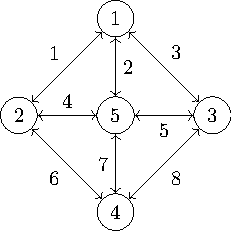
\includegraphics[keepaspectratio,width=1.0\textwidth,height=0.42\textheight]{chapters/tsp/figs/ugraph-figure0}
\caption{\label{fig:tsp:ugraph}Sample weighted graph G with at least one Hamiltonian cycle}
\end{figure}

Consider a digraph G such as that in \cref{fig:tsp:ugraph}.  Ordinarily this would be shown as an undirected graph because all arcs are two-way, but it is presented as an equivalent directed graph so that it more closely matches the input digraphs as described for the \gls{cps} rules described above, specifically regarding the set \(E\) of arc subcells.  A quick examination will show that there is at least one Hamiltonian cycle in this digraph, and thus there will be at least one Hamiltonian cycle with the minimum total weight.  \Cref{fig:tsp:utree} is a tree diagram showing the logical progression of the algorithm as applied to this digraph, assuming that vertex 1 is selected as the root of the Hamiltonian cycle.  Vertices in bold are the ends of the paths with a minimum cost, while vertices in italics are the ends of the paths where there is no arc in the digraph such that a Hamiltonian cycle can be completed, based on the digraph traversal up to that point.  The arcs are labelled with the cumulative weight of the path taken to reach the lower vertex.

\begin{figure}
\centering
% 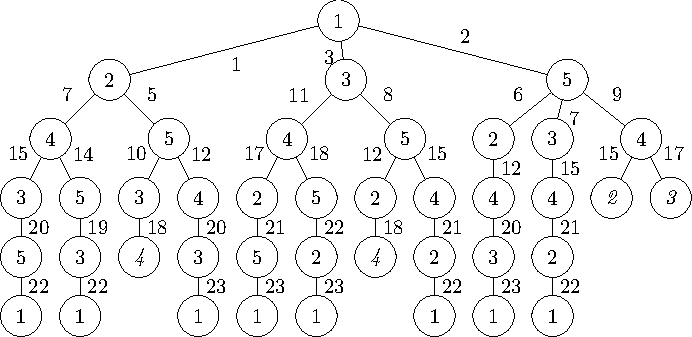
\includegraphics[keepaspectratio,width=1.0\textwidth,height=0.35\textheight]{chapters/tsp/figs/ugraph-figure1}
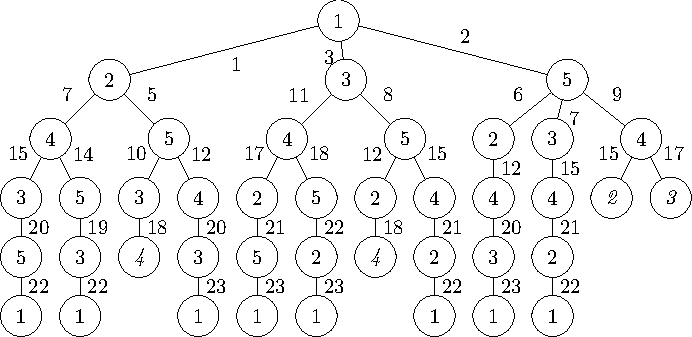
\includegraphics[keepaspectratio,width=1.0\textwidth]{chapters/tsp/figs/ugraph-figure1}
\caption[A tree diagram representing all potential evolutions of the \gls{cps} \glsentrylong{tsp-glossary} algorithm on the graph in \cref{fig:tsp:ugraph}]{\label{fig:tsp:utree}Tree diagram of the \gls{tsp} algorithm in action on graph G}
\end{figure}

\begin{cpobjectsfloat}
\begin{cpobjects}
    \cpobjectsline{\cpfunc{e}{\cpfunc{f}{1}\,\cpfunc{t}{2}\,\cpfunc{w}{1}} \; \cpfunc{e}{\cpfunc{f}{1}\,\cpfunc{t}{3}\,\cpfunc{w}{3}} \; \cpfunc{e}{\cpfunc{f}{1}\,\cpfunc{t}{5}\,\cpfunc{w}{2}} \; \cpfunc{e}{\cpfunc{f}{2}\,\cpfunc{t}{1}\,\cpfunc{w}{1}}}
    
    \cpobjectsline{\cpfunc{e}{\cpfunc{f}{2}\,\cpfunc{t}{4}\,\cpfunc{w}{6}} \; \cpfunc{e}{\cpfunc{f}{2}\,\cpfunc{t}{5}\,\cpfunc{w}{4}} \; \cpfunc{e}{\cpfunc{f}{3}\,\cpfunc{t}{1}\,\cpfunc{w}{3}} \; \cpfunc{e}{\cpfunc{f}{3}\,\cpfunc{t}{4}\,\cpfunc{w}{8}}}
    
    \cpobjectsline{\cpfunc{e}{\cpfunc{f}{3}\,\cpfunc{t}{5}\,\cpfunc{w}{5}} \; \cpfunc{e}{\cpfunc{f}{4}\,\cpfunc{t}{2}\,\cpfunc{w}{6}} \; \cpfunc{e}{\cpfunc{f}{4}\,\cpfunc{t}{3}\,\cpfunc{w}{8}} \; \cpfunc{e}{\cpfunc{f}{4}\,\cpfunc{t}{5}\,\cpfunc{w}{7}}}
    
    \cpobjectsline{\cpfunc{e}{\cpfunc{f}{5}\,\cpfunc{t}{1}\,\cpfunc{w}{2}} \; \cpfunc{e}{\cpfunc{f}{5}\,\cpfunc{t}{2}\,\cpfunc{w}{4}} \; \cpfunc{e}{\cpfunc{f}{5}\,\cpfunc{t}{3}\,\cpfunc{w}{5}} \; \cpfunc{e}{\cpfunc{f}{5}\,\cpfunc{t}{4}\,\cpfunc{w}{7}}}
    
    \cpobjectsline{\cpfunc{v}{\cpfunc{v}{1} \, \cpfunc{v}{2} \, \cpfunc{v}{3} \, \cpfunc{v}{4} \, \cpfunc{v}{5}}}
\end{cpobjects}
\caption[Starting set of subcells from \cref{fig:tsp:utree}]{\label{objs:tsp:obj1}Set of subcells from G in the skin membrane at the initial state}
\end{cpobjectsfloat}

The set of subcells contained inside the membrane at various points in the system's evolution are shown in \crefrange{objs:tsp:obj1}{objs:tsp:obj4} (for legibility, when specifying the \(p\) subcells, \cref{objs:tsp:obj4} adopts the compact presentation style for lists set out in \cref{sec:cps:lists}).  The system starts with the subcells shown in \cref{objs:tsp:obj1}, and the algorithm starts by applying \cpruleref{rule:tsp:tsp:start}, selecting vertex 1 as the starting point of the Hamiltonian cycle and creating the origin subcell \(\cpfunc{s}{\dots}\) (full details of the contents of the subcells are provided in the figures), as shown in \cref{objs:tsp:obj2}.

\begin{cpobjectsfloat}
\begin{cpobjects}
    \cpobjectsline{\cpfunc{e}{\cpfunc{f}{1}\,\cpfunc{t}{2}\,\cpfunc{w}{1}} \quad \cdots \quad \cpfunc{e}{\cpfunc{f}{5} \, \cpfunc{t}{4} \, \cpfunc{w}{7}}}
    \cpobjectsline{\cpfunc{s}{\cpfunc{r}{1} \; \cpfunc{u}{\cpfunc{v}{2} \, \cpfunc{v}{3} \, \cpfunc{v}{4} \cpfunc{v}{5}} \; \cpfunc*{p}{\cpfunc{h}{1} \cpfunc*{p}{\cpempty}} \; \cpfunc{c}{0}}}
\end{cpobjects}
\caption{\label{objs:tsp:obj2}Set of subcells in the skin membrane after the application of rule one}
\end{cpobjectsfloat}

Next, \cpruleref{rule:tsp:tsp:explore} is applied, creating the first level of subcells in the exploration tree.  This creates new \(\cpfunc{s}{\cpfunc{r}{R} \, \cpfunc{u}{\dots} \, \cpfunc{p}{\cpfunc{h}{\dots} \cpfunc*{p}{\cpfunc{h}{1} \cpfunc*{p}{\cpempty}}} \, \cpfunc{c}{\dots}}\) subcells, representing the potential paths of the cycle after one step.  \cpRuleref{rule:tsp:tsp:clean} concurrently removes the old \(s\) subcells from the system.  \Cref{objs:tsp:obj3} shows the subcells within the \gls{tlc} at the end of this first application of Rules \cpruleref*{rule:tsp:tsp:explore} and \cpruleref*{rule:tsp:tsp:clean}.

\begin{cpobjectsfloat}
\begin{cpobjects}
    \cpobjectsline{\cpfunc{e}{\cpfunc{f}{1}\,\cpfunc{t}{2}\,\cpfunc{w}{1}} \quad \cdots \quad \cpfunc{e}{\cpfunc{f}{5} \, \cpfunc{t}{4} \, \cpfunc{w}{7}}}
    \cpobjectsline{\cpfunc{s}{\cpfunc{r}{1} \; \cpfunc{u}{\cpfunc{v}{3} \, \cpfunc{v}{4} \cpfunc{v}{5}} \; \cpfunc{p}{\cpfunc{h}{2} \cpfunc*{p}{\cpfunc{h}{1} \cpfunc*{p}{\cpempty}}} \; \cpfunc{c}{1}}}
    \cpobjectsline{\cpfunc{s}{\cpfunc{r}{1} \; \cpfunc{u}{\cpfunc{v}{2} \, \cpfunc{v}{4} \cpfunc{v}{5}} \; \cpfunc{p}{\cpfunc{h}{3} \cpfunc*{p}{\cpfunc{h}{1} \cpfunc*{p}{\cpempty}}} \; \cpfunc{c}{3}}}
    \cpobjectsline{\cpfunc{s}{\cpfunc{r}{1} \; \cpfunc{u}{\cpfunc{v}{2} \, \cpfunc{v}{3} \cpfunc{v}{4}} \; \cpfunc{p}{\cpfunc{h}{2} \cpfunc*{p}{\cpfunc{h}{5} \cpfunc*{p}{\cpempty}}} \; \cpfunc{c}{2}}}
\end{cpobjects}
\caption{\label{objs:tsp:obj3}Set of subcells in the skin membrane after a single application of rules three and four}
\end{cpobjectsfloat}

Eventually, after repeating \cpruleref*{rule:tsp:tsp:explore} and \cpruleref*{rule:tsp:tsp:clean} four times, \cpruleref{rule:tsp:tsp:makezs} becomes applicable.  At this point, \cpruleref{rule:tsp:tsp:makezs} is applied, creating the \(z\) subcells that represent the final arc traversal from another vertex back to the origin vertex, vertex 1.  Finally, \cpruleref{rule:tsp:tsp:min} selects one of those \(z\) subcells with minimum cost as the solution, and outputs the path and cost subcells relating to that cycle.  \Cref{objs:tsp:obj4} outlines the subcells present in the system at this end point.

\begin{cpobjectsfloat}
\begin{cpobjects}
    \cpobjectsline{\cpfunc{e}{\cpfunc{f}{1}\,\cpfunc{t}{2}\,\cpfunc{w}{1}} \quad \cdots \quad \cpfunc{e}{\cpfunc{f}{5} \, \cpfunc{t}{4} \, \cpfunc{w}{7}}}
    \cpobjectsline{\cpfunc{z}{\cpfunc{c}{22} \; \cpfunc{p}{1|5|3|4|2|1}} \quad \cdots \quad \cpfunc{z}{\cpfunc{c}{22} \; \cpfunc{p}{1|2|4|3|5|1}}}
    \cpobjectsline{\cpfunc{c'}{22} \quad \cpfunc{p'}{1|5|3|4|2|1}}
\end{cpobjects}
\caption[Set of subcells in the skin membrane at completion of the computation]{\label{objs:tsp:obj4}Set of subcells in the skin membrane at completion of the computation, if \cpruleref{rule:tsp:tsp:min} selects the subcell containing the path subcell representing the traversals 1 - 2 - 4 - 3 - 5 - 1.}
\end{cpobjectsfloat}

To illustrate the progression of the algorithm through various branches of the exploration tree, consider the following examples, each beginning with the \(\cpfunc{s}{\ldots}\) and set of \(\cpfunc{e}{\ldots}\) subcells illustrated in \cref{objs:tsp:obj2}.

From \(\cpfunc*{s}{\cpfunc{r}{1}  \,\cpfunc*{u}{\cpfunc{v}{2}\,\cpfunc{v}{3}\,\cpfunc{v}{4}\,\cpfunc{v}{5}}\,  \cpfunc*{p}{\cpfunc{h}{1}\cpfunc{p}{\cpempty}}  \,\cpfunc{c}{0}}\), the subcell representing the beginning of the cycle at vertex 1, \cpruleref{rule:tsp:tsp:explore} will create, among others, an \(\cpfunc*{s}{\cpfunc{r}{1} \; \, \\ \allowdisplaybreaks \cpfunc*{u}{\cpfunc{v}{3} \, \cpfunc{v}{4} \, \cpfunc{v}{5}} \; \, \allowdisplaybreaks \cpfunc*{p}{\cpfunc{h}{2} \cpfunc*{p}{\cpfunc{h}{1} \cpfunc{p}{\cpempty}}} \; \, \allowdisplaybreaks \cpfunc{c}{1}}\) subcell representing an arc traversal to vertex 2 with a weight subcell \(\cpfunc{c}{1}\).  In turn, another new subcell, among others, will be derived from this subcell representing a further arc traversal to vertex 4, with a weight subcell of \(\cpfunc{c}{7}\).  This continues for subcells representing traversals to vertices 3 (\(\cpfunc{c}{15}\)) and 5 (\(\cpfunc{c}{20}\)), until finally the latter subcell contains an empty \(u\) subcell.  For this subcell, \cpruleref{rule:tsp:tsp:makezs} finds an \(e\) subcell that connects vertex 5 to \(R\), the root vertex 1, and so creates a \(z\) subcell (the top \(z\) subcell in \cref{objs:tsp:obj4}) containing a \(\cpfunc{p}{\dots}\) subcell representing the traversed path, and a subcell \(\cpfunc{c}{22}\), representing the total cost of the cycle.  This final subcell is potentially selected at random by \cpruleref{rule:tsp:tsp:min}, because 22 is the minimum cost possible in this particular digraph, when starting and finishing at vertex 1.

Conversely, another chain of subcell creations will occur as vertex 1 to vertex 5, with \(\cpfunc{c}{2}\), vertex 5 to vertex 4 with \(\cpfunc{c}{9}\), vertex 4 to vertex 2 with weight \(\cpfunc{c}{15}\).  At this point, \(\cpfunc{u}{\cpfunc{v}{3}}\) is non-empty, but there is no \(e\) subcell representing a transition from vertex 2 to vertex 3, so this subcell reaches a `dead-end', and will be removed without further effect by \cpruleref{rule:tsp:tsp:clean}.

Similarly, a progression will occur from vertex 1 to vertex 3 with \(\cpfunc{c}{3}\), to vertex 5 with \(\cpfunc{c}{8}\), to vertex 2 with \(\cpfunc{c}{12}\), and to vertex 4 with \(\cpfunc{c}{18}\).  At this point, every vertex has been visited, and the subcell \(u\) in this particular \(s\) subcell is empty, but there is no \(e\) subcell representing a transition from the current vertex back to the origin, so no \(z\) subcell will be created based on it.

%-------------------------------------------

\subsection{Directed Graph Example}
While the above example is drawn as a directed graph, to match better with the specification of the edges in the set of subcells \(E\), it was effectively an undirected graph.  To demonstrate that the \gls{tsp} algorithm is at least as effective in the directed case, \cref{fig:tsp:ugraph} was modified to remove some bidirectional arcs.  The modified digraph is presented in \cref{fig:tsp:digraph} and the accompanying exploration tree in \cref{fig:tsp:dtree}.  The updated set of subcells that are inside the skin membrane at the start of the computation are shown in \cref{objs:tsp:obj1d}.  The changes made are that the edges from 1 to 2 and from 5 to 3 have been removed, and the weights between 1 and 3 and 4 and 5 have been partially modified so that they are different in each direction.

\begin{figure}
\centering
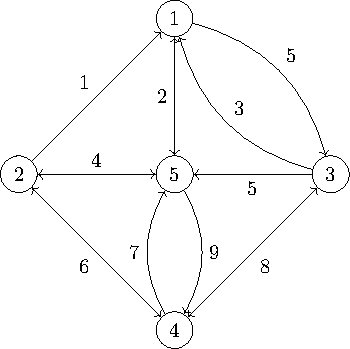
\includegraphics[keepaspectratio,width=1.0\textwidth,height=0.35\textheight]{chapters/tsp/figs/ugraph-figure2}
\caption{\label{fig:tsp:digraph}Sample weighted digraph H with at least one Hamiltonian cycle}
\end{figure}

\begin{figure}
\centering
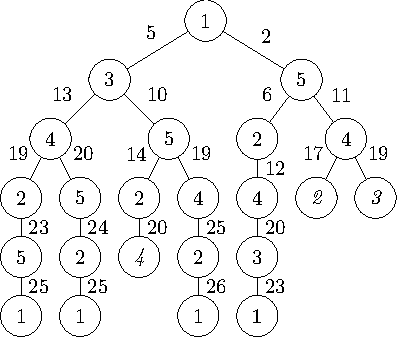
\includegraphics[keepaspectratio,width=1.0\textwidth,height=0.35\textheight]{chapters/tsp/figs/ugraph-figure3}
\caption[Tree diagram of the \glsentrylong{tsp-glossary} algorithm's operation on a directed graph]{\label{fig:tsp:dtree}Tree diagram of the \gls{tsp} algorithm in action on the second, directed graph, H}
\end{figure}

\begin{cpobjectsfloat}
\begin{cpobjects}
    \cpobjectsline{\mathbf{\cpfunc{e}{\mathbf{\cpfunc{f}{1}\,\cpfunc{t}{3}\,\cpfunc{w}{5}}}} \quad \cpfunc{e}{\cpfunc{f}{1}\,\cpfunc{t}{5}\,\cpfunc{w}{2}} \quad \cpfunc{e}{\cpfunc{f}{2}\,\cpfunc{t}{1}\,\cpfunc{w}{1}}}%
    \cpobjectsline{\cpfunc{e}{\cpfunc{f}{2}\,\cpfunc{t}{4}\,\cpfunc{w}{6}} \quad \cpfunc{e}{\cpfunc{f}{2}\,\cpfunc{t}{5}\,\cpfunc{w}{4}} \quad \cpfunc{e}{\cpfunc{f}{3}\,\cpfunc{t}{1}\,\cpfunc{w}{3}} \quad \cpfunc{e}{\cpfunc{f}{3}\,\cpfunc{t}{4}\,\cpfunc{w}{8}}}%
    \cpobjectsline{\cpfunc{e}{\cpfunc{f}{3}\,\cpfunc{t}{5}\,\cpfunc{w}{5}} \quad \cpfunc{e}{\cpfunc{f}{4}\,\cpfunc{t}{2}\,\cpfunc{w}{6}} \quad \cpfunc{e}{\cpfunc{f}{4}\,\cpfunc{t}{3}\,\cpfunc{w}{8}} \quad \cpfunc{e}{\cpfunc{f}{4}\,\cpfunc{t}{5}\,\cpfunc{w}{7}}}%
    \cpobjectsline{\cpfunc{e}{\cpfunc{f}{5}\,\cpfunc{t}{1}\,\cpfunc{w}{2}} \quad \cpfunc{e}{\cpfunc{f}{5}\,\cpfunc{t}{2}\,\cpfunc{w}{4}} \quad \mathbf{\cpfunc{e}{\mathbf{\cpfunc{f}{5}\,\cpfunc{t}{4}\,\cpfunc{w}{9}}}}}%
    \cpobjectsline{\cpfunc{v}{\cpfunc{v}{1} \, \cpfunc{v}{2} \, \cpfunc{v}{3} \, \cpfunc{v}{4} \, \cpfunc{v}{5}}}
\end{cpobjects}
    \caption[Set of subcells from H in the skin membrane at the initial state]{\label{objs:tsp:obj1d}Set of subcells from H in the skin membrane at the initial state (those different from G are in bold)}
\end{cpobjectsfloat}

These modifications have a significant effect upon the evolution of the system.  There are fewer potential paths through the digraph, which results in the instantiation of fewer subcells, and so the exploration tree is consequently narrower.  Thus, this particular application of the algorithm has a lower maximum space complexity.  Note though that there is absolutely no change in the operation of the algorithm.  The differences in the \(e\) subcells present at the start of the evolution of the system lead to a different result, without any change in the application of the rules.

%----------------------------------------
\section{\label{sect:variations}Variations on the Algorithms}
We have presented above algorithms to find a single Hamiltonian path or cycle, with minimum cost in the case of a weighted digraph (i.e., the \gls{tsp}).  With minimal modifications however, other results may be obtained from the algorithm, such as using a specific starting vertex or generating all possible paths/cycles.

To use a specific vertex as the starting point of the algorithm, rule (1) may be skipped by starting the system in state 2, with an \(s\) subcell containing the chosen vertex as the head of the \(p\) subcell supplied to the top-level cell.

For the \gls{hcp} and \gls{tsp}, rule (5) could be applied in \(\mathtt{max}\) mode without any other changes so as to produce all possible Hamiltonian cycles (with minimum cost for the \gls{tsp}) back to the starting node.  This results in the output into the top-level cell of multiple \(p'\) subcells, to be handled further as appropriate.  The same modification can be applied to rule (5) of the \gls{tsp} algorithm to obtain all minimum-cost cycle paths.  Likewise for each problem, if \(\mathtt{max}\) mode is used on rule (1), then the paths/cycles starting at every vertex will be generated.  These all potentially have the effect of increasing the space complexity of the system, which is not an issue for P~systems with their infinite available space, but may impact software simulations.

%In the case of a Hamiltonian path, more interesting is if a particular vertex is desired as the end point of the system.

% For the \gls{hcp} and \gls{tsp}, a specific vertex can be required as the ending point of the cycle.  This requires the instantiation of two extra unique subcells, which we will name here \(j\) and \(k\), shown in \autoref{hcprule12alt}.  Such a subcell is created either in the top-level cell at the time of application of rule (1), or supplied inside an initial \(s\) subcell.  Rule (2) of the \gls{hcp} or \gls{tsp} rules is modified so that instead of seeking \(e\) subcells that point back to the origin vertex, it instead instantiates the \(z\) subcells based on connections to the terminus vertex.  

% \begin{figure}[!htbp]
% \begin{framed}
% \renewcommand{\arraystretch}{1.5}
% \[\begin{array}{lllr}
% S_1 ~ & ~ v(v(R)v(N)Y) & \rightarrow_{1} ~ S_2 ~~ s(u(Y) ~ n(N) ~ p(h(R)p())) ~ & \qquad (1) \\
% S_2 ~ & ~   ~ &   \rightarrow_{1} ~ S_3 ~ p'(h(N)P)  & \qquad (2) \\
% 	~ & ~	~ & ~ \hspace{1.5cm} ~ | ~ s(u() ~ n(N) ~ p(h(N)P))	\\
% \end{array}\]
% \end{framed}
% \caption{Alternative rules 1 and 2 for the \gls{hcp} \& \gls{tsp} algorithms for finding cycles that end at a given vertex}
% \label{hcprule12alt}  
% \end{figure}

% For the \gls{hcp}, if all possible Hamiltonian cycles from the starting node are desired, rule (5) could instead be applied in \(\mathtt{max}\) mode without any other changes to achieve the desired result %, as shown in \autoref{hcprule5alt}
% -- this of course also applies to the \gls{hpp} rules.  This results in the output into the top-level cell of multiple \(p\) subcells, to be handled further as appropriate.
% %  Or rule (5) can leave the system in state \(S_3\), in which case the rule is applied ad infinitum, producing a path subcell at random from the collection of created subcells.  %Differently again, rule 5 could be modified so that it destroys the \(z\) subcell it selects instead of using it as a promoter, and thus the computation eventually terminates as all the generated \(z\) subcells are used up, but that appears to be simply a less efficient alternative to using \(\mathtt{max}\) mode.  
% The same modification can be applied to rule (5) of the \gls{tsp} algorithm to obtain all minimum-cost cycle paths.  Likewise, if \(\mathtt{max}\) mode is used on rule (1), then the paths/cycles starting at every vertex will be generated.

% \begin{figure}[!htbp]
% \begin{framed}
% \renewcommand{\arraystretch}{1.5}
% \[\begin{array}{lllr}
% S_3 ~ & ~   ~ & \rightarrow_{+} ~ S_4 ~ p'(P))   & \qquad \qquad (5b) \\
% 	~ & ~	~ & ~ \hspace{1.5cm} ~ | ~ z(p(P))	\\
% \end{array}\]
% \end{framed}
% \caption{Alternative rule 5 for the \gls{hcp} algorithm returning all Hamiltonian paths from a given starting node}
% \label{hcprule5alt}  
% \end{figure}

%Furthermore, if all possible Hamiltonian cycles from \textbf{every} node of the graph are desired, the only change required to achieve this is to modify rule (1) so that it operates in \(\mathtt{max}\) mode, rather than \(\mathtt{min}\) mode.  This would generate a starting \(s\) subcell carrying an \(r\) root subcell for every node in the graph, because the unification of \(R\) described in the rule will match upon every node contained in the initial \(v\) subcell.  Neither this change nor the alternative \(\mathtt{max}\)-mode rule (5) described above impact the running time of the algorithm -- though they will increase the space requirements to a greater or lesser degree, which has no effect in P~systems with their infinite available space, but may impact computerised simulations of them.

In \autoref{sect:algotsp} we assumed that all arc weights are strictly positive integers.  Weights of zero can be accommodated relatively easily.  Should every possible cycle have a minimum weight of at least 1, then no changes are needed.  If it is possible for there to be a cycle with a total weight of zero, then a sixth rule must be introduced, prior to the current rule (5), which in turn becomes rule (6).  This rule simply detects a minimum of zero, as set out in \autoref{sec-min}.  These new rules are shown in \autoref{minzerorules} (recall that \(\lambda\) inside a subcell denotes the subcell as empty).

% \begin{figure}[htbp]
% \begin{framed}
% %\begin{adjustwidth}{-1em}{-1em}
% \renewcommand{\arraystretch}{1.5}
% \[\begin{array}{lllr}
% % S_3 ~ & ~   ~ & \rightarrow_{1} ~ S_4 ~ p'(P) ~~~ c'(\lambda)  & (5) \\
% %     ~ & ~   ~ & ~ \hspace{1.5cm} ~ | ~ z(p(P) ~ c(\lambda)) \\
% % S_3 ~ & ~   ~ & \rightarrow_{1} ~ S_4 ~ p'(P) ~~~ c'(C1W)   & (6) \\
% % 	~ & ~	~ & ~ \hspace{1.5cm} ~ | ~ z(p(P) ~ c(C1W))	\\
% %     ~ & ~	~ & ~ \hspace{1.5cm} ~ \neg ~ z(p(\_) ~ c(C))	\\
% S_3 ~ & ~   ~ & \rightarrow_{1} ~ S_4 ~ p'(P) ~~~ c'(\lambda)  & (5) \\
%     ~ & ~   ~ & ~ \hspace{1.5cm} ~ | ~ z(p(P) ~ c(\lambda)) \\
% S_3 ~ & ~   ~ & \rightarrow_{1} ~ S_4 ~ p'(P) ~~~ c'(1D)   & (6) \\
% 	~ & ~	~ & ~ \hspace{1.5cm} ~ | ~ z(p(P) ~ c(1D))	\\
%     ~ & ~	~ & ~ \hspace{1.5cm} ~ \neg ~ (D = CW) ~ z(p(\_) ~ c(C))	\\
% \end{array}\]
% %\end{adjustwidth}
% \end{framed}
% \caption{Rules to find the minimum cost path in our \gls{tsp} algorithm, when that path cost may be zero}
% \label{minzerorules}  
% \end{figure}

\changerulenumber{4}

\begin{cprulesetfloat}
\begin{cpruleset}
    \cprule{s_3}{}{1}{s_4}{\cpfunc{p'}{P} \; \cpfunc{c'}{\cpempty}}
    \cppromoter{\cpfunc{z}{\cpfunc{p}{P} \, \cpfunc{c}{\cpempty}}}
    
    \cprule{s_3}{}{1}{s_4}{\cpfunc{p'}{P} \; \cpfunc{c'}{C \cpundig W}}
    \cppromoter{\cpfunc{z}{\cpfunc{p}{P} \, \cpfunc{c}{C \cpundig W}}}
    \cpinhibitor{\cpfunc{z}{\cpfunc{p}{\_} \, \cpfunc{c}{C}}}
    
\end{cpruleset}
\caption{\label{minzerorules} Rules to find the minimum cost path in our \gls{tsp} algorithm, when that path cost may be zero}
\end{cprulesetfloat}
\section{\label{sec:tsp:conc}Summary}
This chapter defined a succinct \gls{cps} algorithm for solving the \gls{tsp} in \bigoh{n} time, by using the capacity of \gls{cps} to create and manipulate complex subcells in only a few high-level steps.  This algorithm builds on a simpler version for finding Hamiltonian Paths and Cycles, requires only a fixed set of five rules, and takes \(n + 3\) steps to find a solution for any connected digraph of size \(n\), an improvement on the previous best known \gls{ps}-based solution to the \gls{tsp}.

Simple examples were provided to demonstrate the operation of the algorithm.  The \gls{tsp} algorithm can operate, without modification to the \gls{ruleset}, on any arbitrary weighted graph with a Hamiltonian Cycle.   The algorithm requires only a specification of the graph encoded as subcells, and could be extended to detect the absence of a Hamiltonian Cycle.

\begin{table}[htb]
\centering
\caption{Comparison of known exact \gls{ps} solutions to the \glsxtrlong{tsp}}
\label{tab:tsp:algocomp}
\setlength{\tabcolsep}{5pt}
\begin{tabular}{@{}lcc@{}}
\toprule
\textbf{Algorithm}  & \multicolumn{1}{l}{\textbf{\begin{tabular}[c]{@{}c@{}}Num. of\\  rules\end{tabular}}} & \multicolumn{1}{l}{\textbf{\begin{tabular}[c]{@{}c@{}}Run time\\  order\end{tabular}}} \\ \midrule
Guo \& Dai \cite{Guo2017}          & $\sim$50                                   & \bigoh{n^2}                                         \\
Cooper \& Nicolescu & 5                                          & \bigoh{n}                                          \\ \bottomrule
\end{tabular}
\end{table}

%-------------------------------------------------

% \begin{appendix}
\section{\label{sec:tsp:simulation}Simulations}
To demonstrate that this approach can be applied in practice to small problem graphs, sample simulations were written in SWI-Prolog, \fsharp{} and Erlang for the \gls{tsp} algorithm.  In each case, the programs were written with an emphasis on matching the \gls{cps} algorithm, rather than with a focus on memory or time efficiency.  Better implementations from a real-world-use viewpoint could likely be created, but they may not reflect the \gls{cps} rules quite as well.  The Prolog program in particular matches very closely to the \gls{cps} algorithm, and so is fully presented here.  A complete program listing for the Prolog program's rules corresponding to the algorithm is in \cref{app:tsp:codeprolog}, while \cref{app:tsp:probprolog} defines the problem graph.  A copy of the source code for each simulation is available at \url{https://github.com/jcoo092/cP-Systems-TSP}.  While care was taken to keep these simulations similar to each other, differences between the languages inevitably means they are not identical.

All three languages are reasonably well-suited to implementing \gls{cps}.  As mentioned, the Prolog program in particular maps well to the algorithm, requiring only 7 Prolog rules in total, plus a variable number of facts specifying the problem graph, 17 in this case.  The functional elements of \fsharp{} such as higher-order functions also allow a reasonable approximation, if perhaps not with quite the fidelity of Prolog.  Erlang, possibly owing to the fact it was originally implemented atop Prolog, appears to fall in between the two approaches, leaning more towards the functional side.  It is clear from these programs that there is at least one potential close mapping from \gls{cps} to both logic and functional programming languages.  The emphasis here, however, was on demonstrating the similarities of the languages to \gls{cps}, and not on performance.  As such, no attempt has been made to optimise the simulations.

To gauge their `real-world' effectiveness, the simulations were informally tested with increasing digraph sizes.  All three ably coped with digraph sizes of up to 10 vertices, returning an answer at most in a matter of a few seconds.  \fsharp{} and Erlang struggled somewhat at 11 vertices, with the latter taking more than one minute to complete, while Prolog quickly failed with an ``out-of-stack-memory'' error.  The \fsharp{} simulation was tested on a digraph of size 12, but the test was terminated after 90 minutes running time due to time constraints, failing to complete and return a minimum cost path.  Due to this, a 12 vertex run was not attempted with Erlang.

Considering that for a totally connected 11 vertex digraph, at the 11th step almost 40 million (\(11!\)) subcells would be required, it is unsurprising that memory limits may become an issue.  These results suggest that, while the fundamental process does indeed lead to determining lowest-cost paths, much more effective use of memory will be required to make software simulations practical for highly connected digraphs of any significant size (i.e. greater than approximately 11 or 12 vertices).

A comparison of \cref{fig:tsp:utree,fig:tsp:dtree} suggests, however, that for graphs that are not totally connected, the implementations may cope much better, as would be expected.  With ultimately fewer paths to explore, the growth in the number of objects will be lesser, and thus the space requirements will be lowered.  This is not unique by any means to the \gls{cps} version of the \gls{tsp} - any method to solve the \gls{tsp} which involves a breadth-first search of the graph, considering whether nodes have already been visited, will experience the same. 

\subsection{Prolog simulation}

It is perhaps interesting to contrast the Prolog method for exploring the problem space and finding an answer with that of \gls{cps}.  On the surface they appear quite similar -- a handful of rules and some initial statements specific to the problem, combined with unification.   In some ways, however, they appear also to be opposing duals of each other.  Prolog in general, and thus in the case of this program, works on a top-down backward-chaining approach, whilst \gls{cps} works on a bottom-up forward-chaining approach.

That is to say that (sequential) Prolog tries to do the least work and use the least space possible, so it starts with the definition of the requested inference (an invocation of \texttt{go} in the program), and only evaluates elements of that definition as it discovers they are needed in order to provide a result.  In the case of the digraph exploration, this essentially means that it tries to perform a linear depth-first search of the digraph, stopping as soon as it has an answer --- though with the \gls{tsp} it inevitably must evaluate every cycle to know which has minimum cost.

Conversely, the \gls{cps} algorithm starts with the definition of the problem graph, and does all possible work in order to find the result in what is essentially a breadth-first search.  All possible cycles from the root node are instantiated and eventually checked for minimum cost. The ability of \gls{cps} to perform these instantiations and the comparison completely in parallel means that a relatively small number of steps are required to find the minimum -- though at the cost of a potentially (exponentially) large space and processing complexity.

\begin{listing}
\caption{\label{app:tsp:probprolog}SWI-Prolog code defining the example problem undirected graph G shown in \cref{fig:tsp:ugraph}}
\inputminted[linenos,breaklines,frame=lines,autogobble,lastline=3]{prolog}{chapters/tsp/code/tsp.pl.txt}
\end{listing}

\begin{listing}
\caption[Complete SWI-Prolog code for the \acrlong{tsp} algorithm]{\label{app:tsp:codeprolog}Complete SWI-Prolog code for the rules of the \gls{tsp} algorithm}
\inputminted[linenos,breaklines,frame=lines,autogobble,firstline=5]{prolog}{chapters/tsp/code/tsp.pl.txt}
\end{listing}
% \end{appendix}

\glsresetall
\newcommand{\bo}{\(b\)}

\chapter{\label{chap:gcol}The \glsfmtname{gcp-glossary}}

The \gls{gcp} is a deceptively simple problem in graph theory.  In its most basic form, it is the problem of assigning labels such as colours to the nodes in a graph so that no two nodes connected by an edge share a colour, usually with the addition of the extra requirement either of finding the minimum number of colours required or only using a number of colours up to some upper bound --- of course, for any graph with \(N\) nodes, it is trivial to colour it as required using \(N\) colours.  The problem finds applications in many areas, including timetabling, register allocation for compilers, as well as solving Sudoku puzzles (which are in turn a special case of Latin Squares) \cite{Lewis2016}.  The general case is NP-Complete, and thus no polynomial time solution has been found so far (finding one would prove that P = NP), though they have been found for specific forms of graph or particular numbers of colours.  For example, in the case of 3-colouring, the current best known solution takes \bigoh{1.3289^n} time \cite{Beigel2005}.

\citeauthor{Gheorghe2013} presented a \gls{ps} solution to the 3-colouring problem, using communicating \gls{skps} \cite{Gheorghe2013}.  Based on this work, this \namecref{chap:gcol} first discusses in \cref{sec:gcol:cml} a \gls{cml} implementation of the \gls{skps} solution in \cite{Gheorghe2013}, briefly compares the two approaches and indicates some other \gls{ps} variants which \gls{cml} might be a good fit with.  This \namecref{chap:gcol} then presents in \cref{sec:gcol:cpsys} a concise single-cell solution to the problem using \gls{cps}, and provides an informal analysis of it.  Lastly, in \cref{sec:gcol:examples}, this \namecref{chap:gcol} provides examples of the operation of the \glspl{cps} on the 3-colour problem, both for a graph that is colourable and one that is not, before summing up in \cref{sec:gcol:conc}.

\section[Simple Kernel P Systems Solution to the \glsfmtname{gcp-glossary} in \glsfmtname{cml-glossary}][\Gls{skps} Solution to the \gls{gcp} in \gls{cml}]{\label{sec:gcol:cml}Simple Kernel P Systems Solution to the \glsfmtlong{gcp-glossary} in \glsfmtlong{cml-glossary}}

This \namecref{sec:gcol:cml} explores \gls{cml} as another methodology to use for simulating \gls{ps} where communication is involved.  For a first experiment, it implements \citeauthor{Gheorghe2013}'s 3-colouring problem solution from \cite{Gheorghe2013}, as it involves communication between \glspl{compartment} but is relatively low-complexity and thus appears to be suitable for a first attempt at simulating communicating \gls{ps} with \gls{cml}.

The programming language \fsharp{} was used with the library Hopac,\footnote{\url{https://github.com/Hopac/Hopac}} which is modelled on \gls{cml} and follows it closely.\footnote{The final program can be found at \url{https://github.com/jcoo092/acmc2018}}  `Record' types are used to represent the individual \glspl{compartment} described in \cite{Gheorghe2013}.  The program then advances through multiple steps, applying the rules (encoded as functions that operate on the record types) in accordance with \cite{Gheorghe2013}.  Finally, once a solution is found, or found not to be possible, that is communicated to the environment.

Insofar as possible, the implementation follows the algorithm described in \cite{Gheorghe2013} faithfully, and thus perhaps is not optimal in its efficiency, as an idiomatic specification of a Simple Kernel P~system does not necessarily match to the idiomatic or efficient form of an \fsharp{} program.  That is, the program prioritises staying as close to the original \gls{skps} model as possible, rather than adapting to suit the strengths and typical style of \fsharp{}.  Consequently, the efficiency of the program may be worse than it could be otherwise.

\subsection{Simulation Results}
The program's running time on a number of differing graphs were recorded, with red, green and blue as the set of colours with which to colour the graphs.  The desktop computer used for these simulations has a four-core \qty{3.6}{\giga\hertz} Intel Core\textsuperscript{\textregistered} i7-7700 CPU, with \qty{16}{\gibi\byte} of RAM, running Windows 10, build number 10.0.17134.228.  The \fsharp{} programs were compiled and run on .NET Core 2.1.4, while \gls{mecosim} was run on Java version 8, build 1.8.0\_201-b09.

The first simulation used the graph shown in Figure 2 of \cite{Gheorghe2013}, reproduced here as \cref{fig:gcol:gheorghefig2}, which took \qty{2.6}{\second} to process.  In keeping with that paper and following its definition of \(G(N,q)\), where \(G(N,q)\) is used to represent a graph of \(N\) nodes with all other nodes connected only to node \(q\) in a hub-and-spoke formation,\footnote{This is different to the random graphs that are also commonly denoted by this notation.} the graphs \(G(10,1)\) and \(G(10,10)\) (see \cref{fig:gcol:gs}) were also tested, finding that \qty{0.3}{\second} is required for each.  The simulation was also tested using the classic \emph{Petersen graph}, shown in \cref{fig:gcol:petersen}, and found that it too required approximately \qty{0.3}{\second}.

\begin{figure}
    \centering
    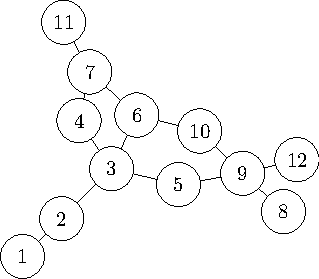
\includegraphics[width=0.65\textwidth]{chapters/gcol/figs/gheorghe-figure-2-figure0.pdf}
    \caption[A reproduction of the graph in Figure 2 of \cite{Gheorghe2013}]{\label{fig:gcol:gheorghefig2}A reproduction of Figure 2 from \cite{Gheorghe2013}.  Although this figure and Figure 2 in \cite{Gheorghe2013} are visually distinct, the graphs are isomorphic.}
\end{figure}

\begin{figure}
    \centering
    \begin{subfigure}[b]{0.35\textwidth}
        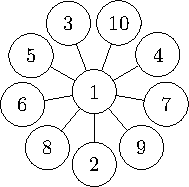
\includegraphics[width=\textwidth]{chapters/gcol/figs/g-10-1.pdf}
        \caption{\label{fig:gcol:g-10-1}\(G(10,1)\)}
    \end{subfigure}
    \hfill
    \begin{subfigure}[b]{0.35\textwidth}
        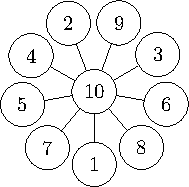
\includegraphics[width=\textwidth]{chapters/gcol/figs/g-10-10.pdf}
        \caption{\label{fig:gcol:g-10-10}\(G(10,10)\)}
    \end{subfigure}
    \caption[Graphs representing \(G(10,1)\) and \(G(10,10)\)]{\label{fig:gcol:gs}Graphs representing (a) \(G(10,1)\) and (b) \(G(10,10)\), as described in \cite{Gheorghe2013}, where the first number represents the size of the graph, and the second number represents the label of the centre node of the graph, with all other nodes connected only to that node.}
\end{figure}

\begin{figure}
    \centering
    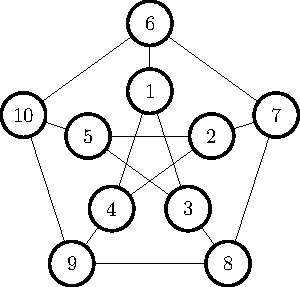
\includegraphics[width=0.45\textwidth]{chapters/gcol/figs/petersen-figure0.pdf}
    \caption[The Petersen Graph]{\label{fig:gcol:petersen}The classic Petersen graph, with nodes labelled 1 to 10.}
\end{figure}

Further simulations were run on complete graphs.  For a complete graph of \(N = 10\), the algorithm again required \qty{0.3}{\second}.  It was then tried on a complete graph of \(N = 20\), but the test had to be aborted after a matter of minutes due to the computer running out of memory.  Running times of \qty{0.83}{\second}, \qty{2.6}{\second}, \qty{8.88}{\second}, \qty{26.6}{\second} and \qty{84}{\second} for \(N = 11, 12, 13, 14\) and \(15\), respectively, were recorded.  Given that significant jumps in memory use were observed while running the larger graphs, it appears that the major cause of the rapid slowdown is likely to do with frequent \adhoc{} memory allocations and de-allocations, though this was not profiled in detail.

\citeauthor{Gheorghe2013} state \cite[p.~828]{Gheorghe2013} that in the latest version of \gls{plingua} at the time of writing, a strategy of eliminating \glspl{compartment} for which there can be no further rule applications is employed.  Using said strategy, results are typically achieved quite quickly.  It has the effect of pruning the search space, and reduces the total running time in some instances to just one-fifth of the running time of the simulation without such dead-\gls{compartment}-elimination.

The \fsharp{} program does not choose which \glspl{compartment} to operate upon in the same fashion, but applying the colour guard on rule \(r_{2,2n+1}\) of the \gls{skps}~system throughout the process results in the pruning of \glspl{compartment} which already contain invalid results and thus can be eliminated safely. Therefore, to achieve the same effect as with \gls{plingua}'s strategy, this guard was used while applying rule \(r_{2,2n+1}\) and the result used to filter out all invalid \glspl{compartment}.  Doing this reduces the evaluation of complete graphs to around 60 milliseconds or slightly more, since every \gls{compartment} in them can always be eliminated once colours have been assigned to four nodes.  It also reduces the running time of \cref{fig:gcol:gheorghefig2} to around \qty{0.25}{\second}, and the Petersen graph, \(G(10,1)\) and \(G(10,10)\) to \qty{0.1}{\second}.

\subsubsection{Comparison with Original Results}

\Cref{tab:gcol:timings} compares the timing results of the simulations reported in \cite{Gheorghe2013}, as well as the results of using \gls{mecosim}\footnote{The latest version of \gls{mecosim} available from \url{http://www.p-lingua.org/mecosim/} as at 10 January 2019 was used.} \cite{Perez-Hurtado2010} to re-run the same simulations locally on the same computer used to time the \fsharp{} solution, with the timing results mentioned above.

\begin{table}
\centering
\begin{tabular}{@{}lcccc@{}}
\toprule
Graph       & \begin{tabular}[c]{@{}c@{}}\gls{plingua}\\ (original)\end{tabular} & \begin{tabular}[c]{@{}c@{}}\gls{plingua}\\ (local)\end{tabular} & CML   & \begin{tabular}[c]{@{}c@{}}CML with\\ pruning\end{tabular} \\ \midrule
Fig. 2 in \cite{Gheorghe2013}      & N/A                                                           & 17.0                                                           & 2.6  & 0.25                                                 \\
Petersen    & N/A                                                           & 1.5                                                       & 0.3  & 0.1                                                       \\
G(10,1)     & 7                                                            & 2.6                                                           & 0.3  & 0.1                                                       \\
G(10,10)    & \textgreater 4 min                             & N/A                                                           & 0.3  & 0.1                                                       \\
Complete 11 & 5                                                            & 0.15                                                           & 0.83 & .06                                                       \\
Complete 12 & 5                                                            & 0.15                                                           & 2.6  & .06                                                       \\
Complete 13 & 5                                                            & 0.15                                                           & 8.88 & .06                                                       \\
Complete 14 & 5                                                            & 0.15                                                           & 26.6 & .06                                                       \\
Complete 15 & 5                                                            & 0.15                                                           & 84   & .06                                                       \\ \bottomrule
\end{tabular}%
\caption[Comparison of recorded timings between \cite{Gheorghe2013} and this work]{Comparison of recorded timings between \cite{Gheorghe2013} and this work.  All measurements are in seconds, unless otherwise stated.  Where more than one result was reported in \cite{Gheorghe2013} for the same graph, the shortest running time has been included here.}
\label{tab:gcol:timings}
\end{table}

Attempts to run the simulation of \(G(10,10)\) in \gls{mecosim} repeatedly failed with an out-of-memory error.  Why this should be the case is uncertain, given that in the other instances, executions of the \gls{mecosim} \gls{skps} simulations achieved lower runtimes than those of \cite{Gheorghe2013}.  The execution of \(G(10,10)\) notwithstanding, the overall improvements in runtime of the \glspl{skps} are likely due to a combination of the computer used locally being more recent and thus likely more powerful, and improvements in the underlying \gls{mecosim} and \gls{plingua} software.

It seems odd, however, that two functionally identical graphs, \(G(10,1)\) and \(G(10,10)\), would have such dramatically different run time behaviours when running in \gls{mecosim} --- seen in both the original and reproduced local results.  This might be due to an unusual performance bug hidden deep within \gls{mecosim}, though this was not investigated further.

These results appear to suggest that the \fsharp{} implementation generally provides superior running time results, though it was not tested on a particularly wide variety of scenarios.  Extrapolating from the collected results, it seems plausible that the scenarios that would result in the longest running time will likely be those that have a moderate level of connectedness in the graph.  Highly connected graphs will likely see many potential paths eliminated early due to frequent occurrences of colour conflicts, while graphs with few connections will have relatively few potential paths to explore.

The \fsharp{} results and those of the \gls{mecosim} simulations are not \emph{completely} comparable, however.  The \fsharp{} solution was programmed directly to follow the \gls{skps} system's rules, whereas the \gls{mecosim} solution was specified as the \gls{skps}~system rules in \gls{plingua}, with the operation of the computer simulation carried out by \gls{mecosim}.  This difference between `\adhoc{}' and `general' simulation means that one would expect to see the \fsharp{} simulation achieve better results from the outset, as overheads that accompany a general simulation implementation can be avoided.\footnote{One could see \adhoc{} as being akin to running a program compiled to native instructions, whereas using a general simulation is similar, in principle, to running a program in an interpreter.  The latter is typically simpler to work with and more portable, but comes with overheads that slow down execution.}  \Gls{mecosim} is an excellent tool, and, combined with \gls{plingua}, it provides a valuable service to the \gls{mc} community in that it allows researchers to validate their systems and \glspl{ruleset} while staying close to their mathematical descriptions, and without having to delve into the details of implementing a given algorithm in code.  See further \cite{Perez-Hurtado2019} for more of a discussion on \adhoc{} and general simulations, and a narrowing of the differences between the two.

Ultimately, this example is relatively trivial and involves little communication, and therefore does not test the use of \gls{cml} significantly.  Much of the operation of the algorithm in fact does not involve communication between different \glspl{compartment}/processing elements at all.  Instead, it is primarily based in the evolution of objects contained within the \glspl{compartment}, with minimal communication between \glspl{compartment} at the end.  While that is highly effective in \gls{ps} \cite{Paun2008}, it would be interesting to see the results of using \gls{cml} for other problems where synchronous communication\footnote{While \gls{cml} uses synchronous communication by default, it is also relatively simple to implement asynchronous communication also using it if desired \cite{Reppy2007}.} is a much bigger part of the evolution of the system.  The experimental results in \cref{chap:median} go some way to investigating this.

In common with most \adhoc{} simulations, while the implementation is reasonably successful, it is not particularly customisable, and the code as written does not comport as precisely to the appearance of the theoretical rules of the \gls{skps}~system as the \gls{plingua} version created for \cite{Gheorghe2013} does.  Neither does the current implementation have any form of verification or invariant detection, as provided by \gls{mecosim} \cite{Perez-Hurtado2010} and Spin \cite{Ben-Ari2008,Lefticaru2011}.

\gls{cml} seems to match to \gls{skps} well, but also looks like it might fit well with \gls{tlps} with symport/antiport \cite{Verlan2005} as well perhaps as \gls{tlps} with Channel States \cite{Song2016}, and Generalized Communicating \gls{ps} with minimal interaction rules \cite{Csuhaj-Varju2011}.  It would also appear to be a good fit for \gls{snps} \cite{Ionescu2006}, though \gls{cml} would probably be `overkill' for \gls{snps}.  In general, any variant of \gls{ps} which heavily uses synchronous communication between different cells/neurons/non-nested membranes/etc. over well-defined channels may be amenable to a \gls{cml} implementation.

Technically, the base form of \gls{cml} would only support symport (\ie{} one-way synchronous communication), but it is fairly simple to build two-way communication on top of it \cite[ch.~6]{Reppy2007}.  No attempt to model other systems has been made yet, however.
\section{\label{sec:gcol:cpsys}\glsentrytext{cps} solution to the \glsentrytext{gcp}}
In the \gls{cml} simulation of the problem, most of the work, in fact, is performed by the instantiation of new objects, rather than communication.  Thus, the problem appears to be an excellent fit to the pre-existing formulation of \gls{cps} \cite{Nicolescu2018}.

This solution assumes a graph with at most one edge between nodes (i.e. there are not two or more edges between the same two nodes), and that there are no edges leading from a node back to itself.  Further, it takes as given inputs to the process conceptual finite sets \(V \subset \mathbb{N}\) representing the nodes of the graph\footnote{In fact, any finite set of arbitrary symbols could be used, but this discussion is restricted to the natural numbers for ease of reading.}; \(E \subseteq \{(i,j)~|~i, j \in V, i \neq j \}\) representing the edges of the graph; and \(K\) representing the chosen colours, where \(K\) contains whatever representation of the desired colours is considered appropriate.

Based on these definitions, for the purposes of the remainder of this \namecref{chap:gcol}, \(|K|\) is defined to be the number of colours used in the current problem, \(|V|\) the number of nodes in the graph under consideration for the current problem and \(|E|\) the number of edges in the graph.

\subsection{Pseudocode for our parallel algorithm}
The logical operation of the system, as carried out using the rules described in detail at \cref{sec:gcol:rules}, can be demonstrated with a pseudocode representation, as shown in \cref{code:gcol:graphcol}.

% \begin{algorithm}
% \DontPrintSemicolon
% \SetKwFunction{Choose}{choose}
% \SetKwFunction{Dom}{Dom}
% \SetKwFunction{Graphcolouring}{Graph Colouring}
% \KwIn{\(V\), \(E\), \(K\)}
% \KwOut{A valid colouring, or an indication no valid colouring is possible}
% \Begin{
% \Choose{\(s \in V\), \(c \in K\)}\;
% \KwRet{\Graphcolouring{\(V\), \(E\), \(K\), \(1\), \(\{\{(s, c)\}\}\)}} \label{li:gcol:endofsmaller}
% }

% \hrulefill

% \KwIn{\(V\), \(E\), \(K\), \(i\), \(B\)}
% \KwOut{A valid colouring, or an indication no valid colouring is possible}
% \Begin{
% \If{\label{li:gcol:iflgreaterthanv} \(i = |V|\)} {
%     \Choose{\(m \in B\)}\;
%     \KwRet{\(m\)}    \label{li:gcol:returnsuccess}
% }
% \(B' \gets \emptyset\)\;
% \For{ \(m \in B,~x \in \Dom{m},~y \in V \setminus \Dom{m},~ d \in K \)}{    \label{li:gcol:makebstart}
%     \If{\((x,y) \in E ~ \land \not\exists(x',y) \in E,~(x',d) \in m\)}{
%         \(B' \gets B' \cup \{m \cup \{ (y,d) \} \}\)\;   \label{li:gcol:makebfinish}
%     }
% }
% \eIf{ \label{li:gcol:fail1} \(B' = \emptyset\) }
%   {
%         \KwRet{\(\emptyset\)}  \label{li:gcol:fail2}}
%     {
%         \KwRet{\Graphcolouring{\(V\), \(E\), \(K\), \(i + 1\), \(B'\)}\label{li:gcol:recurse}}
% }}
% \caption[Pseudocode representation of the algorithm performed by the \glspl{cps} rules in \cref{ruleset:gcol:rules}]{\label{code:gcol:graphcol}Pseudocode representation of the algorithm performed by the \glspl{cps} rules in \cref{ruleset:gcol:rules}.  This employs a doubly defined tail-recursive function approach, where the algorithm begins with the upper function supplied only with the details of the graph and colours, but uses the lower function with further arguments to perform most of the processing.}
% \end{algorithm}

\begin{algorithm}
\DontPrintSemicolon
\SetKwFunction{Choose}{choose}
\SetKwFunction{Dom}{Dom}
\SetKwFunction{Graphcolouring}{Graph Colouring}
\KwIn{\(V\), \(E\), \(K\)}
\KwOut{A valid colouring, or an indication no valid colouring is possible}
\Begin{
\Choose{\(s \in V\), \(c \in K\)}\;
\KwRet{\Graphcolouring{\(V\), \(E\), \(K\), \(\{\{(s, c)\}\}\)}} \label{li:gcol:endofsmaller}
}

\hrulefill

\KwIn{\(V\), \(E\), \(K\), \(B\)}
\KwOut{A valid colouring, or an indication no valid colouring is possible}
\Begin{
\If{\label{li:gcol:iflgreaterthanv} \(V = \emptyset\)} {
    \Choose{\(m \in B\)}\;
    \KwRet{\(m\)}    \label{li:gcol:returnsuccess}
}
\(B' \gets \emptyset\)\;
\For{ \(m \in B,~x \in \Dom{m},~y \in V \setminus \Dom{m},~ d \in K \)}{    \label{li:gcol:makebstart}
    \If{\((x,y) \in E ~ \land \not\exists(x',y) \in E,~(x',d) \in m\)}{
        \(B' \gets B' \cup \{m \cup \{ (y,d) \} \}\)\;   \label{li:gcol:makebfinish}
    }
}
\eIf{ \label{li:gcol:fail1} \(B' = \emptyset\) }
   {
        \KwRet{\(\emptyset\)}  \label{li:gcol:fail2}}
    {
        \KwRet{\Graphcolouring{\(V\), \(E\), \(K\), \(B'\)}\label{li:gcol:recurse}}
}}
\caption[Pseudocode representation of the algorithm performed by the \glspl{cps} rules in \cref{ruleset:gcol:rules}]{\label{code:gcol:graphcol}Pseudocode representation of the algorithm performed by the \glspl{cps} rules in \cref{ruleset:gcol:rules}.  This employs a doubly defined tail-recursive function approach, where the algorithm begins with the upper function supplied only with the details of the graph and colours, but uses the lower function with further arguments to perform most of the processing.}
\end{algorithm}

In our notation, \(m\) is a partial functional relation to \texttt{Dom}(m); \texttt{Dom}(m) is a partial spanning tree over the graph; \((x, c) \in m\) if and only if \(c\) is the colour of node \(x\);  and \(B\) is the set of all partial functional relations built up so far.

The system works by starting with the colours and graph under consideration, then building up, in a maximally-parallel fashion, a collection of objects which represent all validly coloured partial spanning trees of the graph.  Eventually, once full spanning trees have been constructed, one is chosen at random and its colouring output to the environment.  Or, if no valid colouring is possible, the system will detect that by the complete absence of any partial spanning tree, and signal to the environment that no appropriate colouring is possible.  The conceptual spanning trees are built following all possible tree edges, but checking that all new frond edges do not invalidate the colouring.

Note that while this algorithm is guaranteed to return a valid colouring if one is possible, there is \emph{no} guarantee as to precisely which valid colouring will be selected.  This \namecref{sec:gcol:cpsys} assumes that all potential colourings are equally desirable, and makes no provision for specifying that certain nodes must be coloured from a subset of the available colours.

\subsection{\label{sec:gcol:sysinit}\Glsfmtlongpl{cps} Initialisation}
System construction begins with a \gls{tlc} containing the functor \(V' = \cpset{\cpfunc{v}{\cpfunc{n}{i}} ~|~i \in V}\), which contains the labels of the nodes in \(V\); a set \(E' \subseteq \cpset{\cpfunc{e}{\cpfunc{n}{i} \, \cpfunc{n}{j}} ~|~(i,j) \in E}\) representing the edges of the graph; a starting node \(\cpfunc{s}{h}\) where \(h \in V\) is an arbitrary node label; and a set \(K' = \cpset{\cpfunc{k}{\kappa} ~|~ \kappa \in K}\) of  the potential colours.  In the case of the three-colour problem, it might look like \(K' = \cpset{\cpfunc{k}{r}, \cpfunc{k}{g}, \cpfunc{k}{b}}\). Using separate colour symbols in this fashion means that the algorithm can operate as a \(|K|\)-colour problem, without any other modification.

While colours are represented here as separate symbols for legibility, they can, in fact, be represented equivalently by natural numbers because each colour symbol is contained within a \(k\) functor --- one simply need fill each functor with the appropriate number of the counting symbol to represent the desired different colours.  E.g. \(r\) might be represented by one copy of the unary digit, \(\cpundig\), \(g\) by two and \(b\) by three, i.e. \(r = \cpfunc{k}{\cpundig}\), \(g = \cpfunc{k}{\cpundig^2}\) and \(b = \cpfunc{k}{\cpundig^3}\).  The same is true of the edges.  This means that, in fact, the system requires no extra symbols in its alphabet to represent the colours and edges of a given problem --- it merely re-uses atoms (see further in \cref{sec:gcol:notation}).

\subsection{\label{sec:gcol:notation}\Glsfmtlongpl{cps} Notation}
% \[
% cP\Pi(T, A, O, R, S, s_0)
% \]

% \(T\) is the set of \gls{tlc}s at the start of the evolution of the system; \(A\) is the alphabet of the system; \(O\) is the set of multisets of initial objects in the \gls{tlc}s; \(R\) is the set of rulesets for each \gls{tlc}, \(S\) is the set of possible states of the system, and \(s_0 \in S\) is the starting state of the system. Further, \(|T| = |O| = |R|\).

% \[
% cP\Pi(\{\sigma_1\}, A, \{O_1\}, \{r_1\}, S, s_1)
% \] where the set \(T = \{\sigma_1\}\) is the single \gls{tlc} of the system; \(A = \{b, c, e,\allowbreak l,\allowbreak m,\allowbreak n, s, v, k\} \allowbreak \cup \{\cpundig\}\) is all potential atoms, functors and other symbols of the system (\(\cpundig\) is used here as the counting symbol representing natural numbers); \(O_1 = \{s(h)\} \cup V' \allowbreak \cup E' \allowbreak \cup K'\) is the multiset of initial objects contained within \(\sigma_1\), where \(h\) is an arbitrarily chosen member of \(V\); \(R = \{r_1\}\) is the ruleset in \cref{ruleset:gcol:rules}; \(S = \{s_1, s_2, s_3, s_4\}\) is the potential states of the system; and \(s_1\) is the initial state of the system.

% In accordance with the \gls{cps} definition of \cref{sec:cps:formaldescriptions}, the \gls{gcp} \glspl{cps} can be formalised as \cptuple{g-col}{\cpset{\sigma_1}}{\cpset{b, c, e,\allowbreak l,\allowbreak m,\allowbreak n, s, v, k, \cpundig}}{\cpset{O_1}}{\cref{ruleset:gcol:rules}}{\cpset{s_1, s_2, s_3, s_4}}{s_1} where: the set \(T = \cpset{\sigma_1}\) is the single \gls{tlc} of the system; \(A = \cpset{b, c, e,\allowbreak l,\allowbreak m,\allowbreak n, s, v, k, \cpundig}\) is all potential atoms, functors and other symbols of the system; \(O_1 = \cpset{\cpfunc{s}{h}} \cup V' \allowbreak \cup E' \allowbreak \cup K'\) is the multiset of initial objects contained within \(\sigma_1\), where \(h\) is an arbitrarily chosen member of \(V\); \(R =\) \cref{ruleset:gcol:rules}.%; \(S = \cpset{s_1, s_2, s_3, s_4}\) is the potential states of the system; and \(s_1\) is the initial state of the system.

In accordance with the \gls{cps} definition of \cref{sec:cps:formaldescriptions}, the \gls{gcp} \glspl{cps} can be formalised as \cptuple{g-col}{\cpset{\sigma_1}}{\cpset{b, c, e,\allowbreak i,\allowbreak m,\allowbreak n, s, v, k, \cpundig}}{\cpset{O_1}}{\cref{ruleset:gcol:rules}}{\cpset{s_1, s_2, s_3, s_4}}{s_1} where: \(\sigma_1\) is the single \gls{tlc} of the system and \(O_1 = \cpset{\cpfunc{s}{h}} \cup V' \allowbreak \cup E' \allowbreak \cup K'\) is the multiset of initial objects contained within \(\sigma_1\), where \(h\) is an arbitrary member of \(V\).


\subsection{\label{sec:gcol:rules}Rules}

% \begin{cprulesetfloat}
% \begin{cpruleset}

%     \cprule{s_1}{\cpfunc{v}{\cpfunc{n}{S}Z}}\cponce{s_2}{\cpfunc{b}{\cpfunc{i}{\cpundig} \; \cpfunc{m}{\cpfunc{n}{S} \, \cpfunc{c}{C}} \; \cpfunc{v}{Z}} \; \cpfunc{i}{\cpundig}}
%     \cppromoter{\cpfunc{k}{C}}
%     \cppromoter{\cpfunc{s}{S}}
    
%     \cprule{s_2}{\cpfunc{b}{\cpfunc{i}{\cpdiscard} \; M \; \cpfunc{v}{\cpempty}}}\cponce{s_3}{\cpsend{M}{env}}
    
%     \cprule{s_2}{}\cpmaxpar{s_2}{\cpfunc{b}{\cpfunc{i}{I\cpundig} \; \cpfunc{m}{\cpfunc{n}{X} \, \cpfunc{c}{C}} \; \cpfunc{m}{\cpfunc{n}{Y} \, \cpfunc{c}{D}} \; M \; \cpfunc{v}{Z}}}
%     \cppromoter{\cpfunc{b}{\cpfunc{i}{I} \; \cpfunc{m}{\cpfunc{n}{X} \, \cpfunc{c}{C}} \; M \; \cpfunc{v}{\cpfunc{n}{Y}Z}}}
%     \cppromoter{\cpfunc{e}{\cpfunc{n}{X} \, \cpfunc{n}{Y}}}
%     \cppromoter{\cpfunc{k}{D}}
%     % \cpinhibitor{\{ \cpfunc{e}{\cpfunc{n}{X'} \, \cpfunc{n}{Y}} \land \cpfunc{m}{\cpfunc{n}{X'} \, \cpfunc{c}{D}} \}}
%     \cpinhibitor{\cpfunc{e}{\cpfunc{n}{X'} \, \cpfunc{n}{Y}} \lor \neg ~ \cpfunc{m}{\cpfunc{n}{X'} \, \cpfunc{c}{D}}}
    
%     \cprule{s_2}{\cpfunc{b}{\cpfunc{i}{I} \, \cpdiscard}}\cpmaxpar{s_2}{}
%     \cppromoter{\cpfunc{i}{I}}
    
%     \cprule{s_2}{}\cponce{s_4}{}
    
%     \cprule{s_2}{\cpfunc{i}{I}}\cponce{s_2}{\cpfunc{i}{I\cpundig}}

% \end{cpruleset}
% \caption[\gls{cps} rules for the \glsentrytext{gcp}]{\label{ruleset:gcol:rules}A completely generic \gls{cps} ruleset for solving the \gls{gcp}}
% \end{cprulesetfloat}

\begin{cprulesetfloat}
\begin{cpruleset}

    \cprule[rule:gcol:rules:init]{s_1}{\cpfunc{v}{\cpfunc{n}{S}Z}}\cponce{s_2}{\cpfunc{b}{\cpfunc{m}{\cpfunc{n}{S} \, \cpfunc{c}{C}} \; \cpfunc{v}{Z}} \; }
    \cppromoter{\cpfunc{k}{C}}
    \cppromoter{\cpfunc{s}{S}}
    
    \cprule[rule:gcol:rules:endsucc]{s_2}{\cpfunc{b}{M \; \cpfunc{v}{\cpempty}}}\cponce{s_3}{\cpsend{M}{env}}
    
    \cprule[rule:gcol:rules:loop]{s_2}{}\cpmaxpar{s_2}{\cpfunc{b}{\cpfunc{m}{\cpfunc{n}{X} \, \cpfunc{c}{C}} \; \cpfunc{m}{\cpfunc{n}{Y} \, \cpfunc{c}{D}} \; M \; \cpfunc{v}{Z}}}
    \cppromoter{\cpfunc{b}{\cpfunc{m}{\cpfunc{n}{X} \, \cpfunc{c}{C}} \; M \; \cpfunc{v}{\cpfunc{n}{Y}Z}}}
    \cppromoter{\cpfunc{e}{\cpfunc{n}{X} \, \cpfunc{n}{Y}}}
    \cppromoter{\cpfunc{k}{D}}
    % \cpinhibitor{\{ \cpfunc{e}{\cpfunc{n}{X'} \, \cpfunc{n}{Y}} \land \cpfunc{m}{\cpfunc{n}{X'} \, \cpfunc{c}{D}} \}}
    \cpinhibitor{\cpfunc{e}{\cpfunc{n}{X'} \, \cpfunc{n}{Y}} \lor \neg ~ \cpfunc{m}{\cpfunc{n}{X'} \, \cpfunc{c}{D}}}
    
    \cprule[rule:gcol:rules:loopclean]{s_2}{\cpfunc{b}{\cpdiscard}}\cpmaxpar{s_2}{}
    % \cppromoter{\cpfunc{i}{I}}
    
    \cprule[rule:gcol:rules:endfail]{s_2}{}\cponce{s_4}{}
    
    % \cprule{s_2}{\cpfunc{i}{I}}\cponce{s_2}{\cpfunc{i}{I\cpundig}}

\end{cpruleset}
\caption[\gls{cps} rules for the \glsentrytext{gcp}]{\label{ruleset:gcol:rules}A completely generic \gls{cps} ruleset for solving the \gls{gcp}}
\end{cprulesetfloat}

The rules are presented in \cref{ruleset:gcol:rules}.  The solution consists of six rules, which are invariant to the graph under consideration, and are listed in \emph{weak priority order}.  They are explained below:

\subsubsection{Description of rules}

\begin{enumerate}
\item This rule begins system evolution.  It converts the setup functor \(v\) into a functor \bo{}, which is used further to instantiate new objects with the possible colourings of the system.  It merely selects the node specified by the supplied \(s\) term, and assigns a colour at random.

The \bo{} object holds an \(i\) functor which keeps track of which iteration a given \bo{} belongs to; a multiset of \(m\) functors which track nodes and their assigned colours in a potential solution; and a \(v\) functor which continues to track the reducing unexplored nodes of the graph.

A separate global \(i\) functor is also instantiated at this point, which tracks the current iteration number of the system and which is used in later rules.  This rule begins in state \(s_1\) and ends in state \(s_2\).  This rule corresponds to the upper \texttt{Graph Colouring} function in \cref{code:gcol:graphcol}.

\item This rule is one of the potential end points of the evolution of the system.  If there are no further remaining nodes to explore, i.e. the \bo{} objects have empty \(v\) functors, then one of the \bo{}s is selected at random and the set \(M\) of \(m\) functors within said \bo{} which contain a solution to the colouring problem is output to the environment.  This rule begins in state \(s_2\) and ends in state \(s_3\).  State \(s_3\) is used to indicate to the environment that a solution has been found and the evolution of the system has terminated.  The change in state means that no other rule can be applied if this rule is applied.  This rule corresponds to \crefrange{li:gcol:iflgreaterthanv}{li:gcol:returnsuccess} of the lower \texttt{Graph Colouring} function in \cref{code:gcol:graphcol}.

\item This rule is arguably the heart of the process, and runs in maximally-parallel mode --- meaning that every possible exploration from the currently extant \bo{} objects is performed simultaneously.  In each application, for every pre-existing \bo{} object, new ones are generated with a random colouration assigned to an unexplored node, so long as there exists an edge between those nodes in the graph \emph{and} the selected colours are not the same \emph{and} there does not already exist another \(m\) object within the current \bo{} object that represents another node connected to the newly chosen node with the same colour.  It also increments the iteration counter within the \bo{} object.  This rule begins in state \(s_2\) and ends in state \(s_2\).  This rule corresponds to \crefrange{li:gcol:makebstart}{li:gcol:makebfinish} of the lower \texttt{Graph Colouring} function in \cref{code:gcol:graphcol}.

The interaction of the \(v\) objects in the output and the first promoter work in the same fashion as \(y \in V \setminus \texttt{Dom}(M)\) in the pseudocode of \cref{code:gcol:graphcol}.  That is, this rule selects an \(n\) inside the given \bo{}'s \(v\), but naturally avoids selecting an \(n\) that is already used in one of the \bo{}'s \(m\)s because they have already been removed from \(v\).

\item This rule is a `cleaning' rule, which removes all extant \bo{} objects with the current iteration count, thus keeping the working space relatively clean.  Recall that in \gls{ps}, rules are applied top-to-bottom in a  weak priority order.  This means that, while this rule will eliminate the \bo{} objects used by \cpruleref{rule:gcol:rules:loop} to instantiate the next generation, said objects will not be eliminated until immediately after the application of \cpruleref{rule:gcol:rules:loop} and thus the two rules do not cause conflicts.  This rule begins in state \(s_2\) and ends in state \(s_2\).

The operation of this rule occurs implicitly in the pseudocode, and does not have corresponding lines.  There is no reference to the current set of \bo{}s, \(B\), carried forward into the next call of the pseudocode function.  Instead, \(B\) is replaced with \(B'\) for the next execution of the function, and \(B\) will be cleaned up by the system in whichever way it clears away objects once all references to them have been dropped.

% \item This rule is the other possible termination rule.  It merely transitions to state \(s_4\), which is used to signal to the environment that no solution is possible.  The key to this rule is that, because it transitions to state \(s_4\), it is only applicable if none of the prior rules are.  This effectively means that it can only apply if all \bo{} objects have been removed from the system (because the presence of at least one \bo{} would mean that one of the prior rules will apply), indicating that every possible combination explored so far has already found a colouring conflict and thus there is no possible valid solution.  This rule begins in state \(s_2\) and ends in state \(s_4\).  This rule corresponds to lines \ref{li:gcol:fail1}-\ref{li:gcol:fail2} of the lower \texttt{Graph Colouring} function in \cref{code:gcol:graphcol}.

\item This rule is the other possible termination rule.  It merely transitions to state \(s_4\), which is used to signal to the environment that no solution is possible.  The key to this rule is that, because it transitions to state \(s_4\), it is only applicable if none of the prior rules are.  This effectively means that it can only apply if all \bo{} objects have been removed from the system (because the presence of at least one \bo{} would mean that one of the prior rules will apply), indicating that every possible combination explored so far has already found a colouring conflict and thus there is no possible valid solution.  This rule begins in state \(s_2\) and ends in state \(s_4\).  This rule corresponds to \crefrange{li:gcol:fail1}{li:gcol:fail2} of the lower \texttt{Graph Colouring} function in \cref{code:gcol:graphcol}.

% \item This rule merely increments the global iteration counter.  It is placed last so that the termination rules can trigger before it, as otherwise it will always be applicable while the system is in state \(s_2\).  This rule begins in state \(s_2\) and ends in state \(s_2\), and thus is applied simultaneously with rules 3 and 4.  This rule is implemented in the successive recursive calls of the lower \texttt{Graph Colouring} function in \cref{code:gcol:graphcol} at line \ref{li:gcol:recurse}.  As part of the recursive call the value for \(i\) in the next call is given as the current value of \(i\) plus one, i.e. \(i\) is incremented as part of the function call.
\end{enumerate}

\subsubsection{Definition of terms}
\paragraph{Atoms}
\begin{description}
\cptermdef{\cpempty}{The standard \gls{cps} ``empty'' term symbol.}
% \cptermdef{\cpundig}{The \gls{cps} unary digit.}
\end{description}

\paragraph{Functors}
\begin{description}
\cptermdef{b}{Node exploration term.  This is a collection term, which holds information pertaining to the iteration at which the term was generated, the nodes explored so far on this path and the colours assigned to each node, and the remaining unexplored nodes in the graph.}
\cptermdef{c}{Colouring assignment term.  Records the colour assigned to a node for a particular exploration}
\cptermdef{e}{Edge node.  Lists two locations in the graph, if they have an edge connecting them.}
\cptermdef{k}{Colour term.  Stores one of the colours potentially to be used in colouring the graph under study.}
% \cptermdef{i}{Iteration counter.  Counts how many steps there have been so far in the system's evolution.}
\cptermdef{m}{Explored node term.  Records a node which has been visited in this particular exploration of the graph, and which colour the node was assigned.}
\cptermdef{n}{Node term.  Merely records the label of a node.  Used as part of other terms in the rules.}
\cptermdef{s}{Starting node.  Stores the label of the intended root node of the exploration of the graph.}
\cptermdef{v}{Unexplored nodes term.  Holds \(n\) terms with the labels of all nodes in the graph as yet unexplored in that particular exploration of the graph.}
\end{description}

\paragraph{States}
\begin{description}
\cptermdef{s_1}{System starting state.  The node in the \(s\) term is given a random colouring, and exploration of the graph begins.}
\cptermdef{s_2}{Main loop state.  All exploration of the graph and assignation of potential colours to nodes occurs in this state.}
\cptermdef{s_3}{Result state.  The system ends in this state if a valid colouring has been found.}
\cptermdef{s_4}{Negative result state.  The system ends in this state if no valid colouring is possible.}
\end{description}

\subsection{\label{sec:gcol:termination}Termination and Correctness}
The behaviour of the system in regard to termination and correctness is examined below.  The discussion in this \namecref{sec:gcol:termination} assumes that the number of steps taken is tracked in a variable \(i\).  No such subcell appears in \cref{ruleset:gcol:rules} because the rules make no use of the step number.

\begin{lemma}\label{lemma:gcol:grow}
All \bo{} objects present in the \gls{tlc} hold a monotonically growing set \(M\) of \(m\) functors, which represent validly coloured partial spanning trees of the whole graph, and at step \(i \leq |V|\) in the evolution of the system, each partial spanning tree will have a length equal to \(i\).
\end{lemma}

\begin{proof}
% At step one, a single \bo{} object will have been created by operation of rule 1.  Contained within this \bo{} object is a single \(m\) functor, which pairs a node label with a colour label.  Thus, the size of \(M\), \(|M|=1\), \(m \in M\).

At step one, a single \bo{} object will have been created by operation of \cpruleref{rule:gcol:rules:init}.  Contained within this \bo{} object is a single \(m\) functor, which pairs a node label with a colour label.  Thus, the size of \(M\), \(|M| = 1\), \(m \in M\).

At step \(i > 1\), any pre-existing \bo{} objects are removed, but are replaced with new \bo{} objects which between them cover all possible valid coloured partial spanning trees rooted at the initial node so far, after adding one further \(m\) object to \(M\), so \(|M| \geq 2\).  Thus, at step two, the extant \bo{} objects will each contain two \(m\) functors, one describing the initial node, and the other describing another node of the graph that has been chosen at random from among those that have an edge in the graph connecting said node to the first node.  By operation of the same rule, the number of node labels contained inside the \(v\) functor, itself inside each \bo{} object, will decrease by one, and thus the number of remaining unexplored nodes inside it will be equal to \(|V| - i\).

At step 3, there will be three \(m\) objects inside each \bo{} object, where there are edges in the graph connecting the represented nodes.  Due to the maximally-parallel nature of \cpruleref{rule:gcol:rules:loop}, every possible partial spanning tree of size \(i\) rooted at the initial node will be represented in a \bo{} object at step \(i\).  Assuming that a colouring is possible, the system proceeds in the same fashion for each following step, until step \(i = |V| + 1\) when the \(M\) sets inside the \bo{} objects contain full spanning trees, and the \(v\) functors will be empty.

At that point, \cpruleref{rule:gcol:rules:loop} can no longer be applied (because there will no longer be any \(n\) functors inside the \(v\) functors).  More importantly, \cpruleref{rule:gcol:rules:endsucc}, which enjoys priority under the weak priority ordering, becomes applicable and is thus selected as the rule to apply, ending evolution of the system with one of the \(M\) colouring sets output to the environment.

If a colouring is not possible, then eventually every possible application of \cpruleref{rule:gcol:rules:loop} will be confounded by the inhibitor, leading to \cpruleref{rule:gcol:rules:loopclean} removing all \bo{} objects without any more replacing them.  At this point (which can itself potentially occur at step \(i = |V| + 1\), such as in the case of a 4-node complete graph with 3 colours), \cpruleref{rule:gcol:rules:endfail} will terminate evolution of the system.
\end{proof}

\begin{lemma}\label{lemma:gcol:determin}
In all cases, evolution of the system proceeds wholly deterministically between the first and final steps, exclusively.
\end{lemma}

\begin{proof}
Due to the nature of rules \cpruleref*{rule:gcol:rules:loop} and \cpruleref*{rule:gcol:rules:loopclean}, which are the only ones applied during the middle steps of the system's evolution, there is essentially no choice made at any point.  Rules \cpruleref*{rule:gcol:rules:loop} and \cpruleref*{rule:gcol:rules:loopclean} make a non-deterministic choice in an individual application of them, but the rules are applied in a maximally parallel fashion, meaning that all possible choices are selected simultaneously.  Thus, all valid choices are explored, while the inhibitor ensures that no invalid choices are possible.

% \cpRuleref{rule:gcol:rules:endfail} is also deterministic.  It can only be applied when there are no \bo{} objects inside the \gls{tlc}, and thus the decision of whether it is applied or not simply requires checking the truth or otherwise of a simple proposition.  Further, there is only one possible result from applying \cpruleref{rule:gcol:rules:endfail} -- transitioning the system to state \(s_4\) --, so there is no choice involved in its application.  This means that, in all cases where there is no valid colouring possible (and thus the system will end up in a state with no \bo{} objects), the final step of the system is also deterministic.

\cpRuleref{rule:gcol:rules:endfail} is also deterministic.  It applies if and only if none of the earlier rules are applicable.  Further, there is only one possible result from applying \cpruleref{rule:gcol:rules:endfail} -- transitioning the system to state \(s_4\) --, so there is no choice involved in its application.  This means that, in all cases where there is no valid colouring possible, the final step of the system is also deterministic.

% Likewise, rule 6 is deterministic, because there will only be one \(i\) functor contained within the \gls{tlc}.
\end{proof}

\begin{lemma}\label{lemma:gcol:nondet}
% The system is only non-deterministic regarding the choice of the colour of the starting node and the final selection of which valid colouring to send out to the environment, assuming that the evolution of the system finishes with an application of \cpruleref{rule:gcol:rules:endsucc}.

The system is only non-deterministic regarding the choice of the colour of the starting node and the final selection of which valid colouring to send out to the environment, assuming that the evolution of the system finishes in state \(s_3\).
\end{lemma}

\begin{proof}
The system is deterministic for all rule applications except the first, and potentially the last, by \cref{lemma:gcol:determin}.  Application of \cpruleref{rule:gcol:rules:init} to start the system is partially non-deterministic, specifically regarding the choice of the initial colour.  Application of \cpruleref{rule:gcol:rules:endsucc} to end the evolution of the system is likewise non-deterministic only in the choice of the set of colourings to send out.

\cpRuleref{rule:gcol:rules:init} uses the pre-selected starting node, encoded in the \(s\) functor, to create the first \bo{} object with which to evolve the system.  While that functor will be unique by the creation conditions described above,\footnote{Should it be desired, it would be possible to have the system make a random selection between possible starting nodes, simply by starting the system with more than one \(s\) functor.  The correctness and termination of the system will be unaffected.} it has a free choice between the available colours.  As the rule is applied exactly once due to its application mode, only one colour is selected, but the specification of the colour promoter for \cpruleref{rule:gcol:rules:init} simply states that one of the supplied \(k\) colour objects is used.

While this selection is non-deterministic, it has no impact upon the termination of the evolution of the system, because for the standard \gls{gcp} there is no functional difference between colours.  That is, they do not imbue special properties or behaviours to their marked nodes, they merely label them.  Thus, the colour selected does limit the potential colouring sets that are available at the end by fixing the colour of the starting node, but has no impact upon which rule is applied next.

Finally, as with the selection of a colour in \cpruleref{rule:gcol:rules:init}, the selection of which extant \bo{} object to take the colouring set \(M\) out of and send out to the environment by \cpruleref{rule:gcol:rules:endsucc} is non-deterministic, as \cpruleref{rule:gcol:rules:endsucc} has a free choice in which one it selects.  From its perspective, any \bo{} object with an empty \(v\) functor is acceptable.
\end{proof}

\begin{lemma}\label{lemma:gcol:ending}
The termination of the evolution of the system by application of \cpruleref{rule:gcol:rules:endsucc} or \cpruleref{rule:gcol:rules:endfail} is also deterministic.
\end{lemma}

\begin{proof}
Both \cpruleref{rule:gcol:rules:endsucc} and \cpruleref{rule:gcol:rules:endfail} can only be applied in specific, mutually exclusive circumstances.  In particular, it is only possible to apply \cpruleref{rule:gcol:rules:endsucc} when there is at least one \bo{} object, which additionally must have an empty \(v\) functor.  Conversely, \cpruleref{rule:gcol:rules:endfail} may only be applied where there are absolutely no extant \bo{} objects in the system.  The only way \bo{} objects can be removed is by operation of \cpruleref{rule:gcol:rules:loopclean}, which cannot be applied in the same step as either \cpruleref{rule:gcol:rules:endsucc} or \cpruleref{rule:gcol:rules:endfail}, as they have differing final states.  This means that \emph{only} one of \cpruleref{rule:gcol:rules:endsucc} or \cpruleref{rule:gcol:rules:endfail} may be applied during a step when either of them is applied, and both are considered to terminate the evolution of the system.  If there are any \bo{}s with an empty \(v\), then \cpruleref{rule:gcol:rules:endsucc} is applied.  If there are no \bo{}s whatsoever, then \cpruleref{rule:gcol:rules:endfail} is applied.  In all other cases after the first step, rules \cpruleref*{rule:gcol:rules:loop} and \cpruleref*{rule:gcol:rules:loopclean} are applied.
\end{proof}

\begin{theorem}
The evolution of every valid instance of this system (where the system is created in accordance with \cref{sec:gcol:notation}, and \(|V|, |E|, |K| > 0\)) will terminate, either sending a valid colouring out to the environment where a valid colouring is possible, or signalling by its state that no valid colouring is possible.
\end{theorem}

\begin{proof}
By \cref{lemma:gcol:determin,lemma:gcol:nondet} the applications of the rules are deterministic in all ways, except the choice of the colour of the starting node, and the choice of the final selected colouring.  Thus, the progression of the system is always deterministic.  By \cref{lemma:gcol:ending}, the evolution of the system is \emph{always} terminated by \cpruleref{rule:gcol:rules:endsucc} when there exist any \bo{} objects with a full set of colourings, or by \cpruleref{rule:gcol:rules:endfail} \emph{only} when no colouring is possible.  A full set of colourings inside a \bo{} is ensured under \cref{lemma:gcol:grow}.
\end{proof}

\subsection{\label{sec:gcol:complexity}Complexity}
This \namecref{sec:gcol:complexity} discusses the time and space complexity of the system, with an emphasis on the maximum for each because the minima are highly graph-dependent.

\subsubsection{Time Complexity}
The \glspl{cps} requires at most \(|V| + 1\) steps, where \(|V|\) is the total number of nodes in the graph.  In the successful case it will require that many, but for graphs where there is no possible \(|K|\)-colouring it may terminate early.

\cpRuleref{rule:gcol:rules:init} requires one application.  Rules \cpruleref*{rule:gcol:rules:endsucc} and \cpruleref*{rule:gcol:rules:endfail} between them require one application.  Rules \cpruleref*{rule:gcol:rules:loop} and \cpruleref*{rule:gcol:rules:loopclean} both require at most \(|V| - 1\) applications, but the applications occur concurrently in all cases because there is no chance for a conflict of states.  In total, that simplifies to at most \(|V| + 1\) steps, giving a time complexity of \bigoh{|V|}.  This holds regardless of the relative sizes of \(K\) and \(V\), as all possible valid colourings are simultaneously explored for a given node.  It is trivial to create a valid colouring when \(|V| \leq |K|\).   When \(|V| > |K|\), i.e., the number of nodes in the graph is at least one greater than the number of colours available, the maximally-parallel nature of \cpruleref{rule:gcol:rules:loop} ensures that the running time does not depend on \(|K|\).

Furthermore, in cases where \(|V| > |K|\) the system requires \emph{a minimum} of \(|K| + 2\) steps before terminating.  At each step up to step \(i = |K|\), it will always be possible to choose a colour that does not conflict with any chosen so far, simply by selecting a colour that has not been used yet.  

At step \(i = |K| + 1\), however, in the case of a complete graph, no further \bo{} objects can be created because no matter what colour is selected for the next node, it is guaranteed to conflict with one of the colours selected previously.  This means that \cpruleref{rule:gcol:rules:loopclean} will remove all current \bo{} objects, but \cpruleref{rule:gcol:rules:loop} does not replace them with new ones.  Thus, at the next step, \cpruleref{rule:gcol:rules:endfail} will transition the system to state \(s_4\), signalling to the environment that no colouring is possible, and the evolution of the system will terminate.  As such, a lower bound on the number of steps can be determined as \(|K| + 2\).  Other graphs may require more steps to reach an answer, but as described above, never more than \(|V| + 1\).

This is consistent with the upper bound, when \(|V|\) is strictly larger than \(|K|\).  \(|V|\) and \(|K|\) are both natural numbers, so the smallest possible difference between them is 1.  Thus, \(|K| + 1\) can be at most equal to \(|V|\), and therefore \(|K| + 2\) at most can be equal to \(|V| + 1\).  I.e.
\begin{align*}
    |K| &< |V|\\
    \implies |K| + 1 &\leq |V|\\
    \implies |K| + 2 &\leq |V| + 1
\end{align*}

Thus, the time complexity has an upper bound of \bigoh{|V|}, and a lower bound of \(\Omega(min(|K|, |V|))\).

\subsubsection{Space Complexity}
% The \emph{theoretical} maximum number of objects that can be present in the system at the end of each step from step 1 onwards is given by equation \eqref{eq:gcol:spacemax} below and provides an upper bound.

The \emph{theoretical} maximum number of objects that can be present in the system at the end of each step from step 1 onwards is given by \cref{eq:gcol:spacemax} below, which provides an exclusive upper bound.

% \begin{equation}\label{eq:gcol:spacemax}
%     \textsc{Space}_{\text{max}}(i) = \underbrace{\bigg(\frac{(|V| - 1)!}{(|V| - i)!} \times |K|^{i-1}\bigg)}_{b} + \underbrace{|K|}_{k} + \underbrace{|E|}_{e} + \underbrace{1}_{i}
% \end{equation}

\begin{equation}\label{eq:gcol:spacemax}
    \textsc{Space}_{\text{max}}(i) = \underbrace{\bigg(\frac{(|V| - 1)!}{(|V| - i)!} \times |K|^{i-1}\bigg)}_{b} + \underbrace{|K|}_{k} + \underbrace{|E|}_{e}
\end{equation}

The underbraces indicate what type of functor each part of the above counts inside the \gls{tlc}.  In practice, the system will \emph{never} contain this many objects at once, due to the restriction on creating new \bo{}s where there would be conflicting colours.  For the purposes of the above, \(0!\) (which will occur when \(i = |V|\)) is defined to be equal to 1.

After the first step, there will always be precisely one \bo{} object in the \gls{tlc}, simply by the operation of \cpruleref{rule:gcol:rules:init}, but in each proceeding step the count will depend on the exact nature of the graph and colour set under consideration.  At the point that \(i = |V| - 1\), for each \bo{} there will be only one possible choice for the next node to explore (as there will only be one \(n\) remaining in each \bo{}'s \(v\)), but each one of those choices can potentially be made with each one of the system's colours, and thus while the ``base'' number of \bo{}s will remain the same between those two steps, the total maximum possible number of \bo{}s will increase by a factor of \(|K|\).

A complete graph gives the upper limit to the number of objects that can exist, because (ignoring the operation of the inhibitor in \cpruleref{rule:gcol:rules:loop}) every node can be reached from any other given node, and thus it provides the widest possible search -- any non-complete graph will contain an incomplete set of edges between nodes, disallowing some potential explorations from taking place.  This gives an upper bound on space complexity proportional to the number of nodes and colours in the system under consideration, i.e. \(\mathcal{O}(|V||K|)\).  Of course, due to the operation of the inhibitor in \cpruleref{rule:gcol:rules:loop}, no more \bo{} objects will be created for a complete graph once \(i > |K|\).

% Equations \eqref{eq:gcol:wb} and \eqref{eq:gcol:w} provide formulae to calculate the total space requirements of an individual \bo{} and the overall system. These equations assume that the size of a functor that contains only atoms, such as the colour functors \(k\) which contain only a given number of the counting atom, is constant regardless of how many atoms it contains.  This is perhaps unrealistic in a real biological system, but is appropriate for computer simulations, where fixed-bit-length representations are likely used to represent the various elements of the system.

\Cref{eq:gcol:wb,eq:gcol:w} provide formulae to calculate the total space requirements of an individual \bo{} and the overall system. These equations assume that the size of a functor that contains only atoms, such as the colour functors \(k\) which contain only a given number of the counting atom, is constant regardless of how many atoms it contains.  This is perhaps unrealistic in a real biological system, but is appropriate for computer simulations, where fixed-bit-length representations are likely used to represent the various elements of the system.

% The size of each \bo{} can be described by \eqref{eq:gcol:wb}
% \begin{equation}\label{eq:gcol:wb}
%     s_b(b) = c_l + c_m |M| + (c_v + c_n |v|)
% \end{equation} where the various \(c_x\) terms are coefficients specifying the size of each type of object.  \(c_i\) represents the size of an \(i\) functors, \(c_n\) represents the size of \(n\) functors, \(c_k\) represents the size of \(k\) functors, \(c_m = c_n + c_k\), and \(|v|\) represents the number of nodes remaining in the \(v\) functor inside each \bo{}, while \(|M|\) similarly represents the number of \(m\) functors in each \bo{}.

The size of each \bo{} can be described by \cref{eq:gcol:wb}
\begin{equation}\label{eq:gcol:wb}
    s_b(b) = c_m |M| + (c_v + c_n) |v|
\end{equation} where the various \(c_x\) terms are coefficients specifying the size of each type of object.  \(c_n\) represents the size of \(n\) functors, \(c_k\) represents the size of \(k\) functors, \(c_m = c_n + c_k\), and \(|v|\) represents the number of nodes remaining in the \(v\) functor inside each \bo{}, while \(|M|\) similarly represents the number of \(m\) functors in each \bo{}.

% This in turn leads to \eqref{eq:gcol:w}, describing the size of the entire system.

% \begin{equation}\label{eq:gcol:w}
%     S = c_k |K| + c_e |E| + c_t + c_l + \sum_{b \in B}s_b(b)
% \end{equation} where \(c_e\) is the size of each edge object and \(c_t\) is the size of the \gls{tlc} itself.

This in turn leads to \cref{eq:gcol:w}, describing the size of the entire system.

\begin{equation}\label{eq:gcol:w}
    S = c_k |K| + c_e |E| + c_t + \sum_{b \in B}s_b(b)
\end{equation} where \(c_e\) is the size of each edge object and \(c_t\) is the size of the \gls{tlc} itself.

% If all the coefficients are assumed to be equal to 1, then \eqref{eq:gcol:wb} simplifies to 

% \begin{equation}
%     s_b(b) = |M| + 2 |v| + 1
% \end{equation}

% and \eqref{eq:gcol:w} to

% \begin{equation}
%     S = |K| + |E| + \sum_{b \in B}s_b(b) + 2
% \end{equation}

If all the coefficients are assumed to be equal to 1, then \cref{eq:gcol:wb} simplifies to 

\begin{equation}
    s_b(b) = |M| + 2 |v|
\end{equation}

and \cref{eq:gcol:w} to

\begin{equation}
    S = |K| + |E| + \sum_{b \in B}s_b(b) + 1
\end{equation}

\subsection{Comparison with the \texorpdfstring{\glsxtrlong{skps}}{Simple Kernel P systems} solution}
The \gls{cps} solution requires only five rules, which are \emph{invariant} to the problem graph under study, as opposed to defining a family of rules that are customised to the graph at hand.  Likewise for the alphabet.  The alphabet consists of only 9 functors and the \gls{cps} `empty' atom (\(\cpempty\)), but with the nesting of atoms and functors these combine into further forms.  As the semantic meaning of each never changes, this does not add a great deal of complexity.  The \gls{cps} solution requires roughly equivalent starting objects to the \gls{skps} solution.

\begin{table}
\begin{threeparttable}
\centering
\caption{\glsxtrlong{skps} vs. \gls{cps}}
\label{tab:gcol:skpcomp}
\begin{tabular}{@{}lcc@{}}
\toprule
Type/specification                & \gls{skps}        & \gls{cps} \\ \midrule
Alphabet                          & \(|V|(|V|-1)/2 + 7|V| + 10\) & \(10\)         \\
Rules                             & \(2|V|~\&~2|V| + 7\)       & 6          \\
Max. \# of subcompartments & \(3^|V| + 1\)             & N/A\tnote{a}          \\
Number of steps                   & \(2|V| + 3\)             & \(\leq |V| + 1\)         \\ \bottomrule
\end{tabular}%
\begin{tablenotes}
\item[a] \gls{cps} do not have a concept of subcompartments in the same way as \gls{skps}.  This distinction is discussed in \cref{sec:gcol:diffsubcomp}.
\end{tablenotes}
\end{threeparttable}
\end{table}


\Cref{tab:gcol:skpcomp} provides a comparison of the \gls{skps} solution presented in \cite{Gheorghe2013} compared with the solution presented above, and is based upon Table 1 in \cite{Gheorghe2013}.  

\subsubsection{\label{sec:gcol:diffsubcomp}Differing concepts of subcompartments}
Atoms are simple objects, but one could perhaps argue that functors should be regarded as somewhere between full subcompartments and simple objects because they are non-atomic and can potentially hold objects (including other functors) within themselves.  The key difference between subcompartments and functors is that the former have rules of their own and typically evolve separately to their containing compartment, whereas the latter have \emph{no} computing/evolutionary power of their own, and are simply nested objects operated upon by their \gls{tlc}'s rules.  A subcompartment could potentially have all its parent compartments removed and still function as though it now has the skin membrane, but not so functors.  This means that \gls{cps} does not have a concept of subcompartments completely comparable to \gls{skps}'s, with instead the functors in use being closer to normal inanimate objects.

\subsubsection{Rules length}
The `price' for reducing the number of rules and symbols involved in the system is arguably making the rules themselves more complex.\footnote{Though, arguably, these rules to be fairly easy to understand nevertheless --- they are simply longer and involve more symbols than those of other systems.}  Much the same as the \gls{skps}~system in \cite{Gheorghe2013} allows for a \enquote{more succinct (in terms of number of rules, objects, number of cells and execution steps)} specification than an earlier \gls{tlps} from \cite{Diaz-Pernil2008} ``at the expense of a greater length of the rules,'' so too does the \glspl{cps} again allow for a more compact solution to the problem in exchange for longer rules.

If one chooses to exclude the guards specified, then the longest rule in \cite{Gheorghe2013} has a length of \(5\).  Including the guards, however, (which seems more realistic), then the longest \gls{skps} rule has a length of \(3 + 3|V|(|V| - 1)/2\) while the longest rule in \cref{ruleset:gcol:rules}, \cpruleref{rule:gcol:rules:loop}, has a \emph{fixed} length of 14, determined by counting the number of distinct atoms, functors and variables that appear in it.  This is regarded as an acceptable price to pay, considering what this enables the system to achieve otherwise.  Which style is most appropriate fundamentally depends on the specifics of a given situation, and the relative costs of the alphabet size, rule length etc. in implementing a system in a chosen form.
\section{\label{sec:gcol:examples}Examples}

To demonstrate the operation of the \gls{cps} algorithm in a 3-colouring context, we provide a working example using the graph in \autoref{fig:gcol:examplegraph}, and a failing example where no successful 3-colouring is possible using the graph in \autoref{fig:gcol:examplegraphnosol}.

\begin{figure}
    \centering
    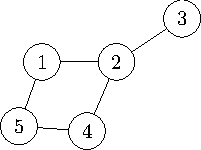
\includegraphics[width=0.4\textwidth]{chapters/gcol/figs/examplegraph1-figure2.pdf}
    \caption{Example undirected graph with at least one possible three-colouring solution (in fact, this graph is also potentially 2-colourable, and our \gls{cps} solution might select such a solution).}
    \label{fig:gcol:examplegraph}
\end{figure}

\begin{figure}
    \centering
    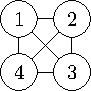
\includegraphics[width=0.2\textwidth]{chapters/gcol/figs/examplegraph1-figure3.pdf}
    \caption{Example undirected graph with no valid 3-colouring solutions.}
    \label{fig:gcol:examplegraphnosol}
\end{figure}

\subsection{Successful example}
For the graph in \autoref{fig:gcol:examplegraph}, we begin with a single top-level cell situated in the environment and in state \(s_0\).  From the hypothetical set of nodes \(V = \{1, 2, 3, 4, 5\}\) we derive the functor \(V' = \cpfunc{v}{\cpfunc{n}{1}~\cpfunc{n}{2}~\cpfunc{n}{3}~\cpfunc{n}{4}~\cpfunc{n}{5}}\), and the set of objects \[ 
E' = \{\cpfunc{e}{\cpfunc{n}{1} \, \cpfunc{n}{2}},~\cpfunc{e}{\cpfunc{n}{1} \, \cpfunc{n}{5}},~\cpfunc{e}{\cpfunc{n}{2} \, \cpfunc{n}{3}},~\cpfunc{e}{\cpfunc{n}{2} \, \cpfunc{n}{4}},~\cpfunc{e}{\cpfunc{n}{4} \, \cpfunc{n}{5}}\}
,\] representing the edges of the graph, as well as the set of colour objects \(K' = \{\cpfunc{k}{r},~\cpfunc{k}{g},~\cpfunc{k}{b}\}\), in this case representing the colours red, green and blue.  These sets of objects are all immediately within the top-level cell, along with \(\cpfunc{s}{1}\) to select node 1 at the beginning of the process, as shown in \autoref{objs:gcol:obj1}.

This beginning state, with the exception of the choice of node label inside the \(s\) object, is mandatory, but all following discussion in this subsection is merely one possible execution, due to the non-deterministic selection of colours that occurs during application of rule 1 and rule 2.

% \begin{figure}
% \begin{framed}
% \[
% e(\cpfunc{n}{1}\,\cpfunc{n}{2}) \quad \cpfunc{e}{\cpfunc{n}{1}\,\cpfunc{n}{5}} \quad \cpfunc{e}{\cpfunc{n}{2}\,\cpfunc{n}{3}} \quad \cpfunc{e}{\cpfunc{n}{2}\,\cpfunc{n}{4}} \quad \cpfunc{e}{\cpfunc{n}{4}\,\cpfunc{n}{5}}
% \]
% \[
% \cpfunc{k}{r} \quad \cpfunc{k}{g} \quad \cpfunc{k}{b} \quad \cpfunc{s}{1}\\
% \]
% \[
% \cpfunc{v}{\cpfunc{n}{1}~\cpfunc{n}{2}~\cpfunc{n}{3}~\cpfunc{n}{4}~\cpfunc{n}{5}}
% \]
% \end{framed}
% \caption{\label{fig:gcol:obj1}Initial set of objects inside the top-level cell for \autoref{fig:gcol:examplegraph}.}
% \end{figure}

\begin{cpobjectsfloat}
\begin{cpobjects}
\cpobjectsline{\cpfunc{e}{\cpfunc{n}{1} \, \cpfunc{n}{2}} \; \cpfunc{e}{\cpfunc{n}{1} \, \cpfunc{n}{5}} \; \cpfunc{e}{\cpfunc{n}{2} \, \cpfunc{n}{3}} \; \cpfunc{e}{\cpfunc{n}{2} \, \cpfunc{n}{4}} \; \cpfunc{e}{\cpfunc{n}{4} \, \cpfunc{n}{5}} \;}
% \[
% \cpfunc{e}{\cpfunc{n}{1}\,\cpfunc{n}{2}} \quad \cpfunc{e}{\cpfunc{n}{1}\,\cpfunc{n}{5}} \quad \cpfunc{e}{\cpfunc{n}{2}\,\cpfunc{n}{3}} \quad \cpfunc{e}{\cpfunc{n}{2}\,\cpfunc{n}{4}} \quad \cpfunc{e}{\cpfunc{n}{4}\,\cpfunc{n}{5}}
% \]
\cpobjectsline{ \cpfunc{k}{r} \; \cpfunc{k}{g} \; \cpfunc{k}{b} \quad \cpfunc{s}{1} \quad \cpfunc{v}{\cpfunc{n}{1} \; \cpfunc{n}{2} \; \cpfunc{n}{3} \; \cpfunc{n}{4} \; \cpfunc{n}{5}}}
% \[
% \cpfunc{k}{r} \quad \cpfunc{k}{g} \quad \cpfunc{k}{b} \quad \cpfunc{s}{1}\\
% \]
% \[
% \cpfunc{v}{\cpfunc{n}{1}~\cpfunc{n}{2}~\cpfunc{n}{3}~\cpfunc{n}{4}~\cpfunc{n}{5}}
% \]
\end{cpobjects}
\caption{\label{objs:gcol:obj1}Initial set of objects inside the top-level cell for \autoref{fig:gcol:examplegraph}.}
\end{cpobjectsfloat}

From this starting state, rule 1 is applied, choosing node 1 to start the process with, and selecting red as its colouring.  This creates the standard \(b\) and \(l\) objects.  No other rules are applicable at this point, as the top-level cell started in state \(s_0\).  The application of this rule leaves the top-level cell in state \(s_1\).  Rule 1 will henceforth be inapplicable, as the rules provide no way to revert to state \(s_0\).

% At the next step, rule 2 is checked but found inapplicable, as at this point the \(v\) object inside the only \(b\) object will not be empty, instead containing \(\cpfunc{v}{\cpfunc{n}{2}~ \cpfunc{n}{3}~ \cpfunc{n}{4}~ \cpfunc{n}{5}}\).  Rule 3, conversely, is applicable and thus can generate further new \(b\) objects.  In this instance, two edges exist from node 1 to other nodes (2 and 5 specifically), meaning that both choices can apply, generating new \(b\) objects containing all legal  colourings.  Both nodes are chosen to connect to, but there are only two other possible colourings to choose here, as red is currently blocked due to it being selected for the first \(b\) object.  This leads to the creation of four new \(b\) objects \(b\big(\cpfunc{l}{2}~\cpfunc{m}{\cpfunc{n}{1}\,\cpfunc{c}{r}}\allowbreak ~\cpfunc{m}{\cpfunc{n}{2}\,\cpfunc{c}{g}}\allowbreak ~\cpfunc{v}{\cpfunc{n}{3}~ \cpfunc{n}{4}~ \cpfunc{n}{5}}\big)\), \(b\big(\cpfunc{l}{2}~\cpfunc{m}{\cpfunc{n}{1}\,\cpfunc{c}{r}}\allowbreak ~\cpfunc{m}{\cpfunc{n}{5}\,\cpfunc{c}{b}}\allowbreak ~\cpfunc{v}{\cpfunc{n}{2}~ \cpfunc{n}{3}~ \cpfunc{n}{4}}\big)\) etc.

At the next step, rule 2 is checked but found inapplicable, as at this point the \(v\) object inside the only \(b\) object will not be empty, instead containing \(\cpfunc{v}{\cpfunc{n}{2}~ \cpfunc{n}{3}~ \cpfunc{n}{4}~ \cpfunc{n}{5}}\).  Rule 3, conversely, is applicable and thus can generate further new \(b\) objects.  In this instance, two edges exist from node 1 to other nodes (2 and 5 specifically), meaning that both choices can apply, generating new \(b\) objects containing all legal  colourings.  Both nodes are chosen to connect to, but there are only two other possible colourings to choose here, as red is currently blocked due to it being selected for the first \(b\) object.  This leads to the creation of four new \(b\) objects \(\cpfunc{b}{\cpfunc{l}{2}~\cpfunc{m}{\cpfunc{n}{1} \, \cpfunc{c}{r}}\allowbreak ~\cpfunc{m}{\cpfunc{n}{2} \, \cpfunc{c}{g}}\allowbreak ~\cpfunc{v}{\cpfunc{n}{3}~ \cpfunc{n}{4}~ \cpfunc{n}{5}}}\), \(\cpfunc{b}{\cpfunc{l}{2}~\cpfunc{m}{\cpfunc{n}{1} \, \cpfunc{c}{r}}\allowbreak ~\cpfunc{m}{\cpfunc{n}{5} \, \cpfunc{c}{b}}\allowbreak ~\cpfunc{v}{\cpfunc{n}{2}~ \cpfunc{n}{3}~ \cpfunc{n}{4}}}\) etc.

Simultaneously, rule 4 is applied to sweep away the pre-existing initial \(b\) object.  Rule 5 is not applicable because a state transition to state \(s_1\) has already been selected by application of rules 3 and 4, and thus a transition to state \(s_3\) is invalid.  Finally, rule 6 is also applied to remove the old \(l\) object and introduce a newly incremented one.  \autoref{objs:gcol:obj2} lists the objects in the top-level cell at the end of this step.

% \begin{figure}
% \begin{framed}
% \[
% e(\cpfunc{n}{1}\,\cpfunc{n}{2}) \quad \cpfunc{e}{\cpfunc{n}{1}\,\cpfunc{n}{5}} \quad \cpfunc{e}{\cpfunc{n}{2}\,\cpfunc{n}{3}} \quad \cpfunc{e}{\cpfunc{n}{2}\,\cpfunc{n}{4}} \quad \cpfunc{e}{\cpfunc{n}{4}\,\cpfunc{n}{5}}
% \]
% \[
%     \cpfunc{k}{r} \quad \cpfunc{k}{g} \quad \cpfunc{k}{b} \quad \cpfunc{l}{2}
% \]
% \[
% \cpfunc{b}{\cpfunc{l}{2}~\cpfunc{m}{\cpfunc{n}{1}\,\cpfunc{c}{r}}~\cpfunc{m}{\cpfunc{n}{2}\,\cpfunc{c}{g}}~\cpfunc{v}{\cpfunc{n}{3}~ \cpfunc{n}{4}~ \cpfunc{n}{5}}}
% \]
% \[
% \cpfunc{b}{\cpfunc{l}{2}~\cpfunc{m}{\cpfunc{n}{1}\,\cpfunc{c}{r}}~\cpfunc{m}{\cpfunc{n}{2}\,\cpfunc{c}{b}}~\cpfunc{v}{\cpfunc{n}{3}~ \cpfunc{n}{4}~ \cpfunc{n}{5}}}
% \]
% \[
% \cpfunc{b}{\cpfunc{l}{2}~\cpfunc{m}{\cpfunc{n}{1}\,\cpfunc{c}{r}}~\cpfunc{m}{\cpfunc{n}{5}\,\cpfunc{c}{g}}~\cpfunc{v}{\cpfunc{n}{2}~ \cpfunc{n}{3}~ \cpfunc{n}{4}}}
% \]
% \[
% \cpfunc{b}{\cpfunc{l}{2}~\cpfunc{m}{\cpfunc{n}{1}\,\cpfunc{c}{r}}~\cpfunc{m}{\cpfunc{n}{5}\,\cpfunc{c}{b}}~\cpfunc{v}{\cpfunc{n}{2}~ \cpfunc{n}{3}~ \cpfunc{n}{4}}}
% \]
% \end{framed}
% \caption{\label{fig:gcol:obj2}Set of objects inside the top-level cell after the second step (i.e. after one application of rules 3, 4 \& 6) for \autoref{fig:gcol:examplegraph}.}
% \end{figure}

\begin{cpobjectsfloat}
\begin{cpobjects}
\cpobjectsline{
\cpfunc{e}{\cpfunc{n}{1} \, \cpfunc{n}{2}} \; \cpfunc{e}{\cpfunc{n}{1} \, \cpfunc{n}{5}} \; \cpfunc{e}{\cpfunc{n}{2} \, \cpfunc{n}{3}} \; \cpfunc{e}{\cpfunc{n}{2} \, \cpfunc{n}{4}} \; \cpfunc{e}{\cpfunc{n}{4} \, \cpfunc{n}{5}}
}
\cpobjectsline{
    \cpfunc{k}{r} \; \cpfunc{k}{g} \; \cpfunc{k}{b} \quad \cpfunc{l}{2}
}
\cpobjectsline{
\cpfunc{b}{\cpfunc{l}{2}~\cpfunc{m}{\cpfunc{n}{1} \, \cpfunc{c}{r}}~\cpfunc{m}{\cpfunc{n}{2} \, \cpfunc{c}{g}}~\cpfunc{v}{\cpfunc{n}{3}~ \cpfunc{n}{4}~ \cpfunc{n}{5}}}
}
\cpobjectsline{
\cpfunc{b}{\cpfunc{l}{2}~\cpfunc{m}{\cpfunc{n}{1} \, \cpfunc{c}{r}}~\cpfunc{m}{\cpfunc{n}{2} \, \cpfunc{c}{b}}~\cpfunc{v}{\cpfunc{n}{3}~ \cpfunc{n}{4}~ \cpfunc{n}{5}}}
}
\cpobjectsline{
\cpfunc{b}{\cpfunc{l}{2}~\cpfunc{m}{\cpfunc{n}{1} \, \cpfunc{c}{r}}~\cpfunc{m}{\cpfunc{n}{5} \, \cpfunc{c}{g}}~\cpfunc{v}{\cpfunc{n}{2}~ \cpfunc{n}{3}~ \cpfunc{n}{4}}}
}
\cpobjectsline{
\cpfunc{b}{\cpfunc{l}{2}~\cpfunc{m}{\cpfunc{n}{1} \, \cpfunc{c}{r}}~\cpfunc{m}{\cpfunc{n}{5} \, \cpfunc{c}{b}}~\cpfunc{v}{\cpfunc{n}{2}~ \cpfunc{n}{3}~ \cpfunc{n}{4}}}
}
\end{cpobjects}
\caption{\label{objs:gcol:obj2}Set of objects inside the top-level cell after the second step (i.e. after one application of rules 3, 4 \& 6) for \autoref{fig:gcol:examplegraph}.}
\end{cpobjectsfloat}

The next step proceeds almost identically to the previous one, except that there are a greater number of new objects created (see \autoref{objs:gcol:obj3}).  At the previous step, the edges both between node 1 and node 5, and node 1 and node 2, were explored.  In this next step, edges between node 1 and node 5, node 1 and node 2 (where these edges were not explored previously for a given \(b\) object), node 5 and node 4, and node 2 and node 3 are all explored, with all objects that will not have direct colour conflicts instantiated as per rule 3.

% \begin{figure}
% \begin{framed}
% \begin{gather*}
%     \cpfunc{e}{\cpfunc{n}{1}\,\cpfunc{n}{2}} \quad \cpfunc{e}{\cpfunc{n}{1}\,\cpfunc{n}{5}} \quad \cpfunc{e}{\cpfunc{n}{2}\,\cpfunc{n}{3}} \quad \cpfunc{e}{\cpfunc{n}{2}\,\cpfunc{n}{4}} \quad \cpfunc{e}{\cpfunc{n}{4}\,\cpfunc{n}{5}}\\
%     \cpfunc{k}{r} \quad \cpfunc{k}{g} \quad \cpfunc{k}{b} \quad \cpfunc{l}{3}\\
%     \cpfunc{b}{\cpfunc{l}{3}~\cpfunc{m}{\cpfunc{n}{1}\,\cpfunc{c}{r}}~\cpfunc{m}{\cpfunc{n}{2}\,\cpfunc{c}{g}}~\cpfunc{m}{\cpfunc{n}{5}\,\cpfunc{c}{g}}~\cpfunc{v}{\cpfunc{n}{3}~ \cpfunc{n}{4}}} \\
%     \cpfunc{b}{\cpfunc{l}{3}~\cpfunc{m}{\cpfunc{n}{1}\,\cpfunc{c}{r}}~\cpfunc{m}{\cpfunc{n}{2}\,\cpfunc{c}{g}}~\cpfunc{m}{\cpfunc{n}{5}\,\cpfunc{c}{b}}~\cpfunc{v}{\cpfunc{n}{3}~ \cpfunc{n}{4}}} \\
%     \cpfunc{b}{\cpfunc{l}{3}~\cpfunc{m}{\cpfunc{n}{1}\,\cpfunc{c}{r}}~\cpfunc{m}{\cpfunc{n}{5}\,\cpfunc{c}{g}}~\cpfunc{m}{\cpfunc{n}{2}\,\cpfunc{c}{g}}~\cpfunc{v}{\cpfunc{n}{3}~ \cpfunc{n}{4}}} \\
%     \cpfunc{b}{\cpfunc{l}{3}~\cpfunc{m}{\cpfunc{n}{1}\,\cpfunc{c}{r}}~\cpfunc{m}{\cpfunc{n}{5}\,\cpfunc{c}{g}}~\cpfunc{m}{\cpfunc{n}{2}\,\cpfunc{c}{b}}~\cpfunc{v}{\cpfunc{n}{3}~ \cpfunc{n}{4}}} \\
%     \vdots\\
%     \cpfunc{b}{\cpfunc{l}{3}~\cpfunc{m}{\cpfunc{n}{1}\,\cpfunc{c}{r}}~\cpfunc{m}{\cpfunc{n}{2}\,\cpfunc{c}{b}}~\cpfunc{m}{\cpfunc{n}{3}\,\cpfunc{c}{r}}~\cpfunc{v}{\cpfunc{n}{4}~ \cpfunc{n}{5}}} \\
%     \cpfunc{b}{\cpfunc{l}{3}~\cpfunc{m}{\cpfunc{n}{1}\,\cpfunc{c}{r}}~\cpfunc{m}{\cpfunc{n}{2}\,\cpfunc{c}{b}}~\cpfunc{m}{\cpfunc{n}{3}\,\cpfunc{c}{g}}~\cpfunc{v}{\cpfunc{n}{4}~ \cpfunc{n}{5}}}
% \end{gather*}
% \end{framed}
% \caption{\label{fig:gcol:obj3}Set of objects inside the top-level cell after the third step for \autoref{fig:gcol:examplegraph}.  Note that there are some identical objects here which have been created independently.}
% \end{figure}

\begin{cpobjectsfloat}
\begin{cpobjects}
\begin{gather*}
    \cpfunc{e}{\cpfunc{n}{1} \, \cpfunc{n}{2}} \; \cpfunc{e}{\cpfunc{n}{1} \, \cpfunc{n}{5}} \; \cpfunc{e}{\cpfunc{n}{2} \, \cpfunc{n}{3}} \; \cpfunc{e}{\cpfunc{n}{2} \, \cpfunc{n}{4}} \; \cpfunc{e}{\cpfunc{n}{4} \, \cpfunc{n}{5}}\\
    \cpfunc{k}{r} \; \cpfunc{k}{g} \; \cpfunc{k}{b} \quad \cpfunc{l}{3}\\
    \cpfunc{b}{\cpfunc{l}{3}~\cpfunc{m}{\cpfunc{n}{1} \, \cpfunc{c}{r}}~\cpfunc{m}{\cpfunc{n}{2} \, \cpfunc{c}{g}}~\cpfunc{m}{\cpfunc{n}{5} \, \cpfunc{c}{g}}~\cpfunc{v}{\cpfunc{n}{3}~ \cpfunc{n}{4}}} \\
    \cpfunc{b}{\cpfunc{l}{3}~\cpfunc{m}{\cpfunc{n}{1} \, \cpfunc{c}{r}}~\cpfunc{m}{\cpfunc{n}{2} \, \cpfunc{c}{g}}~\cpfunc{m}{\cpfunc{n}{5} \, \cpfunc{c}{b}}~\cpfunc{v}{\cpfunc{n}{3}~ \cpfunc{n}{4}}} \\
    \cpfunc{b}{\cpfunc{l}{3}~\cpfunc{m}{\cpfunc{n}{1} \, \cpfunc{c}{r}}~\cpfunc{m}{\cpfunc{n}{5} \, \cpfunc{c}{g}}~\cpfunc{m}{\cpfunc{n}{2} \, \cpfunc{c}{g}}~\cpfunc{v}{\cpfunc{n}{3}~ \cpfunc{n}{4}}} \\
    \cpfunc{b}{\cpfunc{l}{3}~\cpfunc{m}{\cpfunc{n}{1} \, \cpfunc{c}{r}}~\cpfunc{m}{\cpfunc{n}{5} \, \cpfunc{c}{g}}~\cpfunc{m}{\cpfunc{n}{2} \, \cpfunc{c}{b}}~\cpfunc{v}{\cpfunc{n}{3}~ \cpfunc{n}{4}}} \\
    \vdots\\
    \cpfunc{b}{\cpfunc{l}{3}~\cpfunc{m}{\cpfunc{n}{1} \, \cpfunc{c}{r}}~\cpfunc{m}{\cpfunc{n}{2} \, \cpfunc{c}{b}}~\cpfunc{m}{\cpfunc{n}{3} \, \cpfunc{c}{r}}~\cpfunc{v}{\cpfunc{n}{4}~ \cpfunc{n}{5}}} \\
    \cpfunc{b}{\cpfunc{l}{3}~\cpfunc{m}{\cpfunc{n}{1} \, \cpfunc{c}{r}}~\cpfunc{m}{\cpfunc{n}{2} \, \cpfunc{c}{b}}~\cpfunc{m}{\cpfunc{n}{3} \, \cpfunc{c}{g}}~\cpfunc{v}{\cpfunc{n}{4}~ \cpfunc{n}{5}}}
\end{gather*}
\end{cpobjects}
\caption{\label{objs:gcol:obj3}Set of objects inside the top-level cell after the third step for \autoref{fig:gcol:examplegraph}.  Note that there are some identical objects here which have been created independently.}
\end{cpobjectsfloat}

At the fourth step, a large number of further objects are created, some of which are listed in \autoref{objs:gcol:obj4}.  The key difference between this step and the previous one is that the final inhibitor on rule 3 plays a much greater part.  At this step, many of the potential instantiations of new node and colouration selections will include conflicts between the newly-selected node and colour, and one or more of the node and colour selections made earlier.  The final inhibitor prevents instantiation of these choices, avoiding threats to correctness.  An alternative solution to the problem would be to include another following step, where those invalid instatiations are detected and removed, but the inhibitor makes this unnecessary.  

% \begin{figure}
% \begin{framed}
% \begin{gather*}
%     \cpfunc{e}{\cpfunc{n}{1}\,\cpfunc{n}{2}} \quad \cpfunc{e}{\cpfunc{n}{1}\,\cpfunc{n}{5}} \quad \cpfunc{e}{\cpfunc{n}{2}\,\cpfunc{n}{3}} \quad \cpfunc{e}{\cpfunc{n}{2}\,\cpfunc{n}{4}} \quad \cpfunc{e}{\cpfunc{n}{4}\,\cpfunc{n}{5}}\\
%     \cpfunc{k}{r} \quad \cpfunc{k}{g} \quad \cpfunc{k}{b} \quad \cpfunc{l}{4}\\
%     % \cpfunc{b}{\cpfunc{l}{3}~m(\cpfunc{n}{1}\,\cpfunc{c}{r}}~\cpfunc{m}{\cpfunc{n}{5}\,\cpfunc{c}{g}}~\cpfunc{m}{\cpfunc{n}{4}\,\cpfunc{c}{r}}~\cpfunc{v}{2~ 3}) \\
%     \cpfunc{b}{\cpfunc{l}{4}~\cpfunc{m}{\cpfunc{n}{1}\,\cpfunc{c}{r}}~\cpfunc{m}{\cpfunc{n}{5}\,\cpfunc{c}{g}}~\cpfunc{m}{\cpfunc{n}{4}\,\cpfunc{c}{r}}~\cpfunc{m}{\cpfunc{n}{2}\,\cpfunc{c}{g}}~\cpfunc{v}{\cpfunc{n}{3}}} \\
%     \cpfunc{b}{\cpfunc{l}{4}~\cpfunc{m}{\cpfunc{n}{1}\,\cpfunc{c}{r}}~\cpfunc{m}{\cpfunc{n}{5}\,\cpfunc{c}{g}}~\cpfunc{m}{\cpfunc{n}{4}\,\cpfunc{c}{r}}~\cpfunc{m}{\cpfunc{n}{2}\,\cpfunc{c}{b}}~\cpfunc{v}{\cpfunc{n}{3}}} \\
%     \cpfunc{b}{\cpfunc{l}{4}~\cpfunc{m}{\cpfunc{n}{1}\,\cpfunc{c}{r}}~\cpfunc{m}{\cpfunc{n}{5}\,\cpfunc{c}{g}}~\cpfunc{m}{\cpfunc{n}{4}\,\cpfunc{c}{r}}~\cpfunc{m}{\cpfunc{n}{2}\,\cpfunc{c}{g}}~\cpfunc{v}{\cpfunc{n}{3}}} \\
%     \cpfunc{b}{\cpfunc{l}{4}~\cpfunc{m}{\cpfunc{n}{1}\,\cpfunc{c}{r}}~\cpfunc{m}{\cpfunc{n}{5}\,\cpfunc{c}{g}}~\cpfunc{m}{\cpfunc{n}{4}\,\cpfunc{c}{r}}~\cpfunc{m}{\cpfunc{n}{2}\,\cpfunc{c}{b}}~\cpfunc{v}{\cpfunc{n}{3}}} \\
%     \vdots\\
%         \cpfunc{b}{\cpfunc{l}{4}~\cpfunc{m}{\cpfunc{n}{1}\,\cpfunc{c}{r}}~\cpfunc{m}{\cpfunc{n}{2}\,\cpfunc{c}{b}}~\cpfunc{m}{\cpfunc{n}{3}\,\cpfunc{c}{g}}~\cpfunc{m}{\cpfunc{n}{5}\,\cpfunc{c}{g}}~\cpfunc{v}{\cpfunc{n}{4}}} \\
%     \cpfunc{b}{\cpfunc{l}{4}~\cpfunc{m}{\cpfunc{n}{1}\,\cpfunc{c}{r}}~\cpfunc{m}{\cpfunc{n}{2}\,\cpfunc{c}{b}}~\cpfunc{m}{\cpfunc{n}{3}\,\cpfunc{c}{g}}~\cpfunc{m}{\cpfunc{n}{5}\,\cpfunc{c}{b}}~\cpfunc{v}{\cpfunc{n}{4}}}
% \end{gather*}
% \end{framed}
% \caption{\label{fig:gcol:obj4}Set of objects inside the top-level cell after the fourth step for \autoref{fig:gcol:examplegraph}.}
% \end{figure}  

\begin{cpobjectsfloat}
\begin{cpobjects}
\begin{gather*}
    \cpfunc{e}{\cpfunc{n}{1} \, \cpfunc{n}{2}} \; \cpfunc{e}{\cpfunc{n}{1} \, \cpfunc{n}{5}} \; \cpfunc{e}{\cpfunc{n}{2} \, \cpfunc{n}{3}} \; \cpfunc{e}{\cpfunc{n}{2} \, \cpfunc{n}{4}} \; \cpfunc{e}{\cpfunc{n}{4} \, \cpfunc{n}{5}}\\
    \cpfunc{k}{r} \; \cpfunc{k}{g} \; \cpfunc{k}{b} \quad \cpfunc{l}{4}\\
    % \cpfunc{b}{\cpfunc{l}{3}~m(\cpfunc{n}{1}\,\cpfunc{c}{r}}~\cpfunc{m}{\cpfunc{n}{5}\,\cpfunc{c}{g}}~\cpfunc{m}{\cpfunc{n}{4}\,\cpfunc{c}{r}}~\cpfunc{v}{2~ 3}) \\
    \cpfunc{b}{\cpfunc{l}{4}~\cpfunc{m}{\cpfunc{n}{1} \, \cpfunc{c}{r}}~\cpfunc{m}{\cpfunc{n}{5} \, \cpfunc{c}{g}}~\cpfunc{m}{\cpfunc{n}{4} \, \cpfunc{c}{r}}~\cpfunc{m}{\cpfunc{n}{2} \, \cpfunc{c}{g}}~\cpfunc{v}{\cpfunc{n}{3}}} \\
    \cpfunc{b}{\cpfunc{l}{4}~\cpfunc{m}{\cpfunc{n}{1} \, \cpfunc{c}{r}}~\cpfunc{m}{\cpfunc{n}{5} \, \cpfunc{c}{g}}~\cpfunc{m}{\cpfunc{n}{4} \, \cpfunc{c}{r}}~\cpfunc{m}{\cpfunc{n}{2} \, \cpfunc{c}{b}}~\cpfunc{v}{\cpfunc{n}{3}}} \\
    \cpfunc{b}{\cpfunc{l}{4}~\cpfunc{m}{\cpfunc{n}{1} \, \cpfunc{c}{r}}~\cpfunc{m}{\cpfunc{n}{5} \, \cpfunc{c}{g}}~\cpfunc{m}{\cpfunc{n}{4} \, \cpfunc{c}{r}}~\cpfunc{m}{\cpfunc{n}{2} \, \cpfunc{c}{g}}~\cpfunc{v}{\cpfunc{n}{3}}} \\
    \cpfunc{b}{\cpfunc{l}{4}~\cpfunc{m}{\cpfunc{n}{1} \, \cpfunc{c}{r}}~\cpfunc{m}{\cpfunc{n}{5} \, \cpfunc{c}{g}}~\cpfunc{m}{\cpfunc{n}{4} \, \cpfunc{c}{r}}~\cpfunc{m}{\cpfunc{n}{2} \, \cpfunc{c}{b}}~\cpfunc{v}{\cpfunc{n}{3}}} \\
    \vdots\\
        \cpfunc{b}{\cpfunc{l}{4}~\cpfunc{m}{\cpfunc{n}{1} \, \cpfunc{c}{r}}~\cpfunc{m}{\cpfunc{n}{2} \, \cpfunc{c}{b}}~\cpfunc{m}{\cpfunc{n}{3} \, \cpfunc{c}{g}}~\cpfunc{m}{\cpfunc{n}{5} \, \cpfunc{c}{g}}~\cpfunc{v}{\cpfunc{n}{4}}} \\
    \cpfunc{b}{\cpfunc{l}{4}~\cpfunc{m}{\cpfunc{n}{1} \, \cpfunc{c}{r}}~\cpfunc{m}{\cpfunc{n}{2} \, \cpfunc{c}{b}}~\cpfunc{m}{\cpfunc{n}{3} \, \cpfunc{c}{g}}~\cpfunc{m}{\cpfunc{n}{5} \, \cpfunc{c}{b}}~\cpfunc{v}{\cpfunc{n}{4}}}
\end{gather*}

\end{cpobjects}
\caption{\label{objs:gcol:obj4}Set of objects inside the top-level cell after the fourth step for \autoref{fig:gcol:examplegraph}.}
\end{cpobjectsfloat}

Step 5 proceeds analogously.  At the end of step 5 a number of \(b\) objects which contain valid colourings of the whole graph will be present inside the top-level cell.  At the sixth step, rule 2 will detect this by the fact that said objects will contain empty \(v\) functors.  For example, \autoref{objs:gcol:obj6} shows some of the potential solutions that could be generated, reflecting the state of the system at the end of the fifth step.  In fact, the first potential solution shows that in this case it is possible to completely and validly colour this graph using only two colours.  This solution may or may not be chosen when rule 2 is applied.  At the end of the sixth step, rule 2 will select one of the possible solutions and emit it to the environment.  The top-level cell will also transition to state \(s_2\), signalling that the process succeeded.

% \begin{figure}
% \begin{framed}
% \begin{gather*}
%     \cpfunc{e}{\cpfunc{n}{1}\,\cpfunc{n}{2}} \quad \cpfunc{e}{\cpfunc{n}{1}\,\cpfunc{n}{5}} \quad \cpfunc{e}{\cpfunc{n}{2}\,\cpfunc{n}{3}} \quad \cpfunc{e}{\cpfunc{n}{2}\,\cpfunc{n}{4}} \quad \cpfunc{e}{\cpfunc{n}{4}\,\cpfunc{n}{5}}\\
%     \cpfunc{k}{r} \quad \cpfunc{k}{g} \quad \cpfunc{k}{b} \quad \cpfunc{l}{5}\\
%     \cpfunc{b}{\cpfunc{l}{5}~\cpfunc{m}{\cpfunc{n}{1}\,\cpfunc{c}{r}}~\cpfunc{m}{\cpfunc{n}{5}\,\cpfunc{c}{g}}~\cpfunc{m}{\cpfunc{n}{4}\,\cpfunc{c}{r}}~\cpfunc{m}{\cpfunc{n}{2}\,\cpfunc{c}{g}}~\cpfunc{m}{\cpfunc{n}{3}\,\cpfunc{c}{r}}~v()} \\
%     \cpfunc{b}{\cpfunc{l}{5}~\cpfunc{m}{\cpfunc{n}{1}\,\cpfunc{c}{r}}~\cpfunc{m}{\cpfunc{n}{5}\,\cpfunc{c}{g}}~\cpfunc{m}{\cpfunc{n}{4}\,\cpfunc{c}{r}}~\cpfunc{m}{\cpfunc{n}{2}\,\cpfunc{c}{g}}~\cpfunc{m}{\cpfunc{n}{3}\,\cpfunc{c}{b}}~v()} \\
%             \vdots\\
%     \cpfunc{b}{\cpfunc{l}{5}~\cpfunc{m}{\cpfunc{n}{1}\,\cpfunc{c}{r}}~\cpfunc{m}{\cpfunc{n}{2}\,\cpfunc{c}{b}}~\cpfunc{m}{\cpfunc{n}{3}\,\cpfunc{c}{g}}~\cpfunc{m}{\cpfunc{n}{5}\,\cpfunc{c}{g}}~\cpfunc{m}{\cpfunc{n}{4}\,\cpfunc{c}{r}}~v()} \\
%     \cpfunc{b}{\cpfunc{l}{5}~\cpfunc{m}{\cpfunc{n}{1}\,\cpfunc{c}{r}}~\cpfunc{m}{\cpfunc{n}{2}\,\cpfunc{c}{b}}~\cpfunc{m}{\cpfunc{n}{3}\,\cpfunc{c}{g}}~\cpfunc{m}{\cpfunc{n}{5}\,\cpfunc{c}{g}}~\cpfunc{m}{\cpfunc{n}{4}\,\cpfunc{c}{r}}~v()}
% \end{gather*}
% \end{framed}
% \caption{\label{fig:obj6}Set of objects inside the top-level cell after the fifth step for \autoref{fig:gcol:examplegraph}.}
% \end{figure}

\begin{cpobjectsfloat}
\begin{cpobjects}

\begin{gather*}
    \cpfunc{e}{\cpfunc{n}{1} \, \cpfunc{n}{2}} \; \cpfunc{e}{\cpfunc{n}{1} \, \cpfunc{n}{5}} \; \cpfunc{e}{\cpfunc{n}{2} \, \cpfunc{n}{3}} \; \cpfunc{e}{\cpfunc{n}{2} \, \cpfunc{n}{4}} \; \cpfunc{e}{\cpfunc{n}{4} \, \cpfunc{n}{5}}\\
    \cpfunc{k}{r} \; \cpfunc{k}{g} \; \cpfunc{k}{b} \quad \cpfunc{l}{5}\\
    \cpfunc{b}{\cpfunc{l}{5}~\cpfunc{m}{\cpfunc{n}{1} \, \cpfunc{c}{r}}~\cpfunc{m}{\cpfunc{n}{5} \, \cpfunc{c}{g}}~\cpfunc{m}{\cpfunc{n}{4} \, \cpfunc{c}{r}}~\cpfunc{m}{\cpfunc{n}{2} \, \cpfunc{c}{g}}~\cpfunc{m}{\cpfunc{n}{3} \, \cpfunc{c}{r}}~v()} \\
    \cpfunc{b}{\cpfunc{l}{5}~\cpfunc{m}{\cpfunc{n}{1} \, \cpfunc{c}{r}}~\cpfunc{m}{\cpfunc{n}{5} \, \cpfunc{c}{g}}~\cpfunc{m}{\cpfunc{n}{4} \, \cpfunc{c}{r}}~\cpfunc{m}{\cpfunc{n}{2} \, \cpfunc{c}{g}}~\cpfunc{m}{\cpfunc{n}{3} \, \cpfunc{c}{b}}~v()} \\
            \vdots\\
    \cpfunc{b}{\cpfunc{l}{5}~\cpfunc{m}{\cpfunc{n}{1} \, \cpfunc{c}{r}}~\cpfunc{m}{\cpfunc{n}{2} \, \cpfunc{c}{b}}~\cpfunc{m}{\cpfunc{n}{3} \, \cpfunc{c}{g}}~\cpfunc{m}{\cpfunc{n}{5} \, \cpfunc{c}{g}}~\cpfunc{m}{\cpfunc{n}{4} \, \cpfunc{c}{r}}~v()} \\
    \cpfunc{b}{\cpfunc{l}{5}~\cpfunc{m}{\cpfunc{n}{1} \, \cpfunc{c}{r}}~\cpfunc{m}{\cpfunc{n}{2} \, \cpfunc{c}{b}}~\cpfunc{m}{\cpfunc{n}{3} \, \cpfunc{c}{g}}~\cpfunc{m}{\cpfunc{n}{5} \, \cpfunc{c}{g}}~\cpfunc{m}{\cpfunc{n}{4} \, \cpfunc{c}{r}}~v()}
\end{gather*}
\end{cpobjects}
\caption{\label{objs:gcol:obj6}Set of objects inside the top-level cell after the fifth step for \autoref{fig:gcol:examplegraph}.}
\end{cpobjectsfloat}

% ------------------------------------------------

\subsection{Failure example}
Here we step through the execution of the algorithm when there is no possible valid 3-colouring solution, using the graph depicted in \autoref{fig:gcol:examplegraphnosol}.  The system begins with the objects depicted in \autoref{objs:gcol:objn1}.

% \begin{figure}
% \begin{framed}
% \begin{gather*}
%     \cpfunc{e}{\cpfunc{n}{1}\,\cpfunc{n}{2}} \quad \cpfunc{e}{\cpfunc{n}{1}\,\cpfunc{n}{3}} \quad \cpfunc{e}{\cpfunc{n}{1}\,\cpfunc{n}{4}} \quad \cpfunc{e}{\cpfunc{n}{2}\,\cpfunc{n}{3}} \quad \cpfunc{e}{\cpfunc{n}{2}\,\cpfunc{n}{4}} \quad \cpfunc{e}{\cpfunc{n}{3}\,\cpfunc{n}{4}}\\
%     \cpfunc{k}{r} \quad \cpfunc{k}{g} \quad \cpfunc{k}{b} \quad \cpfunc{s}{1}\\
%     \cpfunc{v}{\cpfunc{n}{1}~\cpfunc{n}{2}~\cpfunc{n}{3}~\cpfunc{n}{4}}
% \end{gather*}
% \end{framed}
% \caption{\label{fig:objn1}Initial set of objects inside the top-level cell for \autoref{fig:gcol:examplegraphnosol}.}
% \end{figure}

\begin{cpobjectsfloat}
\begin{cpobjects}

\begin{gather*}
    \cpfunc{e}{\cpfunc{n}{1} \, \cpfunc{n}{2}} \; \cpfunc{e}{\cpfunc{n}{1} \, \cpfunc{n}{3}} \; \cpfunc{e}{\cpfunc{n}{1} \, \cpfunc{n}{4}} \; \cpfunc{e}{\cpfunc{n}{2} \, \cpfunc{n}{3}} \; \cpfunc{e}{\cpfunc{n}{2} \, \cpfunc{n}{4}} \; \cpfunc{e}{\cpfunc{n}{3} \, \cpfunc{n}{4}}\\
    \cpfunc{k}{r} \; \cpfunc{k}{g} \; \cpfunc{k}{b} \quad \cpfunc{s}{1}\\
    \cpfunc{v}{\cpfunc{n}{1}~\cpfunc{n}{2}~\cpfunc{n}{3}~\cpfunc{n}{4}}
\end{gather*}
\end{cpobjects}
\caption{\label{objs:gcol:objn1}Initial set of objects inside the top-level cell for \autoref{fig:gcol:examplegraphnosol}.}
\end{cpobjectsfloat}

After the first step, the application of rule 1, the objects shown in \autoref{objs:gcol:objn2} are inside the top-level cell.  This is not substantively different from the successful example above.  Likewise with the objects present in the cell at the end of the second step, shown in \autoref{objs:gcol:objn3}.

% \begin{figure}
% \begin{framed}
% \begin{gather*}
%     \cpfunc{e}{\cpfunc{n}{1}\,\cpfunc{n}{2}} \quad \cpfunc{e}{\cpfunc{n}{1}\,\cpfunc{n}{3}} \quad \cpfunc{e}{\cpfunc{n}{1}\,\cpfunc{n}{4}} \quad \cpfunc{e}{\cpfunc{n}{2}\,\cpfunc{n}{3}} \quad \cpfunc{e}{\cpfunc{n}{2}\,\cpfunc{n}{4}} \quad \cpfunc{e}{\cpfunc{n}{3}\,\cpfunc{n}{4}}\\
%     \cpfunc{k}{r} \quad \cpfunc{k}{g} \quad \cpfunc{k}{b} \quad \cpfunc{l}{1}\\
%     \cpfunc{b}{\cpfunc{l}{1}~\cpfunc{m}{\cpfunc{n}{1}\,\cpfunc{c}{r}}~\cpfunc{v}{\cpfunc{n}{2}~\cpfunc{n}{3}~\cpfunc{n}{4}}}
% \end{gather*}
% \end{framed}
% \caption{\label{fig:objn2}Set of objects inside the top-level cell at the end of step 1, for \autoref{fig:gcol:examplegraphnosol}.}
% \end{figure}

\begin{cpobjectsfloat}
\begin{cpobjects}

\begin{gather*}
    \cpfunc{e}{\cpfunc{n}{1} \, \cpfunc{n}{2}} \; \cpfunc{e}{\cpfunc{n}{1} \, \cpfunc{n}{3}} \; \cpfunc{e}{\cpfunc{n}{1} \, \cpfunc{n}{4}} \; \cpfunc{e}{\cpfunc{n}{2} \, \cpfunc{n}{3}} \; \cpfunc{e}{\cpfunc{n}{2} \, \cpfunc{n}{4}} \; \cpfunc{e}{\cpfunc{n}{3} \, \cpfunc{n}{4}}\\
    \cpfunc{k}{r} \; \cpfunc{k}{g} \; \cpfunc{k}{b} \quad \cpfunc{l}{1}\\
    \cpfunc{b}{\cpfunc{l}{1}~\cpfunc{m}{\cpfunc{n}{1} \, \cpfunc{c}{r}}~\cpfunc{v}{\cpfunc{n}{2}~\cpfunc{n}{3}~\cpfunc{n}{4}}}
\end{gather*}
\end{cpobjects}
\caption{\label{objs:gcol:objn2}Set of objects inside the top-level cell at the end of step 1, for \autoref{fig:gcol:examplegraphnosol}.}
\end{cpobjectsfloat}

% \begin{figure}
% \begin{framed}
% \begin{gather*}
%     \cpfunc{e}{\cpfunc{n}{1}\,\cpfunc{n}{2}} \quad \cpfunc{e}{\cpfunc{n}{1}\,\cpfunc{n}{3}} \quad \cpfunc{e}{\cpfunc{n}{1}\,\cpfunc{n}{4}} \quad \cpfunc{e}{\cpfunc{n}{2}\,\cpfunc{n}{3}} \quad \cpfunc{e}{\cpfunc{n}{2}\,\cpfunc{n}{4}} \quad \cpfunc{e}{\cpfunc{n}{3}\,\cpfunc{n}{4}}\\
%     \cpfunc{k}{r} \quad \cpfunc{k}{g} \quad \cpfunc{k}{b} \quad \cpfunc{l}{2}\\
%     \cpfunc{b}{\cpfunc{l}{2}~\cpfunc{m}{\cpfunc{n}{1}\,\cpfunc{c}{r}}~\cpfunc{m}{\cpfunc{n}{2}\,\cpfunc{c}{g}}~\cpfunc{v}{\cpfunc{n}{3}~\cpfunc{n}{4}}}\\
%     \cpfunc{b}{\cpfunc{l}{2}~\cpfunc{m}{\cpfunc{n}{1}\,\cpfunc{c}{r}}~\cpfunc{m}{\cpfunc{n}{2}\,\cpfunc{c}{b}}~\cpfunc{v}{\cpfunc{n}{3}~\cpfunc{n}{4}}}\\
%     \cpfunc{b}{\cpfunc{l}{2}~\cpfunc{m}{\cpfunc{n}{1}\,\cpfunc{c}{r}}~\cpfunc{m}{\cpfunc{n}{3}\,\cpfunc{c}{g}}~\cpfunc{v}{\cpfunc{n}{2}~\cpfunc{n}{4}}}\\
%     \cpfunc{b}{\cpfunc{l}{2}~\cpfunc{m}{\cpfunc{n}{1}\,\cpfunc{c}{r}}~\cpfunc{m}{\cpfunc{n}{3}\,\cpfunc{c}{b}}~\cpfunc{v}{\cpfunc{n}{2}~\cpfunc{n}{4}}}\\
%     \cpfunc{b}{\cpfunc{l}{2}~\cpfunc{m}{\cpfunc{n}{1}\,\cpfunc{c}{r}}~\cpfunc{m}{\cpfunc{n}{4}\,\cpfunc{c}{g}}~\cpfunc{v}{\cpfunc{n}{2}~\cpfunc{n}{3}}}\\
%     \cpfunc{b}{\cpfunc{l}{2}~\cpfunc{m}{\cpfunc{n}{1}\,\cpfunc{c}{r}}~\cpfunc{m}{\cpfunc{n}{4}\,\cpfunc{c}{b}}~\cpfunc{v}{\cpfunc{n}{2}~\cpfunc{n}{3}}}
% \end{gather*}
% \end{framed}
% \caption{\label{fig:objn3}Set of objects inside the top-level cell at the end of step 2, for \autoref{fig:gcol:examplegraphnosol}.}
% \end{figure}

\begin{cpobjectsfloat}
\begin{cpobjects}
\begin{gather*}
    \cpfunc{e}{\cpfunc{n}{1} \, \cpfunc{n}{2}} \; \cpfunc{e}{\cpfunc{n}{1} \, \cpfunc{n}{3}} \; \cpfunc{e}{\cpfunc{n}{1} \, \cpfunc{n}{4}} \; \cpfunc{e}{\cpfunc{n}{2} \, \cpfunc{n}{3}} \; \cpfunc{e}{\cpfunc{n}{2} \, \cpfunc{n}{4}} \; \cpfunc{e}{\cpfunc{n}{3} \, \cpfunc{n}{4}}\\
    \cpfunc{k}{r} \; \cpfunc{k}{g} \; \cpfunc{k}{b} \quad \cpfunc{l}{2}\\
    \cpfunc{b}{\cpfunc{l}{2}~\cpfunc{m}{\cpfunc{n}{1} \, \cpfunc{c}{r}}~\cpfunc{m}{\cpfunc{n}{2} \, \cpfunc{c}{g}}~\cpfunc{v}{\cpfunc{n}{3}~\cpfunc{n}{4}}}\\
    \cpfunc{b}{\cpfunc{l}{2}~\cpfunc{m}{\cpfunc{n}{1} \, \cpfunc{c}{r}}~\cpfunc{m}{\cpfunc{n}{2} \, \cpfunc{c}{b}}~\cpfunc{v}{\cpfunc{n}{3}~\cpfunc{n}{4}}}\\
    \cpfunc{b}{\cpfunc{l}{2}~\cpfunc{m}{\cpfunc{n}{1} \, \cpfunc{c}{r}}~\cpfunc{m}{\cpfunc{n}{3} \, \cpfunc{c}{g}}~\cpfunc{v}{\cpfunc{n}{2}~\cpfunc{n}{4}}}\\
    \cpfunc{b}{\cpfunc{l}{2}~\cpfunc{m}{\cpfunc{n}{1} \, \cpfunc{c}{r}}~\cpfunc{m}{\cpfunc{n}{3} \, \cpfunc{c}{b}}~\cpfunc{v}{\cpfunc{n}{2}~\cpfunc{n}{4}}}\\
    \cpfunc{b}{\cpfunc{l}{2}~\cpfunc{m}{\cpfunc{n}{1} \, \cpfunc{c}{r}}~\cpfunc{m}{\cpfunc{n}{4} \, \cpfunc{c}{g}}~\cpfunc{v}{\cpfunc{n}{2}~\cpfunc{n}{3}}}\\
    \cpfunc{b}{\cpfunc{l}{2}~\cpfunc{m}{\cpfunc{n}{1} \, \cpfunc{c}{r}}~\cpfunc{m}{\cpfunc{n}{4} \, \cpfunc{c}{b}}~\cpfunc{v}{\cpfunc{n}{2}~\cpfunc{n}{3}}}
\end{gather*}

\end{cpobjects}
\caption{\label{objs:gcol:objn3}Set of objects inside the top-level cell at the end of step 2, for \autoref{fig:gcol:examplegraphnosol}.}
\end{cpobjectsfloat}

\autoref{objs:gcol:objn4} shows the objects in the top-level cell at the end of step three.  This proceeds in much the same fashion as the previous step, but fully half of the potential instantiations from rule 3 are avoided by the rule's final inhibitor, due to inevitable colouration conflicts.

% \begin{figure}
% \begin{framed}
% \begin{gather*}
%     \cpfunc{e}{\cpfunc{n}{1}\,\cpfunc{n}{2}} \quad \cpfunc{e}{\cpfunc{n}{1}\,\cpfunc{n}{3}} \quad \cpfunc{e}{\cpfunc{n}{1}\,\cpfunc{n}{4}} \quad \cpfunc{e}{\cpfunc{n}{2}\,\cpfunc{n}{3}} \quad \cpfunc{e}{\cpfunc{n}{2}\,\cpfunc{n}{4}} \quad \cpfunc{e}{\cpfunc{n}{3}\,\cpfunc{n}{4}}\\
%     \cpfunc{k}{r} \quad \cpfunc{k}{g} \quad \cpfunc{k}{b} \quad \cpfunc{l}{3}\\
%     % \cpfunc{b}{\cpfunc{l}{2}~m(\cpfunc{n}{1}\,\cpfunc{c}{r}}~\cpfunc{m}{\cpfunc{n}{2}\,\cpfunc{c}{g}}~\cpfunc{v}{\cpfunc{n}{3}~\cpfunc{n}{4}})\\
%     \cpfunc{b}{\cpfunc{l}{3}~\cpfunc{m}{\cpfunc{n}{1}\,\cpfunc{c}{r}}~\cpfunc{m}{\cpfunc{n}{2}\,\cpfunc{c}{g}}~\cpfunc{m}{\cpfunc{n}{3}\,\cpfunc{c}{b}}~\cpfunc{v}{\cpfunc{n}{4}}}\\
%     \cpfunc{b}{\cpfunc{l}{3}~\cpfunc{m}{\cpfunc{n}{1}\,\cpfunc{c}{r}}~\cpfunc{m}{\cpfunc{n}{2}\,\cpfunc{c}{g}}~\cpfunc{m}{\cpfunc{n}{3}\,\cpfunc{c}{b}}~\cpfunc{v}{\cpfunc{n}{4}}}\\
%         \vdots\\
%     \cpfunc{b}{\cpfunc{l}{3}~\cpfunc{m}{\cpfunc{n}{1}\,\cpfunc{c}{r}}~\cpfunc{m}{\cpfunc{n}{2}\,\cpfunc{c}{g}}~\cpfunc{m}{\cpfunc{n}{4}\,\cpfunc{c}{b}}~\cpfunc{v}{\cpfunc{n}{3}}}\\
%     \cpfunc{b}{\cpfunc{l}{3}~\cpfunc{m}{\cpfunc{n}{1}\,\cpfunc{c}{r}}~\cpfunc{m}{\cpfunc{n}{2}\,\cpfunc{c}{g}}~\cpfunc{m}{\cpfunc{n}{4}\,\cpfunc{c}{b}}~\cpfunc{v}{\cpfunc{n}{3}}}
% \end{gather*}
% \end{framed}
% \caption{\label{fig:objn4}Set of objects inside the top-level cell at the end of step 3, for \autoref{fig:gcol:examplegraphnosol}.}
% \end{figure}

\begin{cpobjectsfloat}
\begin{cpobjects}

\begin{gather*}
    \cpfunc{e}{\cpfunc{n}{1} \, \cpfunc{n}{2}} \; \cpfunc{e}{\cpfunc{n}{1} \, \cpfunc{n}{3}} \; \cpfunc{e}{\cpfunc{n}{1} \, \cpfunc{n}{4}} \; \cpfunc{e}{\cpfunc{n}{2} \, \cpfunc{n}{3}} \; \cpfunc{e}{\cpfunc{n}{2} \, \cpfunc{n}{4}} \; \cpfunc{e}{\cpfunc{n}{3} \, \cpfunc{n}{4}}\\
    \cpfunc{k}{r} \; \cpfunc{k}{g} \; \cpfunc{k}{b} \quad \cpfunc{l}{3}\\
    % \cpfunc{b}{\cpfunc{l}{2}~m(\cpfunc{n}{1}\,\cpfunc{c}{r}}~\cpfunc{m}{\cpfunc{n}{2}\,\cpfunc{c}{g}}~\cpfunc{v}{\cpfunc{n}{3}~\cpfunc{n}{4}})\\
    \cpfunc{b}{\cpfunc{l}{3}~\cpfunc{m}{\cpfunc{n}{1} \, \cpfunc{c}{r}}~\cpfunc{m}{\cpfunc{n}{2} \, \cpfunc{c}{g}}~\cpfunc{m}{\cpfunc{n}{3} \, \cpfunc{c}{b}}~\cpfunc{v}{\cpfunc{n}{4}}}\\
    \cpfunc{b}{\cpfunc{l}{3}~\cpfunc{m}{\cpfunc{n}{1} \, \cpfunc{c}{r}}~\cpfunc{m}{\cpfunc{n}{2} \, \cpfunc{c}{g}}~\cpfunc{m}{\cpfunc{n}{3} \, \cpfunc{c}{b}}~\cpfunc{v}{\cpfunc{n}{4}}}\\
        \vdots\\
    \cpfunc{b}{\cpfunc{l}{3}~\cpfunc{m}{\cpfunc{n}{1} \, \cpfunc{c}{r}}~\cpfunc{m}{\cpfunc{n}{2} \, \cpfunc{c}{g}}~\cpfunc{m}{\cpfunc{n}{4} \, \cpfunc{c}{b}}~\cpfunc{v}{\cpfunc{n}{3}}}\\
    \cpfunc{b}{\cpfunc{l}{3}~\cpfunc{m}{\cpfunc{n}{1} \, \cpfunc{c}{r}}~\cpfunc{m}{\cpfunc{n}{2} \, \cpfunc{c}{g}}~\cpfunc{m}{\cpfunc{n}{4} \, \cpfunc{c}{b}}~\cpfunc{v}{\cpfunc{n}{3}}}
\end{gather*}
\end{cpobjects}
\caption{\label{objs:gcol:objn4}Set of objects inside the top-level cell at the end of step 3, for \autoref{fig:gcol:examplegraphnosol}.}
\end{cpobjectsfloat}

Finally, \autoref{objs:gcol:objn5} shows the objects in the top-level cell as at the end of step 4.  Due to the fully-connected nature of the graph in \autoref{fig:gcol:examplegraphnosol}, every possible solution will contain at least one instance of proposed contiguous colouration, thus making every possible solution invalid.  This means that rule 3 will not create any new \(b\) objects, while rule 4 will remove the pre-existing ones.

% \begin{figure}
% \begin{framed}
% \begin{gather*}
%     \cpfunc{e}{\cpfunc{n}{1}\,\cpfunc{n}{2}} \quad \cpfunc{e}{\cpfunc{n}{1}\,\cpfunc{n}{3}} \quad \cpfunc{e}{\cpfunc{n}{1}\,\cpfunc{n}{4}} \quad \cpfunc{e}{\cpfunc{n}{2}\,\cpfunc{n}{3}} \quad \cpfunc{e}{\cpfunc{n}{2}\,\cpfunc{n}{4}} \quad \cpfunc{e}{\cpfunc{n}{3}\,\cpfunc{n}{4}}\\
%     \cpfunc{k}{r} \quad \cpfunc{k}{g} \quad \cpfunc{k}{b} \quad \cpfunc{l}{4}
% \end{gather*}
% \end{framed}
% \caption{\label{fig:objn5}Set of objects inside the top-level cell at the end of step 4, for \autoref{fig:gcol:examplegraphnosol}.}
% \end{figure}

\begin{cpobjectsfloat}
\begin{cpobjects}

\begin{gather*}
    \cpfunc{e}{\cpfunc{n}{1} \, \cpfunc{n}{2}} \; \cpfunc{e}{\cpfunc{n}{1} \, \cpfunc{n}{3}} \; \cpfunc{e}{\cpfunc{n}{1} \, \cpfunc{n}{4}} \; \cpfunc{e}{\cpfunc{n}{2} \, \cpfunc{n}{3}} \; \cpfunc{e}{\cpfunc{n}{2} \, \cpfunc{n}{4}} \; \cpfunc{e}{\cpfunc{n}{3} \, \cpfunc{n}{4}}\\
    \cpfunc{k}{r} \; \cpfunc{k}{g} \; \cpfunc{k}{b} \quad \cpfunc{l}{4}
\end{gather*}
\end{cpobjects}
\caption{\label{objs:gcol:objn5}Set of objects inside the top-level cell at the end of step 4, for \autoref{fig:gcol:examplegraphnosol}.}
\end{cpobjectsfloat}

With no \(b\) objects available in the system, at the next step none of rules 1-4 will be applicable.  Thus, the first rule selected is rule 5, which merely transitions the top-level cell to state \(s_3\), signalling to the environment that the evolution of the system has ceased after determining that there was no possible valid colouring for the graph using the colours provided.
\section{Comparison with Other \glsfmtname{mc} Solutions}

There have been a small number of papers address the \gls{gcp}.  Many of those, however, have addressed only the 3-colouring sub-problem, rather than the general \gls{gcp}.  \Cref{sec:gcol:gcpsol} addresses the papers which solve the general \gls{gcp}, summarised in \cref{tab:gcol:gcolalgocomp}.  \Cref{sec:gcol:3colsol} addresses the papers which solve the 3-colouring problem specifically.  Given the importance of \cite{Gheorghe2013} to this \lcnamecref{chap:gcol}, it is given a dedicated \lcnamecref{sec:gcol:skpcomp} where it and this \lcnamecref{chap:gcol}'s solution are compared in greater detail.

\subsection{\label{sec:gcol:skpcomp}Comparison with the Simple Kernel P Systems Solution}
The \gls{cps} solution requires only five rules, which are \emph{invariant} to the problem graph under study, as opposed to defining a family of rules that are customised to the graph at hand.  Likewise for the alphabet.  The alphabet consists of only 9 \glspl{functor} and the \gls{cps} `empty' atom (\(\cpempty\)), but with the nesting of atoms and \glspl{functor} these combine into further forms.  As the semantic meaning of each never changes, this does not add a great deal of complexity.  The \gls{cps} solution requires roughly equivalent starting objects to the \gls{skps} solution.

\begin{table}
\centering
\begin{tabular}{@{}lcc@{}}
\toprule
Type/specification                & \gls{skps}        & \gls{cps} \\ \midrule
Alphabet                          & \(|V|(|V|-1)/2 + 7|V| + 10\) & \(10\)         \\
Rules                             & \(2|V|~\&~2|V| + 7\)       & 6          \\
Max. \# of subcompartments & \(3^|V| + 1\)             & N/A          \\
Number of steps                   & \(2|V| + 3\)             & \(\leq |V| + 1\)         \\ \bottomrule
\end{tabular}%
\caption[\glsxtrlong{skps} vs. \gls{cps} comparison]{\glsxtrlong{skps} vs. \gls{cps}.  \gls{cps} do not have a concept of subcompartments in the same way as \gls{skps}, and thus has no entry for the maximum number of subcompartments.  This distinction is discussed in \cref{sec:gcol:diffsubcomp}}
\label{tab:gcol:skpcomp}
\end{table}

\Cref{tab:gcol:skpcomp} provides a comparison of the \gls{skps} solution presented in \cite{Gheorghe2013} compared with the solution presented above, and is based upon Table 1 in \cite{Gheorghe2013}.  

\subsubsection{\label{sec:gcol:diffsubcomp}Differing Concepts of Subcompartments}
Atoms are simple objects, but one could perhaps argue that \glspl{functor} should be regarded as somewhere between full subcompartments and simple objects because they are non-atomic and can potentially hold objects (including other \glspl{functor}) within themselves.  The key difference between subcompartments and \glspl{functor} is that the former have rules of their own and typically evolve separately to their containing \gls{compartment}, whereas the latter have \emph{no} computing/evolutionary power of their own, and are simply nested objects operated upon by their \gls{tlc}'s rules.  A subcompartment could potentially have all its parent \glspl{compartment} removed and still function as though it now has the skin membrane, but not so \glspl{functor}.  This means that \gls{cps} does not have a concept of subcompartments completely comparable to \gls{skps}'s, with instead the \glspl{functor} in use being closer to normal inanimate objects.

\subsubsection{Rules Length}
The ``price'' for reducing the number of rules and symbols involved in the system is arguably making the rules themselves more complex.\footnote{Though these rules are fairly easy to understand nevertheless --- they are simply longer and involve more symbols than those of other systems.  Each rule's specification is individually more complex, but their instantiations and interactions are much less so than seen in many other \gls{ps}.}  Much the same as the \gls{skps}~system in \cite{Gheorghe2013} allows for a \textcquote[][p.~829]{Gheorghe2013}{more succinct (in terms of number of rules, objects, number of cells and execution steps) \textelp{specification than an earlier \glspl{tlps} from \cite{Diaz-Pernil2008}} at the expense of a greater length of the rules}, so too does the \glspl{cps} again allow for a more compact solution to the problem in exchange for longer rules.

If one chooses to exclude the guards specified, then the longest rule in \cite{Gheorghe2013} has a length of \(5\).  Including the guards, however, (which seems more realistic), then the longest \gls{skps} rule has a length of \(3 + 3|V|(|V| - 1)/2\) while the longest rule in \cref{ruleset:gcol:rules}, \cpruleref{rule:gcol:rules:loop}, has a \emph{fixed} length of 14, determined by counting the number of distinct atoms, \glspl{functor} and variables that appear in it.  This is regarded as an acceptable price to pay, considering what this enables the system to achieve otherwise.  Which style is most appropriate fundamentally depends on the specifics of a given situation, and the relative costs of the alphabet size, rule length etc. in implementing a system in a chosen form.

%%%%%%%%%%%%%%%%%%%%%%%%%%%%%%%%%%%%%%%%%%%%%%%%%%%%%%%%%%%%%%%%%%%%%%%%%%%%%%%%%%%%%%%%%%%%%%%%%%%%%%

\subsection{\label{sec:gcol:gcpsol}Other Solutions to the \glsfmtname{gcp-glossary}}

While there have been a reasonable number of publications discussing the 3-colouring problem, there have been surprisingly few which work on the general \gls{gcp}.  It is unclear why this should be the case, but it limits the number of direct comparisons which can be made.  These comparisons (where the proposed solution uses only \gls{ps} concepts) are summarised in \cref{tab:gcol:gcolalgocomp}.

\begin{table}
\centering
\begin{tabular}{llccc} 
\toprule
\textbf{Algorithm} & \begin{tabular}[c]{@{}l@{}}\textbf{P systems}\\\textbf{type}\end{tabular} & \begin{tabular}[c]{@{}c@{}}\textbf{Num. of}\\\textbf{rules}\end{tabular} & \begin{tabular}[c]{@{}c@{}}\textbf{Size of}\\\textbf{alphabet}\end{tabular} & \begin{tabular}[c]{@{}c@{}}\textbf{Time}\\\textbf{complexity}\end{tabular}  \\ 
\midrule
\cite{Gheorghe2013} & \gls{skps} & 10 & 14 & \bigoh{n}\\
\cite{Tanaka2012} & asynchronous \gls{ps} & 23 & 13 & \bigoh{n^2}\\
\cite{Umetsu2019} & asynchronous \gls{ps} & 28 & 15 & \bigoh{n^2}\\
This work & \gls{cps} & 6 & 10 & \bigoh{n}\\
\bottomrule
\end{tabular}
\caption{Comparison of known \gls{ps} solutions to the \gls{gcp}.  \(n\) is the number of nodes in the graph.}
\label{tab:gcol:gcolalgocomp}
\end{table}

%%%%%%%%%%%%%%%%%%%%%%%%%%%%%%%%%%%%%%%%%%%%%%%

\citeauthor{Tanaka2012} \cite{Tanaka2012} present asynchronous \gls{ps} to solve the \gls{gcp} for a \(k\)-colouring scenario, and to find the \emph{minimum} number of colours required for a given graph. Curiously, the \(k\)-colouring solution is another instance where the system presented is a recogniser system, even though all the information required to describe a solution is generated during the system's evolution.  The overall minimising approach is relatively similar to \cref{sec:gcol:cpsys}, with an extra step at the end to select a colouring using the minimum number of colours, akin to the end of the \gls{tsp} solution in \cref{sec:tsp:algotsp}.
The \(k\)-colouring variant is used for \cref{tab:gcol:gcolalgocomp}, as it is closer in spirit to the system in \cref{sec:gcol:cpsys}.

%%%%%%%%%%%%%%%%%%%%%%%%%%%%%%%%%%%%%%%%%%%%%%%

\citeauthor{Umetsu2019} \cite{Umetsu2019} build on \cite{Tanaka2012}'s asynchronous \glspl{ps} to find the minimum colouring for a graph.  They state that they use the ``branch and bound'' technique to assist in the exploration of the graph, saying \textcquote[][p.~242]{Umetsu2019}{If \textelp{} adjacent vertices have the same color, the partial color assignment of vertices is discarded as a bounding operation.}  This is the same principle as the \gls{compartment} pruning used in \cref{sec:gcol:cml}.  The main advance of this work over \cite{Tanaka2012} seems to be that it should have a (potentially much) smaller memory requirement for practical simulations.

%%%%%%%%%%%%%%%%%%%%%%%%%%%%%%%%%%%%%%%%%%%%%%%

\citeauthor{Andreu-Guzman2020} \cite{Andreu-Guzman2020} employ a hybrid membrane algorithm combined with genetic algorithms (of the style first put forward by \citeauthor{Nishida2006} \cite{Nishida2006}).  They propose a new sub-type of membrane algorithm, called ``Dynamic operators in a One-level Genetic Algorithm \glsfmtname{ps}''.  The authors find that their system overall significantly outperforms an earlier work that used only genetic algorithms, strongly suggesting a definite benefit to using the membrane algorithm approach.

%%%%%%%%%%%%%%%%%%%%%%%%%%%%%%%%%%%%%%%%%%%%%%%%%%%%%%%%%%%%%%%%%%%%%%%%%%%%%%%%%%%%%%%%%%%%%%%%%%%%%%

\subsection{\label{sec:gcol:3colsol}Solutions to the 3-Colouring Problem}

%%%%%%%%%%%%%%%%%%%%%%%%%%%%%%%%%%%%%%%%%%%%%%%

\citeauthor{Diaz-Pernil2008} \cite{Diaz-Pernil2008} presented a \gls{tlps} solution to solve the 3-colouring problem in linear time (an earlier version, \cite{Diaz-Pernil2007}, is the earliest known presented \glspl{ps} to solve a form of the \gls{gcp} within polynomial time).  The system works by using cell division to generate the entire space of possible colourings of the graph, and then using communication between cells and the environment to build up potential solutions and eliminate invalid ones.  This paper also presents a recogniser system, despite seemingly generating the information needed to describe a solution.

%%%%%%%%%%%%%%%%%%%%%%%%%%%%%%%%%%%%%%%%%%%%%%%

\citeauthor{Turcanu2012} \cite{Turcanu2012} presented a solution to the 3-colouring problem using a \gls{tlps}. This paper appears also to be an adjunct to \cite{Gheorghe2013} and discusses also the \gls{skps} from that paper.  Both systems then in \gls{mecosim} in order to compare them.  The models were further translated into Event-B \cite{Abrial2010}, and formally verified using the ProB model checker \cite{Leuschel2008} for Rodin \cite{Abrial2010a}.  The authors concluded that both systems can solve the problem, but that the pruning behaviour of the \gls{skps} leads to a comparatively more efficient computer implementation.  They also mentioned that their model checking only worked for relatively small problems, for similar reasons to why the \gls{tsp} solution in \cref{chap:tsp} could only be simulated for relatively small complete graphs.

%%%%%%%%%%%%%%%%%%%%%%%%%%%%%%%%%%%%%%%%%%%%%%%

\citeauthor{Christinal2018} \cite{Christinal2018} (building on the earlier \cite{Mathu2015}) use a variant of \gls{tlps} \enquote{with protein on cells} to create a recogniser system for the 3-colouring problem.  The authors contrast their solution with those of \cite{Diaz-Pernil2008} and \cite{Gheorghe2013}, finding that theirs requires fewer rules and steps than \cite{Diaz-Pernil2008} (though on the same order), but substantially more still than \cite{Gheorghe2013}.  It is unclear if \citeauthor{Christinal2018} consider their solution to be superior, or simply implemented with a different type of \gls{ps}.

%%%%%%%%%%%%%%%%%%%%%%%%%%%%%%%%%%%%%%%%%%%%%%%

\citeauthor{Niu2016} \cite{Niu2016} use timed \gls{tlps} with cell division to construct a time-free recogniser solution to the 3-colouring problem. Their \gls{ruleset} appears to be quite similar to that of \cite{Turcanu2012}.  They demonstrate that their time-free uniform family of rules can solve the 3-colouring decision problem for all timings, and in linear time with the use of maximal parallelism.

%%%%%%%%%%%%%%%%%%%%%%%%%%%%%%%%%%%%%%%%%%%%%%%

\citeauthor{Wang2009} \cite{Wang2009} present another recogniser solution to the 3-colouring decision problem using a \gls{tlps} with \enquote{cell separation}, which they use for the same technique that would ordinarily be called ``cell division'' in \gls{mc}.\footnote{It seems unlikely that the authors are native English speakers, and perhaps not even fluent ones, so this is probably simply a translation issue.}  Their solution seems to require a substantially larger alphabet and \gls{ruleset} (again, as with the other solutions besides the \gls{cps} one presented \cref{sec:gcol:cpsys}, both are actually (semi-)uniform families) than other solutions, but as this paper is much earlier than most others, it seems plausible that the later works built on this one.  The authors also indicate their solution has a time complexity of \bigoh{n + m}, whereas other solutions generally require \bigoh{n}.  That is, the time complexity depends only on the number of nodes in the graph, but this one depends on both the number of nodes and the number of edges.

%%%%%%%%%%%%%%%%%%%%%%%%%%%%%%%%%%%%%%%%%%%%%%%



\section{\label{sec:gcol:conc}Summary}
Firstly, this \namecref{chap:gcol} implemented a version of \citeauthor{Gheorghe2013}'s \gls{skps} solution to the 3-colouring problem using \fsharp{} and a \gls{cml}-derived library, Hopac.   On the small sample of graphs tested, this produces reasonable results for smaller graphs, at least as good as those achieved by the \gls{plingua}/\gls{mecosim} simulation.  In both systems, the inclusion of a test for already-invalid subcompartments has the potential to improve the runtimes significantly by pruning the search space, sometimes quite dramatically.

\Gls{cml} appears to be a good fit in principle to \gls{ps} variants that use communication between cells/membranes, but this particular problem had fairly minimal communication and instead relied heavily upon cell division.  Additional testing with other problems is required to determine the efficacy of \gls{cml} for sure.

This \namecref{chap:gcol} secondly provided a single-top-level-cell \gls{cps} solution to the \gls{gcp}, which is capable of solving the problem for arbitrary graphs with an arbitrary number of potential colours in at most \(|V| + 1\) steps.  Its operation was demonstrated with two 3-colouring examples based on two different graphs, for which it was and was not possible, respectively, to find a valid 3-colouring.

\glsresetall
\newcommand{\hopac}{Hopac}
\chapter{\label{chap:median}Statistical Operations and Median Filtering in \glsfmtname{cps}}

Many computer vision and image processing operations have some potential for parallelism.  Indeed, a number of them can be regarded as \emph{embarrassingly parallel}.  That is, the process involves a considerable number of independent sub-process steps, and so those steps may safely be performed concurrently.  Some of those algorithms either are explicitly characterised in terms of message passing, such as \gls{sm} with \gls{bp} \cite{Liang2011} or semi-global matching \cite{Drory2014}, or could potentially be viewed as such, \eg{} \glspl{mwt} applied to images.

\Gls{medianfilter}ing \cite[Chap. 3.4.1]{Gimelfarb2018}, \cite{Fisher2016} is a \gls{mwt} operation in image processing used to remove random `salt \& pepper' noise from images.  Such noise is characterised by pixel colouration values at the extreme high and low ends of the range of possible values.  At its simplest, \gls{medianfilter}ing recovers an approximation of the non-noisy image by taking the median of all pixel values in a window around each pixel and creating a new image using said median values for the pixels.

Finding the median of a multiset is a well-known fundamental statistical operation.  Likely the way that many people were first taught to perform it was to sort the relevant multiset, count the relevant multiset, halve the count, and then take the number at that position in the multiset.  All of these operations individually, and other similar ones, are relatively simple in \gls{cps} when working with numeric terms (\ie{} terms holding multiplicities of the unary digit \(\cpundig\)).  Moreover, it is also simple to combine these operations into one overarching \gls{ruleset} to carry out the requisite process.

% This \namecref{chap:median} seeks to model \gls{medianfilter}ing using \gls{cps}, as another test of the power and versatility of \gls{cps}, a more intensive test of the utility of \gls{cml} for \gls{cps}, and to explore whether using \gls{cml} -- as a method of structuring computations around message passing -- could be beneficial when applied to a \gls{mwt}, using the \gls{medianfilter} as its particular example.  It starts by describing how to perform a variety of fundamental statistical operations with \gls{cps}, going from less complex to more complex, and re-using earlier ones as part of the implementation of later ones.  This builds up to performing selection -- taking the \(n^{\text{th}}\) element of a sorted multiset -- which can be used to implement the median operation.

This \namecref{chap:median} seeks to model \gls{medianfilter}ing using \gls{cps}, as:
\begin{inparaenum}[a)]
\item  another test of the power and versatility of \gls{cps};
\item a more intensive test of the utility of \gls{cml} for \gls{cps}; and,
\item to explore whether using \gls{cml} as a method of structuring computations around message passing could be beneficial when applied to a \gls{mwt}.
\end{inparaenum}
% using the \gls{medianfilter} as its particular example.
It starts by describing how to perform various fundamental statistical operations with \gls{cps}, going from less complex to more complex, and re-using earlier ones as part of later ones.  This builds up to performing selection -- taking the \(n^{\text{th}}\) element of a sorted multiset -- which can be used to implement the median operation.

Before moving to the \gls{cps} \gls{medianfilter} solution, several earlier works on applying \gls{mc} to image processing are summarised, providing background and context on this effort, though the current \namecref{chap:median} is the first known application of \gls{mc} directly to the \gls{medianfilter}.  Next, this \namecref{chap:median} demonstrates the combination of selection and counting to find the median of a multiset, with antiport message passing between pixels used to build up the multisets in each pixel.  Finally, three different practical implementations of \gls{medianfilter}ing are introduced and assessed.  The first implementation is a simple naïve approach, as many programmers might write; the second is a \gls{cml} one very closely connected to the \gls{cps} solution; while the third sits conceptually somewhere between the two and is based on work by \citeauthor{Braunl2001} \cite{Braunl2001}.  The focus in this final \namecref{sec:median:cpsmedianfilter} is on examining the potential benefit of using a different principle to structure the processing, as much as it is on the achieved image results.
%-----------------------------------------------------------------------------------
\section{Statistical Operations}\label{sec:median:stats}
%-----------------------------------------------------------------------------------

This section presents and discusses procedures in \gls{cps} for the following fundamental statistical operations on numerical sets and multisets:
\begin{itemize}
    \item Finding the minimum and maximum elements
    \item Determining the overall number and counting the frequency of elements
    \item Computing the sum, mean, and mode over all elements
    \item Sorting elements
    \item Selecting the \(n^{\text{th}}\) (and thus median) element
\end{itemize}

Leveraging the power of \gls{cps} -- logical pattern matching on associative data objects -- \emph{all} of the presented procedures run in constant time \bigoh{1} and require small, fixed \glspl{ruleset} for all cases.  For brevity, these rules consider only the case of non-empty (multi)sets of natural numbers greater than zero (\(\mathbb{N}^+\)), and their total order (\(\leq\)).  Extensions to handle zero values and empty sets are not complicated, but would inflate \glspl{ruleset} by a few additional rules without adding significant value (although they would not alter the time complexity).

At the start (``step 0'') of each presented operation, assume an arbitrary non-empty set or multiset of \(s\) objects, which each hold an arbitrary number.  For each example with a set, the starting \(s\) terms assumed present are:  \[S_1 = \cpset{\cpfunc{s}{2}, \cpfunc{s}{3}, \cpfunc{s}{5}, \cpfunc{s}{6}, \cpfunc{s}{7}}\]  Likewise, the assumed multiset is \[S_2 = \cpset{\cpfunc{s}{2}, \cpfunc{s}{2}, \cpfunc{s}{3}, \cpfunc{s}{5}, \cpfunc{s}{5}, \cpfunc{s}{6}, \cpfunc{s}{6}, \cpfunc{s}{6}, \cpfunc{s}{7}}\]  In almost all cases, the operations apply equally to sets and multisets, so the examples assume the presence of \(S_2\) inside the top-level cell.  The exceptions to that are in \cref{sec:median:sortsets} and \cref{sec:median:selectsets}, where \(S_1\) is assumed instead, and \cref{sec:median:sortmultisetid} and \cref{sec:median:sortmultisetid}, which use \(S_2\) with an additional datum for each element.  The rules provided are all non-destructive with respect to the multiset \(S\).  Destructive versions are simple to derive from the non-destructive ones, so are omitted.

In all cases, the rules are written so that the final result is found in one or more \(r\) functor objects, as appropriate.  Examples of the evolution are given in tabular form immediately after the rules for each operation.  Modified objects are presented with their outermost functor in boldface, \eg{} \(\cpfunc{r}{0}\) to \(\mathbf{\cpfunc{r}{4}}\).  Deleted objects are struck out, \eg{} \(\cpfunc{r'}{2}\) to \sout{\(\cpfunc{r'}{2}\)}, and omitted entirely from later steps.

%%%%%%%%%%%%%%%%%%

%-------------------------------------------------------
\subsection{\label{sec:median:minmax}Minimum and Maximum}
%-------------------------------------------------------

The below states the rules and steps necessary to find the minimum and maximum of a multiset.  A more comprehensive discussion (from which the following are derived) of these operations can be found in \cite{Cooper2019,Nicolescu2018}.

%-----------------------------------------
\subsubsection{Minimum --- \bigoh{1}}\label{sec:median:min}
%-----------------------------------------

\begin{proposition}\label{prop:median:min}
Finding the minimum of a multiset takes one step.
\end{proposition}

\begin{proof}
Consider \cref{rules:median:min} and the example in \cref{tab:median:min}.  The rule to find the minimum selects an \(s\) term's value, such that there is no other \(s\) with a strictly lower value.
\end{proof}

\begin{cprulesetfloat}
\begin{cpruleset}
\cprule*{s_1}{}{\cponce}{s_2}{\cpfunc{r}{R\cpundig T}}
\cppromoter{\cpfunc{s}{R\cpundig T}}
\cpinhibitor{\cpfunc{s}{R}}
\end{cpruleset}
\caption{\label{rules:median:min}\Gls{ruleset} to find the minimum element in a multiset}
\end{cprulesetfloat}

\begin{table}[htbp]
\centering
\begin{tabular}{|r|l|}
    \hline
    \textbf{Step} & \textbf{New, Modified \& Deleted Objects} \\ \hline
    1 & \(\cpfunc{r}{2}\) \\ \hline
\end{tabular}
\caption[Example evolution of \cref{rules:median:min}]{\label{tab:median:min}Example evolution of \cref{rules:median:min} starting on multiset \(S_2\)}
\end{table}

%-----------------------------------------
\subsubsection{\label{sec:median:max}Maximum --- \bigoh{1}}
%-----------------------------------------

\begin{proposition}\label{prop:median:max}
Finding the maximum of a multiset takes one step.
\end{proposition}

\begin{proof}
Consider \cref{rules:median:max} and the example in \cref{tab:median:max}.  The rule to find the maximum selects an \(s\) term's value, such that there is no other \(s\) with a strictly higher value.
\end{proof}

\begin{cprulesetfloat}
\begin{cpruleset}

\cprule*{s_1}{}{\cponce}{s_2}{\cpfunc{r}{R}}
\cppromoter{\cpfunc{s}{R}}
\cpinhibitor{\cpfunc{s}{R\cpundig \_}}

\end{cpruleset}
\caption{\label{rules:median:max}\Gls{ruleset} to find the maximum element in a multiset}
\end{cprulesetfloat}

\begin{table}[htbp]
\centering
\begin{tabular}{|r|l|}
    \hline
    \textbf{Step} & \textbf{New, Modified \& Deleted Objects} \\ \hline
    1 & \(\cpfunc{r}{7}\)\\ \hline
\end{tabular} 
\caption[Example evolution of \cref{rules:median:max}]{\label{tab:median:max}Example evolution of \cref{rules:median:max} starting on multiset \(S_2\)}
\end{table}

%%%%%%%%%%%%%%%%%%

%-------------------------------------------------------
\subsection{Counting}\label{sec:median:counting}
%-------------------------------------------------------

%-----------------------------------------
\subsubsection{Counting Elements --- \bigoh{1}}\label{sec:median:countelems}
%-----------------------------------------

\begin{proposition}\label{prop:median:countelems}
Determining the magnitude of a multiset takes two steps.
\end{proposition}

\begin{proof}
Consider \cref{rules:median:countelems} and the example in \cref{tab:median:countelems}.  \cpRuleref{rules:median:countelems:1} creates an empty term to store the result, and then \cpruleref{rules:median:countelems:2} tallies the elements present.
\end{proof}

\begin{cprulesetfloat} \begin{cpruleset}

\cprule[rules:median:countelems:1]{s_1}{}{\cponce}{s_2}{\cpfunc{r}{\cpempty}}

\cprule[rules:median:countelems:2]{s_2}{\cpfuncms{r}{\,}}{\cpmaxpar}{s_3}{\cpfuncms{r}{\cpundig}}
\cppromoter{\cpfunc{s}{\_}}

\end{cpruleset}
\caption{\label{rules:median:countelems}\Gls{ruleset} to find the magnitude of a multiset}
\end{cprulesetfloat}

\begin{table}[htbp]
\centering
   \begin{tabular}{|r|l|}
    \hline
    \textbf{Step} & \textbf{New, Modified \& Deleted Objects} \\ \hline
    1 & \(\cpfunc{r}{0}\)\\ \hline
    
    2 & \(\mathbf{\cpfunc{r}{9}}\)\\ \hline
\end{tabular}
\caption[Example evolution of \cref{rules:median:countelems}]{\label{tab:median:countelems}Example evolution of \cref{rules:median:countelems} starting on multiset \(S_2\)}
\end{table}

%-----------------------------------------
\subsubsection{Counting Frequency of Elements --- \bigoh{1}}\label{sec:median:countfreq}
%-----------------------------------------

\begin{proposition}\label{prop:median:countfreq}
Counting the occurrence -- essentially creating a histogram -- of the values in a multiset takes three steps.
\end{proposition}

\begin{proof}
Consider \cref{rules:median:countfreq} and the example in \cref{tab:median:countfreq}.  \cpRuleref{rules:median:countfreq:1} creates a tally \(r\) term for every \(s\) term, while \cpruleref{rules:median:countfreq:2} eliminates any ensuing duplicates, leaving only one \(r\) per unique value stored in any \(s\).  Lastly, \cpruleref{rules:median:countfreq:3} performs a similar operation to \cref{sec:median:countelems}, incrementing each \(r\) term's tally by one for each \(s\) term containing the corresponding value.
\end{proof}

\begin{cprulesetfloat}
\begin{cpruleset}
\cprule[rules:median:countfreq:1]{s_1}{}{\cpmaxpar}{s_2}{\cpfuncn{r}{R}{\cpempty}}
\cppromoter{\cpfunc{s}{R}}

\cprule[rules:median:countfreq:2]{s_2}{\cpfuncn{r}{R}{\_}}{\cpmaxpar}{s_3}{}
\cppromoter{\cpfuncn{r}{R}{\_}}

\cprule[rules:median:countfreq:3]{s_3}{\cpfuncnms{r}{R}{\,}}{\cpmaxpar}{s_4}{\cpfuncnms{r}{R}{\cpundig}}
\cppromoter{\cpfunc{s}{R}}
\end{cpruleset}
\caption{\label{rules:median:countfreq}\Gls{ruleset} to count the occurrence frequency of elements in a multiset}
\end{cprulesetfloat}

\begin{table}[htbp]
\centering
   \begin{tabular}{|r|l|}
    \hline
    \textbf{Step} & \textbf{New, Modified \& Deleted Objects} \\ \hline
    1 & \(\cpfuncn{r}{2}{0}\), \(\cpfuncn{r}{2}{0}\), \(\cpfuncn{r}{3}{0}\), \(\cpfuncn{r}{5}{0}\), \(\cpfuncn{r}{5}{0}\), \(\cpfuncn{r}{6}{0}\), \(\cpfuncn{r}{6}{0}\), \(\cpfuncn{r}{6}{0}\), \(\cpfuncn{r}{7}{0}\)\\ \hline
    
    2 & \(\cpfuncn{r}{2}{0}\), \sout{\(\cpfuncn{r}{2}{0}\)}, \(\cpfuncn{r}{3}{0}\), \(\cpfuncn{r}{5}{0}\), \sout{\(\cpfuncn{r}{5}{0}\)}, \(\cpfuncn{r}{6}{0}\), \sout{\(\cpfuncn{r}{6}{0}\)}, \sout{\(\cpfuncn{r}{6}{0}\)}, \(\cpfuncn{r}{7}{0}\)\\ \hline
    
    3 & \(\mathbf{\cpfuncn{r}{2}{2}}\), \(\mathbf{\cpfuncn{r}{3}{1}}\), \(\mathbf{\cpfuncn{r}{5}{2}}\), \(\mathbf{\cpfuncn{r}{6}{3}}\), \(\mathbf{\cpfuncn{r}{7}{1}}\)\\ \hline
\end{tabular}
\caption[Example evolution of \cref{rules:median:countfreq}]{\label{tab:median:countfreq}Example evolution of \cref{rules:median:countfreq} starting on multiset \(S_2\)}
\end{table}

\Cref{rules:median:countfreq} works equally well for sets, but the frequency of each element present will be one due to the nature of a set.

%-------------------------------------------------------
\subsection{Sum, Mean and Mode}\label{sec:median:sumeanmode}
%-------------------------------------------------------

%-----------------------------------------
\subsubsection{Sum --- \bigoh{1}}\label{sec:median:sum}
%-----------------------------------------

\begin{proposition}\label{prop:median:sum}
Computing the sum of the elements in a multiset requires two steps.
\end{proposition}

\begin{proof}
Consider \cref{rules:median:sum} and the example in \cref{tab:median:sum}.  These rules act very similarly to \cref{sec:median:countelems}, but add the total stored value in every \(s\) term to the \(r\) term, rather than simply one \(\cpundig\) per \(s\) term.
\end{proof}

\begin{cprulesetfloat} \begin{cpruleset}
\cprule{s_1}{}{\cponce}{s_2}{\cpfunc{r}{\cpempty}}
\cprule{s_2}{\cpfuncms{r}{\,}}{\cpmaxpar}{s_3}{\cpfuncms{r}{R}}
\cppromoter{\cpfunc{s}{R}}
\end{cpruleset}
\caption{\label{rules:median:sum}\Gls{ruleset} to find the sum of numeric elements in a multiset}
\end{cprulesetfloat}

\begin{table}[htbp]
\centering
   \begin{tabular}{|r|l|}
    \hline
    \textbf{Step} & \textbf{New, Modified \& Deleted Objects} \\ \hline
    1 & \(\cpfunc{r}{0}\)\\ \hline
    2 & \(\cpfunc{r}{42}\)\\ \hline

\end{tabular}
\caption[Example evolution of \cref{rules:median:sum}]{\label{tab:median:sum}Example evolution of \cref{rules:median:sum} starting on multiset \(S_2\)}
\end{table}

%-----------------------------------------
\subsubsection{Mean --- \bigoh{1}}\label{sec:median:mean}
%-----------------------------------------

\begin{proposition}\label{prop:median:mean}
Finding the (whole number) mean of a multiset requires four steps.
\end{proposition}

\begin{proof}
Consider \cref{rules:median:mean} and the example in \cref{tab:median:mean}.  Computing the mean is mostly a combination of two previous operations:  Sum the elements (\cref{sec:median:sum}), and divide by the count of elements (\cref{sec:median:countelems}).  The summing and counting may be performed simultaneously in two steps, with two extra steps for the division.
\end{proof}

\begin{cprulesetfloat}
\begin{cpruleset}
\cprule{s_1}{}{\cponce}{s_2}{\cpfunc{c}{\cpempty} \; \cpfunc{r}{\cpempty} \; \cpfunc{r'}{\cpempty}}

\cprule{s_2}{\cpfuncms{c}{\,}}{\cpmaxpar}{s_3}{\cpfuncms{c}{\cpundig}}
\cppromoter{\cpfunc{s}{\_}}

\cprule{s_2}{\cpfuncms{r}{\,} \; \cpfuncms{r'}{\,}}{\cpmaxpar}{s_3}{\cpfuncms{r}{R} \; \cpfuncms{r'}{R}}
\cppromoter{\cpfunc{s}{R}}

\cprule[rules:median:mean:4]{s_3}{\cpfuncms{r}{C} \; \cpfuncms{r'}{C}}{\cpmaxpar}{s_4}{\cpfuncms{r}{\cpundig} \; \cpfuncms{r'}{\,}}
\cppromoter{\cpfunc{c}{C}}

\cprule[rules:median:mean:5]{s_4}{\cpfunc{r}{QR} \; \cpfunc{r'}{R}}{\cponce}{s_5}{\cpfunc{r}{Q}}
\end{cpruleset}
\caption{\label{rules:median:mean}\Gls{ruleset} to find the mean of elements in a multiset}
\end{cprulesetfloat}

\begin{table}[htbp]
\centering
  \begin{tabular}{|r|l|}
    \hline
    \textbf{Step} & \textbf{New, Modified \& Deleted Objects} \\ \hline
    1 & \(\cpfunc{c}{0}\), \(\cpfunc{r}{0}\), \(\cpfunc{r'}{0}\)\\ \hline
    2 & \(\mathbf{\cpfunc{c}{9}}\), \(\mathbf{\cpfunc{r}{42}}\), \(\mathbf{\cpfunc{r'}{42}}\)\\ \hline
    3 & \(\mathbf{\cpfunc{r}{11}}\), \(\mathbf{\cpfunc{r'}{6}}\)\\ \hline
    4 & \(\mathbf{\cpfunc{r}{5}}\), \sout{\(\cpfunc{r'}{6}\)}\\ \hline

\end{tabular}
\caption[Example evolution of \cref{rules:median:mean}]{\label{tab:median:mean}Example evolution of \cref{rules:median:mean} starting on multiset \(S_2\)}
\end{table}

Rules \cpruleref*{rules:median:mean:4} and \cpruleref*{rules:median:mean:5} perform ceiling integer division.  \cpRuleref{rules:median:mean:4} removes \(C\) copies of the unary digit from \(r\) and adds one copy back to it.  This is repeated as many times as possible, given the number of digits available.  What is left in \(r\) at the end of the step is, in effect, the quotient plus the remainder.  In this example, with a count of nine and a sum of forty-two, the removal can be applied four times, for a total of thirty-six unary digits removed.  Five more are added at the end of the step, meaning a total of eleven remains.  This is not the correct result of ceiling integer division but is the correct quotient (5) plus the remainder (6).  Thus, another copy of the total is kept and divided, without the quotient added back in.  This leaves \cpruleref{rules:median:mean:5} to compute the correct final result by deducting the remainder from the combined quotient and remainder.

%-----------------------------------------
\subsubsection{Mode --- \bigoh{1}}  \label{sec:median:mode}
%-----------------------------------------

\begin{proposition}\label{prop:median:mode}
Finding the mode of the elements in a multiset requires four steps.
\end{proposition}

\begin{proof}
Consider \cref{rules:median:mode} and the example in \cref{tab:median:mode}.  As with the mean, this process combines other operations:  Counting the frequency of elements (\cref{sec:median:countfreq}) takes three steps, then selecting the maximum (\cref{sec:median:max}) uses one extra step.  Unlike in \cref{sec:median:mean}, the aforementioned \glspl{ruleset} cannot be used concurrently to reduce the number of steps required because the maximum-finding rule may only fire once the frequency counting process has concluded.
\end{proof}

% \cpresetrulenumber
\begin{cprulesetfloat}
\begin{cpruleset}
\cprule{s_1}{}{\cpmaxpar}{s_2}{\cpfuncn{c}{C}{\cpempty}}
\cppromoter{\cpfunc{s}{C}}

\cprule{s_2}{\cpfuncn{c}{C}{\_}}{\cpmaxpar}{s_3}{}
\cppromoter{\cpfuncn{c}{C}{\_}}

\cprule{s_3}{\cpfuncnms{c}{C}{\,}}{\cpmaxpar}{s_4}{\cpfuncnms{c}{C}{\cpundig}}
\cppromoter{\cpfunc{s}{C}}

\cprule{s_4}{}{\cponce}{s_5}{\cpfunc{r}{C}}
\cppromoter{\cpfuncn{c}{C}{R}}
\cpinhibitor{\cpfuncn{c}{\_}{R\cpundig \_}}

\end{cpruleset}
\caption{\label{rules:median:mode}\Gls{ruleset} to find the mode of the elements in a multiset}
\end{cprulesetfloat}

\begin{table}[htbp]
\centering
   \begin{tabular}{|r|l|}
    \hline
    \textbf{Step} & \textbf{New, Modified \& Deleted Objects} \\ \hline
    1 & \(\cpfuncn{c}{2}{0}\), \(\cpfuncn{c}{2}{0}\), \(\cpfuncn{c}{3}{0}\), \(\cpfuncn{c}{5}{0}\), \(\cpfuncn{c}{5}{0}\), \(\cpfuncn{c}{6}{0}\), \(\cpfuncn{c}{6}{0}\), \(\cpfuncn{c}{6}{0}\), \(\cpfuncn{c}{7}{0}\)\\ \hline
    
    2 & \(\cpfuncn{c}{2}{0}\), \sout{\(\cpfuncn{c}{2}{0}\)}, \(\cpfuncn{c}{3}{0}\), \(\cpfuncn{c}{5}{0}\), \sout{\(\cpfuncn{c}{5}{0}\)}, \(\cpfuncn{c}{6}{0}\), \sout{\(\cpfuncn{c}{6}{0}\)}, \sout{\(\cpfuncn{c}{6}{0}\)}, \(\cpfuncn{c}{7}{0}\)\\ \hline
    
    3 & \(\mathbf{\cpfuncn{c}{2}{2}}\), \(\mathbf{\cpfuncn{c}{3}{3}}\), \(\mathbf{\cpfuncn{c}{5}{2}}\), \(\mathbf{\cpfuncn{c}{6}{3}}\), \(\mathbf{\cpfuncn{c}{7}{1}}\)\\ \hline
    
    4 & \(\cpfuncn{c}{2}{2}\), \(\cpfuncn{c}{3}{3}\), \(\cpfuncn{c}{5}{2}\), \(\cpfuncn{c}{6}{3}\), \(\cpfuncn{c}{7}{1}\), \(\cpfunc{r}{5}\)\\ \hline
    
\end{tabular}
\caption[Example evolution of \cref{rules:median:mode}]{\label{tab:median:mode}Example evolution of \cref{rules:median:mode} starting on multiset \(S_2\)}
\end{table}

%-------------------------------------------------------
\subsection{Sorting}\label{sec:median:sorting}
%-------------------------------------------------------

In the current context, sorting is defined as appropriately associating each datum/element in a multiset with an ordered index in the range \([1,n]\), where \(n\) is equal to the magnitude (count of elements) of the multiset.\footnote{This can easily be switched to \([0,n)\) if desired.}  At the end of the process, the values in the multiset shall be sorted in typical ascending numerical order by associating indices with them.

For example, in the context of \(S_2\), this will be 
\begin{align*}
    \text{Element:}& &2 &&2 &&3 &&5 &&5 &&6 &&6 &&6 &&7\\
    \text{Index:}&   &1 &&2 &&3 &&4 &&5 &&6 &&7 &&8 &&9\\
\end{align*}

\Cref{sec:median:sortsets} \& \cref{sec:median:sortmultisetid} associate each element with the index individually, while \cref{sec:median:sortmultisetrange} groups identical multiset elements into ranges spanning the correct indices.

%-----------------------------------------
\subsubsection{Sorting Sets --- \bigoh{1}}  \label{sec:median:sortsets}
%-----------------------------------------

\begin{proposition}\label{prop:median:sortsets}
Sorting sets requires two steps.
\end{proposition}

\begin{proof}
Consider \cref{rules:median:sortsets} and the example in \cref{tab:median:sortsets}.  The rules for sorting a set work similarly to those for counting the frequency of elements (\cref{sec:median:countfreq}).  Instead of counting the occurrence of a particular value, however, these rules count the occurrence of values strictly less than the current value.  In each instance, this number plus one is equal to the value's correct index in the total ordering, thus sorting the values.
\end{proof}

\begin{cprulesetfloat}
\begin{cpruleset}
\cprule{s_1}{}{\cpmaxpar}{s_2}{\cpfuncn{r}{R}{\cpundig}}
\cppromoter{\cpfunc{s}{R}}

\cprule{s_2}{\cpfuncnms{r}{Y}{\,}}{\cpmaxpar}{s_3}{\cpfuncnms{r}{Y}{\cpundig}}
\cppromoter{\cpfunc{s}{X}}
\cppromoter{X \subsetneq Y}
\end{cpruleset}
\caption{\label{rules:median:sortsets}\Gls{ruleset} to sort the elements in a set}
\end{cprulesetfloat}

\begin{table}[htbp]
\centering
   \begin{tabular}{|r|l|}
    \hline
    \textbf{Step} & \textbf{New, Modified \& Deleted Objects} \\ \hline
    1 & \(\cpfuncn{r}{2}{1}\), \(\cpfuncn{r}{3}{1}\), \(\cpfuncn{r}{5}{1}\), \(\cpfuncn{r}{6}{1}\), \(\cpfuncn{r}{7}{1}\)\\ \hline
    2 & \(\cpfuncn{r}{2}{1}\), \(\mathbf{\cpfuncn{r}{3}{2}}\), \(\mathbf{\cpfuncn{r}{5}{3}}\), \(\mathbf{\cpfuncn{r}{6}{4}}\), \(\mathbf{\cpfuncn{r}{7}{5}}\)\\ \hline

\end{tabular}
\caption[Example evolution of \cref{rules:median:sortsets}]{\label{tab:median:sortsets}Example evolution of \cref{rules:median:sortsets} starting on set \(S_1\)}
\end{table}

%-----------------------------------------
\subsubsection{Sorting Multisets into Ranges --- \bigoh{1}}\label{sec:median:sortmultisetrange}
%-----------------------------------------

\begin{proposition}\label{prop:median:sortmultisetrange}
Sorting a multiset into ordered, indexed ranges requires four steps.
\end{proposition}

\begin{proof}
Consider \cref{rules:median:sortmultisetrange} and the example in \cref{tab:median:sortmultisetrange}.  In these rules, the last two numbers for each ending \(t\) object give a range of indices -- with inclusive lower bounds and exclusive upper bounds -- in which the \(s\) numbers of the multiset may be found once ordered.  It requires four steps and relies on the fact that elements of the same value in a multiset are indistinguishable, and thus can be ordered among themselves arbitrarily.

\end{proof}

\begin{cprulesetfloat}
\begin{cpruleset}
\cprule[rules:median:sortmultisetrange:1]{s_1}{}{\cpmaxpar}{s_2}{\cpfuncnn{r}{R}{\cpundig}{\cpundig}}
\cppromoter{\cpfunc{s}{R}}

\cprule{s_2}{\cpfuncnn{r}{R}{\_}{\_}}{\cpmaxpar}{s_3}{}
\cppromoter{\cpfuncnn{r}{R}{\_}{\_}}

\cprule[rules:median:sortmultisetrange:3]{s_3}{\cpfunc{r}{Y}\{\,\}\{\,\}}{\cpmaxpar}{s_4}{\cpfunc{r}{Y}\{\cpundig\}\{\cpundig\}}
\cppromoter{\cpfunc{s}{X}}
\cppromoter{X \subsetneq Y}

\cprule[rules:median:sortmultisetrange:4]{s_4}{\cpfuncnnms{r}{R}{X}{\,}}{\cpmaxpar}{s_5}{\cpfuncnnms{r}{R}{X}{\cpundig}}
\cppromoter{\cpfunc{s}{R}}

\end{cpruleset}
\caption{\label{rules:median:sortmultisetrange}\Gls{ruleset} to sort the elements of a multiset into indexed ranges}
\end{cprulesetfloat}

\begin{table}[htbp]
\centering
  \begin{tabular}{|r|l|}
    \hline
    \textbf{Step} & \textbf{New, Modified \& Deleted Objects} \\ \hline
    1 & \(\cpfuncnn{r}{2}{1}{1}\), \(\cpfuncnn{r}{2}{1}{1}\), \(\cpfuncnn{r}{3}{1}{1}\), \(\cpfuncnn{r}{5}{1}{1}\), \(\cpfuncnn{r}{5}{1}{1}\), \(\cpfuncnn{r}{6}{1}{1}\),\\& \(\cpfuncnn{r}{6}{1}{1}\), \(\cpfuncnn{r}{6}{1}{1}\), \(\cpfuncnn{r}{7}{1}{1}\)\\ \hline
    
    2 & \(\cpfuncnn{r}{2}{1}{1}\), \sout{\(\cpfuncnn{r}{2}{1}{1}\)}, \(\cpfuncnn{r}{3}{1}{1}\), \(\cpfuncnn{r}{5}{1}{1}\), \sout{\(\cpfuncnn{r}{5}{1}{1}\)}, \(\cpfuncnn{r}{6}{1}{1}\),\\& \sout{\(\cpfuncnn{r}{6}{1}{1}\)}, \sout{\(\cpfuncnn{r}{6}{1}{1}\)}, \(\cpfuncnn{r}{7}{1}{1}\)\\ \hline
    
    3 & \(\cpfuncnn{r}{2}{1}{1}\), \(\mathbf{\cpfuncnn{r}{3}{3}{3}}\), \(\mathbf{\cpfuncnn{r}{5}{4}{4}}\), \(\mathbf{\cpfuncnn{r}{6}{6}{6}}\), \(\mathbf{\cpfuncnn{r}{7}{9}{9}}\)\\ \hline
    
    4 & \(\mathbf{\cpfuncnn{r}{2}{1}{3}}\), \(\mathbf{\cpfuncnn{r}{3}{3}{4}}\), \(\mathbf{\cpfuncnn{r}{5}{4}{6}}\), \(\mathbf{\cpfuncnn{r}{6}{6}{9}}\), \(\mathbf{\cpfuncnn{r}{7}{9}{10}}\)\\ \hline
\end{tabular} 
\caption[Example evolution of \cref{rules:median:sortmultisetrange}]{\label{tab:median:sortmultisetrange}Example evolution of \cref{rules:median:sortmultisetrange} starting on multiset \(S_2\)}
\end{table}

In this example, 2s are in the index range \([1,3)\), 3s are in \([3,4)\), 5s are in \([4,6)\), 6s are in \([6,9)\) and 7s are in \([9,10)\).  This process can also sort all sets that \cref{sec:median:sortsets} can sort (rules \cpruleref*{rules:median:sortmultisetrange:1} and \cpruleref*{rules:median:sortmultisetrange:3} here are closely equivalent to those rules), but the current approach includes unnecessary extra information -- every listed range would be only one step wide, so on set \(S_1\) the final result would be \(\cpfuncnn{r}{2}{1}{1}, \cpfuncnn{r}{3}{2}{2},\dots\), \ie{} 2: \([1,2)\), 3: \([2,3) \dots\) -- and require two unnecessary extra steps.

%-----------------------------------------
\subsubsection{Sorting Multisets with Unique Identifiers --- \bigoh{1}}\label{sec:median:sortmultisetid}
%-----------------------------------------

\begin{proposition}\label{prop:median:sortmultisetid}
Sorting a multiset, when accompanied by unique identifiers for every element, requires three steps.
\end{proposition}

\begin{proof}
Consider \cref{rules:median:sortmultisetid} and the example in \cref{tab:median:sortmultisetid}.  This \gls{ruleset} is an extension of the rules found in \cref{sec:median:sortsets}.  Those rules work only for sets and fail in the presence of more than one of a given element.  In effect, \cref{sec:median:sortsets} seeks to impose a \emph{strict} total ordering and contemplates only the situation where each element in the set is strictly greater than or less than another element (as guaranteed by the definition of a set).  Suppose there \emph{is} some additional information on each element available, in the form of a unique, comparable identifier for each element in the multiset. This can be used to `break ties' between elements of equal value.  In this case, the use of one extra rule suffices to impose a strict total ordering on every element and sort the multiset consistently.  These additional identifiers, included as the first value in \(s\) objects, must themselves be comparable, however.
\end{proof}

An example of the described unique identifiers can be found in \vref{sec:medianfilter}, where additional information is available based on the origin of each element in the multiset.

\begin{cprulesetfloat}
\begin{cpruleset}
\cprule{s_1}{}{\cpmaxpar}{s_2}{\cpfuncnn{r}{I}{U}{\cpundig}}
\cppromoter{\cpfuncn{s}{I}{U}}

\cprule{s_2}{\cpfuncnnms{r}{I}{Y}{\,}}{\cpmaxpar}{s_3}{\cpfuncnnms{r}{I}{Y}{\cpundig}}
\cppromoter{\cpfuncn{s}{\_}{X}}
\cppromoter{X \subsetneq Y}

\cprule{s_3}{\cpfuncnnms{r}{J}{X}{\,}}{\cpmaxpar}{s_4}{\cpfuncnnms{r}{J}{X}{\cpundig}}
\cppromoter{\cpfuncn{s}{I}{X}}
\cppromoter{I \subsetneq J}
\end{cpruleset}
\caption{\label{rules:median:sortmultisetid}\Gls{ruleset} to sort the elements of a multiset, when each element has an accompanying unique comparable identifier}
\end{cprulesetfloat}

\begin{table}[htbp]
\centering
   \begin{tabular}{|r|l|}
    \hline
    \textbf{Step} & \textbf{New, Modified \& Deleted Objects} \\ \hline
    0 & \(\cpfuncn{s}{8}{2}\), \(\cpfuncn{s}{3}{2}\), \(\cpfuncn{s}{7}{3}\), \(\cpfuncn{s}{5}{5}\), \(\cpfuncn{s}{1}{5}\), \(\cpfuncn{s}{6}{6}\), \(\cpfuncn{s}{2}{6}\), \(\cpfuncn{s}{9}{6}\), \(\cpfuncn{s}{4}{7}\)\\ \hline
    
    1 & \(\cpfuncn{s}{8}{2}\), \(\cpfuncn{s}{3}{2}\), \(\cpfuncn{s}{7}{3}\), \(\cpfuncn{s}{5}{5}\), \(\cpfuncn{s}{1}{5}\), \(\cpfuncn{s}{6}{6}\), \(\cpfuncn{s}{2}{6}\), \(\cpfuncn{s}{9}{6}\), \(\cpfuncn{s}{4}{7}\),\\& \(\cpfuncnn{r}{8}{2}{1}\), \(\cpfuncnn{r}{3}{2}{1}\), \(\cpfuncnn{r}{7}{3}{1}\), \(\cpfuncnn{r}{5}{5}{1}\), \(\cpfuncnn{r}{1}{5}{1}\), \(\cpfuncnn{r}{6}{6}{1}\),\\& \(\cpfuncnn{r}{2}{6}{1}\), \(\cpfuncnn{r}{9}{6}{1}\), \(\cpfuncnn{r}{4}{7}{1}\)\\ \hline
    
    2 & \(\cpfuncn{s}{8}{2}\), \(\cpfuncn{s}{3}{2}\), \(\cpfuncn{s}{7}{3}\), \(\cpfuncn{s}{5}{5}\), \(\cpfuncn{s}{1}{5}\), \(\cpfuncn{s}{6}{6}\), \(\cpfuncn{s}{2}{6}\), \(\cpfuncn{s}{9}{6}\), \(\cpfuncn{s}{4}{7}\),\\& \(\cpfuncnn{r}{8}{2}{1}\), \(\cpfuncnn{r}{3}{2}{1}\), \(\mathbf{\cpfuncnn{r}{7}{3}{3}}\), \(\mathbf{\cpfuncnn{r}{5}{5}{4}}\), \(\mathbf{\cpfuncnn{r}{1}{5}{4}}\), \(\mathbf{\cpfuncnn{r}{6}{6}{6}}\),\\& \(\mathbf{\cpfuncnn{r}{2}{6}{6}}\), \(\mathbf{\cpfuncnn{r}{9}{6}{6}}\), \(\mathbf{\cpfuncnn{r}{4}{7}{9}}\)\\ \hline
    
    3 & \(\cpfuncn{s}{8}{2}\), \(\cpfuncn{s}{3}{2}\), \(\cpfuncn{s}{7}{3}\), \(\cpfuncn{s}{5}{5}\), \(\cpfuncn{s}{1}{5}\), \(\cpfuncn{s}{6}{6}\), \(\cpfuncn{s}{2}{6}\), \(\cpfuncn{s}{9}{6}\), \(\cpfuncn{s}{4}{7}\),\\& \(\mathbf{\cpfuncnn{r}{8}{2}{2}}\), \(\cpfuncnn{r}{3}{2}{1}\), \(\cpfuncnn{r}{7}{3}{3}\), \(\mathbf{\cpfuncnn{r}{5}{5}{5}}\), \(\cpfuncnn{r}{1}{5}{4}\), \(\mathbf{\cpfuncnn{r}{6}{6}{7}}\),\\& \(\cpfuncnn{r}{2}{6}{6}\), \(\mathbf{\cpfuncnn{r}{9}{6}{8}}\), \(\cpfuncnn{r}{4}{7}{9}\)\\ \hline

\end{tabular} 
\caption[Example evolution of \cref{rules:median:sortmultisetid}]{\label{tab:median:sortmultisetid}Example evolution of \cref{rules:median:sortmultisetid} starting on a modified version of multiset \(S_2\), where each element has been assigned a random unique identifier}
\end{table}

It is as yet unclear how to introduce a strict total ordering, as required to sort elements into specific indices, with \gls{cps} rules when some elements are effectively indistinguishable.  The ranges approach of \cref{sec:median:sortmultisetrange} sidesteps this issue by collapsing elements of equal value into one ordered term.

%-------------------------------------------------------
\subsection{Selection}\label{sec:median:selection}
%-------------------------------------------------------

In this \lcnamecref{sec:median:selection}, assume that there is already a term \(\cpfunc{n}{N}\), where \(N\) is the position in the ordered list desired, \ie{} it denotes the \(n^{\text{th}}\) element.  For the examples, it is assumed to be \(\cpfunc{n}{3}\).  Each of these \glspl{ruleset} uses the corresponding sorting procedure of \cref{sec:median:sorting} and then applies a final selection rule to pick the desired element.  Thus, each \gls{ruleset} requires \(\textsc{sort} + 1\) steps.

For simplicity, none of the below systems consider the case when the requested index is outside the range of possible indices for the elements, \ie{} when the requested \(N\) is less than one or greater than the magnitude of the multiset.

%-----------------------------------------
\subsubsection{Selection from Sets --- \bigoh{1}}\label{sec:median:selectsets}
%-----------------------------------------

\begin{proposition}\label{prop:median:selectsets}
Selecting the \(n^{\text{th}}\) element from a set in terms of numerical ordering requires three steps.
\end{proposition}

\begin{proof}
Consider \cref{rules:median:selectsets} and the example in \cref{tab:median:selectsets}.  Selection from sets is straightforward after sorting per \cref{sec:median:sortsets}.  The final entry of each resultant object from that process is its index in the properly sorted ordering.  Thus, it is trivial to select the corresponding set entry if the desired index is already known.
\end{proof}

\begin{cprulesetfloat}
\begin{cpruleset}
\cprule{s_1}{}{\cpmaxpar}{s_2}{\cpfuncn{t}{T}{\cpundig}}
\cppromoter{\cpfunc{s}{T}}

\cprule{s_2}{\cpfuncnms{t}{Y}{\,}}{\cpmaxpar}{s_3}{\cpfuncnms{t}{Y}{\cpundig}}
\cppromoter{\cpfunc{s}{X}}
\cppromoter{X \subsetneq Y}

\cprule{s_3}{}{\cponce}{s_4}{\cpfunc{r}{T}}
\cppromoter{\cpfuncn{t}{T}{N}}
\cppromoter{\cpfunc{n}{N}}
\end{cpruleset}
\caption{\label{rules:median:selectsets}\Gls{ruleset} to select the \(n^{\text{th}}\) element in a set}
\end{cprulesetfloat}

\begin{table}[htbp]
\centering
   \begin{tabular}{|r|l|}
    \hline
    \textbf{Step} & \textbf{New, Modified \& Deleted Objects} \\ \hline
    1 & \(\cpfunc{n}{3}\), \(\cpfuncn{t}{2}{1}\), \(\cpfuncn{t}{3}{1}\), \(\cpfuncn{t}{5}{1}\), \(\cpfuncn{t}{6}{1}\), \(\cpfuncn{t}{7}{1}\)\\ \hline
    
    2 & \(\cpfunc{n}{3}\), \(\cpfuncn{t}{2}{1}\), \(\mathbf{\cpfuncn{t}{3}{2}}\), \(\mathbf{\cpfuncn{t}{5}{3}}\), \(\mathbf{\cpfuncn{t}{6}{4}}\), \(\mathbf{\cpfuncn{t}{7}{5}}\)\\ \hline
    
    3 & \(\cpfunc{n}{3}\), \(\cpfuncn{t}{2}{1}\), \(\cpfuncn{t}{3}{2}\), \(\cpfuncn{t}{5}{3}\), \(\cpfuncn{t}{6}{4}\), \(\cpfuncn{t}{7}{5}\), \(\cpfunc{r}{5}\)\\ \hline

\end{tabular} 
\caption[Example evolution of \cref{rules:median:selectsets}]{\label{tab:median:selectsets}Example evolution of \cref{rules:median:selectsets} starting on set \(S_1\)}
\end{table}

%-----------------------------------------
\subsubsection{Selection from Multisets, After Sorting into Ranges --- \bigoh{1}}\label{sec:median:selectmultisetrange}
%-----------------------------------------

\begin{proposition}\label{prop:median:selectmultisetrange}
Selecting the \(n^{\text{th}}\) element from a multiset in terms of numerical ordering requires five steps.
\end{proposition}

\begin{proof}
Consider \cref{rules:median:selectmultisetrange} and the example in \cref{tab:median:selectmultisetrange}.  Selection from a multiset after sorting it into ranges is also a straightforward process, requiring just one extra step and rule.  The rule itself is less clear than the equivalent for \cref{rules:median:selectsets}, however.  In particular, comparing \(n\) to the stored ranges requires more variables to make the proper comparison.  The key to \cpruleref{rules:median:selectmultisetrange:5} is that while each of the variables \(L\) and \(M\) may potentially be unified in multiple ways, only one unification will match an actual range term \(t\).  
\end{proof}

\begin{cprulesetfloat}
\begin{cpruleset}
\cprule{s_1}{}{\cpmaxpar}{s_2}{\cpfuncnn{t}{T}{\cpundig}{\cpundig}}
\cppromoter{\cpfunc{s}{T}}

\cprule{s_2}{\cpfuncnn{t}{T}{\_}{\_}}{\cpmaxpar}{s_3}{}
\cppromoter{\cpfuncnn{t}{T}{\_}{\_}}

\cprule{s_3}{\cpfunc{t}{Y}\{\,\}\{\,\}}{\cpmaxpar}{s_4}{\cpfunc{t}{Y}[\cpundig][\cpundig]}
\cppromoter{\cpfunc{s}{X}}
\cppromoter{X \subsetneq Y}

\cprule{s_4}{\cpfuncnnms{t}{T}{X}{\,}}{\cpmaxpar}{s_5}{\cpfuncnnms{t}{T}{X}{\cpundig}}
\cppromoter{\cpfunc{s}{T}}

\cprule[rules:median:selectmultisetrange:5]{s_5}{}{\cponce}{s_6}{\cpfunc{r}{T}}
\cppromoter{\cpfuncnn{t}{T}{L}{L\cpundig M\_}}
\cppromoter{\cpfunc{n}{LM}}

\end{cpruleset}
\caption{\label{rules:median:selectmultisetrange}\Gls{ruleset} to sort a multiset into indexed ranges, then select the \(n^{\text{th}}\) element}
\end{cprulesetfloat}

\begin{table}[htbp]
\centering
   \begin{tabular}{|r|l|}
    \hline
    \textbf{Step} & \textbf{New, Modified \& Deleted Objects} \\ \hline
    1 & \(\cpfunc{n}{3}\), \(\cpfuncnn{t}{2}{1}{1}\), \(\cpfuncnn{t}{2}{1}{1}\), \(\cpfuncnn{t}{3}{1}{1}\), \(\cpfuncnn{t}{5}{1}{1}\), \(\cpfuncnn{t}{5}{1}{1}\), \(\cpfuncnn{t}{6}{1}{1}\),\\& \(\cpfuncnn{t}{6}{1}{1}\), \(\cpfuncnn{t}{6}{1}{1}\), \(\cpfuncnn{t}{7}{1}{1}\)\\ \hline
    
    2 & \(\cpfunc{n}{3}\), \(\cpfuncnn{t}{2}{1}{1}\), \sout{\(\cpfuncnn{t}{2}{1}{1}\)}, \(\cpfuncnn{t}{3}{1}{1}\), \(\cpfuncnn{t}{5}{1}{1}\), \sout{\(\cpfuncnn{t}{5}{1}{1}\)}, \(\cpfuncnn{t}{6}{1}{1}\),\\& \sout{\(\cpfuncnn{t}{6}{1}{1}\)}, \sout{\(\cpfuncnn{t}{6}{1}{1}\)}, \(\cpfuncnn{t}{7}{1}{1}\)\\ \hline
    
    3 & \(\cpfunc{n}{3}\), \(\cpfuncnn{t}{2}{1}{1}\), \(\mathbf{\cpfuncnn{t}{3}{3}{3}}\), \(\mathbf{\cpfuncnn{t}{5}{4}{4}}\), \(\mathbf{\cpfuncnn{t}{6}{6}{6}}\), \(\mathbf{\cpfuncnn{t}{7}{9}{9}}\)\\ \hline
    
    4 & \(\cpfunc{n}{3}\), \(\mathbf{\cpfuncnn{t}{2}{1}{3}}\), \(\mathbf{\cpfuncnn{t}{3}{3}{4}}\), \(\mathbf{\cpfuncnn{t}{5}{4}{6}}\), \(\mathbf{\cpfuncnn{t}{6}{6}{9}}\), \(\mathbf{\cpfuncnn{t}{7}{9}{10}}\)\\ \hline
    
    5 & \(\cpfunc{n}{3}\), \(\cpfuncnn{t}{2}{1}{3}\), \(\cpfuncnn{t}{3}{3}{4}\), \(\cpfuncnn{t}{5}{4}{6}\), \(\cpfuncnn{t}{6}{6}{9}\), \(\cpfuncnn{t}{7}{9}{10}\), \(\cpfunc{r}{3}\)\\ \hline
\end{tabular} 
\caption[Example evolution of \cref{rules:median:selectmultisetrange}]{\label{tab:median:selectmultisetrange}Example evolution of \cref{rules:median:selectmultisetrange} starting on multiset \(S_2\)}
\end{table}

To complement \cref{tab:median:selectmultisetrange}'s example, consider the application of rule 5 in the case of multiset \(S_2\) when \(N = 1\), \(N = 3\) and \(N = 7\), alternately.  Recall that the correct ranges for \(S_2\) are:  2, [1,3); 3, [3,4); 5, [4,6); 6, [6,9); and 7, [9,10).

\paragraph{\(\mathbf{N = 1}\):}  Here, either \(L,M = 1,0\) or \(L,M = 0,1\).  There will never be a term \(t\) which holds \(0\) for the lower index, so the latter unification can be ruled out at once.  Thus, the lower index \emph{must} be \(1\).  This, of course, matches with the term \(\cpfuncnn{t}{2}{1}{3}\), and \(L + M + 1 = 1 + 0 + 1 \geq 2\), which fits with the \(3\) stored in the upper index.  Thus, the valid result is \(\cpfunc{r}{2}\).

\paragraph{\(\mathbf{N = 3}\):}  The possible unifications here are \(L,M = 3,0\); \(L,M = 2,1\); \(L,M = 1,2\); and \(L,M = 0,3\).  There are no \(t\) terms with a lower index of \(2\) or \(0\), so the unifications where \(L = 2\) or \(L = 0\) cannot apply.  In all cases, the upper index must be \emph{at least} one greater than the \(N\) value because the upper indices are exclusive, so here it must be greater than or equal to four.  If \(L = 1\), there is no term \(t\) with the corresponding lower and upper indices, so only \(L = 3\) is still a valid unification here.

When \(L = 3\), and thus the lower index is three, there is indeed a range with the upper index of four.   Hence it is a valid unification in the context of multiset \(S_2\).  Therefore, the result will be \(\cpfunc{r}{3}\).

\paragraph{\(\mathbf{N = 7}\):}  Much like the other two cases, while there are a multitude of possible unifications, the upper index must be at least eight, so the lower three ranges are ineligible.  Conversely, the uppermost range does not start until index nine.  \(L = 6\) fits with the correct range of [6,9), however.  Therefore, the correct answer of \(\cpfunc{r}{6}\) is returned.

%-----------------------------------------
\subsubsection{Selection from Multisets with Unique Identifiers for each Element --- \bigoh{1}}\label{sec:median:selectmultisetid}
%-----------------------------------------

\begin{proposition}\label{prop:median:selectmultisetid}
Selecting the \(n^{\text{th}}\) element from a multiset in terms of numerical ordering, when each element in the multiset has an associated unique comparable identifier, requires four steps.
\end{proposition}

\begin{proof}
Consider \cref{rules:median:selectmultisetid} and the example in \cref{tab:median:selectmultisetid}.  When the extra unique identifiers are available, indexed selection from a multiset is also straightforward. As with \cref{sec:median:selectsets}, almost all the work is performed by the sorting rules of \cref{sec:median:sortmultisetid}, and a trivial selection step is all extra that is needed.
\end{proof}

\begin{cprulesetfloat} \begin{cpruleset}
\cprule{s_1}{}{\cpmaxpar}{s_2}{\cpfuncnn{t}{I}{U}{\cpundig}}
\cppromoter{\cpfuncn{s}{I}{U}}

\cprule{s_2}{\cpfuncnnms{t}{I}{Y}{\,}}{\cpmaxpar}{s_3}{\cpfuncnnms{t}{I}{Y}{\cpundig}}
\cppromoter{\cpfuncn{s}{\_}{X}}
\cppromoter{X \subsetneq Y}

\cprule{s_3}{\cpfuncnnms{t}{J}{X}{\,}}{\cpmaxpar}{s_4}{\cpfuncnnms{t}{J}{X}{\cpundig}}
\cppromoter{\cpfuncn{s}{I}{X}}
\cppromoter{I \subsetneq J}

\cprule{s_4}{}{\cponce}{s_5}{\cpfunc{r}{T}}
\cppromoter{\cpfuncnn{t}{\_}{T}{N}}
\cppromoter{\cpfunc{n}{N}}
\end{cpruleset}
\caption{\label{rules:median:selectmultisetid}\Gls{ruleset} to select the \(n^{\text{th}}\) element in a multiset when each element has an accompanying unique, comparable identifier}
\end{cprulesetfloat}

\begin{table}[htbp] \centering
   \begin{tabular}{|r|l|}
    \hline
    \textbf{Step} & \textbf{New, Modified \& Deleted Objects} \\ \hline
    0 & \(\cpfunc{n}{3}\), \(\cpfuncn{s}{8}{2}\), \(\cpfuncn{s}{3}{2}\), \(\cpfuncn{s}{7}{3}\), \(\cpfuncn{s}{5}{5}\), \(\cpfuncn{s}{1}{5}\), \(\cpfuncn{s}{6}{6}\), \(\cpfuncn{s}{2}{6}\), \(\cpfuncn{s}{9}{6}\),\\& \(\cpfuncn{s}{4}{7}\)\\ \hline
    
    1 & \(\cpfunc{n}{3}\), \(\cpfuncn{s}{8}{2}\), \(\cpfuncn{s}{3}{2}\), \(\cpfuncn{s}{7}{3}\), \(\cpfuncn{s}{5}{5}\), \(\cpfuncn{s}{1}{5}\), \(\cpfuncn{s}{6}{6}\), \(\cpfuncn{s}{2}{6}\), \(\cpfuncn{s}{9}{6}\),\\& \(\cpfuncn{s}{4}{7}\), \(\cpfuncnn{t}{8}{2}{1}\), \(\cpfuncnn{t}{3}{2}{1}\), \(\cpfuncnn{t}{7}{3}{1}\), \(\cpfuncnn{t}{5}{5}{1}\), \(\cpfuncnn{t}{1}{5}{1}\), \(\cpfuncnn{t}{6}{6}{1}\),\\& \(\cpfuncnn{t}{2}{6}{1}\), \(\cpfuncnn{t}{9}{6}{1}\), \(\cpfuncnn{t}{4}{7}{1}\)\\ \hline
    
    2 & \(\cpfunc{n}{3}\), \(\cpfuncn{s}{8}{2}\), \(\cpfuncn{s}{3}{2}\), \(\cpfuncn{s}{7}{3}\), \(\cpfuncn{s}{5}{5}\), \(\cpfuncn{s}{1}{5}\), \(\cpfuncn{s}{6}{6}\), \(\cpfuncn{s}{2}{6}\), \(\cpfuncn{s}{9}{6}\),\\& \(\cpfuncn{s}{4}{7}\), \(\cpfuncnn{t}{8}{2}{1}\), \(\cpfuncnn{t}{3}{2}{1}\), \(\mathbf{\cpfuncnn{t}{7}{3}{3}}\), \(\mathbf{\cpfuncnn{t}{5}{5}{4}}\), \(\mathbf{\cpfuncnn{t}{1}{5}{4}}\), \(\mathbf{\cpfuncnn{t}{6}{6}{6}}\),\\& \(\mathbf{\cpfuncnn{t}{2}{6}{6}}\), \(\mathbf{\cpfuncnn{t}{9}{6}{6}}\), \(\mathbf{\cpfuncnn{t}{4}{7}{9}}\)\\ \hline
    
    3 & \(\cpfunc{n}{3}\), \(\cpfuncn{s}{8}{2}\), \(\cpfuncn{s}{3}{2}\), \(\cpfuncn{s}{7}{3}\), \(\cpfuncn{s}{5}{5}\), \(\cpfuncn{s}{1}{5}\), \(\cpfuncn{s}{6}{6}\), \(\cpfuncn{s}{2}{6}\), \(\cpfuncn{s}{9}{6}\),\\& \(\cpfuncn{s}{4}{7}\), \(\mathbf{\cpfuncnn{t}{8}{2}{2}}\), \(\cpfuncnn{t}{3}{2}{1}\), \(\cpfuncnn{t}{7}{3}{3}\), \(\mathbf{\cpfuncnn{t}{5}{5}{5}}\), \(\cpfuncnn{t}{1}{5}{4}\), \(\mathbf{\cpfuncnn{t}{6}{6}{7}}\),\\& \(\cpfuncnn{t}{2}{6}{6}\), \(\mathbf{\cpfuncnn{t}{9}{6}{8}}\), \(\cpfuncnn{t}{4}{7}{9}\)\\ \hline
    
    4 & \(\cpfunc{n}{3}\), \(\cpfuncn{s}{8}{2}\), \(\cpfuncn{s}{3}{2}\), \(\cpfuncn{s}{7}{3}\), \(\cpfuncn{s}{5}{5}\), \(\cpfuncn{s}{1}{5}\), \(\cpfuncn{s}{6}{6}\), \(\cpfuncn{s}{2}{6}\), \(\cpfuncn{s}{9}{6}\),\\& \(\cpfuncn{s}{4}{7}\), \(\cpfuncnn{t}{8}{2}{2}\), \(\cpfuncnn{t}{3}{2}{1}\), \(\cpfuncnn{t}{7}{3}{3}\), \(\cpfuncnn{t}{5}{5}{5}\), \(\cpfuncnn{t}{1}{5}{4}\), \(\cpfuncnn{t}{6}{6}{7}\),\\& \(\cpfuncnn{t}{2}{6}{6}\), \(\cpfuncnn{t}{9}{6}{8}\), \(\cpfuncnn{t}{4}{7}{9}\), \(\cpfunc{r}{3}\)\\ \hline
    
\end{tabular} 
\caption[Example evolution of \cref{rules:median:selectmultisetid}]{\label{tab:median:selectmultisetid}Example evolution of \cref{rules:median:selectmultisetid} starting on a modified version of multiset \(S_2\), where each element has been assigned a random unique identifier}
\end{table}

%-------------------------------------------------------
\subsection{Summary}
%-------------------------------------------------------

\begin{theorem}
The following fundamental statistical operations on numerical sets and multisets each need a constant number of steps and so have a time complexity \bigoh{1} in \gls{cps}:
\begin{itemize}
    \item Finding the minimum and maximum elements.
    \item Determining the overall number and counting the frequency of elements.
    \item Computing the sum, mean, and mode over all elements.
    \item Sorting elements.
    \item Selecting the \(n^{\text{th}}\) (and thus median) element.
\end{itemize}
\end{theorem}

\begin{proof}
Direct consequence of \crefrange{prop:median:min}{prop:median:selectmultisetid}.
\end{proof}

\Cref{tab:median:summary} further summarises the tabulated measurements of the different statistical operations, listing the name of each, its containing section, and the number of rules and steps it requires.

\begin{table}[htbp] \centering
   \begin{tabular}{|l|l|l|l|}
    \hline
    \textbf{Problem} & \textbf{Section} & \textbf{\# of} & \textbf{\# of}\\&& \textbf{rules} & \textbf{steps}\\ \hline
    Minimum & \ref{sec:median:min} & 1 & 1 \\ %\hline
    Maximum & \ref{sec:median:max} & 1 & 1 \\ \hline
    Counting elements & \ref{sec:median:countelems} & 2 & 2 \\ %\hline
    Counting frequency of elements & \ref{sec:median:countfreq} & 3 & 3 \\ \hline
    Sum & \ref{sec:median:sum} & 2 & 2 \\ %\hline
    Mean & \ref{sec:median:mean} & 5 & 4 \\ %\hline
    Mode & \ref{sec:median:mode} & 4 & 4 \\ \hline
    Sorting Sets & \ref{sec:median:sortsets} & 2 & 2 \\ %\hline
    Sorting Multisets into ranges & \ref{sec:median:sortmultisetrange} & 4 & 4 \\ %\hline
    Sorting Multisets with unique identifiers & \ref{sec:median:sortmultisetid} & 3 & 3 \\ \hline
    Selection over Sets & \ref{sec:median:selectsets} & 3 & 3 \\ %\hline
    Selection over Multisets & \ref{sec:median:selectmultisetrange} & 5 & 5 \\ %\hline
    Selection over Multisets with unique identifiers & \ref{sec:median:selectmultisetid} & 4 & 4 \\ \hline
\end{tabular} 
\caption[Listing of various statistical operations in \gls{cps}]{\label{tab:median:summary}Tabular listing of the various statistical operations in \gls{cps} presented here, the section in which they are described, and the (fixed) number of rules and steps each one requires.}
\end{table}

Importantly, \emph{none} of these \glspl{ruleset} are uniform or semi-uniform families.  That is, they do not need any form of customisation to a particular problem, nor do they rely on any form of precomputation whatsoever.  All these \glspl{ruleset} can be re-used and combined as is (modulo the appropriate renaming of functors) --- as shown in, \eg{} \cref{rules:median:mode} and \cref{rules:median:selectmultisetrange}.  Their only dependence is on matching the rules with the types of container terms used to store the numbers.

%-------------------------------------------------------
\subsection{Comparing the \glsfmtname{cps} \Glsfmtplural{ruleset} to Other P systems Rules for Sorting}
%-------------------------------------------------------

\citeauthor{Ceterchi2010} gave an overview of approaches to sorting in \gls{ps} at the time of their writing \cite{Ceterchi2010}.  They discussed approaches such as Bead Sorting \cite{Arulanandham2002}, which uses a \gls{tlps} and is founded on imitating the concept of an abacus which has been turned on its side, with beads falling towards the bottom due to gravity; Communicative Sorting \cite[Sec. 5.2]{Alhazov2007} which moves numbers between membranes in a \gls{clps}, such that at the end of the system's evolution, the numbers are sorted in ascending order from the outermost to innermost membranes; and sorting by ``carving'' \cite{Alhazov2007}, where objects in a system are iteratively removed or replaced, and the point where a particular object type is exhausted is taken as a signal that a number has been sorted.  \citeauthor{Maeda2014} also present an approach to sorting in Enzymatic Numerical \gls{ps} \cite{Maeda2014}, making use of implementations of logical operations described earlier in that paper.

In all these instances, the best results had a linear time complexity in either the number of elements in the multiset to sort, or the size of the largest element.  More recent work on sorting in \gls{ps} has included \cite{Gheorghe2017,Metta2015,Yan2019}.  The best time complexity among the procedures described there comes from \cite[Sec. 3.3]{Gheorghe2017}, which describes a method to sort in constant time (three steps).  \citeauthor{Yan2019} \cite{Yan2019} implemented a parallel quicksort which has a O\((\log n)\) complexity, where \(n\) is the number of elements to sort.  \citeauthor{Metta2015} \cite{Metta2015} do not appear to analyse the time complexity of their systems, but as one of them implements bitonic sort, the best result is likely again O\((\log n)\).

On the measure of time complexity only, \cref{sec:median:sorting} improves on all but \cite{Gheorghe2017}.  \citeauthor{Gheorghe2017} comment, however, that their fastest sorting method relies on ``some precomputed resources of size O\((n^2)\).''  Furthermore, \cite{Gheorghe2017}'s other system with lesser dependencies still needs to customise its \gls{ruleset} for the numbers to be sorted.  None of the systems presented in \cref{sec:median:stats} rely on any precomputation; every one works for all well-specified problems of any size without alterations or customisations.  By using the benefits of \gls{cps}, all the systems in \cref{sec:median:sorting} avoid this and use fixed-size \glspl{ruleset} for all multisets.

%%%%%%%%%%%%%%%%%%%%%%%%%%%%%%%%

%-------------------------------------------------------
\subsection{Comparing the \glsfmtname{cps} \Glsfmtplural{ruleset} with Traditional Parallel Implementations of Sorting Algorithms}
%-------------------------------------------------------

Of course, the field of Membrane Computing is not the only one to have investigated methods to improve the time complexity of sorting.  Knuth dedicated much of a volume of \textit{The Art of Computer Programming} to sorting \cite{Knuth1998} and is said to have estimated that 25\% of the world's computing resources at one point were dedicated to sorting (quoted in \cite{Powers1991}).  Both \citeauthor{Powers1991} \cite{Powers1991} and \citeauthor{Chlebus1991} \cite{Chlebus1991} presented highly parallel theoretical implementations of quicksort based on concurrent-read concurrent-write parallel random access machines \cite{JaJa2011}.  Meanwhile, Batcher introduced bitonic sort and sorting networks \cite{Akl2011}, useful for implementing a parallel mergesort \cite{Lee1995}.

These works concluded that their time complexity is on the order O\((\log n)\), when \(n\) is the number of elements to sort.  It appears that the main limitation of those methods compared to \cref{sec:median:sorting} is that the comparison operation is only performed between pairs of elements in a single step, while \gls{cps} permits (effectively) an unbounded number of comparisons.  Furthermore, common to all \gls{ps} variants is the specification of computations with \glspl{ruleset}.  Perhaps this makes finding and expressing the inherent parallelism of a problem easier --- the more declarative/less imperative style may allow the exclusion from consideration of irrelevant details and a focus on important ones.
\section{Image Median Filtering with \glsfmtname{cps}}\label{sec:median:cpsmedianfilter}

Assume each pixel in the target image is assigned a corresponding \gls{cps} \gls{tlc}.  Each \gls{tlc} communicates with its neighbours over channels using antiport rules to build a list of all the pixel values in the immediate vicinity, then performs median selection to find the median value and stores it as the final result in a term \(r\).  The windows used to define the neighbourhoods are assumed to be square and centred around the filtered pixel. The rules used here assume destructive filtering, \ie{} the operation is performed only once, and nothing besides the final result needs to be kept.

Each pixel begins with an adjacency set \(\cpfunc{a}{\cpfunc{n}{1} \, \cpfunc{n}{2} \, \cpfunc{n}{3} \ldots}\) listing the pixel's neighbours; the pixel's own value \(\cpfunc{b}{B}\); and an empty \(\cpfunc{c}{0}\) which counts the messages received from neighbours and processed.  \Cref{ruleset:medianfilter} sets out the rules, building on the selection rules of \vref{rules:median:selectmultisetid} in \cref{sec:median:selectmultisetid}.  They are integrated with the counting rules of \vref{rules:median:countelems} in \cref{sec:median:countelems} to find the median index.

\subsection{Description of Rules}

\begin{cprulesetfloat}
\begin{cpruleset}
%
\cprule[rule:medianfilter:antiport]{s_1}{\cpfuncms{a}{\cpfunc{n}{N} \, A} \; \cpfuncms{c}{\,} &&&\\&
	\cpantirecv{\cpfunc{e}{E}}{N}
}{\cpmaxpar}{s_1}{\cpfuncms{a}{A} \; \cpfuncms{c}{\cpundig} \; \cpantisend{\cpfunc{e}{B}}{N}  &\\&&&& \cpfuncn{s}{N\cpundig}{E}  \; \cpfuncnn{t}{N\cpundig}{E}{\cpundig}}
\cppromoter{\cpfunc{b}{B}}
%
\cprule[rule:medianfilter:storeown]{s_1}{\cpfunc{a}{\cpempty} \; \cpfunc{b}{B} \; \cpfunc{c}{C}}{\cponce}{s_2}{\cpfuncn{s}{\cpundig}{B} \; \cpfuncnn{t}{\cpundig}{B}{\cpundig} \; \cpfunc{c}{C\cpundig}}
%
\cprule[rule:medianfilter:halve]{s_2}{\cpfuncms{c}{2}}{\cpmaxpar}{s_3}{\cpfuncms{c}{1}}
%
\cprule[rule:medianfilter:lessthan]{s_2}{{\cpfuncnnms{t}{B}{Y}{\,}}}{\cpmaxpar}{s_3}{\cpfuncnnms{t}{B}{Y}{\cpundig}}
\cppromoter{\cpfuncn{s}{\cpdiscard}{X}}
\cppromoter{X \subsetneq Y}

\cprule[rule:medianfilter:diffidx]{s_3}{\cpfuncnnms{t}{B}{X}{\,}}{\cpmaxpar}{s_4}{\cpfuncnnms{t}{B}{X}{\cpundig}}
\cppromoter{\cpfuncn{s}{A}{X}}
\cppromoter{A \subsetneq B}
%
\cprule[rule:medianfilter:result]{s_4}{\,}{\cponce}{s_5}{\cpfunc{r}{E}}
\cppromoter{\cpfuncnn{t}{\cpdiscard}{E}{C}}
\cppromoter{\cpfunc{c}{C}}
\end{cpruleset}
\caption{\label{ruleset:medianfilter}Rules for the \gls{medianfilter} problem}
\end{cprulesetfloat}

\begin{enumerate}
    \item Receive, through antiport exchange, messages from every connected neighbour and store the values received while sending the current pixel's value back.
    \item Stores the pixel's own value in the \(s\) \gls{functor} alongside the messages received from neighbours, since it is also one of the values to consider here.  This runs once messages have been received from all neighbours.
    \item Performs ceiling division by two on the total count of messages received.  The number computed is the midpoint of the count of stored values.  Division by two as a special case does not require an additional rule, unlike for the general case, as seen when computing the mean in \vref{sec:median:mean}.  When the dividend is an even number, there is no remainder.  When the dividend is an odd number, the single \(\cpundig\) remainder works appropriately to round the result to ceiling division.
    \item Along with \cpruleref{rule:medianfilter:diffidx}, this carries out the central part of the \gls{medianfilter}ing process.  All \(t\) terms are compared against all \(s\) terms, and a copy of the unary digit is added to a \(t\) term's index (right-most) value if and only if the \(t\) term's value is greater than the \(s\) term's.  This rule works for when the stored values from each neighbour are different, and thus for each pair, one is strictly greater than the other.
    \item Along with \cpruleref{rule:medianfilter:lessthan}, this carries out the central part of the \gls{medianfilter}ing process.  All \(t\) terms are compared against all \(s\) terms, and a copy of the unary digit is added to a \(t\) term's index (right-most) value if and only if its value is the same as the \(s\) term's, but the \(t\) term has a larger associated unique identifier.  There is no guarantee in general that there will not be more than one instance of the same value.  For current purposes, a strict total ordering can be imposed by using the label of the neighbour which sent the value.  Every stored value has a unique label (from a given pixel's perspective) for its originating pixel.  In the case of equal values, the value received from the neighbour with the greater ID gains the unary digit.  This effectively reimposes a strict total ordering on the values, and means that one can be selected correctly as the median.
    \item Take the accumulated terms \(t\) from Rules \cpruleref*{rule:medianfilter:lessthan} and \cpruleref*{rule:medianfilter:diffidx} and select one of them with an ordering index matching half the number of messages received (computed by \cpruleref{rule:medianfilter:halve}).  The value stored in that term is the median.  This value is copied to an \(r\) object to supply the final result, ending the \gls{tlc}'s evolution.
\end{enumerate}

\subsection{Definition of Terms}
\paragraph{Atoms}
\begin{description}
\cptermdef{\cpundig}{\gls{cps} unary digit (see \vref{sec:cps:natnums}).}
\end{description}

\paragraph{\Glspl{functor}}
\begin{description}
\cptermdef{a}{Adjacency list term.  Holds a set of \(n\) terms with the current pixel's names for each of its neighbours.}
\cptermdef{b}{Pixel value.  Holds the current pixel's own value, to exchange with neighbours and consider later in the \gls{medianfilter}ing process.}
\cptermdef{c}{Neighbour counter.  Holds a count of the neighbours messages have been exchanged with, which is later halved to find the median ordered index.}
\cptermdef{e}{Communication terms.  The pixel's own value is sent to its neighbours inside one of these, and likewise the pixel receives its neighbours values in them too.}
\cptermdef{n}{Neighbour label.  Holds the current pixel's label for a particular neighbour.}
\cptermdef{r}{Result term.  The selected median value is stored in one of these at the end of each pixel/\gls{tlc}'s evolution.}
\cptermdef{s}{Storage term.  Associates a neighbour and the value received from the neighbour.  One is also created to store the current pixel's own value, too.  The first/leftmost parentheses hold the neighbour's unique identifier, while the second parentheses hold the value received.}
\cptermdef{t}{Sorting term.  A duplicate of the \(s\) term, but with an extra index on the end denoting the value's position in the ordering.  Rules \cpruleref*{rule:medianfilter:lessthan} and \cpruleref*{rule:medianfilter:diffidx} add to the index to establish the correct ordering.}
\end{description}

\paragraph{States}
\begin{description}
\cptermdef{s_1}{Communication state.  Pixels exchange messages in this state, and leave it only once their adjacency list is empty.}
\cptermdef{s_2}{Self-inclusion state.  After messaging, the pixel adds its own value to the multiset to be considered.}
\cptermdef{s_3}{Set sorting state.  Each \(t\) term accumulates one copy of the unary digit for each other present value less than its own.}
\cptermdef{s_4}{ID comparison state.  Each \(t\) term accumulates one copy of the unary digit for each other present value equal to its own, but where the associated pixel ID is lesser.}
\cptermdef{s_5}{Result state.  Output the final result and halt evolution.}
\end{description}

%%%%%%%%%%%%%%%%%%%%%%%%%%%%%%%%%

\section{\label{sec:median:cpsmedianexample}\glsfmtname{cps} Example}

Assume that an arbitrary exemplar pixel has four neighbours, represented in \(\cpfunc{a}{\cpfunc{n}{1} \, \cpfunc{n}{2} \, \cpfunc{n}{3} \, \cpfunc{n}{4}}\), and its value is 6, \(\cpfunc{b}{6}\).  The objects present in the \gls{tlc} at the end of every step are listed in \crefrange{objs:medianfilter:ex0}{objs:medianfilter:ex5}, with the labels of \emph{changed} \glspl{functor} in boldface.  When \cpruleref{rule:medianfilter:antiport} is applied, the pixel gains four new \(s\) and four new \(t\) \glspl{functor}, \(\cpfuncn{s}{2}{8}\) \& \(\cpfuncnn{t}{2}{8}{1}\), \(\cpfuncn{s}{3}{3}\) \& \(\cpfuncnn{t}{3}{3}{1}\), \(\cpfuncn{s}{4}{6}\) \& \(\cpfuncnn{t}{4}{6}{1}\), \(\cpfuncn{s}{5}{3}\) \& \(\cpfuncnn{t}{5}{3}{1}\).  \(\cpfunc{c}{0}\) becomes \(\cpfunc{c}{4}\).  \cpRuleref{rule:medianfilter:storeown} adds \(\cpfuncn{s}{1}{6}\) \& \(\cpfuncnn{t}{1}{6}{1}\), and \(\cpfunc{c}{4}\) becomes \(\cpfunc{c}{5}\).

Rules \cpruleref*{rule:medianfilter:halve}, \cpruleref*{rule:medianfilter:lessthan}, and \cpruleref*{rule:medianfilter:diffidx} all now execute at the same step.  \cpRuleref{rule:medianfilter:halve} divides \(c\) by 2, creating \(\cpfunc{c}{3}\).  \cpRuleref{rule:medianfilter:lessthan} compares the \(s\) and \(t\) terms where the pixel (central) value is different, while \cpruleref{rule:medianfilter:diffidx} compares the \(s\) and \(t\) terms where the pixel value is the same.  The operation of \cpruleref{rule:medianfilter:lessthan} alone would produce \(\cpfuncnn{t}{1}{6}{3}\), \(\cpfuncnn{t}{2}{8}{5}\), \(\cpfuncnn{t}{3}{3}{1}\), \(\cpfuncnn{t}{4}{6}{3}\) and \(\cpfuncnn{t}{5}{3}{1}\).  This is insufficient to choose the median.

\cpRuleref{rule:medianfilter:diffidx} resolves the ties in index counts between \(t\) terms.  The two \(s\) and \(t\) terms with pixel values of 3 are compared to each other, and the two \(s\) and \(t\) terms with pixel values of 6 are compared to each other.  In each case, the \(t\) term with the larger identifier receives another unit in its index term.  Thus, the final result is \(\cpfuncnn{t}{1}{6}{3}\), \(\cpfuncnn{t}{2}{8}{5}\), \(\cpfuncnn{t}{3}{3}{1}\), \(\cpfuncnn{t}{4}{6}{4}\) and \(\cpfuncnn{t}{5}{3}{2}\).  Putting the pixel values in ascending order of the associated number in the index term gives the expected sorting of 3, 3, 6, 6, 8.

\cpRuleref{rule:medianfilter:result} selects the associated pixel value from the \(t\) term with an index value matching that in \(c\).  In this instance, the correct median for the five values received is stored in the term \(\cpfuncnn{t}{1}{6}{3}\).  This stored value is then copied to an \(r\) term to represent the final result.  The execution of this rule also terminates the evolution of the system.

\begin{cpobjectsfloat}
\begin{cpobjects}
\cpobjectsline{\cpfunc{a}{\cpfunc{n}{1} \, \cpfunc{n}{2} \, \cpfunc{n}{3} \, \cpfunc{n}{4}} \quad \cpfunc{b}{6} \quad \cpfunc{c}{0}}
\end{cpobjects}
\caption{\label{objs:medianfilter:ex0}Objects inside a \gls{tlc} at the end of step 0 of the \gls{medianfilter}ing process.}
\end{cpobjectsfloat}

\begin{cpobjectsfloat}
\begin{cpobjects}
\cpobjectsline{\mathbf{\cpfunc{a}{\cpempty}} \quad \cpfunc{b}{6} \quad \mathbf{\cpfunc{c}{4}} \quad \cpfuncn{s}{2}{8} \; \cpfuncn{s}{3}{3} \; \cpfuncn{s}{4}{6} \; \cpfuncn{s}{5}{3}}
\cpobjectsline{\cpfuncnn{t}{2}{8}{1} \; \cpfuncnn{t}{3}{3}{1} \; \cpfuncnn{t}{4}{6}{1} \; \cpfuncnn{t}{5}{3}{1}}
\end{cpobjects}
\caption{\label{objs:medianfilter:ex1}Objects inside a \gls{tlc} at the end of step 1 of the \gls{medianfilter}ing process.}
\end{cpobjectsfloat}

\begin{cpobjectsfloat}
\begin{cpobjects}
\cpobjectsline{\mathbf{\cpfunc{c}{5}} \quad \cpfuncn{s}{1}{6} \; \cpfuncn{s}{2}{8} \; \cpfuncn{s}{3}{3} \; \cpfuncn{s}{4}{6} \; \cpfuncn{s}{5}{3}}
\cpobjectsline{\cpfuncnn{t}{1}{6}{1} \; \cpfuncnn{t}{2}{8}{1} \; \cpfuncnn{t}{3}{3}{1} \; \cpfuncnn{t}{4}{6}{1} \; \cpfuncnn{t}{5}{3}{1}}
\end{cpobjects}
\caption{\label{objs:medianfilter:ex2}Objects inside a \gls{tlc} at the end of step 2 of the \gls{medianfilter}ing process.}
\end{cpobjectsfloat}

\begin{cpobjectsfloat}
\begin{cpobjects}
\cpobjectsline{\mathbf{\cpfunc{c}{3}} \quad \cpfuncn{s}{1}{6} \; \cpfuncn{s}{2}{8} \; \cpfuncn{s}{3}{3} \; \cpfuncn{s}{4}{6} \; \cpfuncn{s}{5}{3}}
\cpobjectsline{\mathbf{\cpfuncnn{t}{1}{6}{3}} \; \mathbf{\cpfuncnn{t}{2}{8}{5}} \; \cpfuncnn{t}{3}{3}{1} \; \mathbf{\cpfuncnn{t}{4}{6}{3}} \; \cpfuncnn{t}{5}{3}{1}}
\end{cpobjects}
\caption{\label{objs:medianfilter:ex3}Objects inside a \gls{tlc} at the end of step 3 of the \gls{medianfilter}ing process.}
\end{cpobjectsfloat}

\begin{cpobjectsfloat}
\begin{cpobjects}
\cpobjectsline{\cpfunc{c}{3} \quad \cpfuncn{s}{1}{6} \; \cpfuncn{s}{2}{8} \; \cpfuncn{s}{3}{3} \; \cpfuncn{s}{4}{6} \; \cpfuncn{s}{5}{3}}
\cpobjectsline{\cpfuncnn{t}{1}{6}{3} \; \cpfuncnn{t}{2}{8}{5} \; \cpfuncnn{t}{3}{3}{1} \; \mathbf{\cpfuncnn{t}{4}{6}{4}} \; \mathbf{\cpfuncnn{t}{5}{3}{2}}}
\end{cpobjects}
\caption{\label{objs:medianfilter:ex4}Objects inside a \gls{tlc} at the end of step 4 of the \gls{medianfilter}ing process.}
\end{cpobjectsfloat}

\begin{cpobjectsfloat}
\begin{cpobjects}
\cpobjectsline{\mathbf{\cpfunc{r}{6}} \cpfunc{c}{3} \quad \cpfuncn{s}{1}{6} \; \cpfuncn{s}{2}{8} \; \cpfuncn{s}{3}{3} \; \cpfuncn{s}{4}{6} \; \cpfuncn{s}{5}{3}}
\cpobjectsline{\cpfuncnn{t}{1}{6}{3} \; \cpfuncnn{t}{2}{8}{5} \; \cpfuncnn{t}{3}{3}{1} \; \mathbf{\cpfuncnn{t}{4}{6}{4}} \; \mathbf{\cpfuncnn{t}{5}{3}{2}}}
\end{cpobjects}
\caption{\label{objs:medianfilter:ex5}Objects inside a \gls{tlc} at the end of step 5 of the \gls{medianfilter}ing process.}
\end{cpobjectsfloat}
\section{\Glsfmtlong{cml-glossary} Experiment Implementation}

The current state of the art for median filtering is quite sophisticated, and algorithms have been developed that are very fast \cite{Sanchez2012,Perrot2014} or can significantly restore an image even at a noise level of over 90\% \cite{Gao2015,Wu2011}.  Such algorithms were not used here because the focus was on comparing the performance of some relatively straightforward implementations.

An implementation of the basic \gls{medianfilter} was created in \fsharp{}, using the \hopac{}\footnote{\url{https://github.com/hopac/hopac}} \gls{cml} library.  For comparison, two other parallel implementations were created in \fsharp{}, one a naïve implementation that simply uses nested \texttt{for loop}s to operate over the relevant window, and another loosely based on the \gls{medianfilter} algorithm described by \citeauthor{Braunl2001} \cite{Braunl2001}.\footnote{All three implementations, as well as other relevant files and benchmarking results, are available at \url{https://github.com/jcoo092/ivcnz2018}}

\fsharp{} was chosen because of the easy availability of a ready-to-use \gls{cml} library, as well as its relative similarity to the original Standard ML host language.  Of particular note is that the original \gls{cml} implementation assumed the presence of garbage collection, which Hopac also follows.  Faster versions of the other algorithm variants likely could have been implemented in other languages such as C/C++ (perhaps using Halide \cite{Ragan-Kelley2017}), Fortran or Rust, but \fsharp{} was used for all three to retain consistency and comparability.  

All three algorithms were benchmarked using a variety of image and window sizes.  Window sizes of 3×3, 5×5, 7×7, 9×9 and 11×11 were measured.  The images used ranged in size from 15 kilopixels to 1.09 megapixels, as detailed in \Cref{tab:median:pixelcounts}.  Larger image sizes were initially attempted, but some runs of the algorithms proved to be prohibitively slow, and so they were abandoned.  Time spent on loading the images from disk and converting them to greyscale was excluded from the benchmarking, so that only the time spent processing them with each algorithm was measured.  The benchmarks were all run using .NET Core 2.1.4 with the 64-bit RyuJit compiler, on a desktop computer with a quad-core Intel i7-7700 processor running at 3.6GHz and 16GB of RAM.

\begin{table}
\centering
\begin{tabular}{@{}lccc@{}}
\toprule
\textbf{Image} & \multicolumn{1}{c}{\textbf{Width (px)}} & \multicolumn{1}{c}{\textbf{Height (px)}} & \multicolumn{1}{c}{\textbf{Total pixels (px)}} \\ \midrule
very small                         & 150                                     & 100                                      & 15,000                                         \\
peppers                            & 512                                     & 512                                      & 262,144                                        \\
small                              & 640                                     & 426                                      & 272,640                                        \\
medium                             & 1280                                    & 853                                      & 1,091,840                                      \\ \bottomrule
\end{tabular}
\caption{List of pixel counts for each image used}
\label{tab:median:pixelcounts}
\end{table}

\subsection{Operation of Algorithms}
The naïve algorithm used a simple nested \texttt{for loop} approach.  For every pixel in the image, an array was declared with length equal to the total size of the window, and then nested \texttt{for loop}s spanning that size were used to iterate over the pixels in the window and collect their intensity values into the array.  Each array was then processed to determine the median, with the result returned as the value for that pixel in the new image.

The Bräunl-inspired algorithm used here does not precisely match that of \cite{Braunl2001}, primarily because it was unclear how boundary conditions were handled there, but also because the book's algorithm assumed a 3×3 window.  It sits roughly between the other two approaches, in that it simply reads the value of neighbouring horizontal pixels from an array then sends that list to its vertical neighbours to combine and find the median.  This functionality was replicated in the implementation insofar as possible, but the book's algorithm assumes the use of the domain-specific language Parallax, which automatically operates on whole images.

The \gls{cml} algorithm transforms each pixel into a logical \glsxtrlong{pe} (essentially the \glspl{pe} of \cref{chap:nmp}) with a channel, on which it always offers to give its intensity value, and a reducing list of its neighbours, to which it offers to take their intensity value.\footnote{By default, \gls{cml} does not provide facilities for antiport-style messaging, necessitating this approach instead.}  Once all neighbouring values have been taken, they are combined and the median found and stored in the output array.  The pixel then enters a loop (implemented as a tail-recursive function, in traditional \gls{cml} style) whereby it always offers to give its intensity value via its channel.  This is required to ensure that any subsequent requests from other pixels to take the intensity from that pixel can be fulfilled.

Boundary conditions in all three cases were handled by utilising the \texttt{Option}\footnote{See \url{https://docs.microsoft.com/en-us/dotnet/fsharp/language-reference/options} for a brief overview on \texttt{Option} types, or \eg{} \cite{Syme2015a} for a more comprehensive explanation.} type in \fsharp{}, where \texttt{None}s were returned for pixels outside the images, which were filtered out after the complete window had been collected, and the median selected from those remaining.  The same process was used for determining the median in the returned array across the algorithms.  An in-place sort function was called on the array, and then the element at the position \(\mathit{length} \div 2\) was returned.

It should be noted that in all three instances the specifics of parallelising the execution of the tasks is left up to the .NET or \hopac{} runtimes.  No explicit creation, management or scheduling of threads is performed in the written programs.  Instead, the programs explore different approaches to structuring the computation in code.

\section{Results}

\Crefrange{tab:median:verysmall}{tab:median:medium} show the mean of the benchmarking results of running each algorithm on each of the different images, across the window sizes.  \Crefrange{graph:median:verysmall}{graph:median:medium} are charts visualising the results in the tables.  \Cref{graph:median:cmls} plots the mean runtimes for the \gls{cml} algorithm at each window size for each image.  All the charts use a y axis with a logarithmic scale because it makes a visual comparison easier here.

The naïve algorithm performs the best for every image and window size, while the Bräunl algorithm matches it reasonably closely, though always running a bit more slowly.  Both appear to scale moderately well, roughly doubling in runtime for every increase by 2 of the size of a side of the window, whereas the \gls{cml} algorithm appears to follow an exponential increase in runtime.  The reason for this is not certain, but it appears that the \gls{cml} approach creates considerable pressure on the memory heap, causing numerous expensive garbage collections.  These collections do have the benefit of keeping the peak memory consumption relatively low, however.

The ratios of the runtimes of the Bräunl and \gls{cml} algorithms compared to the runtime for the naïve algorithm for each image and window size are presented in \cref{tab:median:ratbraun,tab:median:ratcml}.  While the ratios for the Bräunl algorithm worsen for increasing image sizes, they, in fact, improve for larger window sizes on the same image, suggesting that it scales better than the naïve in this regard.  Why that should be is unclear.  No pattern can be discerned for the \gls{cml} algorithm, however, besides that the ratio for the same window size typically grows worse as image size increases.

To provide a rough estimate of the effects of the median filtering, a copy of each base image was created with randomly introduced salt \& pepper noise.  \Cref{fig:median:peppers} shows the outputs for the peppers image using a window size of 3, along with the base and noisy images.  None of the algorithms restored the original image perfectly, but all have largely eliminated the noise, at the cost of a slight blurring.  The results for each were measured using the classic peak signal-to-noise ratio formula \cite{Boncelet2005}, and are presented in \crefrange{tab:median:psnrvsmall}{tab:median:psnrmedium}.  The naïve and \gls{cml} algorithms return near-identical results, while Bräunl always falls somewhat short.

\begin{table}
\centering
\begin{tabular}{@{}lrrrrr@{}}
\toprule
\multicolumn{1}{c}{\textbf{Algorithm}} & \multicolumn{5}{c}{\textbf{Mean time for each window size (ms)}} \\
                              & 3        & 5         & 7         & 9         & 11       \\ \midrule
Naïve                         & 1.623    & 3.983     & 7.578     & 12.483    & 18.933   \\
Bräunl                        & 5.462    & 10.195    & 15.973    & 22.807    & 31.843   \\
\gls{cml}                           & 50.588   & 118.463   & 212.817   & 299.339   & 510.526  \\ \bottomrule
\end{tabular}
\caption[Mean runtimes for each algorithm for the `very small' image]{Mean runtimes for each algorithm by window size for the `very small' image}
\label{tab:median:verysmall}
\end{table}

\begin{table}
\centering
\begin{tabular}{@{}lrrrrr@{}}
\toprule
\multicolumn{1}{c}{\textbf{Algorithm}} & \multicolumn{5}{c}{\textbf{Mean time for each window size (ms)}}  \\
                              & 3       & 5         & 7         & 9         & 11         \\ \midrule
Naïve                         & 36.474  & 77.122    & 144.854   & 232.750   & 371.789    \\
Bräunl                        & 108.436 & 206.336   & 296.717   & 463.857   & 592.056    \\
\gls{cml}                           & 791.285 & 2,333.317 & 4,452.903 & 7,533.048 & 11,237.458 \\ \bottomrule
\end{tabular}
\caption[Mean runtimes for each algorithm for the `peppers' image]{
\label{tab:median:peppers}Mean runtimes for each algorithm by window size for the `peppers' image}
\end{table}

\begin{table}
\centering
\caption[Mean runtimes for each algorithm for the `small' image]{Mean runtimes for each algorithm by window size for the `small' image}
\label{tab:median:small}
\begin{tabular}{@{}lrrrrr@{}}
\toprule
\multicolumn{1}{c}{\textbf{Algorithm}} & \multicolumn{5}{c}{\textbf{Mean time for each window size (ms)}}  \\
                              & 3       & 5         & 7         & 9         & 11         \\ \midrule
Naïve                         & 35.246  & 75.282    & 141.432   & 231.667   & 343.286    \\
Bräunl                        & 116.782 & 215.573   & 313.114   & 472.517   & 629.898    \\
\gls{cml}                           & 849.482 & 2,362.643 & 4,830.294 & 7,910.925 & 12,074.170 \\ \bottomrule
\end{tabular}
\end{table}

\begin{table}
\centering
\caption[Mean runtimes for each algorithm for the `medium' image]{Mean runtimes for each algorithm by window size for the `medium' image}
\label{tab:median:medium}
\begin{tabular}{@{}lrrrrr@{}}
\toprule
\multicolumn{1}{c}{\textbf{Algorithm}} & \multicolumn{5}{c}{\textbf{Mean time for each window size (ms)}}      \\
\multicolumn{1}{r}{}                   & \multicolumn{1}{r}{3} & 5         & 7         & 9         & 11        \\ \midrule
Naïve                                  & 131.111               & 288.343   & 549.600   & 899.563   & 1,361.629 \\
Bräunl                                 & 589.431
               & 899.233   & 1,433.22  & 1,933.76  & 2,447.28  \\
\gls{cml}                                    & 4527.962
               & 11,006.78 & 21,210.30 & 34,587.35 & 56,196.61 \\ \bottomrule
\end{tabular}
\end{table}

\begin{table}
\centering
\begin{tabular}{@{}lccccc@{}}
\toprule
\textbf{Image} & \multicolumn{5}{c}{\textbf{Window Size}} \\
               & 3      & 5      & 7      & 9     & 11    \\ \midrule
very small     & 3.37   & 2.56   & 2.11   & 1.83  & 1.68  \\
peppers        & 2.98   & 2.68   & 2.05   & 2.00     & 1.62  \\
small          & 3.32   & 2.86   & 2.21   & 2.04  & 1.83  \\
medium         & 4.51   & 3.12   & 2.61   & 2.15  & 1.80   \\ \bottomrule
\end{tabular}
\caption[Ratios runtime for the Bräunl algorithm vs the naïve algorithm]{Ratios of length of runtime for the Bräunl algorithm compared to the naïve algorithm for the same image and window sizes}
\label{tab:median:ratbraun}
\end{table}

\begin{table}
\centering
\caption[Ratios of runtime for the \glsentrylong{cml-glossary} algorithm compared to the naïve algorithm]{Ratios of length of runtime for the \gls{cml} algorithm compared to the naïve algorithm for the same image and window sizes}
\label{tab:median:ratcml}
\begin{tabular}{@{}lccccc@{}}
\toprule
\textbf{Image} & \multicolumn{5}{c}{\textbf{Window Size}} \\
               & 3      & 5      & 7      & 9     & 11    \\ \midrule
very small     & 31.18  & 29.75  & 28.08  & 23.98 & 26.97 \\
peppers        & 21.73  & 30.29  & 30.83  & 32.49 & 30.74 \\
small          & 24.12  & 31.39  & 34.15  & 34.15 & 35.17 \\
medium         & 34.65  & 38.19  & 38.61  & 38.45 & 41.29 \\ \bottomrule
\end{tabular}
\end{table}

%very small
\begin{figure}
\centering
\begin{tikzpicture}
\begin{semilogyaxis}[
	xlabel=Window Size,
    ylabel=Mean Runtime (ms),
    legend pos=north west,
    %xmin=3,
    %xmax=11,
    %minor x tick num=2,
    xtick=data
]
	\addplot [mark=x,blue] table [x=windowSize,y=Mean]{
    	Method	windowSize	filename	Mean	Error	StdDev	Median	Min	Scaled	ScaledSD	Gen0	Gen1	Gen2	Allocated
Bräunl	3	very-small	5.462	0.109	0.285	5.461	4.696	3.37	0.17	31.25	15.625	15.625	2.11
Bräunl	5	very-small	10.195	0.202	0.543	10.087	9.467	2.56	0.14	46.875	31.25	15.625	3.52
Bräunl	7	very-small	15.973	0.318	0.724	15.830	15.012	2.11	0.09	46.875	15.625	-	6.04
Bräunl	9	very-small	22.807	0.447	0.829	22.497	21.855	1.83	0.07	93.75	31.25	-	9.86
Bräunl	11	very-small	31.843	0.621	0.891	31.955	29.750	1.68	0.05	187.5	62.5	-	15.63


    };
    \addplot [mark=*,red] table [x=windowSize,y=Mean]{
    	Method	windowSize	filename	Mean	Error	StdDev	Median	Min	Scaled	ScaledSD	Gen0	Gen1	Gen2	Allocated
\gls{cml}	3	very-small	50.588	2.544	7.500	49.480	40.127	31.18	4.6	166.6667	83.3333	-	1.68
\gls{cml}	5	very-small	118.463	2.349	3.443	119.399	106.345	29.75	0.99	400	200	-	1.69
\gls{cml}	7	very-small	212.817	7.252	21.270	220.862	152.973	28.08	2.79	1000	-	-	1.73
\gls{cml}	9	very-small	299.339	5.264	4.396	298.044	296.011	23.98	0.34	2000	1000	-	1.83
\gls{cml}	11	very-small	510.526	10.065	9.414	510.343	489.584	26.97	0.51	3000	1000	-	1.85

    };
    \addplot [mark=triangle*,green] table [x=windowSize,y=Mean]{
    	Method	windowSize	filename	Mean	Error	StdDev	Median	Min	Scaled	ScaledSD	Gen0	Gen1	Gen2	Allocated
Naïve	3	very-small	1.623	0.003	0.003	1.623	1.618	1	0	154.2969	35.1563	-	2.35
Naïve	5	very-small	3.983	0.076	0.071	3.980	3.891	1	0	382.8125	85.9375	-	5.62
Naïve	7	very-small	7.578	0.011	0.009	7.575	7.566	1	0	734.375	164.0625	-	10.52
Naïve	9	very-small	12.483	0.025	0.022	12.483	12.445	1	0	1171.875	203.125	-	17.26
Naïve	11	very-small	18.933	0.123	0.115	18.896	18.823	1	0	1718.75	187.5	-	23.9
    };
    
    \legend{Bräunl,\gls{cml},Naïve}
\end{semilogyaxis}
\end{tikzpicture}
\caption{\label{graph:median:verysmall}Plot of mean runtimes with a logarithmic y axis for the very small size image}
\end{figure}

%peppers
\begin{figure}
\centering
\begin{tikzpicture}
\begin{semilogyaxis}[
	xlabel={Window Size},
    ylabel=Mean Runtime (ms),
    legend pos=north west,
    %xmin=3,
    %xmax=11,
    %minor x tick num=2,
    xtick=data
]
	\addplot [mark=x,blue] table [x=windowSize,y=Mean]{
    	Method	windowSize	filename	Mean	Error	StdDev	Median	Min	Scaled	ScaledSD	Gen0	Gen1	Gen2	Allocated
Bräunl	3	peppers_gray	108.436	2.141	5.088	108.817	93.931	2.98	0.18	1200	1000	1000	37.73
Bräunl	5	peppers_gray	206.336	4.112	9.693	205.430	187.900	2.68	0.15	1000	666.6667	666.6667	58.64
Bräunl	7	peppers_gray	296.717	5.718	5.616	297.432	286.169	2.05	0.12	2000	1000	1000	114.81
Bräunl	9	peppers_gray	463.857	9.138	8.975	464.704	449.199	2	0.13	3000	2000	1000	127.86
Bräunl	11	peppers_gray	592.056	11.749	21.483	589.079	557.281	1.62	0.21	5000	2000	1000	212.34

    };
    \addplot [mark=*,red] table [x=windowSize,y=Mean]{
    	Method	windowSize	filename	Mean	Error	StdDev	Median	Min	Scaled	ScaledSD	Gen0	Gen1	Gen2	Allocated
\gls{cml}	3	peppers_gray	791.285	15.397	23.971	791.190	749.316	21.73	1.09	4000	2000	1000	28.14
\gls{cml}	5	peppers_gray	2333.317	46.639	79.197	2339.807	2108.572	30.29	1.42	8000	3000	2000	28.67
\gls{cml}	7	peppers_gray	4452.903	88.038	183.769	4407.427	4177.586	30.83	2.09	14000	5000	2000	28.28
\gls{cml}	9	peppers_gray	7533.048	150.341	225.023	7527.491	7100.467	32.49	2.2	21000	7000	2000	28.29
\gls{cml}	11	peppers_gray	11237.458	192.938	180.475	11266.773	10925.938	30.74	3.81	32000	10000	4000	29.38
    };
    \addplot [mark=triangle*,green] table [x=windowSize,y=Mean]{
    	Method	windowSize	filename	Mean	Error	StdDev	Median	Min	Scaled	ScaledSD	Gen0	Gen1	Gen2	Allocated
Naïve	3	peppers_gray	36.474	0.724	1.495	36.450	33.341	1	0	3357.1429	1000	1000	36.94
Naïve	5	peppers_gray	77.122	1.532	2.602	77.005	71.833	1	0	7285.7143	1000	1000	87.78
Naïve	7	peppers_gray	144.854	2.895	8.119	142.671	132.158	1	0	13750	1000	1000	175.21
Naïve	9	peppers_gray	232.750	5.198	15.245	227.335	213.438	1	0	21666.6667	1666.6667	1000	239.09
Naïve	11	peppers_gray	371.789	17.122	50.485	345.788	313.159	1	0	32000	1000	1000	337.86
    };
    
    \legend{Bräunl,\gls{cml},Naïve}
\end{semilogyaxis}
\end{tikzpicture}
\caption{\label{graph:median:peppers}Plot of mean runtimes with a logarithmic y axis for the peppers image}
\end{figure}

%small
\begin{figure}
\centering
\begin{tikzpicture}
\begin{semilogyaxis}[
	xlabel=Window Size,
    ylabel=Mean Runtime (ms),
    legend pos=north west,
    %xmin=3,
    %xmax=11,
    %minor x tick num=2,
    xtick=data
]
	\addplot [mark=x,blue] table [x=windowSize,y=Mean]{
    	Method	windowSize	filename	Mean	Error	StdDev	Median	Min	Scaled	ScaledSD	Gen0	Gen1	Gen2	Allocated
Bräunl	3	small	116.782	2.334	4.208	116.874	107.437	3.32	0.14	1200	1000	800	40.96
Bräunl	5	small	215.573	4.295	12.185	217.475	180.880	2.86	0.16	1666.6667	1333.3333	1000	63.03
Bräunl	7	small	313.114	2.952	2.761	312.674	309.410	2.21	0.02	2000	1000	1000	111.37
Bräunl	9	small	472.517	4.680	4.378	473.456	460.456	2.04	0.02	4000	2000	1000	161.63
Bräunl	11	small	629.898	5.558	4.927	628.729	618.231	1.83	0.02	5000	2000	1000	149.05

    };
    \addplot [mark=*,red] table [x=windowSize,y=Mean]{
    	Method	windowSize	filename	Mean	Error	StdDev	Median	Min	Scaled	ScaledSD	Gen0	Gen1	Gen2	Allocated
\gls{cml}	3	small	849.482	19.570	56.149	828.209	773.390	24.12	1.69	4000	2000	1000	33.68
\gls{cml}	5	small	2362.643	46.461	104.871	2355.982	2162.910	31.39	1.39	9000	3000	2000	33.25
\gls{cml}	7	small	4830.294	95.856	137.474	4834.632	4523.971	34.15	0.97	14000	5000	2000	33.04
\gls{cml}	9	small	7910.925	134.530	125.839	7909.106	7701.102	34.15	0.54	23000	8000	3000	34.13
\gls{cml}	11	small	12074.170	232.388	228.236	12042.342	11712.425	35.17	0.66	32000	11000	3000	34

    };
    \addplot [mark=triangle*,green] table [x=windowSize,y=Mean]{
    	Method	windowSize	filename	Mean	Error	StdDev	Median	Min	Scaled	ScaledSD	Gen0	Gen1	Gen2	Allocated
Naïve	3	small	35.246	0.697	0.881	34.905	34.267	1	0	3466.6667	1000	1000	37.65
Naïve	5	small	75.282	0.506	0.473	75.217	74.419	1	0	7857.1429	1000	1000	95.36
Naïve	7	small	141.432	0.804	0.752	141.446	140.203	1	0	14000	1000	1000	175.74
Naïve	9	small	231.667	0.979	0.867	232.029	229.561	1	0	22666.6667	1666.6667	1000	328.08
Naïve	11	small	343.286	1.710	1.600	342.643	341.541	1	0	33000	1000	1000	261.29
    };
    
    \legend{Bräunl,\gls{cml},Naïve}
\end{semilogyaxis}
\end{tikzpicture}
\caption{\label{graph:median:small}Plot of mean runtimes with a logarithmic y axis for the small size image}
\end{figure}

%medium
\begin{figure}
\centering
\begin{tikzpicture}
\begin{semilogyaxis}[
	xlabel=Window Size,
    ylabel=Mean Runtime (ms),
    legend pos=north west,
    %xmin=3,
    %xmax=11,
    %minor x tick num=2,
    xtick=data
]
	\addplot [mark=x,blue] table [x=windowSize,y=Mean]{
    	Method	windowSize	filename	Mean	Error	StdDev	Median	Min	Scaled	ScaledSD	Gen0	Gen1	Gen2	Allocated
Bräunl	3	medium	589.431	11.668	10.344	585.135	574.774	4.51	0.27	2000	1000	1000	146.49
Bräunl	5	medium	899.233	4.445	3.940	899.270	892.109	3.12	0.07	4000	2000	1000	230.3
Bräunl	7	medium	1433.220	31.164	29.151	1431.262	1379.761	2.61	0.07	7000	4000	2000	374.04
Bräunl	9	medium	1933.758	24.222	22.657	1925.642	1905.768	2.15	0.02	16000	4000	2000	527.35
Bräunl	11	medium	2447.284	47.271	50.580	2451.473	2352.536	1.8	0.05	40000	4000	2000	167.19

    };
    \addplot [mark=*,red] table [x=windowSize,y=Mean]{
    	Method	windowSize	filename	Mean	Error	StdDev	Median	Min	Scaled	ScaledSD	Gen0	Gen1	Gen2	Allocated
\gls{cml}	3	medium	4527.962	89.754	226.819	4511.961	4003.316	34.65	2.61	12000	6000	3000	132.41
\gls{cml}	5	medium	11006.775	197.445	184.691	10983.829	10737.131	38.19	1.05	28000	10000	4000	138.84
\gls{cml}	7	medium	21210.296	417.303	409.847	21118.240	20410.160	38.61	1.08	50000	15000	4000	136.78
\gls{cml}	9	medium	34587.347	471.655	441.186	34687.611	33898.247	38.45	0.48	81000	22000	4000	137.63
\gls{cml}	11	medium	56196.611	1118.853	2548.193	55158.372	52956.449	41.29	2.05	230000	66000	4000	132.75
    };
    \addplot [mark=triangle*,green] table [x=windowSize,y=Mean]{
    	Method	windowSize	filename	Mean	Error	StdDev	Median	Min	Scaled	ScaledSD	Gen0	Gen1	Gen2	Allocated
Naïve	3	medium	131.111	2.655	7.787	128.188	122.294	1	0	11500	1500	1500	102.34
Naïve	5	medium	288.343	5.716	6.805	285.656	282.623	1	0	28000	1000	1000	371.43
Naïve	7	medium	549.600	12.951	12.114	543.465	539.418	1	0	54000	1000	1000	710.4
Naïve	9	medium	899.563	3.131	2.444	900.523	893.992	1	0	89000	2000	1000	985.29
Naïve	11	medium	1361.629	27.108	31.217	1350.193	1344.088	1	0	131000	4000	1000	1969.78
    };
    
    \legend{Bräunl,\gls{cml},Naïve}
\end{semilogyaxis}
\end{tikzpicture}
\caption{\label{graph:median:medium}Plot of mean runtimes with a logarithmic y axis for the medium size image}
\end{figure}

%\gls{cml}
\begin{figure}
\centering
\begin{tikzpicture}
\begin{semilogyaxis}[
	xlabel=Window Size,
    ylabel=Mean Runtime (ms),
    legend pos=north west,
    %xmin=3,
    %xmax=11,
    %minor x tick num=2,
    xtick=data
]
	\addplot [mark=x,blue] table [x=windowSize,y=Mean]{
    	Method	windowSize	filename	Mean	Error	StdDev	Median	Min	Scaled	ScaledSD	Gen0	Gen1	Gen2	Allocated
\gls{cml}	3	very-small	50.588	2.544	7.500	49.480	40.127	31.18	4.6	166.6667	83.3333	-	1.68
\gls{cml}	5	very-small	118.463	2.349	3.443	119.399	106.345	29.75	0.99	400	200	-	1.69
\gls{cml}	7	very-small	212.817	7.252	21.270	220.862	152.973	28.08	2.79	1000	-	-	1.73
\gls{cml}	9	very-small	299.339	5.264	4.396	298.044	296.011	23.98	0.34	2000	1000	-	1.83
\gls{cml}	11	very-small	510.526	10.065	9.414	510.343	489.584	26.97	0.51	3000	1000	-	1.85


    };
    \addplot [mark=*,red] table [x=windowSize,y=Mean]{
    	Method	windowSize	filename	Mean	Error	StdDev	Median	Min	Scaled	ScaledSD	Gen0	Gen1	Gen2	Allocated
\gls{cml}	3	small	849.482	19.570	56.149	828.209	773.390	24.12	1.69	4000	2000	1000	33.68
\gls{cml}	5	small	2362.643	46.461	104.871	2355.982	2162.910	31.39	1.39	9000	3000	2000	33.25
\gls{cml}	7	small	4830.294	95.856	137.474	4834.632	4523.971	34.15	0.97	14000	5000	2000	33.04
\gls{cml}	9	small	7910.925	134.530	125.839	7909.106	7701.102	34.15	0.54	23000	8000	3000	34.13
\gls{cml}	11	small	12074.170	232.388	228.236	12042.342	11712.425	35.17	0.66	32000	11000	3000	34

    };
    \addplot [mark=triangle*,green] table [x=windowSize,y=Mean]{
    	Method	windowSize	filename	Mean	Error	StdDev	Median	Min	Scaled	ScaledSD	Gen0	Gen1	Gen2	Allocated
\gls{cml}	3	peppers_gray	791.285	15.397	23.971	791.190	749.316	21.73	1.09	4000	2000	1000	28.14
\gls{cml}	5	peppers_gray	2333.317	46.639	79.197	2339.807	2108.572	30.29	1.42	8000	3000	2000	28.67
\gls{cml}	7	peppers_gray	4452.903	88.038	183.769	4407.427	4177.586	30.83	2.09	14000	5000	2000	28.28
\gls{cml}	9	peppers_gray	7533.048	150.341	225.023	7527.491	7100.467	32.49	2.2	21000	7000	2000	28.29
\gls{cml}	11	peppers_gray	11237.458	192.938	180.475	11266.773	10925.938	30.74	3.81	32000	10000	4000	29.38
    };
    \addplot [mark=square*,orange] table [x=windowSize,y=Mean]{
    	Method	windowSize	filename	Mean	Error	StdDev	Median	Min	Scaled	ScaledSD	Gen0	Gen1	Gen2	Allocated
\gls{cml}	3	medium	4527.962	89.754	226.819	4511.961	4003.316	34.65	2.61	12000	6000	3000	132.41
\gls{cml}	5	medium	11006.775	197.445	184.691	10983.829	10737.131	38.19	1.05	28000	10000	4000	138.84
\gls{cml}	7	medium	21210.296	417.303	409.847	21118.240	20410.160	38.61	1.08	50000	15000	4000	136.78
\gls{cml}	9	medium	34587.347	471.655	441.186	34687.611	33898.247	38.45	0.48	81000	22000	4000	137.63
\gls{cml}	11	medium	56196.611	1118.853	2548.193	55158.372	52956.449	41.29	2.05	230000	66000	4000	132.75
    };
    
    \legend{very small,small,peppers,medium}
\end{semilogyaxis}
\end{tikzpicture}
\caption[Plot of mean runtimes for the \glsentrylong{cml-glossary} algorithm on different image sizes]{\label{graph:median:cmls}Plot of mean runtimes with a logarithmic y axis for the \gls{cml} algorithm on different image sizes}
\end{figure}

\begin{figure}
\centering
\subcaptionbox{Original}{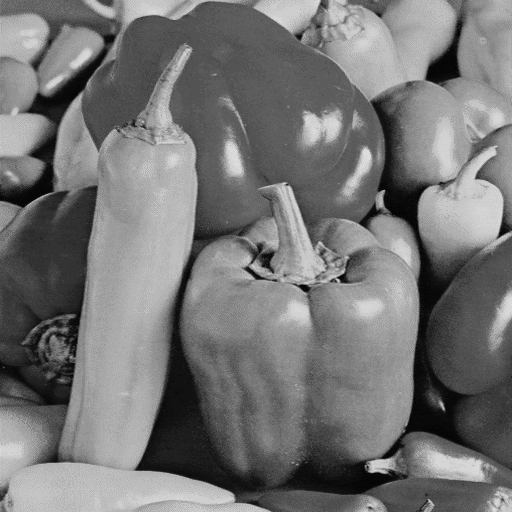
\includegraphics[width=0.41\textwidth]{chapters/medianfilter/images/peppers/peppers_gray.png}}
\subcaptionbox{Noisy}{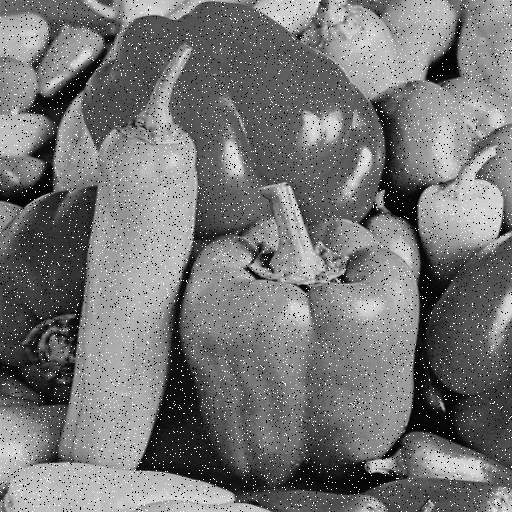
\includegraphics[width=0.41\textwidth]{chapters/medianfilter/images/peppers/peppers_gray_noisy.png}}
\subcaptionbox{Naïve}{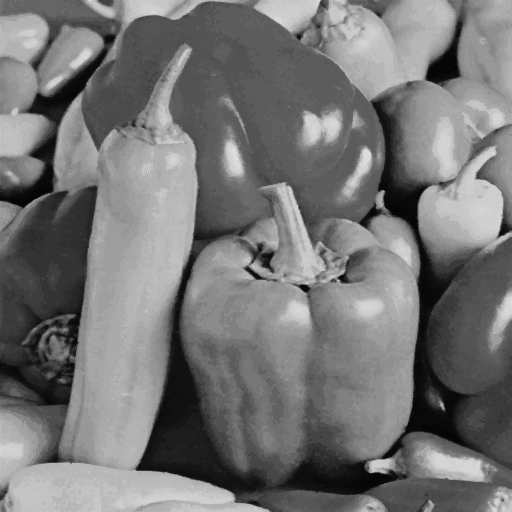
\includegraphics[width=0.41\textwidth]{chapters/medianfilter/images/peppers/naive_peppers_gray_noisy_3.png}}
\subcaptionbox{Bräunl}{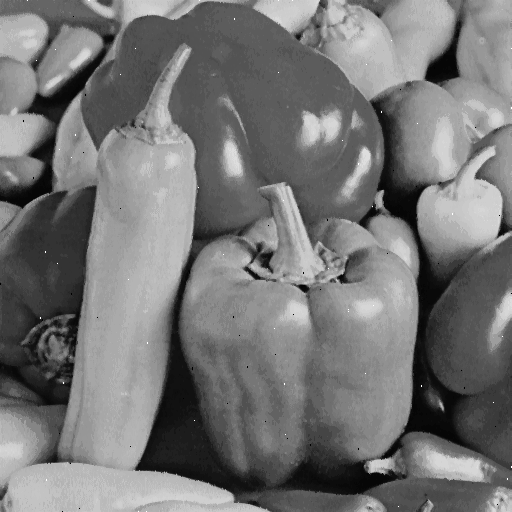
\includegraphics[width=0.41\textwidth]{chapters/medianfilter/images/peppers/braunl_peppers_gray_noisy_3.png}}
\subcaptionbox{\gls{cml}}{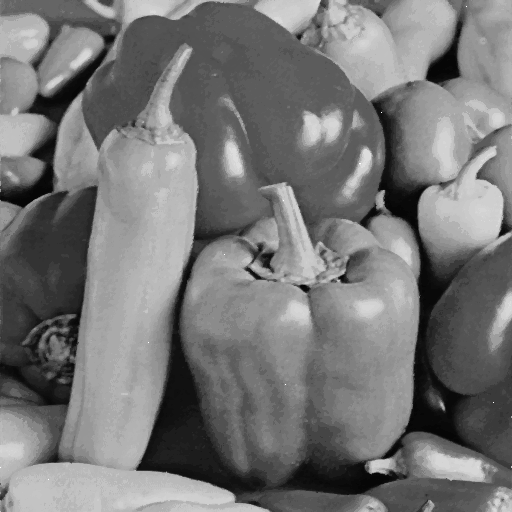
\includegraphics[width=0.41\textwidth]{chapters/medianfilter/images/peppers/cml_peppers_gray_noisy_3.png}}
\caption[The classic grayscale `peppers' image, before and after processing]{\label{fig:median:peppers}The classic greyscale `peppers' image, before and after processing.  (a) is the original image; (b) is the image with random salt \& pepper noise introduced; (c) is the result of processing the image using the naïve algorithm; (d) is the result of processing the image using the Br\"{a}unl-inspired algorithm; (e) is the result of processing the image using the \gls{cml} algorithm}
\end{figure}

\begin{table}
\centering
\caption[Peak signal-to-noise for the very small image]{Peak signal-to-noise ratio for the very small image (measured in \unit{\decibel})}
\label{tab:median:psnrvsmall}
\begin{tabular}{@{}lccccc@{}}
\toprule
\multicolumn{1}{c}{\textbf{Algorithm}} & \multicolumn{5}{c}{\textbf{Window size}}                                          \\
                                       & 3              & 5              & 7              & 9             & 11             \\ \midrule
Bräunl                                 & 20.78          & 17.82          & 15.65          & 14.36         & 13.55          \\
\gls{cml}                                    & 25.98          & \textbf{21.85} & \textbf{18.62} & \textbf{16.40} & 14.99          \\
Naïve                                  & \textbf{27.03} & 21.74          & 18.55          & 16.39         & \textbf{15.02} \\ \bottomrule
\end{tabular}
\end{table}

\begin{table}
\centering
\caption[Peak signal-to-noise for the peppers image]{Peak signal-to-noise ratio for the peppers image (measured in \unit{\decibel})}
\begin{tabular}{@{}lccccc@{}}
\toprule
\multicolumn{1}{c}{\textbf{Algorithm}} & \multicolumn{5}{c}{\textbf{Window size}}                                          \\
                                       & 3              & 5              & 7              & 9              & 11            \\ \midrule
Bräunl                                 & 28.76          & 27.35          & 25.27          & 23.94          & 22.82         \\
\gls{cml}                                    & 31.85          & 31.07          & 29.8           & 28.56          & 27.42         \\
Naïve                                  & \textbf{32.79} & \textbf{31.25} & \textbf{29.87} & \textbf{28.63} & \textbf{27.50} \\ \bottomrule
\end{tabular}
\label{tab:median:psnrpeppers}
\end{table}

\begin{table}
\centering
\caption[Peak signal-to-noise for the small image]{Peak signal-to-noise ratio for the small image (measured in \unit{\decibel})}
\label{tab:median:psnrsmall}
\begin{tabular}{@{}lccccc@{}}
\toprule
\multicolumn{1}{c}{\textbf{Algorithm}} & \multicolumn{5}{c}{\textbf{Window size}}                                          \\
                                       & 3              & 5              & 7             & 9              & 11             \\ \midrule
Bräunl                                 & 32.83          & 32.34          & 30.74         & 29.73          & 28.94          \\
\gls{cml}                                    & 36.62          & 34.25          & 32.66         & 31.57          & 30.71          \\
Naïve                                  & \textbf{37.83} & \textbf{34.31} & \textbf{32.7} & \textbf{31.65} & \textbf{30.81} \\ \bottomrule
\end{tabular}
\end{table}

\begin{table}
\centering
\caption[Peak signal-to-noise for the medium image]{Peak signal-to-noise ratio for the medium image (measured in \unit{\decibel})}
\begin{tabular}{@{}lccccc@{}}
\toprule
\multicolumn{1}{c}{\textbf{Algorithm}} & \multicolumn{5}{c}{\textbf{Window size}}                                           \\
                                       & 3              & 5              & 7              & 9              & 11             \\ \midrule
Bräunl                                 & 32.98          & 32.65          & 31.59          & 30.91          & 30.36          \\
\gls{cml}                                    & 36.72          & \textbf{34.15} & \textbf{32.98} & \textbf{32.26} & \textbf{31.73} \\
Naïve                                  & \textbf{37.16} & 34.07          & 32.96          & \textbf{32.26} & \textbf{31.73} \\ \bottomrule
\end{tabular}
\label{tab:median:psnrmedium}
\end{table}

Examination of the reported memory statistics (please see the GitHub repository for details) appears to show that the maximum amount of memory allocated during processing for the \gls{cml} algorithm stays roughly constant across window sizes for each image size, and in fact on larger window sizes it is the most memory efficient.  The naïve algorithm quickly grows to consume the most memory at larger window sizes for each image size, suggesting that it likely derives some of its comparative speed at the cost of greater space complexity, while Bräunl sits in the middle.  Conversely, \gls{cml} generates by far the most garbage collection events, which may help explain its relative sluggishness.

\section{Discussion}

The algorithms developed and presented here are not necessarily optimal for the purpose.  They largely handle each pixel separately, or combine them into arrays on-the-fly.  This ignores the possibility of exploiting data-parallelism to improve throughput, and instead relies only on the separate CPU cores to provide parallelism.

It is unclear how much the mechanics underlying these implementations (\ie{} the .NET Core and \hopac{} systems) attempt to maximise use of the processor cache.  Efficient use of the cache can contribute significantly to an optimised version of an algorithm outperforming, a simplistic version by an order of magnitude or more \cite{Ragan-Kelley2017}.  No attempt was made manually to ensure good practices, such as tiling or striping \cite{Midkiff2012}.

The \gls{cml} approach used in essence instantiates a \gls{pe} for each pixel, each of which must be scheduled to run at some point --- concurrent with another \gls{pe} in the case of synchronous message passing.  It is possible that this surfeit of separate logical threads may induce excessive switching costs, and perhaps promote wasted time, with threads regularly polling their channel and their neighbours'.  Careful improvements to this and the use of the cache might lead to significant gains in speed.

In terms of the code itself also, \gls{cml} appears to be the worst.  The program requires roughly double the number of lines of the naïve program, and is arguably much less `clean' or `readable'.  Reinterpreting the \gls{medianfilter} in terms of \glsxtrlong{csp} has not yielded a structural improvement nor simplified the programming task.  Combined with the running time results above, this suggests that the \gls{cml} approach is actively counter-productive for implementing \glspl{mwt}, at least when using \hopac{}.

Basic profiling of the \gls{cml}-based implementation appears to show that more than half of the runtime of the program was spent inside the function for giving a value over a channel, and functions called by it.  Furthermore, according to this profiling, almost 40\% of the total running time of the algorithm is taken up specifically by low-level memory management functions inside the depths of the .NET Core system.  Considering that some of these functions \fxwarning{ref?}{are written in hand-optimised assembly}, the fact they account for so much of the running time appears to suggest that memory use is poorly handled in the tested implementation.

\Glspl{mwt} are generally relatively simplistic processes, typically consisting simply of combining values from the pixel array, and which can be programmed in a straightforward fashion.  More sophisticated programming techniques may simply `get in the way' and introduce unnecessary overheads, which appears to have happened here.  Furthermore, the \gls{medianfilter} can largely be broken down into arithmetic and logical operations amenable to vectorisation (\eg{} \cite{Sanchez2012,Perreault2007}), which the \gls{cml} approach currently ignores entirely.

\subsection{Experimental Limitations}
There are two identifiable threats to validity, both regarding the `quality' of the programming involved.  .NET Core, as a widely used open-source compiler and runtime system, and which has likely had millions of man-hours invested in it, is presumably of high quality and fast in most cases.  That is not necessarily the case with \hopac{}.  While it is open source, and moderately well-known in the \fsharp{} community, the amount of time spent on optimising it is likely nowhere close to that spent on .NET Core.  Consequently, \hopac{} itself may present significant bottlenecks while performing the \gls{mwt}.

The other threat to validity (as with all performance-focused experiments) is the skill of the end programmer.  The author was new to the \hopac{} library at the start of this work, and inferior design choices may have been made unwittingly.  It was, however, suggested during personal communication with one of the maintainers and fellow users of the \hopac{} library that the \gls{cml} approach may simply be a poor fit to pixel-wise image processing tasks.

Fundamentally, the results achieved here, as with most implementation exercises, succeed or fail in large part on the skill, knowledge and effort of the programmers involved.  The use of other libraries may lead to better results.  Other parallel implementations of \gls{cml} exist, such as Concurrent Haskell \cite{Chaudhuri2009}, Manticore \cite{Reppy2009a} and Fibers\footnote{\url{https://github.com/wingo/fibers}} for Guile Scheme, but have not been assessed for this work.

\section{Summary}
The use of a \gls{cml} approach to image processing was explored in this \namecref{chap:median}, in particular as applied to the \gls{medianfilter} \gls{mwt} operation.  The measured results suggest that it is much worse than using a simple, naïve nested \texttt{for loop}s approach.  The reason for this appears to be related primarily to overhead from the synchronous communications, especially in regard to memory allocations and garbage collections.  This may be an issue with the \gls{cml} style in general, or it may be an issue related to the \gls{cml} library used or the programming of the algorithms tested here.  More work is required to determine this for certain.  \Gls{cml} does appear to provide one advantage, however, in that with larger window sizes it seemingly has the lowest peak space requirement.

A \gls{cml} approach where a separate \gls{pe} is used to represent each pixel largely eliminates the possibility of taking advantage of data-parallel hardware, such as vector instructions of CPUs or \glspl{gpu}.  For situations where vector instructions are applicable, the \gls{cml} approach seems likely to be a poor choice.  It is not clear, however, how well this approach may or may not work for instances where the data types involved are more complex, or where there is a significant level of control flow involved.  Nor has there been any investigation so far into the practicality of assigning multiple pixels to a single \gls{pe}.
\glsresetall
\newcounter{rulesnumber}

% --------------------------------------------------------------
\chapter{\label{chap:nmp}Neighbourhood Message Passing}

\section{Introduction}
This \namecref{chap:nmp} presents a framework for passing messages between discrete points on a finite lattice, where each point updates its internal data (and thus the messages it sends) based on messages received.  Each point is uniquely connected to other points and so has its own \emph{neighbourhood}, being the specific other points it communicates with.  A key aspect of this \emph{\gls{nmp}} computation is that the messages to a given neighbour depend upon the messages received previously from \emph{all} neighbours, \emph{except} the neighbour to which the current message is sent.    This necessarily means that in \gls{nmp} each grid location must have at least two neighbours; a single neighbour cannot form a meaningful neighbourhood.  This \namecref{chap:nmp} focuses on the \emph{square grid lattice}
but the principles of \gls{nmp} apply equally to all lattices.%focuses on the \emph{square grid lattice} but \gls{nmp} applies equally to lattices of any shape, dimension, or connectivity.

In this \namecref{chap:nmp}, the individual computational units in the lattice are termed \emph{\glspl{pe}}.\footnote{The short form ``\gls{pe}'' is derived from “processing element'' in the same way that “pixel'' is derived from “picture element''.}  These are the logical base units for computation for \gls{nmp} and are represented by \gls{cps} \glspl{tlc}.  A visual example of the \gls{nmp} process for the \emph{\gls{fne}} on the square lattice is shown in \cref{fig:nmp:gridmessaging}.  A \gls{pe} in the grid received messages from its neighbours to the left, right, and bottom at generation \(t - 1\), and used the data from those messages to prepare its new message to be sent to the neighbour above at iteration \(t\).  The same is performed for every other neighbour too.

\begin{figure}
    \centering
    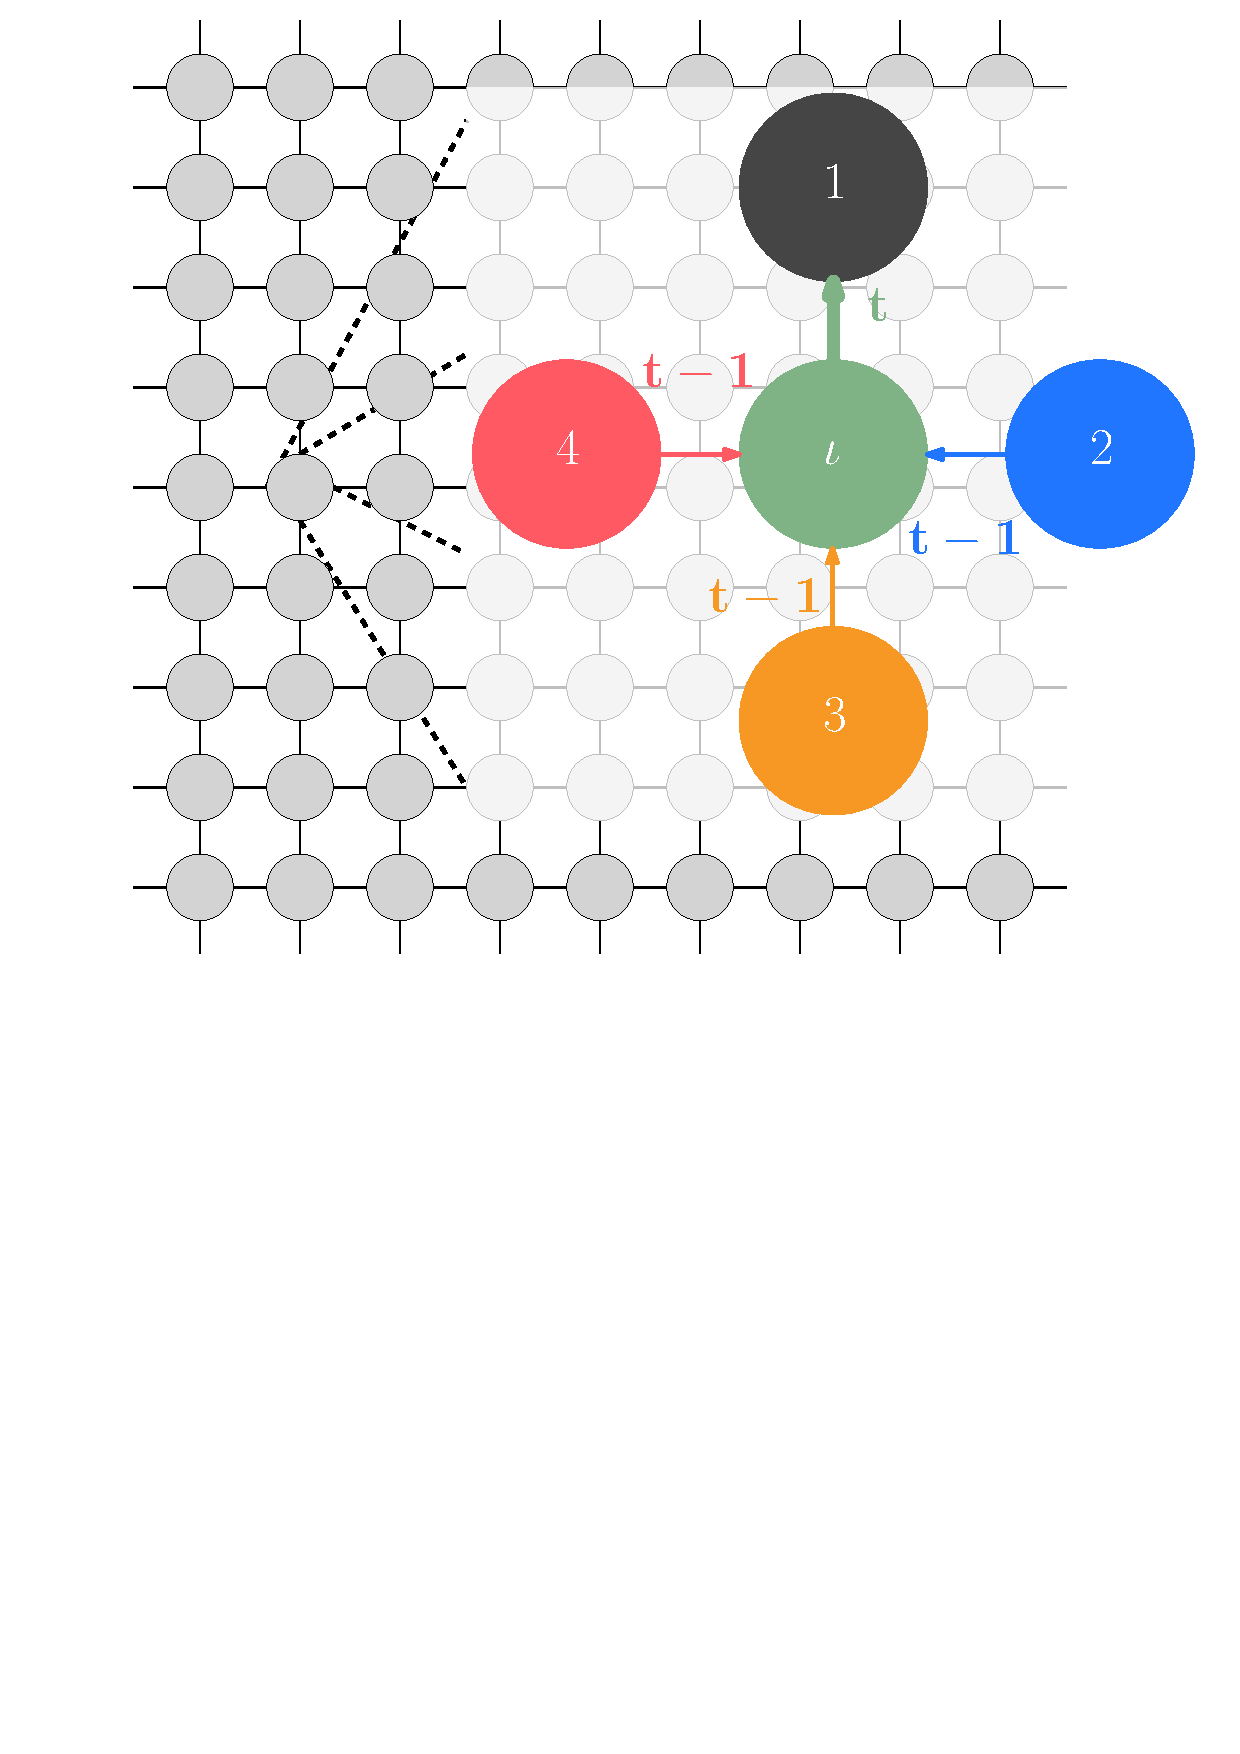
\includegraphics[keepaspectratio,width=1.0\linewidth]{chapters/nmp/images/bp_diagram_recoloured_iotacentre.pdf}
    \caption[Diagram of the central concept of \gls{fne} \glsxtrlong{nmp} on a grid]{Diagram of the central concept of \gls{fne} \gls{nmp} on a grid \cite{lbpmpsmpic}.  Each circle represents a \gls{pe}, labelled following the pattern of \cref{fig:nmp:iota_proxels_environment_oracle}.  The central \gls{pe} \(\iota\) needs to compute a new message to send at time \(t\) to \gls{pe} \(1\) above it, so it performs a computation to combine the results of the messages received from the other three neighbouring cells (\(2\), \(3\) \& \(4\)) at time \(t - 1\) (indicated by the thin and fat arrows).  The same is applied to every other neighbour, too.}
    \label{fig:nmp:gridmessaging}
\end{figure}

Conceptually, there are two distinct aspects of the \gls{nmp} process:
\begin{inparaenum}
\item the message passing itself, which occurs externally to \glspl{pe} over channels connected to other \glspl{pe}; and,
\item the data/message updates, which occur internally.
\end{inparaenum}
The focus of this \namecref{chap:nmp} is the external side, and communication with an oracle stands in for the internal computation, which is largely orthogonal to the inter-\gls{pe} communication.

There are (at least) two separate ways to model the \glspl{pe}' communication:  a \emph{\gls{gs}} system-wide view, where the states and steps taken occur across the system as a whole and every \gls{pe} carries out its operations simultaneously according to the same rules.  Or, a per-\gls{pe} view, where each \gls{pe} has its own state and advances \emph{asynchronously}\footnote{Recall from \vref{sec:back:syncasync} that the idea of asynchronicity used here follows the traditional concept from distributed computing, and so is \emph{different} to that sometimes used in other \gls{ps}.  Briefly, in the asynchronous model of distributed algorithms, external messages may take any arbitrary time (in \(\mathbb{R}\)) to reach their destinations \cite{Balanescu2011,Nicolescu2014,Lynch1996}, though internal updates are typically assumed to occur (near-)instantaneously.} without regard to others' objects, states, and rulesets.  This \namecref{chap:nmp} explores both and finds in the process that an intermediate third, \emph{\gls{ls}}, model arises naturally as a hybrid of the other two.

Modelling and implementation of \gls{nmp} proves surprisingly challenging.  The \gls{gs} form (\cref{sec:nmp:globalsync}) is reasonably simple.  It requires only nine rules, most of which have exactly one term on both the left-hand- and right-hand-sides, and none of which use \glspl{promoter} or \glspl{inhibitor} (see \cref{chap:cpsystems} for more on these concepts).

The challenge arises with the asynchronous version.  The possibility of messages from the same generation arriving at different times necessitates bookkeeping.
% It is necessary to track the sending neighbour from which each message for a given generation is received, to decide which neighbour(s) the current \gls{pe} is now ready to send a new outgoing message.
\Glspl{pe} must track from which neighbours messages have been received for a given generation, to decide to which neighbours the \gls{pe} is ready to send a new message.
This leads to inescapable complexity and the undesirable possibility of deadlock through unsuitable design.

% \Gls{nmp} shares similarities and overlaps with areas such as Cellular Automata, Gossip Protocols and Consensus Algorithms (see \eg{} [INSERT CITATIONS]). \Gls{nmp} is distinguished from these other areas in a few ways, however. Firstly, other approaches do not usually impose the ``\(n - 1\) neighbours'' condition of message updates as found in \gls{nmp}. Secondly, in other areas messaging tends to be only a part of the process, whereas in \gls{nmp} it is the heart of it. Internal computation is only performed to aggregate/average the messages received from neighbours to prepare new messages. Thirdly, in \gls{nmp} neither a global nor local consensus is sought — the closest equivalent would be the (tautological) concept of individual consensus per \gls{pe}. Rather, the result of each \gls{pe} comprises one distinct part of the final result. Lastly, often in these other areas, the neighbours are selected at random, rather than being a neighbourhood arising naturally from the structure of the modelled problem. Generalisation across these fields may be possible, but is not pursued further.
\Gls{nmp} shares similarities and overlaps with areas such as Cellular Automata, Gossip Protocols and Consensus Algorithms (see, \eg{}, \cite{Deserable2012,Hollander2015}).  \Gls{nmp} is distinguished from these other areas in a few ways, however.  Firstly, other approaches do not usually impose the ``\(n - 1\) neighbours'' condition of message updates as found in \gls{nmp}.  Secondly, in other areas messaging tends to be only a part of the process, whereas in \gls{nmp} it is the heart of it.  Internal computation is only performed to aggregate/average the messages received from neighbours to prepare new messages.  Thirdly, neither a global nor local consensus is sought in \gls{nmp} --- the closest equivalent would be the (tautological) concept of individual consensus per \gls{pe}.  Instead, the result of each \gls{pe} comprises one distinct part of the final result.  Lastly, often in these other areas, the neighbours are selected at random rather than being a neighbourhood arising naturally from the structure of the modelled problem.  Generalisation across these fields may be possible but is not pursued further.

This \namecref{chap:nmp} begins by describing a straightforward \gls{gs} \gls{nmp} system.  Then, it provides an asynchronous \gls{pe}-specific version of the same, followed by an adaptation of the asynchronous system to a \gls{ls} system. Next is a short example of a potential evolution of the asynchronous system to clarify its operation.  Lastly, this \namecref{chap:nmp} analyses the asynchronous system and reports the results of comparative computer experiments for all three systems.  The analysis proves that the asynchronous system sends precisely the same number of messages as the \gls{gs} system (one per generation per neighbour) but that the data used to compute new messages may vary slightly depending on the ordering of messages received.  Furthermore, the empirical results verify the operation of the asynchronous system and support the hypothesis that the \gls{ls} and asynchronous systems are faster than an equivalent \gls{gs} version.

\subsection{Belief Propagation}

This \namecref{chap:nmp} was originally motivated by attempts to model \emph{\gls{lbp}} for \gls{sm} (see \eg{} \cite{Blake2011,Felzenszwalb2011,Sun2003}) in \gls{cps}.  \emph{\Gls{bp}} was originally introduced to solve inference problems in AI on graphs \cite{Pearl1982} by treating the nodes as communicating objects, which passed messages backwards and forwards, updating their outgoing messages based on the incoming ones, to solve the problem.  The original formulation relied upon the graphs having a tree structure, however.  Each node would receive a message from its parent, pass that to its children, receive new messages back from the children and pass its own newly computed message back to its parent based on those received from the children.

In the case of \gls{sm}, the output is a (typically rectangular) grid representing an output image.  This means that the computation, sited on this grid, is inherently non-tree-structured.  Instead, each output node is connected to its neighbours -- usually in a \gls{fne} -- which means that messages travel in loops on the grid.  To deal with this situation, \gls{bp} was adapted to \gls{lbp}, which was first applied to \gls{sm} by \citeauthor{Sun2003} \cite{Sun2003}.  The algorithm was then significantly improved upon by \citeauthor{Felzenszwalb2006} \cite{Felzenszwalb2006}.

\Gls{nmp}, as described in this \namecref{chap:nmp}, can simulate \gls{lbp} effectively, and \cref{sec:nmp:example,sec:nmp:analysis,sec:nmp:experiments} focus on the \gls{fne}.  The main adaptation required is to replace the oracle with appropriate computations for \gls{lbp} \gls{sm}.  \Gls{nmp} can be generalised further, however, to perform other computations or use other communication arrangements besides the \gls{fne}.  While this work was originally inspired by \gls{lbp}, it is a generic framework for \emph{any} computations that may be modelled with communication on a lattice, when the outgoing message to one neighbour depends on the messages received from all other neighbours.
\section{\label{sec:nmp:systemwide}System-wide-synchronicity Messaging}

\cpresetrulenumber

This \namecref{sec:nmp:systemwide} presents the first \gls{nmp} variant, wherein the entire system evolves as one, and every \gls{pe} executes the same rule(s) simultaneously.  For the entirety of this \namecref{chap:nmp}, assume that all \glspl{pe}, channels and the oracle (\(o\)) behave correctly and follow their respective protocols, without faults, corruptions, lost messages, \etc{}  This significantly simplifies the presented systems by allowing the omission of error handling concepts and describing only the intended operation.

\begin{figure}
    \centering
    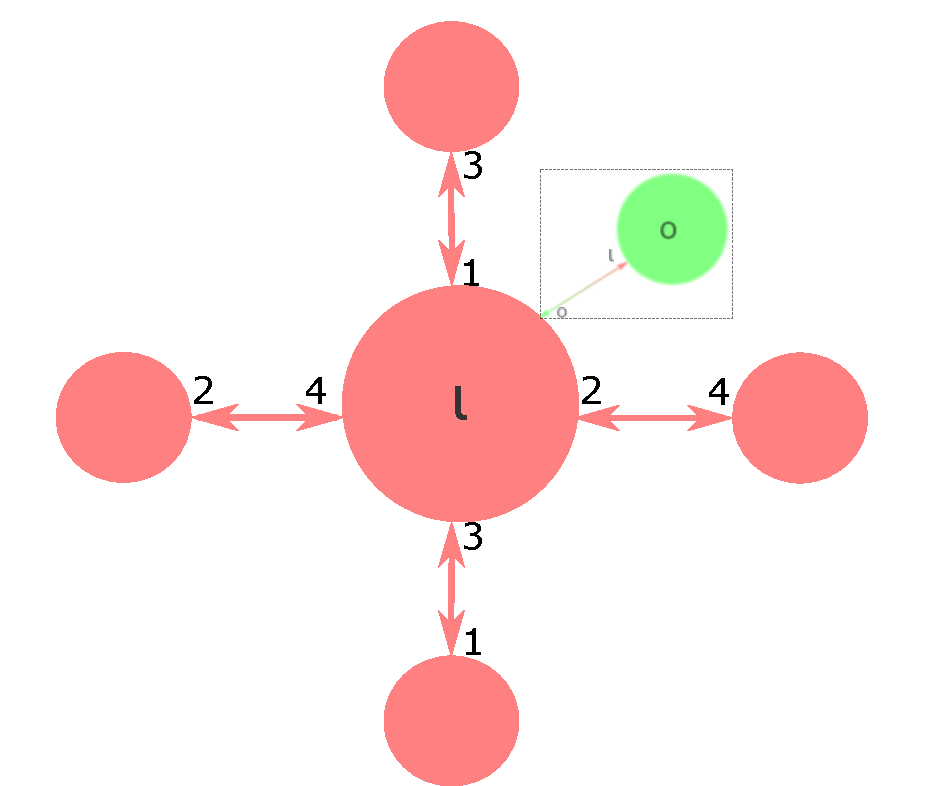
\includegraphics[width=0.9\textwidth]{chapters/nmp/images/iota_proxels_oracle_v7.pdf}
    \caption[The communication topology of a \glsxtrlong{nmp} system from the perspective of an arbitrary \glsxtrshort{pe} in a \gls{fne} arrangement]{The communication topology of the system from the perspective of an arbitrary \gls{pe} in a \gls{fne} arrangement.}
    \label{fig:nmp:iota_proxels_environment_oracle}
\end{figure}

The layout of the system, from the perspective of an arbitrary \gls{pe} in a \gls{fne}, is depicted in \cref{fig:nmp:iota_proxels_environment_oracle}.  The central circle is this \gls{pe} and is labelled with \(\iota\) to represent its ID in the overall system.  It is connected to each neighbour and the oracle by two-way channels.  The neighbours themselves are anonymous, but \(\iota\)'s end of each channel is labelled with a number from 1-4, representing the neighbours who are expected to sit above, to the right, below and to the left of the central \gls{pe}, respectively.  The oracle is smaller, blurred and surrounded with a dashed line, to reflect that it is a stand-in for an unspecified process that ordinarily would take place \emph{inside} the \gls{pe}.

In the current approach, each \gls{pe} has \emph{no} direct knowledge of its neighbouring \glspl{pe}.  Instead, it interacts with channels that connect to those neighbours; the channels interpose between the \glspl{pe}.  Furthermore, each label for a neighbour in a \gls{pe} is \emph{not} the system's ID for that neighbour, but the \gls{pe}'s label for a connecting channel endpoint.  Nevertheless, as a shortcut, \glspl{pe} will simply be referred to as communicating with their neighbours.  Messages exchanged by \glspl{pe} are termed \emph{\gls{nm} messages}, while messages exchanged with an oracle may be referred to as \emph{\gls{oq} messages}.

In the \gls{gs} version, the entire system evolves in lock-step, and thus is always in the same phase and \gls{cps} state.  The evolution follows a basic process, consisting of three conceptually distinct phases, the first two of which may be repeated.  Specifically, the system proceeds as follows (the rules are listed in \vref{ruleset:nmp:systemwide} and explained in \vref{sec:nmp:systemwide:rulesdesc}):

\begin{enumerate}
    % \item\label{enumitem:nmp:init} Initialisation (Rules \cpruleref*{rule:nmp:systemwide:recvcounter} \& \cpruleref*{rule:nmp:systemwide:recvinput})
    \item\label{enumitem:nmp:pu} \Gls{oq} (Rules \cpruleref*{rule:nmp:systemwide:loopdecrement}, \cpruleref*{rule:nmp:systemwide:sendtooracle} \& \cpruleref*{rule:nmp:systemwide:recvfromoracle})
    \item\label{enumitem:nmp:nm} \Gls{nm} (rule \cpruleref*{rule:nmp:systemwide:antiport})
    \item\label{enumitem:nmp:final} \textsf{Finalisation} (Rules \cpruleref*{rule:nmp:systemwide:loopend}, \cpruleref*{rule:nmp:systemwide:oraclefinalise} \& \cpruleref*{rule:nmp:systemwide:end})
\end{enumerate}

% This progression is depicted as a state machine in \cref{fig:nmp:systemwidestatemachine}.  State \(s_1\) covers the initialisation phase; \(s_2\) and \(s_3\) the \gls{oq} phase; \(s_4\) the \gls{nm} phase; and \(s_5\) and \(s_6\) the finalisation phase.  State \(s_7\) is the halting phase of the system's evolution.  In an application of \gls{nmp} phases \ref{enumitem:nmp:init}, \ref{enumitem:nmp:nm} and \ref{enumitem:nmp:final} will not change.  Only phase \ref{enumitem:nmp:pu} would be replaced.  The system's evolution is sketched at a high level in \cref{alg:nmp:systemwide2}.

\Cref{fig:nmp:systemwidestatemachine} depicts this progression as a state machine.  States \(s_1\) and \(s_2\) cover the \gls{oq} phase; \(s_3\) the \gls{nm} phase; and \(s_4\) and \(s_5\) the \textsf{finalisation} phase.  State \(s_6\) is the halting state of the system's evolution.  In an application of \gls{nmp} phases \ref{enumitem:nmp:nm} and \ref{enumitem:nmp:final} will not change.  Only phase \ref{enumitem:nmp:pu} is replaced.  The system's evolution is sketched at a high level in \cref{alg:nmp:systemwide2}.

The \gls{oq} phase is when each \gls{pe} performs its internal computation. As mentioned earlier, these computations are problem-dependent and thus cannot be modelled generically. Instead, this \namecref{chap:nmp} uses communication with an oracle assigned to each \gls{pe} to simulate this aspect of \gls{nmp}. The \gls{nm} phase is the main focus of this work. This is where \glspl{pe} exchange messages with their neighbours, based on data received earlier from other neighbours. The \textsf{finalisation} phase occurs after each \gls{pe} reaches a stopping point. At this point, each \gls{pe} performs a final computation to determine its output for the lattice, incorporating the latest data received from neighbours.

\begin{figure}
    \centering
    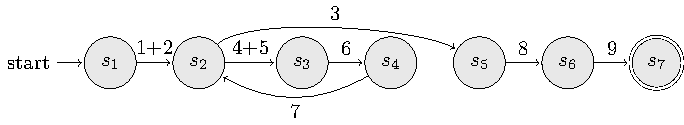
\includegraphics{chapters/nmp/images/systemwidestatemachine.pdf}
    \caption[State machine of the progression of the system-wide \glsxtrlong{nmp} \gls{cps} rules.]{State machine of the progression of the system-wide \gls{nmp} \gls{cps} rules.  The vertices are labelled with states and the arcs with the rule(s) which cause the state transitions.}
    \label{fig:nmp:systemwidestatemachine}
\end{figure}

\begin{algorithm}
\DontPrintSemicolon
\KwIn{Iteration counter \(i\) and array \(v\) of initial data}
\KwOut{Final result \(z\)}
\SetKwFor{pForEach}{parallel foreach}{do}{endfch}
\Begin{
    \tcc{\(\alpha \Leftarrow \langle \beta \rangle\) denotes receiving object \(\alpha\) on channel \(\beta\);\newline\(\gamma \Rightarrow \langle \delta \rangle\) denotes sending object \(\gamma\) on channel \(\delta\);\newline\(\epsilon \Leftrightarrow \langle \phi \rangle\) denotes antiport exchange, sending \emph{and} receiving (swapping) objects \(\epsilon\) on channel \(\phi\).}\;
    
    % \tcc{Initialisation}
    % \(i \Leftarrow \langle e \rangle\)\;
    % \lpForEach{\((x,d) \Leftarrow \langle e \rangle\)}{\(v[x] \gets d\)}\;
    
    \While{\(i > 0\)}{
        \tcc{\Glsentrylong{oq}}
        \(i \gets i - 1\)\;
        \pForEach{\(x \in \{1, 2, 3, 4\}\)}{
            \(w[x] \gets v[x]\)\;
            \(w[x] \Rightarrow \langle o \rangle\)
        }
        \lpForEach{\((x,d) \Leftarrow \langle o \rangle\)}{
            \(v[x] \gets d\)\
        }
        
        \;\tcc{\Glsentrylong{nm}}
        \lpForEach{\(x \in \{1, 2, 3, 4\}\)}{\(v[x] \Leftrightarrow \langle x \rangle\)}
    }
    \;\tcc{\textsf{Finalisation}}
    \pForEach{\(x \in \{1, 2, 3, 4\}\)}{
        \(w'[x] \gets v[x]\)\;
        \(w'[x] \Rightarrow \langle o \rangle\)
    }
    \(z \Leftarrow \langle o \rangle\)\;
    % \(z \Rightarrow \langle e \rangle\)
}
\caption[Pseudocode of the \glsxtrlong{nmp} process in the \gls{gs} system]{\label{alg:nmp:systemwide2}Pseudocode description of the process for an individual \gls{pe} in the \gls{gs} system}
\end{algorithm}

Assume before the start of the system's evolution that the correct number of \glspl{pe} are already in place, and they each contain an appropriately initialised iteration counter and their relevant channel endpoints only.  Everything else required by each \gls{pe} will be supplied by the oracle, or generated by rules during the \gls{pe}'s evolution.  The rules for the \gls{gs} system are listed in \cref{ruleset:nmp:systemwide} and explained in \cref{sec:nmp:systemwide:rulesdesc}.  This \namecref{sec:nmp:systemwide} first defines the \gls{gs} \gls{nmp} system, explains the intended operation of the \gls{ruleset}, then describes each of the ground terms used.

\subsection{System Definition}
Recall from \cref{sec:cps:formaldescriptions} that a given \gls{cps} implementation can be defined as a 6-tuple:

\cptuple{\text{NMP-GS}}{\cpset{\sigma_1, \dots, \sigma_{\text{max}}}}{A}{O}{\text{\cref{ruleset:nmp:systemwide}}}{\cpset{s_1, s_2, s_3, s_4, s_5, s_6}}{s_1}

\(T\) is a set of \glspl{tlc}, each representing a single \gls{pe}, numbered from one to the total size of the lattice.  These numbers correspond to the \(\iota\) of \cref{fig:nmp:iota_proxels_environment_oracle}.  \(A\) is the set of all terms defined in \cref{sec:nmp:systemwide:definitions}.  Each \gls{pe}'s starting multiset in \(O\) is a generation counter functor \(i\) and its set of initial data \(V\).

\subsection{\label{sec:nmp:systemwide:rulesdesc}Description of Rules}

\begin{cprulesetfloat}
    \begin{cpruleset}
        % % Receive maximum generation counter
        % \cprule[rule:nmp:systemwide:recvcounter]{s_1}{\cprecv{\cpfunc{i}{I}}{e}}{\cponce}{s_2}{\cpfunc{i}{I}}
        
        % % Receive inputs from environment
        % \cprule[rule:nmp:systemwide:recvinput]{s_1}{\cprecv{\cpvq{X}{D}}{e}}{\cpmaxpar}{s_2}{\cpvq{X}{D}}
        
        \\
        
        % Else move to finishing
        \cprule[rule:nmp:systemwide:loopend]{s_1}{i(\lambda)}{\cponce}{s_4}{}
        
        % Decrement iterator
        \cprule[rule:nmp:systemwide:loopdecrement]{s_1}{i(I\cpundig)}{\cponce}{s_2}{i(I)}
        
        % Send to oracle
        \cprule[rule:nmp:systemwide:sendtooracle]{s_1}{\cpvq{X}{D}}{\cpmaxpar}{s_2}{\cpsend{\cpvqw{X}{D}}{o}}
        
        % Receive from oracle
        \cprule[rule:nmp:systemwide:recvfromoracle]{s_2}{\cprecv{\cpvqw{X}{D}}{o}}{\cpmaxpar}{s_3}{\cpvq{X}{D}}
        
        \\
        
        % Exchange messages
        \cprule[rule:nmp:systemwide:antiport]{s_3}{\cpvq{X}{D} & & &\\ & \cpantirecv{\cpvq{\_}{D'}}{X}}{\cpmaxpar}{s_1}{\cpvq{X}{D'} &\\ & & & & \cpantisend{\cpvq{X}{D}}{X}}
        
        \\
        
        % Send to oracle (finalisation)
        \cprule[rule:nmp:systemwide:oraclefinalise]{s_4}{\cpvq{X}{D}}{\cpmaxpar}{s_5}{\cpsend{w'\perfectunary{IncreaseHeight}{(}{)}{X}\perfectunary{IncreaseHeight}{(}{)}{D}}{o}}
        
        % Oracle returns results
        \cprule[rule:nmp:systemwide:end]{s_5}{\cprecv{\cpfunc{z}{Z}}{o}}{\cpundig}{s_6}{\cpfunc{z}{Z}}
        
    \end{cpruleset}
    \caption[Complete \gls{ruleset} for \gls{gs} \glsxtrlong{nmp}]{\label{ruleset:nmp:systemwide}Complete \gls{ruleset} for \gls{gs} \gls{nmp}, using an oracle to perform update computations}
\end{cprulesetfloat}

\begin{enumerate}
    % \item Receive \(I\), the maximum generation count or the number of rounds of message passing each \gls{pe} should engage in.\footnote{In general with \gls{nmp} a fixed number of generations is not the only way to determine when \gls{nm} should cease, but other methods tend to be specific to the problem at hand.   Therefore, a generation count is the only one presented here.  It should be applicable no matter the computation performed.}
    % \item Receive from the environment \gls{nm} messages \(v(X)(D)\), being the \gls{pe}'s initial data for its neighbours.
    \item If \(i\) is empty, continue to the \textsf{finalisation} phase.
    \item Decrement \(i\) when sending \(w\) messages to the oracle for \gls{oq}.
    \item Convert the \(v\) messages into \(w\) messages and send them to the oracle to compute the new messages to send to neighbours.
    \item Receive back new \(w\) objects from the oracle and convert them to \(v\) objects.
    \item Swap \(v\) messages with each neighbour \(X\), using antiport communication (see \cref{sec:cps:antiport}).
    \item Send the \(v\) objects as \(w'\) to the oracle for \textsf{finalisation} computation.
    \item Receive the final result \(\cpfunc{z}{Z}\) from the oracle and halt.% and send it to the environment.\footnote{One might wonder why the oracle could not simply emit the final result directly into the environment.  Strictly speaking, that would be reasonable in the context of this system, but bear in mind that the oracle is simply an abstraction over an arbitrary computation, which would take place \emph{inside} the \gls{pe}.}
\end{enumerate}

\subsection{\label{sec:nmp:systemwide:definitions}Definitions of Terms}

\paragraph{Atoms}
\begin{description}
    % \cptermdef{e}{The label of the channel used to communicate with the environment.}
    \cptermdef{o}{The label of the channel used to communicate with the oracle.}
    \cptermdef{\cpempty}{The \gls{cps} `empty' atom (see \cref{sec:cps:complexsymbols,sec:cps:natnums}).}
\end{description}

\paragraph{Functors}
\begin{description}
    \cptermdef{i}{A generation counter.  Used to count the number of generations of \gls{nm} remaining before moving to the \textsf{finalisation} phase.}
    \cptermdef{v}{The \(v\) compound terms described in \cref{sec:cps:compoundterms} \emph{except} without the generation counter --- the \(i\) counter serves the same purpose for the \gls{gs} variant.  These serve as \gls{nm} messages.}
    \cptermdef{w}{The same as the \(v\) terms, but used as messages to the oracle for \gls{oq}.}
    \cptermdef{w'}{The same as the above \(w\) objects, but marked to indicate to the oracle that they are to be used for \textsf{finalisation} rather than \gls{oq}.}
    \cptermdef{z}{Final output functor.  Holds the result of the \gls{pe}’s computation.}
\end{description}

\paragraph{States}
\begin{description}
    % \cptermdef{s_1}{Beginning state.  The \glspl{pe} receive their inputs from the environment.}
    \cptermdef{s_1}{The opening \gls{oq} phase state, where data are sent to the oracle and the generation counter is decremented.}
    \cptermdef{s_2}{Data update receipt state. Updated data are received back from the oracle.}
    \cptermdef{s_3}{\Gls{nm} state.  Messages are swapped with neighbours.}
    \cptermdef{s_4}{\textsf{Finalisation} phase transition state}
    \cptermdef{s_5}{State for transmission to the oracle for the final result, and awaiting its response.}
    \cptermdef{s_6}{State for receipt of the result from the oracle and halting of evolution.}
\end{description}
\section{\label{sec:nmp:pespecific}Processing Element-specific Asynchronous Messaging}
% \cpresetrulenumber

This \lcnamecref{sec:nmp:pespecific} presents a variant of the above system where the rules are applied in a \gls{pe}-specific manner and the \glspl{pe} run \emph{asynchronously} \cite{Balanescu2011,Nicolescu2014}, so that the steps of one \gls{pe} do not necessarily occur contemporaneously with those of another.\footnote{In this form, \gls{nmp} shares some obvious similarities with \Gls{csp} (\cref{subsec:back:csp}), \Glspl{actor} (\cref{subsec:back:actors}) and \Glspl{pram} (\cref{sec:back:othermodels}).}  

\begin{anfxwarning}{Keep and modify this paragraph, or delete it?}
There is no longer a single state spanning the entire system.  Instead, each \gls{pe} has its own state dictating its operation individually.  The same conceptual phases are kept, though the \gls{oq} and \gls{nm} phases are combined because they now may occur interleaved.  During the \gls{oq} \& \gls{nm} phase, each \gls{pe} independently works through a series of \label{pg:nmp:rounds}\emph{rounds}, following the typical idea of a round in theoretical asynchronous systems:  The \gls{pe} receives one or more messages, processes the received messages and updates its internal data, then sends out new messages based on the results.
\end{anfxwarning}

The most significant change from \cref{sec:nmp:systemwide} is the use of \emph{receipt tokens} and \emph{generation counts}.  Receipt tokens show that the \gls{pe} has received a message from a particular neighbour since the last time messages were sent.  This is vital to ensure that the correct number of messages are sent, and sent only after receiving appropriate messages from other neighbours.

In the \gls{gs} system, the received messages used to update the outgoing messages could always be assumed to have been sent during the same round as each other.  This is not the case under the asynchronous system, where a message may be sent out (and thus received) as soon as the necessary input messages have been received.  This has the potential to messages being used out-of-order, where a message from what would have been an earlier `round' is re-used inappropriately.  Thus, these messages are now tagged with a round number, termed here a \emph{generation} because each outgoing message is essentially the direct progeny of the messages received at the last generation.

The other change of note is that initialisation of the \glspl{pe} also differs slightly from \cref{sec:nmp:systemwide}.  Along with the channels, each \gls{pe} also starts with an adjacency list object, \(\cpfunc{a}{A}\), which holds a copy of the atoms for each neighbour/channel.

\begin{figure}
    \centering
    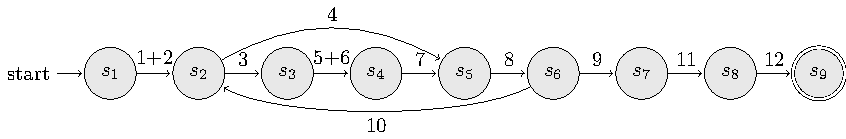
\includegraphics[width=1.0\textwidth]{chapters/nmp/images/proxelspecificstatemachine.pdf}
    \caption[State machine of the progression of the \glsxtrshort{pe}-specific \glsxtrlong{nmp} \gls{cps} rules]{State machine of the progression of the \gls{pe}-specific \gls{nmp} \gls{cps} rules.  The vertices are labelled with the states and the arcs with the rule(s) which cause that transition.}
    \label{fig:nmp:proxelspecificstatemachine}
\end{figure}

As with \cref{sec:nmp:systemwide}, this \lcnamecref{sec:nmp:pespecific} shows the progression of the system through its states in \cref{fig:nmp:proxelspecificstatemachine}.  In this system, an \gls{oq} \& \gls{nm} round can be regarded as the steps taken to proceed from state \(s_2\) until reaching \(s_2\) again.  Thus, receiving one or more messages, followed potentially by preparing and sending new messages, forms a round.  The initialisation phase is only rules \cpruleref*{rule:nmp:proxspec:initcounter} and \cpruleref*{rule:nmp:proxspec:recvinputs}.  The combined \gls{oq} and \gls{nm} phase is made up of rules \cpruleref*{rule:nmp:proxspec:makews} through \cpruleref*{rule:nmp:proxspec:recvfromneighs}, which involve the receipt of one or more messages with generation \(0 < g \leq I\) from neighbours, then preparation of new messages to send to neighbours through communicating with the oracle and forwarding the results of the oracle's computation to the relevant neighbours.  Lastly, rules \cpruleref*{rule:nmp:proxspec:finaloracle} and \cpruleref*{rule:nmp:proxspec:end} make up the finalisation phase.

\begin{algorithm}
\DontPrintSemicolon
\SetKwFunction{Uniq}{uniq}
\SetKwFunction{Perm}{permutations}
\SetKwFor{pForEach}{parallel foreach}{do}{endfch}
\SetKwBlock{Loop}{loop:}{}
\SetKw{KwOr}{or}
\SetKw{KwAnd}{and}
\SetKw{KwGoto}{goto}
\KwIn{Adjacency set \(A = \{1,2,3,4\}\)}
\KwOut{Final result, \(z\), sent to environment \(e\)}
\Begin{
    \tcc{
    \(a \Leftarrow \langle b \rangle\) denotes receiving object \(a\) on channel \(b\)\newline
    \(c \Rightarrow \langle d \rangle\) denotes sending object \(c\) on channel \(d\)
    }\;
    
    \tcc{Initialisation}
    \(R \gets \emptyset\)\;
    \(i \Leftarrow \langle e \rangle\)\;
    
    \tcc*[l]{* assume environment \(e\) sends all of these now}
    \pForEach{\((x, 0, d) \Leftarrow \langle e \rangle\)}{
        \(v[x] \gets (0,d)\)\;
        \(R \gets R \cup \{x\}\)
    }
    
    \;\tcc{\Glsentrylong{oq} \emph{and} \Glsentrylong{nm}}
    
    \Loop{
        \(W \gets \emptyset\)\;
        
        \pForEach{\((x,y,z,w) \in\) \Perm{\(A\)}}{
            \If{\(x \in R\) \KwAnd \(v[x].g < i\) \KwAnd \(v[x].g \leq v[y].g\) \KwAnd \(v[x].g \leq v[z].g\)}{
                \(W \gets W \cup (w,v[x].g+1, v[x].d \cup v[y].d \cup v[z].d))\)\label{line:nmp:rule3}
            }
        }
        
        \If{\(W \not= \emptyset\)}{
            \(W \gets\) \Uniq{\(W\)} \tcc*[l]{Multiset to set}
            \;
            \lpForEach{\((w, g, d) \in W\)}{\((w, g, d) \Rightarrow \langle o \rangle\)}
            \tcc*[l]{** assume oracle \(o\) returns all required messages}
            
            \lpForEach{\((w, g, d) \Leftarrow \langle o \rangle\)}{\((w, g, d) \Rightarrow \langle w \rangle\)}
            \(W \gets \emptyset\)
        }
        
        \(R \gets \emptyset\)\;
        \;
        \(b \gets\) \texttt{true}
        
        \lpForEach{\(x \in A\)}{\lIf*{\(v[x].g < i\)}{\(b \gets\) \texttt{false}}}
        \lIf{b}{\KwGoto break}\;
        
        \While{\(|R| = 0\)}{\label{line:nmp:recvwhile}
            \pForEach{\((x, g, d) \Leftarrow A\)}{\label{line:nmp:recvfor}
                \(v[x] \gets (g,d)\)\;
                \(R \gets R \cup \{x\}\)\;
            }
        }
        \KwGoto loop\;
    }
    \AlCapSty{\AlCapFnt break:}\;
    
    \;\tcc{Finalisation}
    
    \lpForEach{\(x \in A\)}{\(v[x] \Rightarrow \langle o \rangle\)}
    \(z \Leftarrow \langle o \rangle\)\;
    \(z \Rightarrow \langle e \rangle\)
}
\caption[Pseudocode description of the process for an individual \gls{fne} \glsxtrshort{pe} in the asynchronous system]{\label{alg:nmp:pespecific}Pseudocode description of the process for an individual \gls{fne} \gls{pe} in the asynchronous system}
\end{algorithm}

As with \cref{sec:nmp:systemwide}, this \lcnamecref{sec:nmp:pespecific} also supplies a pseudocode representation of the procedure in \cref{alg:nmp:pespecific}.  The pseudocode does not closely resemble \cref{ruleset:nmp:proxspec} in appearance.  Instead, the pseudocode is written to reflect best the meaning and intention of the rules while still relating it to the \gls{ruleset}.

An important assumption for this \gls{ruleset} is that the oracle returns all outstanding results together.  After a \gls{pe} sends one or more \gls{oq} messages to the oracle, it enters a blocking wait until it receives updated \gls{nm} messages back from the oracle.  One \gls{nm} message is expected per \gls{oq} message.  The oracle is assumed to return all these messages during one step, possibly waiting until it has finished computing new values for every message.  The same assumption is made for finalisation, and similarly, that the environment sends in all the initial messages during a single step.

In preparing the new \gls{oq} messages to go to the oracle, \cpruleref{rule:nmp:proxspec:makews} discards the information about which datum came from which neighbour (visible in \cref{line:nmp:rule3} in \cref{alg:nmp:pespecific}).  This is irrelevant for \gls{bp} \gls{sm}.  It might be relevant, however, to keep said information for a different computation.  One must bear this in mind when adapting the rules to their problem.  The changes needed are likely minor, but unexplored further here, as they are superfluous.

\subsection{System Definition}
Per the tuple definition from \cref{sec:cps:formaldescriptions}:

\cptuple{\text{NMP-Async}}{\cpset{\sigma_1, \dots, \sigma_{\text{max}}}}{A}{\cpset{\cpfunc{a}{A_t} \, | \, t \in T}}{\cref{ruleset:nmp:proxspec}}{\cpset{s_1, \dots, s_9}}{s_1}

\(T\) is a set of top-level cells, each representing a single \gls{pe}, numbered sequentially.  These numbers correspond to the \(\iota\) of \cref{fig:nmp:iota_proxels_environment_oracle}.  \(A\) is equal to the set of terms defined in \cref{sec:pespecific:definitions}.  Each \gls{pe}'s starting multiset in \(O\) is the appropriate channel endpoints and an adjacency list term \(a\), with contents \(A_t\) listing its neighbours specifically.  Every \gls{pe}'s \gls{ruleset} in \(R\) is either equal to that found in \cref{ruleset:nmp:proxspec}, or one which starts with that \gls{ruleset} as a base.  These latter \glspl{ruleset} drop terms from \cpruleref{rule:nmp:proxspec:makews} to adapt it to the relevant \gls{pe} having fewer than four neighbours (see \cref{sec:nmp:ruleslessthanfour}).

\subsection{Description of Rules}

\begin{cprulesetfloat}
    \begin{cpruleset}
    
        %%%%%%%%%%%%%  Initialisation  %%%%%%%%%%%%%
    
        % Receive inputs from environment
        \cprule[rule:nmp:proxspec:initcounter]{s_1}{\cprecv{\cpfunc{i}{I}}{e}}{\cponce}{s_2}{\cpfunc{i}{I}}
        
        \cprule[rule:nmp:proxspec:recvinputs]{s_1}{\cprecv{\cpvv{X}{\cpempty}{D}}{e}}{\cpmaxpar}{s_2}{\cpvv{X}{\cpempty}{D} & \\ & & & & \cpfunc{r}{X}}
        
        \\
        
        %%%%%%%%%%%%%  OQ & MP phase  %%%%%%%%%%%%%
        
        \cprule[rule:nmp:proxspec:makews]{s_2}{}{\cpmaxpar}{s_3}{\cpvw{W}{G\cpundig}{\cpfunc{d}{A}\,\cpfunc{d}{B}\,\cpfunc{d}{C}}}
        \cppromoter{\cpfunc{r}{X}}
        \cppromoter{\cpvv{X}{G}{A}}
        \cppromoter{\cpvv{Y}{G\cpdiscard}{B}}
        \cppromoter{\cpvv{Z}{G\cpdiscard}{C}}
        \cppromoter{\cpfunc{i}{G\cpundig\cpdiscard}}
        \cppromoter{\cpfunc{a}{\cpfunc{n}{X}\,\cpfunc{n}{Y}\,\cpfunc{n}{Z}\,\cpfunc{n}{W}}}
        
        \cprule[rule:nmp:proxspec:skiptorecv]{s_2}{}{\cponce}{s_5}{}
        
        \cprule[rule:nmp:proxspec:uniq]{s_3}{\cpvw{W}{\cpdiscard}{\cpdiscard}}{\cpmaxpar}{s_4}{}
        \cppromoter{\cpvw{W}{\cpdiscard}{\cpdiscard}}
        
        % Send to oracle
        \cprule[rule:nmp:proxspec:sendtooracle]{s_3}{\cpvw{W}{G}{D}}{\cpmaxpar}{s_4}{\cpsend{\cpvw{W}{G}{D}}{o}}
        
        % Receive from oracle & send to neighbour
        \cprule[rule:nmp:proxspec:recvfromoracle]{s_4}{\cprecv{\cpvw{W}{G}{D}}{o}}{\cpmaxpar}{s_5}{\cpsend{\cpvv{W}{G}{D}}{W}}
        
        % Clear all receipt tokens at the end of a send process
        \cprule[rule:nmp:proxspec:clearrs]{s_5}{\cpfunc{r}{\cpdiscard}}{\cpmaxpar}{s_6}{}
        
        % Transition to end if all generations complete
        \cprule[rule:nmp:proxspec:movetoend]{s_6}{}{\cponce}{s_7}{}
        \cpinhibitor{\cpvv{X}{G}{D}}
        \cppromoter{\cpfunc{i}{G\cpundig\cpdiscard}}
        
        %receive messages
        \cprule[rule:nmp:proxspec:recvfromneighs]{s_6}{\cprecv{\cpvv{\cpdiscard}{G\cpundig}{D}}{X} & & & \\ & \cpvv{X}{G}{\cpdiscard}}{\cpmaxpar}{s_2}{\cpvv{X}{G\cpundig}{D} &\\ & & & & \cpfunc{r}{X}}
        
        \\
        
        %%%%%%%%%%%%%  Finalisation %%%%%%%%%%%%%
        
        % Send to oracle
        \cprule[rule:nmp:proxspec:finaloracle]{s_7}{\cpvv{X}{G}{D}}{\cpmaxpar}{s_8}{\cpsend{w'\perfectunary{IncreaseHeight}{(}{)}{X}\perfectunary{IncreaseHeight}{(}{)}{G}\perfectunary{IncreaseHeight}{(}{)}{D}}{o}}
        
        % Oracle returns results which are immediately emitted to the environment
        \cprule[rule:nmp:proxspec:end]{s_8}{\cprecv{\cpfunc{z}{Z}}{o}}{\cpundig}{s_9}{\cpsend{\cpfunc{z}{Z}}{e}}
        
    \end{cpruleset}
    \caption[\Gls{ruleset} for the \glsfmttext{fne} \glsxtrshort{pe}-specific asynchronous \glsfmttext{nmp} system, for an inner \glsxtrshort{pe}]{\label{ruleset:nmp:proxspec}\Gls{ruleset} for the \gls{fne} \gls{pe}-specific asynchronous \gls{nmp} system, for an inner \gls{pe} (\ie{} one not on the border) and using an oracle to compute the data for outgoing messages}
\end{cprulesetfloat}

\begin{enumerate}
    \item Receive the \(\cpfunc{i}{I}\) input from the environment.
    \item Receive \(\cpvv{X}{\cpempty}{D}\) messages as inputs from the environment.
    \item Consider in turn all receipt tokens \(r\), if any (in any arbitrary order). For \(\cpfunc{r}{k_1}\) and \(\cpvv{k_1}{g_1}{\cpdiscard}\), compare generation number \(g_1\) against the generation numbers of all other current values \(\cpvv{k_j}{g_j}{\cpdiscard}, k_j \in \{k_2, k_3, k_4\} = \{1, 2, 3, 4\} \setminus \{k_1\}\). Without loss of generality, if \(g_1 \leq g_2, g_3\) \emph{and} \(g_1 < I\) (\ie{} the maximum generation count) then create a message \(w\) to send to the oracle for \gls{oq}.  This message has the data for \(k_1\), \(k_2\) and \(k_3\), which are used by the oracle in computing the new message to send to \(k_4\).  The generation count for this \(w\) message is \(g_1 + 1\).
    \item If there were no \gls{oq} messages generated by \cpruleref{rule:nmp:proxspec:makews}, then move straight to the process of testing for termination and receiving new messages.
    \item If \cpruleref{rule:nmp:proxspec:makews} resulted in the creation of more than one \gls{oq} message about a given neighbour, select one of those messages at random and delete the others.  The messages will be identical, but duplicates may arise due to the unification of different neighbours to \(Y\) and \(Z\) in \cpruleref{rule:nmp:proxspec:makews}.
    \item For each \gls{oq} message remaining after \cpruleref{rule:nmp:proxspec:uniq}, send said message to the oracle to compute the new corresponding outgoing \gls{nm} message.
    \item Forward newly prepared \gls{nm} messages \(v\) from the oracle to the relevant neighbour.
    \item Delete all extant receipt tokens after completing the relevant \gls{oq} \& \gls{nm} phase.
    \item If messages with a generation count equal to \(I\) have been received from every neighbour, transition to the finalisation phase.
    \item Receive a message \(\cpvv{\cpdiscard}{G}{D}\) from neighbour \(X\) and replace the current \(v\) object for \(X\) with it.  The neighbour label contained inside the message is overwritten with the current \gls{pe}'s label for the receiving channel.  Create a receipt token \(\cpfunc{r}{X}\).
    \item Send all the \gls{pe}'s \(v\) messages to the oracle, for the oracle to compute the final output for the \gls{pe}.
    \item Receive the computed final result from the oracle and send it to the environment.
\end{enumerate}

\subsection{\label{sec:pespecific:definitions}Definitions of Terms}

\paragraph{Atoms}
The same as in \cref{sec:nmp:systemwide}.

\paragraph{Functors}
\begin{description}
    \cptermdef{a}{Adjacency set.  Lists the neighbours of the \gls{pe} as a set of \(n\) functors.}
    \cptermdef{i}{Maximum generations counter.  Used slightly differently to \cref{sec:nmp:systemwide}.}
    \cptermdef{n}{Neighbourhood functor.  Stores the label for one of the channels/neighbours to which the current \gls{pe} is connected.}
    \cptermdef{r}{Receipt token, showing that a message was recently received from neighbour \(X\).}
    \cptermdef{v}{Serves as both the internal data stores and \gls{nm} messages of the system.  These are the \(v\) compound terms described in \cref{sec:cps:compoundterms}.}
    \cptermdef{w}{Identical in most respects to \(v\) functors, except used for messaging with the oracle instead of neighbouring \gls{pe}.  That is, these are \gls{oq}, rather than \gls{nm}, messages.}
    \cptermdef{w'}{Identical to \(w\), except marked to indicate to the oracle that the messages sent are to be used for finalisation computations instead of \gls{oq}.}
    \cptermdef{z}{Identical to the \(z\) in \cref{sec:nmp:systemwide}.}
\end{description}

\paragraph{States}
\begin{description}
    \cptermdef{s_1}{Environmental inputs receipt state.}
    \cptermdef{s_2}{Messaging round starting state.  If it is appropriate for the \gls{pe} to send new messages to its neighbours, then \gls{oq} messages are prepared and the sending process continues.  Otherwise, return to receiving once again.}
    \cptermdef{s_3}{Message send phase, part 1.  Drop any duplicate \gls{oq} messages referring to the same neighbour.   Send \gls{oq} messages to compute new outgoing \gls{nm} messages.}
    \cptermdef{s_4}{Receive the new \gls{nm} messages computed by the oracle, and forward them to the appropriate neighbour(s).}
    \cptermdef{s_5}{Receipt token deletion state.  Unconditionally delete all receipt tokens present.}
    \cptermdef{s_6}{Message receipt state.  When there are no messages to send, the \gls{pe} performs a `blocking' receipt (see \cref{sec:cps:blocking}) in this state until one or more of its neighbours send messages on the connecting channels.}
    \cptermdef{s_7}{Equivalent to state \(s_5\) in \cref{sec:nmp:systemwide}.}
    \cptermdef{s_8}{Equivalent to state \(s_6\) in \cref{sec:nmp:systemwide}.}
    \cptermdef{s_9}{Equivalent to state \(s_7\) in \cref{sec:nmp:systemwide}.}
\end{description}

\subsection{\label{sec:nmp:ruleslessthanfour}Rules for \glsfmtname{fne} Proxels with Fewer Than Four Neighbours}

\Cref{ruleset:nmp:proxspec} considers only the case where a \gls{pe} has exactly four neighbours.  This does not work correctly for those \glspl{pe} with three neighbours (\ie{} on the grid border, but not in a corner) or two neighbours (\ie{} in a grid corner).  The only adjustment necessary to handle these edge cases is to change the number of neighbours considered, specifically in \cpruleref{rule:nmp:proxspec:makews}.

These alternative rules are listed in \cref{ruleset:nmp:3alts} as {\cpruleref{rule:nmp:proxspec:makews}a} and {\cpruleref{rule:nmp:proxspec:makews}b} for the border and corner cases, respectively.  Assume henceforth that any \gls{nmp} system is constructed to handle the finite boundaries of the grid correctly by replacing the usual \cpruleref{rule:nmp:proxspec:makews} with the suitable alternative for edge \glspl{pe}.  \Cref{sec:nmp:example} uses rule {\cpruleref{rule:nmp:proxspec:makews}a} to simplify and shorten the example without neglecting the essential details.

\begin{cprulesetfloat}
    \begin{cpruleset}
        \cprulecustnum{s_2}{}{\cpmaxpar}{s_3}{\cpvw{W}{G\cpundig}{\cpfunc{d}{A} \, \cpfunc{d}{B}}}{\cpruleref*{rule:nmp:proxspec:makews}a}
        \cppromoter{\cpfunc{r}{X}}
        \cppromoter{\cpvv{X}{G}{A}}
        \cppromoter{\cpvv{Y}{G\cpdiscard}{B}}
        \cppromoter{\cpfunc{i}{G\cpundig\cpdiscard}}
        \cppromoter{\cpfunc{a}{\cpfunc{n}{X} \, \cpfunc{n}{Y} \, \cpfunc{n}{W}}}
        
        \\
        
        \cprulecustnum{s_2}{}{\cpmaxpar}{s_3}{\cpvw{W}{G\cpundig}{\cpfunc{d}{A}}}{\cpruleref*{rule:nmp:proxspec:makews}b}
        \cppromoter{\cpfunc{r}{X}}
        \cppromoter{\cpvv{X}{G}{A}}
        \cppromoter{\cpfunc{i}{G\cpundig\cpdiscard}}
        \cppromoter{\cpfunc{a}{\cpfunc{n}{X} \, \cpfunc{n}{W}}}
        
    \end{cpruleset}
    \caption[Alternative forms of \cref{ruleset:nmp:proxspec}'s rule 3]{\label{ruleset:nmp:3alts}Alternative forms of \cref{ruleset:nmp:proxspec}'s \cpruleref{rule:nmp:proxspec:makews} for \glspl{pe} on the border of a grid or in the corner of a grid, respectively}
\end{cprulesetfloat}

A strength of \gls{cps} in \cref{chap:tsp,chap:gcol} was the fact that one rule system applies to all possible problems.  Modifying the rules to fit the problem weakens that strength.  An alternative is the use of `dummy' or `sentinel' \glspl{pe} with special rules outside the grid connected to the corner and border \glspl{pe}.  The specifics of the special rules are situation-dependent and so unexplored here.

\subsection{Traces}

% A \emph{trace} is a sequence of \emph{snapshots}, connected by arrows \tarr{}, describing the evolution of message generation numbers. A snapshot is an \(m\)-tuple, where \(m\) is the number of neighbours for the relevant \gls{pe}:  \((g_1, g_2, g_3, g_4)\) for a \gls{fne}, where \(g_k\) is the generation number of the last message \(\cpvv{k}{g_k}{\cpdiscard}\) received from neighbour \(k\).  The period between snapshots is a \emph{round}, as described on page~\pageref{pg:nmp:rounds}.  The initialisation and finalisation phases may be included in a trace as single rounds along with \gls{oq} \& \gls{nm}.

A \emph{trace} is a sequence of \emph{snapshots}, connected by arrows \tarr{}, describing the evolution of message generation numbers. A snapshot is an \(m\)-tuple, where \(m\) is the number of neighbours for the relevant \gls{pe}:  \((g_1, g_2, g_3, g_4)\) for a \gls{fne}, where \(g_k\) is the generation number of the last message \(\cpvv{k}{g_k}{\cpdiscard}\) received from neighbour \(k\).  The period between snapshots is a \emph{round}, as described in \cref{sec:back:syncasync}.  The initialisation and finalisation phases may be included in a trace as single rounds along with \gls{oq} \& \gls{nm}.

By convention, for a \gls{fne} \gls{pe}, the entries in a snapshot are written clockwise starting from the top.  That is, the first entry is the neighbour above the current \gls{pe}, the second entry the neighbour to the right, \etc{}  If there is no message pertaining to a given neighbour present inside the relevant \gls{pe}/top-level cell, `--' is used in place of the corresponding generation number.

Optionally, snapshots may be decorated further with 
{\renewcommand{\theenumi}{\alph{enumi}}
\begin{enumerate}
    \item A round number, \(h\): \trace{\(g_1\)}{\(g_2\)}{\(g_3\)}{\(g_4\)}\(_h\).
    \item Each component \(g_k\) can be followed by a question mark \(?\), showing that a message was just received from that neighbour at the start of the current round.
    \item Each component \(g_k?\) can be further followed by one or more stars \(*\), one for each message sent because of the corresponding incoming message.
\end{enumerate}}

Contemporaneous receipts from different neighbours may lead to the same outgoing message(s).  As a convention, the left-most \(g_k?\) which triggers the outgoing message will be marked with the corresponding \(*\).

For example, a snapshot where the latest iterations received from the first through fourth neighbours are 2, 3, 1 and 2, respectively, and a message has just been received from neighbour four, would look like:  \trace{2}{3}{1}{2?*}.  A trace documenting this could look like \tracen{2}{3}{1}{1} \tarr{} \tracen{2}{3}{1}{2?*}.
\section{\label{sec:nmp:localsync}Alternative `\glsfmtname{ls}' Rules}
It is possible to define a \gls{ruleset} where each \gls{pe} is \emph{\gls{ls}}.  A \gls{ls} \gls{pe} is one that waits until it has received \emph{all} of its expected incoming messages for a given generation before continuing.  The difference between the \gls{ls} and asynchronous \gls{nmp} processes is that a \gls{pe} working in the asynchronous style will start a new round after receiving \emph{any} message(s) --- it only needs to receive one before starting a new round.  Whereas, a \gls{ls} \gls{pe} will remain (effectively) in a blocking wait until it has received messages for the next generation from \emph{all} of its neighbours, however long that takes.

To go from the asynchronous \gls{ruleset} to a \gls{ls} one requires only changing \cref{ruleset:nmp:proxspec}'s \cpruleref{rule:nmp:proxspec:recvfromneighs}, splitting it into two related rules, as shown in \cref{ruleset:nmp:localsync}.  Combined, the two in effect serve to change the stopping condition of the message receipt process.  Where the asynchronous rules merely block until a message arrives over \emph{any} channel, the \gls{ls} rules block until exactly one message has been received from \emph{every} neighbour.  \cpRuleref[a]{rule:nmp:proxspec:recvfromneighs} terminates the blocking wait once all messages are received.  \cpRuleref[b]{rule:nmp:proxspec:recvfromneighs} continues message receipt, but prevents the receipt of more than one message from a neighbour during the same round.

Similarly, the pseudocode from \cref{alg:nmp:pespecific} requires only two changes, on \cref{line:nmp:recvwhile,line:nmp:recvfor}.  On \cref{line:nmp:recvwhile}, the condition for the \texttt{while} loop changes from \(|R| = 0\) to \(R \not= A\), reflecting that the \gls{pe} now waits until it has received a message from \emph{every} neighbour, rather than one or more.  On \cref{line:nmp:recvfor}, the set from which the \gls{pe} receives changes from \(A\) to \(A \setminus R\), reflecting that only a single message should be received from each neighbour during the current round of \gls{nmp}.

\begin{cprulesetfloat}
    \begin{cpruleset}
    
        \cprulecustnum{s_6}{}{1}{s_2}{}{10a}
        \cppromoter{\cpfunc{r}{X} \; \cpfunc{r}{Y} \; \cpfunc{r}{Z} \; \cpfunc{r}{W}}
        \cppromoter{\cpfunc{a}{\cpfunc{n}{X}\,\cpfunc{n}{Y}\,\cpfunc{n}{W}}}
        
        \cprulecustnum{s_6}{\cprecv{\cpvv{\_}{G\cpundig}{D}}{X} & & & \\ & \cpvv{X}{G}{\_}}{+}{s_6}{\cpvv{X}{G\cpundig}{D} &\\ & & & & \cpfunc{r}{X}}{10b}
        \cpinhibitor{\cpfunc{r}{X}}
        
    \end{cpruleset}
    \caption[Alternative forms of \cref{ruleset:nmp:proxspec}'s Rule 10]{\label{ruleset:nmp:localsync}Alternative forms of \cref{ruleset:nmp:proxspec}'s \cpruleref{rule:nmp:proxspec:recvfromneighs} for a \gls{pe} operating in a \gls{ls}, rather than asynchronous, fashion.}
\end{cprulesetfloat}

In the context of \gls{cps}, there is no meaningful difference in the end result of the \gls{gs} \gls{ruleset} of \cref{sec:nmp:systemwide} and the \gls{ls} rules.  In practice with implementations on typical electronic computers, however, there likely is a difference in total running times due to eliminating the need to synchronise across the entire lattice.  Each \gls{pe} now needs to wait only for its slowest neighbour during a given round, rather than the entire lattice waiting for the overall slowest \gls{pe}.  The comparative performance of all three of the `globally' synchronous, \gls{ls}, and asynchronous rules, is investigated further in \cref{sec:nmp:timingexp}.

The \gls{ls} rules necessarily work similarly to the asynchronous rules regarding receipts.  In both cases, the next messages due from every neighbour may not arrive during the same rule execution step.  The only real difference is that the \gls{ls} version loops until it has received a message for the next generation from every neighbour, instead of moving on after receiving any message.  Sending may differ between the two, however.  In the case of the asynchronous system, it is possible for a \gls{pe} not to have received all the messages required to compute the new outgoing message for a given neighbour at the start of a round.  This is untrue for the \gls{ls} version, which by its nature guarantees that a \gls{pe} has sufficient information for every outgoing message at the start of the next round.  The rules for the \gls{ls} version could thus be simplified so that the sending process much more closely matches the \gls{gs} version if desired.


\section{\label{sec:nmp:example}Asynchronous system example}
\newcommand*{\obinnod}[1]{Objects inside node 1 at the end of round #1}
\newcommand*{\obinrul}[2]{Objects inside node 1 after application of rule#1 during round #2}

This section steps through a simple example of the evolution of \cref{sec:nmp:pespecific}'s asynchronous variant of \gls{nmp}.  The grid in question is found in \cref{fig:nmp:basicgrid}, and this example focuses on the node marked ``1''.  For simplicity, and to demonstrate the broader application of the ruleset, we choose to focus on a border point in the grid, i.e., a \gls{pe} with a \emph{three}-neighbourhood.  Two generations of \gls{nm} are shown (i.e., the maximum generation count is 2: \(\cpfunc{i}{2}\)) for demonstration purposes.  Node 1 starts in state \(s_1\) and its adjacency list object is \(\cpfunc{a}{\cpfunc{n}{2} \; \cpfunc{n}{3} \;\cpfunc{n}{4}}\).

\begin{figure}
    \centering
    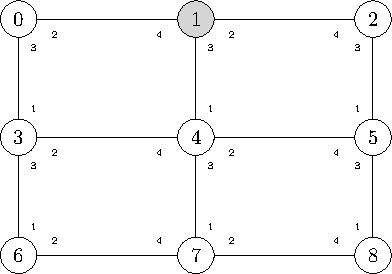
\includegraphics[keepaspectratio,width=0.7\textwidth,height=0.3\textheight]{chapters/nmp/images/3by3gridgraph.pdf}
    \caption[Basic 3×3 grid graph used for the example]{Basic 3×3 grid graph used for the example.  This example will focus on the perspective of node 1.  Other nodes are assumed to work equivalently, but their evolution is not discussed.  Nodes are labelled internally with their ID in the system (\(\iota\) in \cref{fig:nmp:iota_proxels_environment_oracle}), and each intermediary channel with the identity assigned to it by the nearby \gls{pe}.}
    \label{fig:nmp:basicgrid}
\end{figure}

Embodying the unknown processes of the oracle, the data for the received \(v\) terms have been randomly generated for this example and have no particular significance.

To supply a partial demonstration of the expected operation of the rule(s) which would replace the oracle, we compute the contents of outgoing messages according to the following simple rule: \cpruleinline{\cprulenonum{s_4}{\cprecv{\cpvw{W}{G}{\cpfunc{d}{A} \; \cpfunc{d}{B}}}{\iota}}{1}{s_5}{\cpsend{\cpvw{W}{G}{AB}}{\iota}}}  This rule merely sums the data received, and returns the newly computed outgoing message to the relevant node.

\setcounter{traces}{-1}

The total trace for this example is: \tracn{{\label{trace:nmp:0}}--}{--}{--} \tarr{} \tracn{\label{trace:nmp:1}0?*}{0?*}{0?*} \tarr{} \tracn{\label{trace:nmp:2}1?*}{0}{1?} \tarr{} \tracn{\label{trace:nmp:3}1}{0}{2?} \tarr{} \tracn{\label{trace:nmp:4}2?}{1?**}{2} \tarr{} \tracn{\label{trace:nmp:5}2}{2?}{2} \tarr{} \tracn{\label{trace:nmp:6}--}{--}{--}.  Each round number of the trace corresponds to the same row in \cref{tab:nmp:exampleobjects}, reflecting the state of node 1 at the end of that round.  Where the contents of a functor change, the functor and its changed contents are written in boldface to highlight the modifications.

\begin{table}
\setlength\extrarowheight{1ex}
\centering
\begin{tabular}{|l|l|}
\hline
\textbf{Round number} & \textbf{Objects in Node 1} \\ \hline
0 & \(\cpfunc{a}{\cpfunc{n}{2} \, \cpfunc{n}{3} \, \cpfunc{n}{4}}\) \\ \hline
1 & \(\cpfunc{a}{\cpfunc{n}{2} \, \cpfunc{n}{3} \, \cpfunc{n}{4}} \quad \cpfunc{\mathbf{i}}{\mathbf{2}} \quad \cpvvbf{\mathbf{2}}{\mathbf{0}}{\mathbf{1}} \; \cpvvbf{\mathbf{3}}{\mathbf{0}}{\mathbf{4}} \; \cpvvbf{\mathbf{4}}{\mathbf{0}}{\mathbf{7}}\) \\ \hline
2 & \(\cpfunc{a}{\cpfunc{n}{2} \, \cpfunc{n}{3} \, \cpfunc{n}{4}} \quad \cpfunc{i}{2} \quad \cpvvbf{2}{\mathbf{1}}{\mathbf{9}} \; \cpvv{3}{0}{4} \; \cpvvbf{4}{\mathbf{1}}{\mathbf{5}}\)  \\ \hline
3 & \(\cpfunc{a}{\cpfunc{n}{2} \, \cpfunc{n}{3} \, \cpfunc{n}{4}} \quad \cpfunc{i}{2} \quad \cpvv{2}{1}{9} \; \cpvv{3}{0}{4} \; \cpvvbf{4}{\mathbf{2}}{\mathbf{2}}\)  \\ \hline
4 & \(\cpfunc{a}{\cpfunc{n}{2} \, \cpfunc{n}{3} \, \cpfunc{n}{4}} \quad \cpfunc{i}{2} \quad \cpvvbf{2}{\mathbf{2}}{\mathbf{8}} \; \cpvvbf{3}{\mathbf{1}}{\mathbf{3}} \; \cpvv{4}{2}{2}\)  \\ \hline
5 & \(\cpfunc{a}{\cpfunc{n}{2} \, \cpfunc{n}{3} \, \cpfunc{n}{4}} \quad \cpfunc{i}{2} \quad \cpvv{2}{2}{8} \; \cpvvbf{3}{\mathbf{2}}{\mathbf{7}} \; \cpvv{4}{2}{2}\)  \\ \hline
6 & \(\cpfunc{a}{\cpfunc{n}{2} \, \cpfunc{n}{3} \, \cpfunc{n}{4}} \quad \cpfunc{i}{2}\)  \\ \hline
\end{tabular}
\caption[Objects present inside Node 1 at the end of each round]{Objects present inside Node 1 at the end of each round in the example}
\label{tab:nmp:exampleobjects}
\end{table}

\paragraph{Round One}
This round is where node 1 receives its inputs from the environment by rules 1 and 2.  The maximum message generations counter, and the messages with the initial data for the \gls{pe} come through the channel connected to the environment.  Node 1 starts this round holding only its adjacency list, in this case \(\cpfunc{a}{\cpfunc{n}{2} \, \cpfunc{n}{3} \, \cpfunc{n}{4}}\).

The receipt of messages for all three neighbours causes rule 3 to apply and node 1 to enter the sending cycle.  Two new \gls{oq} \(w\) messages are generated relating to each neighbour (because the other two neighbours will take the place of \(Y\) in applications of rule 3a --- recall that there is no \(Z\) in the rule for this node, as it only has three neighbours).  Rule 5 eliminates these duplicates, however, leaving one copy of each message for rule 6 to send to the oracle.  These outgoing messages to the oracle are \(\cpvw{2}{1}{\cpfunc{d}{4} \, \cpfunc{d}{7}}\), \(\cpvw{3}{1}{\cpfunc{d}{1} \, \cpfunc{d}{7}}\) and \(\cpvw{4}{1}{\cpfunc{d}{1} \, \cpfunc{d}{4}}\) for neighbours 2, 3, and 4, respectively.

Node 1 then enters a `blocking wait' (see \cref{sec:cps:blocking}) and remains inactive until the oracle returns the new \gls{nm} messages to send to each neighbour.  Rule 7 sees node 1 receive those messages and then immediately forward them to the neighbours.  The messages are not stored inside node 1 at the end of a step.  Following the example oracle rule described above, the messages sent are \(\cpvv{2}{1}{11}\), \(\cpvv{3}{1}{8}\) and \(\cpvv{4}{1}{5}\) for neighbours 2, 3, and 4, respectively.

The application of rule 7 brings the sending cycle to a close, and node 1 moves to state \(s_5\).  In this state, rule 8 clears away any receipt tokens present in the \gls{pe} and then moves to the termination check of rule 9.  At this point, none of the \(v\) messages hold generation counters equal to the maximum generation count, and so processing will continue.  Finally, node 1 proceeds with another blocking wait, until messages arrive from one or more of its neighbours.

\paragraph{Round Two}
The second round proceeds similarly to the first, but with two key differences.  Firstly, the incoming messages are received from neighbouring \glspl{pe} via the channels connecting node 1 to them.  Secondly, messages are received only from neighbours 2 and 4.  This generates receipt tokens for those neighbours and sees node 1 enter a new sending cycle.

The presence of receipt tokens for both neighbours 2 and 4 leads to the creation of two duplicate \(w\) \gls{oq} messages about neighbour 3.  In effect, 1 and 3 swap roles as \(X\) and \(Y\) in rule 3.  Again, rule 5 eliminates the duplicate, and the single message \(\cpvw{3}{2}{\cpfunc{d}{9} \, \cpfunc{d}{5}}\) is sent to the oracle with rule 6.  In turn, by rule 7, node 1 receives back \(\cpvv{3}{2}{14}\) and forwards it to neighbour 3, completing the sending cycle.  This is also the final message sent to neighbour 3, given that the maximum generation count for this system is two.

As before, node 1 moves from sending to clearing receipt tokens, checking whether it has completed \gls{nm}, and finally becomes quiescent once more, awaiting further messages from neighbours.

\paragraph{Round Three}
Round three begins with receiving a single message, the final message to be received from neighbour 4.  Unlike the earlier rounds, no new messages are sent out due to said receipt.  Neighbour 4 was already one of the neighbours with the highest generation count amongst the messages stored in node 1, and so while it can serve as \(X\) in rule 3, neither of neighbours 2 or 3 can serve as \(Y\) because their generation counts are lower than neighbour 4's.

The fact that rule 3 does \emph{not} apply means that rule 4 \emph{is} applied --- for the first time in this system's evolution.  Rule 4 unconditionally transitions node 1 back to removing all extant receipt tokens, before progressing to the termination check and then returning to awaiting new messages.

\paragraph{Round Four}
This time, neighbour 2 sends its final message, and neighbour 3, at last, sends its first message.  The receipt from neighbour 3 leads to two new single instances of messages relating to neighbours 2 and 4.  The receipt from neighbour 2 could ordinarily lead to another message to be sent to neighbour 3, as it would pair up with neighbour 4 to act as \(X\) and \(Y\), respectively, in rule 3.  This does not occur, however, as neighbour 2 (and 3) has reached the maximum generation count, so rule 3 is no longer applicable for it.

The messages to go to the oracle due to the receipt from neighbour 3 are \(\cpvw{2}{2}{\cpfunc{d}{3} \, \cpfunc{d}{2}}\) and \(\cpvw{4}{2}{\cpfunc{d}{8} \, \cpfunc{d}{3}}\).  Thus, the messages returned by the oracle and sent to neighbour 2 and are \(\cpvv{2}{2}{5}\) and \(\cpvv{4}{2}{11}\).  These are, the last two messages to be sent by node 1 to its neighbours.

\paragraph{Round Five}
Only one more message is still to be received, from neighbour 3 specifically. Node 1 will wait until said message is received, but at that point, all message generation counters will be equal to the maximum, and thus no further messages will be sent out to the neighbours.

Following the application of rule 10 to receive the final message from neighbour 3, node 1 returns to state \(s_2\) and the rules are again explored in top-down order.  This time, rule 3 is inapplicable, so rule 4 is applied, transitioning node 1 to state \(s_5\).  Rule 4 is the only rule applied at this step because it is the only rule which moves from state \(s_2\) to state \(s_5\).  Next, rule 8 deletes the last receipt token.  Again, rule 8 is the only rule applied because it is the only one to feature its state transitions.  Finally, without any \(v\) messages with a generation count below the maximum present in the \gls{pe}, by rule 9, node 1 moves to state \(s_7\) and the finalisation phase.

\paragraph{Round Six}
Round six is the final round of the evolution of the system, for node 1 at least.  With node 1 in state \(s_7\), the only applicable rule is rule 11.  The effect of rule 11 is to send every \(v\) message stored in node 1 to the oracle, renaming them to \(w'\) messages so that the oracle recognises them as finalisation messages rather than \gls{oq} messages for \gls{nm} purposes.

Eventually, the oracle will return the final result message, with the contained datum computed by some means from the messages the oracle received from node 1.  That message is immediately forwarded back to the environment, and evolution of node 1 halts.  Once all other nodes have halted, evolution of the system will have terminated.
\section{\label{sec:nmp:analysis}Asynchronous System Analysis}

This \lcnamecref{sec:nmp:analysis} examines and analyses the asynchronous \gls{pe}-specific system of \cref{sec:nmp:pespecific}.  Firstly, it describes and proves several properties about the system, in particular, that the asynchronous system exchanges precisely the same number of \gls{nm} messages as the \gls{gs} system of \cref{sec:nmp:systemwide}.  Then, it states three conjectures about the system, yet to be proven or disproven mathematically, before examining the asynchronous system's complexity from the standpoint of the rules and symbols used.  Lastly, the \lcnamecref{sec:nmp:analysis} discusses some visualisations of the propagation of ``influence'' from one \gls{pe} in a \gls{fne} grid to others, over multiple steps.

Recall that the fundamental difference in behaviour between the \gls{gs}, \gls{ls} and asynchronous variants is the timing of when they send out new messages relating to when they have received messages for the previous generation.  Under the \gls{gs} approach, \emph{every} \gls{pe} waits until every other \gls{pe} has received all incoming messages before progressing.  Following the \gls{ls} methodology, each \gls{pe} waits until it has received all of its due incoming messages before proceeding, \emph{but without regard} to any other \gls{pe}.  Lastly, for the asynchronous variant, a \gls{pe} waits only until it has received the \(n - 1\) required messages from the other neighbours of generation \(g\) before sending the appropriate generation \(g + 1\) message to the \(n^\text{th}\) neighbour.

\subsection{\label{sec:nmp:msgprops}Messaging Properties and Behaviours}

Consider a cell (\gls{pe}) $\pi_0$ in the asynchronous framework of \cref{sec:nmp:pespecific},
where the maximum generation count is $I$, set by the environment via $\cpfunc{i}{I}$.
Without loss of generality, 
we consider only a \gls{fne} system and
assume that $\pi_0$ is a non-border/non-corner cell with four neighbours, 
$\pi_k$, accessible via channels labelled by $k \in \{ 1, 2, 3, 4 \}$. 

\begin{lemma}\label{lemma:nmp:-0}
    For any $k \in \{ 1, 2, 3, 4 \}$, after each round except the last,
    cell $\pi_0$ contains exactly one $k$-tagged value $\cpvv{k}{\cpdiscard}{\cpdiscard}$, 
    which is accepted from channel $k$ 
    --- except the first round, when that value $v$ comes from the environment channel $e$.
\end{lemma}

\begin{proof}
    By \cpruleref{rule:nmp:proxspec:recvinputs}, cell $\pi_0$ starts by accepting a value $\cpvv{k}{0}{\cpdiscard}$, from the environment channel $e$.
    \cpRuleref{rule:nmp:proxspec:recvfromneighs} gives the only possibility of obtaining another $k$-tagged value, by replacing the current value $v$ with another value $v'$, accepted from channel $k$.
\end{proof}

\begin{remark}
    In fact, \cref{lemma:nmp:-0} holds practically at all times, not just at the end of each round.  The only exceptions are: before the start of the system's evolution and application of \cpruleref{rule:nmp:proxspec:recvinputs}; and after the start of the finalisation phase, specifically after applying \cpruleref{rule:nmp:proxspec:finaloracle}.
\end{remark}

\begin{lemma}\label{lemma:nmp:-1}
    For any $k \in \{ 1, 2, 3, 4 \}$, the time sequence of generation numbers $g \geq 0$ of accepted values $\cpvv{k}{g}{\cpdiscard}$ forms an arithmetic progression with step size one.
\end{lemma}

\begin{proof}
    Proof by induction. Cell $\pi_0$ starts with value $\cpvv{k}{0}{\cpdiscard}$, received via the environment channel $e$.
    Assume that this hypothesis holds for a given $g \geq 0$, appearing as a generation number in value $\cpvv{k}{g}{\cpdiscard}$. \cpRuleref{rule:nmp:proxspec:recvfromneighs} gives the only possibility of changing this number, by replacing the current value with another $v$ value, where the generation number is strictly greater by one, 
    $\cpvv{k}{g+1}{\cpdiscard}$.
\end{proof}

\begin{remark}\label{remark:nmp:-1}
The conclusion of \cref{lemma:nmp:-1} will hold even in the hypothetical case that cell $\pi_k$ would be allowed to send multiple copies of the same message $v$. 
Only the first received copy will be accepted, and the rest will be ignored,
courtesy of \cpruleref{rule:nmp:proxspec:recvfromneighs}. However, this is not the case, as excess \(w\) \gls{oq} messages are deleted by \cpruleref{rule:nmp:proxspec:uniq}. 
\end{remark}

\begin{lemma}\label{lemma:nmp:-2}
    For any $k \in \{ 1, 2, 3, 4 \}$, if channels are reliable and cell $\pi_k$ sends a sequence of messages that reach $\pi_0$ as $\cpvv{k}{g}{\cpdiscard}$, $g \in [1,I]$, 
    then $\pi_0$ accepts all these values in the order of their increasing generation numbers.
\end{lemma}

\begin{proof}
    Channels are reliable, so no message is lost. Channels in \gls{cps} are not inherently FIFO, but cell $\pi_0$ will still pick messages with increasing generation numbers, by \cref{lemma:nmp:-1}.
    As defined by the async version of the model, any messages arriving out-of-order are not lost, but stored in a multiset at the end of the channel
    and will be picked when their time comes.
\end{proof}

\begin{lemma}\label{lemma:nmp:-3}
    For any $k \in \{ 1, 2, 3, 4 \}$, and $g \in [1, I]$: cell $\pi_0$ sends one generation $g$ value $v$ over channel $k$, if and only if $\pi_0$ has received three generation $g-1$ values $v$ from three distinct channels $k' \in 
    \{ 1, 2, 3, 4 \} \setminus \{ k \}$.
\end{lemma}

\begin{proof}
    \textbf{Only if}. Assume that $\pi_0$ sends out a generation $g$ message $v$ over channel $k$.   
    This may only happen by \cpruleref{rule:nmp:proxspec:recvfromoracle}, where $\pi_0$ just forwards the same message $v$, received as $w$ from its oracle. 
    \cpRuleref{rule:nmp:proxspec:sendtooracle} triggers the oracle to build this message $w$, based on three other $v$ messages 
    $\cpvv{k_1}{g_1}{d_1}$, $\cpvv{k_2}{g_2}{d_2}$, $\cpvv{k_3}{g_3}{d_3}$, 
    where $g_1 = g-1$, $g_2, g_3 \geq g_1$, and $k, k_1, k_2, k_3$ are all distinct.
    By \cref{lemma:nmp:-2}, $\pi_0$ must have also received two generation $g-1$ values $v$, from $k_2$ and $k_3$.
    Thus, cell $\pi_0$ has received three values $\cpvv{k_1}{g-1}{d_1}$, $\cpvv{k_2}{g-1}{\cpdiscard}$, $\cpvv{k_3}{g-1}{\cpdiscard}$.
    
    \textbf{If}. Assume that $\pi_0$ accepts three values $\cpvv{k_1}{g'}{d_1}$, $\cpvv{k_2}{g'}{\cpdiscard}$, $\cpvv{k_3}{g'}{\cpdiscard}$, where $g' = g - 1 \geq 0$. These values need not arrive at the same round. Without loss of generality, assume that $\pi_0$ has just received the first value, $\cpvv{k_1}{g'}{d_1}$, while the other values may have been received and even updated already, 
    $\cpvv{k_2}{g'+h_2}{d_2}$, $\cpvv{k_3}{g'+h_3}{d_3}$, $h_2, h_3 \geq 0$.
    \cpRuleref{rule:nmp:proxspec:makews} applies and creates at least two identical \(w\) messages $\cpvw{k_4}{g' + 1}{d}$, where \(d = \cpfunc{d}{d_1}, \, \cpfunc{d}{d_2}, \, \cpfunc{d}{d_3}\). Additional $w$ messages may be created, if either $h_2=0$, or $h_3=0$, or both. This doesn't matter, 
    as excess \(w\) messages are deleted by \cpruleref{rule:nmp:proxspec:uniq}, so only one $\cpvw{k_4}{g' + 1}{d}$ remains.
    This message goes to the oracle, 
    which creates and returns the value $\cpvw{k_4}{g'+1}{d'} = \cpvv{k_4}{g}{d'}$, 
    further forwarded by \cpruleref{rule:nmp:proxspec:recvfromoracle} to $\pi_{k_4}$, over channel $k_4$.
\end{proof}

\begin{remark}
    The behaviour of Lemma~\ref{lemma:nmp:-3} is also true for the \gls{gs} and \gls{ls} variants too.  The key difference for the asynchronous variant is that the new outgoing message for generation \(g\) is sent as soon as possible after those three messages for generation \(g - 1\) have been received, whereas the other two variants will await receipt of the final also message before sending any new ones.
\end{remark}

\begin{theorem}\label{theorem:nmp:-1}
    For each $k \in \{ 1, 2, 3, 4 \}$, and each $g \in [0, I]$:
    \begin{inparaenum}[(i)]
        \item\label{enumitem:nmp:analysis:-1:1} $\pi_0$ receives one $k$-tagged generation $g$ value $v$; and
        \item\label{enumitem:nmp:analysis:-1:2} if $g < I$, $\pi_0$ sends one $k$-tagged generation $g+1$ value $v$.
    \end{inparaenum}
\end{theorem}

\begin{proof}
By bounded induction on $g$. Base case: $g = 0$. By \cpruleref{rule:nmp:proxspec:recvinputs}, cell $\pi_0$ receives \emph{four} $k$-tagged generation $g$ values -- one for each $k \in \{ 1, 2, 3, 4 \}$ -- from the environment channel $e$ (acting on behalf of its neighbour channels). By \cref{lemma:nmp:-3}, applied \emph{four} times, $\pi_0$ sends out \emph{four} generation $g+1$ values $v$, one over each channel $k$.

Induction step: assume that the induction hypothesis holds for 
$g \in [0, I)$, and we prove that it still holds for $g+1$.
The induction hypothesis holds for all cells, 
including $\pi_0$ and $\pi_k$. 
% Thus, by part (ii), each cell $\pi_k$ sends a generation $g+1$ value $v$,
Thus, by part (\ref{enumitem:nmp:analysis:-1:2}), each cell $\pi_k$ sends a generation $g+1$ value $v$, 
which is further received by $\pi_0$, as $\cpvv{k}{g+1}{\cpdiscard}$.
This proves part (\ref{enumitem:nmp:analysis:-1:1}) of the induction step.

If $g+1 < I$, rule 9 does not apply and, 
as shown by \cref{lemma:nmp:-3}, applied \emph{four} times, 
$\pi_0$ sends out \emph{four} generation $g+2$ values $v$, one over each channel $k$.
This proves part (\ref{enumitem:nmp:analysis:-1:2}) of the hypothesis.
\end{proof}

\begin{theorem}\label{theorem:nmp:-2}
    Cell (\gls{pe}) \(\pi_0\) does not send any message to its neighbours at generation \(g > I\).
\end{theorem}

\begin{proof}
    \Gls{oq} \(w\) messages (and thus indirectly \gls{nm} \(v\) messages) are created only by \cpruleref{rule:nmp:proxspec:makews}, with generation counts \(g + 1\), only if \(g + 1 \leq I\).  The promoter \(\cpfunc{i}{G1\cpdiscard}\) for \cpruleref{rule:nmp:proxspec:makews} prevents the creation of any \(w\) message with a larger generation count.
\end{proof}

\begin{theorem}\label{theorem:nmp:-3}
    For each cell $\pi_0$, the neighbourhood (inter-cell) messaging loop stops after receiving the last generation $I$ value.
\end{theorem}

\begin{proof}
    After receiving the last generation \(I\) message, \cpruleref{rule:nmp:proxspec:makews} does not apply (per \cref{theorem:nmp:-2}), and instead control flows by \cpruleref{rule:nmp:proxspec:skiptorecv} to state \(s_5\), then to \(s_6\) by \cpruleref{rule:nmp:proxspec:clearrs}.  Finally, \cpruleref{rule:nmp:proxspec:movetoend} applies, and the control flow breaks out of the main messaging loop, proceeding to state \(s_7\) and the finalisation phase, where no further \gls{nm} occurs. 
\end{proof}

\begin{theorem}\label{theorem:nmp:-4}
    For the asynchronous system in \cref{sec:nmp:pespecific}, 
    each cell (\gls{pe}) sends and receives the same number of messages as in the \gls{gs} system in \cref{sec:nmp:systemwide} and the \gls{ls} system in \cref{sec:nmp:localsync}.   
    Thus, the system as a whole uses the same number of messages.
\end{theorem}

\begin{proof}
    Direct consequence of \cref{theorem:nmp:-1,theorem:nmp:-3}
\end{proof}

\begin{remark}\label{remark:nmp:-2}
    The evolution of the asynchronous version can be suggestively summarised by
    analysing the following four typical cases of cell $\pi_0$ snapshots,
    which focus on the received values having the \emph{least generation number}, here indicated by $g$.
    Note that each star (*) indicates the channel of the incoming value 
    that triggers the sending of a generation $g+1$ message, 
    \emph{not} the channel over which this is sent.
    Without loss of generality, in the case of confluent non-determinism,
    stars are allocated to the first possible choice (for illustrative purposes).
    
    \begin{enumerate}
    \item $(g?***, g?*, g?, g?)$: 
    $\pi_0$ receives all \emph{four} generation $g$ values in the same round, by \cpruleref{rule:nmp:proxspec:recvfromneighs}. 
    As shown by \cref{lemma:nmp:-3}, applied \emph{four} times, 
    $\pi_0$ sends \emph{four} generation $g+1$ values.
    \cpRuleref{rule:nmp:proxspec:makews} will initially create \emph{six} \gls{oq} messages per neighbour (for a total of 24)
    but the excess ones will be deleted, so exactly one \(w\) message per channel will remain and be sent to the oracle.
    
    \medskip
    \item $(g?***, g?*, g?, g_4)$, $g < g_4$: 
    $\pi_0$ receives \emph{three} generation $g$ values in the same round, by \cpruleref{rule:nmp:proxspec:recvfromneighs}.
    The fourth value is at least one generation ahead.    
    This case evolves similarly to case (1) above, with a few changes in the details.
    As shown by \cref{lemma:nmp:-3}, still applied \emph{four} times, 
    $\pi_0$ sends \emph{four} generation $g+1$ values.
    The rules will create \emph{four} \gls{oq} messages for each of the first three channels,
    and \emph{six} \gls{oq} messages for the last channel (for a total of 18),
    but the excess ones will be deleted, so exactly one \gls{oq} message per channel will remain and be sent.
    
    \medskip
    \item $(g?***, g?*, g_3, g_4)$, $g < g_3, g_4$: 
    $\pi_0$ receives \emph{two} generation $g$ values in the same round, by \cpruleref{rule:nmp:proxspec:recvfromneighs}.
    The other two values are at least one generation ahead.    
    This case evolves similarly to case (2) above, with a few changes in the details.
    As shown by \cref{lemma:nmp:-3}, still applied \emph{four} times, 
    $\pi_0$ sends \emph{four} generation $g+1$ values.
    The rules will create \emph{two} \gls{oq} messages for each of the first two channels,
    and \emph{four} \gls{oq} messages for the last two channels (for a total of 12),
    but the excess ones will be deleted, so only one \gls{oq} message per channel will remain and be sent.
    
    \medskip
    \item $(g?***, g_2, g_3, g_4)$, $g < g_2, g_3, g_4$: 
    $\pi_0$ receives \emph{one} single generation $g$ value in a given round, by \cpruleref{rule:nmp:proxspec:recvfromneighs}.
    The last three values are at least one generation ahead.
    As shown by \cref{lemma:nmp:-3}, applied \emph{three} times, 
    $\pi_0$ sends \emph{three} generation $g+1$ values.
    The rules will create and use \emph{two} \gls{oq} messages for each of the last three channels (for a total of 6), but the excess ones will be deleted.
    
    \medskip
    The question arises: when will $\pi_0$ send its fourth generation $g+1$ value, over channel $1$? Brief answer: that message was already sent,
    before the current round!
    
    \medskip
    % Indeed, Lemmas~\ref{lemma:nmp:-1},\ref{lemma:nmp:-2} show that,
    Indeed, \cref{lemma:nmp:-1,lemma:nmp:-2} show that,
    from each channel $k \in \{ 2, 3, 4\}$, 
    $\pi_0$ has received, in order, 
    messages with generation numbers $g, g+1, \ldots, g_k$.
    Consider the round when $\pi_0$ receives the last such message for generation $g$. Without loss of generality, assume that this was from channel $2$.
    Thus, at that round, the summary snapshot was $(g_1, g?, g'_3, g'_4)$,
    with $g_1 < g \leq g'_3, g'_4$.
    By \cref{lemma:nmp:-3}, \emph{one} generation $g+1$ value was then sent over channel $1$.
    \end{enumerate}    
    
    Note also that, at the outset of cases (1,2,3), no other messages for generation $g+1$ will have been sent yet because too few messages at generation $g$ have been received. 
    These notes may be used to create alternate proofs of our main results.

\end{remark}

\subsection{Generational Confluence}
The asynchronous system is \emph{not} (necessarily) confluent.  Messages may be received in such an order that the contents of some messages might not be used in the preparation of new messages, since two messages potentially can be received from one neighbour between receipts from a different neighbour.  Nevertheless, for a \gls{pe} to send a message for generation \(g + 1\) to neighbour \(k\), it must have received messages for \emph{at least} generation \(g\) from all other neighbours.  Therefore, no input data will be `out-of-date'.  This concept is given the name \emph{generational confluence}.

\begin{conjecture}\label{conj:nmp:1}
A \gls{nmp} system following the asynchronous rules of \cref{sec:nmp:pespecific} will be \emph{approximately/generationally} confluent.  Under a wide variety of practical conditions (\eg{} when the base synchronous version is convergent), every evolution of the system will produce a similar result, no matter the specific ordering of the messaging.
\end{conjecture}

\begin{conjecture}\label{conj:nmp:2}
    The asynchronous behaviour, specifically the potential for \glspl{pe} to forgo the use of data from particular messages in favour of newer data, will lead to a final output that is no worse than the synchronous variants' and might result in a `better quality' result, for a particular domain-specific meaning of quality.
\end{conjecture}

Determining the truth or falsity of \cref{conj:nmp:1,conj:nmp:2} is still an open problem requiring further study (but see \cref{sec:nmp:convergence}).  Ideally, one would also clarify and quantify what ``similar'' means in this context.

\begin{proposition}\label{prop:nmp:3}
    No matter the approach to \gls{nmp} employed, the most generations any given \gls{pe} may be ahead of any other \gls{pe} on the lattice depends on their distance from each other, as measured by the smallest number of intermediate \glspl{pe} along any path between the two.
\end{proposition}

The requirement for a \gls{pe} to have received messages from every other neighbour before preparing a message to send to the final neighbour means that, at a certain point, a \gls{pe} transitively depends on its neighbours' neighbours in an ever-expanding radius.  A given \gls{pe} cannot send a new message to neighbour 4 until it has received messages from neighbours 1-3.  In turn, neighbour 4 cannot send messages to any of its other neighbours besides the original \gls{pe} until it has received the next message from the original \gls{pe}.  The same then applies to those neighbours of the original \gls{pe}'s neighbour 4, \etc{}.

This reasoning gives rise to the intuition in \cref{prop:nmp:3}.  If one of the \glspl{pe} stops sending messages but has not yet reached its maximum generation, the neighbouring \glspl{pe} will successively be unable to send further messages themselves, which will ripple across the lattice and eventually prevent farther \glspl{pe} from sending further messages as well.  Until the ripple has progressed across the lattice, however, the more remote \glspl{pe} may still send new messages.  Therefore, in all cases where two \glspl{pe} have a path between them, there is an inter-dependency, albeit in some cases far removed.  As yet, no suitable and convincing formal proof of this idea has been found.

\subsection{Rule and Symbol Complexity}
Overall, the rule and symbol complexity of the system is relatively low, but given that some elements of any specific \gls{nmp} process are abstracted away (\eg{} the oracle), this is likely an underestimate for a given final implementation.

\subsubsection{Rule Complexity}
The total system requires 12 rules.  Two for the initialisation phase, eight for the joint \gls{nm} \& \gls{oq} phases -- only two directly involve interaction with the oracle, but others prepare for said interaction -- and two for the finalisation phase.  The two rules that involve direct interaction with the oracle, rules \cpruleref*{rule:nmp:proxspec:sendtooracle} and \cpruleref*{rule:nmp:proxspec:recvfromoracle}, will normally be replaced with an arbitrary new \gls{ruleset}, however.  Thus, it can be said that there are 10 rules relating to the structure and process for \gls{nmp}, and two stub rules which stand in for a more complex process.

\subsubsection{Symbol Complexity}
Across all 12 rules, three atoms, eight functors, and nine states are used.  This gives a total symbol complexity of 20 distinct symbols.  As with the rule complexity, there likely will be more symbols used when the \gls{oq} phase is expanded to encompass a desired computation process.

\subsection{Visualisations}
Sequences of visualisations of the evolution of a sample \gls{fne} system have been created to explore the messaging behaviour of \gls{nmp}.  These sequences reflect the changes on a small grid that result from \gls{nmp} following \cref{sec:nmp:pespecific}'s system.  Each square on a grid represents one \gls{pe}, and the \glspl{pe} are assumed to be connected in the standard \gls{fne} manner.

Each sequence was generated using a script by computing values over the grid at the end of each round of messaging and writing the results out to a standalone .tex file, then compiling the .tex file to produce an output .pdf.  In each case, the grid starts with all zero values, except for the centre \gls{pe}, which starts with a `full-strength' value --- represented by wholly white and completely black squares, respectively.  The value to display at a given grid point for each round was in turn computed by selecting the maximum from among the data stored in the corresponding \gls{pe}.

Each of the sequences uses a different method for computing the values present in a given square, and so depicts a different aspect of the spread of the `influence' of the initial data in the centre \gls{pe}.  The approach used here was effectively the \gls{ls} variant, but the results apply equally to the variants.

\subsubsection{Maximum Over Messages Received and Internal Datum}
\begin{figure}
    \centering
    \subcaptionbox{Round 0}{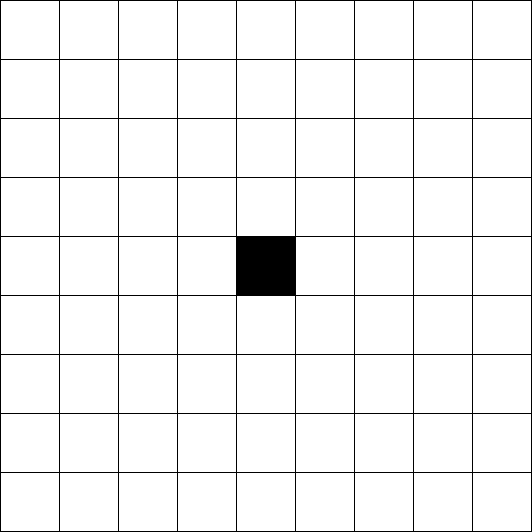
\includegraphics[width=0.19\textwidth]{chapters/nmp/images/grids/maxpdatum/nodelay/maxWithPDatum_no_delays_four_generations_round_0.pdf}}
    \subcaptionbox{Round 1}{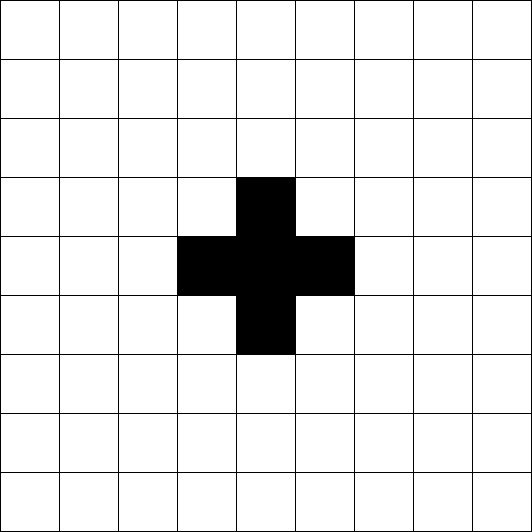
\includegraphics[width=0.19\textwidth]{chapters/nmp/images/grids/maxpdatum/nodelay/maxWithPDatum_no_delays_four_generations_round_1.pdf}}
    \subcaptionbox{Round 2}{
\includegraphics[width=0.19\textwidth]{chapters/nmp/images/grids/maxpdatum/nodelay/maxWithPDatum_no_delays_four_generations_round_2.pdf}}
    \subcaptionbox{Round 3}{
\includegraphics[width=0.19\textwidth]{chapters/nmp/images/grids/maxpdatum/nodelay/maxWithPDatum_no_delays_four_generations_round_3.pdf}}
    \subcaptionbox{Round 4}{
\includegraphics[width=0.19\textwidth]{chapters/nmp/images/grids/maxpdatum/nodelay/maxWithPDatum_no_delays_four_generations_round_4.pdf}}
    \caption[Visualisation of the spread of `influence' from the centre \glsxtrshort{pe} during \glsxtrlong{nmp}]{Visualisation of the spread of `influence' from the centre \gls{pe} during \gls{nmp}.  Each square's value was computed as the maximum over both the last messages received, and a datum stored by the \gls{pe}}
    \label{fig:nmp:maxpdatum}
\end{figure}

The sequence in \cref{fig:nmp:maxpdatum} was produced by using the maximum of the \gls{pe}'s current messages received from the other neighbours \emph{and} a separate value stored internally and updated when computing the new outgoing messages.  The extra value was updated at each step to be the maximum of itself or the messages currently held.  The net effect of this was to ensure that when a message carrying information from the centre \gls{pe} arrived, the current \gls{pe} would turn black and remain that way.  \Cref{fig:nmp:maxpdatum} shows that this information propagates outwards as expected, given the nature of the updates.

\begin{figure}
    \centering
    \subcaptionbox{Round 0}{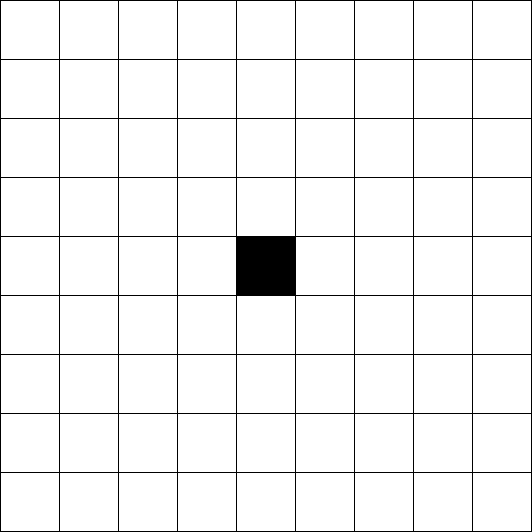
\includegraphics[width=0.19\textwidth]{chapters/nmp/images/grids/maxpdatum/delay2/maxWithPDatum_delay2_four_generations_round_0.pdf}}
    \subcaptionbox{Round 1}{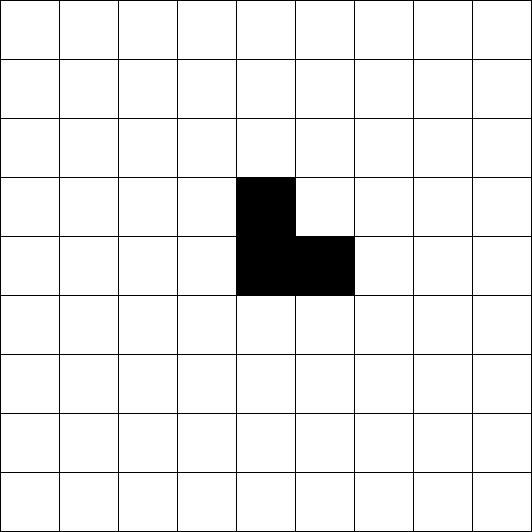
\includegraphics[width=0.19\textwidth]{chapters/nmp/images/grids/maxpdatum/delay2/maxWithPDatum_delay2_four_generations_round_1.pdf}}
    \subcaptionbox{Round 2}{\includegraphics[width=0.19\textwidth]{chapters/nmp/images/grids/maxpdatum/delay2/maxWithPDatum_delay2_four_generations_round_2.pdf}}
    \subcaptionbox{Round 3}{\includegraphics[width=0.19\textwidth]{chapters/nmp/images/grids/maxpdatum/delay2/maxWithPDatum_delay2_four_generations_round_3.pdf}}
    \subcaptionbox{Round 4}{\includegraphics[width=0.19\textwidth]{chapters/nmp/images/grids/maxpdatum/delay2/maxWithPDatum_delay2_four_generations_round_4.pdf}}
    \subcaptionbox{Round 5}{\includegraphics[width=0.19\textwidth]{chapters/nmp/images/grids/maxpdatum/delay2/maxWithPDatum_delay2_four_generations_round_5.pdf}}
    \subcaptionbox{Round 6}{\includegraphics[width=0.19\textwidth]{chapters/nmp/images/grids/maxpdatum/delay2/maxWithPDatum_delay2_four_generations_round_6.pdf}}
    \subcaptionbox{Round 7}{\includegraphics[width=0.19\textwidth]{chapters/nmp/images/grids/maxpdatum/delay2/maxWithPDatum_delay2_four_generations_round_7.pdf}}
    \subcaptionbox{Round 8}{\includegraphics[width=0.19\textwidth]{chapters/nmp/images/grids/maxpdatum/delay2/maxWithPDatum_delay2_four_generations_round_8.pdf}}
    \subcaptionbox{Round 9}{\includegraphics[width=0.19\textwidth]{chapters/nmp/images/grids/maxpdatum/delay2/maxWithPDatum_delay2_four_generations_round_9.pdf}}
    \caption[Visualisation of the spread of `influence' from the centre \glsxtrshort{pe} during \glsxtrlong{nmp}]{Visualisation of the spread of `influence' from the centre \gls{pe} during \gls{nmp}.  Each square's value was computed as the maximum over both the last messages received, and a datum stored by the \gls{pe}, and with delivery delays of two rounds on messages going to the neighbours below and to the left}
    \label{fig:nmp:maxpdatumdelays}
\end{figure}

More interesting is \cref{fig:nmp:maxpdatumdelays}.  The same update computations were performed, but a two-round delay was introduced for the delivery of messages to the neighbours below and to the left of the sending \gls{pe}.  Messages destined for the neighbours to the right and above of the sending \gls{pe} were delivered without delays, as in \cref{fig:nmp:maxpdatum}.  The eventual symmetry of the shape may seem surprising at first, but is actually logical.  Remember that every \gls{pe}/square on the grid is a neighbour of the ones to the top and right, and will only receive messages from those neighbours after the two-round delay --- which consequently means that they in turn only send out messages to their bottom and left \emph{after} that delay.  See also \cref{prop:nmp:3}.

What might happen if there is a systematic delay in only one direction, and thus potentially messages from all other neighbours might arrive relatively quickly?  This is examined in \cref{fig:nmp:maxpdatumdelayswestonly}, where a two round delay was introduced for messages sent to the left only.  In this case, the overall shape of the \glspl{pe} on the grid who have received a message containing `influence' from the centre \gls{pe} still invariably ends up returning to a symmetrical, balanced shape.  It is a different shape, however, from that seen in \cref{fig:nmp:maxpdatum,fig:nmp:maxpdatumdelays}, and is not centred on the centre \gls{pe}.  Instead, it grows with a bias towards the right.%  This eventual symmetry may appear surprising at first, but is to be expected for similar reasons to the basis for \autoref{prop:3}.  A \gls{pe} can only send a message to a neighbour once it has received the messages from the other neighbours, and this dependency is (effectively) transitive.  Thus, if some messages take much longer to arrive, \glspl{pe} will end up being forced to wait for them, directly or indirectly.

\begin{figure}
    \centering
    \subcaptionbox{Round 0}{\includegraphics[width=0.19\textwidth]{chapters/nmp/images/grids/maxpdatum/delay2westonly/maxWithPDatum_delay2_west_only_four_generations_round_0.pdf}}
    \subcaptionbox{Round 1}{\includegraphics[width=0.19\textwidth]{chapters/nmp/images/grids/maxpdatum/delay2westonly/maxWithPDatum_delay2_west_only_four_generations_round_1.pdf}}
    \subcaptionbox{Round 2}{\includegraphics[width=0.19\textwidth]{chapters/nmp/images/grids/maxpdatum/delay2westonly/maxWithPDatum_delay2_west_only_four_generations_round_2.pdf}}
    \subcaptionbox{Round 3}{\includegraphics[width=0.19\textwidth]{chapters/nmp/images/grids/maxpdatum/delay2westonly/maxWithPDatum_delay2_west_only_four_generations_round_3.pdf}}
    \subcaptionbox{Round 4}{\includegraphics[width=0.19\textwidth]{chapters/nmp/images/grids/maxpdatum/delay2westonly/maxWithPDatum_delay2_west_only_four_generations_round_4.pdf}}
    \subcaptionbox{Round 5}{\includegraphics[width=0.19\textwidth]{chapters/nmp/images/grids/maxpdatum/delay2westonly/maxWithPDatum_delay2_west_only_four_generations_round_5.pdf}}
    \subcaptionbox{Round 6}{\includegraphics[width=0.19\textwidth]{chapters/nmp/images/grids/maxpdatum/delay2westonly/maxWithPDatum_delay2_west_only_four_generations_round_6.pdf}}
    \subcaptionbox{Round 7}{\includegraphics[width=0.19\textwidth]{chapters/nmp/images/grids/maxpdatum/delay2westonly/maxWithPDatum_delay2_west_only_four_generations_round_7.pdf}}
    \subcaptionbox{Round 8}{\includegraphics[width=0.19\textwidth]{chapters/nmp/images/grids/maxpdatum/delay2westonly/maxWithPDatum_delay2_west_only_four_generations_round_8.pdf}}
    \subcaptionbox{Round 9}{\includegraphics[width=0.19\textwidth]{chapters/nmp/images/grids/maxpdatum/delay2westonly/maxWithPDatum_delay2_west_only_four_generations_round_9.pdf}}
    \caption[Visualisation of the spread of `influence' from the centre \glsxtrshort{pe} during \glsxtrlong{nmp}.]{Visualisation of the spread of `influence' from the centre \gls{pe} during \gls{nmp}.  Each square's value was computed as the maximum over both the last messages received, and a datum stored by the \gls{pe}, and with delivery delays of two rounds on messages going to the left only}
    \label{fig:nmp:maxpdatumdelayswestonly}
\end{figure}

\subsubsection{Maximum Over Messages Received}
\begin{figure}
    \centering
    \subcaptionbox{Round 0}{\includegraphics[width=0.19\textwidth]{chapters/nmp/images/grids/max/nodelay/max_no_delay_four_generations_round_0.pdf}}
    \subcaptionbox{Round 1}{\includegraphics[width=0.19\textwidth]{chapters/nmp/images/grids/max/nodelay/max_no_delay_four_generations_round_1.pdf}}
    \subcaptionbox{Round 2}{\includegraphics[width=0.19\textwidth]{chapters/nmp/images/grids/max/nodelay/max_no_delay_four_generations_round_2.pdf}}
    \subcaptionbox{Round 3}{\includegraphics[width=0.19\textwidth]{chapters/nmp/images/grids/max/nodelay/max_no_delay_four_generations_round_3.pdf}}
    \subcaptionbox{Round 4}{\includegraphics[width=0.19\textwidth]{chapters/nmp/images/grids/max/nodelay/max_no_delay_four_generations_round_4.pdf}}
    \caption[Visualisation of the spread of `influence' from the centre \glsxtrshort{pe} during \glsxtrlong{nmp}]{Visualisation of the spread of `influence' from the centre \gls{pe} during \gls{nmp}.  Each square's value was computed as the maximum over the last messages received}
    \label{fig:nmp:max}
\end{figure}

The sequence in \cref{fig:nmp:max} was produced by using the maximum of the messages received from the other neighbours when computing the new outgoing messages for each \gls{pe}.\footnote{Given that both systems only have two values for each cell and updates to a given cell are based on values in surrounding ones, it does not seem coincidental that this progression bears some resemblance to Conway's Game of Life.}  As with the sequence in \cref{fig:nmp:maxpdatum}, the spread of the influence from the centre \gls{pe} moves outward, similar to an expanding `+' shape.  Notably, however, points in the grid (except the centre \gls{pe} for one round) oscillate between the minimum and the maximum, showing that the influence from the centre \gls{pe} is only relevant for every second message update computation.  Felzenzswalb \& Huttenlocher \cite{Felzenszwalb2006} noticed this oscillating behaviour and used it to halve the number of computations required to produce the same results in their improved \gls{bp} \gls{sm} implementation.

\subsubsection{Mean Over Messages Received}
\begin{figure}
    \centering
    \subcaptionbox{Round 0}{\includegraphics[width=0.19\textwidth]{chapters/nmp/images/grids/mean/nodelay/mean_no_delay_four_generations_round_0.pdf}}
    \subcaptionbox{Round 1}{\includegraphics[width=0.19\textwidth]{chapters/nmp/images/grids/mean/nodelay/mean_no_delay_four_generations_round_1.pdf}}
    \subcaptionbox{Round 2}{\includegraphics[width=0.19\textwidth]{chapters/nmp/images/grids/mean/nodelay/mean_no_delay_four_generations_round_2.pdf}}
    \subcaptionbox{Round 3}{\includegraphics[width=0.19\textwidth]{chapters/nmp/images/grids/mean/nodelay/mean_no_delay_four_generations_round_3.pdf}}
    \subcaptionbox{Round 4}{\includegraphics[width=0.19\textwidth]{chapters/nmp/images/grids/mean/nodelay/mean_no_delay_four_generations_round_4.pdf}}
    \caption[Visualisation of the spread of `influence' from the centre \glsxtrshort{pe} during \glsxtrlong{nmp}]{Visualisation of the spread of `influence' from the centre \gls{pe} during \gls{nmp}.  Each square's value was computed as the mean over the last messages received}
    \label{fig:nmp:mean}
\end{figure}

The sequence in \cref{fig:nmp:mean} was produced by using the mean of the messages received from the other neighbours when computing the new outgoing messages for each \gls{pe}.  This sequence makes it clear that as the initial information from a given \gls{pe} diffuses across the grid, its direct influence upon the data in the \glspl{pe} gradually dilutes.  After just four rounds of message passing, the `signal strength' from the centre \gls{pe} has become so weak as to be almost imperceptible in the most distant locations it has reached, \eg{} points (0,4) and (4,8), assuming a zero-based grid count beginning in the upper-left corner.
\section{\label{sec:nmp:experiments}Experimental Results}

This \namecref{sec:nmp:experiments} presents the results of a handful of small experiments with short prototype programs, performed to validate \cref{ruleset:nmp:proxspec} and investigate the properties of the \gls{pe}-specific approach to \gls{nmp}.  In particular, these experiments:
\begin{inparaenum}[(i)]
\item simulated the operation of the \gls{ruleset} without actually passing messages, to verify empirically that \cref{theorem:nmp:-4} holds for an arbitrary \gls{pe};
\item implemented and benchmarked three variants of the three \gls{nmp} variants operating on a \gls{fne} grid, to assess whether the fully asynchronous version genuinely completes faster on average;
\item investigated the variants' convergence behaviour;
\item compared the timings of the variants for when the first, `average' and last \gls{pe} finish their processing.
\end{inparaenum}
Source code for the described scripts or programs may be found at \url{https://github.com/jcoo092/NeighbourhoodMessagePassingExperiments}.

\subsection{Validation of Rules for Asynchronous Neighbourhood Message Passing}
A short script was written in \fsharp{}.  This script takes the perspective of a single arbitrary \gls{pe} on a \gls{fne} grid and simulates the receipt and sending of messages.  Actual data are irrelevant to this test, so message data \gls{oq} updates were omitted.  During each round, the \gls{pe} `receives messages' from one or more randomly selected neighbours.  Said receipts are represented by incrementing the received-message generation counts and creating receipt tokens.  The \gls{pe} then generates \gls{nm} messages per \cref{ruleset:nmp:proxspec} based on the generation counts and receipt tokens, and increments the sent-message counts as appropriate.  The script prints the results, then terminates once messaging completes.

Inspecting the state of the \gls{pe} at various points in the system's execution strongly supported \cref{theorem:nmp:-4}.  If exactly \(g\) messages were received from each neighbour, where \(g\) is the maximum generation count, the same number of messages would consequently be sent.  Furthermore, messages were indeed sent based on the ordering of messages received, as expected.

\subsection{\label{sec:nmp:timingexp}Timing of Variations}
A self-contained command-line program was written in C\# to investigate the comparative running time of each of the three variants described above using the \gls{fne} grid.  Each \gls{pe} is represented by a separate asynchronous \texttt{Task} from .NET's Task Parallel Library{\footnote{\raggedright\url{https://docs.microsoft.com/en-us/dotnet/standard/parallel-programming/task-parallel-library-tpl}}}, with communication between \glspl{pe} conducted via a channel construct provided by .NET.\footnote{\url{https://docs.microsoft.com/en-us/dotnet/api/system.threading.channels}}  All three approaches are included in the same program, and selected via a configuration file supplied at runtime. The use of \texttt{Task}s, which the .NET runtime schedules to work in parallel when possible, means that all three variants are expected to run faster on a CPU with more cores.   More \glspl{pe} can execute physically (as opposed to logically) simultaneously on the larger CPU, so while total CPU time might stay constant, ``wall clock'' time should reduce.

Multiple variables besides the variant were used over different runs to explore the relative behaviour of each variant in terms of running time.  These included:
\begin{inparablank}
\item the size of the grid;
\item the maximum generation count;
\item the use and length of a work-intensive wait period when computing a new message to send (essentially, the \gls{oq} phase);
\item the use and length of delays in delivery of messages over the channels while permitting the \glspl{pe} to continue operating;
\item as well as using different delay lengths for different directions.
\end{inparablank}

Running time results were gathered using the \texttt{Stopwatch} class from .NET, which provides access to underlying high-performance operating system time measurement facilities.  The program is instrumented to start the timer immediately before the initialisation of the \glspl{pe}, but \emph{after} reading and parsing the configuration file.  The timer is then stopped immediately after the last \gls{pe} finishes running, when control flow returns to the program's \texttt{main} function.  The total elapsed milliseconds are then printed to the command line.  Numerical results are presented in \crefrange{tab:nmp:simulation8cores}{tab:nmp:simulation48cores}.  The numbers presented in the tables are the mean (rounded to the nearest whole number) of five runs for each variant under each parameter set.

Early testing showed that there was no meaningful difference between variants
regarding generation count, so in all instances the results are from running the program with a maximum generation count of \num{20} and an oracle delay of approximately one-quarter of a millisecond per message.  The delays over channels were varied between equal delays of \qty{30}{\milli\second}, three channels with \qty{30}{\milli\second} and one with \qty{150}{\milli\second}, and two channels with \qty{30}{\milli\second} and two with \qty{150}{\milli\second}.  The test program was run on three different computers with three different CPUs, each with a different number of physical \& logical cores.  The CPUs were an Intel\textsuperscript{\textregistered} Core\textsuperscript{\texttrademark} i7-7700, with 4 physical/8 logical cores; an Intel\textsuperscript{\textregistered} Core\textsuperscript{\texttrademark} i7-8750H with 6 physical/12 logical cores; and an Intel\textsuperscript{\textregistered} Xeon\textsuperscript{\textregistered} Silver 4116 with 24 physical/48 logical cores.

\begin{table}
\centering
\resizebox{\textwidth}{!}{%
\begin{tabular}{@{}r|rrr|rrr|rrr@{}}
\toprule
\multicolumn{1}{c|}{\# of}   & \multicolumn{3}{c|}{Equal delays} & \multicolumn{3}{c|}{One longer delay} & \multicolumn{3}{c}{Two longer delays} \\ \cmidrule(l){2-10} 
\multicolumn{1}{c|}{Proxels} & Global    & Local     & Async     & Global      & Local      & Async      & Global      & Local      & Async      \\ \midrule
\num{361}  & \num{1 553}  & \num{1 212}  & \num{1 212}  & \num{4 029}  & \num{3 226}  & \num{3 104}  & \num{4 026}  & \num{3 514}  & \num{3 516}  \\
\num{9 801}  & \num{21 012}  & \num{20 442}  & \num{18 865}  & \num{25 976}  & \num{23 281}  & \num{21 311}  & \num{24 282}  & \num{21 410}  & \num{19 679}  \\
\num{89 401}  & \num{192 730}  & \num{192 329}  & \num{174 984}  & \num{225 454}  & \num{219 261}  & \num{200 889}  & \num{222 104}  & \num{216 537}  & \num{200 637}  \\
\num{249 001}  & \num{542 285}  & \num{546 213}  & \num{493 311}  & \num{625 959}  & \num{595 861}  & \num{527 898}  & \num{614 079}  & \num{564 406}  & \num{558 970} \\ \bottomrule
\end{tabular}%
}
\caption[Mean recorded running times for each \glsxtrlong{nmp} variant on an 8-core CPU]{Mean recorded running times in milliseconds for each \gls{nmp} variant in a simulation, with different sending delay lengths, on a computer with a CPU with 4/8 physical/logical cores}
\label{tab:nmp:simulation8cores}
\end{table}

\begin{table}
\centering
\resizebox{\textwidth}{!}{%
\begin{tabular}{@{}r|rrr|rrr|rrr@{}}
\toprule
\multicolumn{1}{c|}{\# of}   & \multicolumn{3}{c|}{Equal delays} & \multicolumn{3}{c|}{One longer delay} & \multicolumn{3}{c}{Two longer delays} \\ \cmidrule(l){2-10} 
\multicolumn{1}{c|}{Proxels} & Global    & Local     & Async     & Global      & Local      & Async      & Global      & Local      & Async      \\ \midrule
\num{361}  & \num{1 457}  & \num{1 186}  & \num{1 148}  & \num{3 875}  & \num{3 229}  & \num{3 096}  & \num{3 918}  & \num{3 471}  & \num{3 493}  \\
\num{9 801}  & \num{15 865}  & \num{15 116}  & \num{14 290}  & \num{18 392}  & \num{15 295}  & \num{14 564}  & \num{18 389}  & \num{15 267}  & \num{14 612}  \\
\num{89 401}  & \num{145 547}  & \num{141 024}  & \num{133 509}  & \num{149 368}  & \num{141 811}  & \num{134 382}  & \num{148 439}  & \num{141 619}  & \num{134 289}  \\
\num{249 001}  & \num{408 463}  & \num{392 901}  & \num{371 576}  & \num{413 106}  & \num{391 907}  & \num{370 683}  & \num{413 224}  & \num{394 115}  & \num{372 556} \\ \bottomrule
\end{tabular}%
}
\caption[Mean recorded running times for each \glsxtrlong{nmp} variant on a 12-core CPU]{Mean recorded running times in milliseconds for each \gls{nmp} variant in a simulation, with different sending delay lengths, on a computer with a CPU with 6/12 physical/logical cores}
\label{tab:nmp:simulation12cores}
\end{table}

\begin{table}
\centering
\resizebox{\textwidth}{!}{%
\begin{tabular}{@{}r|rrr|rrr|rrr@{}}
\toprule
\multicolumn{1}{c|}{\# of}   & \multicolumn{3}{c|}{Equal delays} & \multicolumn{3}{c|}{One longer delay} & \multicolumn{3}{c}{Two longer delays} \\ \cmidrule(l){2-10} 
\multicolumn{1}{c|}{Proxels} & Global    & Local     & Async     & Global      & Local      & Async      & Global      & Local      & Async      \\ \midrule
\num{361}  & \num{1 370}  & \num{1 248}  & \num{1 122}  & \num{3 710}  & \num{3 204}  & \num{3 091}  & \num{3 741}  & \num{3 436}  & \num{3 419}  \\
\num{9 801}  & \num{9 986}  & \num{9 060}  & \num{7 571}  & \num{12 012}  & \num{9 549}  & \num{8 007}  & \num{11 932}  & \num{9 392}  & \num{7 911}  \\
\num{89 401}  & \num{102 718}  & \num{92 817}  & \num{76 583}  & \num{106 166}  & \num{96 293}  & \num{78 341}  & \num{106 984}  & \num{94 060}  & \num{78 025}  \\
\num{249 001}  & \num{296 516}  & \num{255 703}  & \num{215 504}  & \num{299 926}  & \num{265 365}  & \num{215 721}  & \num{298 732}  & \num{263 814}  & \num{216 048} \\ \bottomrule
\end{tabular}%
}
\caption[Mean recorded running times for each \glsxtrlong{nmp} variant on a 48-core CPU]{Mean recorded running times in milliseconds for each \gls{nmp} variant in a simulation, with different sending delay lengths, on a computer with a CPU with 24/48 physical/logical cores}
\label{tab:nmp:simulation48cores}
\end{table}

The data from \crefrange{tab:nmp:simulation8cores}{tab:nmp:simulation48cores} are visualised in \crefrange{fig:nmp:timings8cores}{fig:nmp:timings48cores}, with the variants on the x-axis and milliseconds on the y-axis.  Each figure has four bar charts for the four different grid sizes used, which were \numproduct{19 x 19}, \numproduct{99 x 99}, \numproduct{299 x 299} and \numproduct{499 x 499}, giving total \gls{pe} counts of \num{361}, \num{9 801}, \num{89 401} and \num{249 001} \glspl{pe}, respectively.  Each chart compares the \gls{gs}, \gls{ls} and asynchronous variants, both against each other and between the different numbers of longer channel delays used.  In every figure, the chart layout for the grid sizes (in number of \glspl{pe}) is as follows:
\begin{inparablank}
\item top-right, \num{361};
\item top-left, \num{9 801};
\item bottom-left, \num{89 401};
\item bottom-right, \num{249 001}.
\end{inparablank}
In each chart, the bar clusters are the timings for, from left to right:
\begin{inparaenum}[a)]
\item the experiments when there were equal delays on all channels;
\item the experiments when there was a longer delay on one channel;
\item and the experiments where there were longer delays on two channels.
\end{inparaenum}
Within each bar cluster, in every instance, the bars represent the timings for (from left to right):  the \gls{gs}, \gls{ls} and asynchronous variants.  The y-axes \emph{do not} follow the same scale, however.

\begin{figure}
    \centering
    \begin{tikzpicture}
        \begin{groupplot}[ %361 proxels
            group style={
                group size=2 by 2,
                vertical sep=0.70cm,
                xlabels at=edge bottom,
                xticklabels at=edge bottom,
                ylabels at=edge left,
            },
            enlargelimits=0.25,
            height=0.50\textheight,
            symbolic x coords={Equal,One,Two},
            small,
            width=0.52\textwidth,
            xlabel=Number of longer delays,
            xtick={data},
            ybar,
            ylabel=Milliseconds,
        ]
            % 361
            \nextgroupplot
            \addplot %global
            coordinates {
                (Equal,1553) (One,4029) (Two,4026)   
            };
            \addplot %local
            coordinates {
                (Equal,1212) (One,3226) (Two,3514)   
            };
            \addplot %async
            coordinates {
                (Equal,1212) (One,3104) (Two,3516)   
            };
            
            % \num{9 801}
            \nextgroupplot
            \addplot %global
            coordinates {
                (Equal,21012) (One,25976) (Two,24282)   
            };
            \addplot %local
            coordinates {
                (Equal,20442) (One,23281) (Two,21410)   
            };
            \addplot %async
            coordinates {
                (Equal,18865) (One,21311) (Two,19679)   
            };
            
            % \num{89 401}
            \nextgroupplot
            \addplot %global
            coordinates {
                (Equal,192730) (One,225454) (Two,222104)   
            };
            \addplot %local
            coordinates {
                (Equal,192329) (One,219261) (Two,216537)   
            };
            \addplot %async
            coordinates {
                (Equal,174984) (One,200889) (Two,200637)   
            };
            
            % \num{249 001}
            \nextgroupplot
            \addplot %global
            coordinates {
                (Equal,542285) (One,625959) (Two,614079)   
            };
            \addplot %local
            coordinates {
                (Equal,546213) (One,595861) (Two,564406)   
            };
            \addplot %async
            coordinates {
                (Equal,493311) (One,527898) (Two,558970)   
            };
        \end{groupplot}
    \end{tikzpicture}
    \caption[Bar chart visualising the timing differences for the variants on an 8-core CPU]{Bar chart visualising the timing differences for the variants running on a CPU with 8 cores, with different sized grids and differing channel delay lengths.  Each bar cluster goes from left to right with the \gls{gs}, \gls{ls} and asynchronous variants, respectively.  The numbers of \glspl{pe} are:  Top-left: 361;  Top-right:  \num{9 801};  Bottom-left:  \num{89 401};  Bottom-right:  \num{249 001}.  See also \cref{tab:nmp:simulation8cores}}
    \label{fig:nmp:timings8cores}
\end{figure}

\begin{figure}
    \centering
    \begin{tikzpicture}
        \begin{groupplot}[
            group style={
                group size=2 by 2,
                vertical sep=0.70cm,
                xlabels at=edge bottom,
                xticklabels at=edge bottom,
                ylabels at=edge left,
            },
            enlargelimits=0.25,
            height=0.50\textheight,
            symbolic x coords={Equal,One,Two},
            small,
            width=0.52\textwidth,
            xlabel=Number of longer delays,
            xtick={data},
            ybar,
            ylabel=Milliseconds,
        ]
            % 361
            \nextgroupplot
            \addplot %global
            coordinates {
                (Equal,1457) (One,3875) (Two,3918)   
            };
            \addplot %local
            coordinates {
                (Equal,1186) (One,3229) (Two,3471)   
            };
            \addplot %async
            coordinates {
                (Equal,1148) (One,3096) (Two,3493)   
            };
            
            % \num{9 801}
            \nextgroupplot
            \addplot %global
            coordinates {
                (Equal,15865) (One,18392) (Two,18389)   
            };
            \addplot %local
            coordinates {
                (Equal,15116) (One,15295) (Two,15267)   
            };
            \addplot %async
            coordinates {
                (Equal,14290) (One,14564) (Two,14612)   
            };
            
            % \num{89 401}
            \nextgroupplot
            \addplot %global
            coordinates {
                (Equal,145547) (One,149368) (Two,148439)   
            };
            \addplot %local
            coordinates {
                (Equal,141024) (One,141811) (Two,141619)   
            };
            \addplot %async
            coordinates {
                (Equal,133509) (One,134382) (Two,134289)   
            };
            
            % \num{249 001}
            \nextgroupplot
            \addplot %global
            coordinates {
                (Equal,408463) (One,413106) (Two,413224)   
            };
            \addplot %local
            coordinates {
                (Equal,392901) (One,391907) (Two,394115)   
            };
            \addplot %async
            coordinates {
                (Equal,371576) (One,370683) (Two,372556)   
            };
        \end{groupplot}
    \end{tikzpicture}
    \caption[Bar chart visualising the timing differences for the variants on a 12-core CPU]{Bar chart visualising the timing differences for the variants running on a CPU with 12 cores, with different sized grids and differing channel delay lengths.  Each bar cluster goes from left to right with the \gls{gs}, \gls{ls} and asynchronous variants, respectively.  The numbers of \glspl{pe} are:  Top-left: 361;  Top-right:  \num{9 801};  Bottom-left:  \num{89 401};  Bottom-right:  \num{249 001}.  See also \cref{tab:nmp:simulation12cores}}
    \label{fig:nmp:timings12cores}
\end{figure}

\begin{figure}
    \centering
    \begin{tikzpicture}
        \begin{groupplot}[ %361 proxels
            group style={
                group size=2 by 2,
                vertical sep=0.70cm,
                xlabels at=edge bottom,
                xticklabels at=edge bottom,
                ylabels at=edge left,
            },
            enlargelimits=0.25,
            height=0.50\textheight,
            symbolic x coords={Equal,One,Two},
            small,
            width=0.52\textwidth,
            xlabel=Number of longer delays,
            xtick={data},
            ybar,
            ylabel=Milliseconds,
        ]
            % 361
            \nextgroupplot
            \addplot %global
            coordinates {
                (Equal,1370) (One,3710) (Two,3741)   
            };
            \addplot %local
            coordinates {
                (Equal,1248) (One,3204) (Two,3436)   
            };
            \addplot %async
            coordinates {
                (Equal,1122) (One,3091) (Two,3419)   
            };
            
            % \num{9 801}
            \nextgroupplot
            \addplot %global
            coordinates {
                (Equal,9986) (One,12012) (Two,11932)   
            };
            \addplot %local
            coordinates {
                (Equal,9060) (One,9549) (Two,9392)   
            };
            \addplot %async
            coordinates {
                (Equal,7571) (One,8007) (Two,7911)   
            };
            
            % \num{89 401}
            \nextgroupplot
            \addplot %global
            coordinates {
                (Equal,102718) (One,106166) (Two,106984)   
            };
            \addplot %local
            coordinates {
                (Equal,92817) (One,96293) (Two,94060)   
            };
            \addplot %async
            coordinates {
                (Equal,76583) (One,78341) (Two,78025)   
            };
            
            % \num{249 001}
            \nextgroupplot
            \addplot %global
            coordinates {
                (Equal,296516) (One,299926) (Two,298732)   
            };
            \addplot %local
            coordinates {
                (Equal,255703) (One,265365) (Two,263814)   
            };
            \addplot %async
            coordinates {
                (Equal,215504) (One,215721) (Two,216048)   
            };
        \end{groupplot}
    \end{tikzpicture}
    \caption[Bar chart visualising the timing differences for the variants on a 48-core CPU]{Bar chart visualising the timing differences for the variants running on a CPU with 48 cores, with different sized grids and differing channel delay lengths.  Each bar cluster goes from left to right with the \gls{gs}, \gls{ls} and asynchronous variants, respectively.  The numbers of \glspl{pe} are:  Top-left: 361;  Top-right:  \num{9 801};  Bottom-left:  \num{89 401};  Bottom-right:  \num{249 001}.  See also \cref{tab:nmp:simulation48cores}}
    \label{fig:nmp:timings48cores}
\end{figure}

There appear to be only two consistent trends in these data.  Firstly, in almost all cases, the asynchronous approach was the fastest --- although, in some instances, it was approximately the same as the \gls{ls} case.  Secondly, an increase in the number of cores available appears to favour the asynchronous case.  While in all cases the running time decreased with an increase in the core count, the percentage decrease in running time was always greater for the asynchronous case than the \gls{gs} case, when comparing program execution run time with the same parameters between the 4/8 and 24/48-core CPUs.  Possibly, this latter trend means that the asynchronous version is more scalable with respect to the count of CPU cores, but this has not been investigated thoroughly yet.

Ultimately, however, it seems likely there will be some upper limit on the improvement in running time offered by the asynchronous version.  The dependence upon the receipt of messages for every other neighbour before the preparation of a new outgoing message for the final neighbour ensures that any given \gls{pe} can only get so far ahead of its neighbours before it must wait for them (\ala{} \cref{conj:nmp:3}).

The smallest performance difference on the same test between the \gls{gs} and asynchronous cases was on the 6/12-core CPU on a \numproduct{299 x 299} \gls{pe} grid and with equal delays on all channels, where the \gls{gs} approach took only approximately \qty{9}{\percent} longer than the asynchronous version.  The largest performance difference between the \gls{gs} and asynchronous versions was on the 24/48-core CPU on a \numproduct{99 x 99} \gls{pe} grid and with two longer delays on the channels, where the \gls{gs} approach took roughly \qty{51}{\percent} longer.  The precise reason why these were the relative fastest and slowest test runs is unclear.  Across each CPU, the widest differences are seen when using a \numproduct{99 x 99} \gls{pe} grid, or a total of \num{9 801} \glspl{pe}.  Perhaps this is closest to a `sweet spot' where the .NET runtime can best schedule blocked Tasks on each core without becoming overwhelmed by overheads related to their management.

Comparing the \gls{gs} and \gls{ls} cases, there is only one experiment where the mean running time for the \gls{ls} variant was higher than for the \gls{gs} case:  The \numproduct{499 x 499} grid with equal delays between all channels, running on the 4/8-core CPU.  Even this is close, with only a \qty{3.2}{\percent} running time increase.   On many of the other tests, the \gls{ls} version produces a \emph{decrease} in running time of roughly \qtyrange{5}{13}{\percent}, yet still produces the same answer to the computation at hand (see \cref{sec:nmp:convergence}).  On this basis, it would appear that the \gls{ls} approach could be regarded as strictly superior to and should be favoured over the \gls{gs} variant.

\subsection{\label{sec:nmp:convergence}Convergence}
Both synchronous variants will produce the same final computed result because the ordering of messages varies only within a single generation, and thus the inputs used to compute new messages will be the same at each round.  Also, \cref{conj:nmp:1} hypothesised that the asynchronous system will tend to produce comparable, but \emph{non-identical}, results to the other two.  The test program used in \cref{sec:nmp:timingexp} was further instrumented to provide output at the end describing the state of each \gls{pe} in the grid to gather evidence regarding this hypothesis.

The grid was divided into quadrants, and each \gls{pe} assigned an internal value.  \Glspl{pe} in the upper-left quadrant were initialised with a value of \num{0.0}, those in the lower-left and upper-right received \num{0.5}, and those in the lower-right received \num{1.0}.  The value for the next message to each neighbour was computed as the mean of the values received from the other three neighbours plus the \gls{pe}'s own internal value.  At the end of each round, \glspl{pe} updated their internal values to the mean of the values most-recently-received from each neighbour (this bears some resemblance to the formula used for \cref{fig:nmp:mean}).

Once messaging finished, every \gls{pe} wrote its ending internal value to a file.  At this point, the values were rounded to two decimal places to account for the inherent numerical instability of typical (\eg{} those of IEEE Standard 754 \cite{ieee754,Goldberg1991}) floating-point numbers.  These values were then extracted and compared between runs of variants on the same input configuration.

\subsubsection{Hamming Distance}
To provide a quick measure of the level of difference between variants, a Hamming distance was computed between \glspl{pe} in the same grid position.  Matched \glspl{pe} with the same value were assigned \num{0}, and matched \glspl{pe} with different values were assigned 1.  The total distance between the two sequences was the total of the assigned values.  \Ie{} the total distance was computed as \[d = \sum_{i = 1}^{i \leq n} a_i \oplus b_i\text{,}
\hspace{1.0cm}%
a_i \oplus b_i = \begin{cases}
    0, & \text{if } a_i = b_i \\
    1, & \text{otherwise}
\end{cases}
\] where \(d\) is the Hamming distance, \(n\) is the total number of \glspl{pe} in the grid, \(a_i\) is the \(i^{\text{th}}\) entry in one of the sequences, and \(b_i\) is the \(i^{\text{th}}\) entry in the other sequence.  An average distance between variants was then calculated by dividing the sum by \(n\).  This average provides a rough measure of the level of difference in the final results between variants and is equivalent to the percentage of the grid's \glspl{pe} with different results between variants.

\paragraph{\Gls{gs} vs \gls{ls}}
To check that the \gls{gs} and \gls{ls} variants produce the same final result for every \gls{pe}, the results from the two variants were compared using the above formula.  In every instance, the total distance was \num{0}, meaning there was no difference whatsoever.  This appears to confirm that the \gls{gs} and \gls{ls} variants always produce the same final result.

\paragraph{\Gls{ls} vs asynchronous}
Knowing that the \gls{gs} and \gls{ls} variants produce the same result, the asynchronous variant was compared against only the \gls{ls} one.  In all cases, the runs with equal delays on all channels produced the smallest distances.  In most cases, the runs with a single unbalanced channel delay produced the largest differences, sometimes more than double that of the runs with two unbalanced channels.  \Crefrange{tab:nmp:hamming8cores}{tab:nmp:hamming48cores} list the total distance scores, and the scores expressed as a percentage of the total \gls{pe} count.

\begin{table}
\centering
\begin{tabular}{@{}r|rr|rr|rr@{}}
\toprule
\multicolumn{1}{c|}{\# of}   & \multicolumn{2}{c|}{Equal delays} & \multicolumn{2}{c|}{One longer delay} & \multicolumn{2}{c}{Two longer delays} \\ \cmidrule(l){2-7} 
\multicolumn{1}{c|}{Proxels} & Distance     & Percentage     & Distance      & Percentage      & Distance      & Percentage      \\ \midrule
\num{361}  & \num{31}  & \qty{8.70}{\percent} & \num{233}  & \qty{64.49}{\percent} & \num{88}  & \qty{24.32}{\percent} \\
\num{9 801}  & \num{76}  & \qty{0.77}{\percent} & \num{401}  & \qty{4.09}{\percent} & \num{220}  & \qty{2.24}{\percent} \\
\num{89 401}  & \num{359}  & \qty{0.40}{\percent} & \num{638}  & \qty{0.71}{\percent} & \num{607}  & \qty{0.68}{\percent} \\
\num{249 001}  & \num{898}  & \qty{1.00}{\percent} & \num{1 103}  & \qty{1.23}{\percent} & \num{1 454}  & \qty{1.63}{\percent} \\ \bottomrule
\end{tabular}%
% }
\caption[Mean Hamming distances for \glsxtrshort{pe} ending values between the \gls{ls} and asynchronous variants on an 8-core CPU]{Mean Hamming distances for \gls{pe} ending values between the \gls{ls} and asynchronous variants in a simulation, with different sending delay lengths, on a computer with a CPU with 4/8 physical/logical cores}
\label{tab:nmp:hamming8cores}
\end{table}  

\begin{table}
\centering
\begin{tabular}{@{}r|rr|rr|rr@{}}
\toprule
\multicolumn{1}{c|}{\# of}   & \multicolumn{2}{c|}{Equal delays} & \multicolumn{2}{c|}{One longer delay} & \multicolumn{2}{c}{Two longer delays} \\ \cmidrule(l){2-7} 
\multicolumn{1}{c|}{Proxels} & Distance     & Percentage     & Distance      & Percentage      & Distance      & Percentage      \\ \midrule
\num{361}  & \num{25}  & \qty{6.81}{\percent} & \num{238}  & \qty{65.82}{\percent} & \num{74}  & \qty{20.39}{\percent} \\
\num{9 801}  & \num{83}  & \qty{0.85}{\percent} & \num{557}  & \qty{5.68}{\percent} & \num{330}  & \qty{3.37}{\percent} \\
\num{89 401}  & \num{277}  & \qty{0.31}{\percent} & \num{335}  & \qty{0.37}{\percent} & \num{431}  & \qty{0.48}{\percent} \\
\num{249 001}  & \num{586}  & \qty{0.66}{\percent} & \num{837}  & \qty{0.94}{\percent} & \num{1 276}  & \qty{1.43}{\percent} \\ \bottomrule
\end{tabular}%
% }
\caption[Mean Hamming distances for \glsxtrshort{pe} ending values between the \gls{ls} and asynchronous variants on a 12-core CPU]{Mean Hamming distances for \gls{pe} ending values between the \gls{ls} and asynchronous variants in a simulation, with different sending delay lengths, on a computer with a CPU with 6/12 physical/logical cores}
\label{tab:nmp:hamming12cores}
\end{table}  

\begin{table}
\centering
\begin{tabular}{@{}r|rr|rr|rr@{}}
\toprule
\multicolumn{1}{c|}{\# of}   & \multicolumn{2}{c|}{Equal delays} & \multicolumn{2}{c|}{One longer delay} & \multicolumn{2}{c}{Two longer delays} \\ \cmidrule(l){2-7} 
\multicolumn{1}{c|}{Proxels} & Distance     & Percentage     & Distance      & Percentage      & Distance      & Percentage      \\ \midrule
\num{361}  & \num{42}  & \qty{11.69}{\percent} & \num{248}  & \qty{68.75}{\percent} & \num{116}  & \qty{32.08}{\percent} \\
\num{9 801}  & \num{177}  & \qty{1.80}{\percent} & \num{1 422}  & \qty{14.51}{\percent} & \num{581}  & \qty{5.93}{\percent} \\
\num{89 401}  & \num{152}  & \qty{0.17}{\percent} & \num{243}  & \qty{0.27}{\percent} & \num{229}  & \qty{0.26}{\percent} \\
\num{249 001}  & \num{221}  & \qty{0.25}{\percent} & \num{367}  & \qty{0.41}{\percent} & \num{332}  & \qty{0.37}{\percent} \\ \bottomrule
\end{tabular}%
% }
\caption[Mean Hamming distances for \glsxtrshort{pe} ending values between the \gls{ls} and asynchronous variants on a 48-core CPU]{Mean Hamming distances for \gls{pe} ending values between the \gls{ls} and asynchronous variants in a simulation, with different sending delay lengths, on a computer with a CPU with 24/48 physical/logical cores}
\label{tab:nmp:hamming48cores}
\end{table}

Smaller grids produce smaller absolute distances but greater relative (percentage) distances.  Interestingly, the proportionally lowest scores in almost all cases were seen on the \numproduct{299 x 299} grids.  The CPUs with more cores tended to have larger distances on the smaller grids, but smaller distances on the larger grids.  A convincing explanation for the latter two observations is yet to be found.

\subsubsection{Absolute Difference}
The Hamming distance gives a clear indication of the proportion of the grid which computed a different result under the \gls{ls} and asynchronous variants, but might under- or over-estimate the significance of those differences.  Using the same output empirical data, the distance was recomputed as the sum of the absolute difference in final \gls{pe} values between variants, \ie{} \( d = \sum_{i = 1}^{i \leq n} |a_i - b_i| \), where \(n\), \(a_i\) and \(b_i\) are the same as above, and \(d\) is the new distance measure.

\begin{table}
\centering
\begin{tabular}{@{}r|rr|rr|rr@{}}
\toprule
\multicolumn{1}{c|}{\# of}   & \multicolumn{2}{c|}{Equal delays} & \multicolumn{2}{c|}{One longer delay} & \multicolumn{2}{c}{Two longer delays} \\ \cmidrule(l){2-7} 
\multicolumn{1}{c|}{Proxels} & Distance     & Percentage     & Distance      & Percentage      & Distance      & Percentage      \\ \midrule
\num{361}  & \num{0.314} & \qty{0.150}{\percent} & \num{2.546} & \qty{1.218}{\percent} & \num{0.878} & \qty{0.420}{\percent} \\
\num{9 801}  & \num{0.758} & \qty{0.008}{\percent} & \num{4.008} & \qty{0.041}{\percent} & \num{2.196} & \qty{0.022}{\percent} \\
\num{89 401}  & \num{3.586} & \qty{0.004}{\percent} & \num{6.380} & \qty{0.007}{\percent} & \num{6.072} & \qty{0.007}{\percent} \\
\num{249 001}  & \num{8.984} & \qty{0.004}{\percent} & \num{11.032} & \qty{0.004}{\percent} & \num{14.544} & \qty{0.006}{\percent} \\ \bottomrule
\end{tabular}%
% }
\caption[Mean sums of absolute differences for \glsxtrshort{pe} ending values between the \gls{ls} and asynchronous variants on an 8-core CPU]{Mean sums of absolute differences for \gls{pe} ending values between the \gls{ls} and asynchronous variants in a simulation, with different sending delay lengths, on a computer with a CPU with 4/8 physical/logical cores}
\label{tab:nmp:diffs8cores}
\end{table}  

\begin{table}
\centering
\begin{tabular}{@{}r|rr|rr|rr@{}}
\toprule
\multicolumn{1}{c|}{\# of}   & \multicolumn{2}{c|}{Equal delays} & \multicolumn{2}{c|}{One longer delay} & \multicolumn{2}{c}{Two longer delays} \\ \cmidrule(l){2-7} 
\multicolumn{1}{c|}{Proxels} & Distance     & Percentage     & Distance      & Percentage      & Distance      & Percentage      \\ \midrule
\num{361}  & \num{0.246} & \qty{0.118}{\percent} & \num{2.712} & \qty{1.297}{\percent} & \num{0.736} & \qty{0.352}{\percent} \\
\num{9 801}  & \num{0.832} & \qty{0.017}{\percent} & \num{5.570} & \qty{0.110}{\percent} & \num{3.304} & \qty{0.065}{\percent} \\
\num{89 401}  & \num{2.770} & \qty{0.006}{\percent} & \num{3.348} & \qty{0.007}{\percent} & \num{4.306} & \qty{0.010}{\percent} \\
\num{249 001}  & \num{5.860} & \qty{0.005}{\percent} & \num{8.366} & \qty{0.007}{\percent} & \num{12.762} & \qty{0.010}{\percent} \\ \bottomrule
\end{tabular}%
% }
\caption[Mean sums of absolute differences for \glsxtrshort{pe} ending values between the \gls{ls} and asynchronous variants on a 12-core CPU]{Mean sums of absolute differences for \gls{pe} ending values between the \gls{ls} and asynchronous variants in a simulation, with different sending delay lengths, on a computer with a CPU with 6/12 physical/logical cores}
\label{tab:nmp:diffs12cores}
\end{table}  

\begin{table}
\centering
\begin{tabular}{@{}r|rr|rr|rr@{}}
\toprule
\multicolumn{1}{c|}{\# of}   & \multicolumn{2}{c|}{Equal delays} & \multicolumn{2}{c|}{One longer delay} & \multicolumn{2}{c}{Two longer delays} \\ \cmidrule(l){2-7} 
\multicolumn{1}{c|}{Proxels} & Distance     & Percentage     & Distance      & Percentage      & Distance      & Percentage      \\ \midrule
\num{361}  & \num{0.422} & \qty{0.202}{\percent} & \num{2.948} & \qty{1.410}{\percent} & \num{1.158} & \qty{0.554}{\percent} \\
\num{9 801}  & \num{1.766} & \qty{0.035}{\percent} & \num{14.486} & \qty{0.287}{\percent} & \num{5.810} & \qty{0.115}{\percent} \\
\num{89 401}  & \num{1.524} & \qty{0.003}{\percent} & \num{2.432} & \qty{0.005}{\percent} & \num{2.292} & \qty{0.005}{\percent} \\
\num{249 001}  & \num{2.212} & \qty{0.002}{\percent} & \num{3.670} & \qty{0.003}{\percent} & \num{3.324} & \qty{0.003}{\percent} \\ \bottomrule
\end{tabular}%
% }
\caption[Mean sums of absolute differences for \glsxtrshort{pe} ending values between the \gls{ls} and asynchronous variants on a 48-core CPU]{Mean sums of absolute differences for \gls{pe} ending values between the \gls{ls} and asynchronous variants in a simulation, with different sending delay lengths, on a computer with a CPU with 24/48 physical/logical cores}
\label{tab:nmp:diffs48cores}
\end{table}

\Crefrange{tab:nmp:diffs8cores}{tab:nmp:diffs48cores} show the results of computing the absolute differences, both as their sums, and those sums as a percentage of the grid-wide sum of final \gls{pe} values from the \gls{gs}/\gls{ls} processing.  The latter metric conveys the overall magnitude of difference in results.  The results demonstrate that the difference is less than \qty{2}{\percent} in all cases, and usually less than one-hundredth of \qty{1}{\percent} on larger grids --- supporting \cref{conj:nmp:1}.  This also appears to provide some evidence \emph{against} \cref{conj:nmp:2}.  It seems unlikely that a difference of under \qty{1}{\percent} will have much impact on the `quality' of the final results.

\subsection{Progressive Completion of Processing Elements}
Conceivably, in some problem domains, valuable information can be gleaned from a partially completed \gls{nmp} process.  Given that each \gls{pe} runs independently, they will not necessarily all finish simultaneously --- particularly with the \gls{ls} and asynchronous variants.

The \gls{ls} and asynchronous variants provide each \gls{pe} with a greater ability to act individually as and when appropriate to them, and as shown in \cref{sec:nmp:timingexp} also tend to complete the entire process more quickly.  These factors suggest that some \glspl{pe} might complete their respective duties long before the grid as a whole has reached the end.  If so, then problems in the aforementioned domains perhaps do not need to wait until the entire grid has finished before using the computed information or prompting some action.

To investigate the likelihood of a sizeable proportion of the \glspl{pe} finishing early, the \gls{nmp} program used in \cref{sec:nmp:timingexp,sec:nmp:convergence} was modified so that every \gls{pe} stores the current time elapsed since the start of measurement when it finishes processing.  These times are then written out at the end of all processing along with the other measurements collected.  The measurements were processed to identify the minimum, mean, and maximum completion times for \glspl{pe} on the grid, \ie{}
\begin{inparablank}
\item the number of elapsed milliseconds since the start of the \gls{nmp} process until the first \gls{pe} recorded its completion time;
\item the arithmetic mean of the completion times across the entire grid;
\item and, the elapsed milliseconds until the last \gls{pe}'s completion time.
\end{inparablank}

\begin{table}
\centering
\begin{tabular}{@{}rcrrrrr@{}}
\toprule
\multicolumn{1}{l}{\begin{tabular}[c]{@{}l@{}}\# of \\ \glspl{pe}\end{tabular}} &
  Variant &
  Min &
  Mean &
  Max &
  \begin{tabular}[c]{@{}r@{}}Diff min \\ max \%\end{tabular} &
  \begin{tabular}[c]{@{}r@{}}Diff mean \\ max \%\end{tabular} \\ \midrule
\num{110}   & Global & \num{1 267}   & \num{1 274}   & \num{1 284}   & \qty{1.324}{\percent}  & \qty{0.779}{\percent}  \\
\num{110}   & Local  & \num{320}     & \num{800}     & \num{1 271}   & \qty{74.823}{\percent} & \qty{37.057}{\percent} \\
\num{110}   & Async  & \num{365}     & \num{720}     & \num{1 080}   & \qty{66.204}{\percent} & \qty{33.333}{\percent} \\
\num{2 550}  & Global & \num{27 247}  & \num{27 528}  & \num{27 861}  & \qty{2.204}{\percent}  & \qty{1.195}{\percent}  \\
\num{2 550}  & Local  & \num{21 710}  & \num{22 939}  & \num{24 051}  & \qty{9.733}{\percent}  & \qty{4.624}{\percent}  \\
\num{2 550}  & Async  & \num{21 962}  & \num{22 743}  & \num{23 518}  & \qty{6.616}{\percent}  & \qty{3.295}{\percent}  \\
\num{10 100} & Global & \num{103 565} & \num{104 825} & \num{106 199} & \qty{2.480}{\percent}  & \qty{1.294}{\percent}  \\
\num{10 100} & Local  & \num{98 746}  & \num{101 900} & \num{103 782} & \qty{4.852}{\percent}  & \qty{1.813}{\percent}  \\
\num{10 100} & Async  & \num{98 347}  & \num{100 522} & \num{100 670} & \qty{2.308}{\percent}  & \qty{0.147}{\percent}  \\ \bottomrule
\end{tabular}
\caption[Minimum, average, and maximum processing times on an 8-core CPU]{Minimum, average, and maximum processing times in milliseconds for \glspl{pe} for varying grid sizes, and the difference between the minimum \& maximum times plus the mean \& maximum times expressed as a percentage of the maximum time, running on an 8-core CPU.  See also \cref{fig:nmp:progressivecharts8cores}}
\label{tab:nmp:progressive8cores}
\end{table}

\begin{table}
\centering
\begin{tabular}{@{}rcrrrrr@{}}
\toprule
\multicolumn{1}{l}{\begin{tabular}[c]{@{}l@{}}\# of \\ \glspl{pe}\end{tabular}} &
  Variant &
  Min &
  Mean &
  Max &
  \begin{tabular}[c]{@{}r@{}}Diff min \\ max \%\end{tabular} &
  \begin{tabular}[c]{@{}r@{}}Diff mean \\ max \%\end{tabular} \\ \midrule
\num{110}   & Global & \num{1 290}  & \num{1 296}  & \num{1 304}  & \qty{1.074}{\percent}  & \qty{0.613}{\percent}  \\
\num{110}   & Local  & \num{471}    & \num{848}    & \num{1 267}  & \qty{62.826}{\percent} & \qty{33.070}{\percent} \\
\num{110}   & Async  & \num{352}    & \num{725}    & \num{1 094}  & \qty{67.824}{\percent} & \qty{33.729}{\percent} \\
\num{2 550}  & Global & \num{22 604} & \num{22 797} & \num{22 990} & \qty{1.679}{\percent}  & \qty{0.839}{\percent}  \\
\num{2 550}  & Local  & \num{16 159} & \num{17 277} & \num{18 469} & \qty{12.507}{\percent} & \qty{6.454}{\percent}  \\
\num{2 550}  & Async  & \num{16 502} & \num{17 235} & \num{18 260} & \qty{9.628}{\percent}  & \qty{5.613}{\percent}  \\
\num{10 100} & Global & \num{76 548} & \num{77 319} & \num{78 105} & \qty{1.993}{\percent}  & \qty{1.006}{\percent}  \\
\num{10 100} & Local  & \num{71 256} & \num{73 009} & \num{74 145} & \qty{3.896}{\percent}  & \qty{1.532}{\percent}  \\
\num{10 100} & Async  & \num{71 148} & \num{72 484} & \num{72 701} & \qty{2.136}{\percent}  & \qty{0.298}{\percent}  \\ \bottomrule
\end{tabular}
\caption[Minimum, average, and maximum processing times on a 12-core CPU]{Minimum, average, and maximum processing times in milliseconds for \glspl{pe} for varying grid sizes, and the difference between the minimum \& maximum times plus the mean \& maximum times expressed as a percentage of the maximum time, running on a 12-core CPU.  See also \cref{fig:nmp:progressivecharts12cores}}
\label{tab:nmp:progressive12cores}
\end{table}

\begin{table}
\centering
\begin{tabular}{@{}rcrrrrr@{}}
\toprule
\multicolumn{1}{l}{\begin{tabular}[c]{@{}l@{}}\# of \\ \glspl{pe}\end{tabular}} &
  Variant &
  Min &
  Mean &
  Max &
  \begin{tabular}[c]{@{}r@{}}Diff min \\ max \%\end{tabular} &
  \begin{tabular}[c]{@{}r@{}}Diff mean \\ max \%\end{tabular} \\ \midrule
\num{110}   & Global & \num{1 474}  & \num{1 477}  & \num{1 482}  & \qty{0.540}{\percent}  & \qty{0.337}{\percent}  \\
\num{110}   & Local  & \num{451}    & \num{915}    & \num{1 364}  & \qty{66.935}{\percent} & \qty{32.918}{\percent} \\
\num{110}   & Async  & \num{399}    & \num{792}    & \num{1 124}  & \qty{64.502}{\percent} & \qty{29.537}{\percent} \\
\num{2 550}  & Global & \num{12 109} & \num{12 171} & \num{12 235} & \qty{1.030}{\percent}  & \qty{0.523}{\percent}  \\
\num{2 550}  & Local  & \num{6 056}  & \num{7 103}  & \num{8 838}  & \qty{31.478}{\percent} & \qty{19.631}{\percent} \\
\num{2 550}  & Async  & \num{6 106}  & \num{6 972}  & \num{8 592}  & \qty{28.934}{\percent} & \qty{18.855}{\percent} \\
\num{10 100} & Global & \num{36 665} & \num{37 425} & \num{38 609} & \qty{5.035}{\percent}  & \qty{3.067}{\percent}  \\
\num{10 100} & Local  & \num{29 791} & \num{31 363} & \num{33 348} & \qty{10.666}{\percent} & \qty{5.952}{\percent}  \\
\num{10 100} & Async  & \num{30 299} & \num{31 018} & \num{31 534} & \qty{3.916}{\percent}  & \qty{1.636}{\percent}  \\ \bottomrule
\end{tabular}
\caption[Minimum, average, and maximum processing times on a 48-core CPU]{Minimum, average, and maximum processing times in milliseconds for \glspl{pe} for varying grid sizes, and the difference between the minimum \& maximum times plus the mean \& maximum times expressed as a percentage of the maximum time, running on a 48-core CPU.  See also \cref{fig:nmp:progressivecharts48cores}}
\label{tab:nmp:progressive48cores}
\end{table}

\Crefrange{tab:nmp:progressive8cores}{tab:nmp:progressive48cores} detail the recorded results from the progressive completion measurements across grids of assorted sizes.  Here, grids of \numproduct{11 x 10}, \numproduct{51 x 50} and \numproduct{101 x 100} \glspl{pe} were used.  As above, all measurements are presented in milliseconds.  The left-most column in each table is the number of \glspl{pe} in the grid from which the timings were recorded.  The second left-most column lists which variant of the \gls{nmp} system was used for that entry.  The middle three columns record the total processing times for the fastest, average, and slowest \glspl{pe}, respectively.  The right-most two columns express the difference between the times for the fastest and slowest, or the average and slowest, \glspl{pe}, respectively.  In these latter two, the differences are expressed as a percentage of the slowest \gls{pe}'s running time.

As a proportion of the maximum running time, the largest difference between the minimum and maximum running times is seen on the \num{110} \gls{pe} grid with the 8-core CPU using the \gls{ls} approach, where there is still roughly \qty{7.5}{\percent} of the total time to go when the fastest \gls{pe} finishes.  The largest gap from mean to maximum running times is also observed in the same experiment.  The proportionally smallest difference between minimum and maximum is seen on the \num{110} \gls{pe} grid with the 48-core CPU using the \gls{gs} approach, where there is just a \qty{0.5}{\percent} time difference.  The smallest difference from the mean to the maximum is found on the \num{10 100} \gls{pe} grid with the 8-core CPU using the asynchronous approach, where there is a \qty{0.14}{\percent} difference.  It appears that on smaller grids, the difference in completion time from the fastest to the slowest \glspl{pe} can be significant, but on larger grids it is usually a relatively small quantity compared to the total running time.

In absolute terms, the largest difference between the minimum and maximum running times is observed on the \num{10 100} \gls{pe} grid with the 8-core CPU, using the \gls{ls} approach, with a gap of \qty{5.036}{\second}.  At \qty{1.985}{\second}, the largest gap from mean to maximum is also seen using the \gls{ls} variant on the \num{10 100} \gls{pe} grid, but running on the 48-core CPU.  The smallest minimum to maximum gap is \qty{8}{\milli\second}, observed on the \num{110} \gls{pe} grid with the 48-core CPU and using the \gls{gs} variant.  The shortest mean to maximum gap is seen in the same experiment, at \qty{5}{\milli\second}.

\begin{figure}
    \centering
    \begin{tikzpicture}
    \begin{groupplot}[
            group style={
                group size=3 by 1,
                xlabels at=edge bottom,
                ylabels at=edge left,
            },
        	symbolic x coords={Min,Mean,Max},
            ylabel=Milliseconds,
            xtick=data,
            small,
            height=0.27\textheight,
            width=0.36\textwidth,
    ]
    \nextgroupplot
    \addplot % global-sync
    	coordinates {(Min, 1267) (Mean, 1274) (Max, 1284)};
    \addplot % local-sync
    	coordinates {(Min, 320) (Mean, 800) (Max, 1271)};
	\addplot % async
    	coordinates {(Min, 365) (Mean, 720) (Max, 1080)};
        
    \nextgroupplot
    \addplot % global-sync
    	coordinates {(Min, 27247) (Mean, 27528) (Max, 27861)};
    \addplot % local-sync
    	coordinates {(Min, 21710) (Mean, 22939) (Max, 24051)};
	\addplot % async
    	coordinates {(Min, 21962) (Mean, 22743) (Max, 23518)};
    	
	\nextgroupplot
	\addplot % global-sync
        	coordinates {(Min, 103565) (Mean, 104825) (Max, 106199)};
    \addplot % local-sync
    	coordinates {(Min, 98746) (Mean, 101900) (Max, 103782)};
	\addplot % async
    	coordinates {(Min, 98347) (Mean, 100522) (Max, 100670)};
    	
    \end{groupplot}
    \end{tikzpicture}
    \caption[Charts comparing the minimum, mean, and maximum termination times for \glsxtrshort{pe}s on an 8-core CPU]{Charts comparing the minimum, mean, and maximum termination times for \glspl{pe} executing on a CPU with 8 cores, for grids with (from left) \num{110}, \num{2 550} and \num{10 100} \glspl{pe}, respectively.  See also \cref{tab:nmp:progressive8cores}}
    \label{fig:nmp:progressivecharts8cores}
\end{figure}

\begin{figure}
    \centering
    \begin{tikzpicture}
    \begin{groupplot}[
            group style={
                group size=3 by 1,
                xlabels at=edge bottom,
                ylabels at=edge left,
            },
        	symbolic x coords={Min,Mean,Max},
            ylabel=Milliseconds,
            xtick=data,
            small,
            height=0.27\textheight,
            width=0.36\textwidth,
    ]
    \nextgroupplot
    \addplot % global-sync
    	coordinates {(Min, 1290) (Mean, 1296) (Max, 1304)};
    \addplot % local-sync
    	coordinates {(Min, 471) (Mean, 848) (Max, 1267)};
	\addplot % async
    	coordinates {(Min, 352) (Mean, 725) (Max, 1094)};
        
    \nextgroupplot
    \addplot % global-sync
    	coordinates {(Min, 22604) (Mean, 22797) (Max, 22990)};
    \addplot % local-sync
    	coordinates {(Min, 16159) (Mean, 17277) (Max, 18469)};
	\addplot % async
    	coordinates {(Min, 16502) (Mean, 17235) (Max, 18260)};
    	
	\nextgroupplot
	\addplot % global-sync
        	coordinates {(Min, 76548) (Mean, 77319) (Max, 78105)};
    \addplot % local-sync
    	coordinates {(Min, 71256) (Mean, 73009) (Max, 74145)};
	\addplot % async
    	coordinates {(Min, 71148) (Mean, 72484) (Max, 72701)};
	
    \end{groupplot}
    \end{tikzpicture}
    \caption[Charts comparing the minimum, mean, and maximum termination times for \glsxtrshort{pe}s on a 12-core CPU]{Charts comparing the minimum, mean, and maximum termination times for \glspl{pe} executing on a CPU with 12 cores, for grids with (from left) \num{110}, \num{2 550} and \num{10 100} \glspl{pe}, respectively.  See also \cref{tab:nmp:progressive12cores}}
    \label{fig:nmp:progressivecharts12cores}
\end{figure}

\begin{figure}
    \centering
    \begin{tikzpicture}
    \begin{groupplot}[
            group style={
                group size=3 by 1,
                xlabels at=edge bottom,
                ylabels at=edge left,
                % width=\textwidth
            },
        	symbolic x coords={Min,Mean,Max},
            ylabel=Milliseconds,
            xtick=data,
            small,
            height=0.27\textheight,
            width=0.36\textwidth,
    ]
    \nextgroupplot
    \addplot % global-sync
    	coordinates {(Min, 1474) (Mean, 1477) (Max, 1482)};
    \addplot % local-sync
    	coordinates {(Min, 451) (Mean, 915) (Max, 1364)};
	\addplot % async
    	coordinates {(Min, 399) (Mean, 792) (Max, 1124)};
        
    \nextgroupplot
    \addplot % global-sync
    	coordinates {(Min, 12109) (Mean, 12171) (Max, 12235)};
    \addplot % local-sync
    	coordinates {(Min, 6056) (Mean, 7103) (Max, 8838)};
	\addplot % async
    	coordinates {(Min, 6106) (Mean, 6972) (Max, 8592)};
    	
	\nextgroupplot
	\addplot % global-sync
        	coordinates {(Min, 36665) (Mean, 37425) (Max, 38609)};
    \addplot % local-sync
    	coordinates {(Min, 29791) (Mean, 31363) (Max, 33348)};
	\addplot % async
    	coordinates {(Min, 30299) (Mean, 31018) (Max, 31534)};
	
    \end{groupplot}
    \end{tikzpicture}
    \caption[Charts comparing the minimum, mean, and maximum termination times for \glsxtrshort{pe}s on a 48-core CPU]{Charts comparing the minimum, mean, and maximum termination times for \glspl{pe} executing on a CPU with 48 cores, for grids with (from left) \num{110}, \num{2 550} and \num{10 100} \glspl{pe}, respectively.  See also \cref{tab:nmp:progressive48cores}}
    \label{fig:nmp:progressivecharts48cores}
\end{figure}

% Visual comparisons of the information listed in \crefrange{tab:nmp:progressive8cores}{tab:nmp:progressive48cores} are shown in \crefrange{fig:nmp:progressivecharts8cores}{fig:nmp:progressivecharts48cores}.  Each figure shows three line charts, which compare the timings (from left) for the grids with \num{110}, \num{2 550}, and \num{10 100} \glspl{pe}, respectively.  The charts highlight that the size of the gap between the minimum and maximum times for the \gls{gs} approach tend to be much smaller, as clear from the relatively flat slopes of the lines.  For the asynchronous case, while the minimum is usually notably lower than the maximum, the mean often appears to be only slightly earlier than the maximum, which suggests that the latter half of the \glspl{pe} come to a stop quickly.  In the case of the \gls{ls} approach, however, there can be a noticeable difference between all three measurements.

Visual comparisons of the information listed in \crefrange{tab:nmp:progressive8cores}{tab:nmp:progressive48cores} are shown in \crefrange{fig:nmp:progressivecharts8cores}{fig:nmp:progressivecharts48cores}.  Each figure shows three line charts, which compare the timings (from left) for the grids with \num{110}, \num{2 550}, and \num{10 100} \glspl{pe}, respectively.  The charts highlight that the size of the gap between the minimum and maximum times for the \gls{gs} approach tend to be much smaller, as clear from the relatively flat slopes of the lines.  The asynchronous systems mostly closely follow the same pattern as the \gls{ls} ones.  It is noticeable, however, that for the largest grid, on all three CPUs, the line segments between the mean and max completions are relatively flat, suggesting that the final \gls{pe} completes only a brief time after the average one.  The reason for this is uncertain, but one hypothesis is that it relates to the release of system resources by the completed \glspl{pe}.  As soon as an asynchronous \gls{pe} completes, its resources can be released, and the system scheduler no longer needs to account for it.  With 10,100 \glspl{pe}, it seems plausible that one or more system resources are over-saturated, or there are too many active threads for the scheduler to handle well.  Therefore, as some \glspl{pe} finish, more resources become available, meaning the next \gls{pe} can complete faster, and so on in a virtuous cycle (at least, until the relevant resources are no longer over-saturated).

Considering that, often, the \gls{ls} and asynchronous approaches complete entirely before the fastest \gls{pe} finishes in the \gls{gs} process, a significant benefit is already available from using one of the other two, without considering progressive completion.  Assuming the above hypothesis on the reason behind rapid mean-to-max completion for the asynchronous variant is correct, it suggests that, even if the `quality' of the results due to progressive completion are uninteresting, there may still be a practical benefit to be gained from it in simulations of large lattices.  Regardless, effective implementation of real progressive completion for both \gls{cps} and computer programs are further open problems.

Based on these results and those of \autoref{sec:nmp:convergence}, it appears that, in general, the asynchronous approach should be taken as the `default' when an explicit message passing implementation for \gls{nmp} is used.  If the problem domain at hand is one where the exactly same final result as the \gls{gs} variant is essential, then the \gls{ls} variant should be used.  There is no clear reason to prefer the \gls{gs} variant.

\subsection{Experimental Limitations}
The results above indicate trends that might be drawn, but there are limitations to the data.  These limitations primarily stem from a lack of diversity in the testing.  The experiments were conducted using only one programming language and runtime, \csharp{} on .NET (specifically version 5.0.301 of .NET).  All processors used were Intel\textsuperscript{\textregistered} x86\_64 processors.  All tests were performed on computers running either Windows 10 or Windows Server 2016.  It seems likely, however, that similar results will be obtained using other technologies -- there is no obvious basis for undue influence from a programming language, CPU, or operating system in these experiments -- assuming that due consideration is paid to the granularity of \gls{pe} tasks to processor cores.  Indeed, quite plausibly, more noteworthy results will be seen on platforms that use lightweight tasks.

Arguably, too few iterations of each test were performed to consider the results statistically valid,\footnote{The `wall-clock' time required for a single test run on the larger grids was prohibitively long, especially for the CPUs with fewer cores.  Running sufficient iterations to make tests statistically robust was therefore infeasible.} although, usually, the difference between the minimum and maximum running times for each test was at most a few percent.  All timing experiments were performed with a ratio of one \texttt{Task} to one \gls{pe}.  This was a direct correspondence between the \gls{cps} models and the practical implementation, but may be sub-optimal for resource allocation.  A thorough exploration of the right granularity of \glspl{pe} relative to available processing resources should be made in the future.

All experiments were based on \gls{fne} lattices.  The theorems and lemmas described in \cref{sec:nmp:msgprops} hold for lattices of any size neighbourhood, but the performance of \gls{nmp} implementations may (or may not) vary according to the number of neighbours ordinary \glspl{pe} have.  The effect is uncertain at this point.  On the one hand, a higher number of neighbours could force the synchronous variants to spend even more time waiting for their neighbours than the asynchronous variant, which would favour the latter.  On the other hand, the overhead of stepping through the messaging loop more often might outweigh the benefits of asynchronicity.  The balance between them likely is implementation-dependent.
\section{Conclusion and Future Work}
After briefly summarising core aspects of \gls{cps}, this paper has presented two variants of a generic grid-based \gls{nmp} computation system in \gls{cps}:  A synchronous one in which every top-level cell, representing a \glsentrylong{pe}, performs the same actions simultaneously;  and an asynchronous one where different top-level cells \emph{may} be in different states and perform different actions simultaneously, with synchronisation introduced by synchronous messaging.  A small example was then provided aiming to clarify the operation and overall procession of the rules.

Lastly, we analysed the asynchronous system.  We proved that, as with the synchronous version, in the asynchronous version every \gls{pe} sends exactly one message per neighbour per generation, and halts once it has reached its maximum number of generations.  The main difference between the two systems is that in preparing the outgoing message for neighbour \(k\) and generation \(g + 1\), some of the received input messages may already be at a generation greater than \(g\).  No message used will ever be from a generation less than \(g\), however.  We expect that this will enable more-efficient computer implementations of the system.  We also hypothesise that the later messages may lead to a small improvement in final results from computations.

We found that the system has a relatively low level of rule and symbol complexity for a \gls{cps} implementation, but caution that the systems are only a partial view.  They are missing the rules for detailed internal computations, for which an oracle was substituted for the sake of (relative) brevity and simplicity.

This work is, in our view, essentially a high-level abstraction of various \gls{nmp}-based algorithms employing communication.  While there can be significant differences in the nature of the computations performed within each \gls{pe}, ultimately they all have fundamentally the same structure:  Computing updates over some data within a given \gls{pe}, and then exchanging some or all of that data with other \glspl{pe}.

% \subsection{Future Work}
% The next step in this work is to adapt the system to the purpose of Belief Propagation Stereo Matching, using \gls{nmp} precepts.  This will be presented in Part Two.  Furthermore, work has begun on implementing a close approximation of the asynchronous system as a framework in a standard programming languages, to explore the effectiveness of this approach in modern computer systems.  We plan to implement Belief Propagation Stereo Matching (see e.g. \cite{Blake2011,Felzenszwalb2011,JianSun2003}) atop this as a proof-of-concept.

% One aspect the systems presented above lack is that both the size and shape of the grid involved, as well as the communication topology between neighbours, are permanently fixed at the time of system initialisation.  In most cases this is unneeded, but the greater flexibility could be of use when implementing certain algorithms.

% Furthermore, at present it is implicitly assumed that every \gls{pe} remains active throughout the entirety of the system's evolution until it has sent and received all of its scheduled messages.  Within the context of \gls{cps} this is largely irrelevant, but permitting \glspl{pe} to deactivate at appropriate points could save processing power in other circumstances with bounded parallelism.  Complicating this is ensuring that those \glspl{pe} which do remain active can continue messaging as needed despite one or more neighbours deactivating.

% We also have yet to examine the systems with respect to communication complexity measures such as those found in \cite{Juayong2020}.  The precise results presented there are not directly applicable to this work, given the use of different P~systems models, but the underlying concepts appear directly relevant.
\glsresetall
\chapter{\label{chap:conc}Conclusion}

% \begin{anfxerror}{Backwards conclusion}
% José suggested an approach where you go backwards in the conclusion, starting with the most recent section and eventually reaching the start again.  This, presumably, is for instances where each earlier bit contributes to one or more later bits, and so you say \enquote{we did x, using y that we defined earlier} sort of thing.
% \end{anfxerror}

As suggested by the title, this dissertation has focused on highly concurrent solutions to computing problems.  These are, broadly, considered challenging problems (in the exact case at least) for modern electronic computers, but the high levels of concurrency -- combined with taking advantage of the unbounded memory space of \gls{mc} -- can significantly reduce their time complexity.  Each solution requires either constant time or linear time dependent on a core aspect of the problem.

The specific problems addressed were:
\begin{inparaenum}[(1)]
\item The \gls{hpp}, \gls{hcp} and \gls{tsp};
\item The \gls{gcp};
\item Image \gls{medianfilter}ing; and,
\item \gls{nmp}.
\end{inparaenum}
The first three are well-known problems with histories stretching back decades.  The last, \gls{nmp}, is (to the best of the author's knowledge) newly abstracted out from \gls{lbp}, initially motivated by attempts to model a pre-existing algorithm to perform \gls{lbp} for \gls{sm} in \gls{cps}.

None of the \glspl{ruleset} require customisation or adjustment for a given problem.  Instead, the \gls{cps} rules adapt automatically, so long as the problem to be solved is adequately specified.  This is unlike solutions sometimes seen in other forms of \gls{ps}, where a uniform or semi-uniform family of rules is defined, requiring some (potentially significant) level of pre-processing before the \glspl{ps} is applied to find the solution.  For the first three problems, the same ruleset can be used across every \gls{tlc}.  Even in the case of \gls{fne} \gls{nmp}, all that is required is assigning a reduced \gls{ruleset} derived from the base one to the \gls{pe} with fewer than four neighbours, \ie{} those on the edge, or in the corner, of the grid.

The various systems presented were investigated experimentally, using a variety of approaches.  Direct translations of the \gls{tsp} algorithm were implemented in three different programming languages, namely \fsharp{}, Erlang and Prolog.  All three worked well for small graphs, but quickly grew to consume more memory than the test system had available.  The Prolog implementation was notable, however, for being an extremely close match to the specified \gls{cps} \gls{ruleset}, requiring only 17 lines (including whitespace) to specify the complete system.

The algorithm to solve the \gls{gcp} was translated into a communicative system using an implementation of \gls{cml}, \hopac{} in \fsharp{}.  While the implementation worked well, it also highlighted that there was, in fact, relatively little communication involved, and the system had more in common with the \gls{tsp} implementation than first presumed.  Comparing the results from the simulation on various graphs against using an earlier \gls{skps} solution using \gls{mecosim} suggested that -- as largely expected due to the nature of the \adhoc{} vs general simulations (see \vref{sec:back:simulators}) -- the \gls{cps} simulation performed better.  Doing so also revealed a curious behaviour of \gls{mecosim}, where two almost-identical graphs produced markedly different runtime characteristics.

\Glspl{ruleset} to perform a variety of statistical operations were detailed in \cref{chap:median}.  All of these rulesets have a constant time complexity, \ie{} they are \bigoh{1}.  They also can be used as primitives and composed together to create further operations, as demonstrated in \eg{} \cref{sec:median:mean,sec:median:mode,sec:median:selection}.  The practical application and combination of these rules was then demonstrated by defining a ruleset to perform \gls{medianfilter}ing on a grid representing an image.  Different approaches to implementing the \gls{medianfilter} were experimented with, including one based on communicative pixels -- as with the \gls{cps} solution -- and created using \gls{cml}.  In this instance, the \gls{cml} implementation performed much worse overall than the other two presented, both in terms of running time on a conventional CPU and clarity of code.

While the development of \gls{nmp} in \cref{chap:nmp} was initially based on attempting to model \gls{lbp} in \gls{cps}, the \gls{nmp} variants presented generalise beyond \gls{lbp}.  In particular, \cref{chap:nmp} presented a generic framework for the messaging aspect, but did not prescribe the internal computations each \gls{pe} should perform.  Instead, an oracle stood in for that part of the process, with the intention that the oracle is replaced as appropriate for a given problem.  The distinguishing characteristic of \gls{nmp} compared to other messaging schemes is that each message a \gls{pe} sends to a given neighbour depends upon the messages received from the other neighbours.  The initial focus of the work was on deriving the asynchronous variant from the original \gls{gs} approach, and the \gls{ls} arose naturally out of this.

The asynchronous variant in particular was analysed and its behaviour explored in \cref{sec:nmp:analysis}.  It was demonstrated that the asynchronous variant sends the same number of messages as the \gls{gs} variant, using information that is at least as recent, giving rise to \emph{generational confluence}.  The spread of `influence' from a centre \gls{pe} to others on a grid was also visualised under differing communications channel conditions and using different formulae to update the messages.

Empirical testing of a simulation of the asynchronous variant in a \gls{fne} grid configuration confirmed that it had the expected messaging behaviour.  Moreover, detailed simulations of each variant showed that the \gls{ls} variant (very nearly) always outperforms the \gls{gs} variant -- typically by a factor of approximately 5-13\%, with the difference typically becoming larger as the size of the lattice and number of processors available both increase -- with no change in the final computed results, while the asynchronous variant is consistently faster again, often by a factor of approximately 10\% compared to the \gls{ls} variant.  The final results computed by it also tend to be near-identical to the other two variants, often within roughly 0.1\%.

\section{Contributions}
This work makes the following main contributions:

\begin{itemize}
    \item \Cref{chap:cpsystems} provides an extensive overview of \gls{cps} as it stands at the time of writing.  This is believed to be the most comprehensive summary to date.
    \item \Cref{chap:tsp} presents solutions to the \gls{hpp} and \gls{hcp}, which require a total of \(n + 1\) or \(n + 3\) steps respectively, where \(n\) is the number of nodes in the graph, with the former needing three \gls{cps} rules and the latter four.  Furthermore, it also builds on the \gls{hcp} solution to solve the \gls{tsp}, requiring the same number of steps and one more rule than the \gls{hcp}'s solution.  No earlier linear time \gls{mc} solution to the \gls{tsp} is known.
    \item \Cref{chap:gcol} presents a solution to the \gls{gcp}, which finds a valid colouring (or declares no valid colouring is possible) using only six rules, with a worst-case time complexity linear to the size of the graph.  Importantly, it works with \emph{any} number of colours, instead of the usual fixed number studied by most of the literature.
    \item \Glspl{ruleset} for many standard statistical operations on numerical multisets in \gls{cps} were provided in \cref{chap:median}.  These included:
    \begin{inparaenum}[(i)]
        \item finding the minimum and maximum;
        \item counting the number of elements, and counting the frequency of each distinct element;
        \item finding the sum, mean, and mode;
        \item sorting; and,
        \item selecting the \(n^{\text{th}}\) element from a set.
    \end{inparaenum}
    All of these, besides the minimum and maximum, are not known to have been presented earlier.  Applying these rules to the \gls{medianfilter} is also thought to be the first time this particular image operation has been modelled in any form of \gls{ps}.
    \item Building on \cref{chap:median}, and taking heavy inspiration from \gls{lbp}, \cref{chap:nmp} investigated message passing between individual \glspl{pe} on a lattice. Importantly, in the scenario under study, each message sent out depends on the last messages received from every neighbour of the preparing \gls{pe} \emph{apart} from the intended recipient of the current message.  This scenario was termed here ``\glsxtrlong{nmp}''.  Rulesets for \gls{gs}, \gls{ls} and asynchronous messaging approaches were provided.  To the best of the author's knowledge, this is the first time this type of message passing has been modelled directly according to the conceptual \gls{nmp} principles of message passing between \glspl{pe}, as opposed to other more simplistic approaches.  Importantly, this approach is also more general, as it can adapt to any form of connectivity on the lattice, beyond a grid, simply by adjusting the connections between \glspl{pe} appropriately.
    \item Empirical results assessing the systems described above, implemented to run on relatively common modern computer hardware, are provided.  These results have explored various approaches to translating \gls{cps} to run on said hardware, with varying results.
\end{itemize}

\section{Future Directions}

While this dissertation has explored new areas, it also points to worthwhile future work for \gls{cps}, and creating successful implementations of high concurrency solutions to problems.  A number of the most promising lines of enquiry are described below.

% \subsection{`Faked' Message Passing in Shared Memory}
% Roughly, most of the message passing involved here is largely, in effect, just handing around pointers to memory locations.  It would seem that the message passing itself places some overhead in the way of that.  Could there be some way to fake the message passing, so that to the program's writer it looks like an actual message passing implementation, but in reality it is just doing normal updates on mutable memory?  This \emph{might} enable the best of both worlds -- programming the algorithms according to their theory, but running in a highly efficient fashion `under-the-hood'.

% None of the below were investigated further, due to a lack of time, but they are obvious next steps to look at.

% It is not too clear how to achieve this (if it is indeed possible), but Rust would appear to be a good language to target for it.  Rust is fairly high-performance by default and enables quite a lot of low-level memory manipulation.  Moreover, its move semantics pretty much fit exactly to the concepts used here, and, on the face of it, its macro system would appear to be a convenient way to abstract over many of the details and provide a message passing façade, while actually doing efficient operations behind that.

% Extended Dataflow Actors?  Or is it Extended Dataflow Architecture?

% See also the Bulk Synchronous Parallel approach.

% It looks like the C++ \texttt{mess} library is intended to be exactly this sort of thing:  \url{https://github.com/LouisCharlesC/mess}.  The developer seems to say that the user gets to write their program in a message-passing fashion, but mess does some clever meta-programming so that there ends up being zero overhead in the end.  Also, absolutely \emph{must} address Halide, and explain why it wasn't pursued here.  Otherwise, that'll be the elephant in the room.

% https://scholar.google.co.nz/scholar?q=related:Z8GZl-HQcSkJ:scholar.google.com/&scioq=A+Static+Mapping+System+for+Logically+Shared+Memory+Parallel+Programs&hl=en&as_sdt=0,5&inst=15360723290749679499

% http://citeseerx.ist.psu.edu/viewdoc/download?doi=10.1.1.50.8739&rep=rep1&type=pdf

% https://link.springer.com/chapter/10.1007/BFb0057916

% https://link.springer.com/chapter/10.1007/3-540-63697-8_82

%%%%%%%%%%%%%%%%%%%%%%%%%%%%%%%%%%%%%%%%%%%%%%%%%%%%%%%%%%%%%%%%%%%%%%%%%%%%%%%%%

\subsection{Unification}

One-way multiset unification frequently occurs in \gls{cps}, with unification used in almost every rule presented \crefrange{chap:tsp}{chap:nmp}.  An efficient algorithm to perform this task would be highly beneficial for creating useful simulations of systems.  For example, the simulations of the \gls{tsp} algorithm written in functional programming languages (see \vref{sec:tsp:simulation}) regularly simply iterate over all relevant objects in the system, even though frequently most will be of little use in a given function call, and so the simulations could benefit from improved unification in practice.  At the time \cref{chap:tsp} was completed, no efficient algorithm for this task was known, but more recently \citeauthor{Liu2021} published \citetitle{Liu2021} \cite{Liu2021}.  Given that the \gls{tsp} simulations are near-direct translations from the \gls{cps} \glspl{ruleset} to sequential programs, they especially should be revisited in light of this development.  %  Given that they hew most closely to a direct translation from \gls{cps}, the \gls{tsp} simulations especially should be revisited in light of this development.

%%%%%%%%%%%%%%%%%%%%%%%%%%%%%%%%%%%%%%%%%%%%%%%%%%%%%%%%%%%%%%%%%%%%%%%%%%%%%%%%%

\subsection{Universal Numbers}

The solutions and systems described in this work, when performing numerical tasks, always assumed the exclusive use of natural numbers.  For many tasks, this is adequate, but many other tasks require a workable approximation of real numbers, both positive and negative.  Currently, there is no well-defined method for representing and using arbitrary real numbers in most forms of \gls{ps}, including \gls{cps}.  If \gls{cps} is to be used to solve a broader range of problems, some form of representation for real numbers will eventually be required.

There seem to be two leading candidates for such representations:  simulating IEEE-754 floating-point numbers \cite{ieee754}, which are widely supported by most modern electronic computer hardware;  or, using the concept of \emph{universal numbers (unums)} advanced more recently by \citeauthor{Gustafson2017} \cite{Gustafson2017}.  Systematising working representations of one or the other seems likely to be highly beneficial to solving future problems.  On the surface, at least, unums appear to be a better operative fit with \gls{cps}, and so perhaps should be explored first.  IEEE-754 floating-point numbers are much better supported in current commodity hardware, however.

%%%%%%%%%%%%%%%%%%%%%%%%%%%%%%%%%%%%%%%%%%%%%%%%%%%%%%%%%%%%%%%%%%%%%%%%%%%%%%%%%

\subsection{Neighbourhood Message Passing}
An obvious next step for the \gls{nmp} work is to adapt the system to the purpose of \gls{lbp} \gls{sm}, using \gls{nmp} precepts explicitly.  Time and space constraints prevented further work in this direction for this dissertation, however.

In the systems presented above, the size and shape of the grid and the communication topology between neighbours are permanently fixed at system initialisation.  Greater flexibility is usually not needed, but it might be useful in some circumstances, such as when a dynamic communication topology is necessary for a particular algorithm.  Modifying the systems from \cref{chap:nmp} accordingly and analysing the impacts on running computer programs is a clear potential extension to this paper's work.

At present, every \gls{pe} stays active throughout the system's evolution until it has sent and received all its scheduled messages.  Permitting \glspl{pe} to deactivate at appropriate points before they have reached their maximum generation count could save processing capabilities when the potential for parallelism is bounded.  As discussed with Conjecture \ref{conj:nmp:3}, however, any \gls{pe} which ceases messaging before reaching the maximum generation count can eventually affect the entire system.  Implementing effective early stopping is an unsolved problem.

These systems also have not been examined concerning communication complexity measures such as those found in \cite{Juayong2020}.  The precise results presented there are not directly applicable to this work, given the use of different \gls{ps} models, but the underlying concepts appear directly relevant.  Finding ways to define and quantify the communication complexity and `cost' (\cite{Juayong2020}'s \emph{ComR} and \emph{ComW}) seems particularly pertinent for determining the overall characteristics of a system.

%%%%%%%%%%%%%%%%%%%%%%%%%%%%%%%%%%%%%%%%%%%%%%%%%%%%%%%%%%%%%%%%%%%%%%%%%%%%%%%%%

\subsection{Alternative Hardware}
This work focused on CPU-based systems, excluding other hardware.  Fundamentally, there is a mismatch between current (\circa{} 2021) CPUs and the underlying concept of \gls{cps}.  Specifically, current CPUs provide a handful of highly capable and flexible processors (at the time of writing, typically somewhere between 4 and 12 cores), while \gls{cps} essentially assumes the presence of an unbounded number of ``smaller'' processors.  This incongruence between the model and the hardware inevitably means attempting to use the latter to simulate the former will lead to unsatisfactory results.  Other hardware should be explored if the full power of \gls{cps} (and indeed \gls{ps} in general) is to be realised, because of the potential for large-scale parallelism that devices such as \glspl{gpu} and \glspl{fpga} offer.

Given the use of numerous smaller processors sounds remarkably close to the Single-Instruction Multiple-Thread (see \cite[Ch. 4.4.1]{Hennessy2012}) nature of modern \gls{gpgpu}, it would seem that \glspl{gpu} represent a clear next step for developing simulations further.  A \gls{gpu} implementation of the \gls{nmp} variants, in particular, seems like a promising target for further investigation.  Each \gls{pe} in a \gls{nmp} system likely has small processing requirements individually, but an entire system might have many \glspl{pe}.  The cores on a \gls{gpu} are limited in their capabilities compared to a CPU's cores, but there are many more of them, and modern \glspl{gpu} can handle processes with millions of live threads.  Thus, \gls{nmp} and \glspl{gpu} are potentially a superb match.

It is not yet apparent, however, how best to join execution of \gls{cps} rules with the operation of \glspl{gpu}.  The high levels of messaging and control flow might not fit well with \gls{gpu} architecture and prove to be confounding factors, as \gls{gpu} performance is generally averse to branching.  Further work is required in this space to find an optimal strategy.  In fact, there is also almost certainly more efficiency to be extracted from CPUs, too.  Given that it can be used fairly directly for CPUs, \glspl{gpu} and \glspl{fpga}, targeting translation of \gls{cps} \glspl{ruleset} to OpenCL\footnote{\url{https://www.khronos.org/opencl/}} may prove fruitful.

\Gls{mc} overall fundamentally assumes that the processors involved operate differently from current electronic computers.  Modern electronic computers follow a model in which the processor and the memory are distinct, and that data and instructions are shuttled back and forth between the two.\footnote{Indeed, making efficient use of the memory hierarchy tends to be critical to achieving high performance in modern application development.}  All the major forms of \gls{ps}, however, assume essentially that the memory storage \emph{is} the processor, whatever form the \glspl{compartment} take.  This differing theoretical operation suggests that non-standard hardware, such as logic modules and associative memory, may more directly support \gls{mc}.  Investigating this alternative hardware thus appears to be an important line of future research.  Novel approaches \emph{may} prove superior for systems such as \glspl{fpga} and semi-distributed systems like high-performance computing clusters, though that is largely speculation at this point.

% Researching uses of alternative hardware for \gls{nmp} would be worthwhile because of the potential for large-scale parallelism offered by devices such as \glspl{gpu} and \glspl{fpga}.  A \gls{gpu} implementation of the \gls{nmp} variants, in particular, seems like a promising target for further investigation.  Each \gls{pe} in a \gls{nmp} system likely has small processing requirements individually, but an entire system might have many \glspl{pe}.  The cores on a \gls{gpu} are limited in their capabilities compared to a CPU's cores, but there are many more of them, and modern \glspl{gpu} often comfortably run processes with millions of live threads.  Thus, \gls{nmp} and \glspl{gpu} are potentially a superb match.  The high levels of messaging and control flow, however, might not fit well with \gls{gpu} architecture, as \gls{gpu} performance is generally averse to branching.  Novel approaches \emph{may} prove superior for systems such as \glspl{fpga} and semi-distributed systems like high-performance computing clusters, though that is largely speculation at this point.

% It would appear worthwhile to investigate how to implement a high-performance message passing system atop these hardware alternatives, due to the potential for many more computations per second.  Even better would be to create a heterogeneous system which can take full advantage of the strengths of each hardware type, while overcoming its weaknesses.  Precisely how to achieve efficient implementations on them is unknown.  The fact that OpenCL \fxerror[inline]{[ref]} (and, to some extent at least, OpenACC \fxerror[inline]{[ref]}) can be compiled from the same base code to different devices makes it an obvious starting point.%   \fxerror{Note to self}{There has already been at least one publication on implementing \glspl{actor} in OpenCL \fxerror[inline]{[ref]}, suggesting it is possible -- though how well synchronous message passing will work as compared to asynchronous remains to be seen.}

% The use of Full/Empty bits looks highly promising for making message passing more efficient.  It doesn't seem to have any real support in mainstream/commodity hardware, however.  There were Intel's TGX instructions, but they have been taken out of processors again.

% See also \url{https://hastlayer.com/} -- they seem to say that they do relevant stuff on \glspl{fpga}.  Interestingly, they also do unums/posits, apparently.

%%%%%%%%%%%%%%%%%%%%%%%%%%%%%%%%%%%%%%%%%%%%%%%%%%%%%%%%%%%%%%%%%%%%%%%%%%%%%%%%%

\subsection{\glsfmtname{plingua}}
Up to the time of writing, at least, \gls{cps} has often stood apart from many other \gls{ps} types in many ways.  For example, there is no representation for \gls{cps} in \gls{plingua}, nor support for simulating \gls{cps} in \gls{mecosim}.  There is no apparent reason that \gls{cps} cannot or should not be implemented in both, or successors to the two.  It seems worthwhile to develop a \gls{cps} representation in \gls{plingua} so that it can be used in the various tools and simulators based on \gls{plingua} (see \vref{sec:back:simulators}).  Support for \gls{cps} in \gls{mecosim} would make it much easier for researchers unversed in \gls{cps} to begin experimenting with it.


% ====================================================
%
% ENDMATTER
%
% Appendices and bibliography 
% Pagination arabic, re-starts at 1
%
% ====================================================

\backmatter

\cleardoublepage % start afresh on a new page

% \appendixpage* % makes a page to mark beginning of appendices -- currently there are no appendices
% \input{appendix1}

\printbibliography[title={Works Cited}, heading=bibintoc]

\end{document}